\documentclass[a4paper,10pt,twoside,openany,titlepage]{book}
\usepackage[MeX,plmath]{polski}
\usepackage[utf8]{inputenc}
\usepackage{amsfonts}
\usepackage{amsmath}
\usepackage{amssymb}
\usepackage{amsthm}
\usepackage{epsf}
\usepackage[pdftex]{graphicx}
\usepackage{geometry}
\usepackage{clrscode}
\usepackage{url}
\usepackage{tocloft}
\usepackage[font=small,format=plain,labelfont=sf,bf,up]{caption}
\usepackage[pdfborder={0 0 0},pdftex,bookmarks=true,hypertexnames=false,unicode=true]{hyperref}
\usepackage{todonotes}
\usepackage{cormensol}

% zapobiega pojawianiu się dziwnych znaków w zakładkach PDFowych
\hypersetup{pdfencoding=auto}

% decyduje, jak chętnie będą łamane wielowierszowe bloki
\allowdisplaybreaks[1]

\begin{document}

\frontmatter

\begingroup

	\newlength{\centeroffset}
	\setlength{\centeroffset}{-0.5\oddsidemargin}
	\addtolength{\centeroffset}{0.5\evensidemargin}

	\begingroup
		\sffamily
		\thispagestyle{empty}

		\vspace*{\stretch{1}}
		\noindent\hspace*{\centeroffset}

		\makebox[0pt][l]{\begin{minipage}{\textwidth}
		\flushright{\Huge\bfseries Wprowadzenie do algorytmów}
		\noindent\rule[-1ex]{\textwidth}{3.3pt}\\[2.5ex]
		\hfill
		\begingroup
			\emph{\Large Rozwiązania zadań i~problemów}
		\endgroup
		\end{minipage}}

		\vspace{\stretch{2}}
		\noindent\hspace*{\centeroffset}\makebox[0pt][l]{
			\begin{minipage}{\textwidth}
				\flushright
				{\Large\bfseries Krzysztof Wojtas}\\[3ex]
				wersja 0.5.98\\
				zawiera rozwiązania z~części I--IV, VIII\\[6ex]
				\bfseries\today
			\end{minipage}
		}

		\vspace{\stretch{1}}
		\pagebreak
	\endgroup

	\hbox{}
	\vspace{\stretch{1}}

	\noindent Najnowsza wersja tego opracowania znajduje się pod adresem:\\
	\url{https://github.com/wojtask/CormenSol}

	\newpage

\endgroup

\originalchapter{Wstęp}

Niniejsze opracowanie zawiera rozwiązania zadań i~problemów z~drugiego wydania monografii \textsl{Introduction to Algorithms} \cite{clrs2} autorstwa Thomasa H.\ Cormena, Charlesa E.\ Leisersona, Ronalda L.\ Rivesta i~Clifforda Steina.
Treści rozwiązań powstały na podstawie polskiego tłumaczenia pt.\ \textsl{Wprowadzenie do algorytmów} \cite{clrs2pl} w~wydaniu szóstym.
Obecne wydanie swoją treścią pokrywa rozdziały wchodzące w~skład części I--IV (rozdz.\ 1\nbendash17) oraz dodatki wypełniające część VIII\@.

Jako cel powziąłem sobie stworzenie rzetelnego i~kompletnego zbioru rozwiązań, służącego jako uzupełnienie w~studiowaniu materiału z~Podręcznika.
Moim zamierzeniem co do opracowywanych treści było zapewnienie przede wszystkim ich poprawności i~kompletności, a~także spójności z~treściami zadań i~materiałem w~Podręczniku oraz technicznej elegancji.
W~związku z~tym spędziłem mnóstwo czasu na weryfikację rozwiązań, nie tylko pod kątem merytorycznym, ale także językowym i~typograficznym.
Zwracam uwagę na dostarczanie optymalnych algorytmów, które następnie implementuję i~testuję, ilustruję operacje i~przykłady dokładnymi i~spójnymi z~tekstem rysunkami, wreszcie dbam o~spójność tekstów rozwiązań z~tekstem Podręcznika, także tym oryginalnym.

Niewielka część mojej pracy jest też odtwórcza.
Należy wspomnieć, że sami Autorowie Podręcznika dostarczają rozwiązań niektórych zadań i~problemów -- można je pobrać ze \href{http://mitpress.mit.edu/algorithms}{strony WWW książki}.
W~sieci można znaleźć też rozwiązania innych autorów, np.:
\begin{itemize}
    \item \href{http://sites.math.rutgers.edu/~ajl213/CLRS/CLRS.html}{rozwiązania autorstwa Michelle Bodnar i~Andrew Lohra},
    \item \href{https://ita.skanev.com}{rozwiązania autorstwa Stefana Kaneva},
    \item \href{https://donrwalsh.github.io/CLRS/}{rozwiązania autorstwa Dona R.\ Walsha},
    \item \href{https://walkccc.github.io/CLRS}{rozwiązania koordynowane przez Peng-Yu Chena, opracowywane na zasadach crowdsourcingu},
    \item \href{https://quizlet.com/explanations/textbook-solutions/introduction-to-algorithms-2nd-edition-9780262032933}{strona książki na portalu Quizlet}.
\end{itemize}
Żadne z~tych źródeł nie pokrywa wszystkich zadań z~Podręcznika albo niektóre z~tych rozwiązań nie są najwyższej jakości.
Jednak prace te stanowiły dla mnie źródło inspiracji, innych podejść i~punktów widzenia.
Korzystając z~nich, zawsze miałem na celu stworzenie na ich podstawie autorskich wersji rozwiązań, niejednokrotnie poprawionych i~ulepszonych.
W~porównaniu z~poprzednim wydaniem opracowania, obecne nie zawiera rozwiązań nowych zadań, ale ogrom wprowadzonych poprawek i~ulepszeń do istniejących, dzięki odniesieniu się do powyższych źródeł, skłonił mnie do opublikowania ich jako wersji 0.7.

Rozwiązania często powołują się na fakty przedstawione w~Podręczniku, wymagana jest zatem znajomość całego materiału przynajmniej z~bieżącego rozdziału.
W~wielu tekstach rozwiązań znajdziemy także odnośniki do innych zadań, szczególnie wówczas, gdy dane zadanie korzysta z~wyniku innego we własnym rozwiązaniu.
Na ogół wykorzystywane są rozwiązania zadań występujących w~tekście wcześniej względem danego, choć nie jest to regułą.
W~początkowych rozdziałach można zatem zaobserwować nieco większą koncentrację na szczegółach, a~w~późniejszych -- więcej odsyłaczy do zadań, w~których szczegóły te zostały już omówione.

O~każdym znalezionym błędzie lub nieścisłości w~treściach zadań zwracam uwagę w~krótkich notkach przed rozwiązaniem danego zadania.
Bazuję przede wszystkim na polskim tłumaczeniu, ale wskazuję, czy błąd występuje także w~oryginale.
Uwzględniam jednakże \href{http://www.cs.dartmouth.edu/~thc/clrs-2e-bugs/bugs.php}{erratę} do oryginału -- jeśli znajduje się w~niej wpis o~pewnej poprawce, to przyjmuję, że błąd został naprawiony i~wspominam o~jego istnieniu tylko wówczas, gdy występuje w~tłumaczeniu.

Jak podkreśliłem wcześniej, przykładam szczególną uwagę do zapewnienia poprawności przedstawianych algorytmów i~operacji na strukturach danych.
Każdy pseudokod lub opis algorytmu zamieszczony w~rozwiązaniach, jak i~w~Podręczniku przez Autorów, implementuję w~języku Python i~testuję pod kątem poprawności.
W~planach jest też przygotowanie swego rodzaju testów obciążeniowych, mających na celu (przynajmniej do pewnego stopnia) uzasadnienie złożoności czasowych implementowanych algorytmów.
Projekt z~implementacjami dostępny jest na \href{https://github.com/wojtask/CormenPy}{GitHub}.
Nie zalecam jednak wykorzystywania go jako biblioteki algorytmów do rzeczywistych zastosowań, ponieważ głównym celem projektu jest jak najwierniejsze odwzorowanie pseudokodów w~rzeczywistym języku programowania i~dokładne przetestowanie powstałego kodu.

Opracowanie w~obecnej formie powstaje od 2009 roku.
Z~powodu mojego perfekcjonistycznego podejścia w~przygotowywaniu rozwiązań i~tego, że przeznaczam na to swój wolny czas, postęp prac jest niezwykle powolny.
Od rozpoczęcia projektu, w~2009 roku ukazało się trzecie oryginalne wydanie Podręcznika \cite{clrs3}, a~w~2022 roku -- jego czwarte wydanie \cite{clrs4}.
W~związku z~tym podjąłem decyzję o~zamrożeniu obecnego projektu i~przeniesieniu uwagi w~całości na opracowanie \href{https://github.com/wojtask/clrs4e-solutions}{rozwiązań do czwartego wydania}.
Poniżej zamieszczam plan rozwoju obecnego projektu po ewentualnym odmrożeniu go w~przyszłości, jednak dokończenie go będzie zależało od tego, czy wciąż będę widział taką konieczność po zakończeniu prac nad najnowszym wydaniem:
\begin{itemize}
    \item \textbf{wersja 0.8}: dodanie rozwiązań z~części V, dokończenie problemu \refProblem{16-4},
    \item \textbf{wersja 0.9}: dodanie rozwiązań z~części VI, weryfikacja problemu \refProblem{15-5},
    \item \textbf{wersja 1.0}: dodanie rozwiązań z~części VII, ostateczne poprawki.
\end{itemize}

Dokument został przygotowany w~systemie \LaTeXe, który pozwala na precyzyjną i~estetyczną prezentację nie tylko tekstu technicznego, ale także formuł matematycznych, tabel i~pseudokodów, dbając także o~odpowiedni układ stron, sekcji, paragrafów itd.
Do składania pseudokodów użyłem pakietu \texttt{clrscode} opracowanego przez Thomasa H.\ Cormena na potrzeby pseudokodów stosowanych w~Podręczniku.
Ilustracje zostały przygotowane w~językach PGF/TikZ \cite{pgfmanual}, przy dążeniu do uzyskania spójnego stylu do tego z~Podręcznika.

Dołożyłem wszelkich starań, aby każde rozwiązanie zostało dokładnie sprawdzone.
Jeśli jednak znalazłeś błąd merytoryczny, językowy, typograficzny lub jakikolwiek inny, bądź twierdzisz, że jesteś w~stanie ulepszyć aktualne rozwiązanie, zgłoś to proszę na \href{https://github.com/wojtask/CormenSol/issues/new}{GitHubie projektu}.
Jestem otwarty na każdą sugestię i~chęć pomocy.

\bigskip
\bigskip
\noindent{\sl Kraków, grudzień 2022}\hfill--- Krzysztof Wojtas


\ifpdf
	\addtocontents{toc}{\protect\pdfbookmark{Spis treści}{Tableofcont}}
\fi
\tableofcontents

% redefinicja rozdziału, która przywraca styl licznika subsekcji na styl numerów zadań
% i przywraca nazwę podrozdziału na żywej paginie
% musi być po \originalchapter{Wstęp}

Niniejsze opracowanie zawiera rozwiązania zadań i~problemów z~drugiego wydania monografii \textsl{Introduction to Algorithms} \cite{clrs2} autorstwa Thomasa H.\ Cormena, Charlesa E.\ Leisersona, Ronalda L.\ Rivesta i~Clifforda Steina.
Treści rozwiązań powstały na podstawie polskiego tłumaczenia pt.\ \textsl{Wprowadzenie do algorytmów} \cite{clrs2pl} w~wydaniu szóstym.
Obecne wydanie swoją treścią pokrywa rozdziały wchodzące w~skład części I--IV (rozdz.\ 1\nbendash17) oraz dodatki wypełniające część VIII\@.

Jako cel powziąłem sobie stworzenie rzetelnego i~kompletnego zbioru rozwiązań, służącego jako uzupełnienie w~studiowaniu materiału z~Podręcznika.
Moim zamierzeniem co do opracowywanych treści było zapewnienie przede wszystkim ich poprawności i~kompletności, a~także spójności z~treściami zadań i~materiałem w~Podręczniku oraz technicznej elegancji.
W~związku z~tym spędziłem mnóstwo czasu na weryfikację rozwiązań, nie tylko pod kątem merytorycznym, ale także językowym i~typograficznym.
Zwracam uwagę na dostarczanie optymalnych algorytmów, które następnie implementuję i~testuję, ilustruję operacje i~przykłady dokładnymi i~spójnymi z~tekstem rysunkami, wreszcie dbam o~spójność tekstów rozwiązań z~tekstem Podręcznika, także tym oryginalnym.

Niewielka część mojej pracy jest też odtwórcza.
Należy wspomnieć, że sami Autorowie Podręcznika dostarczają rozwiązań niektórych zadań i~problemów -- można je pobrać ze \href{http://mitpress.mit.edu/algorithms}{strony WWW książki}.
W~sieci można znaleźć też rozwiązania innych autorów, np.:
\begin{itemize}
    \item \href{http://sites.math.rutgers.edu/~ajl213/CLRS/CLRS.html}{rozwiązania autorstwa Michelle Bodnar i~Andrew Lohra},
    \item \href{https://ita.skanev.com}{rozwiązania autorstwa Stefana Kaneva},
    \item \href{https://donrwalsh.github.io/CLRS/}{rozwiązania autorstwa Dona R.\ Walsha},
    \item \href{https://walkccc.github.io/CLRS}{rozwiązania koordynowane przez Peng-Yu Chena, opracowywane na zasadach crowdsourcingu},
    \item \href{https://quizlet.com/explanations/textbook-solutions/introduction-to-algorithms-2nd-edition-9780262032933}{strona książki na portalu Quizlet}.
\end{itemize}
Żadne z~tych źródeł nie pokrywa wszystkich zadań z~Podręcznika albo niektóre z~tych rozwiązań nie są najwyższej jakości.
Jednak prace te stanowiły dla mnie źródło inspiracji, innych podejść i~punktów widzenia.
Korzystając z~nich, zawsze miałem na celu stworzenie na ich podstawie autorskich wersji rozwiązań, niejednokrotnie poprawionych i~ulepszonych.
W~porównaniu z~poprzednim wydaniem opracowania, obecne nie zawiera rozwiązań nowych zadań, ale ogrom wprowadzonych poprawek i~ulepszeń do istniejących, dzięki odniesieniu się do powyższych źródeł, skłonił mnie do opublikowania ich jako wersji 0.7.

Rozwiązania często powołują się na fakty przedstawione w~Podręczniku, wymagana jest zatem znajomość całego materiału przynajmniej z~bieżącego rozdziału.
W~wielu tekstach rozwiązań znajdziemy także odnośniki do innych zadań, szczególnie wówczas, gdy dane zadanie korzysta z~wyniku innego we własnym rozwiązaniu.
Na ogół wykorzystywane są rozwiązania zadań występujących w~tekście wcześniej względem danego, choć nie jest to regułą.
W~początkowych rozdziałach można zatem zaobserwować nieco większą koncentrację na szczegółach, a~w~późniejszych -- więcej odsyłaczy do zadań, w~których szczegóły te zostały już omówione.

O~każdym znalezionym błędzie lub nieścisłości w~treściach zadań zwracam uwagę w~krótkich notkach przed rozwiązaniem danego zadania.
Bazuję przede wszystkim na polskim tłumaczeniu, ale wskazuję, czy błąd występuje także w~oryginale.
Uwzględniam jednakże \href{http://www.cs.dartmouth.edu/~thc/clrs-2e-bugs/bugs.php}{erratę} do oryginału -- jeśli znajduje się w~niej wpis o~pewnej poprawce, to przyjmuję, że błąd został naprawiony i~wspominam o~jego istnieniu tylko wówczas, gdy występuje w~tłumaczeniu.

Jak podkreśliłem wcześniej, przykładam szczególną uwagę do zapewnienia poprawności przedstawianych algorytmów i~operacji na strukturach danych.
Każdy pseudokod lub opis algorytmu zamieszczony w~rozwiązaniach, jak i~w~Podręczniku przez Autorów, implementuję w~języku Python i~testuję pod kątem poprawności.
W~planach jest też przygotowanie swego rodzaju testów obciążeniowych, mających na celu (przynajmniej do pewnego stopnia) uzasadnienie złożoności czasowych implementowanych algorytmów.
Projekt z~implementacjami dostępny jest na \href{https://github.com/wojtask/CormenPy}{GitHub}.
Nie zalecam jednak wykorzystywania go jako biblioteki algorytmów do rzeczywistych zastosowań, ponieważ głównym celem projektu jest jak najwierniejsze odwzorowanie pseudokodów w~rzeczywistym języku programowania i~dokładne przetestowanie powstałego kodu.

Opracowanie w~obecnej formie powstaje od 2009 roku.
Z~powodu mojego perfekcjonistycznego podejścia w~przygotowywaniu rozwiązań i~tego, że przeznaczam na to swój wolny czas, postęp prac jest niezwykle powolny.
Od rozpoczęcia projektu, w~2009 roku ukazało się trzecie oryginalne wydanie Podręcznika \cite{clrs3}, a~w~2022 roku -- jego czwarte wydanie \cite{clrs4}.
W~związku z~tym podjąłem decyzję o~zamrożeniu obecnego projektu i~przeniesieniu uwagi w~całości na opracowanie \href{https://github.com/wojtask/clrs4e-solutions}{rozwiązań do czwartego wydania}.
Poniżej zamieszczam plan rozwoju obecnego projektu po ewentualnym odmrożeniu go w~przyszłości, jednak dokończenie go będzie zależało od tego, czy wciąż będę widział taką konieczność po zakończeniu prac nad najnowszym wydaniem:
\begin{itemize}
    \item \textbf{wersja 0.8}: dodanie rozwiązań z~części V, dokończenie problemu \refProblem{16-4},
    \item \textbf{wersja 0.9}: dodanie rozwiązań z~części VI, weryfikacja problemu \refProblem{15-5},
    \item \textbf{wersja 1.0}: dodanie rozwiązań z~części VII, ostateczne poprawki.
\end{itemize}

Dokument został przygotowany w~systemie \LaTeXe, który pozwala na precyzyjną i~estetyczną prezentację nie tylko tekstu technicznego, ale także formuł matematycznych, tabel i~pseudokodów, dbając także o~odpowiedni układ stron, sekcji, paragrafów itd.
Do składania pseudokodów użyłem pakietu \texttt{clrscode} opracowanego przez Thomasa H.\ Cormena na potrzeby pseudokodów stosowanych w~Podręczniku.
Ilustracje zostały przygotowane w~językach PGF/TikZ \cite{pgfmanual}, przy dążeniu do uzyskania spójnego stylu do tego z~Podręcznika.

Dołożyłem wszelkich starań, aby każde rozwiązanie zostało dokładnie sprawdzone.
Jeśli jednak znalazłeś błąd merytoryczny, językowy, typograficzny lub jakikolwiek inny, bądź twierdzisz, że jesteś w~stanie ulepszyć aktualne rozwiązanie, zgłoś to proszę na \href{https://github.com/wojtask/CormenSol/issues/new}{GitHubie projektu}.
Jestem otwarty na każdą sugestię i~chęć pomocy.

\bigskip
\bigskip
\noindent{\sl Kraków, grudzień 2022}\hfill--- Krzysztof Wojtas
 bo intro używa zwykłego polecenia \chapter
\let\mychapter=\chapter
\renewcommand{\chapter}[1]{%
	\mychapter{#1}
	\setcounter{subsection}{0}
	\def\thesubsection{\thechapter.\arabic{section}-\arabic{subsection}}
	\lhead[\fancyplain{}{\small\sffamily\bfseries\thepage}]{\fancyplain{}{\small\sffamily\bfseries\rightmark}}
}

\mainmatter

\part{Podstawy}

\section*{Rozdział 1: Rola algorytmów w obliczeniach}

\subsection*{1.1. Algorytmy}

\paragraph{1.1-1.}
\begin{description}
	\item[sortowanie:] porządkowanie po rozdaniu kart w ręku względem ich wartości,
	\item[optymalna kolejność mnożenia macierzy:] wyznaczanie transformacji graficznych (np. skalowań, obrotów); przekształcenia te opisane są za pomocą macierzy, a ich składanie oznacza obliczenie iloczynu tych macierzy,
	\item[otoczka wypukła:] mając zbiór wbitych w ziemię palików, chcemy otoczyć je wszystkie siatką ogrodzeniową opierając ją na niektórych palikach tak, by zużyć jej jak najmniej.
\end{description}

\paragraph{1.1-2.}
\begin{itemize}
  \item minimalizacja zużycia pamięci (operacyjnej i masowej)
  \item minimalizacja wykorzystania systemu operacyjnego
  \item minimalizacja dostępu do bazy danych
  \item minimalizacja eksploatacji łącza sieciowego
  \item dostosowanie do konkretnej architektury sprzętowo-programowej
  \item efektywność działania w architekturze równoległej lub rozproszonej
\end{itemize}

\paragraph{1.1-3.}
W następującej tabeli porównano listę dwukierunkową z prostszymi strukturami.\\
\begin{tabular}{l|l}
Zalety & Wady \\
\hline
%\begin{itemize}
%  nie trzeba z góry znać maksymalnego rozmiaru jak w przypadku tablicy, & \\
%  może się dowolnie rozszerzać i kurczyć, & \\
%  wstawianie i usuwanie elementów z dowolnego miejsca listy odbywa się w czasie stałym. & \\
%\end{itemize} &
%\begin{itemize}
%  zajmuje nieco więcej pamięci niż tablica (narzut na wskaźniki na poprzedni i następny element), & \\
%  nie można odnieść się do dowolnego elementu listy w stałym czasie, & \\
%  w przeciwieństwie do tablicy, lista nie zajmuje ciągłego obszaru pamięci, przez co kompilator nie ma możliwości dokonania pewnych optymalizacji przez przechowanie jej w pamięci podręcznej. & \\
%\end{itemize}
\end{tabular}

\paragraph{1.1-4.}
W tabeli zestawiono porównanie probelmu znajdowania najkrótszej ścieżki i problemu komiwojażera.
\begin{tabular}{l|l}
Podobieństwa & Różnice: \\
\hline
% \begin{itemize}
%   \item oba są problemami grafowymi,
%   \item oba mają na celu minimalizację pewnej ścieżki.
% \end{itemize} &
% \begin{itemize}
%   \item problem najkrótszej ścieżki poszukuje minimalnej ścieżki między dwoma wierzchołkami, a problem komiwojażera -- minimalny cykl uwzględniający wszystkie wierzchołki (minimalny cykl Hamiltona),
%   \item problem najkrótszej ścieżki jest wielomianowy (łatwo znaleźć efektywny algorytm dla tego problemu), podczas gdy problem komiwojażera jest \mbox{NP-zupełny} (prawdopodobnie nie istnieje dla niego efektywny algorytm).
% \end{itemize}
\end{tabular}

\paragraph{1.1-5.}
Problemem, którego pożądanym rozwiązaniem jest rozwiązanie dokładne, jest np. wyszukiwanie konkretnego elementu w nieuporządkowanej tablicy. Obecność jednego elementu w tablicy jest na ogół niezależna od obecności innego, zatem po sprawdzeniu kilku z nich, nie znajdując poszukiwanego elementu, nadal dysponujemy taką samą wiedzą jak przed rozpoczęciem sprawdzania.

Znalezienie rozwiązania przybliżonego jest natomiast wystarczające w wielu praktycznych zastosowaniach dla problemu komiwojażera.

\subsection*{1.2. Algorytmy jako technologia}

\paragraph{1.2-1.}
Przykładem aplikacji, w której wykorzystywanych jest wiele różnych algorytmów jest wspołczesna gra komputerowa. Jej silnik grafiki trójwymiarowej może być zaawansowanym środowiskiem, w którym zastosowano algorytmy geometrii obliczeniowej i renderowania grafiki 3D, jak również wiele algorytmów numerycznych do wyznaczania interpolacji oraz algorytmy grafowe. Także w dziedzinie sztucznej inteligencji opracowano wiele zaawansowanych algorytmów. Ponadto często spotykane problemy takie jak wyszukiwanie binarne czy sortowanie są rozwiązywane w niemal każdej aplikacji.

\paragraph{1.2-2.}
Nierówność $8n^2 < 64n\lg n$ jest spełniona dla $0<n\le 43$, zatem sortowanie przez wstawianie posortuje tablicę o rozmiarze nie przekraczającym $43$ szybciej niż sortowanie przez scalanie.

\paragraph{1.2-3.}
Najmniejszym dodatnim $n$ spełniającym nierówność $100n^2 < 2^n$ jest $n=14$.

\subsection*{Problemy}
%%zwezic jakos te tabelke
\paragraph{1-1. Porównanie czasów działania}
\begin{table}[h]
\[
  \begin{array}{c|c|c|c|c|c|c|c}
    &1&1&1&1&1&1&1 \\
	f(n) & \mbox{sekunda} & \mbox{minuta} & \mbox{godzina} & \mbox{dzień} & \mbox{miesiąc} & \mbox{rok} & \mbox{wiek} \\
	\hline
	\lg n & 2^{10^6} & 2^{6\cdot 10^7} & 2^{3.6\cdot 10^9} & 2^{8.64\cdot 10^{10}} & 2^{2.59\cdot 10^{12}} & 2^{3.15\cdot 10^{13}} & 2^{3.15\cdot 10^{14}} \\
	\hline
	\sqrt{n} & 10^{12} & 3.6\cdot 10^{15} & 1.3\cdot 10^{19} & 7.47\cdot 10^{21} & 6.72\cdot 10^{24} & 9.95\cdot 10^{26} & 9.95\cdot 10^{30} \\
	\hline
	n & 10^6 & 6\cdot 10^7 & 3.6\cdot 10^9 & 8.64\cdot 10^{10} & 2.59\cdot 10^{12} & 3.15\cdot 10^{13} & 3.15\cdot 10^{14} \\
	\hline
	n\lg n & 62746 & 2.8\cdot 10^6 & 1.3\cdot 10^8 & 2.75\cdot 10^9 & 7.18\cdot 10^{10} & 7.97\cdot 10^{11} & 6.86\cdot 10^{13} \\
	\hline
	n^2 & 1000 & 7745 & 60000 & 293938 & 1.61\cdot 10^6 & 5.62\cdot 10^6 & 5.62\cdot 10^7 \\
	\hline
	n^3 & 100 & 391 & 1532 & 4420 & 13736 & 31736 & 146645 \\
	\hline
	2^n & 19 & 25 & 31 & 36 & 41 & 44 & 51 \\
	\hline
	n! & 9 & 11 & 12 & 13 & 15 & 16 & 17
  \end{array}
\]
\caption{Czasy działania}
\end{table}

% \setcounter{chapter}{1}
\chapter{Zaczynamy}

\subchapter{Sortowanie przez wstawianie}

\exercise %2.1-1
Rys.~\ref{fig:2.1-1} przedstawia działanie algorytmu \proc{Insertion-Sort} dla tablicy $A$.
\begin{figure}[ht]
	\begin{center}
		\includegraphics{fig02.1}
	\end{center}
	\caption{Działanie algorytmu \proc{Insertion-Sort} dla tablicy $A=\langle31,41,59,26,41,58\rangle$. {\sffamily\bfseries\twodashes{(a)}{(e)}} Iteracje pętli \kw{for} w~wierszach \twodashes{1}{8}. {\sffamily\bfseries(f)} Wynikowa posortowana tablica.} \label{fig:2.1-1}
\end{figure}

\exercise %2.1-2
Aby sortować w~porządku nierosnącym, wystarczy w~warunku pętli \kw{while} w~linii~5 algorytmu \proc{Insertion-Sort} zmienić znak drugiej nierówności na przeciwny:
\begin{codebox}
\setcounter{codelinenumber}{4}
\li	\While $i>0$ i~$A[i]<\id{key}$
\end{codebox}

\exercise %2.1-3
Przedstawiony opis prowadzi do następującego algorytmu wyszukiwania liniowego.
\begin{codebox}
\Procname{$\proc{Linear-Search}(A,v)$}
\li	$i\gets1$
\li	\While $i\le\id{length}[A]$ i~$A[i]\ne v$ \label{li:linear-search-while-begin}
\li		\Do $i\gets i+1$
		\End \label{li:linear-search-while-end}
\li	\If $i\le\id{length}[A]$
\li		\Then \Return $i$
		\End
\li	\Return \const{nil}
\end{codebox}

Udowodnimy dla powyższej procedury niezmiennik pętli:
\begin{quote}
Na początku każdej iteracji pętli \kw{while} w~wierszach \twodashes{\ref{li:linear-search-while-begin}}{\ref{li:linear-search-while-end}} fragment tablicy $A[1\twodots i-1]$ nie zawiera elementu $v$.
\end{quote}
\begin{description}
	\item[Inicjowanie:] Przed pierwszą iteracją $i=1$, więc fragment $A[1\twodots i-1]$ jest pusty.
	\item[Utrzymanie:] Załóżmy, że podtablica $A[1\twodots i-1]$ nie zawiera elementu $v$. W~warunku pętli \kw{while} sprawdzamy, czy $A[i]$ jest różne od $v$. Jeśli tak, to $i$ jest zwiększane o~1, więc niezmiennik jest zachowany. W~przeciwnym przypadku (odnaleziono $v$) przerywamy pętlę.
	\item[Zakończenie:] Pętla kończy swe działanie, kiedy zostanie odnaleziony indeks $i$ taki, że $A[i]=v$ albo $i=\id{length}[A]+1$. Pierwszy przypadek oznacza odnalezienie pierwszego wystąpienia $v$ w~tablicy $A$, a~drugi -- że przejrzeliśmy całą tablicę, nie znajdując $v$ ($A[1\twodots i-1]$ jest teraz całą tablicą $A$).
\end{description}

\exercise %2.1-4
\textbf{Dane wejściowe:} \onedash{$n$}{elementowe} tablice $A$ i~$B$ zawierające reprezentacje binarne \onedash{$n$}{bitowych} liczb całkowitych $a$ i~$b$ (w~kolejności od najbardziej do najmniej znaczącego bitu).\\
\textbf{Wynik:} \onedash{$(n+1)$}{elementowa} tablica $C$ zawierająca reprezentację binarną \onedash{$(n+1)$}{bitowej} liczby całkowitej $c$ takiej, że $c=a+b$.
\begin{codebox}
\Procname{$\proc{Binary-Add}(A,B)$}
\li	$\id{carry}\gets0$ \>\>\>\>\Comment bit przeniesienia
\li	\For $i\gets\id{length}[A]$ \Downto $1$ \label{li:binary-add-for-begin}
\li		\Do
			$C[i+1]\gets A[i]\BitXor B[i]\BitXor\id{carry}$ \label{li:binary-add-xor}
\li			\If $\id{carry}=1$ \label{li:binary-add-if}
\li				\Then $\id{carry}\gets A[i]\BitOr B[i]$
\li				\Else $\id{carry}\gets A[i]\BitAnd B[i]$
				\End
		\End \label{li:binary-add-for-end}
\li	$C[1]\gets\id{carry}$
\li	\Return $C$
\end{codebox}

W~pętli \kw{for} w~wierszach \twodashes{\ref{li:binary-add-for-begin}}{\ref{li:binary-add-for-end}} realizowane jest dodawanie poszczególnych bitów liczb nieujemnych $a$ i~$b$ od najmniej do najbardziej znaczącego z~uwzględnieniem przeniesienia. Jest to w~istocie użycie operacji \kw{xor}, czyli alternatywy wykluczającej -- wynik takiej operacji na dwóch bitach jest ich sumą modulo~2. Instrukcja warunkowa z~wiersza~\ref{li:binary-add-if} wykrywa przepełnienie i~odpowiednio ustawia nową wartość bitu \id{carry} także za pomocą operacji logicznych -- \kw{or} i~\kw{and}.

Jeśli potraktujemy tablice $A$ i~$B$ jako reprezentacje liczb $a$ i~$b$ w~kodzie uzupełnień do dwóch na $n$ bitach, to przedstawiona procedura poprawnie działa również dla liczb ujemnych -- wynikiem dodawania jest tablica $C$ stanowiąca reprezentację liczby $c$ w~kodzie uzupełnień do dwóch na $n+1$ bitach.

\subchapter{Analiza algorytmów}

\exercise %2.2-1
\[
	n^3\!/1000-100n^2-100n+3 = \Theta(n^3)
\]

\exercise %2.2-2
Poniższy algorytm implementuje sortowanie przez wybieranie.
\begin{codebox}
\Procname{$\proc{Selection-Sort}(A)$}
\li	$n\gets\id{length}[A]$
\li	\For $j\gets1$ \To $n-1$ \label{li:selection-sort-for-begin}
\li		\Do
			$\id{min}\gets j$
\li			\For $i\gets j+1$ \To $n$
\li				\Do
					\If $A[i]<A[\id{min}]$
\li						\Then $\id{min}\gets i$
						\End
				\End
\li			zamień $A[\id{min}]\leftrightarrow A[j]$
		\End \label{li:selection-sort-for-end}
\end{codebox}
Zewnętrzna pętla algorytmu zachowuje poniższy niezmiennik:
\begin{quote}
Na początku każdej iteracji pętli \kw{for} w~wierszach \twodashes{\ref{li:selection-sort-for-begin}}{\ref{li:selection-sort-for-end}} podtablica $A[1\twodots j-1]$ jest posortowana niemalejąco i~zawiera $j-1$ najmniejszych elementów znajdujących się początkowo w~tablicy $A$.
\end{quote}

Nie trzeba wykonywać $n$ iteracji pętli \kw{for} z~wierszy \twodashes{\ref{li:selection-sort-for-begin}}{\ref{li:selection-sort-for-end}}, gdyż po jej zakończeniu (po $n-1$ iteracjach) fragment $A[1\twodots n-1]$ zawiera $n-1$ najmniejszych elementów tablicy $A$ w~porządku niemalejącym, zatem element $A[n]$ jest większy lub równy względem każdego elementu z~podtablicy $A[1\twodots n-1]$, a~to oznacza, że cała tablica pozostaje posortowana niemalejąco.

Przeprowadzanych jest $n-1$ iteracji zewnętrznej pętli \kw{for}, a~wewnętrzna pętla \kw{for} iteruje po wszystkich elementach aktualnie nieposortowanego fragmentu tablicy, szukając jego minimalnego elementu, zatem zarówno pesymistyczny, jak i~optymistyczny czas działania algorytmu wynosi
\[
	T(n) = \sum_{j=1}^{n-1}(n-j) = \sum_{i=1}^{n-1}j = \frac{n(n-1)}{2} = \Theta(n^2).
\]

\exercise %2.2-3
Wykorzystując wynik \refExercise{C.3-2}, mamy, że w~średnim przypadku należy sprawdzić $(n+1)/2$ elementów tablicy, zatem średni czas działania algorytmu wyszukiwania liniowego wynosi $\Theta(n)$. W~przypadku pesymistycznym procedura sprawdza wszystkie $n$ elementów, nie znajdując szukanego, a~więc otrzymujemy ten sam wynik: $\Theta(n)$.

\exercise %2.2-4
Na początku działania algorytmu można wykrywać egzemplarze danych wejściowych, które stanowią dla niego przypadek optymistyczny, po czym zwracać wyniki, które zostały wyznaczone przed uruchomieniem algorytmu.

\subchapter{Projektowanie algorytmów}

\exercise %2.3-1
Na rys.~\ref{fig:2.3-1} przedstawiono działanie algorytmu sortowania przez scalanie dla tablicy $A$.
\begin{figure}[ht]
	\begin{center}
		\includegraphics{fig02.2}
	\end{center}
	\caption{Działanie algorytmu \proc{Merge-Sort} dla tablicy $A=\langle3,41,52,26,38,57,9,49\rangle$.} \label{fig:2.3-1}
\end{figure}

\exercise %2.3-2
Poniżej przedstawiono implementację procedury \proc{Merge}, w~której nie wykorzystuje się wartowników.
\begin{codebox}
\Procname{$\proc{Merge}'(A,p,q,r)$}
\li	$n_1\gets q-p+1$
\li	$n_2\gets r-q$
\li	utwórz tablice $L[1\twodots n_1]$ i~$R[1\twodots n_2]$
\li	\For $i\gets1$ \To $n_1$
\li		\Do $L[i]\gets A[p+i-1]$
		\End
\li	\For $j\gets1$ \To $n_2$
\li		\Do $R[j]\gets A[q+j]$
		\End
\li	$i\gets j\gets1$
\li	$k\gets p$
\li	\While $i\le n_1$ i~$j\le n_2$ \label{li:merge'-while-begin}
\li		\Do
			\If $L[i]\le R[j]$
\li				\Then
					$A[k]\gets L[i]$
\li					$i\gets i+1$
\li				\Else
					$A[k]\gets R[j]$
\li					$j\gets j+1$
				\End
\li			$k\gets k+1$
		\End \label{li:merge'-while-end}
\li	\While $i\le n_1$
\li		\Do
			$A[k]\gets L[i]$
\li			$i\gets i+1$
\li			$k\gets k+1$
		\End
\li	\While $j\le n_2$
\li		\Do
			$A[k]\gets R[j]$
\li			$j\gets j+1$
\li			$k\gets k+1$
		\End
\end{codebox}
Po zakończeniu wykonywania pętli \kw{while} z~wierszy \twodashes{\ref{li:merge'-while-begin}}{\ref{li:merge'-while-end}} powyższej procedury wszystkie elementy z~co najmniej jednej tablicy, $L$ lub $R$, są już w~tablicy $A$, więc w~kolejnych dwóch pętlach \kw{while} przeprowadzamy kopiowanie reszty tablicy $L$ lub $R$ na koniec $A$. Co najwyżej jedna z~tych pętli wykona swój kod.

\exercise %2.3-3
Przeprowadzimy dowód przez indukcję względem $k$. Dla $k=1$ mamy $n=2$ i~$T(n)=2=2\lg2$, więc przypadek bazowy zachodzi. Załóżmy teraz, że $k>1$, czyli $n>2$ i~że zachodzi $T(n/2)=(n/2)\lg(n/2)$. Mamy
\[
	T(n) = 2T(n/2)+n = 2(n/2)\lg(n/2)+n = n(\lg n-1)+n = n\lg n,
\]
co dowodzi rozwiązania rekurencji dla $n$ będącego potęgą~2.

\exercise %2.3-4
Niech $T(n)$ będzie czasem potrzebnym na posortowanie tablicy $A[1\twodots n]$. Wstawienie elementu $A[n]$ w~posortowaną podtablicę $A[1\twodots n-1]$ odbywa się w~najgorszym przypadku w~czasie $\Theta(n)$, otrzymujemy więc następujące równanie rekurencyjne:
\[
	T(n) =
	\begin{cases}
		\Theta(1), & \text{jeśli $n=1$}, \\
		T(n-1)+\Theta(n), & \text{jeśli $n>1$}.
	\end{cases}
\]

\exercise %2.3-5
Algorytm wyszukiwania binarnego przyjmuje na wejściu posortowaną niemalejąco tablicę $A$ oraz szukaną wartość $v$. Podczas wyszukiwania $v$ w~podtablicy $A[\id{low}\twodots\id{high}]$, $v$ jest porównywane z~$A[\lfloor(\id{low}+\id{high})/2\rfloor]$, czyli elementem środkowym tego fragmentu i~na podstawie wyniku tego porównania eliminuje z~dalszych rozważań odpowiednią połowę tej podtablicy.

Poniżej przedstawiono wersję rekurencyjną oraz iteracyjną algorytmu wyszukiwania binarnego. W~przypadku odnalezienia wartości $v$ w~tablicy $A$ zwracany jest taki indeks $i$, że $A[i]=v$. Jeśli elementu $v$ nie ma w~tablicy, to wynikiem procedury jest specjalna wartość \const{nil}. Wersja rekurencyjna przyjmuje dodatkowo parametry $\id{low}$ i~$\id{high}$ będące indeksami początku i~końca przetwarzanego fragmentu tablicy $A$. Aby wyszukiwać w~całej tablicy $A$, używając procedury rekurencyjnej, należy wywołać ją z~parametrami $\id{low}=1$ i~$\id{high}=\id{length}[A]$.

\begin{codebox}
\Procname{$\proc{Recursive-Binary-Search}(A,v,\id{low},\id{high})$}
\li	\If $\id{low}>\id{high}$
\li		\Then \Return \const{nil}
		\End
\li	$\id{mid}\gets\lfloor(\id{low}+\id{high})/2\rfloor$
\li	\If $v=A[\id{mid}]$
\li		\Then \Return \id{mid}
		\End
\li	\If $v>A[\id{mid}]$
\li		\Then \Return $\proc{Recursive-Binary-Search}(A,v,\id{mid}+\,1,\id{high})$
\li		\Else \Return $\proc{Recursive-Binary-Search}(A,v,\id{low},\id{mid}-\,1)$
		\End
\end{codebox}

\begin{codebox}
\Procname{$\proc{Iterative-Binary-Search}(A,v)$}
\li	$\id{low}\gets1$
\li	$\id{high}\gets\id{length}[A]$
\li	\While $\id{low}\le\id{high}$
\li		\Do
			$\id{mid}\gets\lfloor(\id{low}+\id{high})/2\rfloor$
\li			\If $v=A[\id{mid}]$
\li				\Then \Return \id{mid}
				\End
\li			\If $v>A[\id{mid}]$
\li				\Then $\id{low}\gets\id{mid}+\,1$
\li				\Else $\id{high}\gets\id{mid}-\,1$
				\End
		\End
\li	\Return \const{nil}
\end{codebox}

W~obu wersjach algorytmu \proc{Binary-Search} $v$ jest przyrównywane do środkowego elementu fragmentu $A[\id{low}\twodots\id{high}]$, odrzucana jest (w~przybliżeniu) połowa tej podtablicy i~$v$ jest następnie poszukiwane w~drugiej połowie. Procedury kończą swe działanie, gdy odnajdą $v$ albo gdy zakres poszukiwań okaże się pusty (czyli $\id{low}>\id{high}$), co oznacza, że elementu $v$ nie ma w~$A$. Niech $n$ będzie rozmiarem tablicy $A$. Rekurencja opisująca czas działania algorytmu w~przypadku pesymistycznym ma postać
\[
	T(n) =
	\begin{cases}
		\Theta(1), & \text{jeśli $n\le1$}, \\
		T(n/2)+\Theta(1), & \text{jeśli $n>1$}.
	\end{cases}
\]
Jej rozwiązaniem (z~\refExercise{4.3-3}) jest $T(n)=\Theta(\lg n)$.

\exercise %2.3-6
Wyszukując binarnie, można odnaleźć pozycję tablicy, na którą należy umieścić kolejny element z~nieposortowanego fragmentu, jednak wstawienie go wymaga przesunięcia pewnej części tablicy o~jedną pozycję w~prawo, co w~najgorszym przypadku wymaga czasu $\Theta(n)$. Nie można zatem obniżyć czasu działania sortowania przez wstawianie poprzez zastosowanie wyszukiwania binarnego.

\exercise %2.3-7
Będziemy traktować zbiór $S$ jako tablicę $S[1\twodots n]$. Dla każdego elementu $S[i]$ można wyszukiwać inny element w~tablicy $S$, który po zsumowaniu z~$S[i]$ daje $x$. Będziemy wyszukiwać binarnie po uprzednim posortowaniu $S$ (procedura wyszukiwania binarnego została opisana w~\refExercise{2.3-5}). Dla $S[i]$ szukamy zatem elementu o~wartości $x-S[i]$ w~podtablicy $S[i+1\twodots n]$. Podtablica ta jest pusta dla $i=n$, dlatego wyszukiwanie dla ostatniego elementu pomijamy. W~zależności od wyniku wyszukiwania zwracana jest wartość logiczna \const{true} lub \const{false}. Algorytm zapisujemy w~postaci pseudokodu:
\begin{codebox}
\Procname{$\proc{Sum-Search}(S,x)$}
\li	$n\gets\id{length}[S]$
\li	$\proc{Merge-Sort}(S,1,n)$ \label{li:sum-search-sort}
\li	\For $i\gets1$ \To $n-1$
\li		\Do
			\If $\proc{Recursive-Binary-Search}(S,x-S[i],i+1,n)\ne\const{nil}$ \label{li:sum-search-bs}
\li				\Then \Return \const{true}
				\End
		\End
\li	\Return \const{false}
\end{codebox}

Sortowanie $S$ w~wierszu~\ref{li:sum-search-sort} działa w~czasie $\Theta(n\lg n)$, a~procedura \proc{Recursive-Binary-Search} jest wywoływana w~wierszu~\ref{li:sum-search-bs} dla tablic o~rozmiarach, kolejno, 1, 2,~\dots,~$n-1$. Zatem pesymistyczny czas algorytmu \proc{Sum-Search} wynosi
\[
	T(n) = \Theta(n\lg n)+\sum_{i=1}^{n-1}\Theta(\lg i) = \Theta(n\lg n)+\Theta(\lg(n!)) = \Theta(n\lg n),
\]
ponieważ $\lg(n!)=\Theta(n\lg n)$ (ze wzoru~(3.18)).

\problems

\problem{Sortowanie przez wstawianie dla małych tablic podczas sortowania przez scalanie} %2-1

\subproblem %2-1(a)
Sortowanie przez wstawianie podlisty o~długości $k$ działa w~czasie pesymistycznym $\Theta(k^2)$, a~zastosowane osobno do $n/k$ takich podlist zajmuje czas równy $(n/k)\cdot\Theta(k^2)=\Theta(nk)$.

\subproblem %2-1(b)
Uogólniając procedurę scalania dwóch podlist na jednoczesne scalanie $n/k$ podlist, można osiągnąć czas $\Theta(n^2\!/k)$, ponieważ wszystkie podlisty należy przejrzeć łącznie $n$ razy, szukając za każdym razem najmniejszego elementu do wstawienia na listę wynikową.

Lepszy czas można jednak uzyskać dzięki scalaniu podlist parami, następnie otrzymane większe podlisty również scalając parami itd., aż do uzyskania pojedynczej listy wynikowej. Na każdym poziomie scalanie wymaga czasu $\Theta(n)$, jest $\lceil\lg(n/k)\rceil$ poziomów, a~zatem czas działania scalania $n/k$ podlist przy użyciu tego pomysłu wynosi $\Theta(n\lg(n/k))$.

\subproblem %2-1(c)
Czas działania zmodyfikowanego algorytmu ma ten sam rząd złożoności co czas działania sortowania przez scalanie, o~ile zachodzi $\Theta(nk+n\lg(n/k))=\Theta(n\lg n)$. Zauważmy, że jeśli $k=\omega(\lg n)$, to czas działania algorytmu zmodyfikowanego wynosi $\omega(n\lg n)$. Zbadajmy zatem czasy obu algorytmów dla $k=\Theta(\lg n)$. Mamy
\[
	\Theta(nk+n\lg(n/k)) = \Theta(nk+n\lg n-n\lg k) = \Theta(2n\lg n-n\lg\lg n) = \Theta(n\lg n),
\]
dzięki opuszczeniu składnika niższego rzędu i~pominięciu stałego współczynnika. Maksymalnym rzędem $k$, dla którego czas zmodyfikowanego algorytmu jest równy czasowi zwykłego sortowania przez scalanie, jest zatem $\Theta(\lg n)$.

\subproblem %2-1(d)
W~praktyce $k$ powinno być największą długością listy, dla której sortowanie przez wstawianie działa szybciej od sortowania przez scalanie.

\problem{Poprawność sortowania bąbelkowego} %2-2

\subproblem %2-2(a)
Należy jeszcze pokazać, że tablica $A'$ stanowi permutację tablicy $A$.

\subproblem %2-2(b)
Niezmiennik wewnętrznej pętli \kw{for}:
\begin{quote}
Przed każdą iteracją pętli \kw{for} w~wierszach \twodashes{2}{4} najmniejszym elementem podtablicy $A[j\twodots\id{length}[A]]$ jest $A[j]$.
\end{quote}
\begin{description}
	\item[Inicjowanie:] Przed pierwszą iteracją $j=\id{length}[A]$, więc $A[j\twodots\id{length}[A]]$ zawiera tylko jeden element, który oczywiście jest najmniejszy w~tej podtablicy i~jest nim $A[j]$.
	\item[Utrzymanie:] Załóżmy, że $A[j]$ jest najmniejszym elementem w~$A[j\twodots\id{length}[A]]$. Jeżeli $A[j-1]$ jest większe od $A[j]$, to $A[j]$ jest zamieniane z~$A[j-1]$ w~wierszu~4, więc w~tym momencie podtablica $A[j-1\twodots\id{length}[A]]$ posiada swój najmniejszy element w~$A[j-1]$. Uaktualnienie $j$ powoduje odtworzenie niezmiennika. W~przeciwnym przypadku zamiana nie następuje, przez co $A[j-1]$ stanowi najmniejszy element $A[j-1\twodots\id{length}[A]]$ i~aktualizacja $j$ także pozwala spełnić niezmiennik.
	\item[Zakończenie:] Po zakończeniu wykonywania pętli zachodzi $j=i$, a~więc $A[i]$ jest najmniejszym elementem podtablicy $A[i\twodots\id{length}[A]]$.
\end{description}

\subproblem %2-2(c)
Niezmiennik zewnętrznej pętli \kw{for}:
\begin{quote}
Przed każdą iteracją pętli \kw{for} w~wierszach \twodashes{1}{4} podtablica $A[1\twodots i-1]$ jest posortowana niemalejąco.
\end{quote}
\begin{description}
	\item[Inicjowanie:] Przed pierwszą iteracją $i=1$, więc podtablica $A[1\twodots i-1]$ jest pusta, więc jest trywialnie posortowana.
	\item[Utrzymanie:] Z~założenia, że podtablica $A[1\twodots i-1]$ jest posortowana niemalejąco wynika, że $A[i-1]$ jest największym elementem tej podtablicy. Wewnętrzna pętla \kw{for} wyszukuje w~podtablicy $A[i\twodots\id{length}[A]]$ najmniejszy element i~umieszcza go na pozycji $i$ (dowód w~poprzednim punkcie). W~podtablicy $A[i\twodots\id{length}[A]]$ nie ma mniejszych elementów od $A[i-1]$, a~zatem w~szczególności zachodzi $A[i-1]\le A[i]$. Stąd wnioskujemy, że podtablica $A[1\twodots i]$ jest posortowana niemalejąco i~po aktualizacji $i$ niezmiennik zostaje odtworzony.
	\item[Zakończenie:] Na końcu mamy $i=\id{length}[A]+1$. Podtablica $A[1\twodots i-1]$ jest całą tablicą $A$ posortowaną niemalejąco, a~zatem algorytm sortuje poprawnie.
\end{description}

\subproblem %2-2(d)
Niech $n=\id{length}[A]$. Dla wszystkich przypadków danych wejściowych pętla \kw{for} z~wierszy \twodashes{2}{4} wykonuje $n-i$ iteracji dla każdego $i=1$, 2,~\dots,~$n$. Pesymistyczny czas działania sortowania bąbelkowego wynosi zatem
\[
	T(n) = \sum_{i=1}^n(n-i) = \sum_{i=0}^{n-1}i = \frac{n(n-1)}{2} = \Theta(n^2),
\]
jest on więc równy pesymistycznemu czasowi sortowania przez wstawianie.

\problem{Poprawność schematu Hornera} %2-3

\subproblem %2-3(a)
Pętla \kw{while} w~wierszach \twodashes{3}{5} wykonuje $n+1$ iteracji, więc czas działania tego fragmentu kodu wynosi $\Theta(n)$.

\subproblem %2-3(b)
Niech $A=\langle a_0,a_1,\dots,a_n\rangle$ będzie tablicą zawierającą kolejne współczynniki wielomianu $P$. Następujący algorytm oblicza wartość $P(x)$:
\begin{codebox}
\Procname{$\proc{Naive-Polynomial-Evaluation}(A,x)$}
\li	$y\gets0$
\li	\For $i\gets0$ \To $\id{length}[A]$
\li		\Do
			$s\gets A[i]$
\li			\For $j\gets1$ \To $i$ \label{li:naive-polynomial-evaluation-for-begin}
\li				\Do $s\gets s\cdot x$
				\End \label{li:naive-polynomial-evaluation-for-end}
\li			$y\gets y+s$
		\End
\li	\Return $y$
\end{codebox}

Pętla \kw{for} w~wierszach \twodashes{\ref{li:naive-polynomial-evaluation-for-begin}}{\ref{li:naive-polynomial-evaluation-for-end}} wykonuje się $i$ razy dla każdego $i=0$, 1,~\dots,~$n$, a~zatem czas działania powyższego algorytmu (po pominięciu czasu stałego spędzonego na przypisaniach) wynosi
\[
	T(n) = \sum_{i=0}^ni = \frac{n(n+1)}{2} = \Theta(n^2).
\]
Jest to więc mniej efektywny algorytm od schematu Hornera.

\subproblem %2-3(c)
Dowodzimy w~trzech krokach:
\begin{description}
	\item[Inicjowanie:] Przed pierwszą iteracją $i=n$, więc
	\[
	    y = \sum_{k=0}^{n-(i+1)}a_{k+i+1}x^k = \sum_{k=0}^{-1}a_{k+n+1}x^k = 0,
	\]
	co zgadza się z~początkową wartością $y$.
	\item[Utrzymanie:] Podczas kolejnych iteracji $y$ przyjmuje wartość $a_i+xy$. Przy założeniu, że niezmiennik jest spełniony przed bieżącą iteracją, mamy
	\[
		y = a_i+\sum_{k=0}^{n-(i+1)}a_{k+i+1}x^{k+1} = a_ix^0+\sum_{k=1}^{n-i}a_{k+i}x^k = \sum_{k=0}^{n-i}a_{k+i}x^k
	\]
	i~po aktualizacji $i$ niezmiennik zostaje odtworzony.
	\item[Zakończenie:] Na końcu mamy $i=-1$, więc
	\[
		y = \sum_{k=0}^{n-(i+1)}a_{k+i+1}x^k = \sum_{k=0}^na_kx^k = P(x),
	\]
	zatem algorytm poprawnie oblicza wynik.
\end{description}

\subproblem %2-3(d)
Algorytm zwraca poprawny wynik, gdyż ustawia prawidłowe początkowe wartości, $y=0$ oraz $i=n$, a~poprawność pętli \kw{while} została wykazana w~poprzednim punkcie. Procedura posiada własność stopu, ponieważ zmienna $i$ jest zmniejszana w~kolejnych iteracjach pętli, zatem po skończonej liczbie iteracji i~po skończonej liczbie kroków algorytmu będzie zachodzić $i=0$, co jest warunkiem zakończenia pętli. Algorytm działa więc poprawnie.

\problem{Inwersje} %2-4

\subproblem %2-4(a)
$\langle1,5\rangle$, $\langle2,5\rangle$, $\langle3,4\rangle$, $\langle3,5\rangle$, $\langle4,5\rangle$

\subproblem %2-4(b)
Największą możliwą liczbę inwersji ma tablica posortowana malejąco. Każdy element na pozycji $i$ tworzy inwersję z~każdym z~$n-i$ elementów na prawo od niego w~tej tablicy. Liczba inwersji wynosi zatem
\[
	\sum_{i=1}^n(n-i) = \sum_{i=0}^{n-1}i = \frac{n(n-1)}{2}.
\]

\subproblem %2-4(c)
Załóżmy, że tablica $A$ ma inwersję $\langle i,j\rangle$. To znaczy, że $i<j$ oraz $A[i]>A[j]$. Wtedy w~procedurze \proc{Insertion-Sort} pewna iteracja pętli \kw{while} w~wierszach \twodashes{5}{7} przesunie $A[i]$ o~jedną pozycję w~prawo, podczas gdy element będący pierwotnie na pozycji $j$ będzie znajdował się na lewo od niego, przez co wyeliminowana zostanie jedna z~inwersji. Tak więc każda iteracja pętli \kw{while} usuwa jedną inwersję tablicy $A$, skąd wnioskujemy, że ich liczba jest tego samego rzędu, co czas działania algorytmu sortowania przez wstawianie wykonanego na $A$.

\subproblem %2-4(d)
Niech $a$ i~$b$ będą pewnymi elementami tablicy $A$. Załóżmy, że podczas sortowania przez scalanie w~procedurze \proc{Merge} w~pewnym momencie $L[i]=a$ oraz $R[j]=b$. Jeśli warunek z~wiersza~13 procedury \proc{Merge} zachodzi, to znaczy, że $a$ i~$b$ nie tworzą inwersji. W~przeciwnym przypadku $a>b$, a~ponieważ scalane podtablice są posortowane, to $b$ jest mniejsze od każdego dotychczas nieprzetworzonego elementu podtablicy $L$. Liczba elementów $A$ należących do $L$ wynosi $n_1$, zatem w~momencie przetwarzania elementu $b$, jest w~niej $n_1-i+1$ elementów nieprzetworzonych, a~więc tyle inwersji tworzy z~nimi $b$. Od tego momentu element ten będzie z~nimi w~jednej podtablicy, więc nie policzymy żadnej inwersji dwukrotnie.

W~ten sposób, modyfikując algorytm sortowania przez scalanie, wyznaczamy liczbę inwersji \onedash{$n$}{elementowej} tablicy $A$ w~czasie $\Theta(n\lg n)$, czego efektem ubocznym jest jej posortowanie. W~procedurze \proc{Merge-Sort} wystarczy początkowo wyzerować licznik inwersji i~następnie sumować częściowe wyniki zwracane z~wywołań rekurencyjnych, a~w~\proc{Merge} -- doliczać odpowiednią liczbę inwersji tworzonych przez element $b$. Poniższe pseudokody implementują to rozumowanie.

\begin{codebox}
\Procname{$\proc{Count-Inversions}(A,p,r)$}
\li	$\id{inversions}\gets0$
\li	\If $p<r$
\li		\Then
			$q\gets\lfloor(p+r)/2\rfloor$
\li			$\id{inversions}\gets\id{inversions}+\,\proc{Count-Inversions}(A,p,q)$
\li			$\id{inversions}\gets\id{inversions}+\,\proc{Count-Inversions}(A,q+1,r)$
\li			$\id{inversions}\gets\id{inversions}+\,\proc{Merge-Inversions}(A,p,q,r)$
		\End
\li	\Return \id{inversions}
\end{codebox}

\begin{codebox}
\Procname{$\proc{Merge-Inversions}(A,p,q,r)$}
\li	$n_1\gets q-p+1$
\li	$n_2\gets r-q$
\li	utwórz tablice $L[1\twodots n_1+1]$ i~$R[1\twodots n_2+1]$
\li	\For $i\gets1$ \To $n_1$
\li		\Do $L[i]\gets A[p+i-1]$
		\End
\li	\For $j\gets1$ \To $n_2$
\li		\Do $R[j]\gets A[q+j]$
		\End
\li	$L[n_1+1]\gets R[n_2+1]\gets\infty$
\li	$i\gets j\gets1$
\li	$\id{inversions}\gets0$
\li	\For $k\gets p$ \To $r$
\li		\Do
			\If $L[i]\le R[j]$
\li				\Then
					$A[k]\gets L[i]$
\li					$i\gets i+1$
\li				\Else
					$A[k]\gets R[j]$
\li					$j\gets j+1$
\li					$\id{inversions}\gets\id{inversions}+\,n_1-i+1$
				\End
		\End
\li	\Return \id{inversions}
\end{codebox}

\endinput

% \setcounter{chapter}{2}
\chapter{Rzędy wielkości funkcji}

\subchapter{Notacja asymptotyczna}

\exercise{} %3.1-1
Zbadajmy, czy dla pewnych stałych $c_1$,~$c_2$,~$n_0>0$ i~dla każdego $n\ge n_0$ prawdą jest
\begin{equation}
	0 \le c_1(f(n)+g(n)) \le \max(f(n),g(n)) \le c_2(f(n)+g(n)). \label{eq:3.1-1}
\end{equation}
Jeśli w~pewnym zbiorze $S$ zachodzi $f(n)\le g(n)$, to $\max(f(n),g(n))=g(n)$, więc
\[
	c_1f(n)+c_1g(n) \le c_1g(n)+c_1g(n) = 2c_1g(n) = 2c_1\max(f(n), g(n)).
\]
Wybierając dowolne $0<c_1\le1/2$ i~$n_0$ równe minimum zbioru $S$, spełniamy pierwsze dwie nierówności z~(\ref{eq:3.1-1}) dla wszystkich $n\ge n_0$ należących do $S$. Identyczny rezultat otrzymujemy w~przypadku przeciwnym, gdy $\max(f(n),g(n))=f(n)$. Ostatnia z~nierówności jest spełniona w~obu przypadkach, jeśli przyjmiemy $c_2=1$.

Z~przedstawionej argumentacji wnioskujemy, że $\max(f(n),g(n))=\Theta(f(n)+g(n))$.

\exercise{} %3.1-2
Aby pokazać, że $(n+a)^b=\Theta(n^b)$, należy znaleźć stałe $c_1$,~$c_2$,~$n_0>0$ takie, że
\[
	0 \le c_1n^b \le (n+a)^b \le c_2n^b
\]
dla wszystkich $n\ge n_0$. Zauważmy, że $n+a\le n+|a|\le2n$, gdy $|a|\le n$ oraz $n+a\ge n-|a|\ge n/2$, o~ile $|a|\le n/2$. Stąd, jeśli $n\ge 2|a|$, to zachodzi
\[
	0 \le n/2 \le n+a \le 2n.
\]
Ponieważ $b>0$, to powyższa nierówność jest spełniona również wtedy, gdy podniesiemy wszystkie jej składowe do potęgi $b$:
\begin{gather*}
	0 \le (n/2)^b \le (n+a)^b \le (2n)^b, \\
	0 \le (1/2)^bn^b \le (n+a)^b \le 2^bn^b.
\end{gather*}
Widać zatem, że szukanym stałym można nadać wartości $c_1=(1/2)^b$, $c_2=2^b$ oraz $n_0=2|a|$ i~prawdą jest, że $(n+a)^b=\Theta(n^b)$.

\exercise{} %3.1-3
Niech $T(n)$ będzie czasem działania algorytmu. $T(n)\ge O(n^2)$ oznacza, że $T(n)\ge f(n)$ dla pewnej funkcji $f(n)$ z~klasy $O(n^2)$. Stwierdzenie pozostaje prawdziwe dla każdego $T(n)$, wystarczy bowiem wybrać funkcję $f(n)=0$, która oczywiście jest w~$O(n^2)$. Widać więc, że takie określenie nic nam nie mówi o~oszacowaniu czasu działania algorytmu.

\exercise{} %3.1-4
Znajdźmy stałe $c$,~$n_0>0$ takie, że $0\le2^{n+1}\le c2^n$ dla każdego $n\ge n_0$. Ponieważ $2^{n+1}=2\cdot2^n$ dla każdego $n\ge0$, to można przyjąć $c=2$ oraz $n_0=1$. A~zatem $2^{n+1}=O(2^n)$.

Wyznaczmy teraz te same stałe, ale spełniające zależność $0\le2^{2n}\le c2^n$ dla wszystkich $n\ge n_0$. Mamy $2^{2n}=2^n\cdot2^n\le c2^n$, z~czego wynika, że $c\ge2^n$, co jednak uzależnia $c$ od $n$, a~zatem $c$ musiałoby być dowolnie duże i~nie może w~takim wypadku być stałą. Stąd otrzymujemy, że $2^{2n}\ne O(2^n)$.

\exercise{} %3.1-5
Z~definicji notacji $\Theta$ mamy, że $f(n)=\Theta(g(n))$ wtedy i~tylko wtedy, gdy istnieją takie stałe $c_1$,~$c_2$,~$n_0>0$, że
\[
	0 \le c_1g(n) \le f(n) \le c_2g(n)
\]
zachodzi dla wszystkich $n\ge n_0$. Potraktujmy powyższe wyrażenie jako koniunkcję nierówności:
\begin{equation}
	\begin{cases}
		0 \le c_1g(n) \le f(n), \\
		0 \le f(n) \le c_2g(n).
	\end{cases} \label{eq:3.1-5}
\end{equation}
Pierwsza z~nich stanowi definicję $f(n)=\Omega(g(n))$, a~druga -- $f(n)=O(g(n))$.

Dowód przeprowadzony w~odwrotnej kolejności pozwala wykazać implikację w~drugą stronę, gdyż koniunkcja~(\ref{eq:3.1-5}) doprowadza do nierówności z~definicji $f(n)=\Theta(g(n))$.

\exercise{} %3.1-6
Jeżeli pesymistyczny czas działania algorytmu wynosi $O(g(n))$, to dla dowolnych danych wejściowych oszacowanie czasu jego działania jest nie większe niż $c_1g(n)$ dla pewnej stałej $c_1>0$. Z~kolei optymistyczny czas $\Omega(g(n))$ oznacza, że dla dowolnych danych wejściowych oszacowanie czasu działania algorytmu jest nie mniejsze niż $c_2g(n)$ dla stałej $c_2>0$. Widać zatem, że dla dowolnych danych mamy $0\le c_2g(n)\le f(n)\le c_1g(n)$, gdzie $f(n)$ stanowi czas działania algorytmu, a~stąd otrzymujemy, że $f(n)=\Theta(g(n))$.

Przeprowadzenie powyższego rozumowania w~odwrotnej kolejności pozwala wykazać przeciwną implikację.

\exercise{} %3.1-7
Załóżmy, że twierdzenie jest fałszywe i~że istnieje pewna funkcja $f(n)$, która należy do zbioru $o(g(n))\cap\omega(g(n))$. Zachodzi zatem zarówno $f(n)=o(g(n))$ jak i~$f(n)=\omega(g(n))$, co oznacza, że dla każdych dodatnich stałych $c_1$ i~$c_2$ istnieje pewne dodatnie $n_0$, że
\[
	c_1g(n) < f(n) < c_2g(n)
\]
dla wszystkich $n\ge n_0$. Dochodzimy do sprzeczności, bowiem nieprawdą jest, że $c_1<c_2$ dla każdych liczb $c_1$ i~$c_2$, skąd wnioskujemy, że zbiór $o(g(n))\cap\omega(g(n))$ jest pusty.

Dzięki pustości tej klasy, nie ma potrzeby definiowania notacji $\theta$ odpowiadającej $\Theta$ i~analogicznej do $o$ i~$\omega$.

\exercise{} %3.1-8
\[
	\begin{split}
		\Omega(g(n,m)) &\stackrel{\text{\scriptsize def}}{=} \bigl\{\,f(n,m):\text{istnieją dodatnie stałe $c$,~$n_0$,~$m_0$ takie, że} \\
		&\qquad 0 \le cg(n,m) \le f(n,m) \text{ dla wszystkich $n \ge n_0$ oraz $m \ge m_0$}\,\bigr\} \\[5mm]
		\Theta(g(n,m)) &\stackrel{\text{\scriptsize def}}{=} \bigl\{f(n,m):\text{istnieją dodatnie stałe $c_1$,~$c_2$,~$n_0$,~$m_0$ takie, że} \\
		&\qquad 0 \le c_1g(n,m) \le f(n,m) \le c_2g(n,m) \text{ dla wszystkich $n \ge n_0$ oraz $m \ge m_0$}\,\bigr\}
	\end{split}
\]

\subchapter{Standardowe notacje i~typowe funkcje}

\exercise{} %3.2-1
Z~założenia, jeśli $n_1\le n_2$, to zachodzi
\begin{equation}
	f(n_1) \le f(n_2) \quad\text{oraz}\quad g(n_1) \le g(n_2), \label{eq:3.2-1}
\end{equation}
więc po dodaniu nierówności stronami otrzymujemy $f(n_1)+g(n_1)\le f(n_2)+g(n_2)$, czyli że $f+g$ jest funkcją monotonicznie rosnącą.

Ponieważ $g(n_1)\le g(n_2)$, to traktując wartości funkcji $g$ jako argumenty funkcji $f$, otrzymamy $f(g(n_1))\le f(g(n_2))$, zatem $f\circ g$ jest funkcją monotonicznie rosnącą.

Jeśli ponadto założymy, że $f$ i~$g$ są nieujemne, to nierówności~(\ref{eq:3.2-1}) można pomnożyć stronami bez konieczności zmiany znaku nierówności, co daje $f(n_1)f(n_2)\le g(n_1)g(n_2)$, a~to oznacza, że również funkcja $f\cdot g$ jest monotonicznie rosnąca.

\exercise{} %3.2-2
Wykorzystując podstawowe własności logarytmów otrzymujemy
\[
	\log_ba^{\log_bc} = \log_bc\cdot\log_ba = \log_bc^{\log_ba}.
\]
Na podstawie różnowartościowości funkcji logarytmicznej wynika tożsamość
\[
	a^{\log_bc} = c^{\log_ba}.
\]

\exercise{} %3.2-3
\begin{proof}[Dowód wzoru~(3.18)]
	Z~wzoru Stirlinga dostajemy
	\[
		\lg(n!) = \lg\left(\sqrt{2\pi n}\left(\frac{n}{e}\right)^n\bigl(1+\Theta(1/n)\bigr)\right).
	\]
	Wykorzystując teraz definicję notacji $\Theta$ oraz twierdzenie~3.1 i~wybierając pewną stałą $c_1>0$, ograniczamy $\lg(n!)$ od dołu:
	\begin{align*}
		\lg(n!) &\ge \lg\left(\sqrt{2\pi n}\left(\frac{n}{e}\right)^n\left(1+\frac{c_1}{n}\right)\right) \\
		&= \lg\sqrt{2\pi}+\lg\sqrt{n}+\lg\left(\frac{n}{e}\right)^n+\lg\left(1+\frac{c_1}{n}\right) \\
		&= \lg\sqrt{2\pi}+\frac{\lg n}{2}+n\lg n-n\lg e+\lg\left(1+\frac{c_1}{n}\right) \\
		&\ge n\lg n-n\lg e\\
		&\ge n\lg n-\frac{n\lg n}{2} \\
		&= \frac{n\lg n}{2}.
	\end{align*}
	Przedostatnia nierówność zachodzi dla $n\ge e^2$. Otrzymany wynik dowodzi, że $\lg(n!)=\Omega(n\lg n)$. Wybierając inną stałą $c_2>0$ znajdujemy ograniczenie górne:
	\begin{align*}
		\lg(n!) &\le \lg\left(\sqrt{2\pi n}\left(\frac{n}{e}\right)^n\left(1+\frac{c_2}{n}\right)\right) \\
		&= \lg\sqrt{2\pi}+\lg\sqrt{n}+\lg\left(\frac{n}{e}\right)^n+\lg\left(1+\frac{c_2}{n}\right) \\
		&= \lg\sqrt{2\pi}+\frac{\lg n}{2}+n\lg n-n\lg e+\lg(n+c_2)-\lg n\\
		&\le \lg\sqrt{2\pi}\cdot n\lg n+\frac{n\lg n}{2}+n\lg n+n\lg n\\
		&= \Bigl(\lg\sqrt{2\pi}+\frac{5}{2}\Bigr)\cdot n\lg n,
	\end{align*}
	przy czym w~przedostatnim kroku wykorzystano \hbox{m.in.} zależność $\lg(n+c_2)\le n\lg n$, która zachodzi dla $n$ takich, że $n^n-n\ge c_2$. Mamy zatem $\lg(n!)=O(n\lg n)$. Po ponownym skorzystaniu z~twierdzenia~3.1 dostajemy $\lg(n!)=\Theta(n\lg n)$.
\end{proof}

\begin{proof}[Dowód tożsamości $n!=\omega(2^n)$]
	Pokażemy, że zachodzi
	\[
		\lim_{n\to\infty}\frac{n!}{2^n} = \infty.
	\]
	Rozwijamy $n!$ wykorzystując wzór Stirlinga i~dostajemy:
	\begin{align*}
		\lim_{n\to\infty}\frac{\sqrt{2\pi n}\left(\frac{n}{e}\right)^n\bigl(1+\Theta(1/n)\bigr)}{2^n} &= \lim_{n\to\infty}\frac{n^n\sqrt{2\pi n}\;\bigl(1+\Theta(1/n)\bigr)}{(2e)^n} \\
		&= \sqrt{2\pi}\;\cdot\lim_{n\to\infty}\frac{n^{n+1/2}}{(2e)^n}\;\cdot\lim_{n\to\infty}\bigl(1+\Theta(1/n)\bigr) \\
		&= \infty.
	\end{align*}
	Ostania równość zachodzi, ponieważ wyrazy ciągu
	\[
		a_n = \left(\frac{n^{n+1/2}}{(2e)^n}\right)
	\]
	rosną nieograniczenie oraz na podstawie obserwacji, że
	\begin{equation}
		\lim_{n\to\infty}\bigl(1+\Theta(1/n)\bigr) \le \lim_{n\to\infty}\left(1+\frac{c}{n}\right) = 1, \label{eq:3.2-3}
	\end{equation}
	gdzie $c>0$ jest dowolną stałą.
\end{proof}

\begin{proof}[Dowód tożsamości $n!=o(n^n)$]
	Na podstawie~(3.1) widać, że dowód sprowadza się do wykazania
	\[
		\lim_{n\to\infty}\frac{n!}{n^n} = 0.
	\]
	Znajdujemy oszacowanie $n!$ przy pomocy wzoru Stirlinga otrzymując:
	\begin{align*}
		\lim_{n\to\infty}\frac{\sqrt{2\pi n}\left(\frac{n}{e}\right)^n\bigl(1+\Theta(1/n)\bigr)}{n^n} &= \lim_{n\to\infty}\frac{\sqrt{2\pi n}\;\bigl(1+\Theta(1/n)\bigr)}{e^n} \\
		&= \sqrt{2\pi}\;\cdot\lim_{n\to\infty}\frac{\sqrt{n}}{e^n}\;\cdot\lim_{n\to\infty}\bigl(1+\Theta(1/n)\bigr) \\
		&= 0.
	\end{align*}
	W ostatnim kroku korzystamy z~obserwacji~(\ref{eq:3.2-3}) z~poprzedniego dowodu oraz z~wzoru~(3.9) dla $a=e$ i~$b=1/2$.
\end{proof}

\exercise{} %3.2-4
Jeśli pewna funkcja $f(n)$ jest ograniczona wielomianowo, to istnieją stałe $c$,~$k$,~$n_0>0$ takie, że dla każdego $n\ge n_0$ zachodzi $f(n)\le cn^k$. Stąd $\lg f(n)\le k\lg n+\lg c\le(k+1)\lg n$, o~ile $n\ge c$, a~więc $\lg f(n)=O(\lg n)$. Stwierdzenie, że funkcja $f(n)$ jest ograniczona wielomianowo, jest przez to równoważne stwierdzeniu, że $\lg f(n)=O(\lg n)$.

Zanim przejdziemy do głównego dowodu, zauważmy, że $\lceil\lg n\rceil=\Theta(\lg n)$. Zachodzi bowiem $\lceil\lg n\rceil\ge\lg n$ oraz $\lceil\lg n\rceil<\lg n+1\le2\lg n$ dla każdego $n\ge2$.

Logarytmując pierwszą badaną funkcję przy wykorzystaniu wzoru~(3.18), dostajemy
\begin{align*}
	\lg(\lceil\lg n\rceil!) &= \Theta(\lceil\lg n\rceil\lg\lceil\lg n\rceil) \\
	&= \Theta(\lg n\lg\lg n) \\
	&= \omega(\lg n),
\end{align*}
a~zatem $\lg(\lceil\lg n\rceil!)\ne O(\lg n)$ i~$\lceil\lg n\rceil$ nie jest ograniczone wielomianowo.

Dla drugiej funkcji mamy
\begin{align*}
	\lg(\lceil\lg\lg n\rceil!) &= \Theta(\lceil\lg\lg n\rceil\lg\lceil\lg\lg n\rceil) \\
	&= \Theta(\lg\lg n\lg\lg\lg n) \\
	&= o(\lg^2\lg n) \\
	&= o(\lg n).
\end{align*}
Ostatni krok wynika z~tożsamości $\lg^bn=o(n^a)$, w~której podstawiono $\lg n$ w~miejsce $n$ oraz przyjęto $b=2$ i~$a=1$. Otrzymany rezultat potwierdza, że $\lg(\lceil\lg\lg n\rceil!)=O(\lg n)$, a~zatem $\lceil\lg\lg n\rceil$ jest ograniczone wielomianowo.

\exercise{} %3.2-5
Zachodzi równość $\lg^*\lg n=\lg^*n-1$. Jej prawa strona jest funkcją liniową $h(n)-1$ dla $h=\lg^*$, podczas gdy $\lg\lg^*n\equiv\lg h(n)$ to funkcja logarytmiczna względem $h(n)$. Ponieważ $\lg h(n)=o(h(n)-1)$, to stąd mamy
\[
	\lg\lg^*n = o(\lg^*\lg n).
\]

\exercise{} %3.2-6
Dla $i=0$ twierdzenie zachodzi trywialnie. Dla $i=1$ mamy $F_1=\bigl(\phi-\widehat\phi\bigr)/\sqrt{5}=1$. Załóżmy teraz, że zachodzi
\[
	F_i = \frac{\phi^i-\widehat\phi^i}{\sqrt{5}} \quad\text{oraz}\quad F_{i+1} = \frac{\phi^{i+1}-\widehat\phi^{i+1}}{\sqrt{5}}
\]
dla pewnego $i\ge0$. Ponieważ liczby Fibonacciego dla wszystkich $n\ge0$ spełniają zależność $F_{n+2}=F_{n+1}+F_n$, to stąd na mocy założenia indukcyjnego zachodzi
\[
	F_{i+2} = \frac{\phi^{i+1}-\widehat\phi^{i+1}}{\sqrt{5}}+\frac{\phi^i-\widehat\phi^i}{\sqrt{5}} = \frac{\phi^i\overbrace{(\phi+1)}^{\phi^2}-\widehat\phi^i\overbrace{\bigl(\widehat\phi+1\bigr)}^{\widehat\phi^2}}{\sqrt{5}} = \frac{\phi^{i+2}-\widehat\phi^{i+2}}{\sqrt{5}},
\]
a~zatem zależność jest prawdziwa dla każdego $i\ge0$.

\exercise{} %3.2-7
Korzystając z~wyniku z~poprzedniego zadania, dostajemy
\begin{align*}
	F_{i+2} &\ge \phi^i \\
	\frac{\phi^{i+2}-\widehat\phi^{i+2}}{\sqrt{5}} &\ge \phi^i \\
	\phi^i\bigl(\phi^2-\sqrt{5}\bigr) &\ge \widehat\phi^{i+2} \\
	\phi^i\cdot\frac{3-\sqrt{5}}{2} &\ge \widehat\phi^i\cdot\frac{3-\sqrt{5}}{2} \\
	\phi^i &\ge \widehat\phi^i.
\end{align*}
Ponieważ $|\phi|>|\widehat\phi|$, to otrzymana nierówność jest spełniona dla każdego $i\ge0$ i~dowód jest zakończony.

\problems

\exercise{Asymptotyczne zachowanie wielomianów} %3-1
Udowodnimy najpierw fakt, że $p(n)=\Theta(n^d)$. Należy znaleźć stałe $c_1$,~$c_2$,~$n_0>0$ takie, że dla $n>n_0$ będzie prawdą
\[
	0 \le c_1n^d \le a_dn^d+a_{d-1}n^{d-1}+\dots+a_0 \le c_2n^d.
\]
Po podzieleniu nierówności przez $n^d$, dostajemy
\[
	0 \le c_1 \le a_d+\underbrace{\frac{a_{d-1}}{n}+\dots+\frac{a_0}{n^d}}_\epsilon \le c_2,
\]
a~ponieważ składnik $\epsilon$ można dowolnie zbliżyć do zera zwiększając parametr $n_0$, to stąd obie stałe $c_1$, $c_2$ mogą być dowolnie bliskie $a_d$. To kończy dowód.

\subexercise{} %3-1(a)
$p(n)=\Theta(n^d)$, zatem na mocy tw.~3.1 zachodzą równości $p(n)=O(n^d)$ oraz $p(n)=\Omega(n^d)$. Pierwsza z~nich oznacza, że dla pewnych stałych $c$,~$n_0>0$ prawdą jest $0\le p(n)\le cn^d$ dla wszystkich $n\ge n_0$. Z~kolei $k\ge d$ implikuje $cn^k\ge cn^d$, a~zatem $0\le p(n)\le cn^k$, skąd natychmiast otrzymujemy $p(n)=O(n^k)$.

\subexercise{} %3-1(b)
$k\le d$ implikuje $cn^k\le cn^d$ dla stałej $c$ z~poprzedniego punktu, a~korzystając z~tego, że $p(n)=\Omega(n^d)$ mamy $0\le cn^k\le p(n)$, skąd wynika $p(n)=\Omega(n^k)$.

\subexercise{} %3-1(c)
Dla $k=d$, tożsamość $p(n)=\Theta(n^d)=\Theta(n^k)$ trywialnie zachodzi.

\subexercise{} %3-1(d)
Jeśli $k>d$, to $cn^k>cn^d$ dla wszystkich $c>0$, skąd wynika, że $0\le p(n)<cn^k$, a~to prowadzi do równości $p(n)=o(n^k)$.

\subexercise{} %3-1(e)
Analogicznie jak w~poprzednim punkcie, $k<d$ implikuje $cn^k<cn^d$ dla wszystkich $c>0$, a~zatem $0\le cn^k<p(n)$ i~otrzymujemy $p(n)=\omega(n^k)$.

\exercise{Względny czas asymptotyczny} %3-2

\subexercise{} %3-2(a)
Ponieważ każdy wielomian rośnie szybciej niż dowolna funkcja polilogarytmiczna, czyli $\lg^kn=o(n^\epsilon)$, to~stąd wynika, że również $\lg^kn=O(n^\epsilon)$.

\subexercise{} %3-2(b)
Podobnie, z~wzoru~(3.9) mamy, że $n^k=o(c^n)$, co implikuje również $n^k=O(c^n)$.

\subexercise{} %3-2(c)
Funkcja $\sqrt{n}$ nie jest w~żadnej relacji z~$n^{\sin n}$, gdyż wartość wykładnika tej ostatniej waha się między $-1$ a~1 przyjmując wszystkie pośrednie wartości, podczas gdy $\sqrt{n}\equiv n^{1/2}$.

\subexercise{} %3-2(d)
Zachodzi $2^n=\omega(2^{n/2})$, bo
\[
	\lim_{n\to\infty}\frac{2^n}{2^{n/2}} = \lim_{n\to\infty}2^{n/2} = \infty,
\]
a~stąd prawdą jest także $2^n=\Omega(2^{n/2})$.

\subexercise{} %3-2(e)
Funkcje $n^{\lg c}$ i~$c^{\lg n}$ dla $n>0$ są równoważne na podstawie tożsamości~(3.15).

\subexercise{} %3-2(f)
Z~wzoru~(3.18), $\lg(n!)=\Theta(n\lg n)$, a~$\lg(n^n)=n\lg n=\Theta(n\lg n)$, zatem obie funkcje są asymptotycznie równoważne.

\bigskip
\noindent Na podstawie powyższych faktów dostajemy tabelę~\ref{tab:3-2}.
\begin{table}[ht]
	\begin{center}
		\begin{tabular}{cc|c|c|c|c|c|}
			$A$ & $B$ & $O$ & $o$ & $\Omega$ & $\omega$ & $\Theta$ \\
			\hline
			$\lg^kn$ & $n^\epsilon$ & tak & tak & nie & nie & nie \\
			\hline
			$n^k$ & $c^n$ & tak & tak & nie & nie & nie \\
			\hline
			$\sqrt{n}$ & $n^{\sin n}$ & nie & nie & nie & nie & nie \\
			\hline
			$2^n$ & $2^{n/2}$ & nie & nie & tak & tak & nie \\
			\hline
			$n^{\lg c}$ & $c^{\lg n}$ & tak & nie & tak & nie & tak \\
			\hline
			$\lg(n!)$ & $\lg(n^n)$ & tak & nie & tak & nie & tak \\
			\hline
		\end{tabular}
		\caption{Relacje między przykładowymi funkcjami} \label{tab:3-2}
	\end{center}
\end{table}

\exercise{Porządkowanie ze względu na rząd wielkości funkcji} %3-3

\subexercise{} %3-3(a)
Poniższe uzasadnienia stanowią dowody $g_i=\Omega(g_{i+1})$ dla $i=1$, 2,~\dots,~29, gdzie $g_i$ są rozważanymi funkcjami. Zauważmy, że bycie w~relacji $\omega$ jest warunkiem wystarczającym do bycia w~relacji $\Omega$. W~wielu przypadkach korzystamy z~obserwacji, że jeśli $f(n)=g(n)h(n)$ i~$g(n)=\omega(1)$, to prawdą jest $f(n)=\omega(h(n))$. Ponadto, jeśli zachodzi $\lg f(n)=\omega(\lg g(n))$, to prawdziwe jest także $f(n)=\omega(g(n))$.
\begin{itemize}
\item $2^{2^{n+1}}=\Omega\bigl(2^{2^n}\bigr)$
	\[
		2^{2^{n+1}} = 2^{2^n}\cdot2^{2^n} = \omega\bigl(2^{2^n}\bigr), \quad\text{bo $2^{2^n} = \omega(1)$}.
	\]
\item $2^{2^n}=\Omega((n+1)!)$ \\
	Logarytmując obie funkcje i~wykorzystując wzór~(3.18), otrzymujemy
	\[
		\lg 2^{2^n} = 2^n \quad\text{oraz}\quad \lg((n+1)!) = \Theta((n+1)\lg(n+1)) = \Theta(n\lg n).
	\]
	Ponieważ $2^n=\omega(n^2)$ oraz $n^2=\omega(n\lg n)$, to mamy, że $2^n=\omega(n\lg n)$. Powracając do oryginalnych funkcji dostajemy $2^{2^n}=\omega((n+1)!)$, skąd wynika prawdziwość początkowej zależności.
\item $(n+1)!=\Omega(n!)$
	\[
		(n+1)! = (n+1)\cdot n! = \omega(n!), \quad\text{bo $n+1 = \omega(1)$}.
	\]
\item $n!=\Omega(e^n)$ \\
	Zbadajmy logarytmy obu funkcji. Zachodzi $\lg e^n=\Theta(n)$, a~z~wzoru~(3.18) mamy $\lg(n!)=\Theta(n\lg n)=\omega(n)$. Prawdą jest zatem, że $\lg(n!)=\omega(\lg e^n)$, a~stąd wynika początkowa zależność.
\item $e^n=\Omega(n\cdot2^n)$
	\[
		e^n = (e/2)^n2^n = \omega(n\cdot2^n), \quad\text{bo $(e/2)^n = \omega(n)$},
	\]
	ponieważ funkcje wykładnicze rosną szybciej niż wielomiany.
\item $n\cdot2^n=\Omega(2^n)$ \\
	Tożsamość zachodzi, bo $n=\omega(1)$.
\item $2^n=\Omega((3/2)^n)$
	\[
		2^n = (4/3)^n(3/2)^n = \omega((3/2)^n), \quad\text{bo $(4/3)^n = \omega(1)$}.
	\]
\item $(3/2)^n=\Omega\bigl(n^{\lg\lg n}\bigr)$ \\
	Logarytmując obie funkcje dostajemy
	\[
		\lg(3/2)^n = \Theta(n) \quad\text{oraz}\quad \lg n^{\lg\lg n} = \lg n\lg\lg n = o(\lg^2n)
	\]
	Wystarczy pokazać, że $n=\omega(\lg^2n)$. Podstawiając $n=2^h$ dostajemy nierówność $2^h>ch^2$ prawdziwą dla wszystkich $c>0$ oraz $n\ge5$, co oznacza, że początkowa zależność jest prawdziwa.
\item $n^{\lg\lg n}=\Omega\bigl((\lg n)^{\lg n}\bigr)$ \\
	Na mocy tożsamości~(3.15) zachodzi $n^{\lg\lg n}=(\lg n)^{\lg n}$.
\item $(\lg n)^{\lg n}=\Omega((\lg n)!)$ \\
	Badając logarytmy obu funkcji, dostajemy $\lg\bigl((\lg n)^{\lg n}\bigr)=\Theta(\lg n\lg\lg n)$ oraz $\lg((\lg n)!)=\Theta(\lg n\lg\lg n)$ (z wzoru~(3.18)), a~zatem zależność jest prawdziwa.
\item $(\lg n)!=\Omega(n^3)$ \\
	Korzystając z~logarytmu pierwszej funkcji obliczonego w~poprzednim uzasadnieniu oraz z~tego, że $\lg n^3=\Omega(\lg n)$, udowadniamy zależność, ponieważ $\lg\lg n=\omega(1)$.
\item $n^3=\Omega(n^2)$ \\
	Tożsamość zachodzi trywialnie, bo $n^3=n\cdot n^2=\omega(n^2)$ oraz $n=\omega(1)$.
\item $n^2=\Omega\bigl(4^{\lg n}\bigr)$ \\
	Funkcje są tożsame -- na podstawie wzoru~(3.15) mamy $4^{\lg n}=n^{\lg4}=n^2$.
\item $4^{\lg n}=\Omega(n\lg n)$ \\
	Ponieważ $4^{\lg n}=n^2$, a~$n=\omega(\lg n)$, to stąd tożsamość zachodzi.
\item $n\lg n=\Omega(\lg(n!))$ \\
	Prawdziwość tożsamości wynika z~wzoru~(3.18).
\item $\lg(n!)=\Omega(n)$ \\
	Z~wzoru~(3.18) mamy, że $\lg(n!)=\Theta(n\lg n)$, więc tożsamość jest prawdziwa, bo $\lg n=\omega(1)$.
\item $n=\Omega\bigl(2^{\lg n}\bigr)$ \\
	Funkcje są tożsame, bo $2^{\lg n}=n^{\lg2}=n$ na mocy wzoru~(3.15).
\item $2^{\lg n}=\Omega\Bigl(\!\sqrt{2}^{\lg n}\Bigr)$ \\
	Z~poprzedniego uzasadnienia mamy, że $2^{\lg n}=n$, a~$\sqrt{2}^{\lg n}=n^{\lg\sqrt{2}}=\sqrt{n}$ z~wzoru~(3.15), więc tożsamość zachodzi, ponieważ $\sqrt{n}=\omega(1)$.
\item $\sqrt{2}^{\lg n}=\Omega\Bigl(2^{\sqrt{2\lg n}}\Bigr)$ \\
	Rozważmy tożsamość $2^{\lg n}=n$ i~podnieśmy ją do potęgi $\sqrt{2/\!\lg n}$. Otrzymujemy $2^{\sqrt{2\lg n}}=n^{\sqrt{2/\!\lg n}}$, a~zatem $2^{\sqrt{2\lg n}}=\Theta\Bigl(n^{\sqrt{2/\!\lg n}}\Bigr)$. Ponieważ $\sqrt{2}^{\lg n}=\sqrt{n}$, to wystarczy pokazać, że $1/2=\Omega\bigl(\!\sqrt{2/\!\lg n}\bigr)$. Tożsamość oczywiście zachodzi, gdyż funkcja z~prawej strony jest malejąca i~dąży do 0~wraz ze wzrostem $n$.
\item $2^{\sqrt{2\lg n}}=\Omega(\lg^2 n)$ \\
	Biorąc logarytmy obu funkcji, dostajemy
	\[
		\lg2^{\sqrt{2\lg n}} = \sqrt{2\lg n} = \Theta\bigl(\lg^{1/2}n\bigr) \quad\text{oraz}\quad \lg\lg^2n = \Theta(\lg\lg n)
	\]
	Pozostaje zatem zbadać prawdziwość tożsamości $\lg^{1/2}n=\Omega(\lg\lg n)$. Biorąc $n=2^{4^h}$, sprowadzamy ją do postaci $2^h=\Omega(h)$, co oczywiście zachodzi, podobnie jak początkowa zależność.
\item $\lg^2n=\Omega(\ln n)$ \\
	Zależność jest prawdziwa, ponieważ $\ln n=\Theta(\lg n)$ oraz $\lg n=\omega(1)$.
\item $\ln n=\Omega\bigl(\!\sqrt{\lg n}\bigr)$ \\
	Wystarczy przyjąć $n=e^h$, aby otrzymać tożsamość $h=\Omega\bigl(\!\sqrt{h}\bigr)$, która zachodzi na mocy tego, że $\sqrt{h}=\omega(1)$.
\item $\sqrt{\lg n}=\Omega(\ln\ln n)$ \\
	$\Omega(\ln\ln n)$ jest równoważne $\Omega(\lg\lg n)$, zatem przyjmując $n=2^{4^h}$ dostajemy tożsamość $2^h=\Omega(h)$.
\item $\ln\ln n=\Omega\bigl(2^{\lg^*n}\bigr)$ \\
	Logarytmując funkcje, dostajemy
	\[
		\lg\ln\ln n~= \Theta\bigl(\lg^{(3)}n\bigr) \quad\text{oraz}\quad \lg\bigl(2^{\lg^*n}\bigr) = \lg^*n.
	\]
	By wykazać prawdziwość tożsamości, dokonajmy podstawienia
	\[
		n = 2^{2^{2^{\cdot^{\cdot^{\cdot^\epsilon}}}}}\vbox{\hbox{$\Big\}\scriptstyle k$}\kern0pt},
	\]
	gdzie $0<\epsilon\le1$ i~$k>3$. Wyliczając wartości obu funkcji dla takiego argumentu, otrzymujemy
	\[
		\lg^{(3)}(n) = 2^{2^{\cdot^{\cdot^{\cdot^\epsilon}}}}\vbox{\hbox{$\Big\}\scriptstyle k-3$}\kern0pt} \quad\text{oraz}\quad \lg^*(n)=k.
	\]
	Oczywistym jest, że pierwsza wartość jest większa od drugiej dla dostatecznie dużych $n$, zatem zależność zachodzi.
\item $2^{\lg^*n}=\Omega(\lg^*n)$ \\
	Po zlogarytmowaniu obu funkcji i~wykorzystaniu wzoru~(3.15), mamy
	\[
		\lg2^{\lg^*n} = \lg^*n \quad\text{oraz}\quad \lg\lg^*n.
	\]
	Po podstawieniu $h=\lg^*n$, sprowadzamy tożsamość do udowodnionej wcześniej $h=\Omega(\lg h)$, a~zatem początkowa zależność jest prawdziwa.
\item $\lg^*n=\Omega(\lg^*\lg n)$ \\
	Zależność zachodzi, gdyż $n=\omega(\lg n)$, a~$\lg^*x$ jest funkcją niemalejącą.
\item $\lg^*\lg n=\Omega(\lg\lg^*n)$ \\
	Tożsamość zachodzi na podstawie wyniku \zad{3.2-5}.
\item $\lg\lg^*n=\Omega\bigl(n^{1/\!\lg n}\bigr)$ \\
	Z własności logarytmów mamy, że $1/\!\lg n=\log_n2$, a~więc wykorzystując wzór~(3.15) dostajemy $n^{1/\!\lg n}=n^{\log_n2}=2^{\log_nn}=2=\Theta(1)$, a~stąd wynika prawdziwość zależności.
\item $n^{1/\!\lg n}=\Omega(1)$ \\
	Tożsamość zachodzi, gdyż z~poprzedniego uzasadnienia, $n^{1/\!\lg n}=\Theta(1)$.
\end{itemize}

Tabela~\ref{tab:3-3} przedstawia badane funkcje uporządkowane względem relacji $\Omega$ na podstawie powyższych uzasadnień. Funkcje znajdujące się w~tym samym polu należą do tej samej klasy równoważności.
\begin{table}[ht]
	\begin{center}
		\[
			\begin{array}{|lc|lc|lc|} \hline
				g_1 & 2^{2^{n+1}} & g_{11} & (\lg n)! & g_{21} & \lg^2n \\ \hline
				g_2 & 2^{2^n} & g_{12} & n^3 & g_{22} & \ln n \\ \hline
				g_3 & (n+1)! & g_{13} & 4^{\lg n} & g_{23} & \sqrt{\lg n} \\ \cline{1-2}\cline{5-6}
				g_4 & n! & g_{14} & n^2 & g_{24} & \ln\ln n \\ \hline
				g_5 & e^n & g_{15} & \lg (n!) & g_{25} & 2^{\lg^*n} \\ \cline{1-2}\cline{5-6}
				g_6 & n\cdot2^n & g_{16} & n\lg n~& g_{26} & \lg^*\lg n \\ \cline{1-4}
				g_7 & 2^n & g_{17} & 2^{\lg n} & g_{27} & \lg^*n \\ \cline{1-2}\cline{5-6}
				g_8 & (3/2)^n & g_{18} & n~& g_{28} & \lg\lg^*n \\ \hline
				g_9 & (\lg n)^{\lg n} & g_{19} & \bigl(\!\sqrt{2}\bigr)^{\lg n} & g_{29} & n^{1/\!\lg n} \\ \cline{3-4}
				g_{10} & n^{\lg\lg n} & g_{20} & 2^{\sqrt{2\lg n}} & g_{30} & 1~\\ \hline
			\end{array}
		\]
	\end{center}
	\caption{Uporządkowanie funkcji względem relacji $\Omega$} \label{tab:3-3}
\end{table}

\subexercise{} %3-3(b)
Przykładem funkcji nie będącej w~relacji $\Omega$ z~żadnym z~$g_1$,~\dots,~$g_{30}$ jest
\[
	f(n) =
	\begin{cases}
		2^{2^{n+2}}, & \text{dla $n$ parzystych,} \\
		0, & \text{dla $n$ nieparzystych}.
	\end{cases}
\]
Gdyby rozważać funkcję $f$ w~dziedzinie liczb parzystych, to byłaby ona w~relacji $\Omega$ z~$g_1$, ponieważ wartości pierwszej rosłyby o~wiele szybciej od drugiej. Z~kolei obcinając dziedzinę do liczb nieparzystych, $f$ byłoby na końcu listy funkcji w~uporządkowaniu z~poprzedniego punktu. Dlatego wraz ze wzrostem argumentu, $f$ jest ``większe'' od wszystkich funkcji $g_i$, albo od nich ``mniejsze'' w~zależności od parzystości $n$. To sprawia, że $f$ nie może być w~relacji $\Omega$ z~żadną funkcją $g_i$.

\exercise{Własności notacji asymptotycznej} %3-4

\subexercise{} %3-4(a)
Fałsz. Niech np. $f(n)=n$ i~$g(n)=n^2$. Wtedy $f(n)=O(g(n))$, ale $g(n)\ne O(f(n))$.

\subexercise{} %3-4(b)
Fałsz. Jako kontrprzykład rozważmy $f(n)=n$ i~$g(n)=n^2$. Zachodzi wtedy
\[
	\min(f(n),g(n)) = f(n) \quad\text{oraz}\quad f(n)+g(n) = \Theta(g(n)) \ne \Theta(f(n)).
\]

\subexercise{} %3-4(c)
Prawda. Z~faktu, że $f(n)=O(g(n))$ wynika $f(n)\le cg(n)$ dla $n\ge n_0$ i~pewnych stałych $c$,~$n_0>0$. Otrzymujemy
\[
	\lg f(n) \le \lg c+\lg g(n) \le \lg g(n)+\lg g(n) = 2\lg g(n) = O(\lg g(n)).
\]
Ponieważ $c$ jest stałą, to przyjmijmy, że dobrano $n_0$ tak, by $c\le g(n)$ dla wszystkich $n\ge n_0$. Wtedy mamy $\lg c\le\lg g(n)$ i~stąd wynika druga nierówność.

\subexercise{} %3-4(d)
Fałsz. Dla funkcji $f(n)=2^n$ oraz $g(n)=2^{n+1}$ zachodzi $f(n)=O(g(n))$, ale $2^{f(n)}\ne O\bigl(2^{g(n)}\bigr)$ (z punktu~(a) problemu~3-3).

\subexercise{} %3-4(e)
Fałsz. Np. dla $f(n)=2^n$ mamy $f^2(n)=(2^n)^2=4^n$, skąd $f(n)\ne O\bigl(f^2(n)\bigr)$.

\subexercise{} %3-4(f)
Prawda. Z~definicji notacji $O$, jeśli $f(n)=O(g(n))$, to istnieją stałe $c$,~$n_0>0$, że dla każdego $n\ge n_0$ zachodzi $0\le f(n)\le cg(n)$. Dzieląc nierówność przez $c$ otrzymujemy $0\le f(n)/c\le g(n)$, przy czym $1/c>0$, a~więc $g(n)=\Omega(f(n))$.

\subexercise{} %3-4(g)
Fałsz. Niech np. $f(n)=2^n$ i~wtedy $f(n/2)=2^{n/2}={\bigl(\!\sqrt{2}\bigr)}^n$ oraz $f(n)\ne O(f(n/2))$.

\subexercise{} %3-4(h)
Prawda. Niech $h(n)=o(f(n))$. Wtedy, na podstawie definicji notacji $o$ mamy, że dla każdej stałej $c>0$ istnieje stała $n_0>0$, taka że
\[
	0 \le h(n) < cf(n)
\]
zachodzi dla wszystkich $n\ge n_0$. To znaczy, że
\[
	f(n) \le f(n)+o(f(n)) = f(n)+h(n) < (c+1)f(n).
\]
Ponieważ $c+1>1$, to można $f(n)+o(f(n))$ ograniczyć od góry przez $c_2f(n)$ wybierając np. $c_2=2$. Dolnym ograniczeniem tej sumy jest $f(n)$, więc ustalamy $c_1=1$. Stałe $c_1$, $c_2$,~$n_0$ spełniają założenia definicji notacji $\Theta$, skąd wnioskujemy, że $f(n)+o(f(n))=\Theta(f(n))$.

\bigskip
\note{Od tego momentu, w~rozwiązaniach zadań nie będziemy odwoływać się do definicji notacji asymptotycznych w~obliczaniu oszacowań czasów działania algorytmów, ale korzystając z~wyżej udowodnionej tożsamości, będziemy opuszczać składniki niższego rzędu w~sumach, których oszacowania chcemy otrzymać.}

\exercise{Wariacje na temat notacji $O$ i~$\Omega$} %3-5

\subexercise{} %3-5(a)
Niech $c>0$ będzie pewną stałą. Jeśli $f(n)\le cg(n)$ w~pewnym skończonym zbiorze, to można wybrać największe takie $n$, dla którego ta nierówność jest prawdziwa. Oznaczmy je przez $n_0$. Mamy zatem $0\le cg(n)\le f(n)$ dla $n>n_0$, a~więc dla nieskończenie wielu liczb naturalnych, zatem $f(n)=\overset{\infty}{\Omega}(g(n))$. Jeśli zaś w~tym skończonym zbiorze zachodzi $f(n)\ge cg(n)$, to analogicznie można dowieść, że $f(n)=O(g(n))$.

W ostatnim przypadku, zachodzi zarówno $f(n)\ge cg(n)$ jak i~$f(n)\le cg(n)$ dla nieskończonej liczby argumentów, a~więc zgodnie z~definicją $\overset{\infty}{\Omega}$ prawdziwe jest $f(n)=\overset{\infty}{\Omega}(g(n))$.

Nie jest natomiast prawdą podobne twierdzenie, gdyby zastosować notację $\Omega$ zamiast $\overset{\infty}{\Omega}$; jeśli np. $f(n)=n$ oraz $g(n)=n^{\sin n+1}$, to $f(n)=\overset{\infty}{\Omega}(g(n))$, ale $f(n)\ne\Omega(g(n))$ i~$f(n)\ne O(g(n))$.

\subexercise{} %3-5(b)
\textbf{Zalety:}
\begin{itemize}
	\item wiadomo, że jeśli czas działania algorytmu nie jest $O(f(n))$, to jest $\overset{\infty}{\Omega}(f(n))$ (z~poprzedniego punktu),
	\item nie istnieją funkcje, których nie da się porównać z~innymi przy pomocy notacji $O$ i~$\overset{\infty}{\Omega}$.
\end{itemize}
\textbf{Wady:}
\begin{itemize}
	\item dowód, że $f(n)=\overset{\infty}{\Omega}(g(n))$ jest nieco trudniejszy do przeprowadzenia niż w~przypadku $f(n)=\Omega(g(n))$,
	\item nowa notacja w~wielu przypadkach nie uwypukla faktu, że pewna funkcja jest ``asymptotycznie większa'' od innej, gdyż mimo że przynależność do klasy złożoności jest spełniona, to wartości tej funkcji mogą być w~pewnych przedziałach znacząco mniejsze od wartości innej, należącej do tej samej klasy.
\end{itemize}

\subexercise{} %3-5(c)
Definicja $O'$ dopuszcza badanie funkcji, które nie są asymptotycznie nieujemne, np. prawdziwe są następujące tożsamości:
\begin{align*}
	-n^2 &= O'(n^2), \\
	-\frac{n^3}{2}+\frac{n^2}{6}-3n &= O'(n^4).
\end{align*}

Z~równości $f(n)=\Theta(g(n))$ wynika, że $f(n)\ge0$, a~więc $f$ jest funkcją nieujemną i~twierdzenie stosuje się bez zmian, czyli implikacja w~lewą stronę zachodzi.

Zbadajmy teraz drugą implikację. Wprost z~definicji, jeśli $f(n)=O'(g(n))$, to istnieją takie stałe $c$,~$n_0>0$, że zachodzi
\[
	\begin{cases}
		0 \le f(n) \le cg(n), & \text{dla $f(n)\ge0$,} \\
		0 \le -f(n) \le cg(n), & \text{dla $f(n)<0$,}
	\end{cases}
\]
dla wszystkich $n\ge n_0$. Załóżmy, że $f(n_1)<0$ dla pewnego $n_1\ge n_0$, ponieważ w przeciwnym przypadku mamy do czynienia z~funkcją nieujemną, dla której jest $f(n)=O(g(n))$. Teraz jednak warunek $0\le c_1g(n)\le f(n)$ nie zajdzie dla żadnej stałej $c_1>0$, co jest konieczne do tego, by $f(n)=\Omega(g(n))$ oraz $f(n)=\Theta(g(n))$. To nie przeszkadza jednak, aby implikacja zachodziła, ponieważ w~takim przypadku z~fałszu wyniknie fałsz.

Widać, że zastosowanie notacji $O'$ w miejsce $O$, nie pozbawia prawdziwości twierdzenia~3.1.

\subexercise{} %3-5(d)
\[
	\begin{split}
		\overset{\sim}{\Omega}(g(n)) &\stackrel{\text{\scriptsize def}}{=} \bigl\{\,f(n):\text{istnieją dodatnie stałe $c$,~$k$,~$n_0$ takie, że} \\
		&\qquad 0 \le cg(n)\lg^kn \le f(n) \text{ dla wszystkich $n \ge n_0$}\,\bigr\} \\
		\overset{\sim}{\Theta}(g(n)) &\stackrel{\text{\scriptsize def}}{=} \bigl\{\,f(n):\text{istnieją dodatnie stałe $c_1$,~$c_2$,~$k_1$,~$k_2$,~$n_0$ takie, że} \\
		&\qquad 0 \le c_1g(n)\lg^{k_1}n \le f(n) \le c_2g(n)\lg^{k_2}n \text{ dla wszystkich $n \ge n_0$}\,\bigr\}
	\end{split}
\]

Dowód twierdzenia~3.1 dla notacji $\overset{\sim}{O}$, $\overset{\sim}{\Omega}$ i~$\overset{\sim}{\Theta}$ przebiega analogicznie jak dowód jego oryginalnego odpowiednika, przeprowadzony w~\zad{3.1-5}.

Z definicji notacji $\overset{\sim}{\Theta}$ mamy, że $f(n)=\overset{\sim}{\Theta}(g(n))$ wtedy i~tylko wtedy, gdy istnieją takie stałe $c_1$, $c_2$, $k_1$, $k_2$,~$n_0>0$, że
\[
	0 \le c_1g(n)\lg^{k_1}n \le f(n) \le c_2g(n)\lg^{k_2}n
\]
zachodzi dla wszystkich $n\ge n_0$. Powyższe wyrażenie można zapisać w~równoważnej postaci
\[
	\begin{cases}
		0 \le c_1g(n)\lg^{k_1}n \le f(n), \\
		0 \le f(n) \le c_2g(n)\lg^{k_2}n.
	\end{cases}
\]
Pierwsza nierówność w~tej koniunkcji stanowi definicję $f(n)=\overset{\sim}{\Omega}(g(n))$, a~druga -- $f(n)=\overset{\sim}{O}(g(n))$.

Podobnie jak w~oryginalnym dowodzie, przeprowadzenie rozumowania w~odwrotnej kolejności wykazuje prawdziwość odwrotnej implikacji.

\exercise{Funkcje iterowane} %3-6
W~każdym punkcie za dziedzinę funkcji $f_c^*$ przyjęto dziedzinę $f$. By wyznaczyć oszacowanie $f_c^*(n)$, należy znaleźć najmniejsze $i\ge0$, dla którego zachodzi $f^{(i)}(n)\le c$.

\subexercise{} %3-6(a)
$\lg^{(i)}(n)\le2$, logarytmując obustronnie otrzymujemy $\lg^{(i+1)}(n)\le1$, skąd wynika, że $i=\lg^*n-1$, a~zatem:
\[
	f_c^*(n) =
	\begin{cases}
		0, & \text{dla $0<n<1$}, \\
		\lg^*n-1, & \text{dla $n\ge1$}.
	\end{cases}
\]
Oszacowanie dokładne: $f_c^*(n)=\Theta(\lg^*n)$.

\subexercise{} %3-6(b)
Ponieważ $(n-1)^{(i)}\equiv n-i$, więc otrzymujemy:
\[
	f_c^*(n) =
	\begin{cases}
		0, & \text{dla $n<1$}, \\
		\lceil n\rceil-1, & \text{dla $n\ge1$}.
	\end{cases}
\]
Oszacowanie dokładne: $f_c^*(n)=\Theta(n)$.

\subexercise{} %3-6(c)
$(n/2)^{(i)}\equiv n/2^i$, a~stąd:
\[
	f_c^*(n) =
	\begin{cases}
		0, & \text{dla $n<1$}, \\
		\lceil\lg n\rceil, & \text{dla $n\ge1$}.
	\end{cases}
\]
Oszacowanie dokładne: $f_c^*(n)=\Theta(\lg n)$.

\subexercise{} %3-6(d)
Korzystając z~poprzedniego punktu, ale zmieniając stałą $c$, mamy:
\[
	f_c^*(n) =
	\begin{cases}
		0, & \text{dla $n<2$}, \\
		\lceil\lg n\rceil-1, & \text{dla $n\ge2$}.
	\end{cases}
\]
Oszacowanie dokładne: $f_c^*(n)=\Theta(\lg n)$.

\subexercise{} %3-6(e)
Ponieważ $\sqrt{n}\equiv n^{1/2}$, mamy $\bigl(\!\sqrt{n}\bigr)^{(i)}\equiv n^{1/2^i}$\!. Rozwiązaniem nierówności $n\le2^{2^i}$ ze względu na $i$, jest $i\ge\lg\lg n$, dostajemy więc następujący wynik:
\[
	f_c^*(n) =
	\begin{cases}
		0, & \text{dla $0\le n\le2$}, \\
		\lceil\lg\lg n\rceil, & \text{dla $n>2$}.
	\end{cases}
\]
Oszacowanie dokładne: $f_c^*(n)=\Theta(\lg\lg n)$.

\subexercise{} %3-6(f)
Bieżący punkt różni się od poprzedniego jedynie stałą $c$, jednak ta drobna zmiana mocno wpływa na postać funkcji $f_c^*$:
\[
	f_c^*(n) =
	\begin{cases}
		0, & \text{dla $0\le n\le1$}, \\
		\infty, & \text{dla $n>1$}.
	\end{cases}
\]
Nie można podać oszacowania dokładnego, bo $f_c^*(n)=\omega(g(n))$ dla każdej funkcji $g(n)$.

\subexercise{} %3-6(g)
Postępując analogicznie jak w~punkcie~(e), mamy $\bigl(n^{1/3}\bigr)^{(i)}\equiv n^{1/3^i}$, a~stąd:
\[
	f_c^*(n) =
	\begin{cases}
		0, & \text{dla $n\le2$}, \\
		\lceil\log_3\lg n\rceil, & \text{dla $n>2$}.
	\end{cases}
\]
Oszacowanie dokładne: $f_c^*(n)=\Theta(\lg\lg n)$.

\subexercise{} %3-6(h)
Postać funkcji $f(n)$ jest zbyt skomplikowana, aby bezpośrednio badać jej wersje iterowane, a~tym bardziej $f_c^*(n)$. Dlatego znajdziemy jej oszacowanie górne $g(n)$ i~to ono będzie przedmiotem naszej analizy.

Zauważmy, że $n/\!\lg n\equiv n\log_n\!2$. Ponieważ dla $n\le2$, mamy $f_c^*(n)=0$, to rozważmy $n>2$. W~takim przypadku zachodzi $0<\log_n\!2<1$, a~więc możemy przyjąc oszacowanie górne $g(n)=n$. Niestety, jakikolwiek argument, jaki podamy funkcji $g$ nie jest zmniejszany w~kolejnych iteracjach, dlatego nigdy nie osiągniemy wartości~2.

Można znaleźć nieco lepsze oszacowanie $f(n)$ zauważając, że $f_c^*(n)=1$ dla $3\le n\le4$. Przyjmijmy zatem, że $n>4$. Zachodzi wtedy $\log_n\!2<1/2$, a~zatem nowym oszacowaniem $f(n)$ będzie $g(n)=n/2$. Kolejne iteracje mają postać $g^{(i)}(n)=n/2^i$. Pozostaje obliczyć najmniejsze $i$, dla którego $n/2^i\le2$. Po kilku przekształceniach otrzymujemy $i\ge\lg n-1$, a~zatem prawdą jest, że $f_c^*(n)=O(\lg n)$.

\endinput

% \setcounter{chapter}{3}
% \setcounter{figure}{2}
\chapter{Rekurencje}

\subchapter{Metoda podstawiania}

\exercise %4.1-1
Niech $c>0$ będzie stałą. Przyjmujemy założenie, że
\[
    T(\lceil n/2\rceil)\le c\lg(\lceil n/2\rceil)
\]
i~że $n\ge4$. Na podstawie założeń i~wzoru~(3.3) otrzymujemy:
\begin{align*}
	T(n) &\le c\lg(\lceil n/2\rceil)+1 \\
	&< c\lg(n/2+1)+1 \\
	&\le c\lg(3n/4)+1 \\
	&= c\lg n+c\lg(3/4)+1 \\
	&\le c\lg n,
\end{align*}
przy czym ostatnia nierówność jest spełniona, gdy $c\ge\log_{4/3}2$.

Niech $T(1)=1$. Wówczas $T(2)=2$, $T(3)=3$. Nierówności $T(2)\le c\lg2$ oraz $T(3)\le c\lg3$ zachodzą dla $c\ge2$, a~więc w~szczególności dla $c\ge\log_{4/3}2$. Można zatem przyjąć $n=2$ i~$n=3$ za podstawę indukcji, gdyż dla $n\ge4$ rekurencja nie zależy bezpośrednio od $T(1)$. Na mocy dowodu indukcyjnego wynika zatem, że $T(n)=O(\lg n)$.

\exercise %4.1-2
Przyjmijmy założenie, że
\[
	T(\lfloor n/2\rfloor) \ge c\lfloor n/2\rfloor\lg(\lfloor n/2\rfloor)
\]
dla pewnej dodatniej stałej~$c$. Korzystając ze wzoru~(3.3), mamy:
\begin{align*}
	T(n) &\ge 2c\lfloor n/2\rfloor\lg(\lfloor n/2\rfloor)+n \\
	&> 2c(n/2-1)\lg(n/4)+n \\
	&= 2c((n/2)\lg n-n-\lg n+2)+n \\
	&= cn\lg n-2cn-2c\lg n+4c+n \\
	&> cn\lg n-2c(n+\lg n)+n \\
	&\ge cn\lg n.
\end{align*}
Ostatni krok uzasadniamy, rozwiązując nierówność $-2c(n+\lg n)+n\ge0$ ze względu na $c$:
\[
	c \le \frac{n}{2(n+\lg n)} \le \frac{n}{2n} = \frac{1}{2},
\]
a~zatem wybierając dowolne $0<c\le1/2$, spełniamy ostatni krok wyprowadzenia. Można przyjąć $T(1)=1$ i~$n=1$ za podstawę indukcji, bo wówczas $T(1)\ge c\cdot1\cdot\lg1=0$. Wykazaliśmy, że $T(n)=\Omega(n\lg n)$, więc na mocy tw.~3.1 mamy $T(n)=\Theta(n\lg n)$.

\exercise %4.1-3
Udowodnimy, że $T(n)=O(n^2)$. Przyjmijmy w~tym celu założenie dla $n\ge2$, że
\[
    T(\lfloor n/2\rfloor) \le c\lfloor n/2\rfloor^2
\]
dla pewnej stałej $c>0$. Mamy teraz
\[
	T(n) \le 2c\lfloor n/2\rfloor^2+n \le 2cn^2\!/4 + n = cn^2\!/2+n \le cn^2,
\]
co jest prawdą, o~ile $c\ge1$. Definiując $T(1)=1$, dzięki mocniejszemu założeniu indukcyjnemu można przyjąć $n=1$ w~podstawie indukcji, bo $T(1)\le c\cdot1^2=c$.

\exercise %4.1-4
Rekurencję~(4.2) można przedstawić w~alternatywny sposób:
\[
	T(n) =
	\begin{cases}
		d_1, & \text{jeśli $n=1$}, \\
		T(\lceil n/2\rceil)+T(\lfloor n/2\rfloor)+d_2n, & \text{jeśli $n>1$},
	\end{cases}
\]
dla pewnych stałych $d_1$,~$d_2>0$. Udowodnimy oszacowania górne i~dolne dla $T(n)$ przy użyciu indukcji, przy czym założymy, że $n\ge4$ i~skorzystamy z~obserwacji, że $T(n)$ jest funkcją niemalejącą. Dla stałych $c_1$,~$c_2>0$ przyjmijmy założenia
\[
	T(\lfloor n/2\rfloor) \ge c_1\lfloor n/2\rfloor\lg(\lfloor n/2\rfloor) \quad\text{oraz}\quad T(\lceil n/2\rceil) \le c_2\lceil n/2\rceil\lg(\lceil n/2\rceil).
\]

W~przypadku dolnego oszacowania mamy:
\begin{align*}
	T(n) &\ge 2T(\lfloor n/2\rfloor)+d_2n \\
	&\ge 2c_1\lfloor n/2\rfloor\lg(\lfloor n/2\rfloor)+d_2n \\
	&> 2c_1(n/2-1)\lg(n/4)+d_2n \\
	&= c_1n\lg n-2c_1n-2c_1\!\lg(n/4)+d_2n \\
	&\ge c_1n\lg n,
\end{align*}
ponieważ zachodzi $\lfloor n/2\rfloor>n/2-1$ i~$\lfloor n/2\rfloor\ge n/4$ oraz można tak dobrać stałą $c_1$, aby prawdziwa była ostatnia nierówność powyższego wyprowadzenia. Po podstawieniu $c_1=d_2/4$ sprowadza się ona do postaci $n\ge\lg(n/4)$, co jest prawdą dla wszystkich $n$ dodatnich. Podstawę indukcji stanowi $n=1$, gdyż $T(1)\ge c_1\cdot 1\cdot\lg1=0$, a~zatem $T(n)=\Omega(n\lg n)$.

Wykorzystując nierówność $\lceil n/2\rceil<n/2+1$, dowodzimy górnego oszacowania:
\begin{align*}
	T(n) &\le 2T(\lceil n/2\rceil)+d_2n \\
	&\le 2c_2\lceil n/2\rceil\lg(\lceil n/2\rceil)+d_2n \\
	&< 2c_2(n/2+1)\lg\frac{n\lceil n/2\rceil}{n}+d_2n \\
	&\le c_2n\lg n+c_2(n+2)\lg\frac{\lceil n/2\rceil}{n}+2c_2\lg n+d_2n \\
	&\le c_2n\lg n.
\end{align*}
W~ostatniej nierówności skorzystano z~tego, że dla $n\ge2$ wyrażenie $\lg\frac{\lceil n/2\rceil}{n}$ jest ujemne, a~zatem, dobierając odpowiednio duże $c_2$, można uzasadnić nierówność, gdyż funkcja liniowa rośnie szybciej od logarytmicznej. Dokładniej, okazuje się, że przyjęcie $c_2\ge10d_2$ wystarcza, aby spełnić nierówność dla $n\ge4$.

Ponieważ dla $n\ge4$ rekurencja nie zależy bezpośrednio od $T(1)$, to za podstawę indukcji można przyjąć $n=2$ i~$n=3$. Mamy $T(2)=2d_1+2d_2$ oraz $T(3)=3d_1+5d_2$. Łatwo sprawdzić, że otrzymane oszacowanie zachodzi dla tych dwóch wartości, o~ile $d_1$ jest dostatecznie małe. W~przeciwnym przypadku górne oszacowanie może nie być wystarczające, jednak zwiększenie $c_2$ pozwala na dowolne ograniczenie rekurencji od góry w~zależności od wartości stałych $d_1$ i~$d_2$. Niezależnie od ich doboru oszacowaniem górnym rekurencji $T(n)$ jest $O(n\lg n)$, co na mocy wcześniejszego wyniku dolnego oszacowania implikuje $T(n)=\Theta(n\lg n)$.

\exercise %4.1-5
Wykorzystując założenie
\[
	T(\lfloor n/2\rfloor+17) \le c(\lfloor n/2\rfloor+17)\lg(\lfloor n/2\rfloor+17)
\]
dla pewnej stałej $c>0$, otrzymujemy:
\begin{align*}
	T(n) &\le 2c(\lfloor n/2\rfloor+17)\lg(\lfloor n/2\rfloor+17)+n \\
	&\le 2c(n/2+17)\lg(n/2+17)+n \\
	&\le c(n+34)\lg(11n/20)+n \\
	&< cn\lg n+cn\lg(11/20)+34c\lg n+n \\
	&\le cn\lg n,
\end{align*}
co zachodzi, o~ile $n/2+17\le 11n/20$, czyli $n\ge340$, oraz
\[
	cn\lg(11/20)+34c\lg n+n \le 0.
\]
Badając ostatnią nierówność, można dojść do rezultatu, że przyjęcie $c\ge47$ wystarcza, aby spełnić ją dla wszystkich $n\ge n_0$, gdzie $n_0=340$.

Zauważmy, że stosowanie równania $T(n)=2T(\lfloor n/2\rfloor+17)+n$ dla $n\le34$ nie ma sensu, bo wtedy $T(n)$ nie zależy od niższych wyrazów. Przyjmijmy zatem, że $T(n)=1$ dla wszystkich $n\le34$ i~niech stanowi to przypadek brzegowy rekurencji. Za podstawę indukcji musimy jednak przyjąć wszystkie $n=187$, 188,~\dots,~339. Posługując się programem komputerowym, można wykazać, że dla $c\ge47$ wszystkie te wartości spełniają oszacowanie, a~zatem $T(n)=O(n\lg n)$.

Analiza tej rekurencji dla każdej innej stałej w~miejscu~17 przebiega analogicznie, zmianie ulegają natomiast wartości $n_0$ i~$c$ oraz wartości brzegowe rekursji i~podstawa indukcji, jednak w~każdym takim przypadku rekurencja jest klasy $O(n\lg n)$.

\exercise %4.1-6
Przyjmijmy, że $n=2^m$, skąd $m=\lg n$. Rekurencja przyjmuje teraz postać
\[
	T(2^m) = 2T(2^{m/2})+1.
\]
Z~kolei podstawiając $S(m)$ za $T(2^m)$, dostajemy nową rekurencję
\[
	S(m) = 2S(m/2)+1,
\]
dla której udowodnimy rozwiązanie $\Theta(\lg m)$.

Ponieważ całkowitość argumentów nie jest dla nas istotna, to możemy rekurencję potraktować jako $S(m)=S(\lfloor m/2\rfloor)+S(\lceil m/2\rceil)+1$, co, według podręcznika, jest $O(m)$.

Aby uzyskać oszacowanie dokładne, pozostaje udowodnić, że $S(m)=\Omega(m)$. Przyjmujemy zatem założenie, że $S(m/2)\ge cm/2$ dla $c>0$ i~na jego podstawie otrzymujemy:
\[
	S(m) \ge 2cm/2+1 = cm+1 > cm,
\]
co zachodzi dla dowolnej wartości $c$. Niech $S(1)=1$. Przyjęcie $m=1$ na podstawę indukcji wystarcza, bo warunek $S(1)\ge c$ spełnia każde $c\le1$, a~zatem $S(m)=\Omega(m)$.

Stosując tw.~3.1, mamy $S(m)=\Theta(m)$. Wracając teraz do oryginalnej rekurencji i~starej zmiennej, dostajemy $T(n)=T(2^m)=S(m)=\Theta(m)=\Theta(\lg n)$.

\subchapter{Metoda drzewa rekursji}

\exercise %4.2-1
Dokonamy pewnego uproszczenia, pomijając podłogę w~argumencie rekurencji i~rozważając zależność $T(n)=3T(n/2)+n$.
\begin{figure}[ht]
	\begin{center}
		\includegraphics{fig04.1}
	\end{center}
	\caption{Drzewo rekursji dla równania rekurencyjnego $T(n)=3T(n/2)+n$.} \label{fig:4.2-1}
\end{figure}
Drzewo tej rekusji przedstawione na rys.~\ref{fig:4.2-1} ma wysokość równą $\lg n$, czyli jest w~nim $\lg n+1$ poziomów. Na \compound{$i$}{tym} poziomie znajduje się $3^i$ węzłów, zatem jest $n^{\lg3}$ liści. Koszt węzła na poziomie $i$ wynosi $n/2^i$, skąd wynika, że łączny koszt wszystkich węzłów na \compound{$i$}{tej} głębokości jest równy $(3/2)^in$. Przyjmujemy, że $T(1)=1$, a~więc na ostatnim poziomie jest $\Theta(n^{\lg3})$. Na podstawie tych wartości rozwiązujemy rekurencję:
\begin{align*}
	T(n) &= n+\frac{3}{2}\,n+\biggl(\frac{3}{2}\biggr)^2n+\dots+\biggl(\frac{3}{2}\biggr)^{\lg n-1}n+\Theta(n^{\lg3}) \\
	&= \sum_{i=0}^{\lg n-1}\biggl(\frac{3}{2}\biggr)^in+\Theta(n^{\lg3}) \\
	&= \frac{(3/2)^{\lg n}-1}{(3/2)-1}\,n+\Theta(n^{\lg3}) \\[1mm]
	&= 2n(n^{\lg3-1}-1)+\Theta(n^{\lg3}) \\
	&= O(n^{\lg3}).
\end{align*}

Pokażemy teraz, że otrzymany wynik stanowi górne oszacowanie dla oryginalnej rekurencji. Przyjmujemy założenie, że
\[
    T(\lfloor n/2\rfloor)\le c\lfloor n/2\rfloor^{\lg3}
\]
dla pewnej stałej $c>0$. Dowodzimy oszacowania dla oryginalnej rekurencji metodą podstawiania:
\[
	T(n) \le 3c\lfloor n/2\rfloor^{\lg3}+n \le 3c(n/2)^{\lg3}+n = cn^{\lg3}+n.
\]
Nie możemy jednak na podstawie tego wyniku wywnioskować szukanego oszacowania. Wzmocnijmy zatem nasze założenie, niech
\[
	T(\lfloor n/2\rfloor) \le c\lfloor n/2\rfloor^{\lg3}-b\lfloor n/2\rfloor,
\]
gdzie $b\ge0$ jest nową stałą. Korzystając ze wzoru~(3.3), mamy teraz:
\begin{align*}
	T(n) &\le 3c\lfloor n/2\rfloor^{\lg3}-3b\lfloor n/2\rfloor+n \\
	&< 3c(n/2)^{\lg3}-3b(n/2-1)+n \\
	&= cn^{\lg3}-3bn/2+3b+n \\
	&\le cn^{\lg3}-bn,
\end{align*}
co zachodzi dla $n\ge7$, o~ile $b\ge14$. Przyjmujemy wszystkie $n=3$, 4,~5,~6 na podstawę indukcji, ponieważ dla dowolnie ustalonego $b$ można dobrać stałej $c$ odpowiednią wartość tak, aby pokazane oszacowanie zachodziło dla takich $n$. To kończy dowód faktu, że górnym oszacowaniem rekurencji $T(n)$ jest $O(n^{\lg3})$.

\exercise %4.2-2
Drzewo rekursji $T(n)$ nie jest pełnym drzewem binarnym. Najkrótszą ścieżką od korzenia do liścia jest $cn\to cn/3\to cn/9\to\dots\to cn/3^i\to\dots\to T(1)$. Liść tej gałęzi znajduje się na poziomie $h=\log_3n$. Gdybyśmy pominęli wszystkie poziomy tego drzewa poniżej \compound{$h$}{tego}, to uzyskalibyśmy pełne drzewo binarne o~wysokości $h$ i~łącznym koszcie $\Theta(n\lg n)$. Ale tak zmodyfikowane drzewo jest mniejsze niż drzewo rekursji $T(n)$, przez co jego koszt stanowi oszacowanie dolne rekurencji $T(n)$, czyli $T(n)=\Omega(n\lg n)$.

\exercise %4.2-3
W~metodzie drzewa rekursji dla uproszczenia pomijamy branie części całkowitych.
\begin{figure}[ht]
	\begin{center}
		\includegraphics{fig04.2}
	\end{center}
	\caption{Drzewo rekursji dla równania rekurencyjnego $T(n)=4T(n/2)+cn$.} \label{fig:4.2-3}
\end{figure}
W~drzewie rekursji z~rys.~\ref{fig:4.2-3} na \compound{$i$}{tym} poziomie jest $4^i$ węzłów, z~których każdy wnosi koszt równy $cn/2^i$. Stąd kosztem całego poziomu jest $2^icn$. Współczynnik przy $n$ w~koszcie węzła maleje dwukrotnie wraz z~głębokością drzewa, więc jego wysokością jest $\lg n$. Wnioskujemy zatem, że liczbą liści w~tym drzewie jest $4^{\lg n}=n^2$ i~że koszt ostatniego poziomu wynosi $\Theta(n^2)$. Sumując koszty z~każdego poziomu, otrzymujemy:
\begin{align*}
	T(n) &= cn+2cn+2^2cn+\dots+2^{\lg n-1}cn+\Theta(n^2) \\
	&= cn\sum_{i=0}^{\lg n-1}2^i+\Theta(n^2) \\
	&= cn(2^{\lg n}-1)+\Theta(n^2) \\
	&= cn(n-1)+\Theta(n^2) \\
	&= \Theta(n^2).
\end{align*}

Sprawdzimy teraz otrzymany wynik, używając do tego celu metody podstawiania dla oryginalnej rekurencji. Przyjmiemy ponadto, że $T(1)=1$ stanowi jej przypadek brzegowy. Badamy najpierw oszacowanie dolne $T(n)$, wykorzystując założenie
\[
	T(\lfloor n/2\rfloor) \ge c_1\lfloor n/2\rfloor^2
\]
dla pewnej stałej $c_1>0$. Stąd
\[
	T(n) \ge 4c_1\lfloor n/2\rfloor^2+cn > 4c_1(n/2-1)^2+cn = c_1n^2-4c_1n+4c_1+cn \ge c_1n^2,
\]
co jest prawdą dla $n\ge2$, jeśli przyjmiemy, że $c_1\le c/4$. Podstawą indukcji jest $n=1$, bo $T(1)$ spełnia oszacowanie dla $c_1\le1$. A~więc istotnie $T(n)=\Omega(n^2)$.

Pokażemy teraz, że $T(n)=O(n^2)$. W~tym celu można przyjąć analogiczne założenie indukcyjne jak przy dowodzie dolnego oszacowania. Niestety założenie to okazuje się zbyt słabe i~nie prowadzi do żądanego wyniku. Przyjmijmy zatem, że dla stałych $c_2>0$ i~$c_3\ge0$ zachodzi mocniejszy warunek
\[
	T(\lfloor n/2\rfloor) \le c_2\lfloor n/2\rfloor^2-c_3\lfloor n/2\rfloor.
\]
Wówczas
\begin{align*}
	T(n) &\le 4(c_2\lfloor n/2\rfloor^2-c_3\lfloor n/2\rfloor)+cn \\
	&< 4(c_2(n/2)^2-c_3(n/2-1))+cn \\
	&= c_2n^2-2c_3n+4c_3+cn \\
	&\le c_2n^2-c_3n.
\end{align*}
Ostatnia nierówność jest prawdziwa dla $n\ge5$, o~ile $c_3\ge5c$.

Zajmiemy się teraz ustaleniem stałych $c_2$ i~$c_3$, aby spełnić podstawę tej indukcji. Wyznaczając początkowe wartości rekurencji, mamy $T(1)=1$, $T(2)=4+2c$, $T(3)=4+3c$, $T(4)=16+12c$. Jeśli przyjmiemy $c_3=5c$, to otrzymujemy, że dla dowolnego $c_2\ge5c+1$ wyrażenie $c_2n^2-c_3n$ stanowi oszacowanie górne dla tych wartości. Zachodzi zatem $T(n)=O(n^2)$ i~dowód dokładnego oszacowania na $T(n)$ jest zakończony.

\exercise %4.2-4
Dla uproszczenia przyjmijmy, że $T(n)=ca$ w~przypadku, gdy $n\le a$, czyli że dla dostatecznie małego $n$ rekurencja przyjmuje wartość stałą równą $ca$. Drzewo rekursji $T(n)$ zostało zilustrowane na rys.~\ref{fig:4.2-4}.
\begin{figure}[ht]
	\begin{center}
		\includegraphics{fig04.3}
	\end{center}
	\caption{Drzewo rekursji dla równania rekurencyjnego $T(n)=T(n-a)+T(a)+cn$.} \label{fig:4.2-4}
\end{figure}
Wysokością tego drzewa jest $n/a$. Koszt wnoszony przez \compound{$i$}{ty} poziom (z~wyjątkiem zerowego i~ostatniego) wynosi $c(n-a(i-1))$, przy czym na ostatnim poziomie jest tylko jeden liść, który kosztuje $\Theta(1)$. Mamy zatem:
\begin{align*}
	T(n) &= cn+\sum_{i=1}^{n/a-1}c(n-a(i-1))+\Theta(1) \\
	&= cn+c\sum_{i=0}^{n/a-2}(n-ai)+\Theta(1) \\
	&= cn+cn\sum_{i=0}^{n/a-2}1-ca\sum_{i=0}^{n/a-2}i+\Theta(1) \\
	&= cn+cn(n/a-1)-\frac{ca(n/a-2)(n/a-1)}{2}+\Theta(1) \\
	&= \Theta(n^2).
\end{align*}

\exercise %4.2-5
Zauważmy, że drzewo rekurencji $T(n)$ z~rys.~\ref{fig:4.2-5} dla parametru $\alpha$ jest symetryczne do tego samego drzewa z~parametrem $1-\alpha$ -- przyjmijmy więc, że $0<\alpha\le1/2$.
\begin{figure}[ht]
	\begin{center}
		\includegraphics{fig04.4}
	\end{center}
	\caption{Drzewo rekursji dla równania rekurencyjnego $T(n)=T(\alpha n)+T((1-\alpha)n)+cn$, gdzie $0<\alpha\le1/2$.} \label{fig:4.2-5}
\end{figure}

Wyznaczmy najpierw oszacowanie dolne rekurencji. Na \compound{$i$}{tym} poziomie drzewa najmniejszy koszt wnoszą elementy o~wartościach $c\alpha^in$, a~więc węzły ze skrajnie lewej gałęzi. Najgłębszym poziomem o~komplecie węzłów w~tym drzewie jest ten, na którym element ze skrajnie lewej gałęzi drzewa osiąga wartość stałą $d>0$. Oznaczmy przez $h$ głębokość tego poziomu. Wówczas $c\alpha^hn=d$, skąd otrzymujemy $h=\log_{1/\alpha}(cn/d)$. Ponieważ $\alpha$ jest stałe, to $h=\Theta(\lg n)$. Sumując koszty węzłów drzewa $T(n)$ znajdujące się na poziomach wyższych niż \compound{$h$}{ty}, uzyskujemy oszacowanie dolne rekurencji, które wynosi $T(n)\ge cnh=\Omega(n\lg n)$.

Badając teraz skrajnie prawą gałąź, której elementy wnoszą największy koszt na każdym poziomie, możemy dojść do oszacowania górnego dla $T(n)$. Na głębokości $H$ równej wysokości drzewa mamy $c(1-\alpha)^Hn=d$, skąd $H=\log_{1/(1-\alpha)}(cn/d)=\Theta(\lg n)$, a~więc $T(n)\le cn(H+1)=O(n\lg n)$. Asymptotycznie dokładnym oszacowaniem rekurencji jest zatem $\Theta(n\lg n)$.

\subchapter{Metoda rekurencji uniwersalnej}

\exercise %4.3-1

\subexercise
We wzorze~(4.5) przyjmujemy $a=4$,~$b=2$ oraz $f(n)=n$. Ponieważ $f(n)=O(n^{2-\epsilon})$ dla $\epsilon\le1$, to z~tw.~o~rekurencji uniwersalnej mamy $T(n)=\Theta(n^2)$.

\subexercise
Tutaj mamy te same wartości $a$ i~$b$ jak w~poprzednim punkcie, ale $f(n)=n^2$. Z~tego, że $f(n)=\Theta(n^2)$, dostajemy $T(n)=\Theta(n^2\lg n)$.

\subexercise
Dla tych samych $a$ i~$b$ oraz $f(n)=n^3$ mamy $f(n)=\Omega(n^{2+\epsilon})$, gdzie $\epsilon\le1$ oraz
\[
	4f(n/2) = 4n^3\!/8 = n^3\!/2 = f(n)/2 \le cf(n),
\]
o~ile $c\ge1/2$, a~zatem warunek regularności jest spełniony i~$T(n)=\Theta(n^3)$.

\exercise %4.3-2
Rozwiążmy $T(n)$, korzystając z~metody rekurencji uniwersalnej. Stosujemy przypadek~1 tw.~4.1 i~stwierdzamy, że $n^2=O(n^{\lg7-\epsilon})$ dla $\epsilon\le\lg7-2$, a~więc zachodzi $T(n)=\Theta(n^{\lg7})$.

Pozostaje teraz zbadanie nierówności $T'(n)<T(n)$ w~zależności od parametru $a$, bo w~rekurencji $T'(n)$ jest $n^{\log_ba}=n^{\log_4a}$ oraz $f(n)=n^2$. Załóżmy, że dla pewnej stałej $\epsilon>0$, $f(n)=O(n^{\log_4a-\epsilon})$, co jest prawdą dla $a>16$ i~wtedy $T'(n)=\Theta(n^{\log_4a})$. Algorytm $A'$ jest efektywniejszy od algorytmu $A$, gdy $\log_4a<\lg7$, skąd $16<a<49$. Pozostałe przypadki tw.~4.1 można stosować, o~ile $a\le16$, ale pominiemy ich sprawdzanie, bo dążymy do maksymalizacji $a$.

Największym całkowitym $a$, dla którego algorytm $A'$ jest bardziej efektywny od algorytmu $A$, jest~$a=48$.

\exercise %4.3-3
Ponieważ $a=1$ oraz $b=2$, to $n^{\log_ba}=n^0=1$ jest funkcją stałą. W~rekurencji tej $f(n)$ także jest stałe, a~więc $f(n)=\Theta(n^{\log_ba})$ i~$T(n)=\Theta(n^{\log_ba}\lg n)=\Theta(\lg n)$.

\exercise %4.3-4
Dla rekurencji $T(n)$ mamy $a=4$, $b=2$ oraz $f(n)=n^2\lg n$, a~więc $n^{\log_ba}=n^2$, ale nie istnieje takie $\epsilon>0$, że $f(n)=\Omega(n^{2+\epsilon})$. Nie można zatem zastosować w~rozwiązaniu twierdzenia o~rekurencji uniwersalnej. Asymptotyczne górne oszacowanie na $T(n)$ znajdziemy natomiast, zgadując rozwiązanie, a~następnie dowodząc jego poprawności metodą podstawiania.

W~pierwszym wywołaniu rekurencja wnosi koszt równy $n^2\lg n$. Następnie mamy 4 wywołania $T(n/2)$, co daje koszt
\[
	4T(n/2) = 4(n/2)^2\lg(n/2) = n^2\lg n-n^2.
\]
Kolejne poziomy wywołań kosztują:
\begin{gather*}
	16T(n/4) = 16(n/4)^2\lg(n/4) = n^2\lg n-2n^2, \qquad\phantom{\text{itd.}} \\
	64T(n/8) = 64(n/8)^2\lg(n/8) = n^2\lg n-3n^2 \qquad\text{itd.}
\end{gather*}
Z~otrzymanych wyników wnioskujemy, że \compound{$i$}{ty} poziom wprowadza koszt równy $n^2\lg n-in^2$. Liście o~koszcie stałym znajdują się na poziomie $\lg n$ i~jest ich $4^{\lg n}=n^2$, więc dostajemy:
\begin{align*}
	T(n) &= \sum_{i=0}^{\lg n-1}(n^2\lg n-in^2)+\Theta(n^2) \\
	&= n^2\lg^2n-n^2\sum_{i=0}^{\lg n-1}i+\Theta(n^2) \\[1mm]
	&= n^2\lg^2n-\frac{n^2\lg n(\lg n-1)}{2}+\Theta(n^2) \\[1mm]
	&= O(n^2\lg^2n).
\end{align*}

Udowodnimy teraz metodą podstawiania, że otrzymane przypuszczenie jest istotnie oszacowaniem górnym dla $T(n)$. Przyjmijmy założenie
\[
	T(n/2) \le c(n/2)^2\lg^2(n/2)
\]
dla pewnej stałej $c>0$. Mamy teraz:
\begin{align*}
	T(n) &\le 4c(n/2)^2\lg^2(n/2)+n^2\lg n \\
	&= cn^2(\lg n-1)^2+n^2\lg n \\
	&= cn^2\lg^2n-2cn^2\lg n+cn^2+n^2\lg n \\
	&\le cn^2\lg^2n.
\end{align*}
Ostatnią nierówność dla wszystkich $n\ge4$ spełniamy, dobierając $c\ge2/3$. Przyjmujemy $T(1)=1$ jako warunek brzegowy rekurencji, zaś $n=2$ oraz $n=3$ jako podstawę indukcji, ponieważ dla $n\ge4$ rekurencja nie zależy już bezpośrednio od $T(1)$, a~otrzymane oszacowanie dla $T(2)=8$ i~$T(3)=4+9\lg3$ jest spełnione, o~ile $c\ge2$. Rozwiązaniem rekurencji $T(n)$ jest zatem $O(n^2\lg^2n)$.

\exercise %4.3-5
Przyjmując $a=1$, $b=2$ oraz $f(n)=n(2-\cos n)$, dostajemy, że $f(n)=\Omega(n^\epsilon)$ dla pewnego $0<\epsilon\le1$. Jednak dla $n=2(2k+1)\pi$, gdzie $k=0$,~1,~\dots, mamy
\[
	af(n/b) = 3(2k+1)\pi \quad\text{oraz}\quad f(n) = 2(2k+1)\pi,
\]
a~więc nierówność $af(n/b)\le cf(n)$ zachodzi dla $c\ge3/2$ i~warunek regularności nie jest spełniony.

\subchapter{Dowód twierdzenia o~rekurencji uniwersalnej}

\exercise %4.4-1
Wykażemy metodą indukcji, że $n_j=\bigl\lceil n/b^j\bigr\rceil$. Z~definicji~(4.12) bezpośrednio wynika prawdziwość tego wzoru dla $j=0$. Przyjmijmy zatem, że dla $j>0$ zachodzi $n_{j-1}=\bigl\lceil n/b^{j-1}\bigr\rceil$. Wykorzystując tożsamość~(3.4), otrzymujemy
\[
	n_j = \lceil n_{j-1}/b\rceil = \bigl\lceil\bigl\lceil n/b^{j-1}\bigr\rceil/b\bigr\rceil = \bigl\lceil n/b^j\bigr\rceil,
\]
co należało pokazać.

\exercise %4.4-2
Zastąpmy drugi przypadek tw.~4.1 ogólniejszym warunkiem, tzn.\ jeśli $f(n)=\Theta(n^{\log_ba}\lg^kn)$ dla $k\ge0$, to zachodzi $T(n)=\Theta(n^{\log_ba}\lg^{k+1}n)$. Dla tak zmodyfikowanego twierdzenia przeprowadzimy dowód analogicznie zmodyfikowanych lematów~4.3 i~4.4 (oznaczonych poniżej przez 4.3$'$ oraz 4.4$'$).

\begin{proof}[Dowód lematu~4.3\/$'$]
	Przy założeniu, że $f(n)=\Theta(n^{\log_ba}\lg^kn)$, otrzymujemy
	\[
		f(n/b^j)=\Theta\bigl((n/b^j)^{\log_ba}\lg^k(n/b^j)\bigr)
	\]
	i~podstawiamy do wzoru~(4.7):
	\[
		g(n) = \Theta\biggl(\sum_{j=0}^{\log_bn-1}a^j\Bigl(\frac{n}{b^j}\Bigr)^{\log_ba}\lg^k\frac{n}{b^j}\biggr).
	\]
	Mamy dalej:
	\begin{align*}
		\sum_{j=0}^{\log_bn-1}a^j\Bigl(\frac{n}{b^j}\Bigr)^{\log_ba}\lg^k\frac{n}{b^j} &= n^{\log_ba}\sum_{j=0}^{\log_bn-1}\Bigl(\frac{a}{b^{\log_ba}}\Bigr)^j\lg^k\frac{n}{b^j} \\
		&= n^{\log_ba}\sum_{j=0}^{\log_bn-1}(\lg n-j\lg b)^k \\
		&= n^{\log_ba}\cdot\Theta(\lg^{k+1}n) \\[1mm]
		&= \Theta(n^{\log_ba}\lg^{k+1}n).
	\end{align*}
	Skorzystano ze wzoru~(3.2), podstawiając $\lg n$ w~miejsce $n$, a~następnie z~tego, że
	\[
		\sum_{j=0}^{\log_bn-1}\Theta(\lg^kn) = \log_bn\cdot\Theta(\lg^kn) = \Theta(\lg^{k+1}n).
	\]
	Pokazano, że $g(n)=\Theta(n^{\log_ba}\lg^{k+1}n)$, a~więc lemat jest prawdziwy.
\end{proof}

\begin{proof}[Dowód lematu~4.4\/$'$]
	Wystarczy wykazać jedynie drugi przypadek, bo $f(n)=\Theta(n^{\log_ba}\lg^kn)$. Z~lematu~4.2 i~4.3$'$:
	\[
		T(n) = \Theta(n^{\log_ba})+\Theta(n^{\log_ba}\lg^{k+1}n) = \Theta(n^{\log_ba}\lg^{k+1}n),
	\]
	co kończy dowód i~jednocześnie pokazuje prawdziwość głównego twierdzenia.
\end{proof}

\exercise %4.4-3
\note{Aby udowodnić to wynikanie, musimy założyć dodatkowo, że\/ $c>0$ i~że funkcja\/ $f(n)$ jest asymptotycznie dodatnia. W~tw.~4.1 oba te warunki wynikają z~faktu, że\/ $f(n)=\Omega(n^{\log_ba+\epsilon})$.}

\noindent Załóżmy, że danej funkcji asymptotycznie dodatniej $f(n)$ oraz stałych $a\ge1$, $b>1$, zachodzi warunek regularności, tzn.\ istnieje stała $0<c<1$ oraz stała $n_0>0$, że dla każdego $n\ge n_0$ spełnione jest $af(n/b)\le cf(n)$. Będziemy przyjmować, że $n_0$ zostało wybrane w~taki sposób, że dla wszystkich $n\ge n_0/b$ funkcja $f(n)$ przyjmuje wartości dodatnie. Dla $n\ge n_0$ mamy
\[
	f(n) \ge (a/c)f(n/b),
\]
a~zatem, iterując tę nierówność, dostajemy
\[
	f(n) \ge (a/c)f(n/b) \ge (a/c)^2f(n/b^2) \ge \dots \ge (a/c)^if(n/b^i).
\]
Zakładamy, że nie można wykonać większej ilości iteracji, tzn.\ $n/b^{i-1}\ge n_0$ oraz $n/b^i<n_0$. Stąd $\log_b(n/n_0)<i\le\log_b(n/n_0)+1$, czyli, ze wzoru~(3.3), $i=\lfloor\log_b(n/n_0)+1\rfloor$. Zachodzi więc
\[
	f(n) \ge (a/c)^{\lfloor\log_b(n/n_0)+1\rfloor}f\bigl(n/b^{\lfloor\log_b(n/n_0)+1\rfloor}\bigr).
\]
Zauważmy, że przy zadanych ograniczeniach na $a$ i~$c$, $a/c>1$, więc $f(n)$ musi być funkcją rosnącą dla $n\ge n_0/b$, skąd
\[
	f\bigl(n/b^{\lfloor\log_b(n/n_0)+1\rfloor}\bigr) > f(n/b^{\log_b(n/n_0)+1}) = f(n_0/b).
\]
Mamy następnie
\begin{align*}
	f(n) &> (a/c)^{\log_b(n/n_0)}\,f(n/b^{\log_b(n/n_0)+1}) \\[1mm]
	&= \frac{(n/n_0)^{\log_ba}}{(n/n_0)^{\log_bc}}\,f(n_0/b) \\[1mm]
	&= n^{\log_ba-\log_bc}\cdot n_0^{\log_bc-\log_ba}\cdot f(n_0/b).
\end{align*}
Dwa ostatnie czynniki powyższego wyrażenia są dodatnie i~niezależne od $n$, możemy więc potraktować ich iloczyn jako stałą $d>0$. Ponieważ $0<c<1$ oraz $b>1$, to $\log_bc<0$, przyjmijmy więc $\epsilon=-\log_bc$. Otrzymujemy zatem, że dla dowolnego $n\ge n_0$
\[
	f(n) > n^{\log_ba+\epsilon}\cdot d = \Omega(n^{\log_ba+\epsilon}),
\]
co należało wykazać.

\problems

\problem{Przykłady rekurencji} %4-1
W~punktach~(a)\nobreakdash--(f) skorzystano z~twierdzenia o~rekurencji uniwersalnej.

\subproblem %4-1(a)
Mamy $n^{\log_ba}=n^{\log_22}=n$ oraz $f(n)=n^3=\Omega(n^{1+\epsilon})$ dla $\epsilon\le2$. Ponieważ warunek regularności jest spełniony:
\begin{align*}
	2f(n/2) &\le cf(n) \\
	2n^3\!/8 &\le cn^3 \\
	c &\ge 1/4,
\end{align*}
to stąd wnioskujemy, że $T(n)=\Theta(n^3)$.

\subproblem %4-1(b)
Mamy $n^{\log_ba}=n^{\log_{10/9}1}=n^0=1$ oraz $f(n)=n=\Omega(n^\epsilon)$ dla $\epsilon\le1$. Badamy warunek regularności:
\begin{align*}
	f(9n/10) &\le cf(n) \\
	9n/10 &\le cn \\
	c &\ge 9/10
\end{align*}
i~stwierdzamy, że $T(n)=\Theta(n)$.

\subproblem %4-1(c)
Mamy $n^{\log_ba}=n^{\log_416}=n^2$ oraz $f(n)=n^2=\Theta(n^2)$, a~stąd $T(n)=\Theta(n^2\lg n)$.

\subproblem %4-1(d)
Mamy $n^{\log_ba}=n^{\log_37}$ oraz $f(n)=n^2=\Omega(n^{\log_37+\epsilon})$ dla $\epsilon\le2-\log_37$. Warunek regularności zachodzi:
\begin{align*}
	7f(n/3) &\le cf(n) \\
	7n^2\!/9 &\le cn^2 \\
	c &\ge 7/9,
\end{align*}
a~zatem $T(n)=\Theta(n^2)$.

\subproblem %4-1(e)
Mamy $n^{\log_ba}=n^{\lg7}$ oraz $f(n)=n^2=O(n^{\lg7-\epsilon})$ dla $\epsilon\le\lg7-2$, a~stąd $T(n)=\Theta(n^{\lg7})$.

\subproblem %4-1(f)
Mamy $n^{\log_ba}=n^{\log_42}=n^{1/2}$ oraz $f(n)=\sqrt{n}=\Theta(n^{1/2})$, a~stąd $T(n)=\Theta\bigl(\!\sqrt{n}\lg n\bigr)$.

\subproblem %4-1(g)
Zauważmy, że rekurencja rozwija się następująco:
\begin{align*}
	T(n) &= T(n-1)+n \\
	&= T(n-2)+(n-1)+n \\
	&\hspace{.5in}\vdots \\
	&= c+3+4+\dots+n \\
	&= c+\sum_{i=3}^ni \\
	&= c+\frac{n(n+1)}{2}-3,
\end{align*}
gdzie $c=T(2)$ jest pewną stałą. Otrzymujemy zatem, że $T(n)=\Theta(n^2)$.

\subproblem %4-1(h)
Niech $n=2^m$, skąd $m=\lg n$. Rekurencja przyjmuje postać
\[
	T(2^m) = T(2^{m/2})+1.
\]
Podstawiając $S(m)$ za $T(2^m)$, otrzymujemy
\[
	S(m) = S(m/2)+1.
\]
Ponieważ rozwiązaniem ostatniej rekurencji jest $\Theta(\lg m)$ (co pokazano w~\refExercise{4.3-3}), to stąd mamy, że $T(n)=T(2^m)=S(m)=\Theta(\lg m)=\Theta(\lg\lg n)$.

\problem{Szukanie brakującej liczby całkowitej} %4-2
Liczby z~zakresu $0\twodots n$ reprezentowane są binarnie za pomocą $\lfloor\lg n\rfloor+1$ bitów. Można dla wygody przyjąć, że $n$ jest potęgą~2 pomniejszoną o~1. W~przeciwnym przypadku wystarczy zwiększyć $n$, aby było o~1 mniejsze od najbliższej potęgi~2 większej od $n$. Jednocześnie rozszerzamy tablicę $A$, umieszczając w~niej nowe liczby naturalne aż do nowej wartości $n$. Ta modyfikacja sprawia, że wszystkie liczby w~$A$ są reprezentowane tą samą ilością bitów, a~rozmiar problemu zwiększa się co najwyżej dwukrotnie.

Poprzez badanie najmniej znaczących bitów liczb z~tablicy $A$ sprawdzamy parzystość tych liczb. W~zakresie $0\twodots n$ jest $(n+1)/2$ liczb parzystych i~tyle samo nieparzystych. Jeśli wśród pobranych bitów jest więcej jedynek, to brakuje liczby parzystej, a~jeśli więcej zer, to brakująca liczba jest nieparzysta. W~zależności od przypadku odrzucamy $(n+1)/2$ liczb o~parzystości różnej od brakującej. Wśród pozostałych $(n-1)/2$ liczb badamy drugi najmniej znaczący bit i~analogicznie postępując, wyznaczamy $(n+1)/4$ kolejnych liczb do wyeliminowania. Po wykonaniu opisanych czynności dla wszystkich bitów, poznamy brakującą liczbę.

Czas działania zaprezentowanego tutaj algorytmu można zapisać w~postaci rekurencji $T(n)=T(\lfloor n/2\rfloor)+n$, której rozwiązaniem jest $O(n)$, co można pokazać, korzystając z~tw.~4.1. Widać teraz, że modyfikacja oryginalnego problemu (z~dowolnym $n$) wprowadziła tylko stały czynnik do czasu działania algorytmu.

\problem{Koszty przekazywania parametrów} %4-3

\subproblem %4-3(a)
W~pierwszej strategii rekurencja przyjmuje postać z~\refExercise{2.3-5}, której rozwiązaniem jest $T(n)=\Theta(\lg n)$. Po przyjęciu $n=N$ dostajemy $T(N)=\Theta(\lg N)$.

W~przypadku drugiej strategii na każdym poziomie rekursji należy dodać składnik $\Theta(N)$ odpowiedzialny za przekazywanie tablicy do wywołań rekurencyjnych. Otrzymujemy zatem
\[
	T(n) = \begin{cases}
		\Theta(1), & \text{jeśli $n\le1$}, \\
		T(\lfloor n/2\rfloor)+\Theta(N), & \text{jeśli $n>1$}.
	\end{cases}
\]
Ponieważ $\Theta(N)$ nie zależy od rozmiaru podproblemu $n$, to stąd rozwiązaniem powyższej rekurencji jest $T(n)=\Theta(N\lg n)$, a~więc $T(N)=\Theta(N\lg N)$.

W~ostatnim przypadku przekazujemy podtablicę o~rozmiarze równym rozmiarowi podproblemu, co prowadzi do rekurencji
\[
	T(n) = \begin{cases}
		\Theta(1), & \text{jeśli $n\le1$}, \\
		T(\lfloor n/2\rfloor)+\Theta(\lfloor n/2\rfloor), & \text{jeśli $n>1$},
	\end{cases}
\]
którą można rozwiązać przy użyciu twierdzenia o~rekurencji uniwersalnej. Otrzymujemy wynik $T(n)=\Theta(n)$, skąd $T(N)=\Theta(N)$.

\subproblem %4-3(b)
W~przypadku zwykłego przekazywania wskaźnika mamy oryginalną postać rekurencji, której rozwiązaniem dla $n=N$ jest $T(N)=\Theta(N\lg N)$.

Rekurencja dla drugiej strategii przedstawia się następująco:
\[
	T(n) = \begin{cases}
		\Theta(1), & \text{jeśli $n=1$}, \\
		2T(\lfloor n/2\rfloor)+\Theta(n)+2\Theta(N), & \text{jeśli $n>1$},
	\end{cases}
\]
ponieważ należy przekazać całą tablicę do obu wywołań rekurencyjnych. Na każdym poziomie dodajemy składnik rzędu $\Theta(N)$, zatem rozwiązaniem tej rekurencji jest iloczyn tego składnika i~rozwiązania rekurencji z~pierwszego przypadku, czyli $T(n)=\Theta(Nn\lg n)$, a~stąd mamy $T(N)=\Theta(N^2\lg N)$.

W~ostatniej strategii do każdego wywołania rekurencyjnego przekazujemy podtablicę o~rozmiarze podproblemu, jednak czas na to poświęcany jest identyczny ze składnikiem liniowym odpowiadającym za czas przeznaczany na procedurę \proc{Merge}. Rekurencja ma zatem identyczną postać jak w~oryginalnej analizie tego algorytmu i~jej rozwiązaniem jest $T(N)=\Theta(N\lg N)$.

\problem{Więcej przykładów rekurencji} %4-4

\subproblem %4-4(a)
Wykorzystując twierdzenie o~rekurencji uniwersalnej, mamy $n^{\log_ba}=n^{\lg3}$ oraz $f(n)=n\lg n=O(n^{\lg3-\epsilon})$, gdzie $\epsilon<\lg3-1$, a~stąd $T(n)=\Theta(n^{\lg3})$.

\subproblem %4-4(b)
Z~twierdzenia o~rekurencji uniwersalnej obliczamy $n^{\log_ba}=n^{\log_55}=n$, jednak dla żadnego $\epsilon>0$ nie jest prawdą, że
\[
	f(n) = \frac{n}{\lg n} = O(n^{1-\epsilon}),
\]
ponieważ dla pewnej stałej $c>0$ i~dostatecznie dużych $n$ musiałoby zachodzić
\[
	\frac{n^\epsilon}{\lg n} \le c,
\]
a~ponieważ $n^\epsilon=\omega(\lg n)$, to niezależnie od wyboru $\epsilon$ dla dużych wartości $n$ licznik tego ułamka jest dowolnie większy od mianownika i~ułamka nie da się z~tego powodu ograniczyć stałą.

Skorzystajmy zatem z~innego sposobu na obliczenie $T(n)$, rozważając rodzinę rekurencji postaci
\[
	T_a(n) = \begin{cases}
		\Theta(1), & \text{jeśli $1\le n<a$}, \\
		aT_a(n/a)+n/\!\lg n, & \text{jeśli $n\ge a$},
	\end{cases}
\]
gdzie $a\ge2$ jest liczbą całkowitą. Wykorzystamy technikę zamiany zmiennych, podstawiając $m=\log_an$, skąd $n=a^m$, dzięki czemu otrzymujemy
\[
	T_a(a^m) = aT_a(a^{m-1})+\frac{a^m}{m\lg a}.
\]
Możemy teraz podstawić $S_a(m)=T_a(a^m)$, otrzymując nową rekurencję
\[
	S_a(m) = aS_a(m-1)+\frac{a^m}{m\lg a},
\]
którą rozwiązujemy następująco (po przyjęciu $S_a(0)=T_a(1)=d$ dla pewnej stałej $d>0$):
\begin{align*}
	S_a(m) &= \frac{1}{\lg a}\biggl(\frac{a^m}{m}+a\cdot\frac{a^{m-1}}{m-1}+a^2\cdot\frac{a^{m-2}}{m-2}+\dots+a^{m-1}\cdot\frac{a^1}{1}+a^md\biggr) \\[1mm]
	&= \frac{1}{\lg a}\biggl(\sum_{k=1}^m\frac{a^m}{k}+a^md\biggr) \\[1mm]
	&= \frac{a^m(H_m+d)}{\lg a} \\[1mm]
	&= \Theta(a^m\lg m).
\end{align*}
Zamieniając z~powrotem $S_a(m)$ na $T_a(n)$, otrzymujemy rozwiązanie
\[
	T_a(n) = T_a(a^m) = S_a(m) = \Theta(a^m\lg m) = \Theta(n\lg\log_a n) = \Theta(n\lg\lg n).
\]

Stosując znalezione oszacowanie do rekurencji $T(n)\equiv T_5(n)$ z~treści zadania, dostajemy oczywiście $T(n)=\Theta(n\lg\lg n)$.

\subproblem %4-4(c)
Z~twierdzenia o~rekurencji uniwersalnej mamy $n^{\log_ba}=n^{\lg4}=n^2$ oraz $f(n)=n^{5/2}=\Omega(n^{2+\epsilon})$, gdzie $\epsilon\le1/2$. Badamy warunek regularności:
\begin{align*}
	4f(n/2) &\le cf(n) \\
	\frac{4n^{5/2}}{2^{5/2}} &\le cn^{5/2} \\
	c &\ge \frac{1}{\sqrt{2}}
\end{align*}
i~stwierdzamy, że $T(n)=\Theta(n^{5/2})$.

\subproblem %4-4(d)
Wykażemy, że stała~5 w~argumencie rekurencji $T(n)$ nie wpływa na postać rozwiązania. Rozważając rekurencję $T'(n)=3T'(n/3)+n/2$ i~rozwiązując ją za pomocą twierdzenia o~rekurencji uniwersalnej, dostajemy $T'(n)=\Theta(n\lg n)$. Udowodnimy teraz metodą podstawiania, że identyczny wynik jest rozwiązaniem $T(n)$.

Wykorzystując założenie
\[
	T(n/3+5) \le c_1(n/3+5)\lg(n/3+5)
\]
dla pewnej stałej $c_1>0$, otrzymujemy:
\begin{align*}
	T(n) &\le 3c_1(n/3+5)\lg(n/3+5)+n/2 \\
	&\le c_1(n+15)\lg(2n/5)+n/2 \\
	&< c_1n\lg n+c_1n\lg(2/5)+15c_1\!\lg n+n/2 \\
	&\le c_1n\lg n,
\end{align*}
co zachodzi, o~ile $n/3+5\le2n/5$, skąd $n\ge75$ oraz
\[
	c_1n\lg(2/5)+15c_1\!\lg n+n/2 \le 0.
\]
Przeprowadzając podobną analizę jak w~\refExercise{4.1-5}, dostajemy, że dowolne $c_1\ge7$ spełnia nierówność dla $n\ge75$.

Analogicznie dla dolnego oszacowania przyjmujemy, że
\[
	T(n/3+5) \ge c_2(n/3+5)\lg(n/3+5),
\]
gdzie $c_2>0$ jest pewną stałą. Wówczas:
\begin{align*}
	T(n) &\ge 3c_2(n/3+5)\lg(n/3+5)+n/2 \\
	&> 3c_2(n/3)\lg(n/3)+n/2 \\
	&= c_2n\lg n-c_2n\lg3+n/2 \\
	&\ge c_2n\lg n,
\end{align*}
gdzie ostatnia nierówność zachodzi, o~ile
\[
	-c_2n\lg3+n/2 \ge 0,
\]
co spełniamy poprzez przyjęcie $c_2\le0{,}3$.

Dowód asymptotycznie dokładnego oszacowania dla $T(n)$ kończymy, wybierając odpowiednie wartości dla podstaw obu indukcji. Zauważmy, że obliczanie wartości rekurencji ze wzoru $T(n)=3T(n/3+5)+n/2$ dla $n\le7$ nie ma sensu, bo wtedy $T(n)$ nie zależy od niższych wyrazów. Przyjmijmy zatem, że $T(n)=1$ dla wszystkich $n\le7$ będzie przypadkiem brzegowym rekurencji. W~dowodzie górnego oszacowania założyliśmy, że $n\ge75$, więc podstawą obu indukcji uczyńmy wszystkie $n=30$, 31,~\dots,~74. Oszacowania w~tych przypadkach weryfikujemy programem komputerowym, uzasadniając poprawny dobór stałych $c_1$ i~$c_2$. A~zatem $T(n)=\Theta(n\lg n)$.

\subproblem %4-4(e)
Mamy do czynienia z~rekurencją $T_a(n)$ dla $a=2$, którą rozważaliśmy w~punkcie~(b). Zgodnie z~przedstawionym tam rozumowaniem wnioskujemy, że $T(n)=\Theta(n\lg\lg n)$.

\subproblem %4-4(f)
W~celu rozwiązania rekurencji wykorzystamy metodę drzewa rekursji do odgadnięcia rozwiązania, które następnie udowodnimy. Drzewo zostało przedstawione na rys.~\ref{fig:4-4f}.
\begin{figure}[ht]
	\begin{center}
		\includegraphics{fig04.5}
	\end{center}
	\caption{Drzewo rekursji dla równania rekurencyjnego $T(n)=T(n/2)+T(n/4)+T(n/8)+n$.} \label{fig:4-4f}
\end{figure}

Zauważmy, że najszybciej maleją argumenty na skrajnie prawej gałęzi. Niech $T(1)=1$. Ponieważ koszt węzła z~tej gałęzi znajdującego się na \compound{$i$}{tym} poziomie wynosi $n/8^i$, to liść zajmuje poziom $h=\log_8n$. Łącznym kosztem na \compound{$i$}{tym} poziomie jest $(7/8)^in$, więc sumując te wartości od korzenia aż do poziomu \compound{$h$}{tego}, otrzymujemy oszacowanie rekurencji od dołu:
\[
	T(n) \ge \sum_{i=0}^{\log_8n}\biggl(\frac{7}{8}\biggr)^in = \frac{1-(7/8)^{\log_8n+1}}{1-7/8}\,n = 8n(1-(7/8)n^{\log_8(7/8)}) \ge 8n(1-7/8) = \Omega(n).
\]

Zbadajmy teraz górne oszacowanie rekurencji $T(n)$ poprzez dokonanie obserwacji, że najwolniej malejącymi węzłami drzewa są te ze skrajnie lewej gałęzi. Węzły te wnoszą koszt równy $n/2^i$ na \compound{$i$}{tym} poziomie, więc liść znajduje się na poziomie $H=\lg n$. Mamy
\[
	T(n) \le \sum_{i=0}^{\lg n}\biggl(\frac{7}{8}\biggr)^in < \sum_{i=0}^\infty\biggl(\frac{7}{8}\biggr)^in = \frac{n}{1-7/8} = O(n),
\]
co pozwala przypuszczać, że oszacowaniem dokładnym na $T(n)$ jest $\Theta(n)$.

Przeprowadźmy teraz dowód tego wyniku metodą podstawiania. Załóżmy, że:
\begin{gather*}
	c_1(n/2) \le T(n/2) \le c_2(n/2), \\
	c_1(n/4) \le T(n/4) \le c_2(n/4), \\
	c_1(n/8) \le T(n/8) \le c_2(n/8),
\end{gather*}
gdzie $c_1$, $c_2>0$ to pewne stałe. Mamy zatem
\[
	T(n) \ge c_1n/2+c_1n/4+c_1n/8+n = 7c_1n/8+n \ge c_1n,
\]
co jest spełnione dla dowolnego $n$, o~ile $c_1\le8$. Dowód górnego oszacowania przebiega analogicznie, przy czym zakłada, że $c_2\ge8$.

Jako warunek brzegowy rekurencji przyjmijmy $T(1)=T(2)=\dots=T(7)=1$. Aby spełnić przypadek bazowy indukcji dla $n=1$, 2,~\dots,~7, musimy przyjąć dodatkowo, że $c_1\le1/7$. Udowodniliśmy zatem, że dokładnym rozwiązaniem rekurencji jest $T(n)=\Theta(n)$.

\subproblem %4-4(g)
Załóżmy dla uproszczenia rachunków, że $T(1)=1$. Rozwijając rekurencję, otrzymujemy
\[
	T(n) = \frac{1}{n}+\frac{1}{n-1}+\dots+\frac{1}{2}+\frac{1}{1} = H_n,
\]
a~zatem, korzystając ze wzoru~(A.7), mamy $T(n)=\Theta(\lg n)$.

\subproblem %4-4(h)
Dla ułatwienia przyjmijmy, że $T(1)=0$. Wówczas
\[
	T(n) = \lg n+\lg(n-1)+\dots+\lg2+\lg1 = \lg\biggl(\prod_{i=1}^ni\biggr) = \lg(n!)
\]
i~ze wzoru~(3.18) dostajemy $T(n)=\Theta(n\lg n)$.

\subproblem %4-4(i)
Przyjmijmy, że $T(2)=2$ i~rozważmy przypadek, gdy $n$ jest parzyste. Rozwijamy rekurencję, otrzymując
\[
	T(n) = 2\lg n+2\lg(n-2)+\dots+2\lg4+2\lg2 = 2\lg\biggl(\prod_{i=1}^{n/2}2i\biggr) = 2\bigl(\lg((n/2)!)+n/2\bigr).
\]
Wykorzystując wzór~(3.18), dostajemy
\[
	T(n) = 2\cdot\Theta((n/2)\lg (n/2))+n = \Theta(n\lg n).
\]

Dla $n$ nieparzystego, po przyjęciu $T(1)=0$ sprowadzamy rekurencję do sumy
\[
	T(n) = 2\lg n+2\lg(n-2)+\dots+2\lg3+2\lg1 = 2\lg\biggl(\prod_{i=1}^{(n+1)/2}(2i-1)\biggr),
\]
którą można ograniczyć z~góry przez $2\lg\Bigl(\prod_{i=1}^{(n+1)/2}2i\Bigr)$, a~z~dołu przez $2\lg\Bigl(\prod_{i=1}^{(n-1)/2}2i\Bigr)$. Po pewnych przekształceniach i~po skorzystaniu ze wzoru~(3.18) oba te wyrażenia sprowadzamy do postaci $\Theta(n\lg n)$. Na podstawie tego faktu i~uzasadnienia z~poprzedniego paragrafu wnioskujemy, że $T(n)$ jest klasy $\Theta(n\lg n)$.

\subproblem %4-4(j)
Po podzieleniu rekurencji $T(n)$ przez $n$ dostajemy
\[
	\frac{T(n)}{n} = \frac{T(\!\sqrt{n})}{\sqrt{n}}+1.
\]
Podstawmy teraz $S(n)=T(n)/n$, otrzymując nową rekurencję
\[
	S(n) = S(\!\sqrt{n})+1.
\]
Potraktujmy $n$ jako $2^m$, skąd $m=\lg n$ i~podstawmy $R(m)=S(2^m)$:
\[
	R(m) = R(m/2)+1.
\]
Rozwiązanie ostatniej rekurencji zostało wyznaczone w~\refExercise{4.3-3} i~wynosi $R(m)=\Theta(\lg m)$. Powracamy do oryginalnej rekurencji $T(n)$, dostając ostatecznie
\[
	T(n) = nS(n) = nR(\lg n) = n\cdot\Theta(\lg\lg n) = \Theta(n\lg\lg n).
\]

\problem{Liczby Fibonacciego} %4-5

\subproblem %4-5(a)
Wprost z~definicji $\mathcal{F}(z)$ mamy:
\begin{align*}
	\mathcal{F}(z) &= \sum_{i=0}^\infty F_iz^i \\
	&= F_0+zF_1+\sum_{i=2}^\infty (F_{i-1}+F_{i-2})z^i \\
	&= z+\sum_{i=2}^\infty F_{i-1}z^i+\sum_{i=2}^\infty F_{i-2}z^i \\
	&= z+\sum_{i=1}^\infty F_iz^{i+1}+\sum_{i=0}^\infty F_iz^{i+2} \\[2mm]
	&= z+z\mathcal{F}(z)+z^2\mathcal{F}(z),
\end{align*}
a~zatem tożsamość zachodzi.

\subproblem %4-5(b)
Ze wzoru z~poprzedniego punktu wynika pierwsza równość:
\begin{align*}
	\mathcal{F}(z) &= z+z\mathcal{F}(z)+z^2\mathcal{F}(z) \\
	(1-z-z^2)\mathcal{F}(z) &= z \\
	\mathcal{F}(z) &= \frac{z}{1-z-z^2}.
\end{align*}
Mianownik prawej strony ostatniego wyrażenia jest trójmianem kwadratowym o~miejscach zerowych $\phi$ i~$\widehat\phi$, który zapisujemy w~równoważnej postaci
\[
	1-z-z^2 = -(z+\phi)\bigl(z+\widehat\phi\bigr) = (1-\phi z)\bigl(1-\widehat\phi z\bigr),
\]
co można uzasadnić wzorem $\phi\cdot\widehat\phi=-1$ i~tym samym dowieść drugiej równości. Ostatnią z~nich otrzymujemy, zauważając, że
\[
	\frac{1}{1-\phi z}-\frac{1}{1-\widehat\phi z} = \frac{1-\widehat\phi z-1+\phi z}{(1-\phi z)\bigl(1-\widehat\phi z\bigr)} = \frac{z\bigl(\phi-\widehat\phi\bigr)}{(1-\phi z)\bigl(1-\widehat\phi z\bigr)} = \frac{z\sqrt{5}}{(1-\phi z)\bigl(1-\widehat\phi z\bigr)},
\]
a~stąd mamy
\[
	\frac{z}{(1-\phi z)\bigl(1-\widehat\phi z\bigr)} = \frac{1}{\sqrt{5}}\cdot\frac{z\sqrt{5}}{(1-\phi z)\bigl(1-\widehat\phi z\bigr)} = \frac{1}{\sqrt{5}}\biggl(\frac{1}{1-\phi z}-\frac{1}{1-\widehat\phi z}\biggr).
\]

\subproblem %4-5(c)
Tezę otrzymujemy natychmiast, jeśli w~definicji $\mathcal{F}(z)$ podstawimy $F_i=\bigl(\phi^i-\widehat\phi^i\bigr)/\sqrt{5}$, co wykazano w~\refExercise{3.2-6}.

\subproblem %4-5(d)
Ponieważ $\bigl|\widehat\phi\bigr|<1$, to prawdą jest, że $\bigl|\widehat\phi^i\bigr|<1$ dla $i>0$ oraz $\bigl|\widehat\phi^i\bigr|/\sqrt{5}<1/\sqrt{5}<1/2$. Mamy
\[
	F_i = \frac{\phi^i-\widehat\phi^i}{\sqrt{5}} = \frac{\phi^i}{\sqrt{5}}-\frac{\widehat\phi^i}{\sqrt{5}},
\]
skąd
\[
	\frac{\phi^i}{\sqrt{5}}-\frac{1}{2} < F_i < \frac{\phi^i}{\sqrt{5}}+\frac{1}{2},
\]
a~zatem $F_i$ jest liczbą całkowitą najbliższą wartości $\phi^i/\sqrt{5}$.

\subproblem %4-5(e)
Nierówność została udowodniona w~\refExercise{3.2-7}.

\problem{Testowanie układów VLSI} %4-6

\subproblem %4-6(a)
Niech $D$ i~$Z$ będą zbiorami, odpowiednio, układów dobrych i~układów złych. Podczas testowania każdy zły układ może twierdzić, że każdy inny układ ze zbioru $Z$ jest dobry, a~każdy układ ze zbioru $D$ jest zły. Z~kolei dobry układ może orzekać o~każdym układzie z~$Z$, że jest zły, natomiast o~każdym innym z~$D$, że jest dobry. Inaczej ujmując, zbiór $Z$ będzie wskazywał, że sam jest zbiorem układów dobrych, a~zbiór $D$ złych i~symetrycznie dla zbioru $D$. W~ogólności, $Z$ może składać się z~podzbiorów układów, które będą twierdzić, że wyłącznie one są dobre. Nie da się natomiast rozdzielić w~taki sposób zbioru $D$, ponieważ jego układy zawsze orzekają prawdziwie. Aby zatem jednoznacznie wskazać zbiór dobrych układów, wymagane jest założenie, że $|D|>|Z|$.

\subproblem %4-6(b)
Potraktujmy wynik każdego testu dwóch układów jako parę $\langle a,b\rangle\in\{{\scriptstyle\rm D},{\scriptstyle\rm Z}\}^2$. Pierwszy element pary jest stwierdzeniem pierwszego układu o~drugim, a~drugi element -- drugiego o~pierwszym, przy czym ${\scriptstyle\rm D}$ oznacza pozytywny wynik testu, a~${\scriptstyle\rm Z}$ -- negatywny. Możliwe jest uzyskanie jednego z~czterech wyników:
\begin{itemize}
	\item $\langle{\scriptstyle\rm D},{\scriptstyle\rm D}\rangle$ -- oba układy są dobre albo oba są złe;
	\item $\langle{\scriptstyle\rm D},{\scriptstyle\rm Z}\rangle$ -- tylko pierwszy z~układów jest zły;
	\item $\langle{\scriptstyle\rm Z},{\scriptstyle\rm D}\rangle$ -- tylko drugi z~układów jest zły;
	\item $\langle{\scriptstyle\rm Z},{\scriptstyle\rm Z}\rangle$ -- co najmniej jeden z~układów jest zły.
\end{itemize}

Podzielmy zbiór układów na pary i~przetestujmy wzajemnie układy w~każdej takiej parze, wykonując przy tym $\lfloor n/2\rfloor$ testów. Zauważmy, że otrzymawszy dla pewnej pary wynik inny niż $\langle{\scriptstyle\rm D},{\scriptstyle\rm D}\rangle$, możemy ją odrzucić, gdyż co najmniej jeden układ z~tej pary jest zły i~wśród nieodrzuconych układów będzie nadal więcej dobrych niż złych. Dostaniemy w~rezultacie od jednej do $\lfloor n/2\rfloor$ par o~tej własności, że w~każdej z~nich oba układy są dobre albo oba są złe. Odrzucając zatem po jednym układzie z~każdej pozostawionej pary, nadal zachowujemy własność o~większej liczbie dobrych układów w~pozostawionym zbiorze układów, którego rozmiar wynosi co najwyżej $\lceil n/2\rceil$.

Powyżej opisany proces przeprowadzamy rekurencyjnie, dostając w~końcu zbiór jednoelementowy, który na mocy założenia zawiera dobry układ.

\subproblem %4-6(c)
Wykorzystując wynik poprzedniego punktu, dostajemy następującą rekurencję opisującą liczbę testów koniecznych do znalezienia jednego dobrego układu w~pesymistycznym przypadku (tzn.\ kiedy każda para układów zwraca wynik $\langle{\scriptstyle\rm D},{\scriptstyle\rm D}\rangle$):
\[
	T(n) =
	\begin{cases}
		\Theta(1), & \text{jeśli $n=1$}, \\
		T(\lceil n/2\rceil)+\lfloor n/2\rfloor, & \text{jeśli $n>1$}.
	\end{cases}
\]
Stosując twierdzenie o~rekurencji uniwersalnej, dostajemy rozwiązanie: $T(n)=\Theta(n)$. Wynik ten jest prawdziwy także w~przypadku optymistycznym -- wówczas dobry układ znajdujemy w~jednym zejściu rekurencyjnym po uprzednim wykonaniu $\Theta(n)$ testów.

Potrafimy wyznaczyć dobry układ $u$, wykorzystajmy go więc do znalezienia kolejnych. Testujemy tenże układ z~pozostałymi $n-1$. Wynikiem testu $u$ z~pewnym innym układem $v$ nie może być $\langle{\scriptstyle\rm D},{\scriptstyle\rm Z}\rangle$, a~więc możliwe są trzy sytuacje. Jeśli otrzymamy $\langle{\scriptstyle\rm D},{\scriptstyle\rm D}\rangle$, to oznacza to, że oba układy są tak samo dobre, a~więc $v$ również jest dobry. Uzyskując wynik $\langle{\scriptstyle\rm Z},{\scriptstyle\rm D}\rangle$, mamy natychmiast, że $v$ jest zły, podobnie w~wypadku, gdy wynikiem testu będzie $\langle{\scriptstyle\rm Z},{\scriptstyle\rm Z}\rangle$ -- wtedy co najmniej jeden z~testowanych układów jest zły, ale nie może nim być $u$. Wynika stąd, że po wykonaniu $n-1$ takich testów wyznaczymy pozostałe dobre układy. A~zatem łączna liczba testów wymaganych do zidentyfikowania wszystkich dobrych układów wynosi $\Theta(n)$.

\problem{Tablice Monge'a} %4-7

\subproblem %4-7(a)
Elementy tablicy Monge'a $A$ spełniają nierówność
\[
	A[i,j]+A[k,l] \le A[i,l]+A[k,j],
\]
gdzie $1\le i<k\le m$ oraz $1\le j<l\le n$. W~szczególności zaś może być $k=i+1$ oraz $l=j+1$, zatem implikacja w~prawo zachodzi.

Implikację w~przeciwną stronę dowodzimy przez indukcję względem liczby wierszy $m$. Zauważmy, że warunek tablicy Monge'a nie ma większego sensu dla tablic o~jednej kolumnie lub jednym wierszu, zatem przyjmijmy $m=2$ za podstawę indukcji. Wtedy $i=1$ oraz $k=2$ i~przyjmując $l=j+1$, mamy
\[
	A[1,j]+A[2,j+1] \le A[1,j+1]+A[2,j] \tag{$*$}\label{eq:4-7a}
\]
dla $1\le j<n$. Dodajmy teraz powyższą nierówność dla pewnego $j<n-1$ (przy założeniu, że $n>2$) do niej samej ale z~$l=j+1$ w~miejscu $j$. Po zredukowaniu zbędnych składników dostajemy
\[
	A[1,j]+A[2,j+2] \le A[1,j+2]+A[2,j].
\]
Do ostatniej nierówności można ponownie dodawać~(\ref{eq:4-7a}), podstawiając w~miejsce $j$ coraz większe $l<n$ i~otrzymując dowolną nierówność stanowiącą warunek tablicy Monge'a.

Niech teraz $m>2$. Dowód wykorzystuje ten sam pomysł z~pierwszego kroku indukcji z~tym, że teraz $i$ może przyjmować każdą dopuszczalną wartość. Przyjmujemy ponadto założenie indukcyjne, że tablica $A$ pozbawiona ostatniego wiersza stanowi tablicę Monge'a. Pozostaje zatem wykazać, że zachodzą wszystkie nierówności z~definicji tablicy Monge'a dla $k=m$. Mamy
\[
	A[i,j]+A[i+1,j+1] \le A[i,j+1]+A[i+1,j],
\]
gdzie $1\le i<m-1$ oraz $1\le j<n$. Dodajemy tę nierówność do niej samej po uprzednim podstawieniu w~jednym jej egzemplarzu $l=j+1<n$ w~miejsce $j$. Dzięki temu otrzymamy
\[
	A[i,j]+A[i+1,j+2] \le A[i,j+2]+A[i+1,j].
\]
Podobnie jak wcześniej możemy tak dodawać żądaną ilość razy, przyjmując coraz większe wartości $l<n$ zamiast $j$ i~dostając wszystkie wymagane nierówności.

Widać zatem, że implikacja jest prawdziwa dla tablic o~pewnej ustalonej liczbie kolumn. Dowód dla zmiennej liczby kolumn przeprowadza się analogicznie przez indukcję po $n\ge2$, pokazując tym samym, że twierdzenie zachodzi dla tablic o~dowolnych wymiarach.

\subproblem %4-7(b)
Na podstawie poprzedniego punktu można sprawdzić, że nierówność
\[
	A[1,2]+A[2,3] \le A[1,3]+A[2,2]
\]
jest fałszywa, przez co własność tablicy Monge'a jest zaburzona. By przywrócić tę własność, można zamienić $A[1,3]$ np.\ na~24.

\subproblem %4-7(c)
Korzystając z~poniższej nierówności prawdziwej dla tablicy Monge'a $A$:
\[
	A[i,j]+A[i+1,j+r] \le A[i,j+r]+A[i+1,j], \tag{$*$}\label{eq:4-7c}
\]
gdzie $0<r\le n-j$, wnioskujemy w~następujący sposób. Znajdujemy w~pierwszym wierszu tablicy $A$ pierwsze minimum z~lewej strony, które oznaczymy przez $\mu$. Indeksem $\mu$ jest oczywiście $f(1)$. Stwierdzamy teraz, że dla $1\le j<f(1)$ spełnione jest~(\ref{eq:4-7c}), czyli
\[
	A[1,j]+A[2,f(1)] \le \mu+A[2,j].
\]
Z~drugiej strony $\mu<A[1,j]$ dla każdego $1\le j<f(1)$. Łącząc oba fakty, otrzymujemy, że $A[2,f(1)]<A[2,j]$, a~to oznacza, że pierwsze z~lewej strony minimum wiersza~2 występuje w~nim na indeksie nie mniejszym niż $f(1)$, skąd $f(1)\le f(2)$.

Dowód kolejnych nierówności przebiega analogicznie, skąd dostajemy tezę.

\subproblem %4-7(d)
Aby odnaleźć minimum wiersza \compound{$i$}{tego}, sprawdzamy indeksy minimów wierszy \compound{$(i-1)$}{szego} oraz \compound{$(i+1)$}{szego}. Na podstawie poprzedniego punktu mamy, że $f(i-1)\le f(i)\le f(i+1)$. Oczywiście nie istnieje wiersz zerowy, dlatego przetwarzając pierwszy wiersz, nie szukamy minimum poprzedniego, ale przyjmujemy dla uproszczenia procedury, że $f(0)=1$. Podobny przypadek może się zdarzyć dla ostatniego nieparzystego wiersza, jeśli jest on ostatnim wierszem tablicy -- wtedy wystarczy przyjąć $f(m+1)=n$.

Poszukując minimum wiersza \compound{$i$}{tego}, sprawdzamy $f(i+1)-f(i-1)+1$ komórek w~tym wierszu. Podczas działania procedury w~pesymistycznym przypadku zostanie sprawdzonych
\begin{align*}
	\sum_{\substack{1\le i\le m\\2\,\nmid\,i}}(f(i+1)-f(i-1)+1) &= \sum_{k=0}^{\lceil m/2\rceil-1}(f(2k+2)-f(2k)+1) \\[-4mm]
	&= \lceil m/2\rceil+\sum_{k=0}^{\lceil m/2\rceil-1}(f(2k+2)-f(2k)) \\[1mm]
	&= \lceil m/2\rceil+f(2\lceil m/2\rceil)-f(0) \\[2mm]
	&\le \lceil m/2\rceil+n-1
\end{align*}
komórek, a~to jest rzędu $O(m+n)$.

\subproblem %4-7(e)
Na ostatnim poziomie rekursji wyznaczenie minimum jednego wiersza tablicy wymaga sprawdzenia co najwyżej $O(n)$ komórek. Na podstawie tego faktu i oszacowania pokazanego w~poprzednim punkcie formułujemy następującą rekurencję opisującą pesymistyczny czas działania algorytmu:
\[
	T(m,n) =
	\begin{cases}
		O(n), & \text{jeśli $m=1$}, \\
		T(\lceil m/2\rceil,n)+O(m+n), & \text{jeśli $m>1$}.
	\end{cases}
\]
Dla uproszczenia pominiemy sufit w~argumencie rekurencji. Na \compound{$i$}{tym} poziomie rekurencja ta wprowadza koszt równy $O(m/2^i+n)$. Łatwo zauważyć, że jest $\lg m+1$ poziomów, a~zatem całkowity koszt wynosi
\begin{align*}
	T(m,n) &= \sum_{i=0}^{\lg m-1}O\biggl(\frac{m}{2^i}+n\biggr)+O(n) \\
	&= O\biggl(m\sum_{i=0}^{\lg m-1}\frac{1}{2^i}\biggr)+O(n\lg m) \\
	&\le O\biggl(m\sum_{i=0}^\infty\frac{1}{2^i}\biggr)+O(n\lg m) \\[1mm]
	&= O(m+n\lg m).
\end{align*}

\endinput

% \setcounter{chapter}{4}
% \setcounter{figure}{7}
\chapter{Analiza probabilistyczna i~algorytmy randomizowane}

\subchapter{Problem zatrudnienia sekretarki}

\exercise %5.1-1
Niech $\preceq$ będzie relacją określoną na zbiorze rang kandydatek, za pomocą której rozstrzygamy, która kandydatka z~dwóch testowanych jest lepsza.
Na wejściu procedury \proc{Hire-Assistant} może pojawić się każda permutacja kandydatek, więc jesteśmy w~stanie rozstrzygać o~każdej parze kandydatek.
Pozostaje zatem udowodnić, że $\preceq$ jest porządkiem częściowym.

Możemy bezpiecznie założyć, że relacja $\preceq$ jest zwrotna, jako że nie testujemy żadnej kandydatki z~nią samą.
Jeśli $\preceq$ nie byłoby antysymetryczne, to w~zależności od kolejności pojawienia się na wejściu procedury pewnych dwóch kandydatek, za lepszą mogłaby zostać uznana którakolwiek z~tej pary, co przeczyłoby założeniu.
Podobnie można wykazać, że $\preceq$ jest przechodnie, bowiem w~przeciwnym przypadku dla pewnych trzech kandydatek, o~tym, która z~nich jest najlepsza, decydowałaby ich permutacja wejściowa.

\exercise %5.1-2
Poniższy algorytm implementuje generator liczb losowych z~zakresu $a\twodots b$, korzystając jedynie z~pomocniczych wywołań $\proc{Random}(0,1)$.
\begin{codebox}
\Procname{$\proc{Random}(a,b)$}
\li	\While $a<b$
\li		\Do
			$\id{mid}\gets\lfloor(a+b)/2\rfloor$
\li			\If $\proc{Random}(0,1)=0$
\li				\Then $a\gets\id{mid}+1$
\li				\Else $b\gets\id{mid}$
				\End
		\End
\li	\Return $a$
\end{codebox}

Niech $n=b-a+1$ będzie długością zakresu generowania.
W~każdym wywołaniu rekurencyjnym odrzucana jest połowa zakresu z~dokładnością do jednego elementu.
Działanie procedury jest więc analogiczne do pesymistycznego przypadku wyszukiwania binarnego w~\singledash{$n$}{elementowej} tablicy, przez co średnio działa ona w~czasie opisanym przez rekurencję z~\refExercise{4.3-3}.
Rozwiązaniem tej rekursji jest $T(n)=\Theta(\lg n)$, a~zatem oczekiwany czas działania procedury $\proc{Random}(a,b)$ w~zależności od $a$ i~$b$ wynosi $\Theta(\lg(b-a))$.

\exercise %5.1-3
Zauważmy, że prawdopodobieństwo uzyskania najpierw orła, a~potem reszki w~dwóch rzutach monetą jest takie samo, jak uzyskanie najpierw reszki, a~potem orła i~wynosi $p(1-p)$.
Będziemy zatem rzucać monetą po dwa razy, aż do uzyskania różnych wyników.
Jako wynik procedury przyjmiemy wynik pierwszego rzutu w~ostatniej parze rzutów.

Następujący algorytm implementuje powyższy opis:
\begin{codebox}
\Procname{\proc{Unbiased-Random}}
\li	\Repeat
		$x\gets\proc{Biased-Random}$
\li		$y\gets\proc{Biased-Random}$
\li	\Until $x\ne y$ \label{li:unbiased-random-repeat-end}
\li	\Return $x$
\end{codebox}

Załóżmy, że każda iteracja pętli \kw{repeat} odbywa się w~czasie stałym.
Kolejne iteracje tworzą ciąg prób Bernoulliego, w~których sukcesem jest warunek z~wiersza~\ref{li:unbiased-random-repeat-end}, zachodzący z~prawdopodobieństwem $2p(1-p)$.
Oczekiwana liczba prób aż do osiągnięcia sukcesu jest zadana wzorem~(C.31) i~wynosi $1/(2p(1-p))$.
Stąd wnioskujemy, że oczekiwanym czasem działania algorytmu jest $\Theta(1/(p(1-p)))$.

\subchapter{Zmienne losowe wskaźnikowe}

\exercise %5.2-1
Zatrudnienie tylko jednej kandydatki jest równoważne przyjęciu pierwszej z~nich i~tylko jej.
Zauważmy, że pierwszą kandydatkę przyjmujemy w~procedurze \proc{Hire-Assistant} w~każdym przypadku.
Jeśli ma ona być jedyną zatrudnioną osobą, to powinna być najbardziej wykwalifikowaną w~zbiorze wszystkich kandydatek (czyli mieć największą wartość \id{rank}).
Najlepsza kandydatka może znajdować się na każdym z~$n$ miejsc w~ciągu wejściowym, zatem prawdopodobieństwo tego, że będzie zajmować pierwszą pozycję, jest równe $1/n$.

By dokonać zatrudnienia wszystkich $n$ kandydatek, musimy przesłuchiwać je w~kolejności rosnących rang.
Jest tylko jedna taka permutacja wejściowa, zatem prawdopodobieństwo tego zdarzenia wynosi $1/n!$.

\exercise %5.2-2
Zauważmy, że zarówno kandydatka z~pierwszej pozycji w~ciągu wejściowym, jak również ta o~najwyższej randze, są zatrudniane w~każdym przypadku.
Jeśli procedura \proc{Hire-Assistant} ma dokonać dokładnie dwóch zatrudnień, to kandydatka z~numerem~1 powinna mieć rangę $i\le n-1$, a~wszystkie kandydatki o~rangach $i+1$, $i+2$,~\dots,~$n-1$ powinny występować w~ciągu po kandydatce z~rangą równą $n$.

Oznaczmy przez $E_i$ zdarzenie, że pierwsza kandydatka ma rangę równą $i$.
Zachodzi oczywiście $\Pr(E_i)=1/n$ dla każdego $i=1$, 2,~\dots,~$n$.
Przyjmijmy, że $j$ jest pozycją najlepszej kandydatki w~ciągu i~niech $F$ będzie zdarzeniem polegającym na tym, że kandydatki o~numerach 2, 3,~\dots,~$j-1$ mają rangi mniejsze od rangi kandydatki numer~1.
Jeśli zachodzi $E_i$, to $F$ zachodzi tylko wtedy, gdy $i\ne n$, a~spośród $n-i$ kandydatek, których rangi są większe niż $i$, ta z~rangą równą $n$ przesłuchiwana jest najwcześniej.
Stąd mamy $\Pr(F\mid E_i)=1/(n-i)$, o~ile $i\ne n$.
Niech w~końcu $A$ oznacza zdarzenie, że w~procedurze \proc{Hire-Assistant} zatrudniane są dokładnie dwie osoby.
Ponieważ zdarzenia $E_1$, $E_2$,~\dots,~$E_n$ są rozłączne, to zachodzi
\[
	A = F\cap(E_1\cup E_2\cup\dots\cup E_{n-1}) = (F\cap E_1)\cup(F\cap E_2)\cup\dots\cup(F\cap E_{n-1})
\]
oraz
\[
	\Pr(A) = \sum_{i=1}^{n-1}\Pr(F\cap E_i).
\]
Z~tożsamości~(C.14),
\[
	\Pr(F\cap E_i) = \Pr(F\mid E_i)\Pr(E_i) = \frac{1}{n-i}\cdot\frac{1}{n},
\]
a~zatem
\[
	\Pr(A) = \sum_{i=1}^{n-1}\frac{1}{n-i}\cdot\frac{1}{n} = \frac{1}{n}\sum_{i=1}^{n-1}\frac{1}{n-i} = \frac{1}{n}\sum_{i=1}^{n-1}\frac{1}{i} = \frac{H_{n-1}}{n}.
\]

\exercise %5.2-3
Obliczmy wartość oczekiwaną liczby oczek w~jednym rzucie kostką.
Definiując zmienną losową $X_i$ jako liczbę oczek na \singledash{$i$}{tej} kostce ($i=1$, 2,~\dots,~$n$), obliczamy $\E(X_i)$, przyjmując, że zmienne $X_i$ mają rozkład jednostajny (prawdopodobieństwo każdego wyniku jest równe $1/6$):
\[
	\E(X_i) = \sum_xx\Pr(X_i=x) = \frac{1+2+3+4+5+6}{6} = 3{,}5.
\]
Niech zmienna losowa $X$ oznacza sumę oczek na $n$ kostkach.
Mamy $X=X_1+X_2+\dots+X_n$, więc z~liniowości wartości oczekiwanej
\[
	\E(X) = \E\biggl(\sum_{i=1}^nX_i\biggr) = \sum_{i=1}^n\E(X_i) = 3{,}5n.
\]

\exercise %5.2-4
Niech $S_i$, dla $i=1$, 2,~\dots,~$n$, będzie zdarzeniem oznaczającym, że \singledash{$i$}{ta} osoba otrzymała swój kapelusz.
Definiujemy teraz zmienne losowe $X_i=\I(S_i)$ oraz $X=X_1+X_2+\dots+X_n$, przy czym $X$ oznacza liczbę osób, którym zwrócono właściwe kapelusze.
Mamy
\[
	\E(X) = \E\biggl(\sum_{i=1}^nX_i\biggr) = \sum_{i=1}^n\E(X_i) = \sum_{i=1}^n\Pr(X_i=1) = \sum_{i=1}^n\frac{1}{n} = 1,
\]
a~zatem swój kapelusz otrzyma średnio tylko jedna osoba.

\exercise %5.2-5
Dla wszystkich całkowitych $i$,~$j$ takich, że $1\le i<j\le n$, zdefiniujmy zdarzenia $S_{ij}$ -- w~tablicy $A$ występuje inwersja $\langle i,j\rangle$.
Szanse na to, aby elementy na pozycjach $i$ oraz $j$ tworzyły inwersję, są równe $1/2$.
Definiujemy zmienne losowe $X_{ij}=\I(S_{ij})$ oraz $X=\sum_{i=1}^{n-1}\sum_{j=i+1}^nX_{ij}$, przy czym zmienna $X$ oznacza łączną liczbę inwersji tablicy $A$.
Jej wartością oczekiwaną jest
\begin{align*}
	\E(X) &= \E\biggl(\sum_{i=1}^{n-1}\sum_{j=i+1}^nX_{ij}\biggr) = \sum_{i=1}^{n-1}\sum_{j=i+1}^n\E(X_{ij}) = \sum_{i=1}^{n-1}\sum_{j=i+1}^n\Pr(X_{ij}=1) \\[1mm]
	&= \sum_{i=1}^{n-1}\sum_{j=i+1}^n\frac{1}{2} = \frac{1}{2}\sum_{i=1}^{n-1}(n-i) = \frac{1}{2}\sum_{i=1}^{n-1}i = \frac{n(n-1)}{4}.
\end{align*}

\subchapter{Algorytmy randomizowane}

\exercise %5.3-1
Oto zmodyfikowana procedura \proc{Randomize-In-Place}:
\begin{codebox}
\Procname{$\proc{Randomize-In-Place}'(A)$}
\li	$n\gets\attrib{A}{length}$
\li	zamień $A[1]\leftrightarrow A[\proc{Random}(1,n)]$
\li	\For $i\gets2$ \To $n$
\li		\Do zamień $A[i]\leftrightarrow A[\proc{Random}(i,n)]$
		\End
\end{codebox}

Treść niezmiennika pozostaje taka sama (z~wyjątkiem fragmentu, który podaje linie kodu zawierające ciało pętli).
Modyfikacji wymaga jedynie dowód jego pierwszej własności.
\begin{description}
	\item[Inicjowanie:] Gdy $i=2$, niezmiennik pętli mówi, że dla każdej \singledash{1}{permutacji} fragment tablicy $A[1\twodots1]$ zawiera tę permutację z~prawdopodobieństwem $(n-1)!/n!=1/n$.
Podtablica $A[1\twodots1]$ stanowi tylko jeden element $A[1]$, który z~prawdopodobieństwem $1/n$ jest pewnym ustalonym elementem spośród $n$ elementów tablicy.
A~więc niezmiennik jest spełniony przed pierwszą iteracją.
\end{description}

\exercise %5.3-2
\note{Przedstawiony w~treści zadania algorytm jest podany niepoprawnie, ponieważ wynik wywołania\/ $\proc{Random}(i+1,n)$ jest niezdefiniowany, gdy\/ $i$ przyjmuje wartość\/ $n$.
Pętla \kw{for} w~tej procedurze powinna iterować po wszystkich\/ $i$ od\/ $1$ do\/ $n-1$.}

\noindent Algorytm ten nie działa zgodnie z~zamierzeniem.
Jako przykład weźmy dowolną tablicę o~$n=3$ elementach.
Istnieje $n!-1=5$ permutacji tej tablicy różnych niż identycznościowa.
Pętla \kw{for} w~pierwszej iteracji zamienia pierwszy element tablicy z~losowo wybranym z~pozostałych dwóch.
W~drugiej iteracji może zostać wybrana tylko jedna wartość na drugi element.
Za pomocą tej procedury jesteśmy więc w~stanie utworzyć tylko dwie permutacje wejściowej tablicy.

\exercise %5.3-3
Zauważmy, że kolejne wywołania generatora liczb losowych w~procedurze \proc{Permute-With-All} generują jeden z~$n^n$ możliwych ciągów pozycji tablicy, podczas gdy istnieje $n!$ możliwych wyników procedury.
Załóżmy, że $n>2$ i~że procedura generuje każdą permutację z~jednakowym prawdopodobieństwem.
A~zatem każdej permutacji na wyjściu odpowiada stała liczba $c$ ciągów indeksów, czyli $n^n=cn!$.
W~tym wzorze $n-1$ dzieli prawą stronę, a~więc powinno dzielić także lewą.
Ale to nie jest prawdą, gdyż ze~wzoru~(A.5) dla $x=n$ mamy
\[
    \sum_{k=0}^{n-1}n^k = \frac{n^n-1}{n-1},
\]
skąd dostajemy
\[
    n^n = (n-1)\sum_{k=0}^{n-1}n^k+1,
\]
czyli $n^n$ daje resztę 1 przy dzieleniu przez $n-1$.
Na podstawie otrzymanej sprzeczności wnioskujemy, że procedura \proc{Permute-With-All} nie generuje permutacji losowych zgodnie z~rozkładem jednostajnym.

\exercise %5.3-4
Na początku działania procedury losowana jest liczba \id{offset}, o~jaką zostaną przesunięte elementy tablicy $A$ cyklicznie w~prawo.
Element z~pozycji $i$ znajdzie się w~wyniku tego przesunięcia na pozycji $\id{dest}=(i+\id{offset})\bmod n$ w~tablicy $B$.
Ponieważ istnieje $n$ możliwych wartości zmiennej \id{offset}, to szanse, że element $A[i]$ znajdzie się na pewnej ustalonej pozycji w~$B$, są równe $1/n$.

Ponieważ nie jest zmieniana wzajemna kolejność elementów, to nie każdą permutację można otrzymać w~wyniku działania tej procedury -- na przykład nie dostaniemy nigdy permutacji będącej odwróceniem tablicy wejściowej, o~ile jej rozmiar jest większy niż~2.

\exercise %5.3-5
Spróbujmy skonstruować tablicę $P$, w~której wszystkie elementy są różne.
Na pierwszy element tej tablicy możemy wybrać jedną z~$n^3$ liczb, drugi element może przyjąć jedną z~$n^3-1$ pozostałych wartości, trzeci -- jedną z~$n^3-2$ pozostałych itd.
Ogólnie, \singledash{$i$}{ty} z~kolei element tablicy $P$ może być jedną z~$n^3-i+1$ liczb pozostałych po poprzednich wyborach.
A~zatem prawdopodobieństwo tego, że wszystkie elementy tablicy $P$ są różne, wynosi
\[
	\prod_{i=1}^n\frac{n^3-i+1}{n^3} = \prod_{i=0}^{n-1}\frac{n^3-i}{n^3} = \prod_{i=0}^{n-1}\biggl(1-\frac{i}{n^3}\biggr) > \prod_{i=0}^{n-1}\biggl(1-\frac{n}{n^3}\biggr) = \biggl(1-\frac{1}{n^2}\biggr)^n.
\]
Wykorzystując teraz fakt, że ciąg $e_n={(1-1/n)}^n$ jest rosnący, otrzymujemy, że
\[
	\biggl(1-\frac{1}{n^2}\biggr)^{n^2} \ge \biggl(1-\frac{1}{n}\biggr)^n
\]
i~po zastosowaniu pierwiastka \singledash{$n$}{tego} stopnia do obu stron nierówności otrzymujemy żądany wynik.

\exercise %5.3-6
Gdy dwa priorytety powtarzają się, czyli $P[i]=P[j]$ dla pewnych $i\ne j$, to deterministyczny algorytm sortujący szereguje odpowiadające im elementy $A[i]$ oraz $A[j]$ zawsze w~tej samej kolejności.
W~skrajnym przypadku, jeśli wszystkie priorytety w~$P$ są identyczne, to generowana będzie tylko jedna permutacja tablicy $A$.

Rozwiązaniem problemu powtarzających się priorytetów jest użycie randomizowanego algorytmu sortującego wykorzystującego porównania.
Za każdym razem, gdy porównywane elementy $x$ i~$y$ okażą się równe, algorytm ten będzie losowo -- z~równym prawdopodobieństwem -- wybierał, czy potraktować relację między nimi jako $x<y$, czy jako $x>y$.
Dzięki temu każda wejściowa tablica priorytetów z~punktu widzenia algorytmu sortowania będzie zawierała liczby parami różne, których każda permutacja może pojawić się na wejściu z~jednakowym prawdopodobieństwem.

\subchapter{Analiza probabilistyczna i~dalsze zastosowania zmiennych losowych wskaźnikowych}

\exercise %5.4-1
Podobnie jak w~analizie paradoksu dnia urodzin przyjmiemy, że $n$ jest liczbą dni w~roku i~ponumerujemy osoby znajdujące się w~pokoju liczbami całkowitymi 1, 2,~\dots,~$k$.
Dla $i=1$, 2,~\dots,~$k$ niech $A_i$ będzie zdarzeniem polegającym na tym, że osoba $i$ ma urodziny kiedy indziej niż ja.
Wówczas
\[
	B_k = \bigcap_{i=1}^kA_i
\]
jest zdarzeniem, że żadna z~$k$ osób nie ma urodzin wtedy co ja.
Dla każdego $i=1$, 2,~\dots,~$k$ zachodzi $\Pr(A_i)=1-1/n$.
Przy założeniu, że zdarzenia $A_1$, $A_2$,~\dots,~$A_k$ są wzajemnie niezależne, mamy
\[
	\Pr(B_k) = \Pr\biggl(\bigcap_{i=1}^kA_i\biggr) = \prod_{i=1}^k\Pr(A_i) = \prod_{i=1}^k\biggl(1-\frac{1}{n}\biggr) = \biggl(1-\frac{1}{n}\biggr)^k.
\]
Prawdopodobieństwo zdarzenia, że wśród $k$ osób jest przynajmniej jedna, która ma urodziny tego samego dnia co ja, ma być mniejsze niż $1/2$, czyli
\[
	\biggl(1-\frac{1}{n}\biggr)^k \le \frac{1}{2}.
\]
Rozwiązując tę nierówność ze względu na $k$, otrzymujemy $k\ge\log_{1-1/n}(1/2)$ i~po przyjęciu $n=365$ mamy, że najmniejszym całkowitym $k$ spełniającym tę nierówność jest $k=253$.

W~rozwiązaniu drugiej części zadania pozostaniemy przy poprzednim znaczeniu symbolu $n$ i~numeracji osób kolejnymi liczbami całkowitymi.
Ponadto przez $r$ oznaczymy dzień 3~maja.
Niech teraz $B_k$ będzie zdarzeniem polegającym na tym, że wśród $k$ osób co najwyżej jedna ma urodziny w~dniu $r$ oraz $A_i$, dla $i=1$, 2,~\dots,~$k$, niech będzie zdarzeniem, że osoba $i$ ma urodziny w~inny dzień niż $r$.
Podobnie jak w~pierwszej części zadania zachodzi $\Pr(A_1)=\Pr(A_2)=\dots=\Pr(A_k)=1-1/n$.
Dla $i=1$, 2,~\dots,~$k$ zdefiniujmy jeszcze
\[
	C_i = \overline{A_i}\cap\bigcap_{\substack{j=1\\j\ne i}}^kA_j
\]
jako zdarzenie polegające na tym, że wśród $k$ osób tylko \singledash{$i$}{ta} obchodzi urodziny dnia $r$.
Zachodzi
\[
	B_k = \bigcap_{i=1}^kA_i\cup\bigcup_{i=1}^kC_i.
\]
Obliczmy $\Pr(C_i)$, zakładając, że zdarzenia $A_1$, $A_2$,~\dots,~$A_k$ są wzajemnie niezależne:
\[
	\Pr(C_i) = (1-\Pr(A_i))\prod_{\substack{j=1\\j\ne i}}^k\Pr(A_j) = \frac{1}{n}\prod_{\substack{j=1\\j\ne i}}^k\biggl(1-\frac{1}{n}\biggr) = \frac{1}{n}\biggl(1-\frac{1}{n}\biggr)^{k-1}.
\]
Zdarzenia $\bigcap_{i=1}^kA_i$, $C_1$, $C_2$,~\dots,~$C_k$ wzajemnie się wykluczają, a~więc dostajemy
\begin{align*}
	\Pr(B_k) &= \Pr\biggl(\bigcap_{i=1}^kA_i\biggr)+\Pr\biggl(\bigcup_{i=1}^kC_i\biggr) \\
	&= \prod_{i=1}^k\Pr(A_i)+\sum_{i=1}^k\Pr(C_i) \\
	&= \biggl(1-\frac{1}{n}\biggr)^k+\frac{k}{n}\biggl(1-\frac{1}{n}\biggr)^{k-1} \\
	&= \biggl(1+\frac{k-1}{n}\biggr)\biggl(1-\frac{1}{n}\biggr)^{k-1}.
\end{align*}
To czego poszukujemy, to najmniejsze $k$ takie, że $\Pr(B_k)<1/2$.
Można w~tym momencie przyjąć $n=365$ i~obliczać prawdopodobieństwa $B_k$ dla kolejnych naturalnych wartości $k$.
W~wyniku takich obliczeń można ustalić, że szukaną wartością jest $k=613$.

\exercise %5.4-2
Niech $X$ oznacza liczbę potrzebnych rzutów, zanim w~pewnej urnie znajdą się dwie kule.
Załóżmy, że po $k$ rzutach ($k=1$, 2,~\dots,~$b$) nie było urny z~więcej niż jedną kulą i~obliczmy szanse, że również po \singledash{$(k+1)$}{szym} rzucie nie będzie kolizji.
Ponieważ jest zajętych $k$ urn, to \singledash{$(k+1)$}{sza} kula wpada do pustej urny z~prawdopodobieństwem równym
\[
	\Pr(X>k+1\mid X>k) = \frac{b-k}{b}.
\]
Zachodzi
\[
	\Pr(X>k+1) = \prod_{i=1}^k\Pr(X>i+1\mid X>i) = \frac{(b-1)(b-2)\dots(b-k)}{b^k}.
\]
Oczywiście $\Pr(X=1)=0$ i~$\Pr(X>1)=1$.
Dla $k=1$, 2,~\dots,~$b$ mamy
\[
	\Pr(X=k+1) = \Pr(X>k)-\Pr(X>k-1) = \frac{(b-1)(b-2)\dots(b-k+1)k}{b^k} = \frac{b!\,k}{(b-k)!\,b^{k+1}}.
\]

Zajmijmy się teraz wartością oczekiwaną zmiennej losowej $X$:
\begin{align*}
	\E(X) &= \sum_{k=0}^b(k+1)\Pr(X=k+1) \\
	&= \frac{b!}{b^b}\sum_{k=0}^b\frac{b^{b-k}k}{(b-k)!\,b}(k+1) \\
	&= \frac{b!}{b^b}\sum_{k=0}^b\frac{b^k(b-k)}{k!\,b}(b-k+1) \\
	&= \frac{b!}{b^b}\biggl(\sum_{k=0}^b\frac{b^k}{k!}(b-k+1)-\sum_{k=0}^b\frac{b^kk}{k!\,b}(b-k+1)\biggr) \\
	&= \frac{b!}{b^b}\biggl(\sum_{k=0}^b\frac{b^k}{k!}(b-k+1)-\sum_{k=1}^b\frac{b^{k-1}}{(k-1)!}(b-k+1)\biggr) \\
	&= \frac{b!}{b^b}\biggl(\sum_{k=0}^b\frac{b^k}{k!}(b-k+1)-\sum_{k=0}^{b-1}\frac{b^k}{k!}(b-k)\biggr) \\
	&= \frac{b!}{b^b}\biggl(\sum_{k=0}^b\frac{b^k}{k!}(b-k+1)-\sum_{k=0}^b\frac{b^k}{k!}(b-k)\biggr) \\
	&= \frac{b!}{b^b}\sum_{k=0}^b\frac{b^k}{k!}.
\end{align*}
Ostatnie wyrażenie jest badane w~\cite{taocp1frag}, gdzie wyprowadzono jego oszacowanie $\sqrt{b\pi/2}+O(1)$, a~zatem $E(X)=\Theta(\!\sqrt{b})$.

\exercise %5.4-3
W~analizie paradoksu dnia urodzin niezależność urodzin wykorzystuje się jedynie we wzorze
\[
    \Pr(b_i=r\;\;\text{i}\;\;b_j=r) = \Pr(b_i=r)\Pr(b_j=r) = 1/n^2.
\]
Wystarczy zatem założenie, że zdarzenia te są parami niezależne.

\exercise %5.4-4
Niech $n$ będzie liczbą dni w~roku.
Oznaczmy przez $P_1(k,n)$ prawdopodobieństwo tego, że wszystkie osoby z~\singledash{$k$}{osobowej} grupy mają urodziny w~różne dni, a~$P_2(k,n)$ niech będzie prawdopodobieństwem tego, że pewnego dnia w~roku urodziły się dokładnie dwie osoby z~tej grupy.
Szanse na to, aby wśród tych $k$ osób co najmniej troje miało urodziny tego samego dnia, są równe
\[
	P(k,n) = 1-(P_1(k,n)+P_2(k,n)).
\]
W~klasycznym problemie dnia urodzin zostało wyznaczone
\[
	P_1(k,n) = \frac{n!}{(n-k)!\,n^k} = \frac{k!}{n^k}\binom{n}{k},
\]
pozostaje zatem obliczyć $P_2(k,n)$.

Spośród $n$ dni w~roku wybierzmy jeden, który będzie urodzinami pewnych dwóch osób z~naszej grupy.
Pozostałe $k-2$ osób możemy rozdzielić między $n-1$ dni oznaczających ich urodziny.
Ponieważ rozróżniamy osoby, to liczbę sposobów takiego wyboru należy pomnożyć przez liczbę ich permutacji $k!$ i~podzielić przez~2 z~racji tego, że zmiana kolejności dwóch osób wybranych do tego samego dnia w~roku nie jest odrębnym przypadkiem.
Ale takich par może być więcej.
Można tak naprawdę wybrać $i\le\lfloor k/2\rfloor$ różnych dni, którym przypiszemy pary osób wtedy urodzonych -- liczba możliwości wynosi $\binom{n}{i}$.
Pozostałe osoby rozdzielamy między pozostałe dni w~roku tak, aby każdej przypadł inny dzień, co da się wykonać na $\binom{n-i}{k-2i}$ sposobów.
Podobnie jak wcześniej rozróżnianie osób wprowadza czynnik $k!/2^i$ -- kolejność w~parze w~ramach tego samego dnia jest bowiem nieistotna.
Ponieważ liczba możliwości przypisania $k$ osób do $n$ różnych dni wynosi $n^k$, to ostatecznie otrzymujemy wzór
\[
	P_2(k,n) = \frac{k!}{n^k}\sum_{i=1}^{\lfloor k/2\rfloor}\frac{1}{2^i}\binom{n}{i}\binom{n-i}{k-2i}.
\]

Ustalając wartość $n$ na 365, można teraz obliczyć prawdopodobieństwa $P(k,n)$ dla wszystkich $k=1$, 2,~\dots,~$n$, po czym wyznaczyć najmniejszą wartość $k$, dla której $P(k,n)\ge1/2$.
Okazuje się, że rozwiązaniem jest $k=88$.

\exercise %5.4-5
Wszystkich możliwych \singledash{$k$}{słów} nad zbiorem \singledash{$n$}{elementowym} jest $n^k$.
Aby \singledash{$k$}{słowo} było w~istocie \singledash{$k$}{permutacją}, na pierwszy z~jego elementów należy wybrać jeden z~$n$ elementów zbioru, na drugi element jeden z~$n-1$ dotychczas niewybranych itd.
Istnieje zatem $n(n-1)\dots(n-k+1)$ możliwych \singledash{$k$}{permutacji}, więc prawdopodobieństwo, że dane \singledash{$k$}{słowo} będzie jedną z~nich wynosi
\[
	\frac{n(n-1)\dots(n-k+1)}{n^k} = \biggl(1-\frac{1}{n}\biggr)\biggl(1-\frac{2}{n}\biggr)\dots\biggl(1-\frac{k-1}{n}\biggr).
\]

Problem jest analogiczny do pytania o~prawdopodobieństwo zdarzenia, że wśród $k$ osób nie ma dwóch takich, które urodziły się tego samego dnia roku, gdzie $n$ jest liczbą dni w~roku.

\exercise %5.4-6
Obliczmy najpierw oczekiwaną liczbę pustych urn.
Niech $S_i$, dla $i=1$, 2,~\dots,~$n$, będzie zdarzeniem, że \singledash{$i$}{ta} urna jest pusta po wykonaniu $n$ rzutów.
Definiujemy zmienną losową $X_i=\I(S_i)$ oraz $X=\sum_{i=1}^nX_i$, która oznacza liczbę pustych urn.
Wtedy
\[
	\E(X) = \E\biggl(\sum_{i=1}^nX_i\biggr) = \sum_{i=1}^n\E(X_i) = \sum_{i=1}^n\Pr(S_i).
\]

Rozważmy teraz \singledash{$i$}{tą} urnę i~potraktujmy każdy rzut kulą jako próbę Bernoulliego, gdzie sukcesem jest trafienie do tej urny.
Mamy zatem $n$ niezależnych prób Bernoulliego, każda z~prawdopodobieństwem sukcesu $p=1/n$.
Aby \singledash{$i$}{ta} urna pozostała pusta, nie możemy uzyskać żadnego sukcesu, a~zatem korzystając z~rozkładu dwumianowego, dostajemy
\[
	\Pr(S_i) = b(0;n,p) = \binom{n}{0}\biggl(\frac{1}{n}\biggr)^0\biggl(1-\frac{1}{n}\biggr)^n = \biggl(1-\frac{1}{n}\biggr)^n
\]
oraz
\[
	\E(X) = \sum_{i=1}^n\biggl(1-\frac{1}{n}\biggr)^n = n\biggl(1-\frac{1}{n}\biggr)^n.
\]

Wyznaczmy teraz oczekiwaną liczbę urn z~dokładnie jedną kulą.
W~tym celu, podobnie jak poprzednio, dla $i=1$, 2,~\dots,~$n$ zdefiniujemy zdarzenie $S_i$, że \singledash{$i$}{ta} urna po wykonaniu $n$ rzutów zawiera dokładnie jedną kulę.
Definicje zmiennych losowych $X_i$ oraz $X$ pozostają bez zmian i, tak jak poprzednio, zachodzi
\[
	\E(X) = \sum_{i=1}^n\Pr(S_i).
\]
Dla analogicznej serii prób Bernoulliego stwierdzamy, że aby \singledash{$i$}{ta} urna zawierała dokładnie jedną kulę, potrzebny jest 1 sukces i~$n-1$ porażek, więc
\[
	\Pr(S_i) = b(1;n,p) = \binom{n}{1}\biggl(\frac{1}{n}\biggr)^1\biggl(1-\frac{1}{n}\biggr)^{n-1} = \biggl(1-\frac{1}{n}\biggr)^{n-1}
\]
oraz
\[
	\E(X) = \sum_{i=1}^n\biggl(1-\frac{1}{n}\biggr)^{n-1} = n\biggl(1-\frac{1}{n}\biggr)^{n-1}.
\]

\exercise %5.4-7
W~zadaniu przyjmujemy, że $n>16$, ponieważ wtedy wyrażenie $\lg n-2\lg\lg n$ jest dodatnie.
Ponadto dla uproszczenia rachunków nie dbamy o~to, aby niektóre liczby były całkowite.

Korzystając z~przedstawionego w~Podręczniku wyprowadzenia, mamy, że prawdopodobieństwo zdarzenia, że ciąg orłów długości co najmniej $\lg n-2\lg\lg n$ rozpoczyna się na pozycji $i$, jest równe
\[
	\Pr(A_{i,\,\lg n-2\lg\lg n}) = \frac{1}{2^{\lg n-2\lg\lg n}} = \frac{2^{2\lg\lg n}}{2^{\lg n}} = \frac{\lg^2n}{n},
\]
a~zatem prawdopodobieństwo, że ciąg orłów o~długości co najmniej $\lg n-2\lg\lg n$ nie rozpoczyna się na pozycji $i$, wynosi
\[
	1-\frac{\lg^2n}{n}.
\]

Podzielmy ciąg $n$ rzutów monetą na $n/(\lg n-2\lg\lg n)$ grup po $\lg n-2\lg\lg n$ kolejnych rzutów każda.
Grupy te złożone są z~różnych i~wzajemnie niezależnych rzutów, a~zatem prawdopodobieństwo, że żadna z~nich nie będzie ciągiem orłów o~długości $\lg n-2\lg\lg n$, wynosi
\begin{align*}
	\biggl(1-\frac{\lg^2n}{n}\biggr)^{n/(\lg n-2\lg\lg n)} &\le \bigl(e^{-(\lg^2n)/n}\bigr)^{n/(\lg n-2\lg\lg n)} \\
	&= e^{-(\lg^2n)/(\lg n-2\lg\lg n)} \\
	&< e^{-\lg n} \\
	&= 1/n.
\end{align*}
Skorzystaliśmy tutaj z~nierówności~(3.11) oraz z~tego, że dla $n>16$ zachodzi
\[
	\frac{\lg^2n}{\lg n-2\lg\lg n} > \lg n.
\]

\problems

\problem{Zliczanie probabilistyczne} %5-1

\subproblem %5-1(a)
Zdefiniujmy $X_j$, dla $j=1$, 2,~\dots,~$n$, jako zmienną losową oznaczającą liczbę, o~jaką zwiększy się wartość reprezentowana przez licznik po \singledash{$j$}{tym} wykonaniu operacji \proc{Increment}.
Ponadto niech zmienna losowa $X$ przyjmuje wartość reprezentowaną przez licznik po wykonaniu $n$ operacji \proc{Increment}.
Zachodzi $X=\sum_{j=1}^nX_j$ oraz, ze względu na liniowość wartości oczekiwanej,
\[
	\E(X) = \E\biggl(\sum_{j=1}^nX_j\biggr) = \sum_{j=1}^n\E(X_j).
\]

Załóżmy teraz, że przed wykonaniem \singledash{$j$}{tej} operacji \proc{Increment} licznik przechowuje wartość $i$, co stanowi reprezentację $n_i$.
Jeśli inkrementacja powiedzie się, co zdarzy się z~prawdopodobieństwem równym $1/(n_{i+1}-n_i)$, to wartość reprezentowana na liczniku zwiększy się o~$n_{i+1}-n_i$.
Dla każdego $j=1$, 2,~\dots,~$n$ mamy zatem
\[
	\E(X_j) = 0\cdot\biggl(1-\frac{1}{n_{i+1}-n_i}\biggr)+(n_{i+1}-n_i)\cdot\biggl(\frac{1}{n_{i+1}-n_i}\biggr) = 1,
\]
a~więc
\[
	\E(X) = \sum_{j=1}^n\E(X_j) = n,
\]
co należało wykazać.

\subproblem %5-1(b)
Dla zmiennych losowych $X_j$ oraz $X$ zdefiniowanych w~poprzednim punkcie mamy
\[
	\Var(X) = \Var\biggl(\sum_{j=1}^nX_j\biggr) = \sum_{j=1}^n\Var(X_j),
\]
co zachodzi na mocy wzoru~(C.28), ponieważ zmienne $X_1$, $X_2$,~\dots,~$X_n$ są parami niezależne.
Mamy $n_i=100i$, a~więc zwiększenie wartości reprezentowanej przez licznik o~$n_{i+1}-n_i=100$ odbędzie się z~prawdopodobieństwem $1/(n_{i+1}-n_i)=1/100$.
Ze wzoru~(C.26) otrzymujemy, że dla każdego $j=1$, 2,~\dots,~$n$ zachodzi
\[
	\Var(X_j) = \E(X_j^2)-\E^2(X_j) = 0^2\cdot\biggl(1-\frac{1}{100}\biggr)+100^2\cdot\frac{1}{100}-1^2 = 99,
\]
a~stąd
\[
	\Var(X) = \sum_{j=1}^n\Var(X_j) = 99n.
\]

\problem{Wyszukiwanie w~nieposortowanej tablicy} %5-2

\subproblem %5-2(a)
Oto procedura implementująca opisaną strategię:
\begin{codebox}
\Procname{$\proc{Random-Search}(A,x)$}
\li	$n\gets\attrib{A}{length}$
\li	\For $k\gets1$ \To $n$
\li		\Do $B[k]\gets\const{false}$
		\End
\li	$\id{checked}\gets0$
\li	\While $\id{checked}<n$ \label{li:random-search-while-begin}
\li		\Do
			$i\gets\proc{Random}(1,n)$
\li			\If $A[i]=x$
\li				\Then \Return $i$
				\End
\li			\If $B[i]=\const{false}$
\li				\Then
					$B[i]\gets\const{true}$
\li					$\id{checked}\gets\id{checked}+1$
				\End
		\End \label{li:random-search-while-end}
\li	\Return \const{nil}
\end{codebox}
Algorytm korzysta z~pomocniczej tablicy wartości logicznych $B[1\twodots n]$, która na pozycji $i$ przechowuje informację o~tym, czy wybrana była już \singledash{$i$}{ta} pozycja tablicy $A$.
Ponadto zmienna \id{checked} przechowuje liczbę testowanych dotychczas komórek.
W~każdej iteracji pętli \kw{while} w~wierszach \doubledash{\ref{li:random-search-while-begin}}{\ref{li:random-search-while-end}} algorytm sprawdza losowo wybrany indeks tablicy $A$.
W~przypadku odnalezienia $x$ natychmiast zwracana jest jego pozycja.
Jeśli jednak element $x$ nie zostanie odnaleziony, a~bieżąca komórka tablicy $A$ nie była jeszcze wcześniej sprawdzana, to informacja ta zostaje odnotowana w~tablicy $B$, a~zmienna \id{checked} jest inkrementowana.
Jeśli elementu $x$ nie ma w~tablicy $A$, to po sprawdzeniu wszystkich indeksów co najmniej raz, algorytm zwróci specjalną wartość \const{nil}.

\subproblem %5-2(b)
Niech $X$ będzie zmienną losową oznaczającą ilość wybranych indeksów tablicy $A$ zanim odnaleziono $x$.
Szukanie $x$ realizowane przez procedurę \proc{Random-Search} jest serią prób Bernoulliego, każda z~prawdopodobieństwem sukcesu $p=1/n$.
Stosując wzór~(C.31), otrzymujemy, że zostanie wybranych średnio $\E(X)=1/p=n$ indeksów tablicy $A$.

\subproblem %5-2(c)
Rozważmy ponownie zmienną losową $X$ i~analogiczną serię prób Bernoulliego do tej z~poprzedniego punktu.
Jednak w~tym przypadku sukces następuje z~prawdopodobieństwem $p=k/n$, a~zatem średnią liczbą wybranych indeksów przed odnalezieniem $x$ jest $\E(X)=1/p=n/k$.

\subproblem %5-2(d)
Ten przypadek wyszukiwania można sprowadzić do problemu kolekcjonera kuponów.
Pozycje tablicy $A$ reprezentują kupony, których skompletowanie (odpowiadające sprawdzeniu wszystkich pozycji tablicy) jest celem problemu.
Zgodnie z~uzasadnieniem podanym w~Podręczniku, aby uzbierać pełny zestaw $n$ kuponów pojawiających się losowo, należy zdobyć ich około $n\ln n$.

\subproblem %5-2(e)
Procedura \proc{Deterministic-Search} jest identyczna z~algorytmem wyszukiwania liniowego opisanego w~\refExercise{2.1-3}.
Z~rozwiązania \refExercise{2.2-3} wynika zatem, że czas tego algorytmu -- wyrażony jako liczba sprawdzanych indeksów tablicy -- wynosi w~średnim przypadku $(n+1)/2$, a~w~pesymistycznym $n$.

\subproblem %5-2(f)
Oznaczmy przez $X$ zmienną losową przyjmującą liczbę wybranych indeksów tablicy $A$ przed odnalezieniem $x$.
Zdarzenie $X=i$ zachodzi wtedy i~tylko wtedy, gdy pierwsza z~lewej wartość $x$ zajmuje w~$A$ pozycję $i$.
Pozostałe $k-1$ elementów o~wartości $x$ można rozmieścić w~obszarze $A[i+1\twodots n]$ na $\binom{n-i}{k-1}$ sposobów.
Stąd $\Pr(X=i)=\binom{n-i}{k-1}/\binom{n}{k}$.
Wartość oczekiwana $X$ wynosi zatem
\[
    \E(X) = \sum_{i=1}^{n-k+1}i\Pr(X=i) = \frac{1}{\binom{n}{k}}\sum_{i=1}^{n-k+1}i\binom{n-i}{k-1}.
\]

Pokażemy przez indukcję po $n$, że dla dowolnego $k=1$, 2,~\dots,~$n$ zachodzi $E(X)=\frac{n+1}{k+1}$, co na mocy wzoru~(C.8) jest równoważne z~udowodnieniem tożsamości
\[
    \binom{n+1}{k+1} = \sum_{i=1}^{n-k+1}i\binom{n-i}{k-1}.
\]

Jeśli $k=n$, to po lewej stronie powyższego wzoru mamy $\binom{n+1}{n+1}=1$, a~po prawej stronie $\sum_{i=1}^1i\binom{n-i}{n-1}=\binom{n-1}{n-1}=1$.
A~więc w~tym przypadku wzór jest prawdziwy.
Pokazaliśmy przy okazji, że spełniony jest pierwszy krok indukcji, gdy $n=1$.

W~drugim kroku zakładamy, że $n>1$ i~że dla każdego $k=1$, 2,~\dots,~$n$ zachodzi
\[
    \binom{n}{k} = \sum_{i=1}^{n-k+1}i\binom{n-1-i}{k-2}.
\]
Korzystając dwukrotnie z~\refExercise{C.1-7}, dla dowolnego $k=1$, 2,~\dots,~$n-1$ mamy
\begin{align*}
    \binom{n+1}{k+1} &= \binom{n}{k+1}+\binom{n}{k} \\
	&= \sum_{i=1}^{n-k}i\binom{n-1-i}{k-1}+\sum_{i=1}^{n-k+1}i\binom{n-1-i}{k-2} \\
	&= \sum_{i=1}^{n-k}i\biggl(\binom{n-1-i}{k-1}+\binom{n-1-i}{k-2}\biggr)+(n-k+1)\binom{k-2}{k-2} \\
	&= \sum_{i=1}^{n-k}i\binom{n-i}{k-1}+(n-k+1)\binom{k-1}{k-1} \\
	&= \sum_{i=1}^{n-k+1}i\binom{n-i}{k-1}.
\end{align*}
Wzór jest zatem prawdziwy dla wszystkich $n$ naturalnych i~wszystkich $k=1$, 2,~\dots,~$n$.

Pesymistyczny przypadek dla algorytmu \proc{Deterministic-Search} ma miejsce wtedy, gdy wszystkie egzemplarze $x$ zajmują w~tablicy $k$ końcowych pozycji.
Algorytm sprawdzi wówczas $n-k$ komórek tablicy, zanim odnajdzie pierwsze wystąpienie $x$.

\subproblem %5-2(g)
Przypadek średni i~pesymistyczny są równoważne przy braku $x$ w~tablicy $A$, bowiem w~obu tych przypadkach algorytm przegląda całą tablicę, co zajmuje czas $n$.

\subproblem %5-2(h)
Załóżmy, że do permutowania tablicy używany jest algorytm \proc{Randomize-In-Place}, który generuje permutację losową zgodnie z~rozkładem jednostajnym, wykonując przy tym $n$ zamian elementów.
Czas algorytmu \proc{Scramble-Search} jest wtedy sumą $n$ oraz liczby porównań wykonywanych podczas deterministycznego wyszukiwania liniowego.
Wartości te -- w~zależności od przypadku -- zostały wyznaczone w~punktach (e), (f) i~(g).

\subproblem %5-2(i)
W~przypadku gdy tablica nie zawiera szukanego elementu, czasy działania algorytmów \proc{Deterministic-Search} i~\proc{Scramble-Search} są asymptotycznie mniejsze od czasu działania \proc{Random-Search}, a~w~pozostałych przypadkach są one tego samego rzędu (o~ile traktujemy $k$ jako stałą).
Jest to wystarczający powód, aby odrzucić algorytm \proc{Random-Search} z~praktycznych zastosowań.
Spośród pozostałych dwóch \proc{Deterministic-Search} jest bardziej efektywny, ponieważ nie wprowadza narzutu w~postaci permutowania losowego tablicy i~w~efekcie działa szybciej.

Okazuje się więc, że w~problemie wyszukiwania zastosowanie randomizacji nie jest szczególnie pomocne i~zwykłe wyszukiwanie liniowe jest algorytmem optymalnym.

\endinput


% \setcounter{part}{1}
\part{Sortowanie i~statystyki pozycyjne}

% \setcounter{chapter}{5}
% \setcounter{figure}{7}
\chapter{Heapsort -- sortowanie przez kopcowanie}

\subchapter{Kopce}

\exercise %6.1-1
Korzystamy z~faktu, że kopiec stanowi prawie pełne drzewo binarne, tzn.\ takie, w~którym wszystkie poziomy, być może z~wyjątkiem najniższego, zawierają komplet węzłów. Jeśli drzewo to ma wysokość $h$, to maksymalnie może mieć $2^{h+1}-1$ węzłów (gdy jest drzewem pełnym), a~minimalnie $(2^h-1)+1=2^h$ (gdy jego najniższy poziom składa się z~tylko jednego węzła).

\exercise %6.1-2
Niech $h$ oznacza wysokość kopca. Z~poprzedniego zadania mamy, że $2^h\le n<2^{h+1}$, skąd dostajemy $h\le\lg n<h+1$. Ponieważ $h$ jest całkowite, to $h=\lfloor\lg n\rfloor$.

\exercise %6.1-3
Wartość korzenia każdego poddrzewa w~kopcu typu max jest równa lub większa od wartości obu synów tego korzenia (o~ile istnieją). Dla dowolnego poddrzewa $T$ można łatwo dowieść przez indukcję względem jego wysokości, że wartości węzłów wchodzących w~skład ścieżek od liści w~górę $T$, tworzą ciągi niemalejące. Ponieważ wszystkie takie ścieżki kończą się w~korzeniu poddrzewa $T$, to musi on mieć największą wartość w~$T$.

\exercise %6.1-4
Analizując ścieżki od liści do korzenia kopca jak w~poprzednim zadaniu, stwierdzamy, że najmniejsza wartość w~każdej takiej ścieżce znajduje się w~jej pierwszym elemencie. Ponieważ warunek kopca typu max nie narzuca żadnego ograniczenia w~zbiorze liści, to każdy z~nich może stanowić najmniejszą wartość kopca.

\exercise %6.1-5
Powtarzając rozumowanie z~\refExercise{6.1-3} dla kopców typu min, wnioskujemy, że korzeń takiego kopca stanowi jego najmniejszy element, czyli zajmuje pierwszą pozycję w~posortowanej (niemalejąco) tablicy $A$. Dla każdego indeksu tablicy $i$ z~wyjątkiem pierwszego zachodzi $\proc{Parent}(i)<i$, a~więc $A[\proc{Parent}(i)]\le A[i]$. Własność kopca typu min jest zatem spełniona i~tablica posortowana $A$ stanowi taki kopiec.

\exercise %6.1-6
Potraktujmy ten ciąg jak tablicę $A$. Elementy na pozycjach $i=9$ oraz $\proc{Parent}(i)=4$ nie spełniają własności $A[\proc{Parent}(i)]\ge A[i]$, zatem tablica $A$ nie jest kopcem typu max.

\exercise %6.1-7
Element kopca na pozycji $i$ nie jest liściem wtedy i~tylko wtedy, gdy istnieje jego lewy syn. W~kopcu o~$n$ elementach wierzchołki wewnętrzne znajdują się zatem na pozycjach $i$ takich, że $\proc{Left}(i)\le n$. Warunek ten sprowadza się do nierówności $2i\le n$, skąd $i\le\lfloor n/2\rfloor$, bo $i$ jest całkowite. Pozostałe wierzchołki są liśćmi i~zajmują pozycje $\lfloor n/2\rfloor+1\twodots n$.

\subchapter{Przywracanie własności kopca}

\exercise %6.2-1
Rys.~\ref{fig:6.2-1} przedstawia działanie procedury $\proc{Max-Heapify}(A,3)$.
\begin{figure}[ht]
	\begin{center}
		\includegraphics{fig06.1}
	\end{center}
	\caption{Działanie procedury $\proc{Max-Heapify}(A,3)$ dla tablicy $A=\langle$27,\!~17,\! 3,\! 16,\! 13,\! 10,\! 1,\! 5,\! 7,\! 12,\! 4,\! 8,\! 9,\!~0$\rangle$. {\sffamily\bfseries\twodashes{(a)}{(b)}} Drzewo binarne reprezentujące $A$, w~którym przywracana jest własność kopca typu max, odpowiednio, w~węzłach $i=3$ oraz $i=6$. {\sffamily\bfseries(c)} Wynikowy kopiec z~przywróconą własnością kopca.} \label{fig:6.2-1}
\end{figure}

\exercise %6.2-2
Poniższy pseudokod prezentuje procedurę przywracania własności kopca typu min. Ponieważ jedyną modyfikacją w~porównaniu z~procedurą \proc{Max-Heapify} jest zmiana znaków nierówności na przeciwne w~warunkach w~wierszach~\ref{li:min-heapify-check1} i~\ref{li:min-heapify-check2}, to czas działania tej procedury jest identyczny z~czasem działania \proc{Max-Heapify}, czyli $\Theta(\lg n)$.
\begin{codebox}
\Procname{$\proc{Min-Heapify}(A,i)$}
\li	$l\gets\proc{Left}(i)$
\li	$r\gets\proc{Right}(i)$
\li	\If $l\le\id{heap-size}[A]$ i~$A[l]<A[i]$ \label{li:min-heapify-check1}
\li		\Then $\id{smallest}\gets l$
\li		\Else $\id{smallest}\gets i$
		\End
\li	\If $r\le\id{heap-size}[A]$ i~$A[r]<A[\id{smallest}]$ \label{li:min-heapify-check2}
\li		\Then $\id{smallest}\gets r$
		\End
\li	\If $\id{smallest}\ne i$
\li		\Then
			zamień $A[i]\leftrightarrow A[\id{smallest}]$
\li			$\proc{Min-Heapify}(A,\id{smallest})$
		\End
\end{codebox}

\exercise %6.2-3
Jeśli element $A[i]$ jest większy niż jego synowie, to \id{largest} jest ustawiane na $i$ i~warunek z~wiersza~8 nie jest spełniony. Procedura zakończy więc działanie, nie dokonując żadnej zamiany elementów.

\exercise %6.2-4
Z~\refExercise{6.1-7} mamy, że element o~indeksie $i>\id{heap-size}[A]/2$ jest liściem kopca, czyli nie istnieją jego synowie. W~dwóch pierwszych wierszach procedury \proc{Max-Heapify} obliczone zostaną wartości przekraczające $\id{heap-size}[A]$, więc zmienna \id{largest} przyjmie wartość $i$. Warunek w~wierszu~8 będzie więc fałszywy i~natychmiast po jego sprawdzeniu procedura zakończy działanie.

\exercise %6.2-5
Iteracyjna wersja procedury \proc{Max-Heapify} została przedstawiona poniżej.
\begin{codebox}
\Procname{$\proc{Iterative-Max-Heapify}(A,i)$}
\li	\While \const{true}
\li		\Do
			$l\gets\proc{Left}(i)$ \label{li:iterative-max-heapify-begin}
\li			$r\gets\proc{Right}(i)$
\li			\If $l\le\id{heap-size}[A]$ i~$A[l]>A[i]$
\li				\Then $\id{largest}\gets l$
\li				\Else $\id{largest}\gets i$
				\End
\li			\If $r\le\id{heap-size}[A]$ i~$A[r]>A[\id{largest}]$
\li				\Then $\id{largest}\gets r$
				\End \label{li:iterative-max-heapify-end}
\li			\If $\id{largest}=i$ \label{li:iterative-max-heapify-cond}
\li				\Then \Return
				\End
\li			zamień $A[i]\leftrightarrow A[\id{largest}]$
\li			$i\gets\id{largest}$
		\End
\end{codebox}
Działania wykonywane w~wierszach \twodashes{\ref{li:iterative-max-heapify-begin}}{\ref{li:iterative-max-heapify-end}} są identyczne jak w~oryginalnej implementacji procedury. W~zależności od wyniku testu z~wiersza~\ref{li:iterative-max-heapify-cond} procedura kończy działanie albo zamienia elementy $A[i]$ i~$A[\id{largest}]$, po czym symuluje wywołanie rekurencyjne, aktualizując wartość zmiennej $i$ i~wykonując kolejną iterację pętli \kw{while}.

\exercise %6.2-6
Najgorszy przypadek dla procedury \proc{Max-Heapify} zachodzi wówczas, gdy zostanie ona wywołana dla korzenia kopca i~schodzi rekurencyjnie aż do jego ostatniego poziomu. Najdłuższa ścieżka od korzenia do liścia składa się z~$h=\lfloor\lg n\rfloor$ krawędzi (z~\refExercise{6.1-2}) i~tyle będzie wywołań rekurencyjnych procedury w~najgorszym przypadku. Koszt pracy wykonanej na każdym poziomie rekursji jest stały, a~więc procedura \proc{Max-Heapify} działa wtedy w~czasie $\Omega(\lg n)$. Przykładowym drzewem, dla którego procedura wykona opisane operacje, jest takie, w~którym korzeń ma wartość 0, a~każdy inny węzeł ma wartość 1.

\subchapter{Budowanie kopca}

\exercise %6.3-1
Ilustracja działania procedury \proc{Build-Max-Heap} dla tablicy $A$ znajduje się na rys.~\ref{fig:6.3-1}.
\begin{figure}[ht!]
	\begin{center}
		\includegraphics{fig06.2}
	\end{center}
	\caption{Działanie procedury \proc{Build-Max-Heap} dla tablicy $A=\langle5,3,17,10,84,19,6,22,9\rangle$. {\sffamily\bfseries(a)} Tablica $A$ i~reprezentowane przez nią drzewo binarne przed pierwszym wywołaniem \proc{Max-Heapify} z~wiersza~3. {\sffamily\bfseries\twodashes{(b)}{(d)}} Drzewo przed każdym kolejnym wywołaniem \proc{Max-Heapify}. {\sffamily\bfseries(e)} Wynikowy kopiec typu max} \label{fig:6.3-1}
\end{figure}

\exercise %6.3-2
Wywołując $\proc{Max-Heapify}(A,i)$, zakładamy, że drzewa o~korzeniach w~$\proc{Left}(i)$ i~$\proc{Right}(i)$ (o~ile istnieją) są kopcami typu max. Jeżeli podczas budowy kopca procedura \proc{Max-Heapify} byłaby wywoływana dla węzłów o~rosnących indeksach, to nie moglibyśmy zagwarantować, że założenie to jest spełnione, dlatego przetwarzanie odbywa się w~kolejności malejących indeksów.

\exercise %6.3-3
Oznaczmy kopiec przez $T$, a~przez $n_h$ -- ilość węzłów kopca $T$ znajdujących się na wysokości $h$. Udowodnimy fakt przez indukcję względem $h$.

W~pierwszym kroku indukcji musimy pokazać, że $n_0\le\lceil n/2\rceil$. W~rzeczywistości udowodnimy, że $n_0=\lceil n/2\rceil$. Korzystając z~\refExercise{6.1-7}, mamy, że węzły znajdujące się w~$T$ na wysokości 0, czyli jego liście, zajmują pozycje $\lfloor n/2\rfloor+1\twodots n$. Jest ich zatem
\[
    n_0 = n-(\lfloor n/2\rfloor+1)+1 = n-\lfloor n/2\rfloor = \lceil n/2\rceil.
\]
A~więc przypadek bazowy indukcji jest spełniony.

Załóżmy teraz, że $h>0$ i~że twierdzenie jest spełnione dla węzłów na wysokości $h-1$. Ponadto niech $T'$ będzie kopcem powstałym z~$T$ po usunięciu z~niego wszystkich jego liści. Nowy kopiec ma zatem $n'=n-n_0$ węzłów. Ponieważ w~kroku bazowym pokazaliśmy, że $n_0=\lceil n/2\rceil$, to stąd $n'=n-\lceil n/2\rceil=\lfloor n/2\rfloor$. Węzły, które w~kopcu $T$ znajdują się na wysokości $h$, w~$T'$ zajmują wysokość $h-1$, więc jeśli oznaczymy przez $n_{h-1}'$ liczbę węzłów na wysokości $h-1$ w~kopcu $T'$, to wówczas będzie $n_h=n_{h-1}'$. Wykorzystując założenie indukcyjne, dostajemy
\[
    n_h = n_{h-1}' \le \lceil n'\!/2^h\rceil = \lceil\lfloor n/2\rfloor/2^h\rceil \le \lceil(n/2)/2^h\rceil = \lceil n/2^{h+1}\rceil,
\]
co kończy dowód.

\subchapter{Algorytm sortowania przez kopcowanie (heapsort)}

\exercise %6.4-1
Na rys.~\ref{fig:6.4-1} przedstawiono ilustrację działania sortowania przez kopcowanie dla tablicy $A$.
\begin{figure}[ht]
	\begin{center}
		\includegraphics{fig06.3}
	\end{center}
	\caption{Działanie procedury \proc{Heapsort} dla tablicy $A=\langle5,13,2,25,7,17,20,8,4\rangle$. {\sffamily\bfseries(a)} Kopiec zaraz po jego zbudowaniu przez \proc{Build-Max-Heap}. {\sffamily\bfseries\twodashes{(b)}{(i)}} Kopiec i~elementy z~niego usunięte po każdym wywołaniu \proc{Max-Heapify} w~wierszu~5. {\sffamily\bfseries(j)} Wynikowa posortowana tablica.} \label{fig:6.4-1}
\end{figure}

\exercise %6.4-2
\begin{description}
	\item[Inicjowanie:] Przed pierwszą iteracją pętli mamy $i=\id{length}[A]=n$. Wówczas fragment $A[1\twodots i]$ jest całą tablicą $A$, która stanowi kopiec typu max, utworzony w~wyniku działania procedury \proc{Build-Max-Heap}, natomiast fragment $A[i+1\twodots n]$ jest pusty.
	\item[Utrzymanie:] Załóżmy, że niezmiennik jest prawdziwy przed wykonaniem kolejnej iteracji pętli. Podtablica $A[1\twodots i]$ tworzy więc kopiec typu max, którego korzeniem jest $A[1]$, czyli największy element w~tej podtablicy. Po wykonaniu wiersza~3 znajdzie się on na pozycji $i$. Dekrementacja $\id{heap-size}[A]$ powoduje, że element $A[i]$ nie wchodzi teraz w~skład kopca, ale podtablica $A[i\twodots n]$ zawiera teraz $n-i+1$ największych elementów z~$A[1\twodots n]$ posortowanych niemalejąco, ponieważ element $A[i]$ jest równy lub mniejszy od wcześniej umieszczonych tam elementów. W~tym momencie korzeń może naruszać własność kopca typu max, dlatego w~wierszu~5 zostaje wywołana dla niego procedura \proc{Max-Heapify} przywracająca tę własność. Uaktualnienie $i$ powoduje odtworzenie niezmiennika.
	\item[Zakończenie:] Po zakończeniu działania pętli jest $i=1$, zatem podtablica $A[1\twodots i]$ składa się z~jednego elementu, który jest najmniejszym elementem tablicy $A$. Ponadto $n-1$ pozostałych elementów jest uszeregowanych w~kolejności niemalejącej w~podtablicy $A[2\twodots n]$. Stąd mamy, że tablica $A$ jest posortowana.
\end{description}

\exercise %6.4-3
Na podstawie analizy zamieszczonej w~Podręczniku czasem działania algorytmu heapsort dla tablicy o~rozmiarze $n$ jest $O(n\lg n)$. Z~\refExercise{6.4-5} mamy, że jest to w~rzeczywistości oszacowanie dokładne. A~zatem w~szczególności dla tablicy posortowanej rosnąco i~tablicy posortowanej malejąco heapsort działa w~czasie $\Theta(n\lg n)$.

\exercise %6.4-4
Przypadek pesymistyczny algorytmu heapsort ma miejsce wówczas, gdy każde wywołanie \proc{Max-Heapify} z~wiersza~5 schodzi rekurencyjnie aż do ostatniego poziomu drzewa. Na mocy wyniku z~\refExercise{6.2-6} oraz wzoru~(3.18) czasem działania algorytmu heapsort w~takim przypadku jest
\[
	T(n) = \Theta(n)+\sum_{i=2}^{n}\Omega(\lg i) = \Theta(n)+\Omega(\lg(n!)) = \Omega(n\lg n),
\]
przy czym składnik $\Theta(n)$ jest czasem spędzonym na budowaniu kopca z~tablicy \onedash{$n$}{elementowej}.

\exercise %6.4-5
Dokonamy analizy liczby wykonywanych instrukcji z~linii~9 procedury \proc{Max-Heapify} podczas działania algorytmu sortowania przez kopcowanie w~przypadku optymistycznym.

Załóżmy, że algorytm heapsort działa na tablicy $A$ o~rozmiarze $n=2^{h+1}-1$, gdzie $h$ jest dodatnią liczbą całkowitą. A~zatem kopiec zbudowany z~$A$ stanowi pełne drzewo binarne o~wysokości $h$. Rozważanie tylko takich kopców nie powoduje zmniejszenia ogólności analizy. Przez \onedash{$j$}{ty} etap działania algorytmu heapsort, gdzie $j=0$, 1,~\dots,~$h-1$, będziemy rozumieć działania wykonywane podczas iteracji pętli \kw{for} z~procedury \proc{Heapsort}, w~których $2^{h-j}\le i\le2^{h-j+1}-1$. Inaczej mówiąc, \onedash{$j$}{ty} etap pozbawia kopiec \onedash{$(h-j)$}{tego} poziomu.

\medskip
\noindent\textsf{\textbf{Lemat.}} \textit{Podczas\/ \onedash{$j$}{tego} etapu działania algorytmu heapsort na kopcu\/ $A$ o~rozmiarze\/ $n=2^{h+1}-1$,\/ $h\ge5$, którego wszystkie elementy są różne, liczba wykonanych zamian elementów w~linii~9 procedury \proc{Max-Heapify},\/ $m_j$, jest większa niż\/ $(h-j-5)2^{h-j-3}$.}
\begin{proof}
Niech $j=0$. Bez utraty ogólności załóżmy, że $\langle A[1],A[2],\dots,A[n]\rangle$ jest permutacją $\langle1,2,\dots,n\rangle$. Liczbę $k$ będziemy nazywać \textbf{dużą}, jeśli $k\ge(n+1)/2$. Niech $S$ będzie zbiorem indeksów dużych elementów w~kopcu $A$, które nie są liśćmi, czyli
\[
    S = \biggl\{\,i\in\Bigl\{1,2,\dots,\frac{n-1}{2}\Bigr\}:A[i]\ge\frac{n+1}{2}\,\biggr\}.
\]
Zauważmy, że wszystkie elementy, których pozycjami w~$A$ są indeksy ze zbioru $S$, zostaną usunięte z~kopca w~etapie $j=0$. A~zatem muszą wpierw znaleźć się w~korzeniu kopca za sprawą wykonania pewnej liczby zamian z~linii~9 procedury \proc{Max-Heapify}. Stąd $m_0$ spełnia nierówność
\[
    m_0 \ge \sum_{i\in S}d_i,
\]
gdzie $d_i$ oznacza głębokość węzła o~początkowej pozycji $i$ w~kopcu $A$.

Węzły o~indeksach ze zbioru $S$ tworzą w~kopcu $A$ poddrzewo $T$ o~korzeniu w~$A[1]$. Jest tak dlatego, że jeśli węzeł $A[i]$ jest duży, to $A[\proc{Parent}(i)]$ również jest duży, a~więc także wszystkie węzły na ścieżce od $A[i]$ do korzenia kopca, czyli $A[1]$. Jeśli zastąpimy każde puste poddrzewo w~$T$ pojedynczym węzłem, to dostaniemy regularne drzewo binarne, którego długość ścieżki wewnętrznej (patrz \refExercise{B.5-5}) wynosi $m_0$. W~zbiorze wszystkich drzew binarnych o~$|S|$ węzłach wewnętrznych najmniejsza możliwa długość ścieżki wewnętrznej jest osiągana dla pełnego drzewa binarnego (przy czym ostatni poziom tego drzewa może nie być wypełniony) i~wynosi $\sum_{k=1}^{|S|}\lfloor\lg k\rfloor$. Korzystając ze wzoru~(3.3) i~\refExercise{8.1-2}, mamy
\[
    m_0 \ge \sum_{k=1}^{|S|}\lfloor\lg k\rfloor > \sum_{k=1}^{|S|}(\lg k-1) = \sum_{k=1}^{|S|}\lg k-|S| \ge \frac{|S|}{2}\lg\frac{|S|}{2}-|S| = \frac{|S|}{2}\lg|S|-\frac{3}{2}|S|.
\]

Pokażemy teraz, że $|S|\ge2^{h-2}$. Rozważmy w~tym celu permutację $\pi$ elementów kopca $A$ na początku zerowego etapu w~kolejności ich odwiedzania podczas przechodzenia kopca metodą inorder. Jeśli $\pi(i)$, gdzie $i\ge2$, jest liściem kopca, to $\pi(i-1)$ nie może być liściem kopca. Jeśli w~dodatku $\pi(i)$ jest dużym liściem, to $\pi(i-1)$ jest dużym węzłem wewnętrznym. Stąd indeks elementu $\pi(i-1)$ należy do $S$. Mamy więc, że $l$ -- liczba dużych liści -- nie przekracza $|S|+1$, nawet jeśli $\pi(1)$ jest dużym liściem. Ponieważ liczba dużych elementów w~kopcu wynosi $(n+1)/2=2^h$, to otrzymujemy, że $|S|=2^h-l\ge2^h-(|S|+1)$, skąd $|S|\ge2^{h-1}-1/2\ge2^{h-2}$.

Powracając teraz do oszacowania na $m_0$, mamy
\[
    m_0 > \frac{|S|}{2}\lg|S|-\frac{3}{2}|S| = \frac{|S|}{2}(\lg|S|-3) \ge 2^{h-3}(h-5),
\]
czyli lemat jest prawdziwy, gdy $j=0$.

Na początku \onedash{$j$}{tego} etapu kopiec ma wysokość $h-j$, więc dowód lematu dla \onedash{$j$}{tego} etapu, gdzie $1\le j\le h-1$, sprowadza się do dowodu oszacowania $m_0$ dla kopca o~rozmiarze $n=2^{h-j+1}-1$.
\end{proof}

Załóżmy teraz, że $h\ge5$. Sumaryczną liczbę zamian elementów podczas sortowania $n$ liczb możemy, dzięki powyższemu lematowi, ograniczyć od dołu:
\[
    \sum_{j=0}^{h-1}m_j > \sum_{j=0}^{h-5}m_j > \sum_{j=0}^{h-5}(h-j-5)2^{h-j-3} = \sum_{j=0}^{h-5}j2^{j+2} = 4\sum_{j=0}^{h-5}j2^j.
\]
Ostatnią sumę obliczamy poprzez skorzystanie ze wzoru~(A.5):
\[
    \sum_{j=0}^{h-5}jx^j = x\cdot\frac{d}{dx}\biggl(\sum_{j=0}^{h-5}x^j\biggr) = x\cdot\frac{d}{dx}\biggl(\frac{x^{h-4}-1}{x-1}\biggr) = x\,\frac{(h-4)x^{h-5}(x-1)-(x^{h-4}-1)}{(x-1)^2}.
\]
Przyjmując teraz $x=2$ i~korzystając z~nierówności $2^h>n/2$ i~$h>\lg n-1$, mamy ostatecznie
\[
    4\sum_{j=0}^{h-5}j2^j = (h-4)2^{h-2}-2^{h-1}+8 > (h-6)2^{h-2} > \frac{1}{8}n\lg n-\frac{7}{8}n = \Omega(n\lg n).
\]
Otrzymany wynik stanowi oszacowanie czasu działania algorytmu heapsort w~przypadku optymistycznym.

\subchapter{Kolejki priorytetowe}

\exercise %6.5-1
Na rys.~\ref{fig:6.5-1} został przedstawiony kopiec wejściowy $A$ i~wynikowy kopiec otrzymany w~wyniku działania procedury \proc{Heap-Extract-Max}. W~wierszu~3 zmiennej \id{max} przypisywana jest maksymalna wartość kopca, czyli 15. Następnie korzeń otrzymuje wartość 1 i~rozmiar kopca jest pomniejszany o~1. Po przywróceniu własności kopca w~linii~6 procedura zwraca wartość \id{max}.
\begin{figure}[ht]
	\begin{center}
		\includegraphics{fig06.4}
	\end{center}
	\caption{Działanie procedury \proc{Heap-Extract-Max} dla kopca $A=\langle15,13,9,5,12,8,7,4,0,6,2,1\rangle$. {\sffamily\bfseries(a)} Kopiec wejściowy $A$. {\sffamily\bfseries(b)} Kopiec $A$ po usunięciu maksymalnej wartości i~przywróceniu własności kopca naruszonej przez korzeń, któremu wcześniej przypisano wartość 1.} \label{fig:6.5-1}
\end{figure}

\exercise %6.5-2
Procedura \proc{Max-Heap-Insert} rozpoczyna działanie od dodania do kopca nowego elementu o~wartości $-\infty$. Wartość ta jest następnie odpowiednio modyfikowana i~element jest umieszczany w~odpowiednim miejscu w~kopcu dzięki wywołaniu \proc{Heap-Increase-Key}. Działanie procedury $\proc{Max-Heap-Insert}(A,10)$ zostało przedstawione na rys.~\ref{fig:6.5-2}.
\begin{figure}[ht]
	\begin{center}
		\includegraphics{fig06.5}
	\end{center}
	\caption{Działanie procedury $\proc{Max-Heap-Insert}(A,10)$ dla kopca $A=\langle$15,\!~13,\! 9,\! 5,\! 12,\! 8,\! 7,\! 4,\! 0,\! 6,\! 2,\!~1$\rangle$. {\sffamily\bfseries(a)} Kopiec po dodaniu nowego elementu o~wartości początkowej $-\infty$. {\sffamily\bfseries(b)} Działa teraz procedura \proc{Heap-Increase-Key}. Na rysunku pokazano wartość zmiennej $i$ w~tej procedurze. Wartość nowego elementu została zwiększona i~wynosi teraz 10. {\sffamily\bfseries(c)} Po wykonaniu pierwszej iteracji pętli \kw{while} procedury \proc{Heap-Increase-Key} nowy element został zamieniony ze swoim ojcem. {\sffamily\bfseries(d)} Po drugiej iteracji pętli nastąpiła jeszcze jedna zamiana nowego elementu i~jego aktualnego ojca, dzięki czemu $A$ spełnia już własność kopca i~procedura kończy działanie.} \label{fig:6.5-2}
\end{figure}

\exercise %6.5-3
Zakładamy, że tablica $A$ stanowi kopiec typu min. Poniższe procedury stanowią implementację kolejki priorytetowej typu min i~działają analogicznie do odpowiadających im procedur dla kolejki priorytetowej typu max.
\begin{codebox}
\Procname{$\proc{Heap-Minimum}(A)$}
\li	\Return $A[1]$
\end{codebox}
\begin{codebox}
\Procname{$\proc{Heap-Extract-Min}(A)$}
\li	\If $\id{heap-size}[A]<1$
\li		\Then \Error ,,kopiec pusty''
		\End
\li	$\id{min}\gets A[1]$
\li	$A[1]\gets A[\id{heap-size}[A]]$
\li	$\id{heap-size}[A]\gets\id{heap-size}[A]-1$
\li	$\proc{Min-Heapify}(A,1)$
\li	\Return \id{min}
\end{codebox}
\begin{codebox}
\Procname{$\proc{Heap-Decrease-Key}(A,i,\id{key})$}
\li	\If $\id{key}>A[i]$
\li		\Then \Error ,,nowy klucz jest większy niż klucz aktualny''
		\End
\li	$A[i]\gets\id{key}$
\li	\While $i>1$ i~$A[\proc{Parent}(i)]>A[i]$
\li		\Do
			zamień $A[i]\leftrightarrow A[\proc{Parent}(i)]$
\li			$i\gets\proc{Parent}(i)$
		\End
\end{codebox}
\begin{codebox}
\Procname{$\proc{Min-Heap-Insert}(A,\id{key})$}
\li	$\id{heap-size}[A]\gets\id{heap-size}[A]+1$
\li	$A[\id{heap-size}[A]]\gets\infty$
\li	$\proc{Heap-Decrease-Key}(A,\id{heap-size}[A],\id{key})$
\end{codebox}

\exercise %6.5-4
Po wykonaniu wiersza~1 procedury \proc{Max-Heap-Insert} wartość $A[\id{heap-size}[A]]$ pozostaje niezdefiniowana i~może zawierać liczbę większą niż \id{key}. Wówczas jednak wywołanie \proc{Heap-Increase-Key} zakończy się z~błędem. Radzimy sobie z~tym problemem poprzez nadanie elementowi wartości $-\infty$.

\exercise %6.5-5
\begin{description}
	\item[Inicjowanie:] Przed wykonaniem wiersza~3 tablica $A[1\twodots\id{heap-size}[A]]$ jest kopcem typu max. Zwiększenie wartości $A[i]$ może naruszyć własność kopca tylko dla elementów $A[i]$ oraz $A[\proc{Parent}(i)]$.
	\item[Utrzymanie:] Dokonując zamiany elementów w~wierszu~5 w~bieżącej iteracji pętli, przywracamy własność kopca dla elementów $A[i]$ oraz $A[\proc{Parent}(i)]$. Jednak operacja ta może wygenerować nową parę elementów niespełniających własności kopca: $A[\proc{Parent}(i)]$ oraz $A[\proc{Parent}(\proc{Parent}(i))]$. Aktualizacja wartości $i$ powoduje zachowanie niezmiennika, albowiem nowa para elementów jest jedyną, która może naruszać własność kopca.
	\item[Zakończenie:] Pętla kończy działanie, gdy $i\le1$ lub $A[\proc{Parent}(i)]\ge A[i]$. W~pierwszym przypadku $\proc{Parent}(i)\le0$, co jest niepoprawną wartością dla indeksów tablicy $A$. W~drugim natomiast jedyna para, która mogłaby naruszać własność kopca, w~rzeczywistości ją spełnia. A~zatem po zakończeniu wykonywania pętli tablica $A[1\twodots\id{heap-size}[A]]$ stanowi kopiec typu max.
\end{description}
Z~prawdziwości niezmiennika pętli wynika, że procedura \proc{Heap-Increase-Key} poprawnie zwiększa wartość węzła $i$, pozostawiając kopiec typu max.

\exercise %6.5-6
Kolejkę FIFO implementujemy, wykorzystując do tego celu kolejkę priorytetową typu min. Przy inicjalizacji kolejki będziemy ustawiać wartość dodatkowej zmiennej \id{rank} na 1. Przed dodaniem nowego elementu do kolejki FIFO nadamy mu rangę, czyli powiążemy go z~aktualną wartością zmiennej \id{rank}, po czym wstawimy element wraz z~jego rangą do kolejki priorytetowej procedurą \proc{Min-Heap-Insert}. Warunek kolejki priorytetowej spełniany będzie tylko na podstawie wartości rang elementów. Po umieszczeniu obiektu w~kolejce wartość zmiennej \id{rank} zostanie zwiększona o~1. Z~kolei usuwanie elementów będzie odbywać się poprzez zwykłe wywołanie procedury \proc{Heap-Extract-Min}. Taka implementacja operacji na kolejce FIFO zapewnia, że w~danym momencie w~strukturze danych nie będzie dwóch różnych elementów z~tą samą rangą i~elementy pobierane będą w~odpowiedniej kolejności.

Realizacja stosu jest podobna, ale używamy do tego celu kolejki priorytetowej typu max, w~której porównań dokonujemy na rangach związanych z~elementami. Podczas wstawiania elementów na stos korzystamy z~procedury \proc{Max-Heap-Insert} i~inkrementujemy zmienną \id{rank} (zainicjalizowaną na 1 w~momencie utworzenia stosu). Usuwanie polega na odnalezieniu i~pobraniu elementu z~największą rangą, co realizowane jest za pomocą \proc{Heap-Extract-Max}. W~wyniku tego elementy pobierane są w~kolejności odwrotnej do tej, w~której były wstawiane.

\exercise %6.5-7
\note{Zmienimy nazwę operacji z~sugerowanej w~Podręczniku \proc{Heap-Delete} na \proc{Max-Heap-Delete}, aby odróżnić ją od analogicznej procedury dla kopca typu min.}

\noindent Przedstawiona poniżej procedura \proc{Max-Heap-Delete} zamienia element $A[i]$ w~\onedash{$n$}{elementowym} kopcu $A$ typu max z~jego liściem $A[\id{heap-size}[A]]$, po czym dekrementuje $\id{heap-size}[A]$. Po tym kroku własność kopca może być naruszona przez węzeł $A[i]$ na dwa sposoby. W~pierwszym przypadku mamy sytuację, w~której $A[i]<A[\proc{Left}(i)]$ lub $A[i]<A[\proc{Right}(i)]$ -- przywracamy więc własność kopca za pomocą wywołania \proc{Max-Heapify}. W~drugim przypadku $A[i]>A[\proc{Parent}(i)]$, więc w~celu odbudowy struktury kopca wystarczy wykonać podobne operacje, jak w~procedurze \proc{Heap-Increase-Key}. Ostatni krok procedury to zwrócenie elementu, który początkowo zajmował w~kopcu pozycję $i$.
\begin{codebox}
\Procname{$\proc{Max-Heap-Delete}(A,i)$}
\li	zamień $A[i]\leftrightarrow A[\id{heap-size}[A]]$
\li	$\id{heap-size}[A]\gets\id{heap-size}[A]-1$
\li	$\proc{Max-Heapify}(A,i)$ \label{li:max-heap-delete-heapify}
\li	\While $i>1$ i~$A[\proc{Parent}(i)]<A[i]$ \label{li:max-heap-delete-while-begin}
\li		\Do
			zamień $A[i]\leftrightarrow A[\proc{Parent}(i)]$
\li			$i\gets\proc{Parent}(i)$
		\End \label{li:max-heap-delete-while-end}
\li	\Return $A[\id{heap-size}[A]+1]$
\end{codebox}

Zarówno wywołanie z~wiersza~\ref{li:max-heap-delete-heapify}, jak i~pętla \kw{while} w~wierszach \twodashes{\ref{li:max-heap-delete-while-begin}}{\ref{li:max-heap-delete-while-end}} zajmuje czas $O(\lg n)$, a~więc czasem działania procedury \proc{Max-Heap-Delete} jest również $O(\lg n)$.

\exercise %6.5-8
W~algorytmie wykorzystamy kolejkę priorytetową typu min jako strukturę pomocniczą. Na początku działania do kolejki zostaną przeniesione pierwsze elementy z~każdej listy. Jest oczywiste, że wśród tych elementów znajduje się najmniejszy element listy wynikowej. Aby go uzyskać, wystarczy wywołać na kolejce operację \proc{Extract-Min}. Kolejnego elementu należy szukać wśród aktualnych węzłów kolejki lub na pierwszej pozycji listy, do której początkowo należało pobrane przed chwilą minimum. Element tej listy, o~ile istnieje, przenosimy do kolejki. W~kolejnych krokach powtarzamy te operacje -- pobieramy najmniejszy element kolejki i~wstawiamy na listę wynikową, po czym uzupełniamy kolejkę pierwszym elementem z~listy, do której należał pobrany element, o~ile lista ta nie jest jeszcze pusta. Algorytm wykonujemy aż do opróżnienia kolejki, co następuje po przetworzeniu zawartości wszystkich list.

Podczas działania algorytmu wykonamy $n$ razy operację wstawienia węzła do kolejki zawierającej co najwyżej $k$ elementów i~tyleż samo operacji ekstrakcji węzła o~najmniejszej wartości, co prowadzi do górnego oszacowania $O(n\lg k)$ na czas działania algorytmu, przy założeniu, że kolejka priorytetowa została zaimplementowana w~oparciu o~kopiec typu min.

\problems

\problem{Budowa kopca przez wstawianie} %6-1

\subproblem %6-1(a)
Procedury te nie zawsze generują identyczne kopce dla tej samej tablicy wejściowej. Jeśli na przykład rozważymy tablicę $A=\langle1,2,3\rangle$, to kopce budowane przez obie procedury różnią się, jak to widać na rys.~\ref{fig:6-1(a)}.
\begin{figure}[ht]
	\begin{center}
		\includegraphics{fig06.6}
	\end{center}
	\caption{Porównanie kopców budowanych przez obie procedury dla tablicy $A=\langle1,2,3\rangle$. {\sffamily\bfseries(a)} Wynik działania \proc{Build-Max-Heap}. {\sffamily\bfseries(b)} Wynik działania \proc{Build-Max-Heap}$'$.} \label{fig:6-1(a)}
\end{figure}

\subproblem %6-1(b)
Najgorszym przypadkiem dla procedury \proc{Build-Max-Heap}$'$ jest tablica uporządkowana rosnąco. W~każdym z~$n-1$ wywołań \proc{Max-Heap-Insert} z~wiersza~3 nowy węzeł transportowany jest wówczas aż do korzenia kopca, co wymaga $\Theta(\lg i)$ operacji przy \onedash{$i$}{elementowym} kopcu. Stąd czas działania \proc{Build-Max-Heap}$'$ w~przypadku pesymistycznym wynosi
\[
	T(n) = \sum_{i=1}^{n-1}\Theta(\lg i) = \Theta(\lg(n!)) = \Theta(n\lg n).
\]

\problem{Analiza kopców rzędu $d$} %6-2

\subproblem %6-2(a)
\onedash{$d$}{kopiec} będziemy reprezentować w~tablicy w~następujący sposób. Podobnie jak w~reprezentacji tablicowej kopców binarnych tablica $A$ reprezentująca \onedash{$d$}{kopiec} będzie mieć atrybuty $\id{length}[A]$ oraz $\id{heap-size}[A]$. Na pierwszej pozycji tablicy znajdzie się korzeń kopca, a~pozycje $2\twodots d+1$ będą zajmowane przez $d$ synów korzenia. Synowie pierwszego z~lewej syna korzenia zajmą pozycje $d+2\twodots2d+1$, synowie drugiego od lewej syna korzenia -- pozycje $2d+2\twodots3d+1$ itd. Ogólnie, mając dany indeks węzła $i$, można wyznaczyć indeks jego ojca, korzystając ze wzoru $\lceil(i-1)/d\rceil$. Uogólnienie procedury \proc{Parent} dla kopca rzędu~$d$ wygląda zatem następująco:
\begin{codebox}
\Procname{$\proc{d-ary-Parent}(d,i)$}
\zi	\Return $\lceil(i-1)/d\rceil$
\end{codebox}

Łatwo pokazać, że indeks \onedash{$k$}{tego} od lewej syna węzła o~indeksie $i$, gdzie $k=1$, 2,~\dots,~$d$, jest opisany wzorem $d(i-1)+k+1$. Poniższa procedura stanowi uogólnienie procedur \proc{Left} i~\proc{Right} dla kopca rzędu $d$ -- w~porównaniu do nich przyjmuje dodatkowy parametr $k$ oznaczający numer szukanego syna węzła $i$.
\begin{codebox}
\Procname{$\proc{d-ary-Child}(d,k,i)$}
\zi	\Return $d(i-1)+k+1$
\end{codebox}

Można sprawdzić, że zachodzi $\proc{d-ary-Parent}(d,\proc{d-ary-Child}(d,k,i))=i$ dla każdego $k=1$, 2,~\dots,~$d$.

\subproblem %6-2(b)
Uogólnimy rozumowanie z~\refExercise{6.1-1} na kopce rzędu $d$. Potraktujmy taki kopiec jak drzewo \onedash{$d$}{arne} o~wysokości $h$ i~$n$ węzłach. Na \onedash{$i$}{tym} poziomie tego drzewa, gdzie $i=0$, 1,~\dots,~$h-1$, znajduje się $d^i$ węzłów. Najniższy, \onedash{$h$}{ty} poziom, może zawierać od 1 do $d^h$ węzłów. Mamy zatem
\[
    \sum_{i=0}^{h-1}d^i+1 \le n \le \sum_{i=0}^hd^i.
\]
Na podstawie punktu~(c) problemu~\refProblem{3-1} sumę po lewej stronie można oszacować przez $\Theta(d^{h-1})$, a~sumę po prawej -- przez $\Theta(d^h)$. Oba te oszacowania dają w~wyniku $h=\Theta(\log_dn)$.

\subproblem %6-2(c)
Przedstawimy najpierw implementację procedury \proc{Max-Heapify} dla kopców rzędu $d$. Ogólny zarys jej działania pozostaje niezmieniony w~porównaniu z~oryginalną procedurą \proc{Max-Heapify}. Na każdym poziomie rekursji musimy wyznaczyć maksimum z~$d+1$ wartości -- bieżącego węzła i~jego $d$ synów. W~tym celu stosujemy pętlę przeglądającą wszystkich synów bieżącego węzła.
\begin{codebox}
\Procname{$\proc{d-ary-Max-Heapify}(A,d,i)$}
\li	$\id{largest}\gets i$
\li	$k\gets1$
\li	$\id{child}\gets\proc{d-ary-Child}(d,1,i)$
\li	\While $k\le d$ i~$\id{child}\le\id{heap-size}[A]$ \label{li:d-ary-max-heapify-while-begin}
\li		\Do
			\If $A[\id{child}]>A[\id{largest}]$
\li				\Then $\id{largest}\gets\id{child}$
				\End
\li			$k\gets k+1$
\li			$\id{child}\gets\proc{d-ary-Child}(d,k,i)$ \label{li:d-ary-max-heapify-child}
		\End \label{li:d-ary-max-heapify-while-end}
\li	\If $\id{largest}\ne i$
\li		\Then
			zamień $A[i]\leftrightarrow A[\id{largest}]$
\li			$\proc{d-ary-Max-Heapify}(A,d,\id{largest})$
		\End
\end{codebox}
Zauważmy, że podczas wykonywania pętli \kw{while} w~wierszach \twodashes{\ref{li:d-ary-max-heapify-while-begin}}{\ref{li:d-ary-max-heapify-while-end}} zmienna $k$ może przyjąć wartość $d+1$ i~wówczas w~wierszu~\ref{li:d-ary-max-heapify-child} zostaje wyznaczony indeks nieistniejącego, \onedash{$(d+1)$}{szego} syna węzła $i$. Jednak wartości tej nigdzie później nie wykorzystujemy, ponieważ następną operacją jest przerwanie pętli \kw{while}.

Na każdym poziomie rekursji (z~wyjątkiem być może ostatniego) wykonywanych jest $\Theta(d)$ operacji. Na mocy poprzedniego punktu mamy $\Theta(\log_dn)$ wywołań rekurencyjnych, a~zatem czasem działania powyższej procedury jest $\Theta(d\log_dn)$.

Procedura \proc{d-ary-Heap-Extract-Max}, która implementuje operację \proc{Extract-Max} dla \onedash{$d$}{kopca}, przyjmuje jako parametry kopiec $A$ oraz jego rząd $d$. Działa ona identyczne jak operacja \proc{Extract-Max} dla zwykłego kopca, jednak w~wierszu~6 zamiast procedury \proc{Max-Heapify} wywołuje procedurę \proc{d-ary-Max-Heapify} przedstawioną powyżej. Czas działania tej operacji wynosi $\Theta(d\log_dn)$.

\subproblem %6-2(d)
Procedura \proc{d-ary-Max-Heap-Insert} implementująca operację \proc{Insert} dla \onedash{$d$}{kopca} przyjmuje na wejściu kopiec $A$, rząd kopca $d$ oraz wartość \id{key}, która będzie wstawiana do $A$. Jej działanie jest analogiczne do działania procedury wstawiania węzła do kopca binarnego. Jedyną różnicą jest wiersz~\ref{li:d-ary-max-heap-insert-increase-key}, który zamiast \proc{Heap-Increase-Key} zawiera analogiczne wywołanie procedury \proc{d-ary-Heap-Increase-Key} zwiększającej wartość węzła w~kopcu rzędu $d$.
\begin{codebox}
\Procname{$\proc{d-ary-Max-Heap-Insert}(A,d,\id{key})$}
\li	$\id{heap-size}[A]\gets\id{heap-size}[A]+1$
\li	$A[\id{heap-size}[A]]\gets-\infty$
\li	$\proc{d-ary-Heap-Increase-Key}(A,d,\id{heap-size}[A],\id{key})$ \label{li:d-ary-max-heap-insert-increase-key}
\end{codebox}

Czas działania operacji \proc{Insert} dla \onedash{$d$}{kopca} jest tego samego rzędu co czas działania wywołania z~wiersza~3. Implementacja wywoływanej procedury \proc{d-ary-Heap-Increase-Key} i~analiza jej czasu działania zostały opisane w~następnym punkcie.

\subproblem %6-2(e)
Implementacja tej operacji dla \onedash{$d$}{kopca} jest analogiczna do jej implementacji dla kopca binarnego. Jednak zamiast sprawdzania poprawności parametru $k$, do $A[i]$ przypisujemy natychmiast odpowiednią wartość.
\begin{codebox}
\Procname{$\proc{d-ary-Heap-Increase-Key}(A,d,i,k)$}
\li	$A[i]\gets\max(A[i],k)$ \label{li:d-ary-heap-increase-key}
\li	\While $i>1$ i~$A[\proc{d-ary-Parent}(d,i)]<A[i]$
\li		\Do
			zamień $A[i]\leftrightarrow A[\proc{d-ary-Parent}(d,i)]$
\li			$i\gets\proc{d-ary-Parent}(d,i)$
		\End
\end{codebox}

Po wykonaniu wiersza~\ref{li:d-ary-heap-increase-key} wartość węzła $i$ może być większa niż wartość jego ojca. W~najgorszym przypadku, jeśli węzeł $i$ jest liściem i~jego nowa wartość jest największą wartością w~kopcu, to zostanie on przetransportowany aż do korzenia, co zajmie czas proporcjonalny do wysokości kopca, czyli, na mocy punktu~(b), $\Theta(\log_dn)$.

\problem{Tablice Younga} %6-3

\subproblem %6-3(a)
Jedną z~tablic Younga zawierających podane elementy jest
\[
	\begin{pmatrix}
		2 & 3 & 14 & 16 \\
		4 & 8 & \infty & \infty \\
		5 & 12 & \infty & \infty \\
		9 & \infty & \infty & \infty
	\end{pmatrix}.
\]

\subproblem %6-3(b)
Załóżmy, że $Y[1,1]=\infty$ i~że tablica $Y$ nie jest pusta, tzn.\ $Y[i,j]\ne\infty$ dla pewnych $i$, $j$ takich, że $1\le i\le m$ oraz $1\le j\le n$. Ale z~własności tablicy Younga otrzymujemy, że $Y[1,1]\le Y[1,j]\le Y[i,j]$, co prowadzi do sprzeczności z~założeniem. A~więc tablica Younga $Y$, w~której $Y[1,1]=\infty$, jest pusta.

Dowód drugiej własności przebiega analogicznie. Przypuśćmy, że $Y[m,n]\ne\infty$ i~że tablica $Y$ nie jest pełna, tzn.\ $Y[i,j]=\infty$ dla pewnych $i$, $j$, gdzie $1\le i\le m$ oraz $1\le j\le n$. Wykorzystując własność tablicy Younga, dostajemy $Y[i,j]\le Y[i,n]\le Y[m,n]$, co jest sprzeczne z~założeniem. Tablica Younga $Y$, w~której $Y[m,n]\ne\infty$, jest pełna.

\subproblem %6-3(c)
Procedura ekstrakcji najmniejszego elementu tablicy Younga $Y$ o~rozmiarach $m\times n$ będzie opierać się o~pomysł z~\proc{Max-Heapify}. Najmniejszym elementem tablicy $Y$ jest $\mu=Y[1,1]$. Przetransportujemy go na ostatnią pozycję ostatniego wiersza tablicy, skąd będzie można bezpiecznie go usunąć przy jednoczesnym zachowaniu własności tablicy Younga. W~tym celu porównajmy $\mu$ z~elementem znajdującym się bezpośrednio na prawo i~elementem bezpośrednio w~dół od niego (o~ile istnieją). Mniejszy z~nich zamieniany jest następnie z~$\mu$, po czym procedura wywołuje się rekurencyjnie dla podtablicy Younga o~rozmiarach $(m-1)\times n$ albo $m\times(n-1)$, w~której $\mu$ stanowi pierwszy element pierwszej kolumny. Otrzymując w~wyniku tego postępowania tablicę o~rozmiarach $1\times1$, można usunąć jej jedyny element będący najmniejszym elementem początkowej tablicy Younga (zastępując go wartością $\infty$) i~zwrócić go jako wynik algorytmu.

Opisany sposób został zaimplementowany w~poniższym pseudokodzie. Aby pobrać minimum z~tablicy Younga $Y$ o~rozmiarach $m\times n$, należy wywołać $\proc{Young-Extract-Min}(Y,m,n,1,1)$.
\begin{codebox}
\Procname{$\proc{Young-Extract-Min}(Y,m,n,i,j)$}
\li	\If $\langle i,j\rangle=\langle m,n\rangle$
\li		\Then
			$\id{min}\gets Y[i,j]$
\li			$Y[i,j]\gets\infty$
\li			\Return \id{min}
		\End
\li	$\langle i',j'\rangle\gets\langle i,j+1\rangle$
\li	\If $i<m$
\li		\Then
			\If $j=n$ lub $Y[i+1,j]<Y[i,j+1]$
\li				\Then $\langle i',j'\rangle\gets\langle i+1,j\rangle$
				\End
		\End
\li	zamień $Y[i,j]\leftrightarrow Y[i',j']$
\li	\Return $\proc{Young-Extract-Min}(Y,m,n,i',j')$
\end{codebox}

Niech $T(p)$ będzie maksymalnym czasem działania powyższego algorytmu dla tablicy Younga $m\times n$, gdzie $p=m+n$ jest łączną liczbą jej kolumn i~wierszy. W~każdym wywołaniu rekurencyjnym zmniejszamy $p$ o~1, wykonując przy tym czas stały, skąd dostajemy
\[
	T(p) =
	\begin{cases}
		\Theta(1), & \text{jeśli $p=2$}, \\
		T(p-1)+\Theta(1), & \text{jeśli $p>2$}.
	\end{cases}
\]
Łatwo sprawdzić, że rozwiązaniem tej rekurencji jest $T(p)=O(p)=O(m+n)$.

\subproblem %6-3(d)
Podamy najpierw pomocniczą procedurę \proc{Youngify}, która działa analogicznie do \proc{Max-Heapify} i~ma na celu przywrócenie własności tablicy Younga $Y$ naruszoną przez $Y[i,j]$. Element ten wystarczy porównać z~jego sąsiadem znajdującym się powyżej lub sąsiadem znajdującym się po lewej stronie w~tablicy (o~ile istnieją). W~zależności od tego, który z~tych trzech elementów jest największy, dokonywana jest odpowiednia zamiana i~procedura wywoływana jest rekurencyjnie.
\begin{codebox}
\Procname{$\proc{Youngify}(Y,i,j)$}
\li	$\langle i',j'\rangle\gets\langle i,j\rangle$
\li	\If $i>1$ i~$Y[i-1,j]>Y[i',j']$
\li		\Then $\langle i',j'\rangle\gets\langle i-1,j\rangle$
		\End
\li	\If $j>1$ i~$Y[i,j-1]>Y[i',j']$
\li		\Then $\langle i',j'\rangle\gets\langle i,j-1\rangle$
		\End
\li	\If $\langle i',j'\rangle\ne\langle i,j\rangle$
\li		\Then
			zamień $Y[i,j]\leftrightarrow Y[i',j']$
\li			$\proc{Youngify}(Y,i',j')$
		\End
\end{codebox}

Ponieważ zakładamy, że tablica Younga $Y$ nie jest pełna, to na mocy punktu~(b) mamy $Y[m,n]=\infty$, czyli pozycja ta jest pusta i~można wstawić na nią nowy element. Wówczas jednak własność tablicy Younga może być naruszona, dlatego korzystamy z~procedury \proc{Youngify} w~celu przywrócenia tej własności.
\begin{codebox}
\Procname{$\proc{Young-Insert}(Y,m,n,\id{key})$}
\li	$Y[m,n]\gets\id{key}$
\li	$\proc{Youngify}(Y,m,n)$
\end{codebox}

Analiza poprawności i~czasu działania procedury \proc{Youngify} opiera się na analizie procedury \proc{Max-Heapify}. W~każdym kolejnym wywołaniu rekurencyjnym jedna z~liczb, $i$ lub $j$, jest mniejsza o~1. Koniec działania następuje w~najgorszym przypadku, gdy $i=j=1$, po wykonaniu $O(m+n)$ operacji. A~zatem czasem działania operacji \proc{Young-Insert} jest również $O(m+n)$.

\subproblem %6-3(e)
Niech $A$ będzie tablicą $n^2$ liczb, które należy posortować. Poniższy algorytm buduje tablicę Younga $n\times n$ z~liczb tablicy $A$, wykonując na każdej z~nich operację \proc{Young-Insert}. Następnie liczby te są pobierane w~kolejności niemalejącej dzięki $n^2$ wywołaniom \proc{Young-Extract-Min}.
\begin{codebox}
\Procname{$\proc{Young-Sort}(A)$}
\li	$n\gets\sqrt{\id{length}[A]}$
\li	\For $i\gets1$ \To $n^2$
\li		\Do $\proc{Young-Insert}(Y,n,n,A[i])$
		\End
\li	\For $i\gets1$ \To $n^2$
\li		\Do $A[i]\gets\proc{Young-Extract-Min}(Y,n,n,1,1)$
		\End
\end{codebox}

Czas działania obu wywoływanych procedur wynosi $O(n)$, zatem powyższy algorytm działa w~czasie $O(n^3)$. Jeśli mamy danych $m=n^2$ liczb, to jesteśmy w~stanie posortować je przy użyciu tego algorytmu w~czasie $O(m^{3/2})$. Jest to lepsza złożoność niż kwadratowa, ale gorsza od złożoności liniowo-logarytmicznej.

\subproblem %6-3(f)
Zbadajmy, jak szukana liczba $v$ ma się do ostatniego elementu pierwszego wiersza tablicy Younga $m\times n$. Jeśli wartości te są równe, to oczywiście można zakończyć poszukiwania z~rezultatem pozytywnym. W~przeciwnym przypadku, w~zależności od tego, która z~liczb jest większa, odrzucamy z~dalszych poszukiwań cały pierwszy wiersz lub całą ostatnią kolumnę i~kontynuujemy szukanie $v$ w~otrzymanej podtablicy, która stanowi tablicę Younga $(m-1)\times n$ albo $m\times(n-1)$. W~momencie uzyskania tablicy pustej wiadomo, że szukanej liczby nie ma w~początkowej tablicy.
\begin{codebox}
\Procname{$\proc{Young-Search}(Y,m,n,v)$}
\li	$i\gets1$
\li	$j\gets n$
\li	\While $i\le m$ i~$j\ge1$
\li		\Do
			\If $v=Y[i,j]$
\li				\Then \Return \const{true}
				\End
\li			\If $v>Y[i,j]$
\li				\Then $i\gets i+1$
\li				\Else $j\gets j-1$
				\End
		\End
\li	\Return \const{false}
\end{codebox}

W~każdym kroku pętli \kw{while} zmniejszamy o~1 liczbę kolumn lub liczbę wierszy rozważanej tablicy, wykonując przy tym stałą liczbę operacji -- jasne jest zatem, że czas działania algorytmu wynosi $O(m+n)$.

\endinput
% \setcounter{chapter}{6}
% \setcounter{figure}{13}
\chapter{Quicksort -- sortowanie szybkie}

\subchapter{Opis algorytmu}

\exercise %7.1-1
Rys.~\ref{fig:7.1-1} przedstawia działanie procedury \proc{Partition} dla tablicy~$A$.
\begin{figure}[ht]
	\begin{center}
		\includegraphics{fig07.1}
	\end{center}
	\caption{Działanie procedury \proc{Partition} dla tablicy $A=\langle13,19,9,5,12,8,7,4,11,2,6,21\rangle$. {\sffamily\bfseries(a)} Tablica wejściowa z~zaznaczonymi początkowymi wartościami zmiennych. {\sffamily\bfseries(b)}--{\sffamily\bfseries(l)} Kolejne iteracje pętli \kw{for} w~wierszach 3--6. {\sffamily\bfseries(m)} Po wykonaniu zamiany z~wiersza~7. Element rozdzielający nie zmienił swojego położenia.} \label{fig:7.1-1}
\end{figure}

\exercise %7.1-2
Zauważmy, że jeśli wszystkie elementy podtablicy $A[p\twodots r]$ mają taką samą wartość, to warunek z~wiersza~4 procedury \proc{Partition} jest spełniony w~każdej iteracji pętli \kw{for}. Oznacza to, że po wykonaniu tej pętli, będzie $i=r-1$ i~na końcu swego działania procedura zwróci $q=r$.

Odpowiedniej modyfikacji procedury dokonujemy poprzez wprowadzenie licznika elementów równych elementowi rozdzielającemu w~badanej podtablicy. W~każdej iteracji pętli \kw{for} sprawdzamy dodatkowo, czy $A[j]=x$ i~jeśli tak, to licznik inkrementujemy. Jeśli na końcu procedury wartość licznika jest równa $r-p+1$, czyli rozmiarowi podtablicy, to zwracamy wartość $q=(p+r)/2$.

\exercise %7.1-3
Podczas przetwarzania podtablicy $A[p\twodots r]$ o~rozmiarze $n=r-p+1$ wykonywanych jest $n-1$ przebiegów pętli \kw{for}, a~każdy z~nich składa się z~operacji wykonywanych w~stałym czasie, stąd czas działania procedury \proc{Partition} wynosi $\Theta(n)$.

\exercise %7.1-4
Wystarczy zamienić znak nierówności na przeciwny w~warunku z~wiersza~4 procedury \proc{Partition}.

\subchapter{Czas działania algorytmu quicksort}

\exercise %7.2-1
Niech $c_1$, $d_1>0$ będą stałymi. Korzystając z~założenia, że $T(n-1)\le c_1(n-1)^2$, dostajemy
\[
	T(n) = T(n-1)+\Theta(n) \le c_1(n-1)^2+d_1n = c_1n^2+(d_1-2c_1)n+c_1 \le c_1n^2.
\]
Ostatnia nierówność zachodzi dla każdego $n\ge1$, jeśli odpowiednio dobierzemy wartości stałych $c_1$ i~$d_1$, np.\ $c_1=d_1=1$.

Weźmy teraz inne stałe $c_2$, $d_2>0$. Dolnego oszacowania na $T(n)$ dowodzimy analogicznie, wychodząc z~założenia $T(n-1)\ge c_2(n-1)^2$:
\[
	T(n) = T(n-1)+\Theta(n) \ge c_2(n-1)^2+d_2n = c_2n^2+(d_2-2c_2)n+c_2 \ge c_2n^2.
\]
Przyjmujemy wartościowanie $c_2=1/2$, $d_2=2$, dzięki któremu ostatnia nierówność jest spełniona dla wszystkich $n\ge0$.

Przypadek brzegowy $T(1)=1$ można przyjąć za podstawę obu powyższych indukcji dla podanych wartości stałych, co kończy dowód, że $T(n)=\Theta(n^2)$.

\exercise %7.2-2
Procedura \proc{Partition} w~takim przypadku zwraca wartość $q=r$ (\refExercise{7.1-2}), a~więc w~następnych wywołaniach rekurencyjnych procedury \proc{Quicksort} będą przetwarzane podtablice rozmiarów 0 i~$n-1$. Napotykając w~każdym wywołaniu rekurencyjnym na przypadek pesymistyczny, algorytm będzie działać w~czasie opisanym przez rekurencję z~\refExercise{7.2-1}, której rozwiązaniem jest $\Theta(n^2)$.

\exercise %7.2-3
W~tym przypadku podczas każdego wywołania rekurencyjnego procedury \proc{Partition} elementem rozdzielającym jest najmniejszy element przetwarzanej podtablicy $A[p\twodots r]$. Jedyna dokonana zamiana to wymiana elementu rozdzielającego z~$A[p]$ i~wartością zwracaną jest za każdym razem $q=r$. Przypadek ten jest zatem analogiczny do rozważanego w~poprzednim zadaniu, a~więc czasem działania procedury \proc{Quicksort} dla tablicy posortowanej malejąco jest $\Theta(n^2)$.

\exercise %7.2-4
Prawie posortowany ciąg jest niemal najgorszym przypadkiem dla algorytmu quicksort. Wykonywane są bowiem niezrównoważone podziały, przez co czas działania sortowania zbliża się do kwadratowego względem rozmiaru tablicy. Z~kolei dla sortowania przez wstawianie ciąg taki jest przypadkiem zbliżonym do optymistycznego, ponieważ czas działania procedury \proc{Insertion-Sort} jest tego samego rzędu, co ilość inwersji w~ciągu wejściowym (punkt~(c) problemu \refProblem{2-4}). Liczba inwersji w~ciągu prawie posortowanym jest niewielka, możemy zatem mówić o~co najwyżej liniowym czasie działania sortowania przez wstawianie dla tego przypadku.

\exercise %7.2-5
Rozważmy drzewo rekursji dla opisanego przypadku dokonywania podziałów. Najkrótsza gałąź w~tym drzewie składa się z~węzłów o~wartościach $\alpha^in$, gdzie $i$ jest poziomem węzła, zaś najdłuższa gałąź na \compound{$i$}{tym} poziomie posiada węzeł o~wartości $(1-\alpha)^in$. Niech $h$ będzie głębokością liścia najkrótszej gałęzi. Mamy wtedy $\alpha^hn=1$, skąd
\[
	h = \log_\alpha\frac{1}{n} = -\frac{\lg n}{\lg\alpha}.
\]
Postępując analogicznie, oznaczmy przez $H$ głębokość liścia na gałęzi najdłuższej. Z~tego, że $(1-\alpha)^Hn=1$, dostajemy
\[
	H = \log_{1-\alpha}\frac{1}{n} = -\frac{\lg n}{\lg(1-\alpha)}.
\]

\exercise %7.2-6
Równoważnie należy wykazać, że procedura \proc{Partition} utworzy podział mniej zrównoważony niż $1-\alpha$ do $\alpha$ z~prawdopodobieństwem około $2\alpha$. Załóżmy, że dokonano podziału w~stosunku $1-\beta$ do $\beta$, gdzie $0<\beta\le1/2$. Pozostaje obliczyć szanse na to, aby $\beta<\alpha$. Zdarzenie to można modelować za pomocą ciągłego rozkładu jednostajnego przedziałem $(0,\alpha)$ w~przestrzeni $(0,1/2]$. Wykorzystując definicję prawdopodobieństwa o~ciągłym rozkładzie jednostajnym, dostajemy
\[
	\Pr((0,\alpha)) = \frac{\alpha}{1/2} = 2\alpha.
\]

\subchapter{Randomizowana wersja algorytmu quicksort}

\exercise %7.3-1
Randomizacja algorytmu sprawia, że szanse osiągnięcia przypadku pesymistycznego są znikome. Można więc przyjąć, że dla każdych danych wejściowych algorytm zachowuje się jak w~przypadku średnim.

\exercise %7.3-2
W~przypadku pesymistycznym generator liczb losowych za każdym razem wybiera wartości, które tworzą najbardziej niezrównoważony podział podtablicy, czyli $p$ lub $r$. W~takiej sytuacji liczba wywołań generatora jest rzędu $\Theta(n)$.

W~przypadku optymistycznym generator zwraca każdorazowo liczbę bliską $(p+r)/2$. Tworzone podziały są zatem najbardziej zrównoważone i~liczba wywołań generatora w~tym przypadku wynosi $\Theta(\lg n)$.

\subchapter{Analiza algorytmu quicksort}

\exercise %7.4-1
Niech $n\ge1$. Zgadujemy, że $T(q)\ge dq^2$ dla pewnej stałej $d>0$ i~wszystkich $0\le q\le n-1$. Podstawiamy:
\begin{align*}
	T(n) &\ge \max_{0\le q\le n-1}(dq^2+d(n-q-1)^2)+\Theta(n) \\
	&= d\cdot\!\!\!\max_{0\le q\le n-1}(q^2+(n-q-1)^2)+\Theta(n) \\
	&= dn^2-d(2n-1)+\Theta(n) \\
	&\ge dn^2,
\end{align*}
przy czym ostatnia nierówność zostaje spełniona, jeśli przyjmiemy $d$ odpowiednio małe tak, aby składnik $\Theta(n)$ zdominował wyrażenie $d(2n-1)$. Przyjmijmy, że przypadkiem brzegowym rekurencji jest $T(0)=1$. Dla dowolnego $d$ zachodzi $T(0)\ge d\cdot0^2=0$, a~więc $T(0)$ przyjmujemy na podstawę indukcji, co kończy dowód, że $T(n)=\Omega(n^2)$.

\exercise %7.4-2
Czas algorytmu quicksort w~przypadku optymistycznym jest opisany przez rekurencję
\[
    T(n) = \min_{1\le q\le n-2}(T(q)+T(n-q-1))+\Theta(n).
\]
% przy czym będziemy rozważać ją w~postaci nierówności
% \[
%     T(n) \ge \min_{1\le q\le n-2}(T(q)+T(n-q-1))+\Theta(n).
% \]
Niech $c>0$ będzie stałą. Zgadujemy, że $T(q)\ge cq\lg q$ dla każdego $1\le q\le n-2$ i~podstawiamy:
\begin{align*}
    T(n) &\ge \min_{1\le q\le n-2}(cq\lg q+c(n-q-1)\lg(n-q-1))+\Theta(n) \\
	&= c\cdot\!\!\!\min_{1\le q\le n-2}(q\lg q+(n-q-1)\lg(n-q-1))+\Theta(n).
\end{align*}

Obliczymy teraz minimum wyrażenia $q\lg q+(n-q-1)\lg(n-q-1)$, gdy $1\le q\le n-2$. Potraktujmy je jako funkcję $f$ zmiennej $q$ i~obliczmy jej obie pochodne:
\begin{align*}
    \frac{df}{dq}(q) &= \frac{d}{dq}\biggl(\frac{q\ln q+(n-q-1)\ln(n-q-1)}{\ln2}\biggr) = \frac{\ln q-\ln(n-q-1)}{\ln2}, \\[1mm]
	\frac{d^2\!f}{dq^2}(q) &= \frac{d}{dq}\biggl(\frac{\ln q-\ln(n-q-1)}{\ln2}\biggr) = \frac{1}{\ln2}\biggl(\frac{1}{q}+\frac{1}{n-q-1}\biggr).
\end{align*}
Pierwsza pochodna zeruje się tylko wtedy, gdy $q=(n-1)/2$. Obliczamy wartość drugiej pochodnej w~tym punkcie:
\[
    \frac{d^2\!f}{dq^2}\biggl(\frac{n-1}{2}\biggr) = \frac{1}{\ln2}\biggl(\frac{2}{n-1}+\frac{2}{2n-(n-1)-2}\biggr) = \frac{4}{\ln2\cdot(n-1)}.
\]
Wartość ta jest dodatnia, o~ile $n>1$. Mamy zatem, że minimum funkcji $f$ znajduje się w~punkcie $q=(n-1)/2$.

Powracamy do oszacowania rekurencji $T(n)$, przyjmując, że $n\ge2$:
\begin{align*}
    T(n) &\ge c(n-1)\lg\frac{n-1}{2}+\Theta(n) \\
	&= c(n-1)\lg(n-1)-c(n-1)+\Theta(n) \\
	&= cn\lg(n-1)-c\lg(n-1)-c(n-1)+\Theta(n) \\
	&\ge cn\lg(n/2)-c\lg(n-1)-c(n-1)+\Theta(n) \\
	&= cn\lg n-cn-c\lg(n-1)-cn+c+\Theta(n) \\
	&= cn\lg n-c(2n+\lg(n-1)-1)+\Theta(n) \\
	&\ge cn\lg n.
\end{align*}
Ostatnia nierówność zachodzi, o~ile stała $c$ jest na tyle mała, że wyrażenie $c(2n+\lg(n-1)-1)$ jest zdominowane przez składnik $\Theta(n)$. Przyjmijmy, że przypadkiem brzegowym rekurencji jest $T(1)=1$, który spełnia rozważane oszacowanie, a~zatem $T(n)=\Omega(n\lg n)$.

\exercise %7.4-3
Potraktujmy wyrażenie jako funkcję $f(q)=q^2+(n-q-1)^2$, gdzie $0\le q\le n-1$. W~celu znalezienia maksimum globalnego tej funkcji obliczmy jej pierwszą i~drugą pochodną:
\begin{align*}
    \frac{df}{dq}(q) &= 2q-2(n-q-1), \\
	\frac{d^2\!f}{dq^2}(q) &= 4.
\end{align*}
Ponieważ druga pochodna jest dodatnia, to funkcja $f$ przyjmuje maksimum w~pewnym punkcie brzegowym swojej dziedziny. Mamy $f(0)=f(n-1)=(n-1)^2$, więc maksimum jest w~punktach $q=0$ i~$q=n-1$. 

\exercise %7.4-4
Przy wyznaczaniu dolnego oszacowania na oczekiwany czas działania algorytmu quicksort korzystamy z~analizy przedstawionej w~podręczniku dla górnego oszacowania. Zauważmy, że lemat~7.1 pozostaje prawdziwy, gdyby zamiast notacji $O$ zastosować $\Omega$. Prowadząc rozumowanie analogicznie, dochodzimy w~końcu do wartości oczekiwanej zmiennej losowej $X$, którą następnie ograniczamy od dołu:
\[
	\E(X) = \sum_{i=1}^{n-1}\sum_{k=1}^{n-i}\frac{2}{k+1} \ge \sum_{i=1}^{n-1}\sum_{k=1}^{n-i}\frac{2}{2k} = \sum_{i=1}^{n-1}H_{n-i} = \sum_{i=1}^{n-1}H_i = \sum_{i=1}^{n-1}\Omega(\lg i) = \Omega(n\lg n).
\]
Skorzystaliśmy tutaj z~\refExercise{A.2-3} oraz z~punktu~(b) problemu~\refProblem{A-1} dla $s=1$, skąd otrzymaliśmy ostatnie dwie równości.

\exercise %7.4-5
W~rozważanej modyfikacji rekursja w~algorytmie quicksort zatrzymuje się dla podtablic o~długości mniejszej niż $k$, więc liczba fragmentów o~mniej niż $k$ elementach pozostawionych nieposortowanymi przez quicksort jest rzędu $O(n/k)$. Czas wykonywania tego kroku jest więc czasem działania pełnego sortowania szybkiego dla tablicy \compound{$n$}{elementowej} pomniejszonym o~czas działania wszystkich wywołań zastosowanych do tych małych podtablic. W~przypadku średnim koszt tego kroku wynosi $O(n\lg n-n/k\cdot k\lg k)=O(n\lg(n/k))$. Drugi krok polega na sortowaniu przez wstawianie wszystkich nieposortowanych fragmentów i~zajmuje czas $O(n/k\cdot k^2)=O(nk)$. Stąd całkowitym oczekiwanym czasem działania algorytmu jest $O(nk+n\lg(n/k))$.

Teoretycznie parametr $k$ powinien być rzędu co najwyżej $O(\lg n)$ -- wtedy złożoność czasowa tego algorytmu nie przewyższa złożoności czasowej sortowania szybkiego. W~praktyce jednak $k$ powinno być tak dobrane, aby sortowanie przez wstawianie tablicy o~długości $k$ było wykonywane szybciej od sortowania takiej tablicy algorytmem quicksort.

\exercise %7.4-6
Przyjmijmy dla uproszczenia, że możemy pozwolić sobie na pewną niedbałość przy wyznaczaniu indeksów tablicy. Oznaczmy fragmenty tablicy $A$: $X=A[1\twodots\alpha n]$, $Y=A[\alpha n\twodots(1-\alpha)n]$, $Z=A[(1-\alpha)n\twodots n]$ i~zauważmy, że utworzenie podziału w~najgorszym przypadku $\alpha$ do $1-\alpha$ wymaga, aby element rozdzielający, czyli mediana trzech elementów $a$, $b$,~$c$ losowo wybranych z~$A[1\twodots n]$, należał do $Y$. Możliwe są następujące przypadki (podtablice traktujemy jak zbiory ich komórek):
\begin{enumerate}
	\item $a\in X$, $b\in Y$, $c\in Z$, co zachodzi z~prawdopodobieństwem $6\alpha^2(1-2\alpha)$;
	\item $a\in X$, $b\in Y$, $c\in Y$, co zachodzi z~prawdopodobieństwem $3\alpha(1-2\alpha)^2$;
	\item $a\in Y$, $b\in Y$, $c\in Z$, co zachodzi z~prawdopodobieństwem $3\alpha(1-2\alpha)^2$;
	\item $a\in Y$, $b\in Y$, $c\in Y$, co zachodzi z~prawdopodobieństwem $(1-2\alpha)^3$.
\end{enumerate}
Sumując cząstkowe prawdopodobieństwa, otrzymujemy wynik $4\alpha^3-6\alpha^2+1$.

\problems

\problem{Poprawność algorytmu podziału Hoare'a} %7-1

\subproblem %7-1(a)
Działanie procedury \proc{Hoare-Partition} dla przykładowej tablicy $A$ zostało przedstawione na rys.~\ref{fig:7-1a}.
\begin{figure}[ht]
	\begin{center}
		\includegraphics{fig07.2}
	\end{center}
	\caption{Działanie procedury \proc{Hoare-Partition} dla tablicy $A=\langle13,19,9,5,12,8,7,4,11,2,6,21\rangle$. Wszystkie elementy jasnoszare stanowią obszar złożony z~wartości nie większych niż $x$. Ciemnoszare elementy tworzą obszar złożony z~wartości nie mniejszych niż $x$. {\sffamily\bfseries(a)} Wejściowa tablica wraz z~początkowym ustawieniem zmiennych. {\sffamily\bfseries(b)}--{\sffamily\bfseries(d)} Tablica i~bieżące wartości zmiennych po wykonaniu, odpowiednio, jednej, dwóch i~trzech iteracji pętli \kw{while} w~wierszach~4--11.} \label{fig:7-1a}
\end{figure}

\subproblem %7-1(b)
W~pierwszej iteracji pętli \kw{while} zmienna $j$ zatrzyma się na pewnym indeksie $q\ge p$, a~zmienna $i$ pozostanie na indeksie $p$, pod którym przechowywana jest wartość $x$. Jeśli $i=j$, to procedura kończy działanie, załóżmy więc, że $i<j$. Element $A[i]=A[p]=x$ zostanie zamieniony z~$A[q]$. W~kolejnych iteracjach pętli \kw{while} zmienna $i$ może dotrzeć najdalej na indeks $q$, natomiast $j$ nie będzie nigdy mniejsze niż $p$, bo $A[p]$ zawiera teraz wartość mniejszą bądź równą $x$. Ponieważ $q\ge p$, to w~pewnym momencie podczas działania pętli indeksy $i$ i~$j$ miną się, czyli będzie $i\ge j$, co spowoduje przerwanie pętli w~wierszu~11.

\subproblem %7-1(c)
Fakt udowodniony w~punkcie~(b) zapewnia, że $p\le j\le r$. Załóżmy, że $p<r$ i~że $A[r]\le x$, bowiem w~przeciwnym przypadku $j<r$ już po pierwszej iteracji pętli \kw{while}. W~pierwszej iteracji element $A[p]$ jest zamieniany z~$A[r]$, po czym w~drugiej iteracji indeks $j$ zostaje zmniejszony, więc również w~tym przypadku $j<r$.

\subproblem %7-1(d)
Wynika to z~warunków stopu obu pętli \kw{repeat} i~testu z~wiersza~9. Każda para elementów $\langle A[i],A[j]\rangle$, gdzie $i<j$ oraz $A[i]\ge x$ i~$A[j]\le x$, jest odwracana. Dzięki temu elementy, które naruszały warunek, po zamianie znajdują się w~odpowiednich obszarach tablicy. W~momencie, gdy indeksy $i$ i~$j$ miną się, każdy element z~podtablicy $A[p\twodots j]$ jest równy bądź mniejszy od każdego elementu z~$A[j+1\twodots r]$.

\subproblem %7-1(e)
Jedyną różnicą w~porównaniu z~procedurą \proc{Quicksort} jest to, że element rozdzielający nie znajduje się w~$A[q]$ po wykonaniu \proc{Hoare-Partition}, musimy więc sortować rekurencyjnie fragment $A[p\twodots q]$ zamiast $A[p\twodots q-1]$. Pseudokod procedury został przedstawiony poniżej.
\begin{codebox}
\Procname{$\proc{Hoare-Quicksort}(A,p,r)$}
\li	\If $p<r$
\li		\Then
			$q\gets\proc{Hoare-Partition}(A,p,r)$
\li			$\proc{Hoare-Quicksort}(A,p,q)$
\li			$\proc{Hoare-Quicksort}(A,q+1,r)$
		\End
\end{codebox}

\problem{Alternatywna analiza algorytmu quicksort} %7-2

\subproblem %7-2(a)
W~procedurze \proc{Randomized-Partition} element $A[r]$ jest zamieniany z~elementem losowo wybranym z~tablicy $A$ o~rozmiarze $n$. Stąd szanse, że pewien ustalony element tablicy $A$ zostanie elementem rozdzielającym, wynoszą $1/n$. Wobec tego wartość oczekiwana zmiennej $X_i$, gdzie $i=1$, 2,~\dots,~$n$, wynosi $\E(X_i)=\Pr(X_i=1)=1/n$.

\subproblem %7-2(b)
Wywołanie procedury \proc{Randomized-Quicksort} dla tablicy wejściowej $A$ o~rozmiarze $n$ potrzebuje $\Theta(n)$ czasu na podział tablicy. Zostaje wyznaczony pewien indeks $1\le q\le n$, po czym procedura jest wywoływana rekurencyjnie dla podtablic rozmiarów $q-1$ i~$n-q$. Zmienna losowa $X_i$ zdefiniowana w~punkcie~(a) przyjmuje wartość 1, gdy $i=q$, a~w~pozostałych przypadkach przyjmuje wartość 0. Stąd czas potrzebny na posortowanie \compound{$n$}{elementowej} tablicy można wyrazić wzorem
\[
	T(n) = T(q-1)+T(n-q)+\Theta(n) = \sum_{i=1}^nX_i(T(i-1)+T(n-i)+\Theta(n)).
\]
Biorąc wartości oczekiwane skrajnych wyrażeń, otrzymujemy wzór~(7.5) na oczekiwany czas działania algorytmu quicksort.

\subproblem %7-2(c)
Wykorzystując części~(a) i~(b) oraz liniowość wartości oczekiwanej, otrzymujemy
\begin{align*}
	\E(T(n)) &= \sum_{q=1}^n\E\bigl(X_q(T(q-1)+T(n-q)+\Theta(n))\bigr) \\
	&= \sum_{q=1}^n\E(X_q)\bigl(\E(T(q-1))+\E(T(n-q))+\E(\Theta(n))\bigr) \\
	&= \sum_{q=1}^n\frac{1}{n}\bigl(\E(T(q-1))+\E(T(n-q))+\Theta(n)\bigr) \\
	&= \frac{1}{n}\sum_{q=0}^{n-1}2\E(T(q))+\frac{1}{n}\sum_{q=1}^n\Theta(n) \\
	&= \frac{2}{n}\sum_{q=0}^{n-1}\E(T(q))+\Theta(n)
\end{align*}

\subproblem %7-2(d)
Rozdzielamy sumę na dwie części:
\[
	\sum_{k=1}^{n-1}k\lg k = \sum_{k=1}^{\lceil n/2\rceil-1}k\lg k+\sum_{k=\lceil n/2\rceil}^{n-1}k\lg k,
\]
po czym zauważamy, że czynnik $\lg k$ w~pierwszej sumie po prawej stronie znaku równości możemy ograniczyć z~góry przez $\lg(n/2)=\lg n-1$, a~czynnik $\lg k$ w~drugiej sumie -- przez $\lg n$. Stąd
\begin{align*}
	\sum_{k=1}^{n-1}k\lg k &\le (\lg n-1)\sum_{k=1}^{\lceil n/2\rceil-1}k+\lg n\sum_{k=\lceil n/2\rceil}^{n-1}k, \\
	&= \lg n\sum_{k=1}^{n-1}k-\sum_{k=1}^{\lceil n/2\rceil-1}k \\[2mm]
	&\le \frac{n(n-1)\lg n}{2}-\frac{n}{4}\biggl(\frac{n}{2}-1\biggr) \\[1mm]
	&\le \frac{n^2\lg n}{2}-\frac{n^2}{8},
\end{align*}
przy czym ostatnia nierówność zachodzi, gdy $n\ge2$.

\subproblem %7-2(e)
Korzystając ze wskazówki, przyjmijmy założenie indukcyjne $\E(T(q))\le aq\lg q-bq$ dla $q=1$, 2,~\dots~$n-1$ oraz pewnych stałych $a$,~$b>0$. Oczywiście $\E(T(0))=0$, bo dla pustej tablicy nie trzeba wykonywać żadnej pracy. Z~punktu~(c) mamy
\begin{align*}
	\E(T(n)) &= \frac{2}{n}\sum_{q=1}^{n-1}\E(T(q))+\Theta(n) \\
	&\le \frac{2}{n}\sum_{q=1}^{n-1}(aq\lg q-bq)+\Theta(n) \\
	&= \frac{2a}{n}\sum_{q=1}^{n-1}q\lg q-b(n-1)+\Theta(n).
\end{align*}
Wykorzystując teraz wynik z~punktu~(d), dostajemy
\begin{align*}
	\E(T(n)) &\le \frac{2a}{n}\biggl(\frac{n^2\lg n}{2}-\frac{n^2}{8}\biggr)-b(n-1)+\Theta(n) \\
	&= an\lg n-\frac{an}{4}-bn+b+\Theta(n) \\
	&\le an\lg n-bn,
\end{align*}
ponieważ możemy wybrać $a$ wystarczająco duże, żeby wartość wyrażenia $an/4-b$ dominowała nad wartością wyrażenia $\Theta(n)$.

Pozostaje zbadać, czy oszacowanie to zachodzi dla podstawy indukcji. Przyjmijmy w~tym celu, że $\E(T(1))=1$. Niestety, aby oszacowanie było spełnione dla $\E(T(1))$, musiałoby być $b\le-1$, co przeczy założeniu. Rozważmy więc $\E(T(2))$, które na mocy punktu~(c) jest równe $1+c$, gdzie $c$ jest stałą ukrytą w~notacji~$\Theta$. Nierówność $1+c\le2a-2b$ łatwo spełnić, dobierając odpowiednio duże~$a$. Aby móc przyjąć $\E(T(2))$ na podstawę indukcji, musimy uniezależnić $\E(T(n))$ od $\E(T(1))$, które nie spełnia oszacowania. Dokonamy tego przez modyfikację wzoru~(7.6) tak, aby sumowanie przebiegało od $q=2$, podczas gdy pierwsze dwa składniki będziemy traktować jak wchłonięte przez wyrażenie $\Theta(n)$. Mamy ostatecznie, że $\E(T(n))=O(n\lg n)$.

Łącząc ten wynik z~oszacowaniem $\Theta(n\lg n)$ dla przypadku optymistycznego, które zostało pokazane w~podręczniku, dostajemy, że oczekiwanym czasem działania algorytmu quicksort jest $\Theta(n\lg n)$.

\problem{Nieefektywne sortowanie} %7-3

\subproblem %7-3(a)
Udowodnimy poprawność algorytmu przez indukcję względem rozmiaru tablicy $n$. Łatwo sprawdzić, że algorytm poprawnie sortuje w~przypadku, gdy $n\le2$. Niech teraz $n>2$ i~załóżmy, że poprawnie sortowane są tablice o~rozmiarach mniejszych niż $n$. W~wyniku wykonania wiersza~6 na pozycjach $\lfloor n/3\rfloor+1\twodots n-\lfloor n/3\rfloor$ znajdują się elementy nie mniejsze od tych z~pozycji $1\twodots\lfloor n/3\rfloor$. A~zatem, po wykonaniu wiersza~7, $\lfloor n/3\rfloor$ największych elementów tablicy $A$ znajduje się w~obszarze $A[n-\lfloor n/3\rfloor+1\twodots n]$. Aby zakończyć sortowanie tablicy $A$, wystarczy posortować fragment $A[1\twodots n-\lfloor n/3\rfloor]$, co jest wykonywane w~wierszu~8.

\subproblem %7-3(b)
Procedura jest wywoływana rekurencyjnie 3~razy, zaś każde wywołanie otrzymuje tablicę o~rozmiarze około $2/3$ rozmiaru oryginalnej tablicy. Ponadto praca poza wywołaniami rekurencyjnymi jest wykonywana w~czasie stałym. Stąd dostajemy równanie rekurencyjne
\[
	T(n) =
	\begin{cases}
		\Theta(1), & \text{jeśli $n\le2$}, \\
		3T(2n/3)+\Theta(1), & \text{jeśli $n>2$},
	\end{cases}
\]
które rozwiązujemy przy użyciu twierdzenia o~rekurencji uniwersalnej, otrzymując wynik $T(n)=\Theta(n^{\log_{3/2}3})\approx \Theta(n^{2{,}71})$.

\subproblem %7-3(c)
Pesymistyczny czas działania algorytmu \proc{Stooge-Sort} jest wyższego rzędu nie tylko od pesymistycznego czasu działania algorytmów sortowania przez scalanie, kopcowanie czy sortowania szybkiego, ale również od mniej efektywnego sortowania przez wstawianie. Metoda sortowania profesorów jest więc poprawna, ale bardzo powolna.

\problem{Głębokość stosu w~algorytmie quicksort} %7-4

\subproblem %7-4(a)
\proc{Quicksort}$'$ wykonuje te same operacje na tablicy $A$ co oryginalny algorytm quicksort. Różnica jest tylko w~przetwarzaniu podtablicy $A[q+1\twodots r]$. Zamiast drugiego wywołania rekurencyjnego procedura wykonuje przypisanie w~wierszu~5, po czym następuje kolejna iteracja pętli \kw{while}, co działa identycznie jak wywołanie $\proc{Quicksort}'(A,q+1,r)$, ale bez zwiększania stosu rekurencji. Poprawność algorytmu wynika zatem z~poprawności oryginalnego algorytmu quicksort.

\subproblem %7-4(b)
Stos rekurencji może urosnąć do rozmiaru $\Theta(n)$ w~sytuacji, gdy będzie $\Theta(n)$ wywołań rekurencyjnych \proc{Quicksort}$'$. Dzieje się tak wtedy, gdy na każdym poziomie rekursji procedura \proc{Partition} zwraca $q=r$. Do wywołania rekurencyjnego przekazywana jest wtedy podtablica o~1 mniejsza w~porównaniu z~początkową tablicą. Algorytm zachowuje się w~ten sposób, jeśli na wejście dostanie tablicę posortowaną rosnąco.

\subproblem %7-4(c)
Wykorzystamy pomysł, aby wywoływać procedurę rekurencyjnie dla mniejszej podtablicy, natomiast większą przetwarzać w~bieżącym wywołaniu. Po wywołaniu \proc{Partition} wystarczy testować, która z~części tablicy jest mniejsza i~tę część przekazywać do wywołania rekurencyjnego. Dzięki temu na kolejnym poziomie rekursji rozważany jest problem mniejszy co najmniej o~połowę, więc w~najgorszym przypadku głębokość stosu rekurencji wynosi $\Theta(\lg n)$. Oczekiwany czas działania tego algorytmu nie zmienia się -- tworzone podziały są takie same jak przed dokonaniem usprawnienia. Zmodyfikowany kod procedury \proc{Quicksort}$'$ został przedstawiony poniżej.
\begin{codebox}
\Procname{$\proc{Quicksort}''(A,p,r)$}
\li	\While $p<r$
\li		\Do
			\Comment Dziel i~sortuj mniejszą podtablicę.
\li			$q\gets\proc{Partition}(A,p,r)$
\li			\If $q-p<r-q$
\li				\Then
					$\proc{Quicksort}''(A,p,q-1)$
\li					$p\gets q+1$
\li				\Else
					$\proc{Quicksort}''(A,q+1,r)$
\li					$r\gets q-1$
				\End
		\End
\end{codebox}

\problem{Podział względem mediany trzech wartości} %7-5

\subproblem %7-5(a)
Aby element $x$ znajdował się na pozycji $i$ w~tablicy $A'$, drugi z~wybranych elementów powinien znajdować się na lewo od $i$ w~tej tablicy, a~trzeci wybrany element -- na prawo od $i$ w~tej tablicy. Dla pierwszego mamy $i-1$ możliwości wyboru jego pozycji, a~dla drugiego liczbą możliwości jest $n-i$. Otrzymujemy zatem
\[
	p_i = \frac{(i-1)(n-i)}{\binom{n}{3}}.
\]

\subproblem %7-5(b)
W~zwykłej implementacji szanse wyboru dowolnego elementu z~tablicy $A[1\twodots n]$ na element rozdzielający są równe $1/n$ (z~części~(a) problemu~\refProblem{7-2}). Natomiast przy wyborze mediany wynoszą one
\[
	p_{\lfloor(n+1)/2\rfloor} \approx \frac{(n/2)(n/2)}{\binom{n}{3}} = \frac{3n}{2(n-1)(n-2)}.
\]
Możemy sobie pozwolić na obliczenie powyższej wartości w~przybliżeniu, gdyż niedokładność zostanie zniwelowana przez fakt, że $n\to\infty$. Stosunek tych prawdopodobieństw wynosi
\[
	\lim_{n\to\infty}\frac{p_{\lfloor(n+1)/2\rfloor}}{1/n} = \lim_{n\to\infty}\frac{3n^2}{2(n-1)(n-2)} = \frac{3}{2},
\]
czyli szanse na to, że mediana tablicy $A[1\twodots n]$ zostanie wybrana na element rozdzielający, zwiększą się o~50\% dla dostatecznie dużych $n$.

\subproblem %7-5(c)
W~tradycyjnym podejściu szansa na uzyskanie dobrego podziału wynosi około $1/3$. Obliczmy teraz szanse na dobry podział przy wyborze mediany z~trzech:
\[
	\sum_{i=n/3}^{2n/3}p_i = \sum_{i=n/3}^{2n/3}\frac{(i-1)(n-i)}{\binom{n}{3}} = \frac{6}{n(n-1)(n-2)}\sum_{i=n/3}^{2n/3}(i-1)(n-i).
\]
Ostatnią sumę można oszacować następująco:
\[
	\sum_{i=n/3}^{2n/3}(i-1)(n-i) \approx \sum_{i=n/3}^{2n/3}i(n-i) \approx 2\sum_{i=n/3}^{n/2}i(n-i),
\]
co następnie przybliżamy za pomocą całki:
\begin{align*}
	2\sum_{i=n/3}^{n/2}i(n-i) &\approx 2\int_{n/3}^{n/2}x(n-x)\,dx = 2\biggl[x^2\biggl(\frac{n}{2}-\frac{x}{3}\biggr)\biggr]\bigg|_{n/3}^{n/2} \\
	&= 2\biggl(\frac{n}{2}\biggr)^2\biggl(\frac{n}{2}-\frac{n}{6}\biggr)-2\biggl(\frac{n}{3}\biggr)^2\biggl(\frac{n}{2}-\frac{n}{9}\biggr) = \frac{13n^3}{6\cdot27}.
\end{align*}
Powracając teraz do oszacowania szans dobrego podziału, otrzymujemy
\[
	\sum_{i=n/3}^{2n/3}p_i \approx \frac{6}{n(n-1)(n-2)}\cdot\frac{13n^3}{6\cdot27} = \frac{13n^2}{27(n-1)(n-2)}.
\]

Wzrost szans na uzyskanie dobrego podziału po zastosowaniu nowej strategii wyboru elementu rozdzielającego wyznaczymy, obliczając stosunek prawdopodobieństw z~obu metod, który wynosi
\[
	\frac{\sum_{i=n/3}^{2n/3}p_i}{1/3} \approx \frac{13n^2}{9(n-1)(n-2)},
\]
co przy $n\to\infty$ jest bliskie $13/9$ -- wzrost wynosi więc około 50\%.

\subproblem %7-5(d)
Nowy sposób wyboru elementu rozdzielającego zwiększa jedynie szanse na uzyskanie podziału zrównoważonego, co z~kolei obniża prawdopodobieństwo, że algorytm quicksort będzie działał w~czasie kwadratowym. Jednakże dolne oszacowanie na czas działania algorytmu pozostaje bez zmian i~wynosi nadal $\Omega(n\lg n)$ -- można sobie wyobrazić sytuację, w~której oryginalny sposób wyboru elementu rozdzielającego wprowadza za każdym razem najbardziej zrównoważony podział, a~dolnym ograniczeniem czasu działania oryginalnego algorytmu jest właśnie $\Omega(n\lg n)$.

\problem{Rozmyte sortowanie przedziałów} %7-6

\subproblem %7-6(a)
Niech $A$ będzie tablicą wejściową algorytmu, gdzie $A[i]=[a_i,b_i]$ dla $i=1$, 2,~\dots,~$n$. Zauważmy, że jeśli $[a_i,b_i]\cap[a_j,b_j]\ne\emptyset$, czyli przedziały $A[i]$ i~$A[j]$ nachodzą na siebie, to mogą wystąpić w~tablicy wynikowej w~dowolnej kolejności. Algorytm działa podobnie jak quicksort, ale wykorzystuje tę obserwację, znajdując zbiór przedziałów nachodzących na przedział stanowiący element rozdzielający i~pomijając wywołanie rekurencyjne dla podtablicy utworzonej przez ten zbiór przedziałów.

Procedura \proc{Fuzzy-Sort} implementuje rozmyte sortowanie przedziałów; aby posortować całą tablicę $A$, należy wywołać $\proc{Fuzzy-Sort}(A,1,\id{length}[A])$.
\begin{codebox}
\Procname{$\proc{Fuzzy-Sort}(A,p,r)$}
\li	\If $p<r$
\li		\Then
			$\langle q_1,q_2\rangle\gets\proc{Fuzzy-Partition}(A,p,r)$
\li			$\proc{Fuzzy-Sort}(A,p,q_1-1)$ \label{li:fuzzy-sort-recursion1}
\li			$\proc{Fuzzy-Sort}(A,q_2+1,r)$ \label{li:fuzzy-sort-recursion2}
		\End
\end{codebox}
Pomocnicza procedura \proc{Fuzzy-Partition} dokonuje podziału tablicy $A[p\twodots r]$ na 3 podtablice: $A[q_1\twodots q_2]$, która nie musi być dalej sortowana, oraz $A[p\twodots q_1-1]$ i~$A[q_2+1\twodots r]$, które następnie sortowane są w~wywołaniach rekurencyjnych w~wierszach~\ref{li:fuzzy-sort-recursion1} i~\ref{li:fuzzy-sort-recursion2}. Pseudokod procedury pomocniczej został przedstawiony poniżej.
\begin{codebox}
\Procname{$\proc{Fuzzy-Partition}(A,p,r)$}
\li	zamień $A[r]\leftrightarrow A[\proc{Random}(p,r)]$
\li	$x\gets a_r$
\li $i\gets p-1$
\li	\For $j\gets p$ \To $r-1$
\li		\Do
			\If $a_j\le x$
\li				\Then
					$i\gets i+1$
\li					zamień $A[i]\leftrightarrow A[j]$
				\End
		\End
\li	zamień $A[i+1]\leftrightarrow A[r]$ \label{li:fuzzy-part1-end}
\li	$q\gets i+1$ \label{li:fuzzy-part2-begin}
\li	\For $k\gets i$ \Downto $p$
\li		\Do
			\If $b_k\ge x$
\li				\Then
					$q\gets q-1$
\li					zamień $A[q]\leftrightarrow A[k]$
				\End
		\End \label{li:fuzzy-part2-end}
\li	\Return $\langle q,i+1\rangle$
\end{codebox}
Po wykonaniu wiersza~\ref{li:fuzzy-part1-end} tablica $A$ jest podzielona na dwie podtablice według lewych końców przedziałów względem lewego końca $x$ przedziału stanowiącego element rozdzielający wybrany losowo spośród wszystkich elementów $A[p\twodots r]$. Ta część jest więc analogiczna do zwykłej procedury \proc{Partition}, w~wyniku czego dostajemy dwa obszary tablicy rozdzielone elementem $x$. Następnie, w~wierszach~\ref{li:fuzzy-part2-begin}--\ref{li:fuzzy-part2-end}, wszystkie przedziały z~podtablicy $A[p\twodots i]$, które nachodzą na element rozdzielający znajdujący się teraz w~$A[i+1]$, zostają przeniesione na koniec tej podtablicy. W~rezultacie z~przedziałów tych utworzony zostaje trzeci obszar tablicy, niewymagający dalszego sortowania. Na końcu zwracane zostają indeksy początku i~końca tego obszaru.

\subproblem %7-6(b)
Algorytm został oparty o~randomizowaną wersję quicksorta, więc jego czas działania dla tablicy \compound{$n$}{elementowej} w~przypadku średnim wynosi $\Theta(n\lg n)$. Jeśli jednak wszystkie przedziały na siebie nachodzą, to w~każdym wywołaniu rekurencyjnym będzie sortowana tylko podtablica zawierająca elementy leżące na prawo od elementu rozdzielającego. Randomizacja zapewnia, że wartość oczekiwana pozycji elementu rozdzielającego wypada pośrodku podtablicy $A[p\twodots r]$ (patrz \refExercise{C.3-2}) i~w~kolejnych wywołaniach rekurencyjnych sortowany będzie fragment o~połowę mniejszy. Oczekiwany czas działania algorytmu w~tym przypadku jest więc opisany przez rekurencję $T(n)=T(n/2)+\Theta(n)$, której rozwiązaniem jest $\Theta(n)$.

\endinput

% \setcounter{chapter}{7}
% \setcounter{figure}{15}
\chapter{Sortowanie w~czasie liniowym}

\subchapter{Dolne ograniczenia dla problemu sortowania}

\exercise %8.1-1
Łatwo zauważyć, że do znalezienia uporządkowania $n$ elementów ciągu wejściowego potrzebnych jest w~najlepszym przypadku $n-1$ porównań. Sytuacja zachodzi np.\ dla ciągu niemalejącego. A~zatem najmniejszą głębokością liścia w~drzewie decyzyjnym jest $n-1$.

\exercise %8.1-2
Górne oszacowanie znajdujemy w~prosty sposób:
\[
	\lg(n!) = \sum_{k=1}^n\lg k \le \sum_{k=1}^n\lg n = n\lg n = O(n\lg n).
\]
Aby uzyskać oszacowanie dolne, rozdzielamy sumę, korzystając z~faktu, że $n=\lfloor n/2\rfloor+\lceil n/2\rceil$:
\[
	\lg(n!) = \sum_{k=1}^n\lg k \ge \sum_{k=1}^{\lfloor n/2\rfloor}\lg k+\sum_{k=\lceil n/2\rceil}^n\lg k.
\]
W~pierwszej sumie ograniczamy $\lg k$ od dołu przez $\lg1$, natomiast w~drugiej -- przez $\lg\lceil n/2\rceil$:
\[
	\sum_{k=1}^{\lfloor n/2\rfloor}\lg1+\sum_{k=\lceil n/2\rceil}^n\lg\lceil n/2\rceil = 0+\lceil n/2\rceil\lg\lceil n/2\rceil \ge (n/2)\lg(n/2) = \Omega(n\lg n).
\]

\exercise %8.1-3
Jeśli sortowanie działa w~czasie liniowym dla $l$ permutacji wejściowych, to drzewo złożone z~gałęzi zakończonych liśćmi, które odpowiadają tym permutacjom, ma liniową wysokość $h$. Powtarzając rozumowanie przedstawione w~dowodzie tw.~8.1, dostajemy nierówność $2^h\ge l$, a~stąd $h\ge\lg l$. Pozostaje więc sprawdzić, czy $h$ jest liniowe dla poszczególnych wartości przyjmowanych przez $l$:
\[
	\begin{array}{ll}
		l = n!/2: & h \ge \lg l = \lg(n!/2) = \lg(n!)-1 = \Omega(n\lg n), \\[1mm]
		l = n!/n: & h \ge \lg l = \lg(n!/n) = \lg(n!)-\lg n = \Omega(n\lg n), \\[1mm]
		l = n!/2^n: & h \ge \lg l = \lg(n!/2^n) = \lg(n!)-n = \Omega(n\lg n).
	\end{array}
\]
W~każdym testowanym przypadku $h=\Omega(n\lg n)$, zatem nie istnieje algorytm sortujący za pomocą porównań i~działający w~czasie liniowym dla testowanych ilości permutacji wejściowych.

\exercise %8.1-4
Rozważmy drzewo decyzyjne reprezentujące sortowanie takiego częściowo uporządkowanego ciągu. Każdy podciąg może wystąpić na wyjściu w~jednej z~$k!$ możliwych permutacji. Ponieważ jest $n/k$ podciągów, to w~drzewie decyzyjnym znajduje się co najmniej $(k!)^{n/k}$ osiągalnych liści. Drzewo decyzyjne o~wysokości $h$ nie może mieć więcej niż $2^h$ liści. Stąd mamy
\[
	2^h \ge (k!)^{n/k},
\]
co daje
\[
	h \ge \lg\bigl((k!)^{n/k}\bigr) = (n/k)\lg(k!) = (n/k)\cdot\Omega(k\lg k) = \Omega(n\lg k).
\]

\subchapter{Sortowanie przez zliczanie}

\exercise %8.2-1
Rys.~\ref{fig:8.2-1} przedstawia działanie procedury \proc{Counting-Sort} podczas sortowania tablicy~$A$.
\begin{figure}[ht]
	\begin{center}
		\includegraphics{fig08.1}
	\end{center}
	\caption{Działanie procedury \proc{Counting-Sort} dla tablicy $A=\langle6,0,2,0,1,3,4,6,1,3,2\rangle$. Każdy element tablicy $A$ jest nieujemną liczbą całkowitą nie większą niż $k=6$. {\sffamily\bfseries(a)} Tablica $A$ oraz pomocnicza tablica $C$ po wykonaniu wiersza~4. {\sffamily\bfseries(b)} Tablica $C$ po wykonaniu wiersza~7. {\sffamily\bfseries(c)}--{\sffamily\bfseries(e)} Tablica wynikowa $B$ oraz tablica $C$ po wykonaniu, odpowiednio, jednej, dwóch i~trzech iteracji pętli \kw{for} w~wierszach 9--11. {\sffamily\bfseries(f)} Wynikowa posortowana tablica $B$.} \label{fig:8.2-1}
\end{figure}

\exercise %8.2-2
Elementy tablicy wejściowej przetwarzane są od końca, a~wartości w~tablicy $C$ oznaczające indeksy tablicy wynikowej, na które trafią wejściowe elementy, są systematycznie zmniejszane. A~zatem równe sobie elementy będą umieszczane na coraz niższych pozycjach w~tablicy wynikowej, dzięki czemu ich początkowa kolejność zostanie zachowana.

\exercise %8.2-3
Po wprowadzeniu takiej modyfikacji tablica $A$ będzie przeglądana od lewej do prawej, a~równe elementy będą umieszczane w~odpowiedniej części tablicy wynikowej na coraz niższych pozycjach. Oczywiście poprawność algorytmu sortowania nie zależy od kolejności przetwarzania tablicy $A$, jednak zastosowanie takiej modyfikacji zaburza jego stabilność.

\exercise %8.2-4
Algorytm w~czasie $\Theta(n+k)$ będzie zliczać elementy z~wejściowej tablicy, zbierając wyniki do pomocniczej tablicy $C[-1\twodots k]$. Następnie, zapytany o~liczbę elementów z~przedziału $[a\twodots b]$ na podstawie danych z~tablicy pomocniczej, zwróci liczbę elementów z~przedziału $[-1\twodots\min(b,k)]$ pomniejszoną o~liczbę elementów z~$[-1\twodots\max(a,0)-1]$. Dokładniej, jego pierwsza faza jest równoważna wierszom~1\nobreakdash--8 procedury \proc{Counting-Sort}, przy czym dodatkowo $C[-1]$ jest inicjalizowane na 0, natomiast w~drugiej fazie dla każdego zapytania o~przedział $[a\twodots b]$ zwracana jest liczba $C[\min(b,k)]-C[\max(a,0)-1]$.

\subchapter{Sortowanie pozycyjne}

\exercise %8.3-1
Przebieg działania procedury \proc{Radix-Sort} dla podanej listy słów został przedstawiony na rys.~\ref{fig:8.3-1}.
\begin{figure}[ht]
	\begin{center}
		\includegraphics{fig08.2}
	\end{center}
	\caption{Działanie procedury \proc{Radix-Sort} dla zbioru słów trzyliterowych.} \label{fig:8.3-1}
\end{figure}

\exercise %8.3-2
Algorytmami stabilnymi są sortowanie przez wstawianie i~sortowanie przez scalanie. W~pierwszym z~nich, wstawiając element $A[j]$ do~podtablicy $A[1\twodots j-1]$, zatrzymujemy się na pierwszym elemencie z~tej podtablicy, który jest mniejszy lub równy od $A[j]$. Zatem elementy równe sobie nie zostaną wymieszane. Podobnie w~procedurze \proc{Merge}, jeśli porównywane elementy będą sobie równe, to do wynikowej tablicy zostanie wstawiony najpierw element z~tablicy $L$ i~dopiero potem ten z~tablicy $R$. Stabilność algorytmu wynika na podstawie indukcji po scalanych fragmentach. Natomiast zarówno heapsort, jak i~quicksort nie sortują stabilnie -- przykładem danych wejściowych, które ilustrują ten fakt w~obu tych algorytmach, jest ciąg $A=\langle2,2,1\rangle$.

Aby dowolny algorytm sortowania za pomocą porównań uczynić stabilnym, można zapamiętywać z~każdym elementem jego początkową pozycję w~tablicy wejściowej i~przy każdym teście dającym odpowiedź, że elementy są sobie równe, porządkować je za pomocą ich początkowych pozycji. Do realizacji takiego podejścia wymagana jest dodatkowa pamięć rzędu $\Theta(n)$, gdzie $n$ jest długością sortowanej tablicy. Nie zwiększa się natomiast asymptotyczne oszacowanie na czas działania zmodyfikowanego sortowania, ponieważ przeprowadzenie dodatkowego testu odbywa się w~czasie stałym.

\exercise %8.3-3
Przeprowadzimy dowód przez indukcję względem liczby cyfr $d$ elementów wejściowych. Jeśli $d=1$, to algorytm \proc{Radix-Sort} sprowadza się do wywołania pomocniczej procedury do posortowania pojedynczych cyfr, a~zatem poprawność algorytmu wynika z~poprawności pomocniczego sortowania.

Załóżmy teraz, że $d>1$ i~że wywołanie algorytmu \proc{Radix-Sort} po $d-1$ fazach zwróciło tablicę elementów, które, obcięte do $d-1$ ostatnich pozycji, wyznaczają porządek niemalejący. Teraz elementy sortowane są względem pozycji $d$. Niech $a$ i~$b$ będą pewnymi cyframi testowanymi podczas tej fazy. Jeśli $a\ne b$, to niezależnie od pozostałych cyfr elementów, ktorych częściami są cyfry $a$ i~$b$, elementy te zostaną ustawione w~odpowiedniej kolejności. Jeśli jednak $a=b$, to elementy nie zostaną zamienione miejscami, bo pomocnicza procedura sortuje stabilnie. Elementy pozostają jednak we właściwym porządku, bo jest on wyznaczony przez ich $d-1$ ostatnich pozycji, a~te, na mocy założenia indukcyjnego, zostały poprawnie uporządkowane w~poprzednich fazach algorytmu.

\exercise %8.3-4
Każdą liczbę z~zakresu $0\twodots n^2-1$ można potraktować jak liczbę dwucyfrową w~systemie o~podstawie $n$. Wystarczy zatem wywołać algorytm \proc{Radix-Sort} o~dwóch fazach dla liczb o~podstawie $n$. Wyznaczmy teraz czas działania takiego algorytmu, korzystając z~lematu~8.3. Mamy $d=2$ oraz $k=n$, zatem opisany algorytm działa w~czasie $\Theta(2(n+n))=\Theta(n)$.

\exercise %8.3-5
Rozważmy sortowanie pozycyjne w~wersji intuicyjnej dla liczb trzycyfrowych. W~pierwszej fazie sortujemy po najbardziej znaczącej cyfrze wejściowego ciągu liczb. Podczas drugiej fazy dokonujemy sortowania w~obrębie fragmentów tablicy zawierających liczby o~tej samej najbardziej znaczącej cyfrze. W~najgorszym przypadku po pierwszej fazie dostaniemy 10 takich fragmentów, każdy o~innej najbardziej znaczącej cyfrze, a~zatem środkowe cyfry sortowane będą w~kolejnych 10 fazach. Sytuacja w~najgorszym przypadku powtórzy się -- z~każdego sortowanego fragmentu utworzy się po 10 jeszcze mniejszych fragmentów o~poszczególnych kombinacjach dwóch pierwszych cyfr. Będzie zatem maksymalnie 100 takich podtablic, których posortowanie będzie wymagało 100 kolejnych faz. Łącznie algorytm wykona zatem 111 faz. 

Najwięcej tymczasowych podtablic pozostawionych do późniejszego przetworzenia istnieje wówczas, gdy rozpoczyna się sortowanie ostatnich cyfr. W~przypadku sortowania liczb trzycyfrowych jest łącznie 19 takich podtablic -- 9 powstałych po posortowaniu najbardziej znaczących cyfr i~10 powstałych po posortowaniu środkowych cyfr w~obrębie pierwszego fragmentu; ostatnie podtablice będą teraz sortowane względem ostatniej cyfry.

W~ogólności, jeżeli mamy liczby \compound{$d$}{cyfrowe}, to do ich posortowania tym algorytmem wymaganych jest co najwyżej $\sum_{i=0}^{d-1}10^i=(10^d-1)/9$ faz. Najwięcej tymczasowych fragmentów generuje się przed pierwszą fazą, która sortuje po najmniej znaczącej cyfrze -- jest wtedy maksymalnie $9(d-1)+1$ takich fragmentów.

\subchapter{Sortowanie kubełkowe}

\exercise %8.4-1
Na rys.~\ref{fig:8.4-1} zostało przedstawione działanie sortowania kubełkowego dla tablicy $A$.
\begin{figure}[ht]
	\begin{center}
		\includegraphics{fig08.3}
	\end{center}
	\caption{Działanie procedury \proc{Bucket-Sort} dla tablicy $A=\langle0{,}79$, $0{,}13$, $0{,}16$, $0{,}64$, $0{,}39$, $0{,}20$, $0{,}89$, $0{,}53$, $0{,}71$, $0{,}42\rangle$. {\sffamily\bfseries(a)} Wejściowa tablica $A$. {\sffamily\bfseries(b)} Tablica $B$ zawierająca posortowane listy (kubełki) po wykonaniu wiersza~5.} \label{fig:8.4-1}
\end{figure}

\exercise %8.4-2
Pesymistyczny przypadek dla algorytmu sortowania kubełkowego zachodzi, gdy wszystkie elementy z~wejściowej tablicy trafią do tego samego kubełka. Mamy wtedy do posortowania pojedynczą listę o~długości $n$, co zajmuje czas $O(n^2)$.

W~celu uporządkowania kubełków, zamiast sortowania przez wstawianie, można użyć algorytmu sortującego, który wykonuje $O(n\lg n)$ operacji w~przypadku pesymistycznym, np.\ sortowanie przez scalanie. Aby obliczyć średni czas działania sortowania kubełkowego w~takim wariancie, podstawiamy do wzoru~(8.1) ograniczenie na czas działania sortowania przez scalanie:
\[
	\E(T(n)) = \Theta(n)+\sum_{i=0}^{n-1}O(\E(n_i\lg n_i)) \le \Theta(n)+\sum_{i=0}^{n-1}O(\E(n_i^2)) = \Theta(n).
\]
A~zatem oczekiwany czas działania sortowania kubełkowego po modyfikacji pozostaje liniowy.

\exercise %8.4-3
Szanse nieuzyskania orła w~dwóch rzutach monetą wynoszą $1/4$, co jest równe szansie uzyskania dwóch orłów w~dwóch rzutach. Dokładnie jednego orła można uzyskać z~prawdopodobieństwem równym $1/2$. Na podstawie tych wartości obliczamy:
\begin{align*}
	\E(X^2) &= 0^2\cdot\Pr(X^2=0^2)+1^2\cdot\Pr(X^2=1^2)+2^2\cdot\Pr(X^2=2^2) = 3/2, \\
	\E^2(X) &= \bigl(0\cdot\Pr(X=0)+1\cdot\Pr(X=1)+2\cdot\Pr(X=2)\bigr)^2 = 1.
\end{align*}

\exercise %8.4-4
Algorytm będzie opierał się o~sortowanie kubełkowe z~$n$ kubełkami. Podzielimy koło jednostkowe na $n$ obszarów o~równych polach reprezentujących przedziały odległości od środka koła i~z~każdym takim obszarem skojarzymy inny kubełek. Dzięki temu punkty będą umieszczane w~poszczególnych kubełkach z~jednakowym prawdopodobieństwem. Łatwo zauważyć, że obszary te będą pierścieniami kołowymi (z~wyjątkiem jednego, który będzie kołem) o~jednakowych powierzchniach równych $\pi/n$. Problemem pozostaje zatem wyznaczenie ich promieni.

Ponumerujmy obszary (kubełki) kolejnymi liczbami całkowitymi od 0 do $n-1$ w~kolejności od środka do brzegu koła jednostkowego i~oznaczmy przez $r_j$ długość promienia wewnętrznego pierścienia kołowego stanowiącego \compound{$j$}{ty} obszar. Obszar zerowy jest kołem o~polu $\pi/n$, więc $r_1=\sqrt{1/n}$. Ponieważ suma tego koła z~pierścieniem do niego przylegającym jest kołem o~polu $2\pi/n$, to stąd mamy $r_2=\sqrt{2/n}$. Rozumowanie przeprowadzamy dla pozostałych pierścieni, otrzymując $r_j=\sqrt{j/n}$ dla każdego $j=1$, 2,~\dots,~$n-1$. Przyjmijmy ponadto $r_0=0$ oraz $r_n=1$.

Punkty sortowane są względem ich odległości od środka koła jednostkowego przy wykorzystaniu opisanych kubełków. Dla każdego punktu obliczane jest $d_i=\sqrt{x_i^2+y_i^2}$ i~jeśli zachodzi $r_j<d_i\le r_{j+1}$, to punkt umieszczany jest w~kubełku o~numerze $j$.

\exercise %8.4-5
Niech $X$ będzie zmienną losową o~ciągłej dystrybuancie $P_X$. Definiujemy nową zmienną losową $Y=P_X(X)$ o~dystrybuancie $P_Y$. Wówczas, dla $0<y<1$, mamy
\[
    P_Y(y) = \Pr(Y\le y) = \Pr(P_X(X)\le y) = \Pr(X\le P_X^{-1}(y)) = P_X(P_X^{-1}(y)) = y.
\]
Pokazaliśmy, że $P_Y$ jest identycznością na $(0,1)$, a~zatem $Y$ jest zmienną losową o~ciągłym rozkładzie jednostajnym w~tym przedziale.

W~naszym problemie dla każdej zmiennej losowej $X_i$ o~dystrybuancie $P$, gdzie $i=1$, 2,~\dots,~$n$, wyznaczamy nową zmienną losową $Y_i=P(X_i)$. Zgodnie z~powyższym opisem każda nowa zmienna ma rozkład jednostajny w~przedziale $(0,1)$, możemy zatem posortować je, stosując sortowanie kubełkowe o~$n$ kubełkach. W~wyniku dostaniemy pewną permutację $Y_{\pi(1)}$, $Y_{\pi(2)}$,~\dots,~$Y_{\pi(n)}$. Rozwiązanie problemu stanowi zatem ciąg $X_{\pi(1)}$, $X_{\pi(2)}$,~\dots,~$X_{\pi(n)}$.

Wyznaczenie nowego ciągu zmiennych losowych zabiera czas $\Theta(n)$, gdyż zakładamy, że wartości dystrybuanty $P$ można obliczać w~czasie stałym. Również sortowanie kubełkowe $n$ elementów działa średnio w~czasie $\Theta(n)$, zatem w~średnim przypadku cała procedura zajmuje czas liniowy.

\problems

\problem{Dolne ograniczenia na średni czas działania sortowania za pomocą porównań} %8-1

\subproblem %8-1(a)
Podczas sortowania algorytmem $A$ żadne dwie różne permutacje wejściowe nie prowadzą do tego samego liścia w~drzewie $T_A$ -- jest w~nim zatem co najmniej $n!$ liści. Ponieważ algorytm $A$ jest deterministyczny, to dla każdej permutacji wejściowej osiągany jest zawsze ten sam liść, a~więc w~$T_A$ jest co najwyżej $n!$ osiągalnych liści. Wynika stąd, że algorytm $A$ może dotrzeć do dokładnie $n!$ liści. Ponieważ każda permutacja ma szanse pojawić się na wejściu z~równym prawdopodobieństwem, to szansa na dotarcie do dowolnego osiągalnego liścia wynosi $1/n!$. Pozostałe liście nigdy nie zostaną odwiedzone podczas działania algorytmu $A$.

\subproblem %8-1(b)
Oznaczmy przez $L(T)$ zbiór liści drzewa $T$, a~przez $d_T(x)$ -- głębokość węzła $x$ w~drzewie $T$. Ponieważ $k>1$, to korzeń drzewa $T$ nie jest jego liściem, więc $L(T)=L(LT)\cup L(RT)$. Głębokość każdego liścia poddrzewa $LT$ jest o~1 mniejsza niż głębokość tego samego liścia w~drzewie $T$ i~analogicznie dla liści poddrzewa $RT$. Mamy zatem
\begin{align*}
    D(T) &= \sum_{x\in L(T)}d_T(x) \\
	&= \sum_{x\in L(LT)}d_T(x)+\sum_{x\in L(RT)}d_T(x) \\
	&= \sum_{x\in L(LT)}(d_{LT}(x)+1)+\sum_{x\in L(RT)}(d_{RT}(x)+1) \\
	&= \sum_{x\in L(LT)}d_{LT}(x)+\sum_{x\in L(RT)}d_{RT}(x)+\sum_{x\in L(T)}1 \\[1mm]
	&= D(LT)+D(RT)+k.
\end{align*}
Zauważmy, że wzór jest także prawdziwy w~przypadku, gdy $T$ posiada tylko jednego liścia.

\subproblem %8-1(c)
\note{W~tekście zadania wykorzystywane jest\/ $d(1)$ mimo braku jego definicji; przyjmujemy zatem\/ $d(1)=0$.}

\noindent Dla dowodu wzoru z~treści zadania pokażemy, że zachodzą nierówności
\[
    d(k) \le \min_{1\le i\le k-1}(d(i)+d(k-i)+k) \quad\text{oraz}\quad d(k) \ge \min_{1\le i\le k-1}(d(i)+d(k-i)+k).
\]

Dla każdego $i=1$, 2,~\dots,~$k-1$ możemy wskazać takie drzewo binarne $LT$ o~$i$ liściach, że $d(i)=D(LT)$ i~takie drzewo binarne $RT$ o~$k-i$ liściach, że $d(k-i)=D(RT)$. Niech $T$ będzie drzewem binarnym, w~którym $LT$ jest jego lewym poddrzewem, a~$RT$ -- jego prawym poddrzewem. Korzystając z~definicji $d(k)$ i~wzoru z~części~(b), mamy
\[
    d(k) \le D(T) = D(LT)+D(RT)+k = d(i)+d(k-i)+k.
\]
Ponieważ otrzymana nierówność zachodzi dla każdego $i=1$, 2,~\dots,~$k-1$, to możemy napisać $d(k)\le\min_{1\le i\le k-1}(d(i)+d(k-i)+k)$.

Pokażemy teraz, że zachodzi także nierówność przeciwna. Ustalmy w~tym celu drzewo binarne $T$ o~$k$ liściach, dla którego $d(k)=D(T)$. Niech $LT$ i~$RT$ będą poddrzewami drzewa $T$, odpowiednio, lewym i~prawym. Jeśli $LT$ ma $i_0$ liści, to $RT$ ma $k-i_0$ liści. Podobnie jak poprzednio mamy
\[
    d(k) = D(T) = D(LT)+D(RT)+k \ge d(i_0)+d(k-i_0)+k \ge \min_{1\le i\le k-1}(d(i)+d(k-i)+k).
\]

\subproblem %8-1(d)
W~\refExercise{7.4-2} analizowana była funkcja $f(q)=q\lg q+(n-q-1)\lg(n-q-1)$. Zostało tam pokazane, że w~przedziale $(0,n-1)$ funkcja $f$ osiąga minimum dla $q=(n-1)/2$. Wystarczy zatem przyjąć $q=i$ oraz $n=k+1$, aby pokazać stwierdzenie z~treści zadania. Minimalna wartość badanej funkcji wynosi zatem $k\lg k-k$.

Pokażemy oszacowanie na $d(k)$ przez indukcję, zakładając w~tym celu, że $d(i)\ge i\lg i$ dla $1\le i\le k-1$ i~korzystając z~powyższego rezultatu oraz z~punktu~(c):
\begin{align*}
	d(k) &= \min_{1\le i\le k-1}(d(i)+d(k-i)+k) \\
	&\ge \min_{1\le i\le k-1}(i\lg i+(k-i)\lg(k-i))+k \\
	&\ge k\lg k-k+k \\
	&= k\lg k.
\end{align*}
Podstawa indukcji zachodzi trywialnie, bo $d(1)=0\ge 1\lg1$, a~zatem $d(k)=\Omega(k\lg k)$.

\subproblem %8-1(e)
Zauważmy, że możemy usunąć z~drzewa $T_A$ wszystkie ścieżki, które prowadzą tylko do nieosiągalnych liści, ponieważ nie wpływają one na czas działania algorytmu $A$. A~zatem, na mocy punktu~(a), $T_A$ zawiera teraz dokładnie $n!$ liści. Wykorzystując definicję $d(k)$ oraz wynik z~poprzedniej części, mamy
\[
	D(T_A) \ge d(n!) = \Omega(n!\lg(n!)).
\]

$D(T_A)$ stanowi sumę głębokości liści drzewa decyzyjnego $T_A$, a~głębokość każdego liścia jest proporcjonalna do czasu działania algorytmu $A$ dla permutacji reprezentowanej przez ten liść. Ponieważ prawdopodobieństwo osiągnięcia każdego z~$n!$ liści drzewa jest równe, to oczekiwany czas algorytmu $A$ wynosi
\[
	\frac{D(T_A)}{n!} = \frac{\Omega(n!\lg(n!))}{n!} = \Omega(\lg(n!)) = \Omega(n\lg n).
\]

\subproblem %8-1(f)
Niech $B$ będzie dowolnym randomizowanym algorytmem sortującym za pomocą porównań, a~$T_B$ -- jego drzewem decyzyjnym. Istnieje wówczas deterministyczny algorytm $A$ sortujący za pomocą porównań, którego drzewo decyzyjne $T_A$ powstaje z~drzewa $T_B$ poprzez zastąpienie każdego węzła zrandomizowanego minimalnym poddrzewem o~korzeniu będącym synem tegoż węzła zrandomizowanego. Przez minimalne poddrzewo rozumiemy tutaj takie, które posiada minimalną średnią odległość od swojego korzenia od liścia. Algorytm $A$ wybiera zatem najlepszą możliwość zawsze wtedy, gdy algorytm $B$ dokonuje losowego wyboru spośród $r$ możliwości. Dlatego w~średnim przypadku $A$ wykonuje co najwyżej tyle porównań, co $B$.

\problem{Sortowanie w~miejscu w~czasie liniowym} %8-2

\subproblem %8-2(a)
Sortowanie przez zliczanie dla $k=1$.

\subproblem %8-2(b)
Algorytm działa następująco. Po inicjalizacji zmiennych $l=1$ i~$r=n$ wykonywany jest ciąg czynności: dopóki $l\le n$ i~wartość na pozycji $l$ jest zerem, zmienna $l$ jest inkrementowana; dopóki $r\ge1$ i~wartość na pozycji $r$ jest jedynką, zmienna $r$ jest dekrementowana; jeśli $l\ge r$, to algorytm kończy działanie; w~przeciwnym przypadku wartości na pozycjach $l$ i~$r$ są zamieniane i~opisany ciąg czynności jest powtarzany. Łatwo pokazać, że podany algorytm sortuje tablicę \compound{$n$}{elementową} w~miejscu w~czasie $O(n)$.

\subproblem %8-2(c)
Sortowanie przez wstawianie.

\subproblem %8-2(d)
Aby posortować $n$ rekordów \compound{$b$}{bitowych} w~czasie $O(bn)$, pomocnicza procedura sortująca w~algorytmie sortowania pozycyjnego musi być stabilna i~działać w~czasie $O(n)$. Takie warunki spełnia jedynie algorytm z~części~(a). W~każdej kolejnej fazie sortowania rekordy będą porządkowane względem coraz bardziej znaczących bitów.

\subproblem %8-2(e)
W~algorytmie wykorzystujemy tablicę pomocniczą $C[0\twodots k]$, którą tworzymy identycznie jak w~wierszach~1\nobreakdash--7 procedury \proc{Counting-Sort}. Ponadto będziemy używać dodatkowej tablicy $P[0\twodots k]$, w~której początkowo $P[i]$ będzie ustawiane na najniższą pozycję elementu o~wartości~$i$ w~tablicy wynikowej. Ideą algorytmu jest przejrzenie tablicy wejściowej w~poszukiwaniu elementów, które należałoby przenieść na inne pozycje w~celu uporządkowania tablicy, po czym dokonanie ich wymiany z~odpowiednimi elementami.
\begin{codebox}
\Procname{$\proc{In-Place-Counting-Sort}(A,k)$}
\li	utwórz tablicę $C[0\twodots k]$ jak w~procedurze \proc{Counting-Sort} 
\li	$P[0]\gets1$ \label{li:in-place-counting-sort-preprocessing-begin}
\li	\For $i\gets1$ \To $k$
\li		\Do $P[i]\gets C[i-1]+1$
		\End \label{li:in-place-counting-sort-preprocessing-end}
\li	\For $i\gets0$ \To $k$ \label{li:in-place-counting-sort-for-begin}
\li		\Do
			\While $P[i]\le C[i]$ \label{li:in-place-counting-sort-while-begin}
\li				\Do
					$\id{key}\gets A[P[i]]$
\li					\If $\id{key}=i$
\li						\Then $P[i]\gets P[i]+1$ \label{li:in-place-counting-sort-increment}
\li						\Else
							\While $A[P[\id{key}]]=\id{key}$
\li								\Do $P[\id{key}]\gets P[\id{key}]+1$
								\End
\li							zamień $A[P[i]]\leftrightarrow A[P[\id{key}]]$ \label{li:in-place-counting-sort-swap}
						\End
				\End \label{li:in-place-counting-sort-while-end}
		\End \label{li:in-place-counting-sort-for-end}
\end{codebox}

Algorytm sortuje tablicę wejściową w~miejscu, wykorzystując $O(k)$ dodatkowej pamięci. Czas potrzebny na utworzenie tablicy $C$ wynosi $O(n+k)$, a wykonanie wierszy~\ref{li:in-place-counting-sort-preprocessing-begin}\nobreakdash--\ref{li:in-place-counting-sort-preprocessing-end} zajmuje czas $O(k)$.

Wyznaczymy teraz czas działania pozostałej części algorytmu. Zauważmy, że w~każdej iteracji pętli \kw{while} w~wierszach~\ref{li:in-place-counting-sort-while-begin}\nobreakdash--\ref{li:in-place-counting-sort-while-end} wykonywana jest inkrementacja jednej z~komórek tablicy $P$ w~wierszu~\ref{li:in-place-counting-sort-increment} lub zamiana elementów w~wierszu~\ref{li:in-place-counting-sort-swap}. W~trakcie działania algorytmu może być wykonanych co najwyżej $n$ zamian, gdyż każda z~nich umieszcza przynajmniej jeden element na prawidłowej pozycji i~od tego momentu element ten nie jest przenoszony. Na początku $P[i]$ wynosi $C[i-1]+1$ (dla $i=1$, 2,~\dots,~$k$ oraz $P[0]=1$) i~jest później zwiększane do $C[i]+1$, a~więc każda wartość od 1 do~$n$ zostanie przypisana pewnej komórce tablicy $P$ co najwyżej 2 razy. Wynika stąd, że łącznie wykonanych zostanie maksymalnie $2n$ inkrementacji komórek tablicy $P$. A~zatem pętla \kw{for} z~wierszy~\ref{li:in-place-counting-sort-for-begin}\nobreakdash--\ref{li:in-place-counting-sort-for-end} działa w~czasie $O(n)$, więc czasem działania całego algorytmu jest $O(n+k)$.

\problem{Sortowanie obiektów zmiennej długości} %8-3

\subproblem %8-3(a)
Opiszemy sposób sortowania tylko dla liczb nieujemnych. Jeśli w~tablicy znajdują się liczby ujemne, to wystarczy posortować je osobno analogicznym sposobem jak w~poniższym opisie, a~następnie scalić z~uporządkowaną tablicą liczb nieujemnych.

Sortowanie odbywa się w~dwóch fazach. Najpierw liczby porządkowane są według ilości cyfr, z~których się składają -- im większa ilość cyfr, tym liczba jest większa. Wykorzystywany jest w~tym celu algorytm sortowania przez zliczanie, w~którym $k=n$. Następnie liczby o~tej samej ilości cyfr sortowane są pozycyjnie.

W~tablicy wejściowej może znaleźć się maksymalnie $n$ liczb, zatem pierwsza część algorytmu zajmuje czas $O(n)$. Wyznaczmy teraz czas działania drugiej części. W~tym celu oznaczmy przez $m_i$ ilość liczb w~tablicy o~$i$ cyfrach. Zachodzi wówczas $\sum_{i=1}^nim_i=n$. Sortowanie pozycyjne podtablicy liczb o~$i$ cyfrach zajmuje czas $\Theta(im_i)$, a~więc całkowity czas wymagany przez drugą fazę algorytmu wynosi
\[
    \sum_{i=1}^n\Theta(im_i) = \Theta\biggl(\sum_{i=1}^nim_i\biggr) = \Theta(n).
\]
Stąd mamy, że algorytm działa w~czasie $O(n)$.

\subproblem %8-3(b)
Jeśli pierwsza litera napisu $x$ jest leksykograficznie mniejsza od pierwszej litery napisu $y$, to $x$ wystąpi w~wynikowej tablicy przed $y$. Można zatem sortować napisy przez zliczanie według ich pierwszych liter, a~następnie, w~obrębie każdej grupy napisów o~takiej samej literze początkowej, sortować napisy według ich drugiej litery itd. Pamiętajmy jednak, że napisy mają różną długość, dlatego po posortowaniu słów po \compound{$i$}{tej} literze, przed wykonaniem kolejnej fazy, należy umieścić na początku każdej grupy słów o~tym samym prefiksie \compound{$i$}{literowym} te z~nich, które składają się z~dokładnie $i$ liter. Pozostałe słowa będą przetwarzane w~kolejnej fazie sortowania.

Zauważmy, że napis $x$ składający się z~$i$ liter będzie brał udział w~co najwyżej $i$ fazach sortowania. Niech $m_i$ oznacza liczbę napisów posiadających $i$ liter. Wówczas operacje odpowiedzialne za sortowanie napisów \compound{$i$}{literowych} wymagają czasu $O(im_i)$. Korzystając z~faktu, że $\sum_{i=1}^nim_i=n$, otrzymujemy, że czasem działania algorytmu jest
\[
    \sum_{i=1}^nO(im_i) = O\biggl(\sum_{i=1}^nim_i\biggr) = O(n).
\]

\problem{Dzbanki} %8-4

\subproblem %8-4(a)
Wystarczy porównać każdy czerwony dzbanek z~każdym dzbankiem niebieskim. Pozwala to na pogrupowanie wszystkich dzbanków w~pary przy wykorzystaniu $\Theta(n^2)$ porównań.

\subproblem %8-4(b)
Ponumerujmy czerwone dzbanki kolejnymi liczbami całkowitymi od~1 do~$n$ i~analogicznie dzbanki niebieskie. Problem sprowadza się do znalezienia takiej permutacji $\pi$ niebieskich dzbanków, w~której \compound{$i$}{ty} dzbanek czerwony jest tej samej pojemności, co dzbanek niebieski o~numerze $\pi(i)$.

Zilustrujemy za pomocą drzewa decyzyjnego działanie algorytmu wyznaczającego tę permutację. Każdy węzeł w~tym drzewie będzie odpowiadać porównaniu pewnego dzbanka czerwonego z~pewnym dzbankiem niebieskim. Wynikiem każdego takiego porównania jest jedna z~trzech możliwości: dzbanek czerwony ma mniejszą pojemność niż dzbanek niebieski, dzbanek czerwony ma większą pojemność niż dzbanek niebieski albo oba te dzbanki mają równą pojemność. Z~tego powodu drzewo decyzyjne jest drzewem \compound{3}{arnym} o~$n!$ osiągalnych liściach, bo tyle jest permutacji niebieskich dzbanków. Wysokość $h$ tego drzewa oznacza pesymistyczną liczbę porównań wykonywanych przez algorytm. Każdy węzeł w~tym drzewie ma co najwyżej 3 synów, prawdziwa jest zatem nierówność $3^h\ge n!$, skąd
\[
	h \ge \log_3(n!) = \frac{\lg(n!)}{\lg3} = \Omega(n\lg n).
\]
A~zatem dowolny algorytm rozwiązujący ten problem wykonuje co najmniej $\Omega(n\lg n)$ porównań.

\subproblem %8-4(c)
Rozwiązanie tego problemu będzie opierać się na idei algorytmu quicksort. Zauważmy, że posortowanie obu ciągów dzbanków względem ich pojemności natychmiast prowadzi do rozwiązania problemu -- grupujemy wówczas w~pary dzbanek czerwony z~dzbankiem niebieskim stojące na tych samych pozycjach w~swoich ciągach. Niech $R$ będzie tablicą dzbanków czerwonych, a~$B$ -- tablicą dzbanków niebieskich. Poniższa procedura sortuje podtablice $R[p\twodots r]$ i~$B[p\twodots r]$, nie wykonując porównań dzbanków z~tej samej tablicy.
\begin{codebox}
\Procname{$\proc{Jugs-Sort}(R,B,p,r)$}
\li	\If $p<r$
\li		\Then
			$q\gets\proc{Jugs-Partition}(R,B,p,r)$
\li			$\proc{Jugs-Sort}(R,B,p,q-1)$
\li			$\proc{Jugs-Sort}(R,B,q+1,r)$
		\End
\end{codebox}

Poniżej znajduje się zmodyfikowana procedura \proc{Randomized-Partition}. Przyjmuje ona dwie tablice $R$ i~$B$, z~których jedna jest permutacją drugiej i~w~każdej z~nich wszystkie elementy są różne. Procedura dokonuje podziału obu tablic na podstawie losowo wybranego elementu rozdzielającego, przy czym nie porównuje elementów z~tej samej tablicy. Zwracanym wynikiem jest pozycja elementu rozdzielającego w~wynikowych tablicach (pozycja ta jest identyczna dla obu tablic).
\begin{codebox}
\Procname{$\proc{Jugs-Partition}(R,B,p,r)$}
\li	zamień $R[r]\leftrightarrow R[\proc{Random}(p,r)]$
\li	$x\gets R[r]$
\li	$i\gets p-1$
\li	\For $j\gets p$ \To $r$ \label{li:jugs-partition-for1-begin}
\li		\Do
			\If $B[j]\le x$
\li				\Then
					$i\gets i+1$
\li					zamień $B[i]\leftrightarrow B[j]$
				\End
		\End \label{li:jugs-partition-for1-end}
\li	$x\gets B[i]$ \label{li:jugs-partition-change-x}
\li	$i\gets p-1$
\li	\For $j\gets p$ \To $r-1$ \label{li:jugs-partition-for2-begin}
\li		\Do
			\If $R[j]<x$
\li				\Then
					$i\gets i+1$
\li					zamień $R[i]\leftrightarrow R[j]$
				\End
		\End \label{li:jugs-partition-for2-end}
\li	zamień $R[i+1]\leftrightarrow R[r]$
\li	\Return $i+1$
\end{codebox}
Najpierw losowo wybierany jest element rozdzielający $x$ z~tablicy $R[p\twodots r]$. Następnie pętla \kw{for} z~wierszy~\ref{li:jugs-partition-for1-begin}\nobreakdash--\ref{li:jugs-partition-for1-end} dokonuje podziału tablicy $B[p\twodots r]$ względem elementu $x$. Po zakończeniu pętli $B[i]=x$, podtablica $B[p\twodots i-1]$ zawiera elementy mniejsze niż $x$, a~podtablica $B[i+1\twodots r]$ -- elementy większe niż $x$. Teraz w~wierszu~\ref{li:jugs-partition-change-x} $x$ staje się dzbankiem niebieskim o~pojemności takiej jak dotychczas. Wykonanie tej operacji jest konieczne, gdyż będziemy teraz dokonywać podziału tablicy $R[p\twodots r]$, porównując jej elementy z~$x$. Odbywa się to w~drugiej pętli \kw{for} w~wierszach~\ref{li:jugs-partition-for2-begin}\nobreakdash--\ref{li:jugs-partition-for2-end} w~podobny sposób jak w~pierwszej części procedury. Jedyną różnicą jest fakt, że element równy $x$ w~tablicy $R$ znajduje się na pozycji $r$, zatem przed zakończeniem procedury wstawiany jest na właściwą pozycję.

Udowodnimy teraz, że oczekiwana liczba porównań wykonywanych przez algorytm \proc{Jugs-Sort} wynosi $O(n\lg n)$. Nasza analiza będzie opierać się na analizie średniego przypadku algorytmu quicksort. Niech $r_1$, $r_2$,~\dots,~$r_n$ będzie ciągiem dzbanków czerwonych uporządkowanym rosnąco, a~$b_1$, $b_2$,~\dots,~$b_n$ -- rosnącym ciągiem dzbanków niebieskich. Zdefiniujemy zmienną losową wskaźnikową
\[
    X_{ij} = \I(\text{$r_i$ jest porównywane z~$b_j$}).
\]
Zauważmy, że dane elementy $r_i$ i~$b_j$ są porównywane ze sobą co najwyżej raz. Po porównaniu $r_i$ z~każdym elementem fragmentu $B$ w~pewnym wywołaniu procedury \proc{Jugs-Partition}, $r_i$ jest umieszczane na właściwym miejscu w~tablicy $R$ i~nie uczestniczy w~późniejszych wywołaniach. Podobnie w~drugiej części procedury $b_j$ jest porównywane z~każdym elementem fragmentu $R$ z~wyjątkiem $r_i$, po czym nie uczestniczy już w~później w~sortowaniu.

Z~powyższej obserwacji wynika, że całkowita liczba porównań wykonywanych w~algorytmie wynosi
\[
    X = \sum_{i=1}^{n-1}\sum_{j=i+1}^nX_{ij}.
\]
Biorąc wartości oczekiwane obu stron, dostajemy
\[
    \E(X) = \sum_{i=1}^{n-1}\sum_{j=i+1}^n\Pr(\text{$r_i$ jest porównywane z~$b_j$}).
\]

Pozostaje tylko obliczyć $\Pr(\text{$r_i$ jest porównywane z~$b_j$})$. Jeśli jako element rozdzielający wybrane zostanie $x$ takie, że $r_i<x<b_j$, to $r_i$ zostanie umieszczony w~lewej części podziału podtablicy $R$, a~$b_j$ -- w~prawej części podziału podtablicy $B$. A~więc elementy $r_i$ i~$b_j$ nigdy więcej nie będą porównywane. Oznaczmy przez $R_{ij}$ zbiór $\{r_i$, $r_{i+1}$,~\dots,~$r_j\}$. Wówczas elementy $r_i$ i~$b_j$ są porównywane wtedy i~tylko wtedy, gdy pierwszym elementem wybranym jako rozdzielający ze zbioru $R_{ij}$ jest $r_i$ albo $r_j$.

Każdy element zbioru $R_{ij}$ może z~jednakowym prawdopodobieństwem być wybrany jako pierwszy element rozdzielający. Ponieważ $|R_{ij}|=j-i+1$, to szanse na to, że dowolny ustalony element zbioru $R_{ij}$ będzie pierwszym wybranym jako rozdzielający, wynoszą $1/(j-i+1)$. Mamy zatem
\begin{align*}
    \Pr(\text{$r_i$ jest porównywane z~$b_j$}) &= \Pr(\text{$r_i$ lub $r_j$ jest pierwszym elementem rozdzielającym z~$R_{ij}$}) \\
	&= \Pr(\text{$r_i$ jest pierwszym elementem rozdzielającym z~$R_{ij}$}) \\
	&\quad {}+\Pr(\text{$r_j$ jest pierwszym elementem rozdzielającym z~$R_{ij}$}) \\
	&= \frac{1}{j-i+1}+\frac{1}{j-i+1} \\
	&= \frac{2}{j-i+1}.
\end{align*}
Wstawiając obliczony wynik do wzoru na $\E(X)$ i~ograniczając tę wartość od góry, dostajemy $\E(X)=O(n\lg n)$, co stanowi oczekiwaną liczbę porównań wykonywaną przez algorytm \proc{Jugs-Sort}.

Pesymistyczny przypadek zachodzi wtedy, gdy elementy rozdzielające są wybierane tak, że tworzą się podziały najbardziej niezrównoważone, czyli z~tablicy o~$n$ elementach zostaje utworzona w~wyniku podziału podtablica o~$n-1$ elementach i~podtablica pusta. Wówczas algorytm wykonuje $O(n^2)$ porównań.

\problem{Sortowanie względem średnich} %8-5

\subproblem %8-5(a)
Zgodnie z~definicją tablica $A[1\twodots n]$ jest \compound{1}{posortowana}, jeśli dla każdego $i=1$, 2,~\dots,~$n-1$ zachodzi $A[i]\le A[i+1]$, a~to jest równoważne temu, że tablica $A$ jest posortowana niemalejąco.

\subproblem %8-5(b)
Jedną z~takich permutacji jest $\langle2,1,5,3,7,4,8,6,10,9\rangle$.

\subproblem %8-5(c)
Tablica $A$ o~$n$ elementach jest \compound{$k$}{posortowana}, gdy dla każdego $i=1$, 2,~\dots,~$n-k$ zachodzi
\[
	\frac{\sum_{j=i}^{i+k-1}A[j]}{k} \le \frac{\sum_{j=i+1}^{i+k}A[j]}{k}.
\]
Po pomnożeniu nierówności obustronnie przez $k$ i~redukcji tych samych składników w~obu sumach dostajemy, że $A[i]\le A[i+k]$ dla każdego $i=1$, 2,~\dots,~$n-k$, co należało udowodnić.

\subproblem %8-5(d)
Jednym ze sposobów \compound{$k$}{posortowania} tablicy $A[1\twodots n]$ jest zastosowanie algorytmu quicksort, którego rekursja zatrzymuje się dla podtablic o~rozmiarach nieprzekraczających $k$. Dokładniej, należy zamienić warunek z~wiersza~1 procedury \proc{Quicksort} na następujący:
\begin{codebox}
\li	\If $p+k-1<r$
\end{codebox}
Na każdym poziomie rekursji tablica dzielona jest na podtablice takie, że każdy element z~lewej podtablicy jest mniejszy niż każdy element z~prawej podtablicy. Wynika stąd, że dla każdego $i=1$, 2,~\dots,~$n-k$ spełniona jest nierówność $A[i]\le A[i+k]$, a~to, na podstawie części~(c), jest równoważne temu, że tablica $A$ jest \compound{$k$}{posortowana}.

W~\refExercise{7.4-5} pokazaliśmy, że quicksort po takiej modyfikacji działa w~oczekiwanym czasie $O(n\lg(n/k))$. Aby było to oszacowanie na czas w~przypadku pesymistycznym, musimy zagwarantować najlepszy przypadek wyboru elementów rozdzielających. Można to zrealizować poprzez wybieranie do tej roli mediany bieżącej podtablicy. Medianę można wyznaczać w~pesymistycznym czasie liniowym ze względu na długość badanej podtablicy (patrz podrozdział~9.3 podręcznika), a~zatem nie wpłynie to na czas działania procedury \proc{Partition}.

% Załóżmy najpierw, że $n$ jest wielokrotnością $k$ i~podzielmy tablicę na $k$ podtablic o~$n/k$ elementach każda. Po posortowaniu każdej z~nich wystarczy scalić je w~wynikową tablicę w~następujący sposób. Na pierwszych $k$ pozycjach wynikowej tablicy umieszczamy pierwsze elementy każdej z~podtablic w~kolejności występowania podtablic. Kolejne $k$ pozycji zajmą drugie elementy podtablic w~takiej samej kolejności, itd., aż do wyczerpania wszystkich elementów.
% 
% Niech $i$ będzie liczbą całkowitą, $1\le i\le n-k$. Jeśli element $A[i]$ znajdował się w~pewnej posortowanej podtablicy na \compound{$j$}{tej} pozycji, to element $A[i+k]$ zajmował w~tej samej podtablicy pozycję \compound{$(j+1)$}{szą}. Jest zatem spełniony warunek $A[i]\le A[i+k]$ dla każdego $i=1$, 2,~\dots,~$n-k$ więc, zgodnie z~poprzednim punktem, wynikowa tablica jest \compound{$k$}{posortowana}.
% 
% W~przypadku, gdy $k$ nie dzieli $n$, po utworzeniu $k$ podtablic o~$\lfloor n/k\rfloor$ elementach każda pozostanie jeszcze $m<k$ elementów, z~których tworzymy \compound{$(k+1)$}{wszą} podtablicę. Zastosowanie powyższego algorytmu do tak podzielonej tablicy może nie zwrócić poprawnie \compound{$k$}{posortowanej} tablicy wynikowej, ponieważ ostatnia podtablica ma inny rozmiar niż pozostałe. Opiszemy jeden ze sposobów udoskonalenia naszego podejścia. Po podzieleniu tablicy na podtablice wyznaczamy jej $m$ największych elementów i~wymieniamy z~każdym z~$m$ elementów \compound{$(k+1)$}{wszej} podtablicy. Sortujemy teraz $k$ pierwszych podtablic i~scalamy je tak, jak to opisano wcześniej. Następnie umieszczamy wszystkie $m$ elementów ostatniej podtablicy na końcu tablicy wynikowej.
% 
% Łatwo sprawdzić, że fragment $A[1\twodots n-m]$ jest poprawnie \compound{$k$}{posortowany}. Każdy element na pozycjach wyższych niż $n-m$ jest większy niż każdy element z~pozycji nieprzekraczających $n-m$. Ponadto elementy na pozycjach wyższych niż $n-m$ mogą występować w~dowolnej kolejności, bo $m<k$.
% 
% Aby odnaleźć $m$ największych elementów tablicy \compound{$n$}{elementowej}, można najpierw wyznaczyć jej \compound{$(n-m+1)$}{wszy} najmniejszy element za pomocą algorytmu \proc{Select} z~podrozdziału~9.3, a~następnie przejrzeć tablicę od lewej do prawej i~wybrać elementy od niego większe. Operacja ta wymaga czasu $O(n)$. Sortowanie każdej podtablicy np.\ algorytmem heapsort zajmuje czas $O((n/k)\lg(n/k))$, a~scalenie tych podtablic w~tablicę wynikową można wykonać w~czasie $O(n)$. A zatem, niezależnie od tego, czy $k$ jest wielokrotnością $n$, podany algorytm działa w~czasie $k\cdot O((n/k)\lg(n/k))+O(n)=O(n\lg(n/k))$.

\subproblem %8-5(e)
W~\compound{$k$}{posortowanej} tablicy każda z~podtablic postaci $\langle A[j],A[j+k],A[j+2k],\dots,A[j+mk]\rangle$, gdzie $j=1$, 2~\dots,~$k$ i~$j+mk\le n$, jest posortowana i~wszystkie zawierają łącznie $n$ elementów. Wystarczy więc scalić je w~jedną tablicę posortowaną, co na podstawie \refExercise{6.5-8} można wykonać w~czasie $O(n\lg k)$.

\subproblem %8-5(f)
Przyjmiemy dla wygody, że $n$ jest podzielne przez $k$ -- nie spowoduje to zmniejszenia ogólności naszej analizy.

Dla dowodu dolnego ograniczenia czasowego tego problemu wykorzystamy model drzew decyzyjnych. Niech $T$ będzie drzewem decyzyjnym pewnego algorytmu \compound{$k$}{sortowania} za pomocą porównań tablicy o~$n$ elementach. Drzewo $T$ jest podobne do drzewa decyzyjnego algorytmu zwykłego sortowania za pomocą porównań, ale jego liście powiązane są ze sposobem podzielenia elementów z~tablicy wejściowej na $n/k$ kolejnych grup po $k$ elementów każda. Liczba możliwości takiego podziału i~zarazem liczba osiągalnych liści w~drzewie $T$ wynosi
\[
    \binom{n}{k}\binom{n-k}{k}\dots\binom{k}{k} = \frac{n!}{k!\,(n-k)!}\cdot\frac{(n-k)!}{k!\,(n-2k)!}\cdot\ldots\cdot\frac{k!}{k!\,0!} = \frac{n!}{(k!)^{n/k}}.
\]

Niech $h$ oznacza wysokość drzewa $T$. Liczba liści w~$T$ nie przekracza $2^h$, zatem
\[
    h \ge \lg\frac{n!}{(k!)^{n/k}} = \lg(n!)-(n/k)\lg(k!) = \Omega(n\lg n),
\]
ponieważ traktujemy $k$ jako stałą. Wyznaczone oszacowanie na $h$ stanowi dolne ograniczenie na czas działania dowolnego algorytmu \compound{$k$}{sortowania} za pomocą porównań tablicy o~$n$ elementach. 

\problem{Dolna granica dla scalania posortowanych list} %8-6

\subproblem %8-6(a)
Spośród $2n$ różnych liczb możemy wybrać $n$ z~nich do pierwszej listy, a~pozostałe $n$ -- do drugiej listy. Ponieważ każdy taki podział jednoznacznie determinuje parę posortowanych list i~na odwrót, to liczba sposobów utworzenia tej pary list wynosi $\binom{2n}{n}$.

\subproblem %8-6(b)
Działanie algorytmu scalania list można przedstawić, korzystając z~drzewa decyzyjnego, w~którym każdy węzeł odpowiada jednemu porównaniu elementów list. Wszystkie elementy są różne, mamy więc tylko dwa możliwe wyniki każdego z~porównań, a~zatem drzewo decyzyjne jest drzewem binarnym. Na podstawie poprzedniego punktu mamy, że liczba możliwych układów dwóch \compound{$n$}{elementowych} list wejściowych, z~połączenia których powstaje wynikowa lista o~$2n$ elementach, wynosi $\binom{2n}{n}$. W~drzewie decyzyjnym jest więc tyleż osiągalnych liści. Wyznaczając oszacowanie wysokości $h$ tego drzewa, znajdziemy ograniczenie dla maksymalnej liczby porównań wykonanych przez algorytm scalania list. Mamy $2^h\ge\binom{2n}{n}$, a~korzystając z~\refExercise{C.1-13}, dostajemy
\[
    h \ge \lg\binom{2n}{n} = \lg\biggl(\frac{2^{2n}}{\sqrt{\pi n}}(1+O(1/n))\biggr) \ge \lg\frac{2^{2n}}{\sqrt{\pi n}} = 2n-\frac{\lg\pi}{2}-\frac{\lg n}{2} = 2n-o(n).
\]

\subproblem %8-6(c)
Niech $\langle a_1,a_2,\dots,a_n\rangle$ oraz $\langle b_1,b_2,\dots,b_n\rangle$ będą listami wejściowymi. Załóżmy, że w~liście wynikowej element $a_i$ sąsiaduje z~elementem $b_j$, $1\le i,j\le n$. Jeśli algorytm, scalając obie listy wejściowe, porównywałby $a_i$ z~elementem $b_k$, gdzie $k=1$, 2,~\dots,~$j-1$, to wynikiem porównania byłoby $b_k<a_i$, ale stąd nie wynikałoby ani $b_j<a_i$, ani $a_i<b_j$. Analogicznie dla porównań $a_i$ z~elementem $b_k$, gdzie $k=j+1$, $j+2$,~\dots,~$n$. A~zatem, aby rozstrzygnąć, w~jakiej kolejności powinny wystąpić $a_i$ i~$b_j$ w~liście wynikowej, algorytm musi porównać te dwa elementy ze sobą.

\subproblem %8-6(d)
Jeśli do~wynikowej listy będą trafiać elementy z~pierwszej listy na przemian z~elementami z~drugiej listy, to każde dwa sąsiednie elementy w~wynikowej liście będą pochodzić z~dwóch różnych list. Takich par sąsiadujących elementów będzie w~sumie $2n-1$. Na mocy poprzedniego punktu wnioskujemy, że algorytm scalania list musi wykonać co najmniej tyle porównań.

\endinput

% \setcounter{chapter}{8}
% \setcounter{figure}{18}
\chapter{Mediany i~statystyki pozycyjne}

\subchapter{Minimum i~maksimum}

\exercise %9.1-1
Wyznaczmy najpierw $\mu$ -- najmniejszą spośród $n$ liczb -- w~następujący sposób. Łączymy liczby w~pary i~odrzucamy te, które są większe w~swoich parach, po czym wykonujemy te operacje rekurencyjnie dla zbioru pozostawionych liczb, aż do uzyskania jednej liczby, którą oczywiście będzie~$\mu$. Przyjmujemy, że w~razie nieparzystej liczby elementów w~danym wywołaniu rekurencyjnym, element bez pary zawsze przechodzi do kolejnego wywołania. Ponieważ po każdym wywołaniu z~$k$ liczb zostaje $\lceil k/2\rceil$, to będzie $\lceil\lg n\rceil$ wywołań rekurencyjnych tej procedury i~co najwyżej tylu testom będzie poddawany element $\mu$. Zauważmy, że każdy test odrzuca jedną liczbę, wykonamy zatem dokładnie $n-1$ testów.

Zastanówmy się teraz, która z~pozostałych liczb może być drugą najmniejszą w~zbiorze. Liczba ta została odrzucona po porównaniu jej z~elementem $\mu$, więc problem sprowadza się do wyznaczenia minimum zbioru tych liczb, które były testowane z~$\mu$. Na mocy wcześniejszej obserwacji mamy, że zbiór ten składa się z~$\lceil\lg n\rceil$ elementów, więc wystarczy $\lceil\lg n\rceil-1$ porównań do wyznaczenia jego minimum.

Ostatecznie dostajemy, że drugą najmniejszą spośród $n$ liczb można wyznaczyć, wykonując $n+\lceil\lg n\rceil-2$ porównań.

\exercise %9.1-2
Zadanie rozwiążemy prostszą metodą, niż sugeruje nam to wskazówka.

Jeśli $n$ jest parzyste, to zgodnie z~podaną w~podręczniku informacją, wykonywanych jest $3n/2-2$ porównań. Ale dla parzystego $n$ zachodzi $3n/2=\lceil3n/2\rceil$, więc wzór na liczbę potrzebnych porównań przyjmuje postać $\lceil3n/2\rceil-2$. Niech teraz $n$ będzie liczbą nieparzystą, czyli $n=2k+1$ dla pewnego całkowitego $k$. Chcemy wykazać, że koniecznych jest $\lceil3n/2\rceil-2$ porównań, czyli $\lceil3k+3/2\rceil-2=3k+2-2=3k$. Ale wynik ten zgadza się z~opisanym w~podręczniku dolnym oszacowaniem na liczbę porównań dla nieparzystego $n$, bo $3\lfloor n/2\rfloor=3\lfloor k+1/2\rfloor=3k$.

\subchapter{Wybór w~oczekiwanym czasie liniowym}

\exercise %9.2-1
Zakładamy, że parametr $i$ jest liczbą całkowitą spełniającą nierówności $1\le i\le r-p+1$. Wywołanie procedury \proc{Randomized-Partition} w~wierszu~3 zwraca liczbę całkowitą $q$ taką, że $p\le q\le r$. Dla liczby $k$ wyznaczonej w~kolejnym wierszu zachodzi więc $1\le k\le r-p+1$. Wywołanie rekurencyjne w~wierszu~8 nastąpi dla tablicy długości~0, jeśli $i<k$ i~$q=p$, ale wówczas $k=1$, co jest sprzeczne z~założeniem o~wartościach parametru $i$. Podobnie w~wierszu~9 funkcja zostanie wywołana rekurencyjnie dla pustej tablicy, o~ile $i>k$ i~$q=r$, lecz wtedy $k=r-p+1$ i~również w~tym przypadku dochodzimy do sprzeczności.

\exercise %9.2-2
Czas działania procedury \proc{Randomized-Partition} dla tablicy o~mniej niż $n$ elementach jest niezależny od tego, jak została podzielona tablica o~$n$ elementach w~poprzednim wywołaniu rekurencyjnym. Jest tak między innymi dlatego, że żaden poziom rekursji nie przekazuje do następnego poziomu informacji o~tym, na jakim fragmencie tablicy działa.

\exercise %9.2-3
Po dokonaniu oczywistych zmian w~oryginalnej procedurze, otrzymujemy następujący pseudokod:
\begin{codebox}
\Procname{$\proc{Iterative-Randomized-Select}(A,p,r,i)$}
\li	\While $p<r$
\li		\Do
			$q\gets\proc{Randomized-Partition}(A,p,r)$
\li			$k\gets q-p+1$
\li			\If $i=k$
\li				\Then \Return $A[q]$
				\End
\li			\If $i<k$
\li				\Then $r\gets q-1$
\li				\Else
					$p\gets q+1$
\li					$i\gets i-k$
				\End
		\End
\li	\Return $A[p]$
\end{codebox}

\exercise %9.2-4
W~przypadku szukania elementu najmniejszego pesymistyczny przypadek dzielenia podtablicy występuje, gdy na element rozdzielający wybierany jest za każdym razem jej największy element. Kolejne wywołania rekurencyjne zmniejszają wówczas obszar poszukiwań o~1, jednocześnie umieszczając na końcu tablicy elementy w~kolejności rosnącej, w~wyniku czego, jako efekt uboczny, tablica zostaje posortowana.

\subchapter{Wybór w~pesymistycznym czasie liniowym}

\exercise %9.3-1
Dokonajmy analogicznej analizy algorytmu \proc{Select} w~przypadku, gdy podział następuje na grupy \onedash{7}{elementowe}. Wówczas w~co najmniej połowie spośród $\lceil n/7\rceil$ grup są po 4 elementy większe od $x$, oprócz jednej grupy o~mniej niż 7 elementach, jeśli $n$ nie jest podzielne przez~7, i~jednej grupy zawierającej sam element $x$. Odliczając te dwie grupy, wnioskujemy, że liczba elementów większych od $x$ wynosi co najmniej
\[
	4\biggl(\biggl\lceil\frac{1}{2}\Bigl\lceil\frac{n}{7}\Bigr\rceil\biggr\rceil-2\biggr) \ge \frac{2n}{7}-8.
\]
Podobnie wykazuje się, że liczba elementów mniejszych od $x$ wynosi co najmniej $2n/7-8$. Stąd procedura wywoła się rekurencyjnie dla zbioru co najwyżej \onedash{$(5n/7+8)$}{elementowego}. Rekurencja przyjmuje więc postać
\[
	T(n) \le \begin{cases}
		\Theta(1), & \text{jeśli $n<d$}, \\
		T(\lceil n/7\rceil)+T(5n/7+8)+O(n), & \text{jeśli $n\ge d$},
	\end{cases}
\]
przy czym $d>0$ jest pewną stałą, którą wyznaczymy później.

Wykażemy metodą przez podstawianie, że $T(n)=O(n)$. Zachodzi oczywiście $T(n)\le cn$ dla pewnej stałej $c>0$ oraz wszystkich $n<d$. Załóżmy teraz, że $n\ge d$ i~że $T(k)\le ck$ dla pewnej stałej $c>0$ i~wszystkich $k<n$. Dla pewnej stałej $a>0$ zachodzi wówczas
\begin{align*}
	T(n) &\le c\lceil n/7\rceil+c(5n/7+8)+an \\
	&\le cn/7+c+5cn/7+8c+an \\
	&= 6cn/7+9c+an \\
	&= cn+(-cn/7+9c+an) \\
	&\le cn,
\end{align*}
o~ile składnik $-cn/7+9c+an$ jest niedodatni. Dla $n>63$ warunek ten zachodzi, o~ile $c\ge7a(n/(n-63))$. Jeśli z~kolei $n\ge126$, to $n/(n-63)\le2$ i~wtedy musi być $c\ge14a$. Można zatem przyjąć za $d$ wartość 126, co kończy dowód.

Pokażemy teraz, że jeśli podział będzie dokonywany na grupy \onedash{3}{elementowe}, to czas działania tak zmodyfikowanego algorytmu \proc{Select} jest wyższy od liniowego. Rozważmy w~szczególności przypadek, kiedy jest dokładnie $\bigl\lceil\frac{1}{2}\bigl\lceil\frac{n}{3}\bigr\rceil\bigr\rceil$ grup o~medianach większych lub równych $x$, w~tym ostatnia, niepełna grupa, która zawiera 2 elementy większe niż $x$. Stąd całkowita liczba elementów większych od $x$ wynosi
\[
	2\biggl(\biggl\lceil\frac{1}{2}\Bigl\lceil\frac{n}{3}\Bigr\rceil\biggr\rceil-1\biggr)+1 = 2\Bigl\lceil\frac{n}{6}\Bigr\rceil-1.
\]
Procedura jest wywoływana rekurencyjne dla co najmniej $n-(2\lceil n/6\rceil-1)\ge n-(2(n/6+1)-1)=2n/3-1$ elementów nieprzekraczających $x$. Na mocy faktu, że sortowanie elementów w~kroku 2 algorytmu \proc{Select} zabiera czas dokładnie $\Theta(n)$, otrzymujemy rekurencję opisującą czas działania algorytmu w~tym przypadku:
\[
	T(n) \ge \begin{cases}
		\Theta(1), & \text{jeśli $n<d$}, \\
		T(\lceil n/3\rceil)+T(2n/3-1)+\Theta(n), & \text{jeśli $n\ge d$},
	\end{cases}
\]
gdzie $d>0$ jest pewną stałą. Można wykazać, stosując metodę przez podstawianie, że rozwiązaniem powyższej rekurencji jest $T(n)=\Omega(n\lg n)$, co oznacza, że algorytm w~tym wariancie nie działa w~czasie liniowym.

\exercise %9.3-2
Z~analizy algorytmu \proc{Select} wynika, że zarówno liczba elementów większych od $x$, jak i~liczba elementów mniejszych od $x$, wynoszą co najmniej $3n/10-6$. Na mocy założenia, że $n\ge140$, mamy
\[
	\frac{3n}{10}-6-\Bigl\lceil\frac{n}{4}\Bigr\rceil \ge \frac{3n}{10}-6-\Bigl(\frac{n}{4}+1\Bigr) = \frac{n-140}{20} \ge 0,
\]
skąd wnioskujemy, że obie badane liczby wynoszą co najmniej $\lceil n/4\rceil$.

\exercise %9.3-3
\note{W~rozwiązaniu przyjmujemy założenie, że elementy tablicy wejściowej są parami różne. Założenia tego zabrakło w~polskim tłumaczeniu.}

\noindent Wykorzystamy algorytm \proc{Select} do znalezienia mediany $x$ elementów z~tablicy wejściowej. Przy okazji tablica wejściowa zostanie podzielona względem $x$. Można więc w~algorytmie quicksort zastąpić wywołanie procedury \proc{Partition} wywołaniem \proc{Select} szukającym mediany. W~rezultacie wykonywane będą najbardziej zrównoważone podziały i~pesymistyczny czas algorytmu quicksort po takiej modyfikacji sprowadzi się do rekurencji $T(n)=2T(\lfloor n/2\rfloor)+O(n)$, której rozwiązaniem jest $T(n)=O(n\lg n)$.

\exercise %9.3-4

\exercise %9.3-5
Zmodyfikujemy procedurę \proc{Randomized-Select}, dokonując zmiany w~wierszu~3. Zamiast wywoływać \proc{Randomized-Partition}, znajdziemy medianę $x$ elementów z~tablicy wejściowej za pomocą danej ``czarnej skrzynki'', po czym podzielimy tablicę względem $x$. W~każdym wywołaniu rekurencyjnym będzie wówczas dokonywany najbardziej zrównoważony podział, więc czas działania algorytmu wyboru w~przypadku pesymistycznym przyjmie postać $T(n)=T(\lfloor n/2\rfloor)+O(n)$. Rozwiązaniem tej rekurencji jest $T(n)=O(n)$.

\exercise %9.3-6
\begin{codebox}
\Procname{$\proc{Quantiles}(A,p,r,k)$}
\li	\If $k<2$
\li		\Then \Return $\emptyset$
		\End
\li	\If $k\bmod2=0$
\li		\Then
			$q\gets\lfloor(p+r)/2\rfloor$
\li			$\proc{Partition}(A,p,r,q)$
\li			$L=\proc{Quantiles}(A,p,q-1,k/2)$
\li			$R=\proc{Quantiles}(A,q+1,r,k/2)$
\li		\Else
			$q\gets\lfloor\lfloor k/2\rfloor(p+r)/k\rfloor$
\li			$\proc{Partition}(A,p,r,q)$
\li			$L=\proc{Quantiles}(A,p,q-1,(k-1)/2)$
\li			$R=\proc{Quantiles}(A,q+1,r,(k+1)/2)$
		\End
\li	\Return $L\cup\{A[q]\}\cup R$
\end{codebox}

% Załóżmy, że badany zbiór przechowujemy w~tablicy \onedash{$n$}{elementowej}. Podzielmy ją na $\lfloor n/k\rfloor$ podtablic i~posortujmy każdą z~nich. Wszystkie te podtablice składają się z~$k$ elementów (z~dokładnością do~1), więc ich sortowanie algorytmem quicksort zajmuje łącznie czas $\lfloor n/k\rfloor\cdot O(k\lg k)=O(n\lg k)$. Zauważmy, że najmniejszy kwantyl rzędu $k$ początkowej tablicy jest największym elementem

\exercise %9.3-7
Znajdujemy elementy $i=\lfloor n/2\rfloor-\lfloor k/2\rfloor$ oraz $j=\lfloor n/2\rfloor+\lfloor k/2\rfloor$ wejściowej tablicy w~porządku rosnącym za pomocą dwóch wywołań algorytmu \proc{Select} w~czasie $O(n)$. Szukane elementy są większe od \onedash{$i$}{tego} i~mniejsze od \onedash{$j$}{tego} -- wyznaczamy je przeglądając liniowo tablicę i~testując, czy znajdują się w~wyznaczonym przedziale.

\exercise %9.3-8
Niech $m_X$ będzie medianą elementów z~tablicy $X$ i~niech $m_Y$ będzie medianą elementów z~tablicy $Y$. Jeśli $m_X=m_Y$, to wśród wszystkich $2n$ elementów obu tablic co najmniej $n$ jest większych (bądź równych) od obu median i~co najmniej $n$ jest od nich mniejszych (lub równych). Wartość $m_X$ jest więc szukaną medianą wszystkich $2n$ liczb. Załóżmy teraz, że $m_X\ne m_Y$ i~bez utraty ogólności, niech $m_X<m_Y$. Pomijając teraz około $n/2$ elementów $X$ mniejszych lub równych $m_X$ i~około $n/2$ elementów $Y$ większych lub równych $m_Y$, sprowadzamy problem do identycznego, ale o~około połowę mniejszego, ponieważ wiadomo, że poszukiwana mediana znajduje się wśród pozostawionych elementów. Dokładniej, podproblem będzie operował na tablicach o~rozmiarach $\lfloor n/2\rfloor+1$.

W~celu wyznaczenia mediany $2n$ liczb nasz algorytm będzie wykorzystywał rekurencję o~przypadku brzegowym, gdy $n\le2$. Jeśli $n=1$, to jako wynik algorytmu wystarczy zwrócić mniejszy z~dwóch wejściowych elementów (zgodnie z~konwencją, że interesuje nas mediana dolna). W~przypadku zaś, gdy $n=2$, wyznaczamy większy z~elementów znajdujących się w~pierwszych komórkach tablic oraz mniejszy z~elementów zajmujących drugie komórki. Łatwo sprawdzić, że jeden z~nich to mediana dolna, a~drugi to mediana górna czterech liczb wejściowych. Jako wynik podajemy zatem minimum z~obu tych liczb.

Poniższy pseudokod implementuje opisany algorytm. Po sprawdzeniu warunku brzegowego obliczane są indeksy median dolnych elementów z~każdej tablicy, jak również indeksy ich median górnych. Te ostatnie przekazywane są w~wywołaniach rekurencyjnych w~celu zapewnienia jednakowych rozmiarów obu tablic na kolejnym poziomie rekursji. Aby odnaleźć medianę $2n$ elementów z~tablic $X[1\twodots n]$ i~$Y[1\twodots n]$, wywołujemy $\proc{Two-Array-Median}(X,1,n,Y,1,n)$.

\begin{codebox}
\Procname{$\proc{Two-Array-Median}(X,p_X,r_X,Y,p_Y,r_Y)$}
\li	$n\gets r_X-p_X+1$
\li	\If $n\le2$
\li		\Then \Return $\min(\max(X[p_X],Y[p_Y]),\min(X[r_X],Y[r_Y]))$
		\End
\li	$q_X\gets\lfloor(p_X+r_X)/2\rfloor$
\li	$q_X'\gets\lceil(p_X+r_X)/2\rceil$
\li	$q_Y\gets\lfloor(p_Y+r_Y)/2\rfloor$
\li	$q_Y'\gets\lceil(p_Y+r_Y)/2\rceil$
\li	\If $X[q_X]=Y[q_Y]$
\li		\Then \Return $X[q_X]$
		\End
\li	\If $X[q_X]<Y[q_Y]$
\li		\Then \Return $\proc{Two-Array-Median}(X,q_X,r_X,Y,p_Y,q_Y')$
\li		\Else \Return $\proc{Two-Array-Median}(X,p_X,q_X',Y,q_Y,r_Y)$
		\End
\end{codebox}

Czas działania podanego algorytmu w~przypadku pesymistycznym jest opisany przez rekurencję z~\refExercise{2.3-5}, ponieważ na każdym poziomie rekursji po wykonaniu stałej liczby operacji odrzucana jest w~przybliżeniu połowa problemu.

\exercise %9.3-9

\problems

\problem{Sortowanie największych $i$ elementów} %9-1

\subproblem %9-1(a)
Liczby można posortować algorytmem sortowania przez scalanie, który w~najgorszym przypadku potrzebuje czasu $\Theta(n\lg n)$. Wypisanie $i$ największych liczb otrzymanej tablicy poprzez zwyczajne przeglądnięcie jej $i$ ostatnich elementów, zajmuje czas $\Theta(i)$. Całkowity czas algorytmu w~najgorszym przypadku wynosi zatem $\Theta(n\lg n+i)$.

\subproblem %9-1(b)
Zbudowanie kopca typu max dla kolejki priorytetowej algorytmem \proc{Build-Max-Heap} wymaga czasu $\Theta(n)$. Wykonanie kolejno $i$ operacji \proc{Extract-Max} na kopcu o~co najwyżej $n$ elementach wymaga czasu $i\cdot O(\lg n)=O(i\lg n)$. Z~kolei połowa tych operacji będzie wykonywana na kopcu o~co najmniej $n/2$ elementach. Zajmą one czas $(i/2)\cdot\Omega(\lg(n/2))=\Omega(i\lg n)$ w~najgorszym przypadku. Stąd mamy, że wszystkie operacje ekstrakcji zostaną wykonane w~czasie $\Theta(i\lg n)$ w~przypadku pesymistycznym, a~zatem całkowitym czasem algorytmu jest $\Theta(n+i\lg n)$.

\subproblem %9-1(c)
Aby osiągnąć najlepszy czas w~przypadku pesymistycznym, użyjemy procedury \proc{Select} do znalezienia \onedash{$i$}{tej} statystyki pozycyjnej. Jednocześnie tablica wejściowa zostanie podzielona względem znalezionego elementu. Sortowanie $i$ największych liczb można wykonać algorytmem sortowania przez scalanie, które w~najgorszym przypadku zajmuje czas $\Theta(i\lg i)$. Stąd całkowity czas działania algorytmu wynosi $\Theta(n+i\lg i)$, co czyni go najbardziej efektywnym spośród wszystkich rozważanych algorytmów w~niniejszym problemie.

\problem{Mediana ważona} %9-2

\subproblem %9-2(a)
Dla tak przyjętych wag elementów mamy
\[
	\sum_{x_i<x_k}w_i = \frac{k-1}{n} \quad\text{oraz}\quad \sum_{x_i>x_k}w_i = \frac{n-k}{n}.
\]
Jeśli ograniczymy obie sumy od góry przez $1/2$, to dostaniemy, że medianą ważoną elementów $x_1$, $x_2$,~\dots,~$x_n$ jest $x_k$, gdzie $n/2\le k\le n/2+1$, czyli $k=\lfloor(n+1)/2\rfloor$ lub $k=\lceil(n+1)/2\rceil$. A~zatem $x_k$ jest również zwykłą medianą elementów $x_1$, $x_2$,~\dots,~$x_n$.

\subproblem %9-2(b)
Po posortowaniu elementów wyznaczenie mediany ważonej odbywa się w~prosty sposób -- wystarczy sumować wagi coraz większych elementów, począwszy od najmniejszego, aż suma ta osiągnie lub przekroczy $1/2$. Wówczas wystarczy zwrócić ostatni przeglądany element.

Złożoność tej procedury zależy od efektywności sortowania, ale używając odpowiedniego algorytmu, jesteśmy w~stanie osiągnąć czas $O(n\lg n)$ w~pesymistycznym przypadku.

\subproblem %9-2(c)
\begin{codebox}
\Procname{$\proc{Weighted-Median}(A,p,r,w)$}
\li	$q\gets\lfloor(p+r)/2\rfloor$
\li	$\proc{Partition-Around}(A,p,r,q)$
\li	$W\gets0$
\li	\For $i=1$ \To $q-1$
\li		\Do $W\gets W+w_i$
		\End
\li	\If $W<1/2$
\li		\Then
			\If $W+w_q\ge1/2$
\li				\Then \Return $A[q]$
\li				\Else \Return $\proc{Weighted-Median}(A,q+1,r,w+W+w_q)$
				\End
\li		\Else \Return $\proc{Weighted-Median}(A,p,q+1,w)$
		\End
\end{codebox}

\subproblem %9-2(d)
\subproblem %9-2(e)

\problem{Małe statystyki pozycyjne} %9-3

\subproblem %9-3(a)
\note{W~tłumaczeniu występuje błąd w~sformułowaniu rekurencji\/ $U_i(n)$. Wartość\/ $T(n)$ powinna być zwracana nie dla\/ $i\le n/2$, lecz dla\/ $i\ge n/2$.}

\noindent Postępując za podaną wskazówką, grupujemy najpierw elementy w~pary i~wyznaczamy zbiór mniejszych z~każdej pary. Zauważmy, że \onedash{$i$}{ta} statystyka pozycyjna całego zbioru, gdzie $i<n/2$, jest mniejsza lub równa \onedash{$i$}{tej} statystyce pozycyjnej ze zbioru elementów mniejszych w~swoich parach. Możemy więc uruchomić algorytm rekurencyjnie dla tegoż zbioru w~celu jej znalezienia, po czym użyć algorytmu \proc{Select} na zbiorze elementów, które nie przekraczają tej wartości.

Wykonując $\lfloor n/2\rfloor$ porównań, wyznaczymy zbiór elementów mniejszych w~każdej z~par. Ewentualny element bez pary włączamy także do tego zbioru, który składa się teraz z~$\lceil n/2\rceil$ elementów. Rekurencyjne wywołanie algorytmu wprowadza więc składnik $U_i(\lceil n/2\rceil)$. Ostatni etap, czyli uruchomienie zwykłego algorytmu wyboru na co najwyżej $2i$ elementach, zajmuje czas $T(2i)$.

\subproblem %9-3(b)
Załóżmy, że $\lceil n/2^{k+1}\rceil\le i<\lceil n/2^k\rceil$ i~rozwińmy rekurencję $U_i(n)$ w~przypadku, gdy $i<n/2$:
\[
	U_i(n) = \Bigl\lfloor\frac{n}{2}\Bigr\rfloor+T(2i)+\biggl\lfloor\frac{1}{2}\Bigl\lceil\frac{n}{2}\Bigr\rceil\biggr\rfloor+T(2i)+\dots+\biggl\lfloor\frac{1}{2}\Bigl\lceil\frac{n}{2^{k-1}}\Bigr\rceil\biggr\rfloor+T(2i)+T\Bigl(\Bigl\lceil\frac{n}{2^k}\Bigr\rceil\Bigr).
\]
Z~warunku nałożonego na $i$ otrzymujemy, że $k=O(\lg(n/i))$. Z~kolei wykorzystując monotoniczność $T(n)$, mamy $T(\lceil n/2^k\rceil)=T(2\lceil n/2^{k+1}\rceil)\le T(2i)$. Stąd
\begin{align*}
	U_i(n) &\le \frac{n}{2}+\frac{n}{4}+\dots+\frac{n}{2^k}+(k-1)T(2i)+T\Bigl(\Bigl\lceil\frac{n}{2^k}\Bigr\rceil\Bigr) \\
	&< n\sum_{j=1}^\infty\frac{1}{2^j}+kT(2i) \\
	&= n+O(T(2i)\lg(n/i)).
\end{align*}

\subproblem %9-3(c)
Ponieważ $i$ jest stałą, to $T(2i)$ również można potraktować jako wartość stałą. Na mocy poprzedniego punktu mamy
\[
	U_i(n) = n+O(T(2i)\lg(n/i)) = n+O(\lg n-\lg i) = n+O(\lg n).
\]

\subproblem %9-3(d)
Dla $k>2$ oszacowanie wynika natychmiast z~części~(b) po podstawieniu $i=n/k$, bo wtedy oczywiście $i<n/2$.

Jeśli $k=2$, to $i=n/2$ i~rozwiązaniem rekurencji $U_i(n)$ jest $U_i(n)=T(n)=O(n)$. Teza w~tym przypadku przyjmuje postać $U_i(n)=n+O(T(n))$, co oczywiście zachodzi, ponieważ $n+O(T(n))=O(n)$.

\endinput


% \setcounter{part}{2}
% \part{Struktury danych}
% 
% \setcounter{chapter}{9}
% \setcounter{figure}{18}
% \chapter{Elementarne struktury danych}

\subchapter{Stosy i~kolejki}

\exercise %10.1-1
Ciąg operacji na stosie $S$ został przedstawiony na rys.\ \ref{fig:10.1-1}.
\begin{figure}[!ht]
	\centering \begin{tikzpicture}[
	index node/.append style = {minimum size=2mm, text height=1.5ex, node distance=3.5mm and 3.5mm},
	row 1/.style = {nodes={fill=black!40, minimum size=3.5mm}},
	light cell/.style = {row 1 column #1/.style={nodes={fill=black!20}}},
	outer/.append style = {node distance=12mm and 8mm},
	arrow/.style = {<-, >=stealth},
	on grid
]

\node[outer] (pic a) {
\begin{tikzpicture}
	\matrix[array] (arr) { & & & & & \\};
	\foreach \x in {1,...,6} {
		\node[index node, above=of arr-1-\x] {\x};
	}
	\node[left=2mm of arr-1-1.west] {$S$};
	\draw[arrow] (arr-1-1.south)++(-3.5mm, 0mm) -- +(0mm, -7mm) node[below, index node] {$\attrib{S}{top}=0$};
\end{tikzpicture}
};

\node[outer, right=of pic a.east] (pic b) {
\begin{tikzpicture}
	\matrix[
		array,
		light cell/.list = {1}
	] (arr) { 4 & & & & & \\};
	\foreach \x in {1,...,6} {
		\node[index node, above=of arr-1-\x] {\x};
	}
	\node[left=2mm of arr-1-1.west] {$S$};
	\draw[arrow] (arr-1-1.south) -- +(0mm, -7mm) node[below, index node] {$\attrib{S}{top}=1$};
\end{tikzpicture}
};

\node[outer, right=of pic b.east] (pic c) {
\begin{tikzpicture}
	\matrix[
		array,
		light cell/.list = {1,2}		
	] (arr) { 4 & 1 & & & & \\};
	\foreach \x in {1,...,6} {
		\node[index node, above=of arr-1-\x] {\x};
	}
	\node[left=2mm of arr-1-1.west] {$S$};
	\draw[arrow] (arr-1-2.south) -- +(0mm, -7mm) node[below, index node] {$\attrib{S}{top}=2$};
\end{tikzpicture}
};

\node[outer, right=of pic c.east] (pic d) {
\begin{tikzpicture}
	\matrix[
		array,
		light cell/.list = {1,2,3}
	] (arr) { 4 & 1 & 3 & & & \\};
	\foreach \x in {1,...,6} {
		\node[index node, above=of arr-1-\x] {\x};
	}
	\node[left=2mm of arr-1-1.west] {$S$};
	\draw[arrow] (arr-1-3.south) -- +(0mm, -7mm) node[below, index node] {$\attrib{S}{top}=3$};
\end{tikzpicture}
};

\node[outer, below=of pic a.south] (pic e) {
\begin{tikzpicture}
	\matrix[
		array,
		light cell/.list = {1,2}
	] (arr) { 4 & 1 & 3 & & & \\};
	\foreach \x in {1,...,6} {
		\node[index node, above=of arr-1-\x] {\x};
	}
	\node[left=2mm of arr-1-1.west] {$S$};
	\draw[arrow] (arr-1-2.south) -- +(0mm, -7mm) node[below, index node] {$\attrib{S}{top}=2$};
\end{tikzpicture}
};

\node[outer, right=of pic e.east] (pic f) {
\begin{tikzpicture}
	\matrix[
		array,
		light cell/.list = {1,2,3}		
	] (arr) { 4 & 1 & 8 & & & \\};
	\foreach \x in {1,...,6} {
		\node[index node, above=of arr-1-\x] {\x};
	}
	\node[left=2mm of arr-1-1.west] {$S$};
	\draw[arrow] (arr-1-3.south) -- +(0mm, -7mm) node[below, index node] {$\attrib{S}{top}=3$};
\end{tikzpicture}
};

\node[outer, right=of pic f.east] (pic g) {
\begin{tikzpicture}
	\matrix[
		array,
		light cell/.list = {1,2}
	] (arr) { 4 & 1 & 3 & & & \\};
	\foreach \x in {1,...,6} {
		\node[index node, above=of arr-1-\x] {\x};
	}
	\node[left=2mm of arr-1-1.west] {$S$};
	\draw[arrow] (arr-1-2.south) -- +(0mm, -7mm) node[below, index node] {$\attrib{S}{top}=2$};
\end{tikzpicture}
};

\foreach \x in {a,b,c,d,e,f,g} {
	\node[subpicture label, below=2mm of pic \x.south] {(\x)};
}

\end{tikzpicture}

	\caption{Operacje wstawiania i~usuwania elementów na stosie $S$.
{\sffamily\bfseries(a)} Pusty stos $S$ reprezentowany jako tablica $S[1\twodots6]$.
{\sffamily\bfseries\doubledash{(b)}{(d)}} Stos $S$ po wykonaniu na nim kolejnych operacji \proc{Push}.
{\sffamily\bfseries(e)} Po usunięciu elementu ze stosu $S$ zmieniana jest jedynie pozycja atrybutu \attrib{S}{top}, natomiast sam element pozostaje w~tablicy.
{\sffamily\bfseries(f)} Wstawienie nowego elementu na stos $S$ nadpisuje stary element, który został usunięty w~poprzednim kroku.
{\sffamily\bfseries(g)} Stos $S$ po wykonaniu ostatniej operacji \proc{Pop}.} \label{fig:10.1-1}
\end{figure}

\exercise %10.1-2
Z~tablicą $A$ związujemy atrybuty \attrib{A}{left-top} i~\attrib{A}{right-top}, których wartościami są pozycje wierzchołków, odpowiednio, pierwszego i~drugiego stosu.
Pierwszy stos będzie składał się z~elementów $A[1\twodots\attrib{A}{left-top}]$, a~drugi -- z~elementów $A[\attrib{A}{right-top}\twodots n]$.
Początkowo $\attrib{A}{left-top}=0$ i~$\attrib{A}{right-top}=n+1$.
Dodawanie i~usuwanie elementów w~pierwszym stosie działa identycznie jak dla pojedynczego stosu znajdującego się w~tablicy $A$, którego wierzchołek zajmuje pozycję \attrib{A}{left-top}.
Drugi stos zachowuje się symetrycznie do pierwszego -- podczas dodawania do niego nowego elementu atrybut \attrib{A}{right-top} będzie dekrementowany, a~podczas usuwania -- inkrementowany.
Operacje dodawania i~usuwania elementów działają oczywiście w~czasie stałym.
Jeśli $\attrib{A}{left-top}=0$, to pierwszy stos jest pusty, a~jeśli $\attrib{A}{right-top}=n+1$, to drugi stos jest pusty.
Gdy $\attrib{A}{left-top}=\attrib{A}{right-top}-1$, czyli łączna liczba elementów na obu stosach wynosi $n$, to stosy są pełne.
Próba dodania nowego elementu do któregokolwiek z~nich jest sygnalizowana w~takiej sytuacji jako błąd przepełnienia.

\exercise %10.1-3
Ciąg operacji na kolejce $Q$ ilustruje rys.\ \ref{fig:10.1-3}.

\begin{figure}[!ht]
	\centering \begin{tikzpicture}[
	index node/.append style = {minimum size=2mm, text height=1.5ex, node distance=0.5mm},
	row 1/.style = {nodes={fill=black!40, minimum size=3.5mm}},
	row 1 column 7/.style = {nodes={draw=none, fill=none}},
	light cell/.style = {row 1 column #1/.style={nodes={fill=black!20}}},
	outer/.append style = {node distance=12mm and 5mm},
	arrow/.append style = {<-}
]

\newcommand\headarrow[2][south]{%
	\draw[arrow] (arr-1-#2.#1) -- +(0mm, -7mm) node[below, index node] {$\attrib{Q}{head}=#2$};
}
\newcommand\tailarrow[3][south]{%
	\draw[arrow] (arr-1-#2.#1) -- +(0mm, -3mm) node[below, anchor=#3, index node] {$\attrib{Q}{tail}=#2$};
}
\newcommand\arrayindexes{%
	\foreach \x in {1, ..., 6} {
		\node[index node, above=of arr-1-\x] {\x};
	}
	\node[left=2mm of arr-1-1.west] {$Q$};
}

\node[outer] (pic a) {
\begin{tikzpicture}
	\matrix[array] (arr) { & & & & & & \\};
	\arrayindexes
	\headarrow[240]{1}
	\tailarrow[300]{1}{165}
\end{tikzpicture}
};

\node[outer, right=of pic a] (pic b) {
\begin{tikzpicture}
	\matrix[
		array,
		light cell/.list = {1}
	] (arr) {4 & & & & & & \\};
	\arrayindexes
	\headarrow{1}
	\tailarrow{2}{160}
\end{tikzpicture}
};

\node[outer, right=of pic b] (pic c) {
\begin{tikzpicture}
	\matrix[
		array,
		light cell/.list = {1,2}		
	] (arr) {4 & 1 & & & & & \\};
	\arrayindexes
	\headarrow{1}
	\tailarrow{3}{120}
\end{tikzpicture}
};

\node[outer, right=of pic c] (pic d) {
\begin{tikzpicture}
	\matrix[
		array,
		light cell/.list = {1,2,3}
	] (arr) {4 & 1 & 3 & & & \\};
	\arrayindexes
	\headarrow{1}
	\tailarrow{4}{north}
\end{tikzpicture}
};

\node[outer, below=of pic a.south east, anchor=north east] (pic e) {
\begin{tikzpicture}
	\matrix[
		array,
		light cell/.list = {2,3}
	] (arr) {4 & 1 & 3 & & & & \\};
	\arrayindexes
	\headarrow{2}
	\tailarrow{4}{120}
\end{tikzpicture}
};

\node[outer, below=of pic b.south east, anchor=north east] (pic f) {
\begin{tikzpicture}
	\matrix[
		array,
		light cell/.list = {2,3,4}		
	] (arr) {4 & 1 & 3 & 8 & & & \\};
	\arrayindexes
	\headarrow{2}
	\tailarrow{5}{north}
\end{tikzpicture}
};

\node[outer, below=of pic c.south east, anchor=north east] (pic g) {
\begin{tikzpicture}
	\matrix[
		array,
		light cell/.list = {3,4}
	] (arr) {4 & 1 & 3 & 8 & & & \\};
	\arrayindexes
	\headarrow{3}
	\tailarrow{5}{120}
\end{tikzpicture}
};

\foreach \x in {d,e,f,g} {
	\node[subpicture label, below=2mm of pic \x.south] (label \x) {(\x)};
}
\foreach \x/\y in {a/e, b/f, c/g} {
	\node[subpicture label] at (label \y |- label d) {(\x)};
}

\end{tikzpicture}

	\caption{Operacje wstawiania i~usuwania elementów na kolejce $Q$.
{\sffamily\bfseries(a)} Pusta kolejka $Q$ reprezentowana jako tablica $Q[1\twodots6]$.
{\sffamily\bfseries\doubledash{(b)}{(d)}} Kolejka $Q$ po wykonaniu na niej kolejnych operacji \proc{Enqueue}.
{\sffamily\bfseries(e)} Po usunięciu elementu z~kolejki $Q$ zmieniana jest jedynie pozycja atrybutu \attrib{Q}{head}, natomiast sam element pozostaje w~tablicy.
{\sffamily\bfseries(f)} Wstawienie nowego elementu do kolejki $Q$ nadpisuje stary element, który został usunięty w~poprzednim kroku.
{\sffamily\bfseries(g)} Kolejka $Q$ po wykonaniu ostatniej operacji \proc{Dequeue}.} \label{fig:10.1-3}
\end{figure}

\exercise %10.1-4
Poniżej znajduje się pseudokod operacji analogicznej do \proc{Stack-Empty}, ale testującej pustość kolejki.
Wykorzystujemy ją podczas wykrywania błędów niedomiaru.

\begin{codebox}
\Procname{$\proc{Queue-Empty}(Q)$}
\li	\If $\attrib{Q}{head}=\attrib{Q}{tail}$
\li		\Then \Return \const{true}
\li		\Else \Return \const{false}
\End
\end{codebox}

Następujące wiersze należy dodać na początek procedury \proc{Enqueue}:
\begin{codebox}
\zi	\If $\attrib{Q}{head}=\attrib{Q}{tail}+1$
\zi		\Then \Error ,,nadmiar''
		\End
\zi	\If $\attrib{Q}{head}=1$ i~$\attrib{Q}{tail}=\attrib{Q}{length}$
\zi		\Then \Error ,,nadmiar''
		\End
\end{codebox}
Z~kolei poniższy fragment kodu umieszczamy na początku procedury \proc{Dequeue}:
\begin{codebox}
\zi	\If $\proc{Queue-Empty}(Q)$
\zi		\Then \Error ,,niedomiar''
		\End
\end{codebox}

\exercise %10.1-5
Kolejkę dwustronną implementujemy za pomocą tablicy $D[1\twodots n]$.
Podobnie jak w~zwykłej kolejce atrybut \attrib{D}{head} wskazuje na początek kolejki, natomiast atrybut \attrib{D}{tail} wyznacza następną wolną pozycję, na którą można wstawić nowy element.
Procedury \proc{Head-Enqueue} oraz \proc{Head-Dequeue} mają na celu, odpowiednio, dodanie nowego elementu na początek kolejki i~usunięcie elementu z~początku kolejki.
Z~kolei procedury \proc{Tail-Enqueue} oraz \proc{Tail-Dequeue} implementują dodawanie i~usuwanie elementów na końcu kolejki.
Dla skrócenia zapisu pominięto sprawdzanie błędów niedomiaru i~przepełnienia.

\begin{codebox}
\Procname{$\proc{Head-Enqueue}(D,x)$}
\li	\If $\attrib{D}{head}=1$
\li		\Then $\attrib{D}{head}\gets\attrib{D}{length}$
\li		\Else $\attrib{D}{head}\gets\attrib{D}{head}-1$
		\End
\li	$D[\attrib{D}{head}]\gets x$
\end{codebox}

\begin{codebox}
\Procname{$\proc{Head-Dequeue}(D)$}
\li	$x\gets D[\attrib{D}{head}]$
\li	\If $\attrib{D}{head}=\attrib{D}{length}$
\li		\Then $\attrib{D}{head}\gets1$
\li		\Else $\attrib{D}{head}\gets\attrib{D}{head}+1$
		\End
\li	\Return $x$
\end{codebox}

\begin{codebox}
\Procname{$\proc{Tail-Enqueue}(D,x)$}
\li	$D[\attrib{D}{tail}]\gets x$
\li	\If $\attrib{D}{tail}=\attrib{D}{length}$
\li		\Then $\attrib{D}{tail}\gets1$
\li		\Else $\attrib{D}{tail}\gets\attrib{D}{tail}+1$
		\End
\end{codebox}

\begin{codebox}
\Procname{$\proc{Tail-Dequeue}(D,x)$}
\li	\If $\attrib{D}{tail}=1$
\li		\Then $\attrib{D}{tail}\gets\attrib{D}{length}$
\li		\Else $\attrib{D}{tail}\gets\attrib{D}{tail}-1$
		\End
\li	\Return $D[\attrib{D}{tail}]$
\end{codebox}

Wszystkie powyższe operacje działają w~czasie $\Theta(1)$.

\exercise %10.1-6
Wszystkie elementy kolejki będą trzymane na jednym stosie -- drugi stos będzie pełnił funkcję pomocniczą.
Wstawianie nowego elementu do kolejki jest równoważne z~wykonaniem operacji \proc{Push} na pierwszym stosie.
Usuwanie elementu z~kolejki jest operacją nieco bardziej skomplikowaną, gdyż w~tym celu należy pobrać element znajdujący się najgłębiej na tym stosie.
Ściągamy wpierw z~niego wszystkie elementy za pomocą operacji \proc{Pop} i~umieszczamy kolejno na drugim stosie, wywołując ciąg operacji \proc{Push}.
W~rezultacie drugi stos będzie zawierał wszystkie elementy kolejki w~odwrotnej kolejności.
Teraz pobieramy i~zapamiętujemy element ze szczytu drugiego stosu, gdyż za chwilę zwrócimy go jako wynik procedury.
Wcześniej trzeba bowiem przenieść pozostałą zawartość drugiego stosu z~powrotem do pierwszego, co przy okazji przywróci początkową kolejność elementów.

Wstawianie nowego elementu do kolejki odbywa się w~czasie stałym, natomiast usuwanie wymaga czasu proporcjonalnego do liczby jej elementów.

\exercise %10.1-7
Rozwiązanie jest analogiczne do rozwiązania poprzedniego zadania.
Dodawanie nowego elementu do stosu pokrywa się z~operacją \proc{Enqueue} dla pierwszej kolejki, natomiast usuwanie polega na ekstrakcji elementu znajdującego się w~ogonie pierwszej kolejki.
Dysponując jednak jedynie operacjami słownikowymi kolejek, musimy w~tym celu posłużyć się drugą kolejką.
Przenosimy do niej kolejno wszystkie elementy, jednocześnie zliczając je.
Następnie wszystkie z~wyjątkiem ostatniego przenosimy z~powrotem do pierwszej kolejki, a~ostatni z~nich ściągamy i~zwracamy jako wynik operacji usuwania.

Operacja odpowiedzialna za wstawienie nowego elementu na stos działa w~czasie stałym, a~operacja usuwania -- w~czasie liniowym względem liczby elementów na stosie.

\subchapter{Listy}

\exercise %10.2-1
Operację \proc{Insert}, dodającą nowy element $x$ na początek listy jednokierunkowej $L$, można zaimplementować w~czasie stałym -- wystarczy ustawić pole \attrib{x}{next} na głowę listy $L$ (albo na \const{nil}, jeśli lista $L$ jest pusta) i~uaktualnić wskaźnik \attrib{L}{head}.
Operacja \proc{Delete}, czyli usuwanie z~listy jednokierunkowej elementu wskazywanego przez $x$, wymaga jednak czasu wyższego niż stały.
Jest tak dlatego, że jedynym sposobem na dotarcie do elementu poprzedzającego $x$ na liście $L$ w~celu aktualizacji jego pola \id{next}, jest przejście tej listy od głowy aż do tegoż elementu.
Czynność ta w~najgorszym przypadku zajmuje czas proporcjonalny do liczby elementów listy $L$.

Poniżej zamieszczamy implementacje obu tych operacji -- będziemy z~nich korzystać w~późniejszych zadaniach.
\begin{codebox}
\Procname{$\proc{Singly-Linked-List-Insert}(L,x)$}
\li	$\attrib{x}{next}\gets\attrib{L}{head}$
\li	$\attrib{L}{head}\gets x$
\end{codebox}

\begin{codebox}
\Procname{$\proc{Singly-Linked-List-Delete}(L,x)$}
\li	\If $x=\attrib{L}{head}$
\li		\Then $\attrib{L}{head}\gets\attribb{L}{head}{next}$
\li		\Else $y\gets\attrib{L}{head}$
\li			\While $\attrib{y}{next}\ne x$
\li				\Do $y\gets\attrib{y}{next}$
				\End
\li			$\attrib{y}{next}\gets\attrib{x}{next}$
		\End
\end{codebox}

\exercise %10.2-2
Wszystkie elementy implementowanego stosu będziemy trzymać na liście jednokierunkowej $L$ w~kolejności od szczytu w~głowie listy do dna stosu w~ogonie.
Dzięki takiemu rozwiązaniu operacje dodawania i~usuwania elementów będą działać w~czasie $\Theta(1)$.
Pseudokody operacji \proc{Push} i~\proc{Pop} dla opisanej implementacji stosu prezentujemy poniżej.
\begin{codebox}
\Procname{$\proc{Singly-Linked-List-Push}(L,k)$}
\li	$\attrib{x}{key}\gets k$
\li $\proc{Singly-Linked-List-Insert}(L,x)$
\end{codebox}

\begin{codebox}
\Procname{$\proc{Singly-Linked-List-Pop}(L)$}
\li	\If $\attrib{L}{head}=\const{nil}$
\li		\Then \Error ,,niedomiar''
		\End
\li	$x\gets\attrib{L}{head}$
\li	$\attrib{L}{head}\gets\attrib{x}{next}$
\li	\Return \attrib{x}{key}
\end{codebox}

\exercise %10.2-3
Elementy kolejki będziemy przechowywać na liście jednokierunkowej $L$ w~kolejności od głowy kolejki do jej ogona.
Aby jednak operacja dodawania była wykonalna w~czasie $\Theta(1)$, wymagane jest związanie z~listą $L$ dodatkowego atrybutu \attrib{L}{tail}, który będzie wskazywał na ogon listy $L$ albo na \const{nil}, jeżeli lista $L$ jest pusta.
Implementacje operacji \proc{Enqueue} i~\proc{Dequeue} dla listowej reprezentacji kolejki znajdują się poniżej.
\begin{codebox}
\Procname{$\proc{Singly-Linked-List-Enqueue}(L,k)$}
\li	$\attrib{x}{next}\gets\const{nil}$
\li	$\attrib{x}{key}\gets k$
\li	\If $\attrib{L}{tail}\ne\const{nil}$
\li		\Then $\attribb{L}{tail}{next}\gets x$
\li		\Else $\attrib{L}{head}\gets x$
		\End
\li	$\attrib{L}{tail}\gets x$
\end{codebox}

\begin{codebox}
\Procname{$\proc{Singly-Linked-List-Dequeue}(L)$}
\li	\If $\attrib{L}{head}=\const{nil}$
\li		\Then \Error ,,niedomiar''
		\End
\li	$x\gets\attrib{L}{head}$
\li	$\attrib{L}{head}\gets\attrib{x}{next}$
\li	\If $\attrib{L}{tail}=x$
\li		\Then $\attrib{L}{tail}\gets\const{nil}$
		\End
\li	\Return \attrib{x}{key}
\end{codebox}

\exercise %10.2-4
Zauważmy, że pole \attribb{L}{nil}{key} jest niewykorzystywane w~implementacji listy z~wartownikami.
Możemy zatem na początku działania procedury \proc{List-Search}$'$ nadać mu wartość $k$.
Pętla \kw{while} w~tej procedurze nie musi wówczas sprawdzać warunku, czy $x\ne\attrib{L}{nil}$, ponieważ jeśli na liście $L$ nie ma elementu o~kluczu $k$, to pętla zatrzyma się na wartowniku \attrib{L}{nil} i~zostanie on zwrócony jako wynik procedury.

\exercise %10.2-5
Operacja wstawiania nowego elementu na jednokierunkową listę cykliczną $L$ umieszcza go jako następnik głowy listy $L$.
Podczas operacji usuwania znajdowany jest poprzednik $y$ usuwanego elementu $x$, po czym uaktualnione zostaje \attrib{y}{next}.
Jeśli $x$ jest głową listy, to atrybut \attrib{L}{head} zostaje ustawiony na następnik $x$ albo na \const{nil}, w~przypadku gdy $x$ stanowi jedyny element listy $L$.
Wreszcie operacja wyszukiwania przechodzi całą listę $L$, począwszy od jej głowy, i~zatrzymuje się w~momencie odnalezienia elementu o~szukanym kluczu bądź w~chwili ponownego dotarcia do głowy listy $L$.

Poniższe procedury stanowią implementacje tych trzech operacji słownikowych.
\begin{codebox}
\Procname{$\proc{Circular-List-Insert}(L,x)$}
\li	\If $\attrib{L}{head}=\const{nil}$
\li		\Then $\attrib{L}{head}\gets\attrib{x}{next}\gets x$
\li		\Else $\attrib{x}{next}\gets\attribb{L}{head}{next}$
\li			$\attribb{L}{head}{next}\gets x$
		\End
\end{codebox}

\begin{codebox}
\Procname{$\proc{Circular-List-Delete}(L,x)$}
\li	$y\gets\attrib{L}{head}$
\li	\While $\attrib{y}{next}\ne x$
\li		\Do $y\gets\attrib{y}{next}$
		\End
\li	$\attrib{y}{next}\gets\attrib{x}{next}$
\li	\If $\attrib{L}{head}=x$
\li		\Then \If $\attrib{x}{next}=x$
\li				\Then $\attrib{L}{head}\gets\const{nil}$
\li				\Else $\attrib{L}{head}\gets\attrib{x}{next}$
				\End
		\End
\end{codebox}

\begin{codebox}
\Procname{$\proc{Circular-List-Search}(L,k)$}
\li	\If $\attrib{L}{head}=\const{nil}$
\li		\Then \Return \const{nil}
		\End
\li	\If $\attribb{L}{head}{key}=k$
\li		\Then \Return \attrib{L}{head}
		\End
\li	$x\gets\attribb{L}{head}{next}$
\li	\While $x\ne\attrib{L}{head}$
\li		\Do \If $\attrib{x}{key}=k$
\li				\Then \Return $x$
				\End
\li			$x\gets\attrib{x}{next}$
		\End
\li	\Return \const{nil}
\end{codebox}

Łatwo sprawdzić, że procedura implementująca operację \proc{Insert} działa w~czasie stałym, natomiast pozostałe dwie procedury dla listy o~$n$ elementach w~pesymistycznym przypadku potrzebują czasu $\Theta(n)$.

\exercise %10.2-6
Zbiory można zaimplementować jako jednokierunkowe listy cykliczne.
Zbiory $S_1$ i~$S_2$ są rozłączne, więc w~reprezentacji sumy $S_1\cup S_2$ nie pojawią się powtarzające się elementy.
Operacja \proc{Union} może więc tylko ,,sklejać'' listy reprezentujące zbiory $S_1$ i~$S_2$.
Podczas działania tej operacji następnikiem głowy pierwszej listy staje się następnik głowy drugiej listy, a~następnikiem głowy drugiej staje się początkowy następnik głowy pierwszej.
Działania te są wykonywane tylko wtedy, gdy obie listy są niepuste.
Wykonując stałą liczbę kroków, otrzymujemy w~wyniku tej operacji jednokierunkową listę cykliczną (której głową może być dowolny jej element) reprezentującą zbiór $S_1\cup S_2$.

\exercise %10.2-7
W~algorytmie wykorzystamy pomocniczą listę jednokierunkową $L'$, na którą będziemy wstawiać kolejno usuwane elementy z~głowy listy $L$.
Łatwo zauważyć, że po przeprowadzeniu tego ciągu operacji przeniesione elementy będą znajdować się w~$L'$ w~porządku odwrotnym względem początkowego ustawienia na liście $L$.
Nadanie atrybutowi \attrib{L}{head} wartości \attrib{L'}{head} wystarczy, aby przenieść całą zawartość listy $L'$ do listy $L$.
\begin{codebox}
\Procname{$\proc{Singly-Linked-List-Reverse}(L)$}
\li	$\attrib{L'}{head}\gets\const{nil}$
\li	\While $\attrib{L}{head}\ne\const{nil}$
\li		\Do $x\gets\attrib{L}{head}$
\li			$\proc{Singly-Linked-List-Delete}(L,\attrib{L}{head})$
\li			$\proc{Singly-Linked-List-Insert}(L',x)$
		\End
\li	$\attrib{L}{head}\gets\attrib{L'}{head}$
\end{codebox}

Procedury \proc{Singly-Linked-List-Insert} i~\proc{Singly-Linked-List-Delete} zostały przedstawione w~\refExercise{10.2-1}.
Ich wywołania w~powyższym algorytmie zajmują czas stały, stąd czasem działania algorytmu jest $\Theta(n)$.

\exercise %10.2-8
Zgodnie z~opisem w~treści zadania przyjmijmy, że każdy element listy zamiast wskaźników na poprzednik i~następnik posiada atrybut \id{np}, będący alternatywą wykluczającą tych dwóch wskaźników.
Załóżmy, że znamy adres elementu $x$ na liście $L$ i~elementu $y$ będącego poprzednikiem $x$ w~$L$.
Niech $z$ będzie następnikiem $x$ na tej liście.
Wówczas $\attrib{x}{np}=z\func{xor}y$, zatem na podstawie własności operacji \func{xor}, aby dostać się do $z$, wystarczy obliczyć wartość
\[
    z = z\func{xor}0 = z\func{xor}{}(y\func{xor}y) = (z\func{xor}y)\func{xor}y = \attrib{x}{np}\func{xor}y.
\]
Podobnie ma się rzecz podczas wyznaczania $y$ na podstawie $x$ i~$z$ -- wówczas $y=\attrib{x}{np}\func{xor}z$.
Zauważmy, że jeśli element $x$ jest ogonem listy, to $\attrib{x}{np}=\const{nil}\func{xor}y=0\func{xor}y=y$, skąd mamy $z=\attrib{x}{np}\func{xor}y=0=\const{nil}$ i~analogicznie dla głowy listy, z~faktu, że $\attrib{x}{np}=z\func{xor}0=z$ wynika $y=\const{nil}$.
Podobnie jak w~zwykłych listach przyjmujemy, że atrybut \attrib{L}{head} przechowuje wskaźnik do głowy listy $L$.
Ponadto z~listą związujemy atrybut \attrib{L}{tail}, który będzie wskazywał na jej ogon -- jest on konieczny do tego, aby operacja odwracania kolejności elementów na liście działała w~czasie stałym.

Poniżej przedstawiono procedury implementujące operacje \proc{Search}, \proc{Insert} i~\proc{Delete} dla takiej listy.
\begin{codebox}
\Procname{$\proc{Xor-Linked-List-Search}(L,k)$}
\li	$x\gets\attrib{L}{head}$
\li	$y\gets\const{nil}$
\li	\While $x\ne\const{nil}$ i~$\attrib{x}{key}\ne k$
\li		\Do $z\gets\attrib{x}{np}\func{xor}y$
\li			$y\gets x$
\li			$x\gets z$
		\End
\li	\Return $x$
\end{codebox}

\begin{codebox}
\Procname{$\proc{Xor-Linked-List-Insert}(L,x)$}
\li	$\attrib{x}{np}\gets\attrib{L}{head}$
\li	\If $\attrib{L}{head}\ne\const{nil}$
\li		\Then $\attribb{L}{head}{np}\gets\attribb{L}{head}{np}\func{xor}x$
		\End
\li	$\attrib{L}{head}\gets x$
\li	\If $\attrib{L}{tail}=\const{nil}$
\li		\Then $\attrib{L}{tail}\gets x$
		\End
\end{codebox}

\begin{codebox}
\Procname{$\proc{Xor-Linked-List-Delete}(L,x)$}
\li	$x'\gets\attrib{L}{head}$
\li	$y\gets\const{nil}$
\li	\While $x'\ne x$
\li		\Do $z\gets\attrib{x'}{np}\func{xor}y$
\li			$y\gets x'$
\li			$x'\gets z$
		\End
\li	$z\gets\attrib{x}{np}\func{xor}y$
\li	\If $x=\attrib{L}{head}$
\li		\Then $\attrib{L}{head}\gets z$
\li		\Else $\attrib{y}{np}\gets\attrib{y}{np}\func{xor}x\func{xor}z$
		\End
\li	\If $x=\attrib{L}{tail}$
\li		\Then $\attrib{L}{tail}\gets y$
\li		\Else $\attrib{z}{np}\gets\attrib{z}{np}\func{xor}x\func{xor}y$
		\End
\end{codebox}

Procedury \proc{Xor-Linked-List-Search} i~\proc{Xor-Linked-List-Insert} są analogiczne do swoich odpowiedników dla zwykłej listy dwukierunkowej i~pesymistyczny czas ich działania wynosi odpowiednio $\Theta(n)$ oraz $\Theta(1)$.
W~procedurze \proc{Xor-Linked-List-Delete} należy odszukać na liście poprzednika i~następnika elementu $x$, aby uaktualnić ich pola \id{np}, co w~pesymistycznym przypadku zajmuje czas $\Theta(n)$.
Odwracanie kolejności elementów listy w~opisanej tu implementacji można zrealizować poprzez zamianę wartości jej atrybutów $head$ i~$tail$.

\subchapter{Reprezentowanie struktur wskaźnikowych za pomocą tablic}

\exercise %10.3-1
\note{Oryginalna treść drugiej części zadania żąda, aby podany ciąg zilustrować jako listę dwukierunkową w~reprezentacji jednotablicowej.}

\noindent Rys.\ \ref{fig:10.3-1} przedstawia przykładowe rozmieszczenie elementów ciągu jako listy dwukierunkowej w~reprezentacji wielotablicowej i~jednotablicowej.
\begin{figure}[ht]
	\begin{center}
		\includegraphics{fig_10.3-1}
	\end{center}
	\caption{Ciąg $\langle13,4,8,19,5,11\rangle$ w~postaci listy dwukierunkowej w~reprezentacji tablicowej.
{\sffamily\bfseries(a)} Lista reprezentowana za pomocą tablic \id{key}, \id{next} oraz \id{prev}.
{\sffamily\bfseries(b)} Ta sama lista reprezentowana w~pojedynczej tablicy $A$.} \label{fig:10.3-1}
\end{figure}

\exercise %10.3-2
Załóżmy, że właściwa lista oraz lista wolnych pozycji znajdują się w~pojedynczej tablicy $A$.
Poniższe procedury są adaptacjami operacji przydzielania i~zwalniania pamięci dla list dwukierunkowych w~reprezentacji jednotablicowej.
Wykorzystujemy tutaj fakt, że polu \id{next} odpowiada przesunięcie 1 względem początku fragmentu tablicy $A$ przechowującego dany element listy.
\begin{codebox}
\Procname{$\proc{Single-Array-Allocate-Object}()$}
\li	\If $\id{free}=\const{nil}$
\li		\Then \Error ,,brak pamięci''
		\End
\li	$x\gets\id{free}$
\li	$\id{free}\gets A[x+1]$
\li	\Return $x$
\end{codebox}

\begin{codebox}
\Procname{$\proc{Single-Array-Free-Object}(x)$}
\li	$A[x+1]\gets\id{free}$
\li	$\id{free}\gets x$
\end{codebox}

\exercise %10.3-3
Lista wolnych pozycji jest listą jednokierunkową -- nie są więc wykorzystywane w~niej pola \id{prev}.

\exercise %10.3-4
Korzystając ze wskazówki z~treści zadania, zaimplementujemy listę wolnych pozycji jako stos.
Będzie on zajmował wszystkie pozycje na prawo od tej wskazywanej przez \id{free}, na której znajdzie się jego wierzchołek.
Stos jest pusty wtedy i~tylko wtedy, gdy $\id{free}=\const{nil}$.
Przydzielanie pamięci polega na wywołaniu na stosie wolnych pozycji operacji \proc{Pop}, a~więc procedura \proc{Compact-List-Allocate-Object} jest identyczna z~oryginalną \proc{Allocate-Object}.
Z~kolei zwalnianie pamięci to wywołanie na tym stosie operacji \proc{Push}.
Wcześniej jednak należy zamienić zwalniany element z~tym, który znajduje się bezpośrednio na lewo od wierzchołka stosu.
Poniższy pseudokod stanowi implementację tej operacji.
\begin{codebox}
\Procname{$\proc{Compact-List-Free-Object}(x)$}
\li	\If $\id{free}=\const{nil}$
\li		\Then $y\gets\attrib{key}{length}$
\li		\Else $y\gets\id{free}-1$
		\End
\li	\If $\id{next}[x]\ne\const{nil}$
\li		\Then $\id{prev}[\id{next}[x]]\gets\id{prev}[x]$
		\End
\li	\If $\id{prev}[x]\ne\const{nil}$
\li		\Then $\id{next}[\id{prev}[x]]\gets\id{next}[x]$
		\End
\li	\If $x\ne y$
\li		\Then
			\If $\id{next}[y]\ne\const{nil}$
\li				\Then $\id{prev}[\id{next}[y]]\gets x$
				\End
\li			\If $\id{prev}[y]\ne\const{nil}$
\li				\Then $\id{next}[\id{prev}[y]]\gets x$
				\End
		\End
\li	skopiuj wartości pól \id{key}, \id{next} i~\id{prev} elementu $y$ do pól elementu $x$
\li	\If $L=y$
\li		\Then $L\gets x$
		\End
\li	$\proc{Free-Object}(y)$
\end{codebox}

\exercise %10.3-5
Ogólna idea procedury \proc{Compactify-List} wygląda następująco.
Podczas przechodzenia po liście $L$ wyznaczane są te elementy, które zajmują pozycje na prawo od $m$.
Wszystkie one muszą być zamienione z~elementami listy $F$ znajdującymi się na pozycjach do $m$ włącznie.
Aby zachować czas $\Theta(m)$, procedura nie może przechodzić po liście $F$, która składa się z~$n-m$ elementów.
Zamiast tego będzie ona przeszukiwać liniowo tablice implementujące listy i~wyznaczać rekordy należące do listy wolnych pozycji.
Jednym ze sposobów rozróżniania elementów list $L$ i~$F$ jest wykorzystanie wskaźników \id{prev}.
Na początku działania procedury do pól \id{prev} wszystkich elementów listy $L$ zostanie wpisana specjalna wartość, nie będąca poprawnym indeksem tablicy, np.\ $-1$.
Tuż przed zakończeniem działania wskaźnikom \id{prev} zostaną nadane właściwe wartości, ale wpierw pola te posłużą do identyfikacji elementów listy.
\begin{codebox}
\Procname{$\proc{Compactify-List}(L,F)$}
\li	$n\gets\attrib{key}{length}$
\li	wpisz $-1$ do pól \id{prev} elementów listy $L$ i~wyznacz liczbę jej elementów $m$ \label{li:compactify-list-preprocess}
\li $x\gets L$
\li	$x'\gets\const{nil}$
\li	$y\gets1$
\li	\While $x\ne\const{nil}$ \label{li:compactify-list-while-begin}
\li		\Do
			\If $x\le m$
\li				\Then
					$x'\gets x$
\li					$x\gets\id{next}[x]$
\li				\Else
					\While $\id{prev}[y]=-1$ \label{li:compactify-list-while2-begin}
\li						\Do $y\gets y+1$
						\End \label{li:compactify-list-while2-end}
\li					zamień wartości pól \id{key}, \id{next} i~\id{prev} elementu $x$ z~polami elementu $y$ \label{li:compactify-list-swap}
\li					\If $\id{next}[x]\ne\const{nil}$
\li						\Then $\id{prev}[\id{next}[x]]\gets x$ \label{li:compactify-list-update-prev-next}
						\End
\li					\If $\id{prev}[x]\ne\const{nil}$
\li						\Then $\id{next}[\id{prev}[x]]\gets x$ \label{li:compactify-list-update-next-prev}
\li						\Else $F\gets x$ \label{li:compactify-free-list-head-update}
						\End
\li					\If $x'\ne\const{nil}$
\li						\Then $\id{next}[x']\gets y$ \label{li:compactify-list-update-predecessor-next}
\li						\Else $L\gets y$ \label{li:compactify-list-head-update}
						\End
\li					$x'\gets y$
\li					$x\gets\id{next}[y]$
				\End
		\End \label{li:compactify-list-while-end}
\li	przywróć poprawne wartości w~polach \id{prev} elementów listy $L$ \label{li:compactify-list-postprocess}
\end{codebox}

Procedura przechodzi przez listę $L$ trzy razy.
Najpierw w~wierszu \ref{li:compactify-list-preprocess} tablice przechowujące listy $L$ i~$F$ są przygotowywane do właściwego przetwarzania poprzez ustawienie pól \id{prev} wszystkich elementów listy $L$ na $-1$.
W~tym samym kroku wyznaczana jest wartość $m$ -- rozmiar listy $L$.

Kolejne przejście po liście to właściwe kompaktowanie.
Jeśli dany element $x$ listy $L$ zajmuje w~tablicach pozycję wyższą niż $m$, to zostaje zamieniony z~elementem $y$ listy $F$ znajdującym się najbardziej na lewo.
Pętla \kw{while} w~wierszach \doubledash{\ref{li:compactify-list-while2-begin}}{\ref{li:compactify-list-while2-end}} wyznacza $y$ poprzez liniowe przeglądanie tablicy \id{prev}, po czym w~wierszu \ref{li:compactify-list-swap} elementy $x$ i~$y$ zamieniają swoje pozycje.
Należy jeszcze uaktualnić pola \id{prev} i~\id{next} elementów sąsiednich na liście $F$ (wiersze \ref{li:compactify-list-update-prev-next} i~\ref{li:compactify-list-update-next-prev}), pole \id{next} poprzednika $x$ na liście $L$ (wiersz \ref{li:compactify-list-update-predecessor-next}), jak również wskaźniki $L$ i~$F$, w~przypadku gdy wśród zamienianych elementów była głowa którejś z~list (wiersze \ref{li:compactify-free-list-head-update} oraz \ref{li:compactify-list-head-update}).

Ostatnim krokiem procedury jest ponowne przejście przez listę $L$ w~wierszu \ref{li:compactify-list-postprocess} i~przywrócenie odpowiednich wartości w~polach \id{prev} wszystkich jej elementów.

Po wykonaniu procedury elementy z~listy wolnych pozycji nie zawsze będą umieszczone w~tablicach według ich kolejności na tej liście.
Z~tego powodu na liście przetworzonej procedurą \proc{Compactify-List} nie możemy korzystać z~procedur \proc{Compact-List-Allocate-Object} i~\proc{Compact-List-Free-Object} z~\refExercise{10.3-4}, które zakładają, że reprezentacja tablicowa listy wolnych pozycji stanowi stos.

\subchapter{Reprezentowanie drzew (ukorzenionych)}

\exercise %10.4-1
Drzewo binarne, którego reprezentacją są podane tablice, przedstawiono na rys.\ \ref{fig:10.4-1}.
Węzły o~kluczach 14 i~15 nie należą do drzewa.
\begin{figure}[!ht]
	\centering \begin{tikzpicture}[
	every node/.style = {tree node},
	every label/.style = {index node, draw=none, fill=none}
]
\node[label=6] {18}
	child {node[label=1] {12}
		child {node[label=7] {7}}
		child {node[label=3] {4}
			child {node[label=10] {5}}
			child[missing]
		}
	}
	child {node[label=4] {10}
		child {node[label=5] {2}}
		child {node[label=9] {21}}
	};

\end{tikzpicture}

	\caption{Drzewo binarne o~korzeniu o~indeksie 6 reprezentowane przez tablice \id{key}, \id{left} i~\id{right}.} \label{fig:10.4-1}
\end{figure}

\exercise %10.4-2
Szukany algorytm został opisany w~Podręczniku w~podrozdziale 12.1 jako procedura \proc{Inorder-Tree-Walk}.
Czas działania tego algorytmu dla drzewa o~$n$ węzłach wynosi $\Theta(n)$ -- mówi o~tym tw.\ 12.1 z~Podręcznika.

\exercise %10.4-3
Przedstawiona poniżej procedura stanowi nierekurencyjną implementację algorytmu przechodzenia drzewa metodą preorder (patrz podrozdział 12.1).
Do emulowania rekursji wykorzystywany jest stos.
Każdy węzeł drzewa jest dokładnie raz wstawiany na stos i~dokładnie raz z~niego usuwany, stąd czas działania tej procedury dla drzewa o~$n$ węzłach wynosi $\Theta(n)$.
\begin{codebox}
\Procname{$\proc{Iterative-Preorder-Tree-Walk}(T)$}
\li	\If $\attrib{T}{root}=\const{nil}$
\li		\Then \Return
		\End
\li	$\proc{Push}(S,\attrib{T}{root})$
\li	\While $\proc{Stack-Empty}(S)=\const{false}$
\li		\Do $x\gets\proc{Pop}(S)$
\li			wypisz \attrib{x}{key}
\li			\If $\attrib{x}{right}\ne\const{nil}$
\li				\Then $\proc{Push}(S,\attrib{x}{right})$
				\End
\li			\If $\attrib{x}{left}\ne\const{nil}$
\li				\Then $\proc{Push}(S,\attrib{x}{left})$
				\End
		\End
\end{codebox}

\exercise %10.4-4
Nasza procedura będzie przyjmować węzeł $x$ drzewa w~reprezentacji ,,na lewo syn, na prawo brat'' i~wypisywać wszystkie klucze z~poddrzewa o~korzeniu w~$x$.
Jeśli $x\ne\const{nil}$, to zostanie wypisany klucz węzła $x$ i~procedura zostanie wywołana rekurencyjnie najpierw dla najbardziej lewego syna $x$, a~następnie dla kolejnego brata $x$.
\begin{codebox}
\Procname{$\proc{Tree-Walk}(x)$}
\li	\If $x\ne\const{nil}$
\li		\Then wypisz \attrib{x}{key}
\li			$\proc{Tree-Walk}(\attrib{x}{left-child})$
\li			$\proc{Tree-Walk}(\attrib{x}{right-sibling})$
		\End
\end{codebox}
Aby wypisać wszystkie klucze drzewa $T$ w~reprezentacji ,,na lewo syn, na prawo brat'', należy wywołać $\proc{Tree-Walk}(\attrib{T}{root})$.

Każdy węzeł drzewa jest wypisywany w~dokładnie jednym wywołaniu rekurencyjnym.
Procedura wywoływana jest także dla wszystkich pustych najbardziej lewych synów i~dla wszystkich pustych braci znajdujących się w~drzewie.
Stąd wnioskujemy, że procedura wypisze wszystkie $n$ kluczy drzewa w~czasie $\Theta(n)$.

\exercise %10.4-5
W~algorytmie będziemy symulować przechodzenie drzewa w~porządku inorder, używając trzech wskaźników -- \id{curr} będący aktualnie odwiedzanym węzłem oraz \id{prev} i~\id{next} -- odpowiednio, poprzednio przetwarzanym i~kolejnym do przetworzenia węzłem.
Odwiedzenie danego węzła $x$ będzie realizowane przez pomocniczą procedurę $\proc{Stackless-Inorder-Visit}(x)$.
Polega ono na wypisaniu klucza $x$ oraz wyznacza kolejny węzeł do przetworzenia.
\begin{codebox}
\Procname{$\proc{Stackless-Inorder-Visit}(x)$}
\li	wypisz \attrib{x}{key}
\li	\If $\attrib{x}{right}\ne\const{nil}$
\li		\Then \Return \attrib{x}{right}
\li		\Else \Return \attrib{x}{p}
		\End
\end{codebox}

Algorytm zapisujemy w~postaci pseudokodu:
\begin{codebox}
\Procname{$\proc{Stackless-Inorder-Tree-Walk}(T)$}
\li	$\id{prev}\gets\const{nil}$
\li	$\id{curr}\gets\attrib{T}{root}$
\li	\While $\id{curr}\ne\const{nil}$
\li		\Do \If $\id{prev}=\attribii{curr}{p}$
\li				\Then \If $\attribii{curr}{left}\ne\const{nil}$
\li						\Then $\id{next}\gets\attribii{curr}{left}$ \label{li:stackless-inorder-tree-walk-go-left}
\li						\Else $\id{next}\gets\proc{Stackless-Inorder-Visit}(\id{curr})$ \label{li:stackless-inorder-tree-walk-visit1}
						\End
\li				\ElseIf $\id{prev}=\attribii{curr}{left}$
\li					\Then $\id{next}\gets\proc{Stackless-Inorder-Visit}(\id{curr})$ \label{li:stackless-inorder-tree-walk-visit2}
\li				\ElseNoIf $\id{next}\gets\attribii{curr}{p}$ \label{li:stackless-inorder-tree-walk-go-up}
				\End
\li			$\id{prev}\gets\id{curr}$ \label{li:stackless-inorder-tree-walk-update-prev}
\li			$\id{curr}\gets\id{next}$ \label{li:stackless-inorder-tree-walk-update-curr}
		\End
\end{codebox}
Kolejne węzły, przez które przechodzimy w~algorytmie, wyznaczane są na podstawie wzajemnej relacji między węzłami \id{prev} i~\id{curr}.
Gdy \id{prev} jest ojcem \id{curr}, to aktualnie schodzimy w~dół drzewa po lewych synach (wiersz \ref{li:stackless-inorder-tree-walk-go-left}).
W~przypadku osiągnięcia liścia, odwiedzamy go, po czym przechodzimy do jego prawego poddrzewa albo zawracamy w~kierunku korzenia (wiersz \ref{li:stackless-inorder-tree-walk-visit1}).
Gdy \id{prev} jest lewym synem \id{curr}, to wracamy w~górę drzewa, odwiedzając napotykane węzły i~przechodząc ich prawe poddrzewa (wiersz \ref{li:stackless-inorder-tree-walk-visit2}).
Jeśli wreszcie \id{prev} jest prawym synem węzła \id{curr}, to wracamy w~górę drzewa z~właśnie odwiedzonego prawego poddrzewa (wiersz \ref{li:stackless-inorder-tree-walk-go-up}).
W~wierszach \ref{li:stackless-inorder-tree-walk-update-prev} i~\ref{li:stackless-inorder-tree-walk-update-curr} następuje aktualizacja wskaźników \id{prev} i~\id{curr}, po czym algorytm kontynuuje swoje działanie, aż $\id{curr}=\const{nil}$.

Każdą krawędzią drzewa przejdziemy dokładnie 2 razy -- poruszając się najpierw w~dół, a~później w~górę drzewa.
Odwiedzenie węzła $x$ następuje w~dwóch przypadkach -- gdy docieramy do niego od jego ojca i~$x$ nie ma lewego syna lub wtedy, gdy wracamy w~górę drzewa z~lewego syna $x$.
Algorytm odwiedzi zatem każdy węzeł dokładnie raz, działając w~czasie $\Theta(n)$.

\exercise %10.4-6
\note{W~oryginalnej treści zadania szukana jest taka reprezentacja drzewa, która umożliwi wyznaczanie i~uzyskiwanie dostępu do ojca danego węzła \textbf{lub} wszystkich jego synów w~czasie proporcjonalnym do liczby synów.}

\noindent Opiszemy modyfikacje, jakie należy wprowadzić w~reprezentacji ,,na lewo syn, na prawo brat'', aby spełnić wymaganie z~treści zadania.
Ponieważ nie wymagamy dostępu do ojca danego węzła w~stałym czasie, to możemy zrezygnować z~atrybutu $p$.
Zauważmy ponadto, że w~reprezentacji ,,na lewo syn, na prawo brat'', jeśli węzeł $x$ jest korzeniem drzewa albo najbardziej na prawo położonym synem swojego ojca, to $\attrib{x}{right-sibling}=\const{nil}$.
Wykorzystamy ten wskaźnik w~węźle $x$, pokazując nim na ojca $x$ (albo \const{nil}, jeśli $x$ jest korzeniem).
Aby móc jednoznacznie określać, czy węzeł wskazywany przez ten atrybut jest bratem, czy ojcem $x$, wykorzystamy dodatkowe pole -- zmienną boolowską.
Nazwijmy następująco atrybuty każdego węzła $x$ w~nowej reprezentacji:
\begin{itemize}
	\item \attrib{x}{left-child} -- wskazuje na najbardziej lewego syna $x$ albo \const{nil}, jeśli $x$ jest liściem (identyczny z~\attrib{x}{left-child} z~reprezentacji ,,na lewo syn, na prawo brat'');
	\item \attrib{x}{next} -- wskazuje na kolejnego brata $x$ albo na ojca $x$, jeśli $x$ jest korzeniem drzewa lub najbardziej na prawo wysuniętym synem swojego ojca;
	\item \attrib{x}{last-sibling} -- zmienna boolowska przyjmująca wartość \const{true}, jeśli węzeł $x$ jest korzeniem lub najbardziej na prawo wysuniętym synem swojego ojca i~\const{false} w~przeciwnym przypadku.
\end{itemize}

Dzięki tak zdefiniowanym atrybutom, dla danego węzła $x$ możemy wyznaczyć wszystkich jego synów poprzez przejście do węzła \attrib{x}{left-child}, a~następnie poruszając się po wskaźnikach \id{next} kolejnych synów $x$.
Każdy napotykany węzeł $y$ pokazuje wskaźnikiem \attrib{y}{next} na swojego brata po prawej stronie, o~ile $\attrib{y}{last-sibling}=\const{false}$.
W~momencie dotarcia do węzła $y$, dla którego $\attrib{y}{last-sibling}=\const{true}$, odwiedzimy wszystkich synów węzła $x$.
Podobnie, aby ustalić ojca $x$, przechodzimy po wskaźnikach \id{next} braci $x$ znajdujących się po jego prawej stronie, aż do napotkania węzła $z$, dla którego $\attrib{z}{last-sibling}=\const{true}$.
Warunek ten oznacza, że węzeł $\attrib{z}{next}$, o~ile istnieje, jest ojcem zarówno $z$, jak i~$x$.
Jeśli z~kolei $\attrib{z}{next}=\const{nil}$, to $x$ jest korzeniem drzewa.

Podana implementacja pozwala na wyznaczenie wszystkich synów danego węzła w~czasie proporcjonalnym do ich liczby oraz jego ojca w~czasie proporcjonalnym do liczby braci danego węzła.


\problems

\problem{Porównanie list} %10-1
Tabela \ref{tab:10-1} zawiera pesymistyczne czasy poszczególnych operacji słownikowych dla danych czterech typów list.
Przyjmujemy, że operacje wykonywane są na listach o~rozmiarach $n$.

\begin{table}[ht]
	\begin{center}
		\[
			\begin{array}{l|c|c|c|c}
				& \text{Nieposortowana} & \text{Posortowana} & \text{Nieposortowana} & \text{Posortowana} \\
				& \text{jedno-} & \text{jedno-} & \text{dwu-} & \text{dwu-} \\
				& \text{kierunkowa} & \text{kierunkowa} & \text{kierunkowa} & \text{kierunkowa} \\
				\hline
				\proc{Search}(L,k) & \Theta(n) & \Theta(n) & \Theta(n) & \Theta(n) \\
				\hline
				\proc{Insert}(L,x) & \Theta(1) & \Theta(n) & \Theta(1) & \Theta(n) \\
				\hline
				\proc{Delete}(L,x) & \Theta(n) & \Theta(n) & \Theta(1) & \Theta(1) \\
				\hline
				\proc{Successor}(L,x) & \Theta(n) & \Theta(1) & \Theta(n) & \Theta(1) \\
				\hline
				\proc{Predecessor}(L,x) & \Theta(n) & \Theta(n) & \Theta(n) & \Theta(1) \\
				\hline
				\proc{Minimum}(L) & \Theta(n) & \Theta(1) & \Theta(n) & \Theta(1) \\
				\hline
				\proc{Maximum}(L) & \Theta(n) & \Theta(n) & \Theta(n) & \Theta(n)
			\end{array}
		\]
	\end{center}
	\caption{Porównanie pesymistycznych złożoności operacji słownikowych dla różnych typów list.} \label{tab:10-1}
\end{table}
Jeśli w~implementacjach list będziemy dodatkowo utrzymywać atrybut \id{tail} wskazujący na ogon listy, to operację \proc{Maximum} dla list posortowanych możemy wykonywać w~czasie stałym.

\problem{Listowa reprezentacja kopców złączalnych} %10-2

\subproblem %10-2(a)
Kopiec zaimplementujemy jako posortowaną listę jednokierunkową.
Operacja \proc{Make-Heap} tworzy pustą listę, co zajmuje oczywiście czas stały.
Dodanie elementu do kopca polega na dodaniu go do listy.
Aby zachować jej uporządkowanie, musimy odnaleźć miejsce, które zajmie nowy element, co w~pesymistycznym przypadku wymaga czasu $\Theta(n)$.
Dzięki uporządkowaniu listy można zaimplementować operacje \proc{Minimum} i~\proc{Extract-Min} działające w~czasie $\Theta(1)$.
Z~kolei stosując algorytm opisany w~\refExercise{6.5-8} w~wersji dla list jednokierunkowych, a~następnie przechodząc po scalonej liście w~celu usunięcia powtarzających się elementów, jesteśmy w~stanie zaimplementować operację \proc{Union} w~czasie $\Theta(n)$, gdzie $n$ jest liczbą elementów na wynikowej liście.

\subproblem %10-2(b)
W~tym przypadku także wystarczy nam lista jednokierunkowa.
Zarówno utworzenie pustego kopca, jak i~dodanie do niego nowego elementu odbywa się w~czasie stałym, ale odszukanie oraz usunięcie minimalnego elementu wiąże się z~przeszukaniem całej listy, co zajmuje czas liniowy względem rozmiaru listy.
Możemy jednak wprowadzić usprawnienie, dzięki któremu operacja \proc{Minimum} będzie działać w~czasie stałym, jednocześnie nie pogarszając czasów działania pozostałych operacji.
Wystarczy bowiem utrzymywać minimalny element listy w~jej głowie.
Wstawianie nowego elementu po takiej modyfikacji polega na umieszczeniu go w~głowie listy albo tuż za nią, w~zależności od tego, czy nowy element jest mniejszy od aktualnego minimum.
Operacja \proc{Extract-Min} po usunięciu głowy nadal jednak musi przeszukać całą listę w~celu znalezienia nowego minimum i~przeniesienia go do głowy listy.

W~operacji łączenia musimy pamiętać o~tym, że listy wejściowe nie zawsze reprezentują rozłączne zbiory, a~także o~tym, że w~głowie wynikowej listy powinien znaleźć się najmniejszy element z~obu łączonych list.
Podamy efektywną implementację operacji \proc{Union} uwzględniającą obie kwestie, w~której jako pomocniczą strukturę danych wykorzystamy tablicę z~haszowaniem.
Na początku wyznaczymy element $x$ o~minimalnym kluczu spośród elementów z~obu kopców.
Porównujemy w~tym celu elementy w~głowach obu list wejściowych i~wybieramy mniejszy z~nich.
Następnie umieścimy wszystkie klucze z~pierwszego kopca w~tablicy z~haszowaniem, wykorzystując do tego celu metodę haszowania doskonałego opisaną w~podrozdziale 11.5.
Teraz wystarczy tylko przeglądnąć drugi kopiec i~te jego elementy, których klucz nie znajduje się w~tablicy, wstawić do pierwszego kopca.
Należy jeszcze przenieść znalezione wcześniej minimum $x$ na początek wynikowej listy $L$.
Można to zrobić dzięki wywołaniu $\proc{Singly-Linked-List-Delete}(L,x)$, a~następnie $\proc{Singly-Linked-List-Insert}(L,x)$ (patrz \refExercise{10.2-1}).

Podczas działania procedury \proc{Union} dającej w~wyniku scalony kopiec o~$n$ elementach, w~tablicy z~haszowaniem umieszczany jest zbiór co najwyżej $n$ kluczy i~co najwyżej $n$ razy wykonywane jest wyszukiwanie klucza w~tej tablicy.
Na podstawie analizy z~podrozdziału 11.5 mamy, że sumaryczny pesymistyczny czas potrzebny do przeprowadzenia tych operacji na tablicy z~haszowaniem wykorzystującej haszowanie doskonałe, wynosi $\Theta(n)$.

\subproblem %10-2(c)
Przypadek jest identyczny z~poprzednim, ale tym razem nie jest wymagane wykrywanie powtórzeń podczas operacji \proc{Union}.
Łączenie list możemy więc zaimplementować jako ich konkatenację, to znaczy ustawienie głowy jednej listy jako elementu następującego po ogonie drugiej.
To, w~jakiej kolejności skleimy listy, będzie zależeć od tego, której z~nich głowa przechowuje mniejszy element, co ma na celu spełnienie usprawnienia opisanego w~poprzednim punkcie.
Operację łączenia możemy zrealizować w~czasie stałym, jeśli dla listy w~tej reprezentacji kopca będziemy pamiętać wskaźnik na jej ogon.

\bigskip
\noindent Zestawienie czasów działania poszczególnych operacji w~przypadkach pesymistycznych dla omawianych reprezentacji listowych kopców złączalnych przedstawiono w~tabeli \ref{tab:10-2}.

\begin{table}[!ht]
	\centering
		\[
			\begin{array}{l|c|c|c}
				& \text{Listy posortowane} & \text{Listy nieposortowane} & \text{Listy nieposortowane,} \\
				&  &  & \text{rozłączne zbiory w~\proc{Union}} \\
				\hline
				\proc{Make-Heap} & \Theta(1) & \Theta(1) & \Theta(1) \\
				\hline
				\proc{Insert} & \Theta(n) & \Theta(1) & \Theta(1) \\
				\hline
				\proc{Minimum} & \Theta(1) & \Theta(1) & \Theta(1) \\
				\hline
				\proc{Extract-Min} & \Theta(1) & \Theta(n) & \Theta(n) \\
				\hline
				\proc{Union} & \Theta(n) & \Theta(n) & \Theta(1)
			\end{array}
		\]
	\caption{Porównanie pesymistycznych czasów operacji słownikowych dla reprezentacji listowych kopców złączalnych.
Dla operacji \proc{Union} $n$ oznacza rozmiar zbioru po połączeniu.} \label{tab:10-2}
\end{table}

\problem{Wyszukiwanie na posortowanej liście zajmującej spójny obszar pamięci (liście upakowanej)} %10-3
\note{W~pseudokodzie procedury \proc{Compact-List-Search} jest błąd -- w~linijce 4 zamiast testowania, czy\/ $\id{key}[j]<k$, powinno być sprawdzenie, czy\/ $\id{key}[j]\le k$.
Ponadto w~wywołaniach procedur \proc{Compact-List-Search} i~\proc{Compact-List-Search}$'$ na listach ich argumentów brakuje\/ $n$ jako drugiego parametru.}
\vspace{-2ex}

\subproblem %10-3(a)
W~żadnej z~procedur nigdy nie zostanie wykonany skok na losowo wybraną pozycję bliżej głowy listy ani na pozycję zawierającą element o~kluczu większym niż $k$ -- gwarantują to warunki w~wierszach 4 obu algorytmów.
Ponadto w~każdej iteracji w~pętlach \kw{while} obu procedur następuje przesunięcie indeksu $i$ o~jedną pozycję do przodu.
Skoki te wykonywane są, dopóki indeks $i$ nie dotrze na pozycję elementu o~kluczu większym lub równym $k$, bądź nie osiągnie końca listy $L$.
A~zatem oba wywołania zwrócą ten sam wynik.

Zauważmy, że podczas ustalonej iteracji pętli \kw{while} w~procedurze \proc{Compact-List-Search} indeks $i$ nie jest bliżej głowy listy $L$ niż ten sam indeks podczas tej samej iteracji pętli \kw{for} w~procedurze \proc{Compact-List-Search}$'$.
Pętla pierwszego algorytmu nie zakończy się więc później niż pętla drugiego algorytmu, która to wykona dokładnie $t$ iteracji.
A~zatem łączna liczba iteracji pętli \kw{for} i~\kw{while} w~procedurze \proc{Compact-List-Search}$'$ wynosi co najmniej $t$.

\subproblem %10-3(b)
W~wywołaniu \proc{Compact-List-Search}$'(L,n,k,t)$ zostanie wykonanych nie więcej niż $t$ iteracji pętli \kw{for}, czyli etap ten wymaga czasu $O(t)$.
Na podstawie definicji zmiennej losowej $X_t$ otrzymujemy z~kolei, że średnia liczba wykonanych iteracji pętli \kw{while} wynosi $\E(X_t)$.
A~zatem oczekiwanym czasem działania procedury \proc{Compact-List-Search}$'(L,n,k,t)$ jest $O(t+\E(X_t))$.

\subproblem %10-3(c)
Oznaczmy przez $s$ indeks klucza $k$ na liście $L$, a~przez $j_1$, $j_2$, \dots, $j_t$ -- ciąg liczb całkowitych wyznaczonych przez $t$ wywołań $\proc{Random}(1,n)$.
Ponadto niech $\pi$ będzie funkcją przypisującą indeksowi elementu na liście $L$ jego rzeczywistą pozycję na tej liście wyznaczoną na podstawie łańcucha wskaźników \id{next}.
Po $t$ iteracjach pętli \kw{for} odległość między szukanym kluczem a~elementem o~indeksie $i$ (mierzona długością łańcucha wskaźników \id{next}) będzie większa lub równa $r$, jeśli dla każdego $q=1$, 2, \dots, $t$ spełnione będzie $\pi(j_q)\le\pi(s)-r$ lub $\pi(j_q)>\pi(s)$.
Mamy więc
\[
	\Pr(X_t\ge r) = \prod_{q=1}^t\Pr(\pi(j_q)\le\pi(s)-r\;\;\text{lub}\;\;\pi(j_q)>\pi(s)) = \prod_{q=1}^t\frac{n-r}{n} = \biggl(1-\frac{r}{n}\biggr)^t.
\]
Korzystając z~tożsamości (C.24) i~z~powyższego oszacowania, otrzymujemy
\[
	\E(X_t) = \sum_{r=1}^\infty\Pr(X_t\ge r) = \sum_{r=1}^n\Pr(X_t\ge r) = \sum_{r=1}^n\biggl(1-\frac{r}{n}\biggr)^t.
\]

\subproblem %10-3(d)
Sumę ograniczamy całką, otrzymując:
\[
	\sum_{r=0}^{n-1}r^t \le \int_0^nx^t\,dx = \biggl[\frac{x^{t+1}}{t+1}\biggr]_0^n = \frac{n^{t+1}}{t+1}.
\]

\subproblem %10-3(e)
Na podstawie rozwiązań punktów (c) i~(d) mamy:
\[
	\E(X_t) = \sum_{r=1}^n\biggl(1-\frac{r}{n}\biggr)^t = \sum_{r=1}^{n-1}\biggl(\frac{n-r}{n}\biggr)^t = \sum_{r=1}^{n-1}\biggl(\frac{r}{n}\biggr)^t = \frac{\sum_{r=0}^{n-1}r^t}{n^t} \le \frac{\frac{n^{t+1}}{t+1}}{n^t} = \frac{n}{t+1}.
\]

\subproblem %10-3(f)
Na mocy punktów (b) i~(e) dostajemy, że oczekiwany czas działania procedury \proc{Compact-List-Search}$'(L,n,k,t)$ wynosi $O(t+\E(X_t))=O(t+n/(t+1))=O(t+n/t)$.

\subproblem %10-3(g)
Oznaczmy przez $p$ pozycję listy $L$, na którą został wykonany ostatni skok w~wierszu 5 procedury \proc{Compact-List-Search}.
Zauważmy, że w~procedurze \proc{Compact-List-Search} po wykonaniu tego skoku zostanie wykonanych co najwyżej $t$ operacji $i\gets\id{next}[i]$.
Z~kolei pozycja na liście $L$, będąca celem ostatniego skoku z~wiersza 5 w~\proc{Compact-List-Search}$'$, nie może znajdować się bliżej głowy listy niż pozycja $p$.
Na tej podstawie wnioskujemy, że liczba wykonanych operacji $i\gets\id{next}[i]$ w~pętli \kw{while} algorytmu \proc{Compact-List-Search}$'$ również nie przekroczy $t$.
Oznacza to, że etap, który na podstawie poprzedniego punktu zajmuje czas $O(n/t)$, będzie w~rzeczywistości działać w~czasie $O(t)$.
Stąd $O(n/t)=O(t)$, czyli $t=O(\!\sqrt{n})$, a~więc czas działania procedury \proc{Compact-List-Search} wynosi $O(\!\sqrt{n})$.

Wynik ten jest prawdziwy także w~przypadku, gdy elementu o~kluczu $k$ nie ma na liście.
Wystarczy bowiem zdefiniować zmienną losową $X_t$ jako odległość na liście (mierzoną długością łańcucha wskaźników \id{next}) od pozycji $i$ do pozycji elementu o~kluczu większym niż $k$ albo do pozycji bezpośrednio za ogonem listy, w~przypadku, gdy taki element nie istnieje.
Analizę w~punktach \doubledash{(b)}{(g)} dla nowej definicji zmiennej $X_t$ przeprowadza się analogicznie.

\subproblem %10-3(h)
Jeśli dopuścimy, aby elementy na liście powtarzały się, to może dojść do sytuacji, w~której procedura próbuje wykonać skok na pozycję $j$ bliższą szukanemu elementowi niż pozycja $i$, ale nie wykonuje go, gdyż stwierdza w~linii 4, że $\id{key}[i]=\id{key}[j]$.
Jeśli każdy losowy skok będzie eliminowany na tej podstawie, to działanie procedury sprowadzi się do działania zwykłego algorytmu wyszukiwania na posortowanej liście.


% \chapter{Tablice z~haszowaniem}

\subchapter{Tablice z~adresowaniem bezpośrednim}

\exercise %11.1-1
Procedura poszukująca największego elementu zbioru $S$ przegląda tablicę $T$ od końca, to znaczy od indeksu $m-1$ w~dół, zatrzymując się na pierwszej niepustej pozycji. Jeśli zbiór $S$ jest pusty, to na wszystkich pozycjach tablicy $T$ jest wartość \const{nil} -- jesteśmy wtedy zmuszeni przejść przez całą tablicę $T$. Jest to przypadek pesymistyczny, który wymaga czasu $\Theta(m)$.

\exercise %11.1-2
Elementy składają się tylko z~kluczy, więc wystarczy pamiętać, czy dany klucz należy do zbioru, czy nie. Na \onedash{$k$}{tej} pozycji wektora bitowego o~długości $m$ będzie znajdować się jedynka, jeśli element o~kluczu $k$ należy do zbioru i~zero, jeśli element taki nie należy do zbioru. Wyszukiwanie elementu o~kluczu $k$ polega na odczytaniu \onedash{$k$}{tej} pozycji wektora, dodanie tego elementu do zbioru -- na wpisaniu na tę pozycję jedynki, a~usunięcie -- na wpisaniu na tę pozycję zera.

\exercise %11.1-3

\exercise %11.1-4

\subchapter{Tablice z~haszowaniem}

\exercise %11.2-1
Dla kluczy $k$, $l$ ($k\ne l$), definiujemy zmienną losową $X_{kl}=\I(h(k)=h(l))$. Przy założeniu o~prostym równomiernym haszowaniu mamy $\Pr(h(k)=h(l))=1/m$ i~na podstawie lematu~5.1 otrzymujemy $\E(X_{kl})=1/m$. Niech $X$ będzie zmienną losową oznaczającą liczbę kolizji w~tablicy $T$, czyli
\[
    X = \sum_{k=1}^{n-1}\sum_{l=k+1}^nX_{kl}.
\]
Mamy zatem
\begin{align*}
	\E(X) &= \E\biggl(\sum_{k=1}^{n-1}\sum_{l=k+1}^nX_{kl}\biggr) = \sum_{k=1}^{n-1}\sum_{l=k+1}^n\E(X_{kl}) \\[1mm]
	&= \sum_{k=1}^{n-1}\sum_{l=k+1}^n\frac{1}{m} = \frac{1}{m}\sum_{k=1}^{n-1}(n-k) = \frac{1}{m}\sum_{k=1}^{n-1}k = \frac{n(n-1)}{2m}.
\end{align*}

\exercise %11.2-2
\exercise %11.2-3
Załóżmy, że listy są dwukierunkowe. Na podstawie wyników z~problemu~\refProblem{10-1} usuwanie elementu działa w~czasie $O(1)$. Podczas wstawiania elementu na listę musimy znaleźć pozycję, na którą należy wstawić nowy element i~zachować przy tym uporządkowanie listy. W~średnim przypadku ta pozycja jest pośrodku listy, więc potrzebujemy czasu $\Theta(1+\alpha/2)=\Theta(1+\alpha)$ (wliczając koszt obliczenia wartości funkcji haszującej).

\exercise %11.2-4
\exercise %11.2-5
Funkcja haszująca przyjmuje $m$ różnych wartości, a~elementów zbioru $U$ jest więcej niż $nm$. Z~tego powodu nie może być sytuacji, w~której każdy podzbiór elementów odwzorowywanych na pozycję tablicy ma mniej niż $n$ elementów.

\subchapter{Funkcje haszujące}

\exercise %11.3-1
\exercise %11.3-2
\exercise %11.3-3
\exercise %11.3-4
\exercise %11.3-5
\exercise %11.3-6

\subchapter{Adresowanie otwarte}

\exercise %11.4-1
\exercise %11.4-2
\exercise %11.4-3
\exercise %11.4-4
\exercise %11.4-5

\subchapter{Haszowanie doskonałe}

\exercise %11.5-1

\problems

\problem{Szacowanie najdłuższego ciągu odwołań do tablicy z~haszowaniem} %11-1

\subproblem %11-1(a)
\subproblem %11-1(b)
\subproblem %11-1(c)
\subproblem %11-1(d)

\problem{Długość listy w~metodzie łańcuchowej} %11-2

\subproblem %11-2(a)
\subproblem %11-2(b)
\subproblem %11-2(c)
\subproblem %11-2(d)
\subproblem %11-2(d)

\problem{Adresowanie kwadratowe} %11-3

\subproblem %11-3(a)
\subproblem %11-3(b)

\problem{Haszowanie \onedash{$k$}{uniwersalne} i~uwierzytelnianie} %11-4

\subproblem %11-4(a)
\subproblem %11-4(b)
\subproblem %11-4(c)

\endinput

% \chapter{Drzewa wyszukiwań binarnych}

\subchapter{Co to jest drzewo wyszukiwań binarnych?}

\exercise %12.1-1
\exercise %12.1-2
\exercise %12.1-3
\exercise %12.1-4
\exercise %12.1-5

\subchapter{Wyszukiwanie w~drzewie wyszukiwań binarnych}

\exercise %12.2-1
\exercise %12.2-2
\exercise %12.2-3
\exercise %12.2-4
\exercise %12.2-5
\exercise %12.2-6
\exercise %12.2-7
\exercise %12.2-8
\exercise %12.2-9

\subchapter{Wstawianie i~usuwanie}

\exercise %12.3-1
\exercise %12.3-2
\exercise %12.3-3
\exercise %12.3-4
\exercise %12.3-5
\exercise %12.3-6

\subchapter{Losowo skonstruowane drzewa wyszukiwań binarnych}

\exercise %12.4-1
\exercise %12.4-2
\exercise %12.4-3
\exercise %12.4-4
\exercise %12.4-5

\problems

\problem{Drzewa wyszukiwań binarnych z~powtarzającymi się kluczami} %12-1

\subproblem %12-1(a)
\subproblem %12-1(b)
\subproblem %12-1(c)
\subproblem %12-1(d)

\problem{Drzewa pozycyjne} %12-2

\problem{Średnia głębokość węzła w~losowo zbudowanym drzewie wyszukiwań binarnych} %12-3

\subproblem %12-3(a)
\subproblem %12-3(b)
\subproblem %12-3(c)
\subproblem %12-3(d)
\subproblem %12-3(e)
\subproblem %12-3(f)

\problem{Zliczanie różnych drzew binarnych} %12-4

\subproblem %12-4(a)
\subproblem %12-4(b)
\subproblem %12-4(c)
\subproblem %12-4(d)

\endinput

% \chapter{Drzewa czerwono-czarne}

\makeatletter
\def\input@path{{chapter13/}}
\makeatother

\subchapter{Własności drzew czerwono-czarnych}

\exercise %13.1-1
Drzewa zostały przedstawione na rys.\ \ref{fig:13.1-1}.
\begin{figure}[ht]
	\centering \begin{tikzpicture}[
	level/.append style = {level distance=7mm, sibling distance=100mm/2^#1},
	every label/.style = {index node, label position=left, draw=none, fill=none},
	outer/.append style = {node distance=15mm and 15mm}
]

\newcommand\nilnode{%
	node[align=center, inner sep=1pt, minimum size=3mm, rectangle, rounded corners=3pt, draw, font=\scriptsize, blackened] {\const{nil}}
}

\node[outer] (pic a) {
\begin{tikzpicture}[
	every node/.style = {tree node},
	anchor = center
]
	\node[label=177:2, blackened] {8}
		child {node[label=2] {4}
			child {node[label=1, blackened] {2}
				child {node[label=1] {1}
					child {\nilnode}
					child {\nilnode}
				}
				child {node[label=1] {3}
					child {\nilnode}
					child {\nilnode}
				}
			}
			child {node[label=1, blackened] {6}
				child {node[label=1] {5}
					child {\nilnode}
					child {\nilnode}
				}
				child {node[label=1] {7}
					child {\nilnode}
					child {\nilnode}
				}
			}
		}
		child {node[label=2] {12}
			child {node[label=1, blackened] {10}
				child {node[label=1] {9}
					child {\nilnode}
					child {\nilnode}
				}
				child {node[label=1] {1}
					child {\nilnode}
					child {\nilnode}
				}
			}
			child {node[label=1, blackened] {14}
				child {node[label=1] {13}
					child {\nilnode}
					child {\nilnode}
				}
				child {node[label=1] {15}
					child {\nilnode}
					child {\nilnode}
				}
			}
		};
\end{tikzpicture}
};

\node[outer, below=of pic a] (pic b) {
\begin{tikzpicture}[
	every node/.style = {tree node},
	anchor = center
]
	\node[label=177:3, blackened] {8}
		child {node[label=2, blackened] {4}
			child {node[label=2] {2}
				child {node[label=1, blackened] {1}
					child {\nilnode}
					child {\nilnode}
				}
				child {node[label=1, blackened] {3}
					child {\nilnode}
					child {\nilnode}
				}
			}
			child {node[label=2] {6}
				child {node[label=1, blackened] {5}
					child {\nilnode}
					child {\nilnode}
				}
				child {node[label=1, blackened] {7}
					child {\nilnode}
					child {\nilnode}
				}
			}
		}
		child {node[label=2, blackened] {12}
			child {node[label=2] {10}
				child {node[label=1, blackened] {9}
					child {\nilnode}
					child {\nilnode}
				}
				child {node[label=1, blackened] {1}
					child {\nilnode}
					child {\nilnode}
				}
			}
			child {node[label=2] {14}
				child {node[label=1, blackened] {13}
					child {\nilnode}
					child {\nilnode}
				}
				child {node[label=1, blackened] {15}
					child {\nilnode}
					child {\nilnode}
				}
			}
		};
\end{tikzpicture}
};

\node[outer, below=of pic b] (pic c) {
\begin{tikzpicture}[
	every node/.style = {tree node},
	anchor = center
]
	\node[label=177:4, blackened] {8}
		child {node[label=3, blackened] {4}
			child {node[label=2, blackened] {2}
				child {node[label=1, blackened] {1}
					child {\nilnode}
					child {\nilnode}
				}
				child {node[label=1, blackened] {3}
					child {\nilnode}
					child {\nilnode}
				}
			}
			child {node[label=2, blackened] {6}
				child {node[label=1, blackened] {5}
					child {\nilnode}
					child {\nilnode}
				}
				child {node[label=1, blackened] {7}
					child {\nilnode}
					child {\nilnode}
				}
			}
		}
		child {node[label=3, blackened] {12}
			child {node[label=2, blackened] {10}
				child {node[label=1, blackened] {9}
					child {\nilnode}
					child {\nilnode}
				}
				child {node[label=1, blackened] {1}
					child {\nilnode}
					child {\nilnode}
				}
			}
			child {node[label=2, blackened] {14}
				child {node[label=1, blackened] {13}
					child {\nilnode}
					child {\nilnode}
				}
				child {node[label=1, blackened] {15}
					child {\nilnode}
					child {\nilnode}
				}
			}
		};
\end{tikzpicture}
};

\foreach \x in {a,b,c} {
	\node[subpicture label, below=2mm of pic \x] {(\x)};
}

\end{tikzpicture}

	\caption{Drzewa czerwono-czarne o~wysokości 3 zawierające zbiór kluczy $\langle$1,\! 2,\! \dots,\! 15$\rangle$ z~dodanymi węzłami \const{nil}.
	Czarna wysokość tych drzew wynosi, odpowiednio, {\sffamily\bfseries(a)} 2, {\sffamily\bfseries(b)} 3 oraz {\sffamily\bfseries(c)} 4.} \label{fig:13.1-1}
\end{figure}

\exercise %13.1-2
Rys.\ \ref{fig:13.1-2} przedstawia drzewo po dodaniu nowego węzła, którego kolor pozostaje nieustalony.
Pokolorowanie go na czerwono naruszy jednak 4.\ własność drzewa czerwono-czarnego, natomiast nadanie mu koloru czarnego naruszy własność 5.\ -- na ścieżce od korzenia drzewa do nowego węzła będą 3 czarne węzły, a~na ścieżce od korzenia do każdego innego liścia -- po 2 czarne węzły.
A~zatem niezależnie od wyboru koloru dla nowego węzła, wynikowe drzewo nie będzie drzewem czerwono-czarnym.
\begin{figure}[ht]
	\centering \begin{tikzpicture}[
	every node/.style = {tree node},
	level/.append style = {level distance=7mm, sibling distance=100mm/2^#1}
]
\node[blackened] {26}
	child {node {17}
		child {node[blackened] {14}
			child {node {10}
				child {node[blackened] {7}
					child {node {3}}
					child[missing]
				}
				child {node[blackened] {12}}
			}
			child {node[blackened] {16}
				child {node {15}}
				child[missing]
			}
		}
		child {node[blackened] {21}
			child {node[blackened] {19}
				child[missing]
				child {node {20}}
			}
			child {node[blackened] {23}}
		}
	}
	child {node[blackened] {41}
		child {node {30}
			child {node[blackened] {28}}
			child {node[blackened] {38}
				child {node {35}
					child[missing]
					child {node[med grayed] {36}}
				}
				child {node {39}}
			}
		}
		child {node[blackened] {47}}
	};
\end{tikzpicture}

	\caption{Drzewo z~rys.\ 13.1 z~Podręcznika po dodaniu węzła o~kluczu 36 procedurą \proc{Tree-Insert}.} \label{fig:13.1-2}
\end{figure}

\exercise %13.1-3
Po zmianie koloru korzenia na czarny w~uproszczonym drzewie czerwono-czarnym własności 1--4 drzewa czerwono-czarnego oczywiście będą spełnione.
Liczba czarnych węzłów na każdej prostej ścieżce od korzenia do liścia zwiększy się o~1, a~liczba czarnych węzłów na prostych ścieżkach od dowolnego innego węzła do ich potomnych liści nie zmieni się.
To oznacza, że także własność 5 nie będzie naruszona i~otrzymane drzewo będzie drzewem czerwono-czarnym.

\exercise %13.1-4
W~wyniku wykonania operacji pochłaniania każdy ojciec $x$ czerwonego węzła $y$ stanie się ojcem dwóch czarnych synów $y$.
Stopień węzła $x$ będzie więc nadal wynosił 2 (jeśli obaj synowie $x$ są czarni), zwiększy się do 3 (jeśli dokładnie jeden z~synów $x$ był czerwony) albo do 4 (gdy obaj synowie $x$ byli czerwoni).

Po pochłonięciu wszystkich czerwonych węzłów dowolna prosta ścieżka od korzenia do liścia będzie składać się z~tej samej liczby czarnych węzłów.
Głębokość każdego liścia będzie równa czarnej wysokości początkowego drzewa czerwono-czarnego.

\exercise %13.1-5
\exercise %13.1-6
\exercise %13.1-7

\subchapter{Operacje rotacji}
\note{W~kilku zadaniach z~tego podrozdziału mowa jest o~rotacjach na drzewach wyszukiwań binarnych, a~nie tylko na bardziej wyspecjalizowanych drzewach czerwono-czarnych.
Operacje te działają identycznie jak w~procedurach \proc{Left-Rotate} i~\proc{Right-Rotate}, w~których zamieniono\/ \attrib{T}{nil} z~wiersza 5 na \const{nil}.}
\vspace{-2ex}

\exercise %13.2-1
Oto pseudokod prawej rotacji na drzewie czerwono-czarnym:
\begin{codebox}
\Procname{$\proc{Right-Rotate}(T,x)$}
\li	$y\gets\attrib{x}{left}$
\li	$\attrib{x}{left}\gets\attrib{y}{right}$
\li	$\attrib{\attrib{y}{right}}{p}\gets x$
\li	$\attrib{y}{p}\gets\attrib{x}{p}$
\li	\If $\attrib{x}{p}=\attrib{T}{nil}$
\li		\Then $\attrib{T}{root}\gets y$
\li		\Else \If $x=\attrib{\attrib{x}{p}}{left}$
\li				\Then $\attrib{\attrib{x}{p}}{left}\gets y$
\li				\Else $\attrib{\attrib{x}{p}}{right}\gets y$
				\End
		\End
\li	$\attrib{y}{right}\gets x$
\li	$\attrib{x}{p}\gets y$
\end{codebox}

\exercise %13.2-2
Na dowolnym węźle $x$ w~drzewie wyszukiwań binarnych $T$ można wykonać lewą rotację, o~ile prawy syn $x$ jest różny od \const{nil} a~prawą rotację -- o~ile lewy syn jest różny od \const{nil}.
Oznacza to, że istnieje wzajemna jednoznaczność między rotacjami a~krawędziami drzewa, wokół których można przeprowadzić rotacje.
W~drzewie o~$n$ węzłach jest dokładnie $n-1$ krawędzi i~tyle samo różnych rotacji można w~nim wykonać.

\exercise %13.2-3
Zauważmy, że wewnętrzna struktura węzłów w~poddrzewach $\alpha$, $\beta$, $\gamma$ nie zmienia się w~wyniku wykonania rotacji.
A~zatem głębokość dowolnego węzła $a$ z~$\alpha$ zwiększa się o~1, głębokość dowolnego węzła $b$ z~$\beta$ nie zmienia się, a~głębokość dowolnego węzła $c$ z~$\gamma$ zmniejsza się o~1.

\exercise %13.2-4
\note{Rozwiązanie zakłada, że zadanie dotyczy drzew wyszukiwań binarnych, zgodnie z~treścią oryginalną.
Ponadto doprecyzujemy pojęcie (prawego) łańcucha z~treści zadania -- jest to drzewo wyszukiwań binarnych, w~którym lewe poddrzewo każdego węzła jest puste.}

\noindent Wykażemy stwierdzenie ze wskazówki.
Dla danego drzewa wyszukiwań binarnych $T$ o~$n$ węzłach, niech $R_T$ będzie zbiorem zawierającym korzeń drzewa $T$ oraz wszystkie węzły osiągalne z~korzenia podczas poruszania się wyłącznie w~kierunku prawych synów (czyli po wskaźnikach \id{right}).
Dopóki drzewo $T$ nie jest prawym łańcuchem, czyli dopóki są w~nim węzły nienależące do $R_T$, to istnieje węzeł $y\in R_T$, którego lewy syn $x\not\in R_T$.
Zauważmy, że wykonanie prawej rotacji na węźle $y$ dodaje $x$ do $R_T$, jednocześnie nie usuwając z~niego żadnego innego węzła.
Prawa rotacja zwiększa więc rozmiar $R_T$ o~1, dlatego wystarczy wykonać co najwyżej $n-1$ rotacji, aby przekształcić $T$ w~prawy łańcuch.

Jeśli znamy ciąg prawych rotacji przekształcających drzewo $T$ w~prawy łańcuch $T'$, to możemy powrócić od $T'$ do $T$ poprzez wykonanie tego ciągu w~odwrotnej kolejności, zamieniając każdą prawą rotację w~odpowiadającą jej lewą rotację.

Niech $T_1$, $T_2$ będą drzewami wyszukiwań binarnych o~$n$ węzłach, a~$T'$ -- jedynym prawym łańcuchem powstałym z~$T_1$ bądź z~$T_2$ po przeprowadzeniu powyżej opisanej transformacji.
Niech $r=\langle r_1,r_2,\dots,r_k\rangle$ i~$r'=\langle r_1',r_2',\dots,r_{k'}'\rangle$ będą ciągami prawych rotacji przekształcających, odpowiednio $T_1$ w~$T'$ i~$T_2$ w~$T'$.
Z~poprzedniego paragrafu wiemy, że istnieją takie ciągi $r$, $r'$, gdzie $k$, $k'\le n-1$.
Dla każdej prawej rotacji $r_i'$ niech $l_i'$ będzie odpowiadającą jej lewą rotacją.
Wówczas ciąg $\langle r_1,r_2,\dots,r_k,l_{k'}',l_{k'-1}',\dots,l_1'\rangle$ co najwyżej $2n-2$ rotacji pozwala przekształcić drzewo $T_1$ w~$T_2$.

\exercise %13.2-5
\note{Treść zadania nie definiuje\/ $n$ -- przyjmiemy, że jest to rozmiar drzew\/ $T_1$ i\/~$T_2$.}

\noindent W~drzewie $T_1$ stanowiącym prawy łańcuch (definicja w~komentarzu do rozwiązania \refExercise{13.2-4}) nie można wykonać żadnej prawej rotacji, gdyż nie istnieje w~nim węzeł o~niepustym lewym synu.
A~zatem $T_1$ nie jest prawostronnie przekształcalne do jakiegokolwiek drzewa wyszukiwań binarnych $T_2$ różnego od $T_1$.
Innym przykładem drzew $T_1$ i~$T_2$ są dowolne 2 drzewa, które reprezentują różne zbiory kluczy, gdyż rotacje zmieniają strukturę drzewa, a~nie klucze w~węzłach.

Niech teraz $T_1$, $T_2$ będą drzewami wyszukiwań binarnych o~$n$ węzłach takimi, że $T_1$ jest prawostronnie przekształcalne do $T_2$.
Załóżmy, że $n>0$ -- w~przeciwnym przypadku bowiem drzewa są puste i~nie jest potrzebna żadna rotacja, aby przekształcić $T_1$ w~$T_2$.

Dla drzewa binarnego $T$ zdefiniujmy zbiór $L_T$ analogicznie do zbioru $R_T$ z~\refExercise{13.2-4} -- jako składający się z~korzenia drzewa $T$ oraz wszystkich węzłów osiągalnych z~korzenia $T$ przy poruszaniu się po wyłącznie po wskaźnikach \id{left}.
Prawa rotacja na węźle $x$ w~drzewie $T_1$ przenosi lewego syna $x$ w~miejsce $x$, dlatego jedynie węzły należące do $L_{T_1}$ mogą być przeniesione w~miejsce korzenia drzewa $T_1$.
Korzeń $r$ drzewa $T_2$ należy zatem do $L_{T_1}$.
Można więc z~$T_1$ utworzyć drzewo $T_1'$ poprzez wykonanie ciągu prawych rotacji na aktualnym korzeniu, aż $r$ stanie się korzeniem.
Oczywiście $T_1'$ jest prawostronnie przekształcalne do $T_2$, więc także lewe i~prawe poddrzewo $T_1'$ jest prawostronnie przekształcalne do, odpowiednio, lewego i~prawego poddrzewa $T_2$.
W~celu otrzymania drzewa $T_2$ wystarczy więc powtórzyć opisane ciągi prawych rotacji rekurencyjnie na lewym i~prawym poddrzewie drzewa $T_1'$.

Liczbę wykonanych rotacji przekształcających drzewo $T_1$ w~$T_1'$, można ograniczyć od góry przez rozmiar zbioru $L_{T_1}$, który wynosi co najwyżej $n$.
Wywołania rekurencyjne mogą następnie wykonywać podobne ciągi rotacji na każdym spośród $n-1$ pozostałych węzłów w~poddrzewach drzewa $T_1'$.
Wynika stąd, że sumaryczną liczbę rotacji wykonywanych przy przekształceniu $T_1$ do $T_2$, można ograniczyć od góry przez $O(n^2)$.

\subchapter{Operacja wstawiania}

\exercise %13.3-1
Pokolorowanie węzła $z$ na czarno mogłoby spowodować naruszenie własności 5 drzewa czerwono-czarnego, podczas gdy procedura \proc{RB-Insert-Fixup} operuje na drzewie, w~którym własność ta jest zachowana i~nie narusza jej w~trakcie swojego działania.

\exercise %13.3-2
Na rys.\ \ref{13.3-2} zilustrowano ciąg operacji wstawiania węzłów do początkowo pustego drzewa czerwono-czarnego.
\begin{figure}[ht]
	\centering \begin{tikzpicture}[
	level/.append style = {level distance=7mm, sibling distance=50mm/2^#1},
	outer/.append style = {node distance=20mm and 15mm}
]

\node[outer] (pic a) {
\begin{tikzpicture}[
	every node/.style = {tree node},
	anchor = center
]
	\node[blackened] {41};
\end{tikzpicture}
};

\node[outer, right=of pic a] (pic b) {
\begin{tikzpicture}[
	every node/.style = {tree node},
	anchor = center
]
	\node[blackened] {41}
            child {node {38}}
            child[missing];
\end{tikzpicture}
};

\node[outer, right=of pic b] (pic c) {
\begin{tikzpicture}[
	every node/.style = {tree node},
	anchor = center
]
	\node[blackened] {38}
            child {node {31}}
            child {node {41}};
\end{tikzpicture}
};

\node[outer, right=of pic c] (pic d) {
\begin{tikzpicture}[
	every node/.style = {tree node},
	anchor = center
]
	\node[blackened] {38}
            child {node[blackened] {31}
                child {node {12}}
                child[missing]
            }
            child {node[blackened] {41}};
\end{tikzpicture}
};

\node[outer, below=of pic b] (pic e) {
\begin{tikzpicture}[
	every node/.style = {tree node},
	anchor = center
]
	\node[blackened] {38}
            child {node[blackened] {19}
                child {node {12}}
                child {node {31}}
            }
            child {node[blackened] {41}};
\end{tikzpicture}
};

\node[outer, right=35mm of pic e] (pic f) {
\begin{tikzpicture}[
	every node/.style = {tree node},
	anchor = center
]
	\node[blackened] {38}
            child {node {19}
                child {node[blackened] {12}
                    child {node {8}}
                    child[missing]
                }
                child {node[blackened] {31}}
            }
            child {node[blackened] {41}};
\end{tikzpicture}
};

\foreach \x in {a, ..., f} {
	\node[subpicture label, below=2mm of pic \x] {(\x)};
}

\end{tikzpicture}

	\caption{Drzewo czerwono-czarne po wstawieniu do niego kolejno kluczy 41, 38, 31, 12, 19, 8.} \label{fig:13.3-2}
\end{figure}

\exercise %13.3-3
\exercise %13.3-4
\exercise %13.3-5
\exercise %13.3-6

\subchapter{Operacja usuwania}
\note{Tylko dodatkowe dane z~węzła\/ $y$ do\/ $z$ powinny być kopiowane w~linii 15 w~pseudokodzie \proc{RB-Delete}.
W~szczególności kolor węzła\/ $z$ powinien pozostać bez zmian.
Ponadto w~linii 22 procedury \proc{RB-Delete-Fixup} nie chodzi tylko o~zamianę wskaźników, ale także o~zamianę każdej lewej rotacji na prawą i~vice versa.}
\bignegskip

\exercise %13.4-1
Zanim wywołana zostanie procedura \proc{RB-Delete-Fixup}, to korzeniem może zostać czerwony węzeł tylko w~przypadku, gdy usuwamy korzeń drzewa o~jedynym synu, który jest czerwony.
Wtedy jednak w~wywołaniu \proc{RB-Delete-Fixup} nie jest wykonywana ani jedna iteracja pętli \kw{while} i~korzeń jest kolorowany na czarno w~wierszu 23.

Jednak procedura \proc{RB-Delete-Fixup} w~ciele pętli aktualizuje kolor niektórych węzłów na czerwono i~dokonuje pewnych rotacji.
Przyjrzymy się tym sytuacjom i~zobaczymy, że w~żadnej z~nich czerwony węzeł nie staje się korzeniem drzewa.
Zastosujemy identyczny podział na przypadki, jak w~omawianiu działania procedury w~Podręczniku.
W~przypadkach 1 i~3 zamiana kolorów między czarnym węzłem i~jego czerwonym synem, a~następnie wykonanie rotacji na tym węźle powoduje, że czerwony z~nich zostaje umieszczony w~drzewie głębiej niż czarny, przez co nie może on być korzeniem.
W~przypadku 2 na czerwono zostaje pokolorowany brat węzła $x$, ale oczywiście nie może być on korzeniem drzewa z~racji posiadania ojca.
W końcu, po wykonaniu przypadku 4, $x$ jest ustawione na \attrib{T}{root} i~pętla kończy działanie, po czym następuje aktualizacja koloru $x$ na czarny.

\exercise %13.4-2
Jeśli węzeł $x$ jest czerwony, to pętla \kw{while} w~procedurze \proc{RB-Delete-Fixup} nie wykonuje się i~węzeł $x$ jest kolorowany na czarno w~wierszu 23, co przywraca własność 4.

\exercise %13.4-3
Na rys.\ \ref{fig:13.4-3} zilustrowano ciąg operacji usuwania węzłów z~drzewa czerwono-czarnego.
\begin{figure}[!ht]
	\centering \begin{tikzpicture}[
	level/.append style = {level distance=7mm, sibling distance=50mm/2^#1},
	every label/.style = {index node, rectangle, label distance=1mm, label position=below, draw=none, fill=none},
	outer/.append style = {node distance=15mm}
]

\node[outer] (pic a) {
\begin{tikzpicture}[
	every node/.style = {tree node},
	anchor = center
]
        \node[blackened] {38}
            child {node {19}
                child {node[blackened] {12}
                    child {node {8}}
                    child[missing]
                }
                child {node[blackened] {31}}
            }
            child {node[blackened] {41}};
\end{tikzpicture}
};

\node[outer, right=of pic a] (pic b) {
\begin{tikzpicture}[
	every node/.style = {tree node},
	anchor = center
]
        \node[blackened] {38}
            child {node {19}
                child {node[blackened] {12}}
                child {node[blackened] {31}}
            }
            child {node[blackened] {41}};
\end{tikzpicture}
};

\node[outer, right=of pic b] (pic c) {
\begin{tikzpicture}[
	every node/.style = {tree node},
	anchor = center
]
	\node[blackened] {38}
            child {node[blackened] {19}
                child[missing]
                child {node {31}}
            }
            child {node[blackened] {41}};
\end{tikzpicture}
};

\node[outer, below=of pic a] (pic d) {
\begin{tikzpicture}[
	every node/.style = {tree node},
	anchor = center
]
	\node[blackened] {38}
            child {node[blackened] {31}}
            child {node[blackened] {41}};
\end{tikzpicture}
};

\node[outer, right=20mm of pic d] (pic e) {
\begin{tikzpicture}[
	every node/.style = {tree node},
	anchor = center
]
	\node[blackened] {38}
            child[missing]
            child {node {41}};
\end{tikzpicture}
};

\node[outer, right=20mm of pic e] (pic f) {
\begin{tikzpicture}[
	every node/.style = {tree node},
	anchor = center
]
        \node[blackened] {41};
\end{tikzpicture}
};

\node[outer, right=20mm of pic f] (pic g) {
\begin{tikzpicture}[
	every node/.style = {tree node},
	anchor = center
]
        \node[blackened, label=\attrib{T}{nil}] {};
\end{tikzpicture}
};

\node[subpicture label, below=1mm of pic a] (label a) {(a)};
\foreach \x in {b,c} {
	\node[subpicture label] at (label a -| pic \x) {(\x)};
}
\node[subpicture label, below=3mm of pic d] (label d) {(d)};
\foreach \x in {e,f,g} {
	\node[subpicture label] at (label d -| pic \x) {(\x)};
}

\end{tikzpicture}

	\caption{Drzewa czerwono-czarne powstałe po usunięciu elementów 8, 12, 19, 31, 38, 41 kolejno z~drzewa czerwono-czarnego $T$ skonstruowanego w~\refExercise{13.3-2}.
	{\sffamily\bfseries(a)} Drzewo $T$ przed rozpoczęciem usuwania.
	{\sffamily\bfseries(b)} Wycięcie węzła o~kluczu 8 nie powoduje naruszenia żadnej własności drzewa czerwono-czarnego.
	{\sffamily\bfseries\doubledash{(c)}{(e)}} Po wycięciu każdego kolejnego elementu w~drzewie naruszona zostaje wyłącznie własność 5.
	Przywracana jest ona następnie w~procedurze \proc{RB-Delete-Fixup}.
	{\sffamily\bfseries{(f)}} Po pozbawieniu drzewa przedostatniego węzła pozostaje w~nim jedynie czerwony korzeń, co stanowi naruszenie własności 2.
        W~linii 23 procedury \proc{RB-Delete-Fixup} jest ona jednak natychmiast przywracana.
        {\sffamily\bfseries{(g)}} Usunięcie ostatniego węzła pozostawia puste drzewo czerwono-czarne, czyli składające się tylko z~wartownika \attrib{T}{nil} (którego pominęliśmy na pozostałych częściach rysunku dla zwiększenia czytelności).
        Wywołanie procedury \proc{RB-Delete-Fixup} na wartowniku nie powoduje żadych zmian.} \label{fig:13.4-3}
\end{figure}

\exercise %13.4-4
Gdy z~drzewa czerwono-czarnego usuwany jest czarny liść, to do procedury \proc{RB-Delete-Fixup} przekazywany jest jako parametr wartownik \attrib{T}{nil}, którego pole $p$ pokazuje na ojca usuniętego liścia.
A~zatem wszystkie odniesienia do pól parametru $x$ w~liniach 1, 2, 3, 6, 7, 8, 11, 16, 17, 18, 20, 22, 23 tej procedury są odniesieniami do pól wartownika \attrib{T}{nil}.
Ponadto w~liniach 9, 12 i~13 odczytywany bądź modyfikowany jest kolor synów brata węzła $x$, który także może być liściem i~operacje te mogą odbywać się na atrybucie \id{color} wartownika.

Zastanówmy się teraz, czy w~jakimkolwiek innym miejscu w~\proc{RB-Delete-Fixup} pola \attrib{T}{nil} mogą być odczytywane lub aktualizowane.
Jeśli usuwany węzeł $y$ to korzeń drzewa $T$, to procedura zostaje wywołana dla $x=\attrib{T}{nil}=\attrib{T}{root}$ i~pętla \kw{while} nie wykonuje się.
Gdy z~kolei $y$ nie jest korzeniem, to posiada brata $w\ne\attrib{T}{nil}$, gdyż w~przeciwnym przypadku dla wszystkich przodków $y$ własność 5 byłaby zaburzona.
Jak łatwo też zauważyć, $w$ nie zostaje nigdy zaktualizowane na \attrib{T}{nil} w~trakcie działania procedury -- zarówno w~linii 8, jak i~16 $\attribb{x}{p}{right}\ne\attrib{T}{nil}$.
Dzięki temu w~wierszach 4, 5, 10, 14 i~15 nigdy nie pojawi się wartownik \attrib{T}{nil}.
Możemy wyeliminować też linijki 19 -- węzeł \attrib{w}{right} początkowo jest czerwony, dlatego nie może być \attrib{T}{nil} -- oraz 21.

\exercise %13.4-5
W~tabeli \ref{tab:13.4-5} zebrano liczby czarnych węzłów znajdujących się na ścieżkach od korzenia każdego poddrzewa sprzed transformacji do poddrzew $\alpha$, $\beta$, \dots, $\zeta$.
Liczby te w~każdym przypadku zgadzają się z~ilościami czarnych węzłów na odpowiednich ścieżkach w~drzewie po transformacji.
Oznacza to, że każda transformacja drzewa w~procedurze \proc{RB-Delete-Fixup} zachowuje własność 5 drzewa czerwono-czarnego.

\begin{table}[!ht]
	\centering
                \begin{tabular}{l|c|c|c}
                        & $\alpha$, $\beta$ & $\gamma$, $\delta$ & $\varepsilon$, $\zeta$ \\
                        \hline
                        {\sffamily\bfseries(a)} & 3 & 2 & 2 \\
                        \hline
                        {\sffamily\bfseries(b)} & $\id{count}(c)+2$ & $\id{count}(c)+2$ & $\id{count}(c)+2$ \\
                        \hline
                        {\sffamily\bfseries(c)} & $\id{count}(c)+2$ & $\id{count}(c)+1$ & $\id{count}(c)+2$ \\
                        \hline
                        {\sffamily\bfseries(d)} & $\id{count}(c)+2$ & $\id{count}(c)+\id{count}(c')+1$ & $\id{count}(c)+1$ \\
                \end{tabular}
	\caption{} \label{tab:13.4-5}
\end{table}

\exercise %13.4-6
Przypadek 1 ma miejsce wtedy, gdy brat $w$ węzła $x$ ma kolor czerwony, a~zatem $\attrib{x}{p}=\attrib{w}{p}$ ma kolor czarny na mocy własności 4.
Własność ta może być naruszona podczas usuwania węzła jedynie w~przypadku, gdy czerwone są węzły $x$ oraz \attrib{x}{p}, ale wtedy zostaje ona natychmiast przywrócona (\refExercise{13.4-2}) i~nie dochodzi do przypadku 1.

\exercise %13.4-7
Wywołanie \proc{RB-Insert}, a~następnie bezpośrednio \proc{RB-Delete} nie zawsze pozostawia takie samo drzewo.
Rys.\ \ref{fig:13.4-7} przedstawia przykład, w~którym zmienia się struktura drzewa po takim działaniu oraz taki, w~którym struktura jest identyczna, ale zmianom ulegają kolory węzłów.
\begin{figure}[!ht]
	\centering \begin{tikzpicture}[
	level/.append style = {level distance=7mm, sibling distance=50mm/2^#1},
	index node/.append style = {auto, rectangle, draw=none, fill=none},
	outer/.append style = {node distance=10mm}
]

\node[outer] (pic a) {
\begin{tikzpicture}[
	every node/.style = {tree node},
	anchor = center
]
	\node[blackened] (left root) {3}
		child {node {2}}
		child[missing];
	
	\node[right=45mm of left root, blackened] (middle root) {2}
		child {node {1}}
		child {node {3}};
	
	\draw[arrow, shorten >=10mm, shorten <=10mm, dashed, thick] (left root.east) -- node[index node] {dodanie węzła} (middle root.west);
	
	\node[right=45mm of middle root, blackened] (right root) {2}
		child[missing]
		child {node {3}};
	
	\draw[arrow, shorten >=10mm, shorten <=10mm, dashed, thick] (middle root.east) -- node[index node] {usunięcie węzła} (right root.west);
	
	\node[subpicture label, draw=none, fill=none, left=20mm of left root] {(a)};
\end{tikzpicture}
};

\node[outer, below=of pic a] (pic b) {
\begin{tikzpicture}[
	every node/.style = {tree node},
	anchor = center
]
	\node[blackened] (left root) {3}
		child {node {2}}
		child {node {4}};
	
	\node[right=45mm of left root, blackened] (middle root) {3}
		child {node[blackened] {2}
			child {node {1}}
			child[missing]
		}
		child {node[blackened] {4}};
	
	\draw[arrow, shorten >=10mm, shorten <=10mm, dashed, thick] (left root.east) -- node[index node] {dodanie węzła} (middle root.west);
	
	\node[right=45mm of middle root, blackened] (right root) {3}
		child {node[blackened] {2}}
		child {node[blackened] {4}};
	
	\draw[arrow, shorten >=10mm, shorten <=10mm, dashed, thick] (middle root.east) -- node[index node] {usunięcie węzła} (right root.west);
	
	\node[subpicture label, draw=none, fill=none, left=20mm of left root] {(b)};
\end{tikzpicture}
};

\end{tikzpicture}

	\caption{Drzewa czerwono-czarne po dodaniu nowego węzła o~kluczu 1, a~następnie natychmiastowym jego usunięciu.
	{\sffamily\bfseries(a)} Drzewo o~zmienionej strukturze.
	{\sffamily\bfseries(b)} Drzewo o~zachowanej strukturze, ale zmienionych kolorach węzłów.} \label{fig:13.4-7}
\end{figure}


\problems

\problem{Zbiory dynamiczne z~historią} %13-1

\subproblem %13-1(a)
Podczas wstawiania nowego klucza $k$ zmianie muszą ulec wszystkie węzły na ścieżce od korzenia drzewa do nowego węzła z~kluczem $k$, który staje się nowym liściem drzewa.

Gdy usuwamy węzeł $z$, to rzeczywiście usuwany jest węzeł $y$, który jest równy $z$, jeśli $z$ posiada co najwyżej jednego syna, albo jest następnikiem $z$ w~przypadku, gdy $z$ ma dwóch synów.
Aktualizowane są wtedy wszyscy przodkowie $y$.

\subproblem %13-1(b)
Zdefiniujemy dwie pomocnicze operacje, które wykorzystamy w~procedurze:
\begin{itemize}
\item $\proc{New-Node}(k)$ -- tworzy nowy węzeł, którego pole \id{key} ma wartość $k$, a~pola \id{left} i~\id{right} są ustawione na \const{nil}; zwraca wskaźnik do nowo utworzonego węzła;
\item $\proc{Copy-Node}(x)$ -- tworzy nowy węzeł, którego pola \id{key}, \id{left} oraz \id{right} mają identyczne wartości jak odpowiadające pola węzła $x$; zwraca wskaźnik do nowo utworzonego węzła.
\end{itemize}

Poniższa rekurencyjna procedura \proc{Persistent-Tree-Insert} wywoływana jest z~dwoma parametrami -- korzeniem $x$ drzewa, do którego wstawiany jest nowy węzeł, oraz kluczem $k$ nowego węzła.
Węzły na ścieżce w~dół drzewa o~korzeniu w~$x$ są kopiowane, a~na końcu ścieżki złożonej ze skopiowanych węzłów umieszczany jest nowy węzeł o~kluczu $k$.
\begin{codebox}
\Procname{$\proc{Persistent-Tree-Insert}(x,k)$}
\li	\If $x=\const{nil}$
\li		\Then $z\gets\proc{New-Node}(k)$
\li		\Else $z\gets\proc{Copy-Node}(x)$
\li			\If $k<\attrib{x}{key}$
\li				\Then $\attrib{z}{left}\gets\proc{Persistent-Tree-Insert}(\attrib{x}{left},k)$
\li				\Else $\attrib{z}{right}\gets\proc{Persistent-Tree-Insert}(\attrib{x}{right},k)$
				\End
		\End
\li	\Return $z$		
\end{codebox}
Aby wstawić klucz $k$ do drzewa z~historią $T$, należy użyć wywołania $\proc{Persistent-Tree-Insert}(\attrib{T}{root},k)$, które zwróci wskaźnik na korzeń wynikowego drzewa $T'$.

\subproblem %13-1(c)
Każde kolejne wywołanie rekurencyjne procedury \proc{Persistent-Tree-Insert} schodzi o~1 poziom w~dół drzewa.
Ścieżka pokonywana przez procedurę ma długość co najwyżej $h$.
A~zatem, przy założeniu, że operacje \proc{New-Node} oraz \proc{Copy-Node} działają w~czasie stałym, czas działania procedury wynosi $O(h)$.

Z~punktu (a) mamy, że podczas wstawiania nowego węzła procedura \proc{Persistent-Tree-Insert} skopiuje każdy węzeł znajdujący się na ścieżce od korzenia do nowego węzła.
Złożoność pamięciowa procedury wynosi więc także $O(h)$.

\subproblem %13-1(d)
Jeśli w~każdym węźle byłby przechowywany wskaźnik na ojca, to skopiowanie korzenia drzewa podczas wstawiania nowego węzła sprawiłoby, że obaj synowie korzenia musieliby również zostać skopiowani, a~wówczas także ich synowie i~tak dalej, aż do liści drzewa.
A~zatem obecność wskaźników na ojca wymaga skopiowania każdego węzła w~drzewie przez procedurę \proc{Persistent-Tree-Insert}.
W~drzewie o~$n$ węzłach działałaby więc ona w~czasie $\Omega(n)$ i~potrzebowałaby $\Omega(n)$ dodatkowej pamięci.

\subproblem %13-1(e)

\problem{Złączanie drzew czerwono-czarnych} %13-2

\subproblem %13-2(a)
Podczas wstawiania nowego węzła do drzewa $T$ czarna wysokość $T$ może zmienić się tylko wtedy, gdy czerwony korzeń $T$ zostaje pokolorowany na czarno.
Można więc w~procedurze \proc{RB-Insert-Fixup} bezpośrednio przed ostatnim wierszem zinkrementować wartość \attrib{T}{bh} w~przypadku, gdy $\attrib{\attrib{T}{root}}{color}=\const{red}$.

W~usuwaniu węzła wszystkie przypadki w~procedurze \proc{RB-Delete-Fixup} zachowują własność 5, o~ile przyjmiemy, że węzeł aktualnie pokazywany przez $x$ wnosi dodatkową ,,czarną jednostkę''.
Czarna wysokość drzewa $T$ może być więc zmodyfikowana tylko wtedy, gdy nadmiarowa ,,czarna jednostka'' jest usuwana z~korzenia.
Wystarczy zatem bezpośrednio przed linią 23 zmniejszyć \attrib{T}{bh} o~1, gdy $x=\attrib{T}{root}$.

Czarna wysokość korzenia drzewa $T$ to oczywiście \attrib{T}{bh}.
Jeśli dany węzeł jest czerwony, to ma tę samą czarną wysokość, co jego ojciec.
Gdy natomiast jest czarny (ale nie jest korzeniem), to jego czarna wysokość jest o~1 mniejsza od czarnej wysokości ojca.
Możemy więc wyznaczyć czarne wysokości wszystkich węzłów na ścieżce od korzenia drzewa $T$ do jego liścia w~czasie proporcjonalnym do długości tej ścieżki.

\subproblem %13-2(b)
Poniższy pseudokod realizuje opisaną operację.
\begin{codebox}
\Procname{$\proc{RB-Join-Point}(T_1,T_2)$}
\li	$y\gets\attrib{T_1}{root}$ \label{li:rb-join-point-initial-node}
\li	$b\gets\attrib{T_1}{bh}$
\li	\While $b>\attrib{T_2}{bh}$
\li		\Do \If $\attrib{y}{right}\ne\attrib{T_1}{nil}$ \label{li:rb-join-point-if-begin}
\li				\Then $z\gets\attrib{y}{right}$
\li				\Else $z\gets\attrib{y}{left}$
				\End \label{li:rb-join-point-if-end}
\li			\If $\attrib{z}{color}=\const{black}$
\li				\Then $b\gets b-1$
				\End
\li			$y\gets z$
		\End
\li	\Return $y$
\end{codebox}
Algorytm przechodzi drzewo $T_1$ od korzenia w~dół, wybierając w~pierwszej kolejności prawego syna aktualnego węzła $y$, a~jeżeli ten jest równy \attrib{T_1}{nil}, to wtedy lewego syna $y$.
Dzięki temu odwiedzane są węzły o~największym możliwym kluczu na danej czarnej wysokości w~drzewie $T_1$.
Algorytm kończy działanie, gdy czarna wysokość $b$ węzła $y$, wyznaczona na podstawie obserwacji z~punktu~(a), zrówna się z~wartością \attrib{T_2}{bh}.
Gdy to się wydarzy, węzeł $y$ jest czarny i~następuje jego zwrócenie.

Algorytm może odwiedzić wszystkie węzły na pewnej ścieżce od korzenia do liścia.
Ponieważ $T_1$ jest drzewem czerwono-czarnym o~co najwyżej $n$ węzłach, to czas działania algorytmu można ograniczyć od góry przez $O(\lg n)$.

\subproblem %13-2(c)
Na podstawie założenia, klucz korzenia $y$ drzewa $T_y$, będącego poddrzewem $T_1$, jest mniejszy lub równy od \attrib{x}{key}.
Można zatem, bez naruszenia własności drzewa wyszukiwań binarnych, umieścić węzeł $x$ między $y$ i~ojcem $y$, czyniąc $T_1$ lewym poddrzewem $x$, a~$T_2$ -- jego prawym poddrzewem.

\subproblem %13-2(d)
Jeżeli pokolorujemy węzeł $x$ na czerwono, to czarna wysokość ojca $x$ (o~ile $x\ne\attrib{T}{root}$) nie zmieni się i~czerwono-czarne własności 1, 3 i~5 będą spełnione.
W~przypadku gdy $x=\attrib{T}{root}$, to naruszona może być czerwono-czarna własność 2, a~jeśli $x\ne\attrib{T}{root}$, to węzeł \attrib{x}{p} także może być czerwony, co powoduje naruszenie własności 4.
Z~identyczną sytuacją mieliśmy do czynienia podczas wstawiania węzła do drzewa czerwono-czarnego przy pomocy procedury \proc{RB-Insert}.
Możemy więc posłużyć się pomocniczą procedurą, wywołując $\proc{RB-Insert-Fixup}(T,x)$, co przywróci naruszone własności 2 i~4 w~drzewie $T$ w~czasie $O(\lg n)$.

\subproblem %13-2(e)
W~sytuacji symetrycznej algorytm z~punktu (b) będzie wyszukiwał w~drzewie $T_2$ czarny węzeł $y$ o~możliwie najmniejszym kluczu spośród węzłów o~czarnej wysokości \attrib{T_1}{bh}, preferując lewych synów w~poruszaniu się po ścieżce w~dół drzewa.
Można to zrealizować, modyfikując pseudokod \proc{RB-Join-Point} poprzez zamianę $T_1$ z~$T_2$ w~liniach \doubledash{\ref{li:rb-join-point-initial-node}}{\ref{li:rb-join-point-if-begin}} oraz zamianę pól \id{left} i~\id{right} w~liniach \doubledash{\ref{li:rb-join-point-if-begin}}{\ref{li:rb-join-point-if-end}}.
Węzeł $x$ można następnie umieścić w~drzewie $T_2$ jako nowy ojciec węzła $y$, który teraz staje się prawym synem $x$, a~drzewo $T_1$ uczynić lewym poddrzewem $x$.
Pokolorowanie $x$ na czerwono i~przywrócenie własności drzewa czerwono-czarnego w~wynikowym drzewie $T$ odbywa się identycznie jak w~punkcie (d).

\subproblem %13-2(f)
Pseudokod procedury \proc{RB-Join} znajduje się poniżej.
\begin{codebox}
\Procname{$\proc{RB-Join}(T_1,x,T_2)$}
\li	\If $\attrib{T_1}{bh}\ge\attrib{T_2}{bh}$
\li		\Then $y\gets\proc{RB-Join-Point}(T_1,T_2)$
\li			$\attrib{x}{left}\gets y$
\li			$\attrib{x}{p}\gets\attrib{y}{p}$
\li			\If $\attrib{y}{p}=\attrib{T_1}{nil}$
\li				\Then $\attrib{T}{root}\gets x$
\li				\Else $\attrib{T}{root}\gets\attrib{T_1}{root}$
				\End
\li			\If $y\ne\attrib{T_1}{nil}$
\li				\Then $\attrib{y}{p}\gets x$
				\End
\li			$\attrib{x}{right}\gets\attrib{T_2}{root}$
\li			\If $\attrib{T_2}{root}\ne\attrib{T_2}{nil}$
\li				\Then $\attrib{\attrib{T_2}{root}}{p}\gets x$
				\End
\li			$\attrib{x}{color}\gets\const{red}$
\li			$\proc{RB-Insert-Fixup}(T,x)$
\li		\Else (to samo co po \kw{then} odwrócone symetrycznie) \label{li:rb-join-symmetric-case}
		\End
\end{codebox}
W~wierszu~\ref{li:rb-join-symmetric-case} wykonywane są operacje dla przypadku, gdy $\attrib{T_1}{bh}<\attrib{T_2}{bh}$, opisane dokładnie w~części (e).

Na podstawie analizy z~poprzednich punktów wynika, że czas działania operacji złączania drzew czerwono-czarnych o~sumarycznej liczbie węzłów $n$ wynosi $O(\lg n)$.

\problem{Drzewa AVL} %13-3

\subproblem %13-3(a)
Udowodnimy stwierdzenie ze wskazówki, wykorzystując indukcję po wysokościach drzew AVL.
Jako podstawę indukcji przyjmiemy drzewa AVL o~wysokościach 0 i~1.
W~drzewie o~wysokości 0 jest tylko jeden węzeł, czyli więcej niż $F_0=0$, zaś~drzewo o~wysokości 1 może składać się z~minimalnie 2 węzłów, co jest większe niż $F_1=1$.

Niech teraz dane będzie drzewo AVL o~wysokości $h\ge2$ i~niech $h_L$ będzie wysokością jego lewego poddrzewa, a~$h_R$ -- wysokością jego prawego poddrzewa.
Bez utraty ogólności możemy przyjąć, że $h_L\le h_R$, skąd $h=h_R+1$.
Na podstawie definicji drzewa AVL mamy, że $|h_R-h_L|\le1$, a~więc $h_L\ge h_R-1$.
Z~kolei z~założenia indukcyjnego mamy, że liczby węzłów $n_L$ i~$n_R$ w~lewym i~prawym poddrzewie wynoszą, odpowiednio, co najmniej $F_{h_L}$ i~co najmniej $F_{h_R}$.
Stąd liczba węzłów drzewa wynosi $n=n_L+n_R+1\ge F_{h_L}+F_{h_R}+1\ge F_{h_R-1}+F_{h_R}+1=F_{h_R+1}+1=F_h+1>F_h$.
Z~\refExercise{3.2-7} mamy $F_h\ge\phi^{h-2}$ dla każdego $h\ge2$, a~zatem $n>F_h\ge\phi^{h-2}$, skąd otrzymujemy ostatecznie $h<\log_\phi n+2=O(\lg n)$.

\subproblem %13-3(b)
Zanim podamy pseudokod algorytmu \proc{Balance}, zdefiniujemy pomocnicze procedury, które będą w~nim wykorzystywane.

Dla każdego węzła $x$ w~drzewie wyszukiwań binarnych definiujemy \textbf{współczynnik zrównoważenia} $x$ jako wartość zwracaną przez następującą procedurę:
\begin{codebox}
\Procname{$\proc{Balance-Factor}(x)$}
\li	$\id{hl}\gets\id{hr}\gets-1$
\li	\If $\attrib{x}{left}\ne\const{nil}$
\li		\Then $\id{hl}\gets\attribb{x}{left}{h}$
		\End
\li	\If $\attrib{x}{right}\ne\const{nil}$
\li		\Then $\id{hr}\gets\attribb{x}{right}{h}$
		\End
\li	\Return $-\id{hl}+\id{hr}$
\end{codebox}
Współczynnik zrównoważenia dowolnego węzła w~drzewie AVL przyjmuje wartość $-1$, 0 lub 1.

Dla danego węzła $x$ procedura $\proc{Height}(x)$ zwraca aktualną wysokość $x$ w~drzewie na podstawie wartości pola $h$ jego synów.
Jej działanie jest identyczne z~$\proc{Balance-Factor}(x)$ z~wyjątkiem ostatniego wiersza, w~którym zwracana jest wartość $\max(\id{hl},\id{hr})+1$.

Będziemy też korzystać z~procedur \proc{AVL-Left-Rotate} i~\proc{AVL-Right-Rotate}, których zadaniem jest wykonanie rotacji na węźle $x$ w~drzewie niekoniecznie zrównoważonym po wysokościach.
Różnią się one od \proc{Left-Rotate} i~\proc{Right-Rotate} tym, że nie przyjmują $T$ jako parametru i~nie modyfikują wskaźnika \attrib{T}{root} w~wierszu 6, a~tuż przed zakończeniem działania aktualizują jeszcze \attrib{x}{h} i~\attrib{y}{h} na wartości, odpowiednio, $\proc{Height}(x)$ i~$\proc{Height}(y)$.

\begin{codebox}
\Procname{$\proc{Balance}(x)$}
\li	\If $\proc{Balance-Factor}(x)=-2$
\li		\Then \If $\proc{Balance-Factor}(\attrib{x}{left})=1$ \label{li:balance-left-cases-begin}
\li				\Then $\proc{AVL-Left-Rotate}(\attrib{x}{left})$ \>\>\>\>\>\>\>\hspace{25mm}\Comment Przypadek ,,lewo-prawo'' \label{li:balance-left-right-case}
				\End
\li			$\proc{AVL-Right-Rotate}(x)$ \>\>\>\>\>\>\>\>\>\hspace{25mm}\Comment Przypadek ,,lewo-lewo'' \label{li:balance-left-left-case} \label{li:balance-left-cases-end}
\li		\Else \If $\proc{Balance-Factor}(x)=2$
\li				\Then \If $\proc{Balance-Factor}(\attrib{x}{right})=-1$
\li						\Then $\proc{AVL-Right-Rotate}(\attrib{x}{right})$ \>\>\>\>\>\hspace{25mm}\Comment Przypadek ,,prawo-lewo''
						\End
\li					$\proc{AVL-Left-Rotate}(x)$ \>\>\>\>\>\>\>\hspace{25mm}\Comment Przypadek ,,prawo-prawo''
				\End
\li		\Return \attrib{x}{p}
		\End
\li	\Return $x$
\end{codebox}
Wywołanie $\proc{Balance}(x)$ modyfikuje drzewo, gdy $|\proc{Balance-Factor}(x)|=2$ i~przy założeniu, że dla każdego właściwego potomka $y$ węzła $x$ zachodzi $|\proc{Balance-Factor}(y)|\le1$.
Rozważmy 4 przypadki w~zależności od współczynników zrównoważenia $x$ oraz jego synów.
W~przypadku, który określimy jako ,,lewo-lewo'', prawdziwe są warunki $\proc{Balance-Factor}(x)=-2$ oraz $\proc{Balance-Factor}(\attrib{x}{left})\in\{-1,0\}$.
Aby zrównoważyć poddrzewo o~korzeniu w~$x$, wystarczy wykonać na $x$ prawą rotację.
Przypadek ,,lewo-prawo'' zachodzi, gdy $\proc{Balance-Factor}(x)=-2$ i~$\proc{Balance-Factor}(\attrib{x}{left})=1$.
Można go jednak sprowadzić do przypadku ,,lewo-lewo'', wykonując lewą rotację na \attrib{x}{left}.
Wynikiem zwracanym przez procedurę jest węzeł o~najmniejszej głębokości, którego głębokość została zmodyfikowana przez rotacje w~danym wywołaniu, czyli taki, który zastąpił $x$ w~roli korzenia modyfikowanego poddrzewa, albo $x$, jeżeli drzewo nie było zmieniane.
Działanie procedury dla opisanych przypadków przedstawione zostało na rys.\ \ref{fig:13-3b}.
\begin{figure}[!ht]
	\centering \begin{tikzpicture}[
	level/.append style = {level distance=7mm, sibling distance=50mm/2^#1},
	every label/.style = {index node, inner sep=1pt, draw=none, fill=none},
	subtree node/.style = {tree node, draw=none, fill=none},
	outer/.append style = {node distance=7mm}
]

\node[outer] (pic a) {
\begin{tikzpicture}[anchor=center]
	\node[tree node, label=left:$h+3$] (left subtree root) {$x$}
    	child {node[tree node, label=left:$h+2$] {$y$}
        	child {node[subtree node, label=left:$h+1$] {$\alpha$}}
            child {node[subtree node, label=right:\text{$h$ lub $h+1$}] {$\beta$}}
        }
        child {node[subtree node, label=left:$h$] {$\gamma$}};
        
    \draw (left subtree root.north) -- +(0, 2mm);
            
	\node[right=50mm of left subtree root, tree node, label=right:\text{$h+2$ lub $h+3$}] (right subtree root) {$y$}
        child {node[subtree node, label=right:$h+1$] {$\alpha$}}
        child {node[tree node, label=right:\text{$h+1$ lub $h+2$}] {$x$}
            child {node[subtree node, label=left:\text{$h$ lub $h+1$}] {$\beta$}}
            child {node[subtree node, label=right:$h$] {$\gamma$}}
        };
            
    \draw (right subtree root.north) -- +(0, 2mm);
    \draw[arrow, shorten >=10mm, shorten <=10mm, dashed, thick] (left subtree root.east) -- (right subtree root.west);
    
    \node[subpicture label, left=30mm of left subtree root] {(a)};
\end{tikzpicture}
};

\node[outer, below=of pic a.south west, anchor=north west] (pic b) {
\begin{tikzpicture}[anchor=center]
	\node[tree node, label=left:$h+3$] (left tree) (left subtree root) {$x$}
    	child {node[tree node, label=left:$h+2$] {$y$}
        	child {node[subtree node, label=left:$h$] {$\alpha$}}
            child {node[tree node, label=right:$h+1$, label={[label distance=7mm]below:\text{$h-1$ lub $h$}}] {$w$}
            	child {node[subtree node] {$\beta$}}
            	child {node[subtree node] {$\gamma$}}
            }
        }
        child {node[subtree node, label=left:$h$] {$\delta$}};
        
    \draw (left subtree root.north) -- +(0, 2mm);
            
    \node[right=50mm of left subtree root, tree node, label=right:$h+2$, label={[label distance=14mm]below:\text{$h-1$ lub $h$}}] {$w$}
    	child {node[tree node, label=right:$h+1$] {$y$}
        	child {node[subtree node, label=left:$h$] {$\alpha$}}
            child {node[subtree node] {$\beta$}}
        }
        child {node[tree node, label=right:$h+1$] {$x$}
            child {node[subtree node] {$\gamma$}}
            child {node[subtree node, label=right:$h$] {$\delta$}}
        };

	\draw (right subtree root.north) -- +(0, 2mm);
    \draw[arrow, shorten >=10mm, shorten <=10mm, dashed, thick] (left subtree root.east) -- (right subtree root.west);
    
    \node[subpicture label, left=30mm of left subtree root] {(b)};
\end{tikzpicture}
};

\end{tikzpicture}

	\caption{Działanie procedury \proc{Balance} wywołanej dla węzła $x$, który nie jest zrównoważony po wysokościach.
	Obok węzłów $x$, $y$, $w$ i~poddrzew $\alpha$, $\beta$, $\gamma$, $\delta$ zaznaczone zostały ich wysokości.
	{\sffamily\bfseries(a)} Przypadek ,,lewo-lewo''.
	Jeśli przyjmiemy, że wysokością poddrzewa $\gamma$ jest $h$, to wysokość poddrzewa o~korzeniu w~$y$ wynosi $h+2$.
	Zachodzi $\proc{Balance-Factor}(y)\in\{-1,0\}$, więc poddrzewo $\alpha$ ma wysokość $h+1$, a~poddrzewo $\beta$ może mieć wysokość równą $h$ lub $h+1$.
	Poddrzewo o~korzeniu w~$x$ po lewej stronie rysunku zostaje przekształcone w~zrównoważone poddrzewo o~korzeniu w~$y$ po prawej stronie rysunku po wykonaniu $\proc{AVL-Right-Rotate}(x)$.
	{\sffamily\bfseries(b)} W~przypadku ,,lewo-prawo'' po przyjęciu, że wysokością $\delta$ jest $h$, mamy, że wysokość poddrzewa o~korzeniu w~węźle $y$ wynosi $h+2$.
	Tutaj jednak $\proc{Balance-Factor}(y)=1$, więc wyróżniamy $w$ -- prawego syna $y$ o~wysokości $h+1$, którego obydwa poddrzewa, $\beta$ i~$\gamma$, mają wysokość $h-1$ lub $h$.
	Zrównoważenie poddrzewa o~korzeniu w~$x$ odbywa się poprzez wywołanie najpierw $\proc{AVL-Left-Rotate}(y)$, a~następnie $\proc{AVL-Right-Rotate}(x)$.} \label{fig:13-3b}
\end{figure}

Pozostałe przypadki, ''prawo-prawo'' oraz ,,prawo-lewo'', są symetryczne do poprzednich, gdzie tym razem $\proc{Balance-Factor}(x)=2$.

Można zauważyć, że w~trakcie działania procedury \proc{Balance} wskaźnik \attrib{T}{root} nie jest aktualizowany.
Jest ona jednak procedurą pomocniczą wykorzystywaną w~algorytmie wstawiania węzła do drzewa AVL, który opiszemy w~następnym punkcie i~to na nim będzie spoczywać odpowiedzialność za utrzymanie aktualnego wskaźnika na korzeń drzewa $T$.

\subproblem %13-3(c)
Operacja \proc{AVL-Insert} opiera się na zmodyfikowanej procedurze \proc{Recursive-Tree-Insert} z~\refExercise{12.3-1}.
Wstawienie nowego węzła $z$ do zrównoważonego po wysokościach drzewa wyszukiwań binarnych może jednak zaburzyć to zrównoważenie.
Dokładniej, dla każdego przodka $x$ nowo wstawionego węzła $z$, wartość \attrib{x}{h} może być nieaktualna, a~poddrzewo o~korzeniu w~$x$ może nie być drzewem AVL.
Problemy te da się naprawić poprzez aktualizację \attrib{x}{h} wynikiem zwracanym przez $\proc{Height}(x)$ oraz wywołanie dla $x$ procedury \proc{Balance} opisanej w~części (b).
Wartością zwracaną przez \proc{AVL-Insert} jest aktualny korzeń drzewa, do którego wstawiane było $z$.
\begin{codebox}
\Procname{$\proc{AVL-Insert}(x,z)$}
\li	\If $x=\const{nil}$
\li		\Then \Return $z$
		\End
\li	\If $\attrib{z}{key}<\attrib{x}{key}$
\li		\Then $\attrib{x}{left}\gets\proc{AVL-Insert}(\attrib{x}{left},z)$
\li			$\attribb{x}{left}{p}\gets x$
\li		\Else $\attrib{x}{right}\gets\proc{AVL-Insert}(\attrib{x}{right},z)$
\li			$\attribb{x}{right}{p}\gets x$
		\End
\li	$\attrib{x}{h}\gets\proc{Height}(x)$
\li	\Return $\proc{Balance}(x)$
\end{codebox}

Podobnie jak w~przypadku \proc{Recursive-Tree-Insert}, z~powyższej procedury nie należy korzystać bezpośrednio, ale poprzez wywołanie poniższego pseudokodu opakowującego, który aktualizuje pole \id{root} drzewa $T$, do którego wstawiany jest węzeł $z$.
\begin{codebox}
\Procname{$\proc{AVL-Insert-Wrapper}(T,z)$}
\li	$\attrib{T}{root}\gets\proc{AVL-Insert}(\attrib{T}{root},z)$
\end{codebox}

\subproblem %13-3(d)
\note{Przykład, którego podania wymaga polecenie, nie istnieje.
Przedstawimy więc rozwiązanie dla treści z~erraty do oryginału, czego tłumaczenie brzmi:
}

\noindent Pokaż, że operacja \proc{AVL-Insert} dla drzewa AVL o~$n$ węzłach działa w~czasie $O(\lg n)$ i~wykonuje $O(1)$ rotacji.

\bigskip
\note{Rozwiązanie:}

\noindent Wszystkie procedury pomocnicze, które opisaliśmy w~punkcie (b), czyli \proc{Balance-Factor}, \proc{Height}, operacje rotacji oraz \proc{Balance}, działają w~czasie stałym.
Na każdym poziomie rekurencji algorytm \proc{AVL-Insert} wykonuje więc $O(1)$ operacji.
Liczbę poziomów rekurencji można z~kolei ograniczyć od góry przez wysokość $h$ drzewa, na którym on działa.
W~drzewie o~$n$ węzłach $h=O(\lg n)$, zatem czas działania tego algorytmu dla drzewa o~$n$ węzłach wynosi $O(\lg n)$.

Na każdym poziomie rekursji w~\proc{AVL-Insert} wywoływana jest operacja \proc{Balance}.
Wykażemy jednak, że sumaryczna liczba rotacji w~niej przeprowadzanych jest nie większa niż 2.
Po umieszczeniu węzła $z$ w~drzewie rekurencja wraca, wywołując \proc{Balance} dla przodków $z$ na coraz mniejszych głębokościach drzewa.
Rotacje zostaną wykonane w~\proc{Balance} tylko wówczas, gdy współczynnik zrównoważenia aktualnego przodka $z$ wynosi $-2$ lub 2.
Niech $x$ będzie pierwszym napotkanym węzłem o~tej własności, czyli najgłębiej położonym przodkiem węzła $z$, który nie jest zrównoważony po wysokościach.
Sprawdźmy, jak zmieni się wysokość poddrzewa o~korzeniu w~$x$ w~każdym z~przypadków rozważanych w~procedurze \proc{Balance}.

Posługując się oznaczeniami z~rys.\ \ref{fig:13-3b}, w~przypadku ,,lewo-lewo'' zanim nowy węzeł $z$ został umieszczony w~drzewie, węzeł $x$ znajdujący się na wysokości $h+2$ był zrównoważony po wysokościach, więc węzeł $y$ miał wysokość $h+1$, a~wysokość poddrzew $\alpha$ i~$\beta$ wynosiła $h$.
Nowy węzeł musiał więc zostać dodany do poddrzewa $\alpha$.
Po wykonaniu rotacji w~wierszu \ref{li:balance-left-left-case} procedury \proc{Balance} wysokość węzła $x$ wynosi $h+1$, a~wysokością $y$ jest $h+2$.
Wywołanie procedury \proc{Balance} przywraca zatem nie tylko zrównoważenie poddrzewa, na którym ona działa, ale także przywraca wysokość tego poddrzewa do wartości sprzed wstawienia węzła $z$.
Dzięki temu zrównoważenie po wysokościach każdego przodka węzła $y$ pozostaje nienaruszone i~w~dalszym działaniu algorytmu \proc{AVL-Insert} nie zostanie wykonana już żadna rotacja.

Jeśli z~kolei wstawienie $z$ doprowadziło do przypadku ,,lewo-prawo'', to początkowo wysokość węzła $y$ wynosiła $h+1$, a~wysokość węzła $x$ wynosiła $h+2$.
Po wstawieniu $z$ do drzewa oraz wykonaniu rotacji w~liniach \ref{li:balance-left-right-case} i~\ref{li:balance-left-left-case} poddrzewo o~korzeniu w~$x$ zostaje przekształcone w~zrównoważone po wysokościach poddrzewo o~korzeniu w~$w$ o~wysokości $h+2$ równej tej sprzed przekształcenia.
Każdy przodek węzła $w$ pozostaje więc zrównoważony, dlatego rotacje nie będą już wykonywane.

Analiza w~przypadkach ,,prawo-prawo'' i ,,prawo-lewo'' jest analogiczna.

\problem{Drzepce, czyli drzewa ,,treaps''} %13-4

\subproblem %13-4(a)
Dla danego zbioru węzłów $x_1$, $x_2$, \dots, $x_n$ może istnieć wiele możliwych drzew wyszukiwań binarnych zbudowanych z~tych węzłów.
Jeśli $\attrib{x_i}{key}<\attrib{x_j}{key}$, to węzeł $x_i$ może znajdować się w~lewym poddrzewie węzła $x_j$ albo $x_j$ może znajdować się w~prawym poddrzewie $x_i$.
Powiązanie z~każdym węzłem priorytetów i~utrzymywanie na ich podstawie własności kopca typu min w~drzepcu sprawia, że niejednoznaczność ta znika -- węzeł o~niższym priorytecie zajmuje w~drzepcu wyższy poziom od węzła o~wyższym priorytecie.
A~zatem, jeśli dodatkowo $\attrib{x_i}{priority}<\attrib{x_j}{priority}$, to węzeł $x_i$ jest przodkiem $x_j$, a~w~przeciwnym przypadku -- odwrotnie.
Dla każdej pary węzłów z~danego zbioru istnieje jednoznacznie wyznaczone ich wzajemne rozmieszczenie w~drzepcu, dlatego istnieje dokładnie jeden drzepiec dla tego zbioru węzłów i~powiązanych z~nimi priorytetów.

\subproblem %13-4(b)
\subproblem %13-4(c)
Procedura \proc{Treap-Insert} wstawia nowy węzeł $z$ do drzepca $T$ tak, jakby $T$ było zwykłym drzewem wyszukiwań binarnych.
Jeśli priorytet nowego węzła jest mniejszy od priorytetu jego ojca, to mamy naruszoną własność kopca typu min i~procedura przystępuje do jej przywrócenia.
Wykonuje w~tym celu odpowiednie rotacje, przenosząc dzięki temu węzeł $z$ na wyższe poziomy drzepca aż do momentu, gdy $z$ osiągnie korzeń albo gdy własność kopca między $z$ i~\attrib{z}{p} jest już spełniona.
Gdy $z$ jest lewym synem \attrib{z}{p}, to na \attrib{z}{p} wykonywana jest prawa rotacja, natomiast gdy $z$ jest prawym synem \attrib{z}{p} -- lewa rotacja.

Operacja wstawiania węzła do drzepca została przedstawiona na poniższym pseudokodzie:
\begin{codebox}
\Procname{$\proc{Treap-Insert}(T,z)$}
\li	$\proc{Tree-Insert}(T,z)$
\li	\While $z\ne\attrib{T}{root}$ i~$\attrib{z}{priority}<\attribb{z}{p}{priority}$
\li		\Do \If $z=\attribb{z}{p}{left}$
\li				\Then $\proc{Right-Rotate}(\attrib{z}{p})$
\li				\Else $\proc{Left-Rotate}(\attrib{z}{p})$
				\End
		\End
\end{codebox}

\subproblem %13-4(d)
\subproblem %13-4(e)
\subproblem %13-4(f)
\subproblem %13-4(g)
\subproblem %13-4(h)
\subproblem %13-4(i)
\subproblem %13-4(j)


% \chapter{Wzbogacanie struktur danych}

\makeatletter
\def\input@path{{chapter14/}}
\makeatother

\subchapter{Dynamiczne statystyki pozycyjne}

\exercise %14.1-1
Algorytm rozpoczyna działanie od $i=10$ oraz ze zmienną $x$ pokazującą na korzeń drzewa $T$.
Ranga klucza 26 wyznaczona w~linii 1 wynosi 13, więc algorytm zostaje wywołany rekurencyjnie dla lewego poddrzewa, czyli dla węzła o~kluczu 17.
W~wywołaniu tym obliczona ranga klucza 17 wynosi 8.
Szukany element jest więc $10-8=2$ (drugim) największym elementem w~prawym poddrzewie aktualnego węzła.
Po wywołaniu rekurencyjnym zmienna $x$ wskazuje na jeden z~węzłów o~kluczu 21, ten na głębokości 2, a~$i=2$.
Ranga tego klucza zostaje wyznaczona na 3, dlatego szukany klucz należy do lewego poddrzewa.
W~kolejnym wywołaniu mamy $x$ wskazujące na węzeł o~kluczu 19 oraz $i=2$.
Tym razem jednak lewe poddrzewo jest puste, ale zdefiniowanie \attribb{T}{nil}{size} jako 0 pozwala obliczyć rangę obecnego elementu jako 1.
Algorytm wywoływany jest więc rekurencyjnie jeszcze raz w~celu znalezienia $2-1=1$ (pierwszego) elementu w~prawym poddrzewie.
Po wyznaczeniu rangi i~porównaniu z~wartością zmiennej $i=1$ zwracany jest wskaźnik do węzła o~kluczu 20.

\exercise %14.1-2
Na początku działania procedury zmienna $r$ zostaje zainicjalizowana na 1, a~$y$ początkowo wskazuje węzeł $x$.
W~tabeli \ref{tab:14.1-2} zamieszczono wartości \attrib{y}{key} oraz $r$ na początku każdej iteracji pętli \kw{while}.
Wynikiem zwracanym w~wywołaniu procedury jest 16.
\begin{table}[!ht]
	\centering
		\begin{tabular}{rrr}
			iteracja & \attrib{y}{key} & $r$ \\ \hline
			1 & 35 & 1 \\
			2 & 38 & 1 \\
			3 & 30 & 3 \\
			4 & 41 & 3 \\
			5 & 26 & 16
		\end{tabular}
		\caption{Przebieg działania pętli \kw{while} w~procedurze \proc{OS-Rank} wywołanej dla drzewa $T$ z~rys.\ 14.1 z~Podręcznika oraz $x$ takiego, że $\attrib{x}{key}=35$.} \label{tab:14.1-2}
\end{table}

\exercise %14.1-3
Iteracyjna wersja \proc{OS-Select} wykorzystuje pętlę \kw{while}, w~której symulowana jest rekurencja z~wersji rekurencyjnej przez odpowiednie zaktualizowanie zmiennych $x$ oraz $i$.
Gdy $x$ wskazuje na węzeł o~szukanym kluczu, pętla jest przerywana poprzez zwrócenie $x$ jako wyniku procedury.
\begin{codebox}
\Procname{$\proc{Iterative-OS-Select}(x,i)$}
\li	\While \const{true}
\li		\Do $r\gets\attribb{x}{left}{size}+1$
\li			\If $i=r$
\li				\Then \Return $x$
				\End
\li			\If $i<r$
\li				\Then $x\gets\attrib{x}{left}$
\li				\Else $x\gets\attrib{x}{right}$
\li					$i\gets i-r$
				\End
		\End
\end{codebox}

\exercise %14.1-4
W~naszej implementacji procedura przyjmować będzie jako parametr węzeł $x$ drzewa $T$ zamiast samego drzewa.
Pozwoli to wywoływać procedurę rekurencyjnie w~celu znalezienia rangi klucza w~poddrzewach $T$.
\begin{codebox}
\Procname{$\proc{OS-Key-Rank}(x,k)$}
\li	$r=\attribb{x}{left}{size}+1$
\li	\If $k=\attrib{x}{key}$
\li		\Then \Return $r$ \label{li:os-key-rank-key-found}
		\End
\li	\If $k<\attrib{x}{key}$
\li		\Then \Return $\proc{OS-Key-Rank}(\attrib{x}{left},k)$
\li		\Else \Return $\proc{OS-Key-Rank}(\attrib{x}{right},k)+r$
		\End
\end{codebox}
Po wyznaczeniu rangi $r$ klucza \attrib{x}{key}, jeśli jest on elementem, którego rangi szukamy, to w~wierszu \ref{li:os-key-rank-key-found} nastąpi zwrócenie $r$.
W~przeciwnym przypadku procedura wywołuje się rekurencyjne dla lewego poddrzewa $x$ albo prawego poddrzewa $x$, w~zależności od tego, w~którym z~nich szukany klucz się znajduje na podstawie własności drzewa wyszukiwań binarnych.
W~przeciwnym przypadku, jeśli $k<\attrib{x}{key}$, to ranga klucza $k$ w~poddrzewie o~korzeniu $x$ jest równa jego randze w~poddrzewie o~korzeniu \attrib{x}{left}.
Gdy natomiast $k>\attrib{x}{key}$, to ranga $k$ w~poddrzewie o~korzeniu $x$ jest o~$r$ większa od jego rangi w~poddrzewie o~korzeniu \attrib{x}{right}.

Aby wyznaczyć rangę klucza $k$ w~drzewie statystyk pozycyjnych $T$ zawierającego parami różne klucze, należy wywołać $\proc{OS-Key-Rank}(\attrib{T}{root},k)$.

\exercise %14.1-5
Załóżmy, że ranga klucza \attrib{x}{key} wynosi $r$.
Wystarczy zauważyć, że \singledash{$i$}{ty} następnik węzła $x$ jest węzłem z~kluczem o~randze $r+i$.
Najpierw wyznaczamy więc $r$ w~czasie $O(\lg n)$, wywołując $\proc{OS-Rank}(T,x)$, a~następnie, również w~czasie $O(\lg n)$, szukamy w~$T$ elementu o~randze $r+i$, czyli wykonujemy $\proc{OS-Select}(\attrib{T}{root},r+i)$.

\exercise %14.1-6
\exercise %14.1-7
\exercise %14.1-8

\subchapter{Jak wzbogacać strukturę danych}

\exercise %14.2-1
Aby efektywnie wykonywać podane operacje, wzbogacimy każdy węzeł $x$ drzewa statystyk pozycyjnych $T$ o~4 nowe pola:
\begin{itemize}
	\item \attrib{x}{min} -- wskaźnik na węzeł o~najmniejszym kluczu w~poddrzewie o~korzeniu w~$x$,
	\item \attrib{x}{max} -- wskaźnik na węzeł o~największym kluczu w~poddrzewie o~korzeniu w~$x$,
	\item \attrib{x}{pred} -- wskaźnik na poprzednika węzła $x$ (lub \attrib{T}{nil} jeśli poprzednik nie istnieje),
	\item \attrib{x}{succ} -- wskaźnik na następnika węzła $x$ (lub \attrib{T}{nil} jeśli następnik nie istnieje).
\end{itemize}
Przyjmujemy, że wartością każdego z~tych pól dla \attrib{T}{nil} jest \attrib{T}{nil}.

Wartości pól \id{min} oraz \id{max} każdego wewnętrznego węzła $x$ można wyznaczyć na podstawie jedynie wartości tych pól w~synach węzła $x$.
Niech
\[
	\mu_x = \min(\attribbb{x}{left}{min}{key},\attrib{x}{key},\attribbb{x}{right}{min}{key}).
\]
Wówczas:
\[
	\attrib{x}{min} = \begin{cases}
		\attribb{x}{left}{min}, & \text{jeśli $\mu_x=\attribbb{x}{left}{min}{key}$,} \\
		x, & \text{jeśli $\mu_x=\attrib{x}{key}$,} \\
		\attribb{x}{right}{min}, & \text{jeśli $\mu_x=\attribbb{x}{right}{min}{key}$.}
	\end{cases}	
\]
Analogicznie można wyznaczyć wartość pola \attrib{x}{max}.
Zatem zgodnie z~tw.\ 14.1 można zachować poprawne wartości tych pól podczas wstawiania i~usuwania, nie zwiększając asymptotycznej złożoności tych operacji.

Jednakże w~przypadku pól \id{pred} i~\id{succ} nie można zastosować tw.\ 14.1, bo wartości tych pól mogą zależeć nie tylko od pól synów danego węzła -- zarówno następnik, jak i~poprzednik węzła może znajdować się na wyższym poziomie drzewa.
Pokażemy jednak, że nadal możliwe jest efektywne zaimplementowanie operacji wstawiania i~usuwania, które aktualizują wartości tych pól.

Zauważmy najpierw, że rotacje nie pociągają za sobą konieczności modyfikacji pól \id{pred} i~\id{succ}.
Jest tak dlatego, że porządek inorder węzłów w~drzewie nie zostaje zmieniony przez rotacje, więc nie ma zmian w~poprzednikach i~następnikach.
Po wstawieniu nowego węzła do drzewa wystarczy więc nadać jego atrybutowi \id{pred} wartość zwróconą przez wywołanie oryginalnej wersji operacji \proc{Predecessor}, a~atrybutowi \id{succ} -- oryginalnej wersji operacji \proc{Successor}.
Nowe pola można zaktualizować także w~operacji \proc{Delete}.
Wystarczy tuż przed usunięciem węzła odnaleźć jego poprzednik $p$ i~następnik $s$ poprzez wywołanie zwykłych wersji operacji \proc{Predecessor} i~\proc{Successor}.
Następnie tuż po usunięciu węzła wystarczy ustawić \attrib{p}{succ} na $s$ (o~ile $p\ne\attrib{T}{nil}$), a~\attrib{s}{pred} na $p$ (o~ile $s\ne\attrib{T}{nil}$).
Widać więc, że dodatkowe wywołania nie powiększają czasu działania operacji \proc{Insert} i~\proc{Delete}.

Dzięki wykorzystaniu nowo dodanych atrybutów wywołania $\proc{Minimum}(T)$, $\proc{Maximum}(T)$, $\proc{Predecessor}(T,x)$ i~$\proc{Successor}(T,x)$ można zaimplementować w~czasie $O(1)$ tak, aby zwracały, odpowiednio, \attribb{T}{root}{min}, \attribb{T}{root}{max}, \attrib{x}{pred} i~\attrib{x}{succ}.

\exercise %14.2-2
Jeśli czarną wysokość wewnętrznego węzła $x$ w~drzewie czerwono-czarnym $T$ przechowamy w~polu \attrib{x}{bh}, a~ponadto zdefiniujemy $\attribb{T}{nil}{bh}=0$, to zachodzi następująca zależność:
\[
	\attrib{x}{bh} = \begin{cases}
		\attribb{x}{left}{bh}, & \text{jeśli $\attribb{x}{left}{color}=\const{red}$}, \\
		\attribb{x}{left}{bh}+1, & \text{jeśli $\attribb{x}{left}{color}=\const{black}$}.
	\end{cases}
\]
A~zatem na mocy tw.\ 14.1 mamy, że złożoność asymptotyczna operacji słownikowych na tak wzbogaconym drzewie czerwono-czarnym nie ulegnie zmianie.

\exercise %14.2-3
Nie można tego zrobić przy zachowaniu efektywnych czasów działania operacji na drzewie, ponieważ głębokość węzła zależy od głębokości jego ojca.
Gdy zmienia się głębokość węzła $x$, to zmieniają się także głębokości wszystkich potomków $x$.
A~zatem aktualizacja głębokości korzenia drzewa niesie za sobą konieczność aktualizacji pozostałych $n-1$ węzłów drzewa i~operacje wstawiania i~usuwania wymagają wtedy czasu $\Omega(n\lg n)$.

\exercise %14.2-4
Posługując się rys.\ 13.2 z~Podręcznika, oznaczmy przez $r_\alpha$, $r_\beta$, $r_\gamma$ korzenie poddrzew, odpowiednio, $\alpha$, $\beta$, $\gamma$.
Ponieważ operacja $\otimes$ jest łączna, to mamy
\begin{align*}
	\attrib{x}{f} &= \attrib{r_\alpha}{f}\otimes\attrib{x}{a}\otimes\attrib{r_\beta}{f}\otimes\attrib{y}{a}\otimes\attrib{r_\gamma}{f}, \\
	\attrib{y}{f} &= \phantom{\attrib{r_\alpha}{f}\otimes\attrib{x}{a}\otimes{}}\attrib{r_\beta}{f}\otimes\attrib{y}{a}\otimes\attrib{r_\gamma}{f}.
\end{align*}
Rotacje nie zmieniają porządku inorder węzłów w~żadnym z~poddrzew $\alpha$, $\beta$ i~$\gamma$, dlatego po przeprowadzeniu lewej rotacji wartości pola $f$ wynoszą
\begin{align*}
	\attrib{x}{f} &= \attrib{r_\alpha}{f}\otimes\attrib{x}{a}\otimes\attrib{r_\beta}{f}, \\
	\attrib{y}{f} &= \attrib{r_\alpha}{f}\otimes\attrib{x}{a}\otimes\attrib{r_\beta}{f}\otimes\attrib{y}{a}\otimes\attrib{r_\gamma}{f}
\end{align*}
i~mogą zostać obliczone w~czasie $O(1)$.
Rozumowanie w~przypadku prawej rotacji przeprowadza się analogicznie.

W~drzewie czerwono-czarnym $T$ zdefiniujmy teraz dla każdego węzła pole $a$ przyjmujące wartość 0 dla liści drzewa (reprezentowanych przez \attrib{T}{nil}) oraz 1 dla jego węzłów wewnętrznych.
Jeśli operacją $\otimes$ będzie zwykłe dodawanie, to wartość \attrib{x}{f} będzie rozmiarem poddrzewa o~korzeniu w~$x$, czyli pole $f$ będzie identyczne z~polem \id{size} z~drzew statystyk pozycyjnych.
Dzięki powyżej przedstawionej argumentacji pole \id{size} może być aktualizowane w~czasie $O(1)$ po każdym wykonaniu rotacji w~drzewie $T$.

\exercise %14.2-5
Do zaimplementowania tej operacji potrzebna nam będzie pomocnicza procedura wyszukująca w~drzewie czerwono-czarnym węzeł o~najmniejszym kluczu większym lub równym podanej wartości.
\begin{codebox}
\Procname{$\proc{RB-Search-Upper-Bound}(T,x,k)$}
\li	\If $z\gets\attrib{T}{nil}$
\li	\While \const{true}
\li		\Do \If $x=\attrib{T}{nil}$
\li				\Then \Return $y$ \label{li:rb-search-upper-bound-return-z}
				\End
\li			\If $\attrib{x}{key}=k$
\li				\Then \Return $x$ \label{li:rb-search-upper-bound-return-x}
				\End
\li			\If $k<\attrib{x}{key}$
\li				\Then $z\gets x$
\li					$x\gets\attrib{x}{left}$
\li				\Else $x\gets\attrib{x}{right}$
				\End
		\End
\end{codebox}
Jest to modyfikacja procedury \proc{Iterative-RB-Search}, która z~kolei jest wersją procedury \proc{Iterative-Tree-Search} przystosowaną do drzew czerwono-czarnych.
W~drzewie $T$ wyszukiwany jest węzeł o~kluczu $k$ i~jeśli istnieje, to zostaje zwrócony w~linii \ref{li:rb-search-upper-bound-return-x}.
W~przeciwnym przypadku w~wierszu \ref{li:rb-search-upper-bound-return-z} następuje zwrócenie następnika węzła o~kluczu $k$, gdyby znajdował się on w~drzewie $T$.
Zmienna $z$ w~kolejnych iteracjach pętli \kw{while} wskazuje na węzeł będący przodkiem aktualnie testowanego węzła $x$ znajdującego się w~lewym poddrzewie $z$, albo na \attrib{T}{nil}, jeżeli węzeł taki nie istnieje w~$T$.
Poza utrzymywaniem odpowiedniej wartości zmiennej $z$, procedura wykonuje te same działania, co \proc{Iterative-RB-Search}, a~zatem działa w~czasie $O(\lg n)$ dla drzewa $T$ o~$n$ węzłach.

Rozważymy także modyfikację operacji następnika, \proc{RB-Subtree-Successor}, która przyjmuje dodatkowy, trzeci parametr $z$ i~znajduje następnik węzła $x$ w~poddrzewie o~korzeniu $z$.
Jeśli taki węzeł nie istnieje w~tym poddrzewie, to zwracane jest \attrib{T}{nil}.
Modyfikacja polega na dodaniu następującego fragmentu między wiersz 2 i~3 w~\proc{RB-Successor}, co nie zwiększa czasu działania tej procedury:
\begin{codebox}
\zi	\If $x=\proc{RB-Maximum}(T,z)$
\zi		\Then \Return \attrib{T}{nil}
		\End
\end{codebox}

Następujący algorytm stanowi implementację szukanej operacji.
Przyjmuje on dodatkowo jako parametr drzewo $T$ potrzebne do odwołania się do \attrib{T}{nil} i~wypisuje szukane klucze w~porządku niemalejącym.
\begin{codebox}
\Procname{$\proc{RB-Enumerate}(T,x,a,b)$}
\li $z\gets\proc{RB-Search-Upper-Bound}(T,x,a)$ \label{li:rb-enumerate-initial-node}
\li	\While $z\ne\attrib{T}{nil}$ i~$a\le\attrib{z}{key}\le b$
\li		\Do wypisz \attrib{z}{key}
\li			$z\gets\proc{RB-Subtree-Successor}(T,x,z)$ \label{li:rb-enumerate-next-node}
		\End
\end{codebox}
Zmienna $z$ jest inicjalizowana na węzeł o~kluczu $k\ge a$ z~poddrzewa o~korzeniu w~$x$.
Jeśli węzeł taki nie istnieje (bo poddrzewo $x$ zawiera klucze mniejsze od $a$), to $z=\attrib{T}{nil}$ i~procedura kończy działanie.
W~przeciwnym przypadku następuje seria wywołań operacji następnika $y$ w~wierszu \ref{li:rb-enumerate-next-node}, aż do wyczerpania węzłów w~poddrzewie $x$ albo odnalezienia węzła o~kluczu przekraczającym $b$.

Wywołanie z~linii \ref{li:rb-enumerate-initial-node} zajmuje czas $O(\lg n)$.
Na mocy \refExercise{12.2-8} niezależnie od tego, od którego węzła rozpoczniemy, seria $m$ wywołań operacji następnika w~drzewie o~wysokości $h=O(\lg n)$ potrzebuje czasu $O(m+\lg n)$, co stanowi czas działania przedstawionego algorytmu.

\subchapter{Drzewa przedziałowe}

\exercise %14.3-1
Procedura \proc{Interval-Left-Rotate} dla drzew przedziałowych działa identycznie jak procedura \proc{Left-Rotate} dla drzew czerwono-czarnych, z~tą różnicą, że tuż przed zakończeniem działania modyfikuje pola \attrib{x}{max} i~\attrib{y}{max}, gdzie $y$ jest nowym ojcem $x$ po przeprowadzeniu rotacji.
Modyfikacje te polegają najpierw na aktualizacji \attrib{x}{max} wprost z~definicji pola \id{max}, a~następnie analogicznym zaktualizowaniu \attrib{y}{max}, które po wykonaniu rotacji zależy od \attrib{x}{max}.
\begin{codebox}
\Procname{$\proc{Interval-Left-Rotate}(T,x)$}
\li	$\proc{Left-Rotate}(T,x)$
\li	$y\gets\attrib{x}{p}$
\li	$\attrib{x}{max}\gets\max(\attribb{x}{int}{high},\attribb{x}{left}{max},\attribb{x}{right}{max})$
\li	$\attrib{y}{max}\gets\max(\attribb{y}{int}{high},\attrib{x}{max},\attribb{y}{right}{max})$
\end{codebox}

\exercise %14.3-2
Pseudokod procedury \proc{Interval-Search} nie zmieni się.
Jedyna różnica będzie ukryta w~linii 2 tej procedury w~definicji zachodzenia przedziałów.
Powiemy, że dwa przedziały otwarte $i$ oraz $i'$ zachodzą na siebie, jeśli $i\cap i'\ne\emptyset$, tj.\ jeśli $\attrib{i}{low}<\attrib{i'}{high}$ i~$\attrib{i'}{low}<\attrib{i}{high}$.

\exercise %14.3-3
Algorytm wyszukuje w~drzewie przedziałowym $T$ dowolny węzeł $x$, taki że przedział \attrib{x}{int} zachodzi na przedział $i$, wywołując w~tym celu procedurę \proc{Interval-Search}.
Jeśli przedział taki istnieje, czyli $x\ne\attrib{T}{nil}$, to począwszy od $x$, algorytm przechodzi w~dół drzewa przedziałowego w~poszukiwaniu przedziału zachodzącego na $i$ o~najmniejszym lewym końcu.
\begin{codebox}
\Procname{$\proc{Min-Interval-Search}(T,i)$}
\li $x\gets\proc{Interval-Search}(T,i)$
\li \If $x\ne\attrib{T}{nil}$
\li 	\Then $y\gets\attrib{x}{left}$
\li			\While $y\ne\attrib{T}{nil}$ \label{li:min-interval-search-while-begin}
\li				\Do \If $i$ zachodzi na \attrib{y}{int} \label{li:min-interval-search-overlap-test}
\li						\Then $x\gets y$
\li							$y\gets\attrib{x}{left}$ \label{li:min-interval-search-y-modification}
\li						\Else \If $\attrib{y}{left}\ne\attrib{T}{nil}$ i~$\attribb{y}{left}{max}\ge\attrib{i}{low}$ \label{li:min-interval-search-no-overlap-begin}
\li							\Then $y\gets\attrib{y}{left}$
\li							\Else $y\gets\attrib{y}{right}$
							\End \label{li:min-interval-search-no-overlap-end}
						\End
				\End \label{li:min-interval-search-while-end}
		\End
\li	\Return $x$
\end{codebox}

Udowodnimy następujący niezmiennik pętli \kw{while}:
\begin{quote}
Przed każdą iteracją pętli \kw{while} w~wierszach \doubledash{\ref{li:min-interval-search-while-begin}}{\ref{li:min-interval-search-while-end}}, jeśli w~drzewie $T$ znajduje się przedział zachodzący na $i$ o~lewym końcu mniejszym niż \attribb{x}{int}{low}, to należy on do poddrzewa o~korzeniu w~$y$.
\end{quote}
\begin{description}
	\item[Inicjowanie:] Przed pierwszą iteracją pętli \kw{while} $y=\attrib{x}{left}$.
Przedziały o~lewych końcach mniejszych niż \attribb{x}{int}{low} znajdują się w~poddrzewie o~korzeniu w~\attrib{x}{left}, dlatego niezmiennik jest spełniony.
	\item[Utrzymanie:] Załóżmy, że niezmiennik zachodzi przed każdą następną iteracją pętli \kw{while} i~zobaczmy, co zmienia wykonanie iteracji.
Zauważmy, że każda aktualizacja zmiennej $x$ w~trakcie działania procedury pociąga za sobą przestawienie $y$ na \attrib{x}{left}.
Jeśli w~linii \ref{li:min-interval-search-overlap-test} przedział $i$ zachodzi na \attrib{y}{int}, to można zaktualizować wskaźnik $x$ -- przechowujący przedział zachodzący na $i$ o~najmniejszym dotychczas napotkanym lewym końcu -- na $y$, ponieważ $y$ jest węzłem z~lewego poddrzewa $x$, więc $\attribb{y}{int}{low}\le\attribb{x}{int}{low}$.
Niezmiennik pozostaje spełniony, bo jeśli w~drzewie $T$ istnieje przedział zachodzący na $i$ o~mniejszym lewym końcu od nowej wartości $x$, to należy on do lewego poddrzewa $x$, a~w~wierszu \ref{li:min-interval-search-y-modification} $y$ jest aktualizowane na \attrib{x}{left}.

Załóżmy teraz, że przedział $i$ nie zachodzi na \attrib{y}{int}.
Zauważmy, że wiersze \doubledash{\ref{li:min-interval-search-no-overlap-begin}}{\ref{li:min-interval-search-no-overlap-end}} stanowią ciało pętli \kw{while} z~procedury \proc{Interval-Search} z~$y$ w~miejscu $x$.
Wykorzystując niezmiennik pętli \kw{while} tamtej procedury do obecnej iteracji pętli w~procedurze \proc{Min-Interval-Search} otrzymujemy, że jeśli przed aktualizacją $y$ poddrzewo o~korzeniu $y$ zawierało przedział zachodzący na $i$, to zawiera go też poddrzewo o~korzeniu w~węźle wskazywanym przez nową wartość wskaźnika $y$.
Niezmiennik jest więc zachowany, gdyż jak zobaczyliśmy wcześniej, $y$ znajduje się zawsze w~lewym poddrzewie $x$.
	\item[Zakończenie:] Pętla kończy działanie, gdy $y=\attrib{T}{nil}$.
Poddrzewo o~korzeniu w~$y$ jest puste, skąd wynika, że nie istnieje w~$T$ przedział zachodzący na $i$ o~lewym końcu mniejszym niż \attribb{x}{int}{low}, czyli $x$ jest szukanym przedziałem.
\end{description}

Algorytm działa w~czasie $O(\lg n)$ dla drzewa o~$n$ węzłach, ponieważ oprócz wywołania operacji \proc{Interval-Search} schodzi jeszcze od znalezionego węzła do liścia drzewa $T$ po ścieżce prostej.

\exercise %14.3-4
\note{W~treści zadania nie jest zdefiniowane\/ $n$.
Przyjmujemy, że jest to rozmiar drzewa\/ $T$.}

\noindent Poniższy pseudokod wypisuje szukane przedziały niemalejąco według ich lewych końców.
Aby wypisać wszystkie przedziały zachodzące na $i$ w~drzewie $T$, należy skorzystać z~wywołania $\proc{Interval-Search-All}(T,\attrib{T}{root},i)$.
Drzewo $T$ nie jest modyfikowane w~trakcie działania algorytmu.
\begin{codebox}
\Procname{$\proc{Interval-Search-All}(T,x,i)$}
\li	\If $\attrib{x}{left}\ne\attrib{T}{nil}$ i~$\attribb{x}{left}{max}\ge\attrib{i}{low}$ \label{li:interval-search-all-examine-left}
\li		\Then $\proc{Interval-Search-All}(T,\attrib{x}{left},i)$
		\End
\li \If $x\ne\attrib{T}{nil}$ oraz $i$ zachodzi na \attrib{x}{int} \label{li:interval-search-all-overlap}
\li		\Then wypisz \attrib{x}{int}
		\End
\li	\If $\attrib{x}{right}\ne\attrib{T}{nil}$ i~$\attribb{x}{right}{max}\ge\attrib{i}{low}$ i~$\attribb{x}{int}{low}\le\attrib{i}{high}$ \label{li:interval-search-all-examine-right}
\li		\Then $\proc{Interval-Search-All}(T,\attrib{x}{right},i)$
		\End
\end{codebox}

Zastanówmy się nad testami przeprowadzanymi, zanim wykonane zostaną wywołania rekurencyjne.
W~linii \ref{li:interval-search-all-examine-left}, gdyby $\attribb{x}{left}{max}<\attrib{i}{low}$, to każdy przedział z~lewego poddrzewa $x$ leżałby na lewo od $i$, więc wywołanie byłoby zbędne.
Podobnie w~wierszu \ref{li:interval-search-all-examine-right} -- gdyby $\attribb{x}{right}{max}<\attrib{i}{low}$, to wszystkie przedziały z~prawego poddrzewa $x$ leżałyby na lewo od $i$.
Jeśli ponadto zachodziłoby $\attribb{x}{int}{low}>\attrib{i}{high}$, to zarówno \attrib{x}{int}, jak i~każdy przedział z~prawego poddrzewa $x$ znajdowałby się na prawo od $i$, dlatego także wtedy do wywołania rekurencyjnego nie dochodzi.

Załóżmy teraz, że poddrzewo o~korzeniu w~$x$ nie zawiera przedziałów zachodzących na $i$.
Jeśli $i$ leży na lewo od \attrib{x}{int}, to procedura może zostać wywołana rekurencyjnie tylko dla lewego poddrzewa $x$.
Jeśli z~kolei $i$ leży na prawo od \attrib{x}{int}, to procedura nie zostanie wywołana rekurencyjne dla lewego poddrzewa.
Gdyby tak było, to musiałoby zachodzić $\attribb{x}{left}{max}\ge\attrib{i}{low}$, czyli w~lewym poddrzewie $x$ znajdowałby się przedział $i'$, dla którego $\attrib{i'}{high}=\attribb{x}{left}{max}\ge\attrib{i}{low}$, a~zatem przedział $i'$ zachodziłby na $i$, co przeczyłoby założeniu.
Wynika stąd, że jeśli w~poddrzewie o~korzeniu w~$x$ nie ma przedziału zachodzącego na $i$, to procedura na każdym poziomie wykonuje co najwyżej jedno zejście rekurencyjne, schodząc najdalej do ojca potomnego liścia.

Każdy wewnętrzny węzeł drzewa $T$ testowany jest w~algorytmie co najwyżej dwa razy -- raz w~linii \ref{li:interval-search-all-examine-left} albo \ref{li:interval-search-all-examine-right} i~raz w~linii \ref{li:interval-search-all-overlap}.
Każdy taki test zajmuje czas stały, dlatego czas działania algorytmu nie przekracza $O(n)$.
Z~drugiej strony procedura dociera do każdego węzła z~przedziałem zachodzącym na $i$, po czym może zejść rekurencyjnie od niego aż do ojca jednego z~jego potomnych liści (na podstawie poprzedniego paragrafu).
Dlatego czas działania nie może też przekroczyć $O(k\lg n)$, gdyż wysokość drzewa $T$ wynosi $O(\lg n)$, a~liczba przedziałów zachodzących na $i$ w~$T$ wynosi $k$.
Łącząc te ograniczenia, dostajemy, że algorytm działa w~czasie $O(\min(n,k\lg n))$.

\exercise %14.3-5
Zmodyfikujemy operację wstawiania do drzewa przedziałowego w~taki sposób, aby w~przypadku powtarzających się kluczy (lewych końców przedziałów) uporządkowanie wyznaczone było na podstawie prawych końców przedziałów.
Podczas wstawiania nowego węzła $z$ jeśli w~trakcie schodzenia w~dół drzewa napotkany zostanie węzeł $x$, w~którym $\attribb{x}{int}{low}=\attribb{z}{int}{low}$, to porównane zostaną prawe końce przedziałów \attrib{x}{int} i~\attrib{z}{int}, i~w~zależności od wyniku węzeł $z$ zostanie umieszczony w~odpowiednim poddrzewie $x$.
W~procedurze \proc{Interval-Insert} test odpowiadający testowi z~wiersza 5 procedury \proc{RB-Insert}, na której ta pierwsza się opiera, należy zamienić na
\begin{codebox}
\zi \If $\attribb{z}{int}{low}<\attribb{x}{int}{low}$ lub ($\attribb{z}{int}{low}=\attribb{x}{int}{low}$ i~$\attribb{z}{int}{high}<\attribb{x}{int}{high}$)
\end{codebox}
oraz analogicznie test z~wiersza 11 z~$y$ w~miejscu $x$.
Dzięki temu w~porządku inorder wyznaczonym na podstawie lewych końców przedziałów, w~obrębie bloków z~równymi lewymi końcami przedziały uporządkowane będą względem swoich prawych końców.
Oczywiście rotacje zachowują porządek inorder w~drzewie.
Opisana modyfikacja nie zwiększa asymptotycznego czasu działania operacji wstawiania.

Procedura \proc{Interval-Search-Exactly} wyznacza szukany węzeł w~identyczny sposób jak opisane powyżej wyszukiwanie miejsca w~drzewie podczas wstawiania do niego nowego węzła.
Stąd też czas działania nowej operacji można ograniczyć od góry przez $O(\lg n)$, gdzie $n$ jest liczbą węzłów w~drzewie wejściowym.
\begin{codebox}
\Procname{$\proc{Interval-Search-Exactly}(T,i)$}
\li	$x\gets\attrib{T}{root}$
\li	\While $x\ne\attrib{T}{nil}$ i~$\attrib{x}{int}\ne i$
\li		\Do \If $\attrib{i}{low}<\attribb{x}{int}{low}$ lub ($\attrib{i}{low}=\attribb{x}{int}{low}$ i~$\attrib{i}{high}<\attribb{x}{int}{high}$)
\li				\Then $x\gets\attrib{x}{left}$
\li				\Else $x\gets\attrib{x}{right}$
				\End
		\End
\li	\Return $x$
\end{codebox}

\exercise %14.3-6
Strukturę danych $Q$ zaimplementujemy w~postaci odpowiednio wzbogaconego drzewa czerwono-czarnego.
W~każdym węźle $x$ drzewa $Q$ przechowamy dodatkowe pola:
\begin{itemize}
	\item \attrib{x}{min-key} -- równe najmniejszemu kluczowi w~poddrzewie o~korzeniu $x$,
	\item \attrib{x}{max-key} -- równe największemu kluczowi w~poddrzewie o~korzeniu $x$,
	\item \attrib{x}{min-gap} -- równe najmniejszej odległości między dwoma różnymi kluczami w~poddrzewie o~korzeniu $x$.
\end{itemize}
Wszystkie nowe pola każdego wewnętrznego węzła $x$ zależą od innych pól węzła $x$ oraz od pól węzłów \attrib{x}{left} i~\attrib{x}{right}:
\begin{align*}
	\attrib{x}{min-key} &= \min(\attrib{x}{key},\attribb{x}{left}{min-key}), \\
	\attrib{x}{max-key} &= \max(\attrib{x}{key},\attribb{x}{right}{max-key}), \\
	\attrib{x}{min-gap} &= \min(\attribb{x}{left}{min-gap},\attribb{x}{right}{min-gap}, \\
		&\phantom{{}=\min(}\attrib{x}{key}-\attribb{x}{left}{max-key},\attribb{x}{right}{min-key}-\attrib{x}{key}).
\end{align*}
Definiujemy ponadto $\attribb{Q}{nil}{min-key}=\attribb{Q}{nil}{min-gap}=\infty$ oraz $\attribb{Q}{nil}{max-key}=-\infty$.

Wywołanie $\proc{Min-Gap}(Q)$ polega na zwróceniu wartości \attribb{Q}{root}{min-gap} i~działa w~czasie $O(1)$.
Oczywiście wzbogacenie drzewa o~nowe pola nie zmienia działania operacji \proc{Search}.
Dzięki zastosowaniu tw.\ 14.1 mamy z~kolei, że wprowadzenie nowych pól nie zwiększa asymptotycznej złożoności czasowej operacji \proc{Insert} i~\proc{Delete}.

\exercise %14.3-7
Ogólna idea algorytmu polega na pomyśle ze wskazówki podanej w~treści zadania: wykorzystywana jest tzw.\ ,,miotła'', czyli pionowa prosta zamiatająca zbiór prostokątów od lewej do prawej.
W~danym momencie pamiętane będą prostokąty, których bok poziomy wyznacza przedział zawierający aktualną pozycję ,,miotły''.
Tak naprawdę zamiast przechowywania wszystkich informacji o~prostokątach wystarczy pamiętać przedziały wyznaczone przez boki pionowe tych prostokątów.
Do tego celu zastosujemy drzewo przedziałowe.

Omówmy teraz szczegóły techniczne algorytmu.
Najpierw utworzone zostanie puste drzewo przedziałowe $T$ oraz lista współrzędnych $x$ wszystkich prostokątów wraz z~informacją o~tym, czy jest to lewa współrzędna swojego prostokąta, czy prawa.
Lista ta zostanie następnie posortowana i~będzie przeglądana od lewej do prawej.
Jeśli kolejna napotkana współrzędna na tej liście stanowi lewą współrzędną $x$ pewnego prostokąta $R$, to na drzewie $T$ wywołana zostanie operacja \proc{Interval-Search} dla przedziału wyznaczonego przez współrzędne $y$ prostokąta $R$ (czyli jego bok pionowy).
Wynik działania tego wywołania stanowi informację o~tym, czy w~zbiorze prostokątów istnieje prostokąt różny od $R$ i~zachodzący na $R$.
Następnie pionowy bok prostokąta $R$ zostanie wstawiony do drzewa $T$.
Z~kolei napotkawszy prawą współrzędną $x$ prostokąta $R$, algorytm usunie pionowy bok $R$ z~drzewa $T$.
W~dowolnym momencie działania algorytmu drzewo $T$ reprezentuje zatem zbiór prostokątów, które są aktualnie przecinane przez prostą zamiatającą.

Czas działania algorytmu dla $n$ prostokątów wynosi $O(n\lg n)$.
Tyle czasu zajmuje sortowanie listy współrzędnych $x$ oraz $O(n)$ wywołań operacji na drzewie przedziałowym (wstawianie, usuwanie i~wyszukiwanie przedziałów zachodzących), z~których każda wymaga czasu $O(\lg n)$.


\problems

\problem{Punkt o~największej liczbie przecięć} %14-1

\subproblem %14-1(a)
\subproblem %14-1(b)

\problem{Permutacja Józefa} %14-2

\subproblem %14-2(a)
Podamy algorytm, który będzie symulował opisany proces eliminowania osób.
Wykorzystamy do tego celu listę cykliczną zawierającą początkowo liczby całkowite, kolejno 1, 2, \dots, $n$.
Symulacja polega na przechodzeniu po liście i~zatrzymywaniu się na co \singledash{$m$}{tym} węźle.
Klucz tego węzła jest wypisywany i~usuwany z~listy, po czym kroki są powtarzane aż do wyczerpania elementów.
Dzięki temu, że lista jest cykliczna, nie musimy troszczyć się o~obsługę przypadku, w~którym osiągniemy ogon listy, zanim dotrzemy do następnego w~kolejności węzła do usunięcia.

Do efektywnego zaimplementowania opisanej symulacji wystarczy jednokierunkowa lista cykliczna.
Podczas przechodzenia po niej, należy utrzymywać wskaźnik $x$ na węzeł poprzedzający aktualny, dzięki czemu usuwanie aktualnego węzła będzie polegać na aktualizacji pola \attrib{x}{next} na \attribb{x}{next}{next} i~ewentualnie wskaźnika na głowę listy.
Usuwanie węzła z~listy odbywa się w~czasie $O(1)$, skąd całkowity czas działania symulacji wynosi
\[
	\sum_{k=1}^n(m+O(1)) = mn+O(n) = O(n),
\]
ponieważ $m$ jest stałą.

\subproblem %14-2(b)
Załóżmy, że w~pewnym momencie odliczanie zatrzymało się na osobie o~\singledash{$j$}{tym} największym numerze spośród pozostałych $k\le n$ osób.
Osoba ta zostaje usunięta, co powoduje dekrementację zmiennej $k$.
Numer kolejnej osoby w~permutacji wyznaczamy przez zwiększenie $j$ o~$m$, ale ponieważ liczba ta może przekroczyć liczbę pozostałych $k$ osób w~okręgu, to należy wziąć resztę z~jej dzielenia przez $k$, a~także uwzględnić fakt, że osoby numerowane są liczbami od 1 do $n$, poprzez odjęcie jedynki przed braniem reszty, a~następnie dodanie jej do wynikowej liczby.
W~rezultacie otrzymujemy, że następna osoba ma numer na pozycji $(j+m-1)\bmod k+1$ na uszeregowanej rosnąco liście numerów pozostałych osób.

Na podstawie powyższego opisu w~algorytmie wykorzystamy drzewo statystyk pozycyjnych.
Będziemy używać operacji \proc{OS-Insert} oraz \proc{OS-Delete}, które stanowią implementacje operacji słownikowych \proc{Insert} i~\proc{Delete} na drzewie statystyk pozycyjnych.
\begin{codebox}
\Procname{$\proc{Josephus}(n,m)$}
\li	utwórz puste drzewo statystyk pozycyjnych $T$
\li	\For $j\gets1$ \To $n$
\li		\Do utwórz węzeł $x$, w~którym $\attrib{x}{key}=j$
\li			$\proc{OS-Insert}(T,x)$
		\End
\li	$j\gets1$
\li	\For $k\gets n$ \Downto 1
\li		\Do $j\gets(j+m-1)\bmod k+1$
\li			$x\gets\proc{OS-Select}(\attrib{T}{root},j)$
\li			wypisz \attrib{x}{key}
\li			$\proc{OS-Delete}(T,x)$
		\End
\end{codebox}

Zbudowanie drzewa statystyk pozycyjnych $T$ zajmuje czas $O(n\lg n)$.
Następnie wykonywanych jest $n$ wywołań procedur działających na tym drzewie, z~których każde potrzebuje czasu $O(\lg n)$.
A~zatem czas działania algorytmu wynosi $O(n\lg n)$.


% 
% \part{Zaawansowane metody konstruowania i~analizowania algorytmów}
% 
% \setcounter{chapter}{14}
% \chapter{Programowanie dynamiczne}

\makeatletter
\def\input@path{{chapter15/}}
\makeatother

\subchapter{Planowanie czynności na liniach montażowych}

\exercise %15.1-1
Poniższa procedura wypisuje wszystkie stanowiska w~kolejności rosnącej -- stanowisko o~numerze $n$ wypisywane jest po stanowiskach o~niższych numerach, co realizowane jest poprzez zastosowanie rekursji.
\begin{codebox}
\Procname{$\proc{Print-Stations}'(l,l^*\!,n)$}
\li	\If $n\ge1$
\li	\Then $\proc{Print-Stations}'(l,l_{l^*\!}[n],n-1)$
\li		wypisz ,,linia '' $l^*\!$ ,,{}, stanowisko '' $n$
	\End
\end{codebox}
Do wywołania rekurencyjnego przekazywany jest numer wykorzystanej linii na stanowisku $n-1$, który odczytywany jest z~$l_{l^*\!}[n]$.
Imitujemy dzięki temu zachowanie pętli z~oryginalnej procedury.

\exercise %15.1-2
W~pierwszym kroku indukcyjnym wzór oczywiście zachodzi:
\[
	r_1(n) = r_2(n) = 1 = 2^{n-n}.
\]
Niech teraz $j=1$, 2, \dots, $n-1$ i~przyjmijmy, że $r_1(j+1)=r_2(j+1)=2^{n-(j+1)}$.
Stąd
\[
	r_1(j) = r_2(j) = r_1(j+1)+r_2(j+1) = 2^{n-(j+1)}+2^{n-(j+1)} = 2^{n-(j+1)+1} = 2^{n-j},
\]
a~więc wzór jest prawdziwy w~ogólnym przypadku.

\exercise %15.1-3
\exercise %15.1-4
\exercise %15.1-5

\subchapter{Mnożenie ciągu macierzy}

\exercise %15.2-1
Posługując się algorytmami \proc{Matrix-Chain-Order} i~\proc{Print-Optimal-Parens}, dostajemy, że dla ciągu macierzy $\langle A_1,\dots,A_6\rangle$ o~zadanych rozmiarach, optymalnym nawiasowaniem jest $((A_1A_2)((A_3A_4)(A_5A_6)))$.
Mnożąc macierze zgodnie z~tym nawiasowaniem, wykonamy 2010 mnożeń skalarnych.

\exercise %15.2-2
Nasz algorytm oprzemy na \proc{Print-Optimal-Parens}, ale zamiast wypisywać nawiasowanie, będziemy przekazywać macierze zwrócone przez wywołania rekurencyjne do procedury odpowiedzialnej za rzeczywiste ich pomnożenie.
\begin{codebox}
\Procname{$\proc{Matrix-Chain-Multiply}(A,s,i,j)$}
\li	\If $i=j$
\li		\Then \Return $A_i$
		\End
\li	\Return $\proc{Matrix-Multiply}($
\zi	\>\>\> $\proc{Matrix-Chain-Multiply}(A,s,i,s[i,j]),$
\zi	\>\>\> $\proc{Matrix-Chain-Multiply}(A,s,s[i,j]+1,j))$
\end{codebox}

\exercise %15.2-3
Udowodnimy przez indukcję, że istnieje stała $c>0$ taka, że $P(n)\ge c2^n$ dla każdego $n\ge1$.

Okazuje się, że w~celu pokazania tego oszacowania na podstawę indukcji musimy przyjąć $n=1$, 2, 3, 4.
Mamy:
\begin{align*}
	P(1) &= 1 \ge c2^1 \quad\Leftrightarrow\quad c \le 1/2, \\
	P(2) &= P(1)P(1) = 1 \ge c2^2 \quad\Leftrightarrow\quad c \le 1/4, \\
	P(3) &= P(1)P(2)+P(2)P(1) = 1+1 = 2 \ge c2^3 \quad\Leftrightarrow\quad c \le 1/4, \\
	P(4) &= P(1)P(3)+P(2)P(2)+P(3)P(1) = 2+1+2 = 5 \ge c2^4 \quad\Leftrightarrow\quad c \le 5/16.
\end{align*}
Największym $c$ spełniającym każdą powyższą nierówność jest $c=1/4$.

Niech teraz $n\ge5$.
Dla każdego $i=1$, \dots, $n-1$ przyjmiemy, że zachodzi $P(i)\ge c2^i$.
Mamy:
\[
	P(n) = \sum_{k=1}^{n-1}P(k)P(n-k) \ge \sum_{k=1}^{n-1}c2^kc2^{n-k} = \sum_{k=1}^{n-1}c^22^n = c^22^n(n-1).
\]
Nierówność $c^22^n(n-1)\ge c2^n$ będzie zachodzić, o~ile $c\ge1/(n-1)$.
A~zatem najmniejszą wartością $c$ spełniającą tę nierówność dla wszystkich $n\ge5$, jest $c=1/4$.
Widać więc, że wybór takiego $c$ pozwala spełnić oszacowanie $P(n)\ge c2^n$ dla każdego $n$, co oznacza, że $P(n)=\Omega(2^n)$.

\exercise %15.2-4
Procedura \proc{Matrix-Chain-Order} oblicza wartości w~tablicy $m$ metodą wstępującą z~wykorzystaniem tablicowania wyników pośrednich na podstawie rekurencji (15.12).
Podczas obliczania $m[i,j]$ odczytywane są wartości z~pozycji $m[i,k]$ i~$m[k+1,j]$ -- dla ułatwienia nazwijmy je, odpowiednio, pierwszym i~drugim składnikiem.
Ustalmy $i'$ i~$j'$.
Odwołanie do $m[i',j']$ w~roli pierwszego składnika ma miejsce podczas obliczania $m[i',j'+1]$, $m[i',j'+2]$, \dots, $m[i',n]$, a~więc $n-j'$ wartości.
Z~kolei wartość $m[i',j']$ w~roli drugiego składnika służy do wyznaczenia $m[1,j']$, $m[2,j']$, \dots, $m[i'-1,j']$, czyli $i'-1$ wartości.
Stąd otrzymujemy $R(i',j')=n-j'+i'-1$.

Znajdziemy teraz całkowitą liczbę odwołań do tablicy $m$.
W~poniższym wyprowadzeniu stosujemy zamianę zmiennych w~sumie ($k=n-j$) oraz korzystamy z~tożsamości (A.1) i~(A.3):
\begin{align*}
	\sum_{i=1}^n\sum_{j=i}^nR(i,j) &= \sum_{i=1}^n\sum_{j=i}^n(n-j+i-1) \\
	&= \sum_{i=1}^n\sum_{k=0}^{n-i}(k+i-1) \\
	&= \sum_{i=1}^n\biggl(\sum_{k=0}^{n-1}k+\sum_{k=0}^{n-i}(i-1)\biggr) \\
	&= \sum_{i=1}^n\biggl(\frac{(n-i)(n-i+1)}{2}+(n-i+1)(i-1)\biggr) \\
	&= \frac{1}{2}\sum_{i=1}^n(n-i+1)(n-i+2i-2) \\
	&= \frac{1}{2}\sum_{i=1}^n(n^2-n-2+3i-i^2) \\
	&= \frac{1}{2}\biggl(n(n^2-n-2)+3\sum_{i=1}^ni-\sum_{i=1}^ni^2\biggr) \\
	&= \frac{1}{2}\biggl(n(n^2-n-2)+\frac{3n(n+1)}{2}-\frac{n(n+1)(2n+1)}{6}\biggr) \\
	&= \frac{n}{12}(6n^2-6n-12+9n+9-2n^2-3n-1) \\[1mm]
	&= \frac{n^3-n}{3}.
\end{align*}

\exercise %15.2-5
Obserwację udowodnimy przez indukcję po długości $n$ wyrażenia $\Phi$.
Jeśli $n=1$, to pojedynczy element wyrażenia $\Phi$ sam w~sobie ma ustalone pełne nawiasowanie -- występuje tu zatem 0 par nawiasów i~podstawa indukcji zachodzi.

Niech teraz $n\ge2$.
Załóżmy, że dla każdego wyrażenia o~$k<n$ elementach w~ich pełnym nawiasowaniu występuje dokładnie $k-1$ par nawiasów.
Rozważmy dowolne pełne nawiasowanie wyrażenia $\Phi$ o~$n$ elementach.
Z~definicji mamy, że istnieje $1<k<n$ takie, że wyrażenie $\Phi$ stanowi iloczyn podwyrażenia o~$k$ elementach i~podwyrażenia o~$n-k$ elementach, oba o~ustalonych pełnych nawiasowaniach.
Z~założenia mamy, że pełne nawiasowania tych podwyrażeń mają, odpowiednio, $k-1$ i~$n-k-1$ par nawiasów.
Dodając do tych liczb dodatkową parę nawiasów, która obejmuje całe wyrażenie $\Phi$, mamy, że łącznie w~nawiasowaniu $\Phi$ występuje $(k-1)+(n-k-1)+1=n-1$ par nawiasów.

\subchapter{Podstawy programowania dynamicznego}

\exercise %15.3-1
W~podrozdziale 15.2 stwierdzono, że liczba wszystkich możliwych nawiasowań ciągu $n$ macierzy jest rzędu $\Omega(4^n\!/n^{3/2})$, zatem algorytm przeglądający wszystkie nawiasowania w~poszukiwaniu optymalnego kosztu mnożenia macierzy, wymaga czasu co najmniej tego rzędu.
Aby uzyskać górne oszacowanie na czas działania $T(n)$ procedury \proc{Recursive-Matrix-Chain}, zastosujemy analizę podobną do tej z~Podręcznika, która posłużyła do znalezienia dolnego oszacowania na $T(n)$.
W~naszej analizie przyjmiemy, że wykonanie instrukcji w~wierszach \doubledash{1}{2} oraz wierszach \doubledash{6}{7} zajmuje co najwyżej $c$ jednostek czasu, gdzie $c$ jest stałą.
Prowadzi to do rekurencji
\[
	T(n) \le \begin{cases}
		c, & \text{jeśli $n=1$}, \\
		c+\displaystyle\sum_{k=1}^{n-1}(T(k)+T(n-k)+c), & \text{jeśli $n>1$},
	\end{cases}
\]
którą możemy przekształcić do postaci
\[
	T(n) \le 2\sum_{i=1}^{n-1}T(i)+cn.
\]

Wykorzystamy metodę podstawiania do pokazania, że $T(n)\le c(7/2)^n$.
Dla $n=1$ mamy $T(1)=1\le c(7/2)$, co jest spełnione przez każde $c\ge2/7$.
W~drugim kroku indukcyjnym przyjmijmy $n\ge2$.
Mamy wówczas:
\begin{align*}
	T(n) &\le 2\sum_{i=1}^{n-1}T(i)+cn \\
	&\le 2c\sum_{i=1}^{n-1}(7/2)^i+cn \\
	&= 2c\cdot\frac{(7/2)^n-1}{5/2}+cn \\
	&= c(4/5)(7/2)^n-c(4/5)+cn \\
	&= c(7/2)^n-c((1/5)(7/2)^n+4/5-n) \\
	&\le c(7/2)^n.
\end{align*}
Można sprawdzić, że ostatnia nierówność zachodzi dla każdych $n$, $c>0$, co ostatecznie kończy dowód oszacowania $T(n)=O((7/2)^n)$.

Udowodnimy jeszcze następujący lemat, dzięki któremu będziemy mogli porównać czasy działania obu metod obliczania optymalnego nawiasowania iloczynu macierzy.

\medskip
\noindent\textsf{\textbf{Lemat.}} \textit{Dla dowolnych liczb rzeczywistych\/ $n$, $p$, $q$ i\/~$b$, takich że\/ $n>0$,\/ $p>q>0$ zachodzi}
\[
	q^n = o(p^n\!/n^b).
\]
\begin{proof}
Ze wzoru (3.9) mamy, że dla dowolnych stałych rzeczywistych $a$ i~$b$, gdzie $a>1$, zachodzi $n^b=o(a^n)$.
Z~definicji notacji $o$, dla każdej stałej $c>0$ istnieje stała $n_0>0$, że $0\le n^b<ca^n$ dla wszystkich $n\ge n_0$.
Wybierzmy $a=p/q$.
Wówczas nierówność sprowadza się do $0\le n^b\le c(p/q)^n$, skąd po przekształceniu otrzymujemy $0\le q^n<cp^n\!/n^b$, a~to oznacza, że $q^n=o(p^n\!/n^b)$.
\end{proof}

Z~powyższego lematu wynika w~szczególności, że $(7/2)^n=o(4^n\!/n^{3/2})$, a~zatem wywołanie procedury \proc{Recursive-Matrix-Chain} jest efektywniejsze od generowania wszystkich możliwych nawiasowań i~obliczania liczby mnożeń skalarnych w~każdym z~nich.

\exercise %15.3-2
Sortowanie przez scalanie jest algorytmem realizującym podejście ,,dziel i~zwyciężaj'', w~którym początkowy problem dzielony jest na podproblemy rozwiązywane rekurencyjnie.
Powstające podproblemy nie powtarzają się pomiędzy wywołaniami rekurencyjnymi, co można zaobserwować na ilustracji drzewa rekursji tego algorytmu (rys.\ \ref{fig:15.3-2}).
W~drzewie tym każdy węzeł jest unikalny, inaczej niż w~przypadku drzewa rekursji algorytmu opartego na programowaniu dynamicznym, np.\ tego z~rys.\ 15.5 z Podręcznika.
Brak wspólnych podproblemów w~algorytmach opartych na metodzie ,,dziel i~zwyciężaj'' sprawia, że nie można ich przyspieszyć, stosując spamiętywanie.
\begin{figure}[!ht]
	\centering 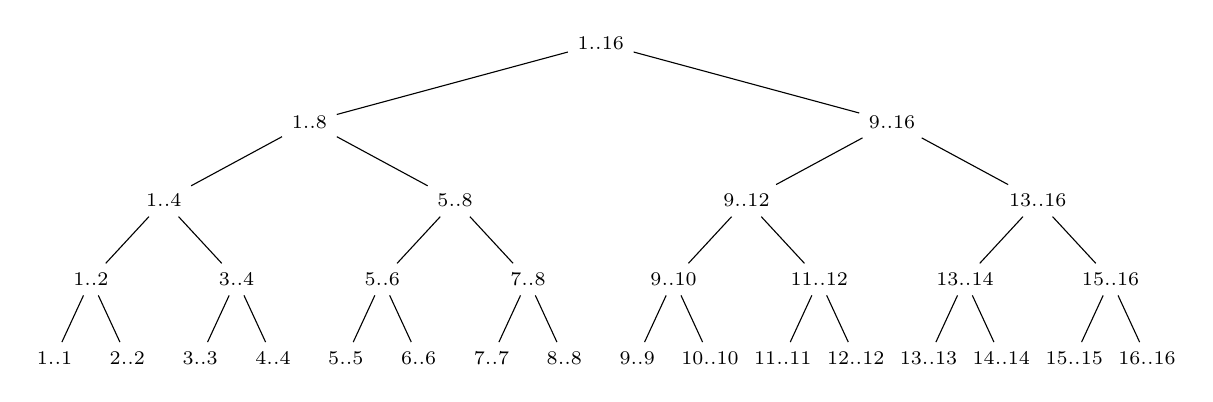
\begin{tikzpicture}[
	level/.append style = {level distance=10mm, sibling distance=148mm/2^#1},
	every node/.append style = {font=\scriptsize}
]

\node (root) {$1..16$}
	child {node {$1..8$}
		child {node {$1..4$}
			child {node {$1..2$}
				child {node {$1..1$}}
				child {node {$2..2$}}
			}
			child {node {$3..4$}
				child {node {$3..3$}}
				child {node {$4..4$}}
			}
		}
		child {node {$5..8$}
			child {node {$5..6$}
				child {node {$5..5$}}
				child {node {$6..6$}}
			}
			child {node {$7..8$}
				child {node {$7..7$}}
				child {node {$8..8$}}
			}
		}
	}
	child {node {$9..16$}
		child {node {$9..12$}
			child {node {$9..10$}
				child {node {$9..9$}}
				child {node {$10..10$}}
			}
			child {node {$11..12$}
				child {node {$11..11$}}
				child {node {$12..12$}}
			}
		}
		child {node {$13..16$}
			child {node {$13..14$}
				child {node {$13..13$}}
				child {node {$14..14$}}
			}
			child {node {$15..16$}
				child {node {$15..15$}}
				child {node {$16..16$}}
			}
		}
	};

\end{tikzpicture}

	\caption{Drzewo rekursji dla procedury \proc{Merge-Sort} działającej na tablicy z~16 elementami.
Każdy węzeł drzewa jest oznaczony przez zakres $i\twodots j$ tablicy, na której działa procedura.} \label{fig:15.3-2}
\end{figure}

\exercise %15.3-3
Problem ten ma własność optymalnej podstruktury, o~czym można się przekonać podobnie, jak w~jego oryginalnej wersji.
W~tym wariancie optymalnym nawiasowaniem iloczynu macierzy będziemy nazywać takie nawiasowanie, które maksymalizuje liczbę mnożeń skalarnych.

Przypuśćmy, że w~optymalnym nawiasowaniu iloczynu $A_iA_{i+1}\dots A_j$ podział występuje między $A_k$ i~$A_{k+1}$.
Wówczas nawiasowanie początkowego podciągu $A_iA_{i+1}\dots A_k$, stanowiące część optymalnego nawiasowania iloczynu $A_iA_{i+1}\dots A_j$, musi być optymalne.
Gdyby bowiem istniał sposób ustawienia nawiasów w~ciągu $A_iA_{i+1}\dots A_k$ o~większym koszcie, to podmieniając nawiasowanie tego podciągu w~optymalnym nawiasowaniu $A_iA_{i+1}\dots A_j$, otrzymalibyśmy inne nawiasowanie dla $A_iA_{i+1}\dots A_j$, ale o~koszcie większym niż optymalny, co stanowi sprzeczność z~założeniem.
Podobne rozumowanie prowadzi do wniosku, że nawiasowanie podciągu $A_{k+1}A_{k+2}\dots A_j$ w~optymalnym nawiasowaniu $A_iA_{i+1}\dots A_j$ jest optymalne dla ciągu $A_{k+1}A_{k+2}\dots A_j$.

\exercise %15.3-4
W~problemie planowania czynności na liniach montażowych zarówno najszybszy sposób montażu do stanowiska $S_{1,j}$, jak i~najszybszy sposób montażu do stanowiska $S_{2,j}$, polega na optymalnych czasach montażu do stanowisk $S_{1,j-1}$ i~$S_{2,j-1}$.
Innymi słowy, wartości $f_1[j-1]$ oraz $f_2[j-1]$ wykorzystywane są do obliczenia zarówno $f_1[j]$, jak i~$f_2[j]$.

\exercise %15.3-5
Jednym z~kontrprzykładów jest ciąg macierzy $\langle A_1,A_2,A_3\rangle$ o~rozmiarach stanowiących ciąg $\langle1,2,5,4\rangle$.
Liczbą mnożeń skalarnych wykonywanych podczas mnożenia $A_1$ przez $(A_2A_3)$ jest $1\cdot2\cdot4=8$, a~podczas mnożenia $(A_1A_2)$ przez $A_3$ -- $1\cdot5\cdot4=20$.
W~podejściu zachłannym podział iloczynu $A_1A_2A_3$ zostanie zatem wyznaczony między macierzą $A_1$ a~$A_2$ i~wynikowym nawiasowaniem będzie $(A_1(A_2A_3))$ z~kosztem $2\cdot5\cdot4+1\cdot2\cdot4=48$ mnożeń skalarnych.
Rozwiązaniem optymalnym jest jednak nawiasowanie $((A_1A_2)A_3)$ o~koszcie $1\cdot2\cdot5+1\cdot5\cdot4=30$.

\subchapter{Najdłuższy wspólny podciąg}

\exercise %15.4-1
Dla zadanych ciągów NWP wyznaczonym przez procedury \proc{LCS-Length} i~\proc{Print-LCS} jest $\langle1,0,0,1,1,0\rangle$.
Poza nim istnieje jeszcze 7 innych NWP tych ciągów:
\begin{gather*}
	\langle0,0,1,0,1,0\rangle, \langle0,0,1,0,1,1\rangle, \langle0,0,1,1,0,1\rangle, \langle0,1,0,1,0,1\rangle, \\
	\langle1,0,1,0,1,0\rangle, \langle1,0,1,0,1,1\rangle, \langle1,0,1,1,0,1\rangle.
\end{gather*}

\exercise %15.4-2
Poniższy pseudokod stanowi implementację zmodyfikowanej wersji procedury \proc{Print-LCS}, która wypisuje NWP ciągów $X$, $Y$ bez korzystania z~tablicy $b$.
\begin{codebox}
\Procname{$\proc{Print-LCS}'(c,X,Y,i,j)$}
\li	\If $i=0$ lub $j=0$
\li		\Then \Return
		\End
\li	\If $x_i=y_j$
\li		\Then $\proc{Print-LCS}'(c,X,Y,i-1,j-1)$
\li			wypisz $x_i$
\li		\ElseIf $c[i,j]=c[i-1,j]$
\li			\Then $\proc{Print-LCS}'(c,X,Y,i-1,j)$
\li		\ElseNoIf $\proc{Print-LCS}'(c,X,Y,i,j-1)$
		\End
\end{codebox}

\exercise %15.4-3
W~naszej implementacji będziemy obliczać kolejne wartości rekurencyjnie bezpośrednio ze wzoru (15.14), ale z~wykorzystaniem tablicy $c[1\twodots m,1\twodots n]$ i~mechanizmu spamiętywania.
Aby zaznaczyć, że dane pole tablicy $c$ nie zostało jeszcze obliczone, użyjemy specjalnej wartości $\infty$.
Pierwsza z~procedur inicjalizuje tablicę $c$, po czym wywołuje właściwy algorytm odpowiedzialny za obliczenie wartości $c[m,n]$.
\begin{codebox}
\Procname{$\proc{Memoized-LCS-Length}(X,Y)$}
\li	$m\gets\attrib{X}{length}$
\li	$n\gets\attrib{Y}{length}$
\li	\For $i\gets0$ \To $m$
\li		\Do \For $j\gets0$ \To $n$
\li				\Do $c[i,j]\gets\infty$ \label{li:memoized-lcs-length-init}
				\End
		\End
\li	\Return $\proc{Lookup-LCS}(c,X,Y,m,n)$
\end{codebox}
\begin{codebox}
\Procname{$\proc{Lookup-LCS}(c,X,Y,i,j)$}
\li	\If $c[i,j]<\infty$
\li		\Then \Return $c[i,j]$
		\End
\li	\If $i=0$ lub $j=0$
\li		\Then $c[i,j]\gets0$
\li		\ElseIf $x_i=y_j$
\li			\Then $c[i,j]\gets\proc{Lookup-LCS}(c,X,Y,i-1,j-1)+1$
\li		\ElseNoIf $c[i,j]\gets\max(\proc{Lookup-LCS}(c,X,Y,i,j-1),\proc{Lookup-LCS}(c,X,Y,i-1,j))$
		\End
\li	\Return $c[i,j]$
\end{codebox}

Każde z~$(m+1)(n+1)$ pól tablicy $c$ zostaje zainicjalizowane w~wierszu \ref{li:memoized-lcs-length-init}, a~następnie zmodyfikowane przez jedno wywołanie procedury \proc{Lookup-LCS}.
Wywołania procedury \proc{Lookup-LCS} możemy podzielić na dwa typy:
\begin{enumerate}
	\item wywołania, w~których $c[i,j]=\infty$, oraz
	\item wywołania, w~których $c[i,j]<\infty$.
\end{enumerate}
Wywołań pierwszego typu jest dokładnie $\Theta(mn)$, jedno na każde pole tablicy $c$.
Wszystkie wywołania drugiego typu pojawiają się jako rekurencyjne wywołania w~wywołaniach pierwszego typu.
Kiedy w~danym wywołaniu \proc{Lookup-LCS} pojawiają się wywołania rekurencyjne, jest ich $\Theta(1)$, dlatego łącznie wywołań drugiego typu jest $\Theta(mn)$.
Każde wywołanie drugiego typu zabiera czas $\Theta(1)$, a~każde wywołanie pierwszego typu jest wykonywane w~czasie $O(1)$ plus czas spędzany na obliczenia rekurencyjne.
Dlatego łączny czas wykonania algorytmu \proc{Memoized-LCS-Length} wynosi $\Theta(mn)$.

\exercise %15.4-4
\exercise %15.4-5
\exercise %15.4-6

\subchapter{Optymalne drzewa wyszukiwań binarnych}

\exercise %15.5-1
\exercise %15.5-2
\exercise %15.5-3
\exercise %15.5-4


\problems

\problem{Bitoniczny problem komiwojażera} %15-1
W~naszym rozwiązaniu przyjmujemy, że żadne dwa punkty wejściowe nie mają tej samej współrzędnej $x$.
Podążając za wskazówką z~treści problemu, będziemy przeglądać punkty wejściowe od lewej do prawej, po uprzednim posortowaniu ich po współrzędnych $x$.
Ciąg tak uporządkowanych punktów oznaczymy przez $\langle p_1,p_2,\dots,p_n\rangle$, czyli $p_1$ jest punktem wysuniętym najbardziej na lewo, a~$p_n$ punktem wysuniętym najbardziej na prawo.

Oznaczmy przez $B_{i,j}$, gdzie $i\le j$, zbiór ścieżek bitonicznych zawierających wszystkie punkty $p_1$, $p_2$, \dots, $p_j$, które zaczynają się w~pewnym punkcie $p_i$, biegną następnie ciągle w~lewo (czyli po punktach o~coraz mniejszych współrzędnych $x$) do punktu $p_1$, a~następnie ciągle w~prawo (czyli po punktach o~coraz większych współrzędnych $x$) do punktu $p_j$.
Przez $|p_ip_j|$ oznaczymy odległość euklidesową między punktami $p_i$ i~$p_j$, a~przez $b[i,j]$, gdzie $1\le i\le j\le n$, długość najkrótszej ścieżki bitonicznej ze zbioru $B_{i,j}$.
Zauważmy, że zbiór $B_{1,j}$ zawiera tylko jedną ścieżkę, dlatego $b[1,j]=\sum_{k=2}^j|p_{k-1}p_k|$.
Jedyną wartością $b[i,i]$, której będziemy potrzebować, jest $b[n,n]$, co stanowi długość szukanego najkrótszego cyklu bitonicznego dla wejściowego zbioru punktów.

Rozważmy najkrótszą ścieżkę bitoniczną $\beta$ z~$B_{i,j}$ i~zastanówmy się nad położeniem na niej punktu $p_{j-1}$.
Jeśli znajduje się on na podścieżce biegnącej w~prawo, to poprzedza on bezpośrednio punkt $p_j$ na tej podścieżce.
Podścieżka od $p_i$ do $p_{j-1}$ musi być najkrótszą ścieżką bitoniczną z~$B_{i,j-1}$, inaczej moglibyśmy ją ,,wyciąć'' i~,,wkleić'' w~jej miejsce podścieżkę bitoniczną o~mniejszej długości, uzyskując ścieżkę krótszą niż $\beta$.
Stąd długość $b[i,j]$ ścieżki $\beta$ wynosi $b[i,j-1]+|p_{j-1}p_j|$.
W~przeciwnym przypadku $p_{j-1}$ musi być najbardziej w~prawo wysuniętym punktem podścieżki biegnącej w~lewo, czyli $i=j-1$.
Bezpośrednio przed $p_j$ na podścieżce biegnącej w~prawo mamy więc $p_k$, gdzie $k<j-1$.
Tutaj także ma miejsce optymalna podstruktura -- podścieżka z~$p_k$ do $p_{j-1}$ jest najkrótszą ścieżką bitoniczną z~$B_{k,j-1}$, o~czym można się przekonać stosując metodę ,,wytnij i~wklej''.
W~tym przypadku ścieżka $\beta$ ma długość $b[i,j]=\min_{1\le k<j-1}(b[k,j-1]+|p_kp_j|)$.
Zachodzi zatem następująca zależność rekurencyjna:
\[
	b[i,j] = \begin{cases}
		|p_1p_2|, & \text{jeśli $i=1$, $j=2$}, \\
		\displaystyle\min_{1\le k<j-1}(b[k,j-1]+|p_kp_j|), & \text{jeśli $i=j-1>1$}, \\
		b[i,j-1]+|p_{j-1}p_j|, & \text{jeśli $i<j-1$}.
	\end{cases}
\]
W~szukanym optymalnym cyklu bitonicznym, jednym z~punktów sąsiadujących z~$p_n$ jest $p_{n-1}$, skąd $b[n,n]=b[n,n-1]+|p_{n-1}p_n|$.

Aby zrekonstruować rozwiązanie, będziemy obliczać wartości $r[i,j]$ -- indeks punktu bezpośrednio poprzedzającego $p_j$ na najkrótszej ścieżce z~$B_{i,j}$.
Poniższy pseudokod wyznacza wartości $b[i,j]$ i~$r[i,j]$, wykorzystując programowanie dynamiczne.
\begin{codebox}
\Procname{$\proc{Bitonic-TSP}(p,n)$}
\li	posortuj ciąg punktów wejściowych $p$ rosnąco względem ich współrzędnych $x$
\li	$b[1,2]\gets|p_1p_2|$
\li	\For $j\gets3$ \To $n$
\li		\Do \For $i\gets1$ \To $j-2$
\li			\Do $b[i,j]\gets b[i,j-1]+|p_{j-1}p_j|$
\li				$r[i,j]\gets j-1$
			\End
\li			$b[j-1,j]\gets\infty$
\li			\For $k\gets1$ \To $j-2$
\li				\Do $q\gets b[k,j-1]+|p_kp_j|$
\li					\If $q<b[j-1,j]$
\li						\Then $b[j-1,j]\gets q$
\li							$r[j-1,j]\gets k$
						\End
				\End
		\End
\li	$b[n,n]\gets b[n,n-1]+|p_{n-1}p_n|$
\li	\Return $b$ i~$r$
\end{codebox}

Znalezione rozwiązanie wypiszemy, zaczynając od $p_n$, następnie wypiszemy punkty na podścieżce biegnącej w~lewo, która zawiera $p_{n-1}$, aż do $p_1$, a~następnie pozostałe punkty z~podścieżki biegnącej w~prawo aż do $p_n$.
\begin{codebox}
\Procname{$\proc{Print-Bitonic-Tour}(r,n)$}
\li	wypisz $p_n$
\li	wypisz $p_{n-1}$
\li	$\proc{Print-Bitonic-Path}(r,r[n-1,n],n-1)$
\li	wypisz $p_{r[n-1,n]}$
\end{codebox}
\begin{codebox}
\Procname{$\proc{Print-Bitonic-Path}(r,i,j)$}
\li	\If $i<j$
\li		\Then wypisz $p_{r[i,j]}$
\li			\If $r[i,j]>1$
\li				\Then $\proc{Print-Bitonic-Path}(r,i,r[i,j])$
				\End
\li		\Else \If $r[j,i]>1$
\li				\Then $\proc{Print-Bitonic-Path}(r,r[j,i],j)$
\li					wypisz $p_{r[j,i]}$
				\End
		\End
\end{codebox}
W~wywołaniu $\proc{Print-Bitonic-Path}(r,i,j)$, jeśli $i<j$, to procedura ta wypisuje podścieżkę biegnącą w~lewo, a~jeśli $i>j$, to podścieżkę biegnącą w~prawo.

Czas działania algorytmu \proc{Bitonic-TSP} wynosi $O(n^2)$, gdyż zewnętrzna pętla wykonuje $n-2$ iteracje, a~każda wewnętrzna pętla wykonuje co najwyżej $n-2$ iteracji.
Sortowanie punktów na samym początku algorytmu można wykonać w~czasie $O(n\lg n)$, co nie wpływa na powyższe oszacowanie.
Wypisanie znalezionego cyklu za pomocą procedury \proc{Print-Tour} odbywa się w~czasie $O(n)$, dlatego że każdy punkt wypisywany jest dokładnie raz.

\problem{Estetyczny wydruk} %15-2
Danymi wejściowymi w~naszym rozwiązaniu będzie ciąg $l$ długości słów wejściowych oraz pojemność wiersza $M$.
Przedstawiony algorytm można nietrudno przekształcić tak, aby przyjmował rzeczywisty akapit tekstu i~wypisywał jego słowa podzielone na linie.
Zakładamy ponadto, że każde słowo z~tego akapitu mieści się w~wierszu, tzn.\ $l_i\le M$ dla każdego $i=1$, 2, \dots, $n$.

Zdefiniujmy $\id{extras}[i,j]$, gdzie $i\le j$, jako liczbę zbędnych znaków odstępu na końcu wiersza zawierającego słowa o~numerach od $i$ do $j$, czyli $\id{extras}[i,j]=M-j+i-\sum_{k=i}^jl_k$.
Z~kolei $\id{lc}[i,j]$ niech będzie kosztem wprowadzanym przez wiersz ze słowami od $i$ do $j$.
Przyjmiemy, że $\id{lc}[i,j]=\infty$, jeśli słowa te nie mieszczą się w~wierszu -- taki zabieg sprawi, że podczas minimalizacji tych wartości przepełnione wiersze nie będą wybierane.
Ostatni wiersz, jeśli nie jest przepełniony, wprowadza zerowy koszt, zgodnie ze specyfikacją problemu.
Mamy więc:
\[
	\id{lc}[i,j] = \begin{cases}
		\infty, & \text{jeśli $\id{extras}[i,j]<0$}, \\
		0, & \text{jeśli $j=n$ i~$\id{extras}[i,j]\ge0$}, \\
		(\id{extras[i,j]})^3, & \text{w~pozostałych przypadkach}.
	\end{cases}
\]

Naszym zadaniem jest minimalizacja sumy wartości \id{lc} po wszystkich wierszach, na jakie można podzielić tekst wejściowy.
Rozważmy optymalne rozmieszczenie słów o~numerach od 1 do $j$, gdzie $1\le j\le n$.
Niech $i$ będzie numerem słowa, które rozpoczyna ostatni wiersz w~takim podziale.
Poprzednie wiersze, o~ile istnieją, składają się zatem ze słów od 1 do $i-1$ i~rozmieszczenie ich w~wierszach musi być optymalne, co można uzasadnić za pomocą metody ,,wytnij i~wklej''.
Niech $c[j]$ będzie kosztem optymalnego układu słów od 1 do $j$.
Jeśli ostatni wiersz rozpoczyna słowo o~numerze $i$, to $c[j]=c[i-1]+\id{lc}[i,j]$.
Odpowiednią wartość $i$ minimalizującą $c[j]$ można wyznaczyć, sprawdzając każdy numer od 1 do $j$ i~wybierając optymalny z~nich.
Możemy ponadto przyjąć $c[0]=0$ jako brzegowy przypadek tej rekurencji:
\[
	c[j] = \begin{cases}
		0, & \text{jeśli $j=0$}, \\
		\displaystyle\min_{1\le i\le j}(c[i-1]+\id{lc}[i,j]), & \text{jeśli $j>0$}.
	\end{cases}
\]
Jej wartości możemy przechowywać w~tablicy i~obliczać od lewej do prawej.

Zaobserwujmy jednak, że wiersz może zawierać co najwyżej $\lceil M/2\rceil$ słów.
W~wierszu składającym się z~$j-i+1$ słów o~numerach od $i$ do $j$, jeśli $j-i+1>\lceil M/2\rceil$, to wiadomo, że $\id{lc}[i,j]=\infty$.
Stąd podczas obliczania $c[j]$ można tak naprawdę ograniczyć zakres sprawdzanych numerów $i$ od dołu przez $\max(1,j-\lceil M/2\rceil+1)$.

Zauważmy też, że możemy zrezygnować z~tablic \id{extras} oraz \id{lc} i~pamiętać jedynie potrzebne w~danej chwili wartości.
Posłużymy się w~tym celu ciągiem sum prefiksowych długości słów, który przechowamy w~tablicy $L[0\twodots n]$.
Dokładniej, dla każdego $j=0$, 1, \dots, $n$, $L[j]=\sum_{k=1}^jl_k$.
Zdefiniowane wcześniej $\id{extras}[i,j]$ wynosi wówczas $M-j+i-(L[j]-L[i-1])$ i~wartość tę można wyznaczyć w~czasie stałym.
Podobnie wartości z~tablicy \id{lc} można wyliczać na bieżąco, ponieważ w~danym momencie wykorzystywana jest tylko jedna z~nich.

Do zapamiętywania, na~których pozycjach wejściowego ciągu następuje podział na wiersze, wykorzystamy dodatkową tablicę $p$.
W~trakcie obliczania $c[j]$, jeśli $c[j]=c[i-1]+\id{lc}[i,j]$, to do $p[j]$ wpiszemy $i$.
Dzięki temu będziemy wiedzieć, że ostatni wiersz w~znalezionym rozwiązaniu zawiera słowa o~numerach od $p[n]$ do $n$, przedostatni -- słowa o~numerach od $p[p[n]-1]$ do $p[n]-1$ itd.

\begin{codebox}
\Procname{$\proc{Break-Lines}(l,M)$}
\li	$n\gets\attrib{l}{length}$
\li	$L[0]\gets0$
\li	\For $i\gets1$ \To $n$
\li		\Do $L[i]\gets L[i-1]+l_i$
		\End
\li	$c[0]\gets0$
\li	\For $j\gets1$ \To $n$
\li		\Do $c[j]\gets\infty$
\li			$j_0\gets\max(1,j-\lceil M/2\rceil+1)$
\li			\For $i\gets j_0$ \To $j$
\li				\Do $\id{extras}\gets M-j+i-(L[j]-L[i-1])$
\li					\If $\id{extras}<0$
\li						\Then $\id{lc}\gets\infty$
\li					\ElseIf $j=n$
\li						\Then $\id{lc}\gets0$
\li					\ElseNoIf $\id{lc}\gets\id{extras}^3$
						\End
\li					\If $c[i-1]+\id{lc}<c[j]$
\li						\Then $c[j]\gets c[i-1]+\id{lc}$
\li							$p[j]\gets i$
						\End
				\End
		\End
\li	\Return $c$ i~$p$
\end{codebox}

Analizując liczbę wykonywanych iteracji poszczególnych pętli, można przekonać się o~tym, że czasowa złożoność algorytmu wynosi $O(nM)$, a~pamięciowa -- $\Theta(n)$.
Wypisanie znalezionego rozwiązania w~postaci ciągu numerów słów rozpoczynających kolejne wiersze realizuje wywołanie $\proc{Print-Lines}(p,n)$ poniższej procedury rekurencyjnej.
\begin{codebox}
\Procname{$\proc{Print-Lines}(p,j)$}
\li	\If $p[j]>1$
\li		\Then $\proc{Print-Lines}(p,p[j]-1)$
		\End
\li	wypisz $p[j]$
\end{codebox}
Ponieważ drugi argument jest zmniejszany w~kolejnych wywołaniach rekurencyjnych, to czasem działania tej procedury jest $O(n)$.

\problem{Odległość redakcyjna} %15-3

\subproblem %15-3(a)
Podobnie jak w~problemie NWP, będziemy korzystać z~notacji $X_i$ jako \singledash{$i$}{tego} prefiksu słowa $x$ oraz $Y_j$ jako \singledash{$j$}{tego} prefiksu słowa $y$.
W~podproblemach, jakie się pojawią, będziemy wyznaczać odległość redakcyjną prefiksów $X_i$ i~$Y_j$.

Niech $c[i,j]$ będzie optymalnym kosztem przekształcenia $X_i$ do $Y_j$.
Załóżmy, że $i$, $j>0$ i~że znana jest ostatnia operacja w~tym przekształceniu.
Jeśli operacją tą było kopiowanie lub zastąpienie znaku innym, to problemem do rozwiązania pozostaje znalezienie odległości redakcyjnej $X_{i-1}$ i~$Y_{j-1}$.
Można to stwierdzenie uzasadnić rozumowaniem ,,wytnij i~wklej''.
Zatem $c[i,j]=c[i-1,j-1]+\mathrm{koszt}(\text{skopiuj})$ w~przypadku, gdy znak $x[i]$ został skopiowany  do $y[j]$ oraz $c[i,j]=c[i-1,j-1]+\mathrm{koszt}(\text{zastąp})$, jeśli $x[i]$ został zastąpiony przez inny znak $y[j]$.
W~przypadku usuwania znaku podproblem stanowi wyznaczenie odległości redakcyjnej między $X_{i-1}$ a~$Y_j$, skąd $c[i,j]=c[i-1,j]+\mathrm{koszt}(\text{usuń})$.
Podobnie, jeśli ostatnio wstawiany był nowy znak, to podproblemem jest odległość $X_i$ od $Y_{j-1}$ i~wówczas $c[i,j]=c[i,j-1]+\mathrm{koszt}(\text{wstaw})$.
Do zamiany znaków doszło, gdy $x[i]=y[j-1]$ oraz $x[i-1]=y[j]$, o~ile $i$, $j\ge2$.
Wystarczy w~tym przypadku obliczyć odległość między słowami $X_{i-2}$ i~$Y_{j-2}$, a~następnie dodać do niej koszt operacji zamiany: $c[i,j]=c[i-2,j-2]+\mathrm{koszt}(\text{zamień})$.
W~końcu, jeśli ostatnią operacją było wyrzucenie reszty słowa $X_i$, to znaczy to, że konwersja z~$X_m$ do $Y_n$ została zakończona, czyli w~momencie wykonania tej operacji było $i=m$ oraz $j=n$.
Jeśli potraktujemy wyrzucenie reszty słowa jako wielokrotne usuwanie ostatniego jego znaku, to przekonamy się, że podproblem stanowi w~tym przypadku każde przekształcenie z~$X_k$ do $Y_n$, gdzie $0\le k<m$.
Mamy zatem $c[m,n]=\min_{0\le k<m}(c[k,n])+\mathrm{koszt}(\text{wyrzuć})$.
Na podstawie tej analizy otrzymujemy następującą zależność rekurencyjną:
\[
	c[i,j] = \min\begin{cases}
		c[i-1,j-1]+\mathrm{koszt}(\text{skopiuj}), & \text{jeśli $x[i]=y[j]$}, \\
		c[i-1,j-1]+\mathrm{koszt}(\text{zastąp}), & \text{jeśli $x[i]\ne y[j]$}, \\
		c[i-1,j]+\mathrm{koszt}(\text{usuń}), \\
		c[i,j-1]+\mathrm{koszt}(\text{wstaw}), \\
		c[i-2,j-2]+\mathrm{koszt}(\text{zamień}), & \text{jeśli $i$, $j\ge2$, $x[i]=y[j-1]$ i~$x[i-1]=y[j]$}, \\
		\displaystyle\min_{0\le k<m}(c[k,n])+\mathrm{koszt}(\text{wyrzuć}), & \text{jeśli $i=m$ i~$j=n$}.
	\end{cases}
\]

Rozważmy teraz sytuacje z~$i=0$ lub $j=0$.
Jeśli $i=0$, to prefiks $X_i$ jest słowem pustym i~przekształcenie go do słowa $Y_j$ polega na wykonaniu $j$ operacji wstawienia znaku, czyli $c[0,j]=j\cdot\mathrm{koszt}(\text{wstaw})$.
Podobnie, jeśli $j=0$, to słowo $Y_j$ jest puste i~można je uzyskać poprzez \singledash{$i$}{krotne} usunięcie znaku ze słowa $X_i$, czyli $c[i,0]=i\cdot\mathrm{koszt}(\text{usuń})$.

Poniższy pseudokod wypełnia tablicę $c$ od najwyższego do najniższego wiersza oraz od lewej do prawej w~obrębie wierszy.
Równocześnie konstruowana jest także tablica $\id{op}[0\twodots m,0\twodots n]$, w~której po zakończeniu działania algorytmu na pozycji $\id{op}[i,j]$ znajdzie się ostatnia operacja użyta do przekształcenia $X_i$ do $Y_j$, a~także tablice $l[0\twodots m,0\twodots n]$ i~$r[0\twodots m,0\twodots n]$ przechowujące rozmiary rozważanych podproblemów podczas tych przekształceń.

\begin{codebox}
\Procname{$\proc{Edit-Distance}(x,y)$}
\li	$m\gets\attrib{x}{length}$
\li	$n\gets\attrib{y}{length}$
\li	\For $i\gets0$ \To $m$
\li		\Do $c[i,0]\gets i\cdot\mathrm{koszt}(\text{usuń})$
\li			$\langle\id{op}[i,0],l[i,0],r[i,0]\rangle\gets\langle$,,usuń''$,i-1,0\rangle$
		\End
\li	\For $j\gets1$ \To $n$
\li		\Do $c[0,j]\gets j\cdot\mathrm{koszt}(\text{wstaw})$
\li			$\langle\id{op}[0,j],l[0,j],r[0,j]\rangle\gets\langle$,,wstaw ''$y[j],0,j-1\rangle$
		\End
\li	\For $i\gets1$ \To $m$
\li		\Do \For $j\gets1$ \To $n$
\li				\Do $c[i,j]\gets\infty$
\li					\If $x[i]=y[j]$
\li						\Then $c[i,j]\gets c[i-1,j-1]+\mathrm{koszt}(\text{skopiuj})$
\li							$\langle\id{op}[i,j],l[i,j],r[i,j]\rangle\gets\langle$,,skopiuj''$,i-1,j-1\rangle$
						\End
\li					\If $x[i]\ne y[j]$ i~$c[i-1,j-1]+\mathrm{koszt}(\text{zastąp})<c[i,j]$
\li						\Then $c[i,j]\gets c[i-1,j-1]+\mathrm{koszt}(\text{zastąp})$
\li							$\langle\id{op}[i,j],l[i,j],r[i,j]\rangle\gets\langle$,,zastąp przez ''$y[j],i-1,j-1\rangle$
						\End
\li					\If $c[i-1,j]+\mathrm{koszt}(\text{usuń})<c[i,j]$
\li						\Then $c[i,j]\gets c[i-1,j]+\mathrm{koszt}(\text{usuń})$
\li							$\langle\id{op}[i,j],l[i,j],r[i,j]\rangle\gets\langle$,,usuń''$,i-1,j\rangle$
						\End
\li					\If $c[i,j-1]+\mathrm{koszt}(\text{wstaw})<c[i,j]$
\li						\Then $c[i,j]\gets c[i,j-1]+\mathrm{koszt}(\text{wstaw})$
\li							$\langle\id{op}[i,j],l[i,j],r[i,j]\rangle\gets\langle$,,wstaw ''$y[j],i,j-1\rangle$
						\End
\li					\If $i\ge2$ i~$j\ge2$ i~$x[i]=y[j-1]$ i~$x[i-1]=y[j]$
\zi	\phantom{\kw{if} $i\ge2$} i~$c[i-2,j-2]+\mathrm{koszt}(\text{zamień})<c[i,j]$
\li						\Then $c[i,j]\gets c[i-2,j-2]+\mathrm{koszt}(\text{zamień})$
\li							$\langle\id{op}[i,j],l[i,j],r[i,j]\rangle\gets\langle$,,zamień''$,i-2,j-2\rangle$
						\End
				\End
		\End
\li	\For $k\gets0$ \To $m-1$
\li		\Do \If $c[k,n]+\mathrm{koszt}(\text{wyrzuć})<c[m,n]$
\li				\Then $c[m,n]\gets c[k,n]+\mathrm{koszt}(\text{wyrzuć})$
\li					$\langle\id{op}[m,n],l[m,n],r[m,n]\rangle\gets\langle$,,wyrzuć''$,k,n\rangle$
				\End
		\End
\li	\Return $c$, \id{op}, $l$ i~$r$
\end{codebox}

Zarówno złożoność czasowa, jak i~pamięciowa tego algorytmu wynoszą $\Theta(mn)$.
Wypisanie optymalnego ciągu operacji przekształcających słowo $x$ do słowa $y$ realizuje następująca procedura.
Jej początkowym wywołaniem jest $\proc{Print-Operations}(\id{op},l,r,m,n)$.
Aby zapewnić odpowiednią kolejność, przed wypisaniem bieżącej operacji procedura wywoływana jest rekurencyjnie dla podproblemu na podstawie wartości w~tablicach $l$ i~$r$ wyznaczonych w~\proc{Edit-Distance}.
\begin{codebox}
\Procname{$\proc{Print-Operations}(\id{op},l,r,i,j)$}
\li	\If $i>0$ lub $j>0$
\li		\Then $\proc{Print-Operations}(\id{op},l,r,l[i,j],r[i,j])$
\li			wypisz $\id{op}[i,j]$
		\End
\end{codebox}

\subproblem %15-3(b)
Możemy sprowadzić problem optymalnego uliniowienia do problemu odległości redakcyjnej w~następujący sposób.
Załóżmy, że $x'$ i~$y'$ są wynikowymi sekwencjami DNA powstałymi w~wyniku optymalnego uliniowienia, odpowiednio, sekwencji $x$ i~$y$.
Jeśli $x'[j]=y'[j]$, to w~problemie odległości redakcyjnej możemy tę sytuację rozumieć jako skopiowanie znaku $x'[j]$.
Jeśli $x'[j]\ne y'[j]$ i~żaden z~tych znaków nie jest spacją, to mamy tutaj sytuację po zastąpieniu znaku $x'[j]$ przez znak $y'[j]$.
W~końcu, spację na pozycję $x'[j]$ można uzyskać przez wykonanie operacji wstawienia znaku $y'[j]$, a~spację na pozycji $y'[j]$ -- przez wykonanie operacji usunięcia znaku $x'[j]$.

Teraz wystarczy jeszcze przypisać odpowiednie koszty dla poszczególnych operacji elementarnych.
W~problemie optymalnego uliniowienia odpowiednio zdefiniowana ocena jest maksymalizowana, zaś problem odległości redakcyjnej ma na celu minimalizację odpowiadającego tej ocenie kosztu.
Wystarczy więc jako koszt wziąć liczbę przeciwną do odpowiadającej mu oceny.
Poszczególne operacje wartościujemy następująco:
\begin{align*}
	\mathrm{koszt}(\text{skopiuj}) &= -1, \\
	\mathrm{koszt}(\text{zamień}) &= +1, \\
	\mathrm{koszt}(\text{usuń}) &= +2, \\
	\mathrm{koszt}(\text{wstaw}) &= +2.
\end{align*}
Operacje zamień i~wyrzuć nie są wykorzystywane, więc jako ich koszt można przyjąć wartość $\infty$.

\problem{Planowanie bankietu w~firmie} %15-4
Ogólnie rzecz biorąc, naszym zamierzeniem w~tym problemie jest zapraszanie pracowników o~wysokim ,,współczynniku towarzyskości'', zaś wykluczanie takich, dla których współczynnik ten jest niski.
Dla każdego pracownika będziemy rozważać, czy opłaca się zaprosić go na bankiet.
Jeśli to zrobimy, to musimy wykluczyć z~bankietu wszystkich jego bezpośrednich podwładnych i~bezpośredniego przełożonego (o~ile ten istnieje).

Załóżmy, że dane wejściowe do problemu stanowi drzewo $T$ w~reprezentacji ,,na lewo syn, na prawo brat'', w~którym każdy węzeł $x$, oprócz wskaźników na inne węzły ma atrybut \id{name} przechowujący nazwisko pracownika oraz \id{conv} zawierający jego ,,współczynnik towarzyskości''.
Potraktujemy każde poddrzewo drzewa wejściowego jako podproblem naszego problemu i~rozwiążemy każdy z~nich, poruszając się od poddrzew składających się z~tylko jednego węzła (liścia drzewa $T$), aż do całego drzewa $T$.
Każdy węzeł $x$ drzewa $T$ wzbogacimy o~dwa dodatkowe pola -- \id{invited} oraz \id{uninvited}.
W~pierwszym z~nich obliczana będzie największa możliwa suma ,,współczynników towarzyskości'' dla podproblemu stanowiącego poddrzewo o~korzeniu $x$, przy założeniu, że osoba reprezentowana przez węzeł $x$ jest zaproszona na bankiet.
Rola atrybutu \id{uninvited} jest identyczna, ale dla sytuacji, w~której osoba $x$ nie zostaje zaproszona na bankiet.

Łatwo zauważyć, że dla dowolnego węzła $x$ w~$T$, gdzie $C_x$ jest zbiorem jego dzieci, zachodzą następujące zależności:
\begin{align*}
	\attrib{x}{invited} &= \attrib{x}{conv}+\sum_{y\in C_x}\attrib{y}{uninvited}, \\
	\attrib{x}{uninvited} &= \sum_{y\in C_x}\max(\attrib{y}{invited},\attrib{y}{uninvited}).
\end{align*}
Wówczas rozwiązaniem problemu jest $\max(\attribb{T}{root}{invited},\attribb{T}{root}{uninvited})$.

Nasz algorytm będzie przyjmował na wejściu węzeł $x$ drzewa $T$ i~wyznaczał pola \attrib{x}{invited} oraz \attrib{x}{uninvited}.
Algorytm wywołany zostanie w~tym celu rekurencyjnie po wszystkich dzieciach węzła $x$.
Zwracaną wartością będzie maksymalna suma ,,współczynników towarzyskości'' dla poddrzewa o~korzeniu w~$x$.
Wywołanie $\proc{Company-Party}(\attrib{T}{root})$ zwróci zatem rozwiązanie pełnego problemu.
\begin{codebox}
\Procname{$\proc{Company-Party}(x)$}
\li	$\attrib{x}{invited}\gets\attrib{x}{conv}$
\li	$\attrib{x}{uninvited}\gets0$
\li	$y\gets\attrib{x}{left-child}$
\li	\While $y\ne\const{nil}$
\li		\Do $\proc{Company-Party}(y)$
\li			$\attrib{x}{invited}\gets\attrib{x}{invited}+\attrib{y}{uninvited}$
\li			$\attrib{x}{uninvited}\gets\attrib{x}{uninvited}+\max(\attrib{y}{invited},\attrib{y}{uninvited})$
\li			$y\gets\attrib{y}{right-sibling}$
			\End
\li	\Return $\max(\attrib{x}{invited},\attrib{x}{uninvited})$
\end{codebox}

W~celu wypisania zaproszonych gości dla tak wzbogaconego drzewa $T$ używamy wywołania $\proc{Print-Guests}(\attrib{T}{root})$ następującej procedury:
\begin{codebox}
\Procname{$\proc{Print-Guests}(x)$}
\li	\If $\attrib{x}{invited}>\attrib{x}{uninvited}$
\li		\Then wypisz \attrib{x}{name}
\li			$y\gets\attrib{x}{left-child}$
\li			\While $y\ne\const{nil}$
\li				\Do $\proc{Print-Invited-Subordinates}(y)$
\li					$y\gets\attrib{y}{right-sibling}$
					\End
\li		\Else $\proc{Print-Invited-Subordinates}(x)$
			\End
\end{codebox}
Używana tu procedura pomocnicza \proc{Print-Invited-Subordinates} wypisuje optymalny zbiór zaproszonych pracowników z~zadanego poddrzewa przy założeniu, że osoba znajdująca się w~jego korzeniu nie jest zaproszona na bankiet.
\begin{codebox}
\Procname{$\proc{Print-Invited-Subordinates}(x)$}
\li	$y\gets\attrib{x}{left-child}$
\li	\While $y\ne\const{nil}$
\li		\Do $\proc{Print-Guests}(y)$
\li			$y\gets\attrib{y}{right-sibling}$
			\End
\end{codebox}

Każdy węzeł drzewa $T$ w~wywołaniu $\proc{Company-Party}(\attrib{T}{root})$ jest wskazywany przez $x$ w~dokładnie jednym wywołaniu rekurencyjnym oraz przez $y$ w~co najwyżej jednym wywołaniu rekurencyjnym.
Wynika stąd, że dla hierarchii $n$ pracowników firmy, algorytm wyznacza optymalne rozwiązanie w~czasie $\Theta(n)$.

\problem{Algorytm Viterbiego} %15-5

\subproblem %15-5(a)
Ścieżka w~grafie $G$ z~wierzchołka $v_0$, mająca zadaną etykietę $\langle\sigma_1,\sigma_2,\dots,\sigma_k\rangle$ istnieje wtedy i~tylko wtedy, gdy istnieje ścieżka o~etykiecie $\langle\sigma_2,\dots,\sigma_k\rangle$ z~pewnego sąsiada $v_1$ wierzchołka $v_0$ oraz $\sigma(v_0,v_1)=\sigma_1$.
Innymi słowy, w~problemie tym dla zadanego ciągu etykiet wykorzystywane są podproblemy dla o~1 krótszego sufiksu tego ciągu.

Procedura \proc{Find-Path}, której pseudokod znajduje się poniżej, przyjmuje na wejściu graf $G$ reprezentowany przez tablicę list sąsiedztwa \id{Adj}, wierzchołek początkowy $v$ grafu $G$, tablicę $s$ przechowującą ciąg etykiet oraz początkowy indeks $i$ tej tablicy.
Wywołanie $\proc{Find-Path}(G,v,s,i)$ będzie znajdować ścieżkę w~grafie $G$, zaczynającą się w~wierzchołku $v$ oraz mającą etykietę złożoną z~kolejnych elementów z~$s[i\twodots\attrib{s}{length}]$.
Przeglądani będą wszyscy sąsiedzi $w$ wierzchołka $v$ i~w~razie odnalezienia takiej krawędzi $\langle v,w\rangle$, której etykietą jest $\sigma_i$, procedura wywołana zostanie rekurencyjnie dla wierzchołka $w$ oraz ze zwiększonym o~1 indeksem $i$.
W~przypadku odnalezienia ścieżki dla któregokolwiek sąsiada $v$, zostanie ona skonkatenowana z~$v$ i~zwrócona jako wynik procedury.
W~przeciwnym wypadku zwrócona zostanie specjalna wartość \const{nie-ma-takiej-ścieżki}.
\begin{codebox}
\Procname{$\proc{Find-Path}(G,v,s,i)$}
\li	\If $i=\attrib{s}{length}+1$
\li		\Then \Return $v$
		\End
\li	\For każdy $w\in\id{Adj}[v]$
\li		\Do \If $\sigma(v,w)=\sigma_i$
\li				\Then $\id{path}\gets\proc{Find-Path}(G,w,s,i+1)$
\li					\If $\id{path}\ne\const{nie-ma-takiej-ścieżki}$
\li						\Then \Return $v$, \id{path}
						\End
				\End
		\End
\li	\Return \const{nie-ma-takiej-ścieżki}
\end{codebox}
Aby rozwiązać problem dla grafu $G=\langle V,E\rangle$ z~wyróżnionym wierzchołkiem $v_0\in V$ oraz etykiety przechowywanej w~tablicy $s$, należy wywołać $\proc{Find-Path}(G,v_0,s,1)$.

Każdy podproblem, jaki może się pojawić, ma na celu znalezienie ścieżki o~zadanej długości $k$, zaczynającej się w~pewnym wierzchołku grafu $G=\langle V,E\rangle$.
Istnieje zatem $k|V|$ możliwych podproblemów, a~podczas rozwiązywania dowolnego z~nich może być sprawdzana krawędź do każdego innego wierzchołka grafu $G$.
Czas działania algorytmu wynosi stąd $O(k|V|^2)$.

\subproblem %15-5(b)
W~tej modyfikacji, zamiast kończyć wyszukiwanie ścieżki w~momencie odnalezienia jakiejkolwiek o~zadanej etykiecie, będziemy sprawdzać możliwe krawędzie wychodzące z~wierzchołka wejściowego.
Optymalna podstruktura wygląda podobnie do tej z~oryginalnej wersji problemu z~punktu (a).
Następujący algorytm opiera się na \proc{Find-Path} i~realizuje opisane podejście.
Zwraca on ścieżkę o maksymalnym możliwym prawdopodobieństwie, a~także samą wartość tego prawdopodobieństwa.
\begin{codebox}
\Procname{$\proc{Viterbi}(G,v,s,i)$}
\li	\If $i=\attrib{s}{length}+1$
\li		\Then \Return $v$, 1
		\End
\li	$\id{path}\gets\const{nie-ma-takiej-ścieżki}$
\li	$\id{prob}\gets0$
\li	\For każdy $w\in\id{Adj}[v]$
\li		\Do \If $\sigma(v,w)=\sigma_i$
\li				\Then $\id{path}'$, $\id{prob}'\gets\proc{Viterbi}(G,w,s,i+1)$
\li					\If $p(v,w)\cdot\id{prob}'\ge\id{prob}$
\li						\Then $\id{prob}\gets p(v,w)\cdot\id{prob}'$
\li							$\id{path}\gets v$, $\id{path}'$
						\End
				\End
		\End
\li	\Return \id{path}, \id{prob}
\end{codebox}

Czas działania tego algorytmu wynosi $O(k|V|^2)$, na podstawie identycznej analizy jak w~punkcie (a).

\problem{Przesuwanie pionka} %15-6
Ponumerujmy kolejnymi liczbami całkowitymi od 1 do $n$ wiersze z~dołu do góry, oraz kolumny z~lewej do prawej.
Każde pole szachownicy utożsamimy z~jego położeniem na szachownicy w~postaci pary $\langle i,j\rangle$, gdzie $i$ to numer wiersza tego pola, a~$j$ -- numer jego kolumny.
Zdefiniujmy $g[i,j]$ dla $1\le i$, $j\le n$ jako największą liczbę złotych możliwą do uzyskania, przechodząc pionkiem z~pewnego pola na dolnym brzegu szachownicy na pole $\langle i,j\rangle$, wykonując przy tym tylko dopuszczalne ruchy.
Oczywiście $g[1,j]=0$ dla $j=1$, 2, \dots, $n$.
Maksymalny zysk w~polu $\langle i,j\rangle$ możemy osiągnąć, przechodząc na nie z~pola $\langle i-1,j-1\rangle$ (o~ile $j>1$), $\langle i-1,j\rangle$ albo $\langle i-1,j+1\rangle$ (o~ile $j<n$).
Każda możliwość do sumarycznego zysku dodaje częściowy zysk związany z~przejściem na pole $\langle i,j\rangle$, zdefiniowanym przez funkcję $p$.
Dla $i=2$, 3, \dots, $n$ zachodzi następująca zależność:
\[
	g[i,j] = \max\begin{cases}
		g[i-1,j-1]+p(\langle i-1,j-1\rangle,\langle i,j\rangle), & \text{jeśli $j>1$,} \\
		g[i-1,j]+p(\langle i-1,j\rangle,\langle i,j\rangle), & \\
		g[i-1,j+1]+p(\langle i-1,j+1\rangle,\langle i,j\rangle), & \text{jeśli $j<n$.}
	\end{cases}
\]

W~naszym algorytmie zastosujemy programowanie dynamiczne w~celu obliczenia wartości w~tablicy $g$.
Ponadto w~tablicy $m$ będziemy przechowywać dane ułatwiające rekonstrukcję znalezionej ścieżki pionka.
Pozycja $m[i,j]$ będzie zawierać numer kolumny pola z~wiersza $i-1$, z~którego prowadzi optymalna ścieżka do pola $\langle i,j\rangle$.
Ponadto w~zmiennej $m^*\!$ po zakończeniu działania algorytmu znajdzie się numer kolumny pola na górnym brzegu szachownicy, na którym kończy się optymalna ścieżka pionka.
\begin{codebox}
\Procname{$\proc{Checkerboard}(n,p)$}
\li	\For $j\gets1$ \To $n$
\li		\Do $g[1,j]\gets0$
		\End
\li	\For $i\gets2$ \To $n$
\li		\Do \For $j\gets1$ \To $n$
\li				\Do $g[i,j]\gets g[i-1,j]+p(\langle i-1,j\rangle,\langle i,j\rangle)$
\li					$m[i,j]\gets j$
\li					\If $j>1$ i~$g[i-1,j-1]+p(\langle i-1,j-1\rangle,\langle i,j\rangle)>g[i,j]$
\li						\Then $g[i,j]\gets g[i-1,j-1]+p(\langle i-1,j-1\rangle,\langle i,j\rangle)$
\li							$m[i,j]\gets j-1$
						\End
\li					\If $j<n$ i~$g[i-1,j+1]+p(\langle i-1,j+1\rangle,\langle i,j\rangle)>g[i,j]$
\li						\Then $g[i,j]\gets g[i-1,j+1]+p(\langle i-1,j+1\rangle,\langle i,j\rangle)$
\li							$m[i,j]\gets j+1$
						\End
				\End
		\End
\li	$\id{result}\gets-\infty$
\li	$m^*\!\gets1$
\li	\For $j\gets1$ \To $n$
\li		\Do \If $g[n,j]>\id{result}$
\li				\Then $\id{result}\gets g[n,j]$
\li					$m^*\!\gets j$
				\End
		\End
\li	\Return $\id{result}$, $m$ i~$m^*\!$
\end{codebox}
Wykorzystując zwrócone wartości przez powyższy algorytm, możemy wypisać optymalną ścieżkę jako ciąg odwiedzonych pól, używając w~tym celu wywołania $\proc{Print-Moves}(m,n,m^*\!)$.
Pseudokod tej procedury przedstawiono poniżej.
\begin{codebox}
\Procname{$\proc{Print-Moves}(m,i,j)$}
\li	\If $i>1$
\li		\Then $\proc{Print-Moves}(m,i-1,m[i,j])$
		\End
\li	wypisz ,,$\langle$'' $i$ ,,{}, '' $j$ ,,$\rangle$''
\end{codebox}

Algorytm \proc{Checkerboard} wypełnia tablicę $g$, dla każdej z~$n^2$ jej komórek wykonując operacje w~czasie ograniczonym przez stałą.
Stąd czasem działania algorytmu jest $\Theta(n^2)$.

\problem{Planowanie prac} %15-7
Kluczowy w~naszym rozwiązaniu będzie następujący lemat:

\medskip
\noindent\textsf{\textbf{Lemat.}} \textit{W~uporządkowaniu o~maksymalnym zysku prace uszeregowane są według terminów ich ukończenia.}
\begin{proof}
Rozważmy optymalne uszeregowanie prac, w~którym praca $a_i$ jest wykonywana przed pracą $a_j$, ale $d_i>d_j$.
Zamiana $a_i$ z~$a_j$ w~tym uporządkowaniu może jedynie powiększyć zysk, dlatego możemy zamienić każdą taką parę, uzyskując w~wyniku zysk niemniejszy niż przez zamianą.
Ciąg, w~którym nie można już wykonać takiej zamiany, jest uporządkowaniem prac według terminów ich ukończenia.
\end{proof}

Posortujemy prace według ich terminów tak, aby zachodziło $d_1\le d_2\le\dots\le d_n$.
Zdefiniujemy $P[i,j]$ jako maksymalny zysk możliwy do osiągnięcia przez planowanie prac $\{a_1,a_2,\dots,a_i\}$ w~przedziale czasowym $[0,j]$.
Rozwiązaniem problemu jest wówczas $P[n,d_n]$, gdyż wykonanie dowolnej pracy po terminie jej ukończenia, a~w~szczególności po $d_n$, nie prowadzi do powiększenia sumarycznego zysku.
Z~tego samego powodu i~z~założenia, że czas wykonania każdej pracy wynosi co najwyżej $n$ jednostek czasu, możemy każdy termin wykonania $d_i$ zmniejszyć do $n^2$.

Zastanówmy się teraz, jak obliczyć wartość $P[i,j]$.
Jeśli $j<t_i$, to praca $a_i$ nie może być wykonana w~przedziale czasowym $[0,j]$, dlatego $P[i,j]=P[i-1,j]$.
Gdy jednak $j\ge t_i$, to możemy pominąć pracę $a_i$ w~naszym uporządkowaniu, co daje $P[i,j]=P[i-1,j]$.
Możemy też włączyć ją do uporządkowania, skąd na mocy powyższego lematu $P[i,j]$ jest równe sumie zysku wprowadzanego przez tę pracę oraz zysku z~podproblemu, w~którym przedział czasowy jest skrócony o~czas wykonania tej pracy, czyli $P[i,j]=p_i+P[i-1,j-t_i]$.

Dostajemy zależność rekurencyjną:
\[
	P[i,j] = \begin{cases}
		0, & \text{jeśli $i=1$, $j<t_i$}, \\
		p_1, & \text{jeśli $i=1$, $j\ge t_i$}, \\
		P[i-1,j], & \text{jeśli $i>1$, $j<t_i$}, \\
		\max(P[i-1,j],p_i+P[i-1,j-t_i]), & \text{jeśli $i>1$, $j\ge t_i$}.
	\end{cases}
\]
Można teraz łatwo ułożyć algorytm wykorzystujący programowanie dynamiczne, który wypełnia tablicę $P$ i~zwraca w~wyniku $P[n,d_n]$.
Tablica $P$ składa się z~$O(nd_n)=O(n^3)$ pozycji, dlatego czas wymagany do wypełnienia jej w~całości wynosi $O(n^3)$.

Założenie, z~którego korzystaliśmy w~zadaniu pozwoliło na zaprojektowanie wielomianowego algorytmu dla tego problemu.
W~ogólności, czyli przy dopuszczeniu dowolnie dużych czasów wykonania, problem staje się \singledash{NP}{zupełny} i~prawdopodobnie nie istnieje dla niego algorytm o~czasie niższym niż wykładniczy względem rozmiaru danych wejściowych.


% \chapter{Algorytmy zachłanne}

\makeatletter
\def\input@path{{chapter16/}}
\makeatother

\subchapter{Problem wyboru zajęć}
\note{W~procedurze \proc{Greedy-Activity-Selector} w~linii 1 zmienna\/ $n$ powinna przyjąć wartość\/ $\attrib{s}{length}-2$.
Wynika to z~tego, że tablica\/ $s$ składa się tak naprawdę z~\/$n+2$ elementów -- oprócz czasów rozpoczęcia \/$n$ rzeczywistych zajęć przechowuje także czasy fikcyjnych zajęć\/ $a_0$ i~\/$a_{n+1}$.}
\bignegskip

\exercise %16.1-1
W~poniższym algorytmie przyjmujemy, że zajęcia zostały uporządkowane niemalejąco według czasów zakończenia.
\begin{codebox}
\Procname{$\proc{Dynamic-Activity-Selector}(s,f)$}
\li	$n\gets\attrib{s}{length}-2$
\li	\For $l\gets2$ \To $n+2$ \label{li:dynamic-activity-selector-main-loop-begin}
\li		\Do \For $i\gets0$ \To $n-l+2$
\li				\Do $j\gets i+l-1$
\li					$c[i,j]\gets0$
\li					$A_{i,j}\gets\emptyset$
\li					\For $k\gets i+1$ \To $j-1$
\li						\Do $q\gets c[i,k]+c[k,j]+1$
\li							\If $f_i\le s_k<f_k\le s_j$ i~$q>c[i,j]$
\li								\Then $c[i,j]\gets q$
\li									$A_{i,j}\gets A_{i,k}\cup\{a_k\}\cup A_{k,j}$
								\End
						\End
				\End
		\End \label{li:dynamic-activity-selector-main-loop-end}
\li	\Return $A_{0,n+1}$
\end{codebox}
Algorytm oblicza wartości $c[i,j]$ oraz konstruuje zbiory $A_{i,j}$ dla $0\le i<j\le n+1$.
W~pierwszej iteracji pętli głównej (wiersze \doubledash{\ref{li:dynamic-activity-selector-main-loop-begin}}{\ref{li:dynamic-activity-selector-main-loop-end}}) dla $i=0$, 1, \dots, $n$ za pomocą równania (16.3) wyznaczane są wartości $c[i,i+1]$, a~na podstawie wzoru (16.2) zbiory $A_{i,i+1}$, czyli rozwiązywane są podproblemy składające się z~dokładnie dwóch zajęć.
W~kolejnej iteracji zostają wyznaczone rozwiązania podproblemów z~dokładnie trzema zajęciami itd.
Zwracanym wynikiem jest najliczniejszy zbiór zajęć stanowiący rozwiązanie podproblemu $S_{0,n+1}=S$.

Struktura pętli zaprezentowanego algorytmu przypomina tę z~procedury \proc{Matrix-Chain-Order} z~podrozdziału 15.2.
Można więc zastosować tu podobną analizę efektywności jak w~przypadku tamtej procedury i~dojść do oszacowania $\Theta(n^3)$ na czas działania naszego algorytmu -- znacznie wyższego od złożoności czasowej rozwiązania zachłannego.

\exercise %16.1-2
Załóżmy, że zajęcia $a_1$, $a_2$, \dots, $a_n$, wraz z~dwoma fikcyjnymi $a_0$ i~$a_{n+1}$, uporządkowane są według czasów rozpoczęcia, tzn.
\[
	s_0 \le s_1 \le s_2 \le \dots \le s_n \le s_{n+1}.
\]
Możemy wówczas udowodnić następujące twierdzenie analogiczne do tw.\ 16.1:

\bigskip
\noindent\textsf{\textbf{Twierdzenie 16.1$'$.}} \textit{Rozważmy niepusty podproblem\/ $S_{i,j}$ i~niech\/ $a_m$ będą zajęciami w~\/$S_{i,j}$ rozpoczynającymi się najpóźniej:
\[
	s_m = \max\bigl\{\,s_k:a_k\in S_{i,j}\,\bigr\}.
\]
Wtedy:
\begin{enumerate}
	\item Wśród najliczniejszych pozdbiorów parami zgodnych zajęć z~\/$S_{i,j}$ istnieje taki, który zawiera\/ $a_m$.
	\item Podproblem\/ $S_{m,j}$ jest pusty, tak więc po wybraniu\/ $a_m$ jedynym niepustym podproblemem może być tylko\/ $S_{i,m}$.
\end{enumerate}
}

Twierdzenie to mówi nam, że w~optymalnym rozwiązaniu podproblemu $S_{i,j}$, po wyborze zajęcia $a_m\in S_{i,j}$ rozpoczynającego się najpóźniej, do rozwiązania pozostanie tylko jeden podproblem, podczas gdy drugi z~nich jest pusty.
O~wyborze zajęć o~najpóźniejszym czasie rozpoczęcia można więc myśleć jak o~wyborze ,,zachłannym'', gdyż pozostawia on jak najwięcej możliwości wybrania zgodnych zajęć, czyli -- podobnie jak w~oryginalnej strategii -- maksymalizuje on ilość czasu do zagospodarowania.
Algorytm realizujący strategię wyboru zajęć o~najpóźniejszym starcie może rozwiązywać każdy podproblem zstępująco przy pomocy rekurencji lub iteracyjnie, analogicznie do oryginalnych procedur zaprezentowanych w~Podręczniku.
Poniższy pseudokod jest implementacją wariantu iteracyjnego.
\begin{codebox}
\Procname{$\proc{Greedy-Activity-Selector}'(s,f)$}
\li	$n\gets\attrib{s}{length}-2$
\li	$A\gets\{a_n\}$
\li	$i\gets n$
\li	\For $m\gets n-1$ \Downto 1
\li		\Do \If $f_m\le s_i$
\li				\Then $A\gets A\cup\{a_m\}$
\li					$i\gets m$
				\End
		\End
\li	\Return $A$
\end{codebox}

\exercise %16.1-3
\exercise %16.1-4
Oto zbiory zajęć stanowiących kontrprzykłady dla strategii wyboru zajęć, odpowiednio, o~najkrótszym czasie trwania oraz o~najwcześniejszym czasie rozpoczęcia:
\begin{center}
	\begin{tabular}{cccc}
		$i$ & 1 & 2 & 3 \\ \hline
		$s_i$ & 5 & 1 & 7 \\
		$f_i$ & 8 & 6 & 13
	\end{tabular}
	\hskip3cm
	\begin{tabular}{cccc}
		$i$ & 1 & 2 & 3 \\ \hline
		$s_i$ & 1 & 3 & 5 \\
		$f_i$ & 6 & 4 & 12
	\end{tabular}
\end{center}
W~obu sytuacjach zastosowanie danej strategii skutkuje uzyskaniem zbioru $\{a_1\}$, podczas gdy zbiór $\{a_2,a_3\}$ złożony z~parami zgodnych zajęć jest liczniejszy.

Dla strategii opartej na wyborze zajęcia kolidującego z~najmniejszą liczbą pozostałych zajęć można podać następujący kontrprzykład:
\begin{center}
	\begin{tabular}{cccccccccccc}
		$i$ & 1 & 2 & 3 & 4 & 5 & 6 & 7 & 8 & 9 & 10 & 11 \\ \hline
		$s_i$ & 1 & 2 & 2 & 2 & 3 & 4 & 5 & 6 & 6 & 6 & 7 \\
		$f_i$ & 3 & 4 & 4 & 4 & 5 & 6 & 7 & 8 & 8 & 8 & 9
	\end{tabular}
\end{center}
Istnieje tylko jeden zbiór 4 parami zgodnych zajęć, $\{a_1,a_5,a_7,a_{11}\}$, natomiast w~obranej strategii w~pierwszym kroku wybierane są zajęcia $a_6$, co prowadzi do rozwiązania będącego zbiorem o~mniej niż 4 elementach.

\subchapter{Podstawy strategii zachłannej}

\exercise %16.2-1
\exercise %16.2-2
Niech $a_1$, $a_2$, \dots, $a_n$ będą przedmiotami, które złodziej będzie wkładał do plecaka.
Przedmioty te ważą, odpowiednio $w_1$, $w_2$, \dots, $w_n$ i~są warte, odpowiednio, $v_1$, $v_2$, \dots, $v_n$.
Niech $S_{i,j}$, dla $0\le i\le n$, $0\le j\le W$, będzie podproblemem polegającym na wybraniu do plecaka przedmiotów spośród $a_1$, \dots, $a_i$ o~sumarycznej wadze nieprzekraczającej $j$ i~możliwie największej sumarycznej wartości.
Podczas rozwiązywania podproblemu $S_{i,j}$, gdzie $i\ge1$, musimy zdecydować, czy włożyć do plecaka przedmiot $a_i$ (o~ile $w_i\le j$).
Jeśli tak, to do sumarycznej wartości konstruowanego plecaka należy dodać wartość $v_i$ wprowadzaną przez ten przedmiot, a~następnie rozwiązać podproblem $S_{i-1,j-w_i}$.
W~przeciwnym przypadku podproblem, jaki zostaje do rozpatrzenia to $S_{i-1,j}$, a~sumaryczna wartość nie zostaje powiększona.
Zdefiniujmy $K[i,j]$ jako największą sumaryczną wartość przedmiotów wchodzących w~skład rozwiązania podproblemu $S_{i,j}$.
Z~naszego rozumowania wynika zależność
\[
	K[i,j] = \begin{cases}
		0, & \text{jeśli $i=0$}, \\
		K[i-1,j], & \text{jeśli $i\ge1$, $w_i>j$}, \\
		\max(K[i-1,j],K[i-1,j-w_i]+v_i), & \text{jeśli $i\ge1$, $w_i\le j$}.
	\end{cases}
\]

Następujący algorytm oparty na programowaniu dynamicznym wylicza kolejne wartości w~tablicy $K$:
\begin{codebox}
\Procname{$\proc{0-1-Knapsack}(w,v,W)$}
\li	$n\gets\attrib{w}{length}$
\li	\For $j\gets0$ \To $W$
\li		\Do $K[0,j]\gets0$
		\End
\li	\For $i\gets1$ \To $n$
\li		\Do \For $j\gets0$ \To $W$
\li				\Do $K[i,j]\gets K[i-1,j]$
\li					\If $w_i\le j$ i~$K[i-1,j-w_i]+v_i>K[i,j]$
\li						\Then $K[i,j]\gets K[i-1,j-w_i]+v_i$
						\End
				\End
		\End
\li	\Return $K$
\end{codebox}
Nietrudno przekonać się, że wypełnienie całej tablicy $K$ wymaga czasu $\Theta(nW)$ i~pamięci tego samego rzędu.

Do wypisania optymalnego zbioru przedmiotów, jakie należy umieścić w~plecaku, służy poniższa procedura.
W~trakcie przeglądania tablicy $K$, w~zależności od podjętej decyzji w~algorytmie \proc{Knapsack}, wypisywany jest odpowiedni przedmiot.
\begin{codebox}
\Procname{$\proc{Print-Knapsack}(K,w,i,j)$}
\li	\If $i\ge1$
\li		\Then \If $K[i,j]=K[i-1,j]$
\li				\Then $\proc{Print-Knapsack}(K,w,i-1,j)$
\li				\Else $\proc{Print-Knapsack}(K,w,i-1,j-w_i)$
\li					wypisz $a_i$
				\End
		\End
\end{codebox}
W~celu wypisania rozwiązania całego problemu, czyli $S_{n,W}$, procedura powinna zostać wywołana jako $\proc{Print-Knapsack}(K,w,n,W)$, co zajmuje czas $\Theta(n)$.

\exercise %16.2-3
Załóżmy, że przedmioty $a_1$, $a_2$, \dots, $a_n$ posortowane są według niemalejących wag, czyli $w_1\le w_2\le\dots\le w_n$.
Z~założenia mamy też, że kolejne wartości tych przedmiotów tworzą ciąg nierosnący: $v_1\ge v_2\ge\dots\ge v_n$.
Przez $A_W$ oznaczmy optymalny podzbiór przedmiotów będący rozwiązaniem dyskretnego problemu plecakowego, gdzie $W$ jest pojemnością plecaka.

Niech $1\le i<j\le n$.
Udowodnimy, że jeśli $a_j\in A_W$, to $a_i\in A_W$, co jest równoważne temu, że istnieje $0\le k\le n$, że $A_W=\{a_1,a_2,\dots,a_k\}$.
Ustalmy $i$, $j$, takie że $1\le i<j\le n$ i~załóżmy nie-wprost, że $a_j\in A_W$, ale $a_i\not\in A_W$.
Rozważmy zbiór $A_W'=A_W\setminus\{a_j\}\cup\{a_i\}$.
Ponieważ $w_i\le w_j$, to elementy $A_W'$ mieszczą się w~plecaku o~pojemności $W$, toteż $A_W'$ może stanowić rozwiązanie problemu.
Jednak suma wartości przedmiotów wchodzących w~skład $A_W'$ jest większa od sumarycznej wartości przedmiotów z~$A_W$ o~$v_i-v_j\ge0$.
Oznacza to, że $A_W'$ jest rozwiązaniem rozważanego problemu plecakowego o~niemniejszej wartości, co stoi w~sprzeczności z~definicją $A_W$.

Udowodniona obserwacja pozwala nam na skonstruowanie rozwiązania za pomocą algorytmu zachłannego.
Wystarczy przeglądać przedmioty od najlżejszych do najcięższych (czyli równoważnie, od najbardziej do najmniej wartościowych) i~włączać aktualny przedmiot do rozwiązania, o~ile tylko wraz z~poprzednio wybranymi przedmiotami nie przekracza pojemności plecaka.

\exercise %16.2-4
Załóżmy, że na trasie znajduje się $m$ stacji benzynowych i~że żadne kolejne stacje nie są oddalone od siebie o~więcej niż $n$ kilometrów.
Ponumerujmy je kolejnymi liczbami naturalnymi od 1 do $m$ wzdłuż trasy pokonywanej przez profesora.
Pokażemy, że problem ma własność optymalnej podstruktury.
Rozważmy optymalne rozwiązanie zawierające $s$ stacji, przy czym pierwszy przystanek znajduje się na \singledash{$k$}{tej} stacji.
Wówczas rozwiązanie dla podproblemu z~pozostałymi $m-k$ stacjami musi być optymalne; w~przeciwnym wypadku bowiem moglibyśmy zastąpić je lepszym, tzn.\ takim, w~którym występuje mniej niż $s-1$ stacji, uzyskując tym samym dla głównego problemu rozwiązanie o~mniej niż $s$ stacjach.

Problem cechuje także własność wyboru zachłannego.
Załóżmy, że na trasie w~odległości co najwyżej $n$ kilometrów od startu znajduje się dokładnie $k$ stacji benzynowych.
Profesor nie może wybrać na pierwszy przystanek stacji o~numerze większym niż $k$, gdyż nie jest możliwe dojechanie do niej bez tankowania po drodze.
W~optymalnym rozwiązaniu nie opłaca się też wybierać jako pierwszej stacji o~numerze $j<k$.
Jest tak dlatego, że gdyby wybrana została stacja $j$, to później, w~momencie przejeżdżania obok stacji $k$, w~baku pozostałoby mniej paliwa niż wtedy, gdy profesor opuszczałby stację $k$ po zatankowaniu na niej.
Innymi słowy, wybór stacji $k$ pozwala na dojechanie dalej, niż gdyby wybór padł na stację $j$.

Na podstawie tych własności możemy podać prosty algorytm zachłanny, który wyznacza optymalny ciąg tankowań w~czasie $O(m)$.

\exercise %16.2-5
Oznaczmy przez $X$ zbiór punktów wejściowych, a~przez $k$ prostą, na której leżą punkty z~$X$.
Niech $x\in X$ będzie takim punktem, który wszystkie pozostałe punkty z~$X$ ma po tej samej stronie na prostej $k$.
Odcinek jednostkowy leżący na prostej $k$ zawierający $x$ można umieścić w~taki sposób, aby jeden z~jego końców pokrywał się z~$x$, a~drugi sięgał w~kierunku innych punktów z~$X$.
Żadne inne ustawienie tego odcinka nie prowadzi do lepszego rozwiązania.
Jest tak dlatego, że w~takiej pozycji odcinek pokrywa największą możliwą liczbę innych punktów z~$X$ -- wszystkie te, których odległość od $x$ nie przekracza 1.
Wybór tego położenia jest więc zachłanny i~pozostawia on tylko jeden podproblem do rozwiązania -- taki, w~którym danymi wejściowymi jest podzbiór $X$ składający się z~punktów odległych od $x$ o~więcej niż 1.
Algorytm zachłanny rozwiązujący ten problem może więc znajdować punkt $x$ na prostej $k$, a~następnie usuwać wszystkie punkty z~$X$ odległe od $x$ o~nie więcej niż 1, po czym rozwiązywać pozostały podproblem.

\exercise %16.2-6
Załóżmy, że przedmioty $a_1$, $a_2$, \dots, $a_n$ posortowane są według nierosnących wartości na jednostkę masy, tzn.\ $v_1/w_1\ge v_2/w_2\ge\dots\ge v_n/w_n$.
W~optymalnym plecaku stanowiącym rozwiązanie ciągłego problemu plecakowego istnieje takie $1\le k\le n$, że przedmioty $a_{k'}$ dla $1\le k'<k$ znajdują się w~plecaku w~całości, a~przedmiotów $a_{k''}$ dla $k<k''\le n$ nie ma w~plecaku w~ogóle.
A~zatem problem ten tak naprawdę sprowadza się do znalezienia odpowiedniego $k$ oraz udziału przedmiotu $a_k$ w~plecaku.

Pokażemy, jak zrobić to w~czasie $O(n)$ w~sytuacji, gdy nie znamy uporządkowania przedmiotów według wartości jednostkowej.
Wykorzystując algorytm \proc{Select} z~podrozdziału 9.3, wyznaczmy medianę $m$ zbioru ilorazów $v_i/w_i$ i~zdefiniujmy zbiory
\[
	G = \{\,a_i:v_i/w_i>m\,\}, \quad E = \{\,a_i:v_i/w_i=m\,\}, \quad L = \{\,a_i:v_i/w_i<m\,\}
\]
oraz sumy
\[
	w_G = \sum_{a_i\in G}w_i, \quad w_E = \sum_{a_i\in E}w_i, \quad w_L = \sum_{a_i\in L}w_i.
\]
Jeśli $w_G>W$, to w~plecaku nie możemy umieścić w~całości wszystkich przedmiotów ze zbioru $G$, więc wywołujemy nasz algorytm rekurencyjnie dla tych przedmiotów i~zwracamy wynik tego wywołania jako wynik oryginalnego problemu.
W~przeciwnym przypadku $w_G\le W$, więc zbiór $G$ można włączyć do rozwiązania, a~następnie dobrać maksymalną ilość przedmiotów z~$E$ (pamiętajmy, że możemy brać części ułamkowe), która zmieści się w~pozostałej pojemności $W-w_G$.
Nierówność $w_G+w_E\ge W$ oznacza, że w~plecaku nie zostało już wolnego miejsca po wybraniu w~całości wszystkich przedmiotów z~$G$ i~$E$, i~jeśli ona zachodzi, to można zakończyć algorytm.
W~przeciwnym wypadku wystarczy wywołać go rekurencyjnie dla przedmiotów z~$L$ oraz plecaka o~pojemności $W-w_G-w_E$ i~dołączyć jego wynik do konstruowanego rozwiązania.

Wyznaczenie mediany $m$ wymaga czasu co najwyżej $O(n)$.
Zauważmy, że na każde wywołanie algorytmu przypada $\Theta(n)$ operacji plus co najwyżej jedno wywołanie rekurencyjne.
Wybór mediany na ,,element rozdzielający'' jest optymalne w~tym sensie, że kolejne wywołanie rekurencyjne dostaje na wejściu zbiór przedmiotów o~rozmiarze nieprzekraczającym połowy rozmiaru bieżącego zbioru przedmiotów.
Otrzymujemy stąd zależność opisującą czas wymagany przez algorytm, $T(n)\le T(n/2)+\Theta(n)$, której rozwiązaniem jest $T(n)=O(n)$.

\exercise %16.2-7
Posortujmy zbiór $A$ i~zbiór $B$ niemalejąco.
Niech $1\le i<j\le n$.
Zachodzi wtedy $a_i\le a_j$ oraz $b_i\le b_j$, skąd
\[
	\frac{a_i^{b_i}a_j^{b_j}}{a_i^{b_j}a_j^{b_i}} = \frac{a_j^{b_j-b_i}}{a_i^{b_j-b_i}} = \biggl(\frac{a_j}{a_i}\biggr)^{b_j-b_i} \ge 1.
\]
Ostatnia nierówność zachodzi, ponieważ $a_j/a_i\ge1$ i~$b_j-b_i\ge0$.
Wynika z~tego, że w~iloczynie będącym zyskiem z~uporządkowania bardziej opłaca się mieć czynniki będące potęgami $a^b$, w~których podstawa $a$ jest tą samą statystyką pozycyjną w~zbiorze $A$, co wykładnik $b$ w~zbiorze $B$.
Jednym z~uporządkowań maksymalizujących zysk jest więc porządek niemalejący obu zbiorów, lub porządek nierosnący obu zbiorów.
Algorytm rozwiązujący ten problem może zatem jedynie sortować niemalejąco oba zbiory, co wymaga czasu $\Theta(n\lg n)$.

\subchapter{Kody Huffmana}

\exercise %16.3-1
Drzewo $T$, które nie jest regularne, zawiera co najmniej jeden węzeł $x$ o~stopniu 1.
Jeśli węzeł ten zostanie ,,wycięty'' z~$T$, to głębokość każdego potomka węzła $x$ zmniejszy się o~1 i~powstałe w~ten sposób drzewo będzie mieć koszt niższy od kosztu $T$.
Można go dalej obniżać przez pozbywanie się w~ten sposób wszystkich węzłów stopnia 1.

\exercise %16.3-2
Jeden z~optymalnych kodów Huffmana dla podanego zbioru liter i~ich częstości ilustruje rys.\ \ref{fig:16.3-2}.
\begin{figure}[!ht]
	\centering \begin{tikzpicture}[
	level/.append style = {level distance=10mm, sibling distance=10mm}
]

\newcommand\leafnode[1]{%
	node[tree node, rectangle, minimum height=4mm, minimum width=7mm, inner sep=0pt] {#1}
}

\node[outer] (pic a) {
\begin{tikzpicture}
	\matrix[array, nodes={draw=none, text depth=0pt, anchor=west}] (arr) {
		\texttt{a} \quad 1111111 \\
		\texttt{b} \quad 1111110 \\
		\texttt{c} \quad 111110 \\
		\texttt{d} \quad 11110 \\
		\texttt{e} \quad 1110 \\
		\texttt{f} \quad 110 \\
		\texttt{g} \quad 10 \\
		\texttt{h} \quad 0 \\
	};
\end{tikzpicture}
};

\node[outer, right=30mm of pic a] (pic b) {
\begin{tikzpicture}[anchor=center]
\node[tree node] (root) {54}
	child {\leafnode {\texttt{h}:21} edge from parent node[index node, left] {0}}
	child {node[tree node] {33}
		child {\leafnode {\texttt{g}:13} edge from parent node[index node, left] {0}}
		child {node[tree node] {20}
			child {\leafnode {\texttt{f}:8} edge from parent node[index node, left] {0}}
			child {node[tree node] {12}
				child {\leafnode {\texttt{e}:5} edge from parent node[index node, left] {0}}
				child {node[tree node] {7}
					child {\leafnode {\texttt{d}:3} edge from parent node[index node, left] {0}}
					child {node[tree node] {4}
						child {\leafnode {\texttt{c}:2} edge from parent node[index node, left] {0}}
						child {node[tree node] {2}
							child {\leafnode {\texttt{b}:1} edge from parent node[index node, left] {0}}
							child {\leafnode {\texttt{a}:1} edge from parent node[index node, right] {1}}
							edge from parent node[index node, right] {1}
						}
						edge from parent node[index node, right] {1}
					}
					edge from parent node[index node, right] {1}
				}
				edge from parent node[index node, right] {1}
			}
			edge from parent node[index node, right] {1}
		}
		edge from parent node[index node, right] {1}
	};
\end{tikzpicture}
};

\node[subpicture label, left=5mm of pic a] {(a)};
\node[subpicture label, left=5mm of pic b] {(b)};

\end{tikzpicture}

	\caption{{\sffamily\bfseries(a)} Optymalny kod Huffmana dla liter \texttt{a}, \texttt{b}, \dots, \texttt{h} o~częstościach będących początkowymi liczbami Fibonacciego.
{\sffamily\bfseries(b)} Drzewo odpowiadające temu kodowi uzyskane w~wyniku działania procedury \proc{Huffman}.} \label{fig:16.3-2}
\end{figure}

Zastanówmy się, jak może wyglądać optymalny kod Huffmana dla $n$ liter o~częstościach będących początkowymi liczbami Fibonacciego.
Przyjrzyjmy się wartości \attrib{z}{f} obliczanej w~algorytmie \proc{Huffman} w~linii 7.
Nietrudno zauważyć, że w~\singledash{$i$}{tej} iteracji pętli \kw{for} jest to suma najmniejszych $i+1$ częstości liter, czyli suma $i+1$ początkowych liczb Fibonacciego:
\[
	\attrib{z}{f} = \sum_{k=1}^{i+1}F_k = F_{i+3}-1.
\]
Gdy $i>1$, to $F_{i+2}<\attrib{z}{f}<F_{i+3}$, dlatego \attrib{z}{f} w~iteracji $i+1$ jest drugą najmniejszą wartością w~kolejce $Q$ i~węzeł o~tej wartości zostaje wybrany na prawego syna kolejnego węzła $z$.
W~pierwszej iteracji zachodzi $\attrib{z}{f}=2=F_3$.
Jeśli kolejka priorytetowa zaimplementowana jest jako kopiec binarny typu min na podstawie informacji w~rozdziale 6, to także w~tym przypadku doprowadzi to do opisanego powiązania węzłów.
Zbudowane drzewo będzie mieć wysokość $n-1$, przy czym lewy syn każdego jego węzła wewnętrznego będzie liściem.
W~otrzymanym kodzie Huffmana, literze o~częstości $F_k$, gdzie $3\le k\le n$, przypisane zostanie słowo kodowe postaci
\[
	\underbrace{11\cdots1}_{n-k}0.
\]
Litery o~częstościach $F_1=F_2=1$ są nierozróżnialne z~punktu widzenia tego problemu, więc następujące słowa kodowe
\[
	\underbrace{11\cdots1}_{n-2}0 \quad\text{oraz}\quad \underbrace{11\cdots1}_{n-1}
\]
mogą być przypisane do tych liter w~dowolnej kolejności.

\exercise %16.3-3
Dowód przeprowadzimy przez indukcję względem wysokości drzewa $h$.
Jeśli $h=0$, czyli drzewo $T$ składa się z~jednego węzła, to $B(T)=0$ i~twierdzenie trywialnie zachodzi.

Niech teraz $h>0$.
Przez $I(T)$ oznaczymy zbiór węzłów wewnętrznych drzewa $T$, a~przez $L(T)$ -- zbiór jego liści.
Załóżmy, że twierdzenie zachodzi dla lewego poddrzewa $T_L$ i~prawego poddrzewa $T_R$ drzewa $T$, czyli
\[
	B(T_L) = \sum_{x\in I(T_L)}\bigl(\attribb{x}{left}{f}+\attribb{x}{right}{f}\bigr) \quad\text{oraz}\quad B(T_R) = \sum_{x\in I(T_R)}\bigl(\attribb{x}{left}{f}+\attribb{x}{right}{f}\bigr).
\]
Częstość każdego węzła jest równa sumie częstości obu jego synów, a~te z~kolei są sumami częstości swoich synów itd.
Stąd częstość węzła można przedstawić jako sumę po wszystkich liściach znajdujących się w~poddrzewie o~korzeniu w~tym węźle, w~szczególności $\attribb{T}{root}{f}=\sum_{x\in L(T)}\attrib{x}{f}$.
Mamy więc:
\begin{align*}
	B(T) &= \sum_{x\in L(T)}\attrib{x}{f}d_T(x) \\[1mm]
	&= \sum_{x\in L(T_L)}\attrib{x}{f}d_T(x)+\sum_{x\in L(T_R)}\attrib{x}{f}d_T(x) \\[1mm]
	&= \sum_{x\in L(T_L)}\attrib{x}{f}(d_{T_L}(x)+1)+\sum_{x\in L(T_R)}\attrib{x}{f}(d_{T_R}(x)+1) \\[1mm]
	&= \sum_{x\in L(T_L)}\attrib{x}{f}d_{T_L}(x)+\sum_{x\in L(T_R)}\attrib{x}{f}d_{T_R}(x)+\sum_{x\in L(T)}\attrib{x}{f} \\[1mm]
	&= B(T_L)+B(T_R)+\attribb{T}{root}{f} \\[1mm]
	&= \sum_{x\in I(T_L)}\bigl(\attribb{x}{left}{f}+\attribb{x}{right}{f}\bigr)+\sum_{x\in I(T_R)}\bigl(\attribb{x}{left}{f}+\attribb{x}{right}{f}\bigr) \\
	& \phantom{{}=B(T_L)+B(T_R)}+\attribbb{T}{root}{left}{f}+\attribbb{T}{root}{right}{f} \\[1mm]
	&= \sum_{x\in I(T)}\bigl(\attribb{x}{left}{f}+\attribb{x}{right}{f}\bigr).
\end{align*}

\exercise %16.3-4
Niech $C=\{c_1,c_2,\dots,c_n\}$ będzie zbiorem znaków o~częstościach $f(c_1)\ge f(c_2)\ge\dots\ge f(c_n)$.
Niech $T$ będzie drzewem odpowiadającym optymalnemu kodowi Huffmana dla znaków ze zbioru $C$.
Przypomnijmy, że głębokość liścia reprezentującego znak $c\in C$ w~drzewie $T$ jest długością słowa kodowego przypisanego do znaku $c$.
Udowodnimy żądaną własność nie-wprost, poprzez założenie, że istnieją takie $1\le i<j\le n$, że $d_T(c_i)>d_T(c_j)$ i~doprowadzenie do sprzeczności.

Suma kosztów wnoszonych przez znaki $c_i$ i~$c_j$ do łącznego kosztu drzewa $B(T)$ wynosi $f(c_i)d_T(c_i)+f(c_j)d_T(c_j)$.
Porównajmy ją z~sumą kosztów tych znaków w~sytuacji, gdy są one zamienione miejscami w~drzewie $T$.
Różnica
\[
	\bigl(f(c_i)d_T(c_i)+f(c_j)d_T(c_j)\bigr)-\bigl(f(c_i)d_T(c_j)+f(c_j)d_T(c_i)\bigr) = \bigl(f(c_i)-f(c_j)\bigr)\bigl(d_T(c_i)-d_T(c_j)\bigr)
\]
jest dodatnia, na podstawie przyjętych założeń.
A~zatem drzewo powstałe z~$T$ poprzez zamianę miejscami znaków $c_i$ i~$c_j$ ma niższy koszt niż drzewo $T$, dlatego $T$ nie może reprezentować optymalnego kodowania.
Wynika stąd, że w~optymalnym drzewie każda para znaków o~niemalejących częstościach zajmuje nierosnące głębokości, a~więc słowa kodowe tej pary znaków także mają nierosnące długości.

\exercise %16.3-5
Na podstawie \refExercise{16.3-1} drzewo $T$ reprezentujące optymalne kodowanie zbioru $C$ jest regularne, więc posiada $n$ liści i~$n-1$ węzłów wewnętrznych.
Jego strukturę możemy zakodować, przechodząc je w~porządku preorder i~zamiast wypisywać klucz węzła, odnotowywać 0, jeśli jest to węzeł wewnętrzny, albo 1, jeśli jest on liściem.
Ponieważ drzewo $T$ jest regularne, to opisane kodowanie jest jednoznaczne i~składa się z~$2n-1$ bitów.
Należy jeszcze uzupełnić je o~informacje, któremu liściowi w~$T$ odpowiada który znak z~$C$.
Zauważmy, że do zapisania każdego znaku z~$C$ w~postaci binarnej, przy pomocy zwykłego kodu o~stałej długości, potrzeba $\lceil\lg n\rceil$ bitów.
Można więc użyć łącznie $n\lceil\lg n\rceil$ bitów do zapisania ciągu wszystkich znaków w~kolejności wyznaczonej przez liście w~kodowaniu drzewa $T$.

\exercise %16.3-6
Podobnie jak kody binarne składają się z~bitów, o~kodach trójkowych będziemy mówić, że składają się z~\textbf{tritów} przyjmujących wartości 0, 1 lub 2.
W~naszym algorytmie budowane będzie drzewo trójkowe odpowiadające optymalnemu trójkowemu kodu Huffmana.
Każdy węzeł $x$ takiego drzewa, oprócz pól \attrib{x}{left} i~\attrib{x}{right} wyposażony jest dodatkowo w~pole \attrib{x}{middle}, będące wskaźnikiem na środkowego syna $x$.

\begin{codebox}
\Procname{$\proc{Ternary-Huffman}(C)$}
\li	$n\gets|C|$
\li	\If $n\bmod2=0$
\li		\Then $C\gets C\cup\{\#\}$ \>\>\>\>\Comment \# -- specjalny znak o~częstości 0
		\End
\li	$Q\gets C$
\li	\For $i\gets1$ \To $\lfloor n/2\rfloor$ \label{li:ternary-huffman-for-begin}
\li		\Do utwórz nowy węzeł $w$
\li			$\attrib{w}{left}\gets x\gets\proc{Extract-Min}(Q)$
\li			$\attrib{w}{middle}\gets y\gets\proc{Extract-Min}(Q)$
\li			$\attrib{w}{right}\gets z\gets\proc{Extract-Min}(Q)$
\li			$\attrib{w}{f}\gets\attrib{x}{f}+\attrib{y}{f}+\attrib{z}{f}$
\li			$\proc{Insert}(Q,w)$
		\End \label{li:ternary-huffman-for-end}
\li	\Return $\proc{Extract-Min}(Q)$
\end{codebox}
Aby możliwe było zbudowanie drzewa regularnego, liczba znaków w~zbiorze $C$ musi być nieparzysta.
Jeśli jest inaczej, to alfabet $C$ zostaje rozszerzony o~dodatkowy specjalny znak~\#, dla którego przyjmujemy $\attrib{\#}{f}=0$.
Dodanie nowego znaku nie zmienia kosztu tego drzewa, zaś podczas odczytywania wynikowego kodowania znak ten może zostać bezpiecznie zignorowany.

Algorytm wykonuje $\lfloor n/2\rfloor$ iteracji pętli \kw{for} w~wierszach \doubledash{\ref{li:ternary-huffman-for-begin}}{\ref{li:ternary-huffman-for-end}} tworzących kolejne węzły wewnętrzne budowanego drzewa.
Z~kolejki priorytetowej $Q$ pobierane są trzy węzły $x$, $y$ i~$z$ o~najmniejszych częstościach, które stają się odpowiednio, lewym, środkowym i~prawym synem nowo utworzonego węzła $w$, a~za częstość węzła $w$ przyjmowana jest suma częstości węzłów $x$, $y$ i~$z$.
W~drzewie trójkowym zbudowanym w~algorytmie przyjmujemy, że krawędź do lewego syna jest etykietowana przez 0, krawędź do środkowego syna -- przez 1, a~krawędź do prawego syna -- przez 2.
Wówczas słowem kodowym znaku $c\in C$ jest ciąg tritów wyznaczonych przez etykiety na ścieżce od korzenia drzewa do liścia reprezentującego znak $c$.

Poprawność algorytmu \proc{Ternary-Huffman} wynika z~następujących lematów, które są wersjami lematów 16.2 i~16.3 rozszerzonymi na kody trójkowe.
Nie podajemy ich dowodów, ponieważ są one naturalnymi rozszerzeniami dowodów lematów dla kodów binarnych.

\bigskip
\noindent\textsf{\textbf{Lemat 16.2\/$'$.}} \textit{Niech\/ $C$ będzie alfabetem, w~którym częstością każdego znaku\/ $c\in C$ jest\/ \attrib{c}{f}.
Niech\/ $x$,\/ $y$ i\/~$z$ będą trójką znaków z\/~$C$ o~najmniejszych częstościach.
Istnieje wtedy optymalny kod prefiksowy dla\/ $C$, w~którym kody dla\/ $x$,\/ $y$ i\/~$z$ mają tę samą długość i~różnią się tylko ostatnim tritem.}

\bigskip
\noindent\textsf{\textbf{Lemat 16.3\/$'$.}} \textit{Niech\/ $C$ będzie alfabetem ze znakami\/ $c\in C$ o~częstościach\/ \attrib{c}{f}.
Niech\/ $x$,\/ $y$ i\/~$z$ będą trzema znakami z\/~$C$ o~najmniejszych częstościach.
Niech\/ $C'$ będzie alfabetem powstałym z\/~$C$ w~wyniku zastąpienia znaków\/ $x$,\/ $y$ i\/~$z$ znakiem\/ $w$ o~częstości równej sumie częstości\/ $x$,\/ $y$ i\/~$z$; tzn.\/\ $C'=C\setminus\{x,y,z\}\cup\{w\}$, częstość\/ $f$ każdego znaku w\/~$C'$ z~wyjątkiem\/ $w$ jest taka sama jak w\/~$C$, natomiast\/ $\attrib{w}{f}=\attrib{x}{f}+\attrib{y}{f}+\attrib{z}{f}$.
Niech\/ $T'$ będzie dowolnym drzewem reprezentującym pewny optymalny kod prefiksowy dla\/ $C'$.
Wówczas drzewo\/ $T$, otrzymane z\/~$T'$ przez zastąpienie liścia odpowiadającego\/ $w$ przez węzeł wewnętrzny z~trzema synami\/ $x$,\/ $y$ i\/~$z$, reprezentuje pewien optymalny kod prefiksowy dla alfabetu\/ $C$.}

\exercise %16.3-7
\note{Maksymalna częstość wystąpienia znaku powinna być ostro mniejsza niż dwukrotność najmniejszej częstości wystąpienia innego znaku.}

\noindent Jeśli w~zbiorze znaków najmniejszą częstością jest $a$, to największa częstość jest mniejsza niż $2a$.
W~algorytmie \proc{Huffman} każdy tworzony węzeł $z$ będzie miał częstość $\attrib{z}{f}\ge2a$, zatem każdy znak zostanie przetworzony i~usunięty z~kolejki $Q$, zanim zostanie pobrany z~niej węzeł $z$.
To sprawia, że każdy znak zajmie ten sam, najniższy poziom w~tworzonym drzewie, a~co za tym idzie, każdemu znakowi odpowiadać będzie słowo kodowe o~tej samej długości.
Nie jest to więc żadne usprawnienie w~porównaniu z~zastosowaniem kodu binarnego o~stałej długości, w~którym każdy znak zapisywany jest jako ciąg 8 bitów.

\exercise %16.3-8
Istnieje $2^{8k}$ możliwych plików składających się z~$k$ znaków \singledash{8}{bitowych}, czyli
\[
	C_n = \sum_{k=0}^n2^{8k} = \sum_{k=0}^n256^k = \frac{256^{n+1}-1}{255}
\]
plików zawierających co najwyżej $n$ znaków.
Jakakolwiek metoda kompresji każdemu takiemu plikowi przypisuje jednoznaczny plik skompresowany, dlatego potencjalna liczba plików skompresowanych wynosi co najmniej $C_n$.
Znaki w~pliku wejściowym pojawiają się losowo, toteż nic nie zyskamy przez przypisywanie krótszych plików skompresowanych jednym plikom wejściowym, a~dłuższych innym.
Statystycznie rzecz biorąc, nie da się więc zaoszczędzić nawet jednego bitu, stosując jakąkolwiek metodę kompresji dla losowych danych.

\subchapter{Teoretyczne podstawy strategii zachłannych}

\exercise %16.4-1
Rodzina $\mathcal{I}_k$ jest dziedziczna, bo każdy podzbiór zbioru o~mocy co najwyżej $k$ też jest mocy co najwyżej $k$.
Jeśli teraz wybierzemy $A$, $B\in\mathcal{I}_k$ takie, że $|A|<|B|$, to dla każdego $x\in B\setminus A$, $A\cup\{x\}\in\mathcal{I}_k$, bo $|A\cup\{x\}|\le|B|\le k$.
A~zatem $M=\langle S,\mathcal{I}_k\rangle$ spełnia własność wymiany, co kończy dowód, że $M$ jest matroidem.

\exercise %16.4-2
\note{Macierz może być określona nad dowolnym ciałem (w~szczególności\/ $\mathbb{R}$).}

\noindent Oczywiście zbiór $S$ jest skończony.
Dziedziczność rodziny $\mathcal{I}$ wynika z~faktu, że każdy podzbiór zbioru kolumn liniowo niezależnych także składa się z~kolumn liniowo niezależnych.

W~dowodzie własności wymiany wykorzystamy pojęcie rzędu macierzy, czyli mocy największego zbioru jej kolumn liniowo niezależnych (patrz podrozdział 28.1).
Załóżmy, że $A$, $B\in\mathcal{I}$ i~$|A|<|B|$.
Kolumny w~zbiorze $A$ są niezależne, więc jeśli zbudujemy z~nich macierz $T_A$, to $\mathrm{rank}(T_A)=|A|$, i~podobnie z~macierzą $T_B$ złożoną z~kolumn ze zbioru $B$, $\mathrm{rank}(T_B)=|B|$.
Ponieważ $|A|<|B|$, to $\mathrm{rank}(T_A)<\mathrm{rank}(T_B)$.

Załóżmy teraz nie-wprost, że każda kolumna w~$B$ jest liniową kombinacją kolumn w~$A$.
Oznacza to, że każdy wektor będący liniową kombinacją kolumn z~$B$ jest także liniową kombinacją kolumn z~$A$.
Zatem przestrzeń liniowa generowana przez wektory będące kolumnami macierzy $T_B$ stanowi podprzestrzeń przestrzeni liniowej generowanej przez kolumny macierzy $T_A$.
Z~własności podprzestrzeni, jej baza (czyli zbiór wektorów liniowo niezależnych generujący tę podprzestrzeń) ma moc nie większą niż baza obejmującej ją przestrzeni; zachodzi zatem $\mathrm{rank}(T_B)\le\mathrm{rank}(T_A)$, co jest sprzeczne z~poprzednią nierównością.

\exercise %16.4-3
Wybierzmy $B'\in\mathcal{I}'$ i~niech $A'\subseteq B'$.
Na mocy definicji rodziny $\mathcal{I}'$ mamy, że istnieje taki zbiór maksymalny $B\in\mathcal{I}$, że $B\subseteq S\setminus B'$.
Inkluzja $A'\subseteq B'$ implikuje inkluzję $S\setminus B'\subseteq S\setminus A'$, skąd $B\subseteq S\setminus A'$, a~to oznacza, że $A'\in\mathcal{I}'$.

Pozostaje do wykazania, że zachodzi własność wymiany dla $\langle S,\mathcal{I}'\rangle$.
Niech $A'$, $B'\in\mathcal{I}'$, gdzie $|A'|<|B'|$.
Z~założenia mamy, że istnieje taki maksymalny zbiór $A\in\mathcal{I}$, że $A\subseteq S\setminus A'$, a~także taki maksymalny zbiór $B\in\mathcal{I}$, że $B\subseteq S\setminus B'$.
Rozważmy zbiór $X=B'\setminus(A'\cup A)$ i~zbadajmy dwa przypadki.
W~pierwszym z~nich $X\ne\emptyset$, więc wybierzmy dowolny element $x\in X$.
Zbiory $A'\cup\{x\}$ i~$A$ są rozłączne, więc $A\subseteq S\setminus(A'\cup\{x\})$, co oznacza, że $A'\cup\{x\}\in\mathcal{I}'$.

W~przypadku, gdy $X=\emptyset$ zachodzi $A'\supseteq(A'\cap B')\cup(A'\cap B)$ i~$B'=(A'\cap B')\cup(A\cap B')$, zatem:
\begin{align*}
	|A'| &\ge |A'\cap B'|+|A'\cap B|, \\
	|B'| &= |A'\cap B'|+|A\cap B'|.
\end{align*}
Z~założenia, że $|A'|<|B'|$ mamy $|A'\cap B'|+|A'\cap B|<|A'\cap B'|+|A\cap B'|$, skąd $|A'\cap B|<|A\cap B'|$.
Skonstruujemy teraz pewien maksymalny zbiór niezależny $C$.
Początkowo przyjmijmy $C=B\setminus A'$.
Oczywiście $|C|\le|B|=|A|$ oraz $C\in\mathcal{I}$.
Jeśli $|C|<|A|$, to możemy skorzystać z~własności wymiany matroidu $\langle S,\mathcal{I}\rangle$, by stwierdzić, że istnieje $x\in A\setminus C$ takie, że $C\cup\{x\}\in\mathcal{I}$.
Dodajmy więc $x$ do $C$, a~następnie zastosujmy własność wymiany dla kolejno otrzymywanych zbiorów, aż $C$ osiągnie moc równą $|A|$.
W~tym momencie $C\in\mathcal{I}$ oraz $|C|=|A|$, czyli $C$ jest maksymalnym zbiorem niezależnym w~$\langle S,\mathcal{I}\rangle$.
Na podstawie pokazanej wcześniej nierówności $|A'\cap B|<|A\cap B'|$ wnioskujemy, że $C$ nie zawiera wszystkich elementów zbioru $A\cap B'$, czyli że istnieje element $x\in(A\cap B')\setminus C$.
Wynika stąd, że $C\subseteq S\setminus(A'\cup\{x\})$, czyli $A'\cup\{x\}\in\mathcal{I}'$, co kończy dowód, że $\langle S,\mathcal{I}'\rangle$ jest matroidem.

\exercise %16.4-4
Niech $B\in\mathcal{I}$.
Z~definicji rodziny $\mathcal{I}$ mamy, że do zbioru $B$ należy po co najwyżej jednym elemencie z~każdego zbioru $S_1$, $S_2$, \dots, $S_k$.
Oczywiście każdy jego podzbiór $A$ też spełnia taką własność, dlatego $A\in\mathcal{I}$.

Wybierzmy teraz $A,B\in\mathcal{I}$ takie, że $|A|<|B|$, a~także $x\in B\setminus A$.
Istnieje więc $1\le j\le k$, dla którego $x\in S_j$.
Wynika stąd, że $A\cap S_j=\emptyset$ oraz $|(A\cup\{x\})\cap S_j|=1$.
Ponadto dla każdego $i\ne j$, $(A\cup\{x\})\cap S_i=A\cap S_i$, dlatego $|(A\cup\{x\})\cap S_i|\le1$ na mocy przynależności zbioru $A$ do rodziny $\mathcal{I}$.
To kończy dowód, że para $\langle S,\mathcal{I}\rangle$ jest matroidem.

\exercise %16.4-5
Niech $M=\langle S,\mathcal{I}\rangle$ będzie matroidem ważonym z~funkcją wagi $w$ i~niech $W$ będzie liczbą większą niż waga któregokolwiek elementu zbioru $S$.
Dla każdego $x\in S$ zdefiniujmy nową dodatnią funkcję wagi $w'(x)=W-w(x)$.
Wówczas dla dowolnego $A\in\mathcal{I}$,
\[
	w'(A) = \sum_{x\in A}w'(x) = \sum_{x\in A}(W-w(x)) = W|A|-w(A).
\]
Niech $A\in\mathcal{I}$ będzie maksymalnym zbiorem, dla którego $w(A)$ jest maksymalne, zaś $A'\in\mathcal{I}$ -- innym zbiorem maksymalnym.
Z~tw.\ 16.6 mamy, że $|A|=|A'|$.
Zachodzi
\[
	w'(A)-w'(A') = W|A|-w(A)-(W|A'|-w(A')) = w(A')-w(A) \le 0,
\]
skąd $w'(A)\le w'(A')$.
Zatem każdy maksymalny zbiór matroidu $M$ maksymalizuje wagę $w$ wtedy i~tylko wtedy, gdy minimalizuje wagę $w'$.

\subchapter{Problem szeregowania zadań}

\exercise %16.5-1
Dla tak zmodyfikowanych kar algorytm zachłanny wybierze kolejno zadania $a_7$, $a_6$, $a_5$, $a_4$ i~$a_3$, a~odrzuci $a_2$ i~$a_1$.
W~otrzymanym optymalnym uszeregowaniu $\langle a_5,a_4,a_6,a_3,a_7,a_2,a_1\rangle$ suma kar wynosi $w_2+w_1=30$.

\exercise %16.5-2


\problems

\problem{Wydawanie reszty} %16-1

\subproblem %16-1(a)
Optymalna reszta o~wartości $n$ składa się z~monety o~pewnym nominale $d\le n$ plus optymalnej reszty dla podproblemu wydawania reszty o~wartości $n-d$.
Ma tutaj zastosowanie rozumowanie ,,wytnij i~wklej'', co stanowi uzasadnienie właściwości optymalnej podstruktury problemu.

Pokażemy, że zachodzi też własność wyboru zachłannego polegająca na tym, że rozwiązanie optymalne dla reszty o~wartości $n$ zawiera monetę o~największym nominale $d$ nieprzekraczającym $n$.
Jeśli $n=1$, to jedynym rozwiązaniem jest jedna moneta 1~gr.
Przyjmijmy więc, że $n>1$ i~załóżmy, że dysponujemy pewnym rozwiązaniem dla reszty o~wartości $n$, w~którym nie ma monety o~nominale $d$.
Będziemy wprowadzać modyfikacje w~tym rozwiązaniu polegające na zamianach monet o~niskich nominałach na monety o~wyższych nominałach, zmniejszając tym samym liczbę monet w~rozwiązaniu, ale też utrzymując jego wartość.

Jeśli $n\ge2$, to każdą parę jednogroszówek wymieniamy na jedną dwugroszówkę.
Teraz rozwiązanie zawiera co najwyżej jedną niesparowaną jednogroszówkę.

Jeśli $n\ge5$, to rozważamy dwie sytuacje w~zależności od obecności monety 1~gr w~aktualnym rozwiązaniu.
Zamieniamy wówczas albo zestaw 2~gr, 2~gr, 1~gr na jedną pięciogroszówkę, albo zestaw trzech monet 2~gr na dwie inne monety -- pięciogroszówkę i~jednogroszówkę.
Proces powtarzamy, aż do wyczerpania takich zestawów.

Jeśli $n\ge10$, to rozwiązanie na pewno zawiera parę pięciogroszówek, więc każdą taką parę zamieniamy na dziesięciogroszówkę.

Jeśli $n\ge20$, to analogicznie do poprzedniego przypadku -- każda para dziesięciogroszówek zostaje zamieniona na jedną dwudziestogroszówkę.

Jeśli $n\ge50$, to podobnie jak przy dążeniu do uzyskania 5~gr -- w~zależności od tego, czy moneta 10~gr należy do aktualnego rozwiązania, to albo zestaw 20~gr, 20~gr, 10~gr zostaje zamieniony na monetę pięćdziesięciogroszową, albo zestaw trzech monet 20~gr -- na monety pięćdziesięciogroszową i~dziesięciogroszową.

Zachodzenie pokazanych własności pozwala na użycie algorytmu zachłannego.
W~algorytmie tym dla reszty o~wartości $n$ do rozwiązania dodawany będzie największy nominał $d$ nieprzekraczający $n$, po czym algorytm zostanie wywołany dla reszty o~wartości $n-d$, o~ile $n-d>0$.
Łatwo jednak przekształcić ten algorytm w~taki, który działa w~czasie $O(1)$.
Wystarczy zauważyć, że dany nominał będzie wybierany najdłużej jak to tylko możliwe i~do wydania reszty o~wartości $n$ użytych zostanie kolejno:
\begin{itemize}
	\item $\lfloor n/50\rfloor$ pięćdziesięciogroszówek, pozostawiając resztę o~wartości $n_{50}=n\bmod50$,
	\item $\lfloor n_{50}/20\rfloor$ dwudziestogroszówek, pozostawiając resztę o~wartości $n_{20}=n_{50}\bmod20$,
	\item $\lfloor n_{20}/10\rfloor$ dziesięciogroszówek, pozostawiając resztę o~wartości $n_{10}=n_{20}\bmod10$,
	\item $\lfloor n_{10}/5\rfloor$ pięciogroszówek, pozostawiając resztę o~wartości $n_5=n_{10}\bmod5$,
	\item $\lfloor n_5/2\rfloor$ dwugroszówek, pozostawiając resztę o~wartości $n_2=n_5\bmod2$,
	\item $n_2$ jednogroszówek.
\end{itemize}

\subproblem %16-1(b)
Dla $i=0$, 1, \dots, $k$, niech $a_i$ będzie liczbą monet o~nominale $c^i$ użytych w~rozwiązaniu problemu wydawania reszty o~wartości $n$.
Zauważmy, że w~rozwiązaniu optymalnym dla każdego $i=0$, 1, \dots, $k-1$ zachodzi $a_i\le c-1$.
W~przeciwnym przypadku bowiem, jeśli $a_i\ge c$ dla pewnego $0\le i<k$, to moglibyśmy usunąć $c$ monet o~nominale $c^i$ i~zastąpić je jedną monetą o~nominale $c^{i+1}$.
W~nowym rozwiązaniu mielibyśmy o~$c-1>0$ monet mniej, co przeczyłoby optymalności początkowego rozwiązania.

Pokażemy, że każde rozwiązanie, które nie zawiera największego nominału nieprzekraczającego $n$, jest nieoptymalne.
Zdefiniujmy $j=\max\{\,0\le i\le k:c^i\le n\,\}$ i~rozważmy dowolne rozwiązanie problemu dla $n$ bez nominału $c^j$.
Wówczas $\sum_{i=0}^{j-1}a_ic^i=n\ge c^j$.
Jeśli założymy, że takie rozwiązanie jest optymalne, to z~obserwacji z~poprzedniego paragrafu mamy, że $a_i\le c-1$ dla każdego $i=0$, 1, \dots, $j-1$.
Zachodzi
\[
	n = \sum_{i=0}^{j-1}a_ic^i \le \sum_{i=0}^{j-1}(c-1)c^i = (c-1)\sum_{i=0}^{j-1}c^i = (c-1)\cdot\frac{c^j-1}{c-1} = c^j-1 < c^j,
\]
co jest sprzeczne z~poprzednim wynikiem.
Oznacza to, że rozwiązanie generowane przez algorytm zachłanny jest optymalne.

\subproblem %16-1(c)
Jeśli do dyspozycji będą nominały 1~gr, 3~gr i~4~gr, to np.\ reszta o~wartości 6~gr przez opisany algorytm zachłanny zostanie wydana za pomocą 3 monet: $6\ \mathrm{gr}=4\ \mathrm{gr}+1\ \mathrm{gr}+1\ \mathrm{gr}$, podczas gdy wystarczą 2 monety: $6\ \mathrm{gr}=3\ \mathrm{gr}+3\ \mathrm{gr}$.

\subproblem %16-1(d)
Oznaczmy dysponowane nominały przez $d_1$, $d_2$, \dots, $d_k$, wśród których jednym z~nich jest 1~gr.
W~tablicy $c[0\twodots n]$ na pozycji $c[j]$ będziemy przechowywać minimalną liczbę monet konieczną do wydania reszty o~wartości $j$.
Jako przypadek brzegowy przyjmujemy $c[0]=0$.
Na podstawie optymalnej podstruktury mamy, że jeśli w~optymalnym rozwiązaniu dla $j>0$ użyta została moneta o~nominale $d_i$, to $c[j]=1+c[j-d_i]$.
Zachodzi więc zależność rekurencyjna:
\[
	c[j] = \begin{cases}
		0, & \text{jeśli $j=0$,} \\
		\displaystyle\min_{1\le i\le k}(1+c[j-d_i]), & \text{jeśli $j>1$,}
	\end{cases}
\]
przy czym dla uproszczenia zapisu przyjmujemy, że gdy $j<d_i$, to $c[j-d_i]=\infty$.
Wartości tablicy $c[0\twodots n]$ można wyliczać według rosnących indeksów.
Po zakończeniu wypełniania tablicy $c[n]$ będzie równe minimalnej liczbie monet w~optymalnym rozwiązaniu problemu.

Poniższa procedura realizuje opisany plan w~czasie $O(nk)$, zapisując dodatkowo w~tablicy $\id{denom}[1\twodots n]$ na pozycji $j$ nominał $d_i$ minimalizujący $c[j]$.
\begin{codebox}
\Procname{$\proc{Make-Change}(n,d)$}
\li	$c[0]\gets0$
\li	\For $j\gets1$ \To $n$
\li		\Do $c[j]\gets\infty$
\li			\For $i\gets1$ \To $k$
\li				\Do \If $j\ge d_i$ i~$1+c[j-d_i]<c[j]$
\li						\Then $c[j]\gets1+c[j-d_i]$
\li							$\id{denom}[j]\gets d_i$
						\End
				\End
		\End
\li	\Return $c$ i~\id{denom}
\end{codebox}
Dzięki tablicy \id{denom} nominały użyte w~optymalnym rozwiązaniu można wypisać w~czasie $O(n)$, stosując poniższą procedurę.
\begin{codebox}
\Procname{$\proc{Print-Change}(n,\id{denom})$}
\li	\While $n>0$
\li		\Then wypisz $\id{denom}[n]$
\li			$n\gets n-\id{denom}[n]$
		\End
\end{codebox}

\problem{Szeregowanie o~minimalnym średnim czasie wykonania zadań} %16-2

\subproblem %16-2(a)
Rozważmy dowolne uszeregowanie zadań stanowiące rozwiązanie przedstawionego problemu.
Załóżmy, że dla pewnych zadań $a_i$, $a_j$ w~tym uszeregowaniu, tuż po zakończeniu wykonywania zadania $a_i$ w~chwili $c_i$ następuje przerwa, czyli kolejne zadanie $a_j$ rozpoczęte zostaje w~chwili $b_j$ późniejszej niż $c_i$.
Moglibyśmy wtedy jednak usunąć ten odstęp, rozpoczynając wszystkie zadania następujące po $a_i$ o~$c_i-b_j$ jednostek czasu wcześniej.
W~rezultacie czasy zakończenia tychże zadań zostałyby zmniejszone o~tyle samo jednostek i~otrzymane w~ten sposób uszeregowanie miałoby niższy średni koszt zakończenia zadania.
Wnioskujemy więc, że w~optymalnym uporządkowaniu zadania wykonywane są bezpośrednio po sobie.

Przyjmijmy teraz, że w~uszeregowaniu nie ma przerw między zadaniami i~że istnieją zadania $a_i$, $a_j$, dla których $p_i>p_j$ oraz $a_i$ wykonywane jest bezpośrednio przed $a_j$.
Suma ich czasów zakończenia wnoszona do średniego czasu zakończenia rozważanego uszeregowania wynosi $C=c_i+c_j$.
Oznaczmy przez $c_i'$, $c_j'$, odpowiednio, czasy zakończenia zadań $a_i$, $a_j$, gdyby zostały one zamienione miejscami w~tym uporządkowaniu.
Z~założenia $c_i'=c_j$ oraz $c_j'<c_i$, a~więc suma nowych czasów zakończenia wynosi $C'=c_i'+c_j'<c_j+c_i=C$.
Wynika stąd, że w~każdej parze sąsiednich zadań najpierw powinno być wykonywane to, które wymaga krótszego czasu.
Reasumując, optymalnym uszeregowaniem zadań minimalizującym średni czas zakończenia zadania jest takie, w~którym zadania wykonywane są w~kolejności niemalejących czasów wykonywania, bez przerw między nimi.

Na podstawie powyższej analizy otrzymujemy algorytm rozwiązujący ten problem, w~którym zadania z~wejściowego zbioru $S$ są sortowane według ich czasów wykonywania.
Jeśli $a_1$, $a_2$, \dots, $a_n$ jest kolejnością po posortowaniu, to dla każdego $k=1$, 2, \dots, $n$ wystarczy przyjąć $c_k=\sum_{i=1}^kp_i$.

\subproblem %16-2(b)
Każde zadanie ze zbioru wejściowego będziemy reprezentować jako element o~wadze początkowo równej ilości jednostek czasu potrzebnej do jego wykonania.
Elementy reprezentujące zadania gotowe do wykonania w~danej chwili na podstawie czasów pojawienia się, przechowywane będą w~zbiorze dynamicznym $S$.
W~danej chwili $b$ do zbioru $S$ dodane zostaną zadania, które stają się gotowe do wykonania, czyli takie, dla których $r_i=b$.
W~razie wyboru zadania $a_i$ do uszeregowania w~chwili $b$, waga tego zadania w~zbiorze $S$ zostanie zmniejszona o~1, co reprezentuje wykonanie fragmentu tego zadania w~chwili $b$ o~długości jednostki czasu.
Jeśli waga danego zadania osiąga 0, to jest ono usuwane z~$S$.

W~celu minimalizacji średniego czasu zakończenia zadań, postępujemy według podobnego schematu jak w~punkcie (a).
Ponieważ aktualna waga elementu w~$S$ oznacza pozostały czas wymagany do wykonania tego zadania, to w~danym momencie optymalnym wyborem jest to zadanie ze zbioru $S$, które ma minimalną wagę (o~ile $S$ nie jest zbiorem pustym).
Zaimplementowanie zbioru dynamicznego $S$ w~postaci kolejki priorytetowej typu min pozwala na szybkie pobieranie elementu o~minimalnej wadze oraz na dekrementowanie wag elementów.
W~trakcie działania algorytmu każde zadanie zostanie wstawione do $S$, a~po wyzerowaniu jego wagi usunięte.
Łącznie wykonanych będzie $P=\sum_{i=1}^np_i$ dekrementacji wag elementów i~tyle samo wyszukiwań elementu o~najmniejszej wadze w~$S$.
Zbiór $S$ może zawierać maksymalnie $n$ elementów, zatem algorytm wykona co najwyżej $O(P\lg n)$ operacji.

\problem{Podgrafy acykliczne} %16-3

\subproblem %16-3(a)
Twierdzenie to pokrywa się z~tw.\ 16.5 udowodnionym w~Podręczniku.

\subproblem %16-3(b)
\note{Kluczowe jest doprecyzowanie, że\/ $M$ jest macierzą określoną nad ciałem\/ $\mathbb{Z}_2$ liczb całkowitych modulo\/ $2$.}

\noindent Niech $A$ będzie zbiorem liniowo niezależnych kolumn macierzy $M$.
Załóżmy, że odpowiadający mu zbiór krawędzi $E_A\subseteq E$ zawiera cykl $\langle v_0,v_1,v_2,\dots,v_{k-1},v_0\rangle$ o~długości $k>1$, tzn.\ $\{v_i,v_{(i+1)\bmod k}\}\in E_A$ dla $i=0$, 1, \dots, $k-1$.
A~zatem dla każdego $i=0$, 1, \dots, $k-1$, $M_{v_i,e}=1$ wtedy i~tylko wtedy, gdy $e=\bigl\{v_{(i-1)\bmod k},v_i\bigr\}$ lub $e=\bigl\{v_i,v_{(i+1)\bmod k}\bigr\}$.
Stąd suma kolumn ze zbioru $A$ stanowi wektor składający się z~dwójek na każdej pozycji, czyli wektor zerowy w~$\mathbb{Z}_2$.
Kolumny te są więc liniowo zależne, co stoi w~sprzeczności z~założeniem.

Dla dowodu w~drugą stronę przyjmijmy, że $E_A\subseteq E$ jest zbiorem $k>1$ krawędzi, które nie tworzą cyklu i~niech $A=\{a_1,a_2,\dots,a_k\}$ będzie podzbiorem kolumn macierzy $M$ odpowiadających zbiorowi $E_A$.
Gdyby zbiór $A$ zawierał kolumny liniowo zależne, to istniałyby takie współczynniki $c_1$, $c_2$, \dots, $c_k\in\mathbb{Z}_2$, nie wszystkie równe 0, że $\sum_{i=1}^kc_ia_i$ byłoby wektorem zerowym w~$\mathbb{Z}_2$.
Ponieważ działania wykonywane są w~arytmetyce modulo 2, to równoważnie istniałby niepusty podzbiór kolumn $A'\subseteq A$, których suma byłaby wektorem złożonym z~samych liczb parzystych.
Oznacza to, że w~grafie $G_{A'}=\langle V,A'\rangle$ każdy wierzchołek byłby parzystego stopnia.
Każda składowa grafu $G_{A'}$ byłaby więc tzw.\ \textbf{grafem eulerowskim}, czyli miała cykl Eulera, o~czym mówi problem \refProblem{22-3} zmodyfikowany do wersji nieskierowanych grafów.
Otrzymana sprzeczność dowodzi, że zbiór $A$ nie może składać się z~kolumn liniowo zależnych.

Niech $S$ będzie zbiorem kolumn macierzy $M$, a~$\mathcal{I}'$ rodziną podzbiorów zbioru $S$ taką, że $A\in\mathcal{I}'$ wtedy i~tylko wtedy, gdy kolumny należące do $A$ są liniowo niezależne.
Każdej kolumnie macierzy $M$ odpowiada inna krawędź grafu $G=\langle V,E\rangle$.
Jeśli przez $E_A$ oznaczymy zbiór krawędzi grafu $G$ odpowiadających kolumnom z~$A$, to istnieje jednoznaczne odwzorowanie $\mathcal{I}'$ na rodzinę $\mathcal{I}=\{\,E_A\subseteq E:A\in\mathcal{I}'\,\}$.
W~\refExercise{16.4-2} pokazaliśmy, że $\langle S,\mathcal{I}'\rangle$ jest matroidem, a~zatem $\langle E,\mathcal{I}\rangle$ także jest matroidem.

\subproblem %16-3(c)
Dla grafu $G=\langle V,E\rangle$ rozważmy matroid ważony $M=\langle E,\mathcal{I}\rangle$ zdefiniowany jak w~punkcie (a) wraz z~funkcją wagi $w$.
Do znalezienia acyklicznego podzbioru krawędzi grafu $G$ o~największej wadze można użyć algorytmu opartego na \proc{Greedy}, w~którym używana jest efektywna metoda weryfikowania, czy dany zbiór krawędzi $A$ nie zawiera cyklu, czyli czy $A\in\mathcal{I}$.
Wymaganie to spełnia algorytm Kruskala z~podrozdziału 23.2, z~tą różnicą, że ma on na celu minimalizację sumarycznej wagi krawędzi.
Aby wartość ta była maksymalizowana, wystarczy zastosować w~tym algorytmie funkcję wagową zmodyfikowaną metodą z~\refExercise{16.4-5}.

\subproblem %16-3(d)
Na rys.\ \ref{fig:16-3c} zamieszczono przykładowy graf skierowany $G=\langle V,E\rangle$, dla którego zdefiniowana w~treści problemu para $\langle E,\mathcal{I}\rangle$ nie jest matroidem.
Rozważmy zbiory $A=\{e_1,e_4\}$, $B=\{e_1,e_2,e_3\}$.
Oczywiście $A$, $B\in\mathcal{I}$, ale zarówno w~$A\cup\{e_2\}$, jak i~w~$A\cup\{e_3\}$ znajduje się cykl, czyli zbiory te nie należą do $\mathcal{I}$.
Para $\langle E,\mathcal{I}\rangle$ nie spełnia więc własności wymiany, przez co nie stanowi matroidu.
\begin{figure}[!ht]
	\centering \begin{tikzpicture}

\node[tree node] (a) {};
\node[tree node, above right=10mm and 7mm of a] (b) {};
\node[tree node, right=16mm of a] (c) {};
\path (a) edge[arrow] node[index node, auto] {$e_1$} (b) edge[arrow, bend left=25] node[index node, auto] {$e_3$} (c);
\path (b) edge[arrow] node[index node, auto] {$e_2$} (c);
\path (c) edge[arrow, bend left=25] node[index node, auto] {$e_4$} (a);

\end{tikzpicture}

	\caption{Przykładowy graf skierowany, dla którego struktura $\langle E,\mathcal{I}\rangle$ nie jest matroidem.} \label{fig:16-3c}
\end{figure}

\subproblem %16-3(e)
Jeśli pewien podgraf $G'=\langle V',E'\rangle$ grafu $G$ jest cyklem, to sam w~sobie stanowi on cykl Eulera.
Na podstawie punktu (a) problemu \refProblem{22-3} stopień wejściowy każdego wierzchołka $v$ w~grafie $G'$ jest równy stopniowi wyjściowemu $v$.
Oznacza to, że dla każdego wiersza macierzy $M$ odpowiadającego wierzchołkowi z~$V'$ wartości w~kolumnach odpowiadającym krawędziom z~$E'$ sumują się do zera.
Zatem dla każdego grafu skierowanego $G$ zawierającego cykl istnieje podmacierz macierzy $M$ o~wszystkich wierszach sumujących się do zera.
Płynie z~tego wniosek, że kolumny macierzy $M$ są liniowo zależne lub, równoważnie, jeśli kolumny macierzy $M$ są liniowo niezależne, to odpowiadający im graf nie zawiera cyklu.

\subproblem %16-3(f)
W~punkcie (e) udowodniliśmy wynikanie tylko w~jedną stronę.
Implikacja przeciwna jest fałszywa; istnieją bowiem grafy skierowane niezawierające cyklu, których macierz incydencji zawiera kolumny liniowo zależne.
Jednym z~nich jest graf z~rys.\ \ref{fig:16-3c} pozbawiony krawędzi $e_4$.
Struktura zdefiniowana w~punkcie (d) dla takiego grafu jest matroidem.
Z~kolei w~macierzy incydencji tego grafu
\[
	\bordermatrix{~ & e_1 & e_2 & e_3 \cr
		v_1 & -1 & 0 & -1 \cr
		v_2 & 1 & -1 & 0 \cr
		v_3 & 0 & 1 & 1}
\]
ostatnia kolumna jest sumą pozostałych, przez co zbiór kolumn tej macierzy nie tworzy matroidu.
Powodem tego jest brak własności, którą pokazaliśmy w~punkcie (b) dla grafów nieskierowanych, czyli brak dokładnej odpowiedniości między niezależnym zbiorem krawędzi macierzy incydencji grafu skierowanego a~acyklicznym zbiorem krawędzi w~tym grafie.

\problem{Inne metody szeregowania} %16-4

\subproblem %16-4(a)
Suma kar za niedotrzymanie terminu w~tym problemie zależy wyłącznie od zbioru $L$ zadań spóźnionych.
Wartość tę można próbować zmniejszyć poprzez usunięcie z~$L$ pewnego zadania, czyniąc go terminowym.
Alternatywnie można próbować wymienić pewne zadanie z~$L$ z~innym zadaniem terminowym.
Dzięki zachłannej naturze problemu, każde zmniejszenie kosztu rozwiązania jedną z~opisanych modyfikacji, zbliża nas do optymalnego zbioru $L_0$, dla którego suma kar za spóźnione zadania jest minimalna.

Rozważmy rozwiązanie zwrócone przez opisany algorytm.
Niech $a_j$ będzie dowolnym zadaniem w~zbiorze $L$ tego rozwiązania zajmującym przedział $k>d_j$.
Wynika stąd, że w~trakcie działania algorytmu $d_j$ zadań o~wyższych karach zdążyło już zająć przedziały 1, 2, \dots, $d_j$ i~wszystkie z~nich są zadaniami terminowymi.
Zamiana miejscami zadania $a_j$ z~innym takim zadaniem terminowym $a_i$ może tylko powiększyć koszt rozwiązania, bowiem $k>d_i$.
Gdyby zachodziło $k\le d_i$, to zadanie $a_i$, które jest przetwarzane przed $a_j$, byłoby umieszczone w~najpóźniejszym pustym przedziale przed terminem $d_i$, a~skoro przedział $k$ był pusty, zanim przetwarzane było zadanie $a_j$, to przedział ten zostałby wybrany dla $a_i$.
A~zatem nie sposób zmniejszyć kosztu tego rozwiązania, skąd wynika, że jest ono optymalne.

\subproblem %16-4(b)
\note{Rozwiązanie zostanie podane w~wersji 0.7.}


% \chapter{Analiza kosztu zamortyzowanego}

\makeatletter
\def\input@path{{chapter17/}}
\makeatother

\subchapter{Metoda kosztu sumarycznego}

\exercise %17.1-1
Nawet jeśli ograniczymy ilość wkładanych elementów na stos w~operacji \proc{Multipush} przez $n$, to nie jesteśmy w~stanie osiągnąć zamortyzowanego kosztu $O(1)$.
Ciąg $n$ operacji mógłby się bowiem składać z~występujących na przemian \proc{Multipush} umieszczającej na stosie $n$ elementów i~\proc{Multipop}, która wszystkie te elementy usuwa ze stosu.
Koszt takiego ciągu operacji wynosi $O(n^2)$ i~oszacowaniem na zamortyzowany koszt operacji jest $O(n^2)/n=O(n)$.

\exercise %17.1-2
Rozważmy ciąg $n$ operacji wykonywanych na początkowo wyzerowanym liczniku, gdzie pierwszą operacją jest \proc{Decrement}, a~następnie naprzemiennie występują \proc{Increment} oraz \proc{Decrement}.
Zauważmy, że każda operacja w~tym ciągu odwraca wszystkie bity licznika -- \proc{Decrement} ustawia każdy bit na jedynkę, a~\proc{Increment} na zero -- działając w~czasie $\Theta(k)$.
A~zatem ciąg ten wymaga w~sumie czasu $\Theta(nk)$.

\exercise %17.1-3

\subchapter{Metoda księgowania}

\exercise %17.2-1
\exercise %17.2-2
Każdej operacji przypiszemy koszt zamortyzowany $\widehat{c_i}=3$.
Z~\refExercise{17.1-3} wiemy, że $\sum_{i=1}^nc_i<3n$, dlatego kredyt w~żadnym momencie nie jest ujemny, bo
\[
	\sum_{i=1}^n\widehat{c_i} = 3n > \sum_{i=1}^nc_i.
\]
Koszt zamortyzowany każdej operacji można więc oszacować przez $\Theta(1)$.

\exercise %17.2-3

\subchapter{Metoda potencjału}

\exercise %17.3-1
By zachować takie same koszty zamortyzowane operacji, musimy zapewnić, że przyrosty potencjału względem funkcji $\Phi'$ są identyczne jak przyrosty potencjału względem $\Phi$.
A~zatem dla każdego $i=1$, 2, \dots, $n$ musi zachodzić
\[
	\Phi'(D_i)-\Phi'(D_{i-1}) = \Phi(D_i)-\Phi(D_{i-1}).
\]
Stąd mamy $\Phi'(D_1)-\Phi'(D_0)=\Phi(D_1)-\Phi(D_0)$, czyli $\Phi'(D_1)=\Phi(D_1)-\Phi(D_0)$.
Następnie $\Phi'(D_2)=\Phi(D_2)-\Phi(D_1)+\Phi'(D_1)$ i~wstawiając uprzednio wyznaczone $\Phi'(D_1)$, dostajemy $\Phi'(D_2)=\Phi(D_2)-\Phi(D_0)$.
Postępując w~ten sposób dla kolejnych $D_i$, konstruujemy funkcję $\Phi'(D_i)=\Phi(D_i)-\Phi(D_0)$, gdzie $i=0$, 1, \dots, $n$.

\exercise %17.3-2
W~naszej analizie skorzystamy z~następującej funkcji potencjału:
\[
	\Phi(D_i) = \begin{cases}
		0, & \text{jeśli $i=0$}, \\
		k+2, & \text{jeśli $i=2^k$, $k=0$, 1, \dots, $\lfloor\lg n\rfloor$}, \\
		\Phi(D_{i-1})+2, & \text{w~przeciwnym przypadku}.
	\end{cases}
\]
Gdy $i=1$ lub $i$ nie jest potęgą 2, to $\widehat{c_i}=c_i+\Phi(D_i)-\Phi(D_{i-1})=1+2=3$.
Przyjmijmy teraz, że $i=2^k$ dla pewnego $k=1$, 2, \dots, $\lfloor\lg n\rfloor$.
Mamy
\begin{align*}
	\widehat{c_{2^k}} &= c_{2^k}+\Phi(D_{2^k})-\Phi(D_{2^k-1}) \\
	&= 2^k+k+2-\bigl(\Phi(D_{2^{k-1}})+2(2^k-1-2^{k-1})\bigr) \\
	&= 2^k+k+2-(k+1+2^k-2) \\
	&= 3.
\end{align*}
Dzięki wybraniu szczególnej funkcji $\Phi$, jako koszt zamortyzowany każdej operacji mogliśmy przyjąć 3, podobnie jak w~rozwiązaniu \refExercise{17.2-2}.
Oczywiście $\Phi(D_i)\ge\Phi(D_0)$ dla każdego $i\ge1$, zatem łączny koszt zamortyzowany ciągu $n$ operacji stanowi górne ograniczenie ich kosztu faktycznego, co daje pesymistyczny koszt tego ciągu równy $O(n)$.

\exercise %17.3-3
Na początkowo pustym kopcu $D_0$ wykonujemy ciąg operacji \proc{Insert} i~\proc{Extract-Min}.
Przez $D_i$ oznaczmy kopiec powstały tuż po wykonaniu \singledash{$i$}{tej} operacji, a~przez $n_i$ -- liczbę jego węzłów.
Niech $d_i(x)$ oznacza głębokość węzła $x$ w~kopcu $D_i$ i~niech $k>0$ będzie taką stałą, że zarówno koszt $c_I$ operacji \proc{Insert}, jak i~koszt $c_X$ operacji \proc{Extract-Min} na \singledash{$n$}{elementowym} kopcu ograniczony jest z~góry przez $k\lg n$.
Rozważymy funkcję potencjału
\[
	\Phi(D_i) = \sum_{x\in D_i}k(d_i(x)+1).
\]
Dla pustego kopca mamy $\Phi(D_0)=0$, a~dla każdego $i\ge1$, $\Phi(D_i)\ge0$.

Gdy do kopca $D_{i-1}$ wstawiany jest nowy węzeł, to ląduje on na głębokości $\lfloor\lg(n_{i-1}+1)\rfloor$, nie naruszając przy tym pozycji innych węzłów.
Mamy więc $n_i=n_{i-1}+1$ oraz $\Phi(D_i)-\Phi(D_{i-1})=k(\lfloor\lg(n_{i-1}+1)\rfloor+1)=k(\lfloor\lg n_i\rfloor+1)$, skąd zamortyzowanym kosztem operacji \proc{Insert} jest
\[
	\widehat{c_I} = c_I+\Phi(D_i)-\Phi(D_{i-1}) \le k\lg n_{i-1}+k(\lfloor\lg n_i\rfloor+1) < k\lg n_i+k(\lg n_i+1) = O(\lg n_i).
\]

Po wykonaniu operacji \proc{Extract-Min} kopiec $D_{i-1}$ zostaje pozbawiony węzła znajdującego się na najniższym jego poziomie.
Potencjał kopca maleje więc o~$k(\lfloor\lg n_{i-1}\rfloor+1)$ i~zamortyzowany koszt tej operacji można oszacować przez
\[
	\widehat{c_X} = c_X+\Phi(D_i)-\Phi(D_{i-1}) \le k\lg n_{i-1}-k(\lfloor\lg n_{i-1}\rfloor+1) < k(\lg n_{i-1}-\lfloor\lg n_{i-1}\rfloor) < k = O(1).
\]

\exercise %17.3-4
Jeśli skorzystamy z~funkcji $\Phi$ przyjmującej wysokość stosu, to $\Phi(D_0)=s_0$ i~$\Phi(D_n)=s_n$.
Na podstawie równania (17.3) oraz oszacowania na zamortyzowany koszt $n$ operacji na początkowo pustym stosie dostajemy, że łączny koszt zamortyzowany ciągu $n$ operacji na stosie o~początkowo $s_0$ elementach wynosi
\[
	\sum_{i=1}^n\widehat{c_i} = \sum_{i=1}^nc_i+\Phi(D_n)-\Phi(D_0) = O(n)+s_n-s_0.
\]
Jeśli $s_n\ge s_0$, to wyrażenie powyższe stanowi górne ograniczenie łącznego kosztu faktycznego.

\exercise %17.3-5
Jeśli $n=\Omega(b)$, to $b=O(n)$.
Zgodnie z~wynikiem przedstawionym w~Podręczniku, łączny koszt $n$ operacji \proc{Increment} można ograniczyć od góry przez $2n+b=O(n)$.

\exercise %17.3-6
Podamy bardziej efektywne rozwiązanie \refExercise{10.1-6}, które pozwoli nam na osiągnięcie zamierzonych czasów zamortyzowanych.
Elementy kolejki będziemy przechowywać na dwóch stosach $S_1$ i~$S_2$.
Operacja \proc{Enqueue} w~tej implementacji będzie wywołaniem \proc{Push} na stosie $S_1$, a~operacja \proc{Dequeue} będzie realizowana przez poniższy pseudokod:
\begin{codebox}
\Procname{$\proc{Effective-Stack-Dequeue}(S_1,S_2)$}
\li	\If $\proc{Stack-Empty}(S_2)$
\li		\Then \While $\proc{Stack-Empty}(S_1)=\const{false}$
\li				\Do $\proc{Push}(S_2,\proc{Pop}(S_1))$
				\End
		\End
\li	\Return $\proc{Pop}(S_2)$
\end{codebox}
Rzeczywisty koszt operacji \proc{Enqueue} wynosi $c_E=1$, zaś rzeczywisty koszt operacji \proc{Dequeue} $c_D$ zależy od pustości stosu $S_2$.
Jeśli stos ten nie jest pusty, to $c_D=1$.
W~przeciwnym przypadku wykonywanych jest $k$ operacji \proc{Push} oraz $k+1$ operacji \proc{Pop}, gdzie $k$ to rozmiar stosu $S_1$ sprzed wykonania operacji.
Wówczas $c_D=2k+1$.

Jako potencjał naszej struktury danych przyjmiemy dwukrotność rozmiaru stosu $S_1$.
W~trakcie wstawiania do kolejki pierwszy stos zwiększa swój rozmiar o~1, dlatego zamortyzowany koszt tej operacji jest równy $\widehat{c_E}=c_E+2\cdot1=3$.
Gdy stos $S_2$ jest niepusty, to koszt zamortyzowany operacji \proc{Dequeue} $\widehat{c_D}$ wynosi $c_D$.
W~przeciwnym razie podczas usuwania elementu z~kolejki stos $S_1$ zmniejsza swój rozmiar o~$k$, więc $\widehat{c_D}=c_D-2k=1$.
Koszty zamortyzowane obu operacji w~tej implementacji wynoszą zatem $O(1)$.

\exercise %17.3-7
\note{Zgodnie z~oryginalnym tekstem w\/~$S$ dopuszczalne są powtarzające się elementy, dlatego\/ $S$ jest multizbiorem dynamicznym, a~nie zbiorem dynamicznym.}

\noindent Do zaimplementowania opisanej struktury danych użyjemy listy dwukierunkowej.
Operacja \proc{Insert} będzie działać jak zwyczajne wstawienie elementu na tę listę.
Z~kolei w~wywołaniu \proc{Delete-Larger-Half} znaleziona zostanie mediana $M$ multizbioru $S$, po czym usunięte zostaną wszystkie elementy większe od $M$.
Na końcu wyrzucona zostanie odpowiednia ilość elementów równych $M$ tak, aby z~$S$ łącznie usuniętych zostało dokładnie $\lceil|S|/2\rceil$ elementów.
Do efektywnego wyszukiwania mediany używany jest algorytm \proc{Select} z~podrozdziału 9.3.

Dla analizy kosztu zamortyzowanego przyjmijmy funkcję potencjału $\Phi(S)=2|S|$.
Rzeczywisty koszt $c_I$ operacji \proc{Insert} wynosi 1, co daje koszt zamortyzowany $\widehat{c_I}=c_I+(2|S|+2-2|S|)=3$.
Rzeczywistym kosztem $c_D$ wywołania $\proc{Delete-Larger-Half}(S)$ jest $|S|$, zaś jej koszt zamortyzowany to $\widehat{c_D}\le c_D+(|S|-2|S|)=0$.
A~zatem obie operacje potrzebują zamortyzowanego kosztu rzędu $O(1)$ lub, równoważnie, czas działania dowolnego ciągu $m$ tych operacji wynosi $O(m)$.

\subchapter{Tablice dynamiczne}

\exercise %17.4-1
Z~twierdzeń 11.6 i~11.8 oraz z~wniosku 11.7 wynika, że koszty operacji wstawiania i~wyszukiwania elementu w~tablicy z~haszowaniem z~adresowaniem otwartym dążą do nieskończoności, gdy tylko współczynnik zapełnienia zbliża się do 1.
Wybranie pewnej stałej mniejszej niż 1 jako maksymalnego dopuszczalnego współczynnika zapełnienia takiej tablicy z~haszowaniem pozwala na ograniczenie tych kosztów przez stałą.
Gdy tablica wypełni się, wszystkie jej elementy będą wymagały przeniesienia do tablicy o~większym rozmiarze, co powoduje, że operacja wstawiania w~takiej sytuacji zabiera więcej czasu niż $O(1)$.
Przeprowadzając analogiczną analizę do tej z~Podręcznika dla \proc{Table-Insert}, można wykazać, że oczekiwany czas zamortyzowany operacji wstawiania do dynamicznej tablicy z~haszowaniem wynosi $O(1)$.

\exercise %17.4-2
Gdy $\alpha_{i-1}\ge1/2$, to jedyną sytuacją, kiedy współczynnik zapełnienia zostaje obniżony poniżej $1/4$, jest wykonanie operacji \proc{Table-Delete} na tablicy dynamicznej, w~której $\id{size}_{i-1}\le2$ oraz $\id{num}_{i-1}=1$.
Oczywiście zamortyzowany koszt operacji usuwania w~takim przypadku jest ograniczony przez stałą.

Przy założeniu, że $\id{size}_{i-1}>2$, faktyczny koszt operacji wynosi $c_i=1$.
Dla $\alpha_i\ge1/2$ mamy
\begin{align*}
	\widehat{c_i} &= c_i+\Phi_i-\Phi_{i-1} \\
	&= 1+(2\cdot\id{num}_i-\id{size}_i)-(2\cdot\id{num}_{i-1}-\id{size}_{i-1}) \\
	&= 1+2\cdot\id{num}_i-\id{size}_i-2\cdot\id{num}_i-2+\id{size}_i \\
	&= -1.
\end{align*}
Jeśli natomiast $\alpha_i<1/2$, to
\begin{align*}
	\widehat{c_i} &= c_i+\Phi_i-\Phi_{i-1} \\
	&= 1+(\id{size}_i/2-\id{num}_i)-(2\cdot\id{num}_{i-1}-\id{size}_{i-1}) \\
	&= 1+\id{size}_i/2-\id{num}_i-2\cdot\id{num}_i-2+\id{size}_i \\
	&= (3/2)\id{size}_i-3\cdot\id{num}_i-1 \\[1mm]
	&= (3/2)\id{size}_i-3\alpha_i\id{size}_i-1 \\[1mm]
	&< (3/2)\id{size}_i-(3/2)\id{size}_i-1 \\
	&= -1.
\end{align*}
A~zatem we wszystkich przypadkach $\widehat{c_i}$ jest ograniczone od góry przez stałą.

\exercise %17.4-3
W~naszej analizie skorzystamy z~oznaczeń identycznych do tych z~Podręcznika.
Potrzebna nam będzie następująca obserwacja:

\medskip
\noindent\textsf{\textbf{Lemat.}} \textit{Dla dowolnej liczby rzeczywistej\/ $x$ oraz dowolnej nieujemnej liczby rzeczywistej\/ $a$ zachodzi
\[
	|x+a|\ge |x|-a.
\]}
\begin{proof}
Jeśli $x\ge0$, to $|x+a|=x+a\ge x-a=|x|-a$.

Jeśli $-a\le x<0$, to $|x+a|=x+a\ge-x-a=|x|-a$.

Jeśli $x<-a$, to $|x+a|=-x-a=|x|-a$.
\end{proof}

Jeśli wywołanie operacji \proc{Delete} nie powoduje zmniejszenia rozmiaru tablicy, to faktyczny koszt operacji wynosi $c_i=1$.
Wówczas $\id{num}_i=\id{num}_{i-1}-1$, a~$\id{size}_i=\id{size}_{i-1}$ i~na podstawie powyższego lematu mamy
\begin{align*}
	\widehat{c_i} &= c_i+\Phi_i-\Phi_{i-1} \\
	&= 1+|2\cdot\id{num}_i-\id{size}_i|-|2\cdot\id{num}_{i-1}-\id{size}_{i-1}| \\
	&= 1+|2\cdot\id{num}_i-\id{size}_i|-|2\cdot\id{num}_i+2-\id{size}_i| \\
	&\le 1+|2\cdot\id{num}_i-\id{size}_i|-\bigl(|2\cdot\id{num}_i-\id{size}_i|-2\bigr) \\
	&= 3.
\end{align*}
W~sytuacji, w~której tablica zostaje zmniejszona faktyczny koszt wynosi $c_i=\id{num}_i+1$, a~także zachodzą równości $\id{size}_i/2=\id{size}_{i-1}/3=\id{num}_{i-1}=\id{num}_i+1$.
Koszt zamortyzowany w~tym przypadku wynosi więc
\begin{align*}
	\widehat{c_i} &= c_i+\Phi_i-\Phi_{i-1} \\
	&= (\id{num}_i+1)+|2\cdot\id{num}_i-\id{size}_i|-|2\cdot\id{num}_{i-1}-\id{size}_{i-1}| \\
	&= (\id{num}_i+1)+|2\cdot\id{num}_i-2\cdot\id{num}_i-2|-|2\cdot\id{num}_i+2-3\cdot\id{num}_i-3| \\
	&= (\id{num}_i+1)+|{-}2|-|{-}\id{num}_i-1| \\
	&= 2.
\end{align*}


\problems

\problem{Licznik binarny z~odwróconymi bitami} %17-1

\subproblem %17-1(a)
Poniższa procedura oblicza kolejne wartości funkcji $\mathrm{rev}_k$ i~zamienia miejscami elementy wejściowej tablicy, o~ile nie zostały one zamienione już wcześniej.
\begin{codebox}
\Procname{$\proc{Bit-Reversal-Permutation}(A)$}
\li	$n\gets\attrib{A}{length}$
\li	$k\gets\lg n$
\li	\For $i\gets1$ \To $n-2$
\li		\Do $j\gets\mathrm{rev}_k(i)$
\li			\If $i<j$
\li				\Then zamień $A[i]\leftrightarrow A[j]$
				\End
		\End
\end{codebox}
Ponieważ $\mathrm{rev}_k(0)=0$ oraz $\mathrm{rev}_k(2^k-1)=2^k-1$, to elementy $A[0]$ oraz $A[n-1]$ pozostaną na swoich miejscach, dlatego pętla \kw{for} iteruje od $i=1$ do $i=n-2$.
Nietrudno zauważyć, że czas działania tej procedury ograniczony jest przez $O(nk)$.

\subproblem %17-1(b)
Kolejna wartość licznika powstaje w~wyniku zinkrementowania bieżącej wartości, ale na odwróconych bitach, czyli przy potraktowaniu skrajnie lewego bitu jako najmniej znaczącego, a~skrajnie prawego -- jako najbardziej znaczącego.
Opiszemy implementację procedury \proc{Increment} z~podrozdziału 17.1 przy pomocy operacji bitowych, a~następnie dostosujemy ją do działania na liczniku z~odwróconymi bitami.

W~pętli \kw{while} procedury \proc{Increment} wszystkie mniej znaczące jedynki od najmniej znaczącego zera są zamieniane na zera.
Można zasymulować te czynności przez utrzymywanie tzw.\ \textbf{maski bitowej} służącej do szybkiego odczytu danego bitu licznika i~jego modyfikacji.
W~$i$\nbhyphen tej iteracji, gdzie $i=0$, 1, \dots, $k-1$, maska będzie mieć wartość $2^i$ otrzymaną przez wykonywanie operacji przesunięcia bitowego w~lewo na początkowej wartości $2^0=1$.
Aby odczytać $i$\nbhyphen ty najmniej znaczący bit licznika, należy wykonać operację bitową AND na liczniku i~aktualnej masce.
Podobnie, aby wyzerować ten bit, należy wykonać bitowe XOR\@.
Zamiana znalezionego zera na jedynkę realizowana jest za pomocą bitowego OR\@.
Przystosowanie opisanych kroków do działania na odwrotnej kolejności bitów wymaga zastosowania maski zainicjalizowanej na $2^{k-1}$ i~przesuwania jej bitowo w~prawo.

W~pseudokodzie poniżej \func{SHL} oznacza operację przesunięcia bitowego w~lewo, a~\func{SHR} -- operację przesunięcia bitowego w~prawo.
\begin{codebox}
\Procname{$\proc{Bit-Reversed-Increment}(a,k)$}
\li	$m\gets1\func{SHL}{}(k-1)$
\li	\While $a\func{AND}m\ne0$
\li		\Do $a\gets a\func{XOR}m$
\li			$m\gets m\func{SHR}1$
		\End
\li	\Return $a\func{OR}m$
\end{codebox}
W~celu wyznaczenia permutacji odwracającej bity utrzymujemy dwa $k$\nbhyphen bitowe liczniki binarne -- zwykły oraz z~odwróconymi bitami -- i~zamieniamy elementy w~tablicy $A$ znajdujące się na indeksach równych tym licznikom, upewniając się, że zamiany te nie powtarzają się.
\begin{codebox}
\Procname{$\proc{Bit-Reversal-Permutation}'(A)$}
\li	$n\gets\attrib{A}{length}$
\li	$k\gets\lg n$
\li	$j\gets0$
\li	\For $i\gets1$ \To $n-2$
\li		\Do $j\gets\proc{Bit-Reversed-Increment}(j,k)$
\li			\If $i<j$
\li				\Then zamień $A[i]\leftrightarrow A[j]$
				\End
		\End
\end{codebox}

Procedura \proc{Bit-Reversed-Increment} działa w~tym samym czasie co \proc{Increment}, na której jest oparta, zatem $n$ kolejnych jej wywołań wymaga czasu $O(n)$.
Jest to też czas, jaki potrzebuje procedura $\proc{Bit-Reversal-Permutation}'$ wywołana na tablicy $A[0\twodots n-1]$.

\subproblem %17-1(c)
Przy takim założeniu inicjalizacja maski w~procedurze \proc{Bit-Reversed-Increment} wymaga czasu $\Theta(k)$.
Sprawia to, że $n$ kolejnych wywołań tej procedury zajmuje czas $O(nk)$.
Bez przygotowania maski nie jesteśmy jednak w~stanie przeglądać bitów w~kolejności od lewej do prawej i~wyznaczenie permutacji odwracającej bity w~czasie $O(n)$ jest w~tym przypadku niemożliwe.

\problem{Dynamiczne wyszukiwanie binarne} %17-2

\subproblem %17-2(a)
Operacja \proc{Search} polega na wykonywaniu zwykłego wyszukiwania binarnego na kolejnych tablicach $A_i$, aż do odnalezienia szukanego elementu albo do wyczerpania tablic.

Pesymistyczny przypadek dla tej operacji stanowi sytuacja, gdy każda z~tablic $A_0$, $A_1$, \dots, $A_{k-1}$ jest pełna, ale żadna z~nich nie zawiera szukanego elementu.
Czas działania wyszukiwania w~takim przypadku wynosi
\[
	T(n) = \sum_{i=0}^{k-1}\Theta(\lg2^i) = \sum_{i=0}^{k-1}\Theta(i) = \Theta(k^2) = \Theta(\lg^2n).
\]

\subproblem %17-2(b)
Operację \proc{Insert} wstawiającą element $x$ opiszemy w~postaci listy kroków.
Zakładamy, że struktura danych, na której operacja ta jest uruchamiana, zawiera mniej niż $2^k-1$ elementów, więc nie istnieje możliwość wystąpienia przepełnienia.
\begin{enumerate}
\item Utwórz tablicę $B$ złożoną wyłącznie z~elementu $x$.
\item Niech $i=0$.
\item Jeśli tablica $A_i$ jest pusta, to wpisz do niej całą zawartość tablicy $B$ i~zakończ procedurę. \label{li:dynamic-binary-insert-empty-array}
\item W~przeciwnym przypadku scal tablice $A_i$ i~$B$ w~posortowaną tablicę i~przypisz ją do $B$.
\item Opróżnij tablicę $A_i$.
\item Zwiększ $i$ o~1 i~przejdź do punktu \ref{li:dynamic-binary-insert-empty-array}.
\end{enumerate}
Do scalenia dwóch posortowanych tablic w~jedną posortowaną tablicę posłuży procedura \proc{Merge} z~podrozdziału 2.3, której wykonanie na dwóch tablicach o~$2^i$ elementach każda, zabiera czas rzędu $\Theta(2^i)$.
W~pesymistycznym przypadku każda z~tablic $A_0$, $A_1$, \dots, $A_{k-2}$ jest pełna i~wtedy wykonanych zostanie $k-1$ scaleń.
Wówczas czasem potrzebnym do wstawienia $x$ do struktury danych jest
\[
	T(n) = \sum_{i=0}^{k-2}\Theta(2^i) = \Theta(2^k) = \Theta(n).
\]

Przeanalizujmy teraz czas zamortyzowany tej operacji, stosując metodę księgowania.
Każde wstawienie elementu będzie nas kosztować $k$~zł -- 1~zł płacimy za umieszczenie elementu $x$ w~strukturze danych, natomiast pozostałe $(k-1)$~zł ,,kładziemy'' na $x$ jako kredyt do pokrycia przyszłych scaleń tablic.
Takich scaleń, w~których uczestniczy $x$, może być łącznie co najwyżej $k-1$, zatem kredyt pozostawiony w~$x$ pozwala na całkowite ich pokrycie.
Ponieważ $k=\Theta(\lg n)$, to kosztem zamortyzowanym operacji \proc{Insert} jest $\Theta(\lg n)$.

\subproblem %17-2(c)
Lista kroków operacji \proc{Delete}, usuwającej element $x$ znajdujący się w~opisanej strukturze danych, wygląda następująco:
\begin{enumerate}
\item Znajdź najmniejsze $i$ takie, że tablica $A_i$ jest pełna.
\item Znajdź tablicę $A_j$ zawierającą $x$.
\item Usuń $x$ z~tablicy $A_j$ i~na jego miejsce wstaw element $y=A_i[2^i]$.
\item Przenieś element $y$ w~tablicy $A_j$ tak, aby była ona posortowana.
\item Do każdej tablicy $A_r$, gdzie $r=0$, 1, \dots, ${i-1}$, przypisz fragment $A_i[2^r\!\twodots2^{r+1}-1]$.
\item Opróżnij tablicę $A_i$.
\end{enumerate}
Po przeniesieniu elementu $y$ do $A_j$, tablica $A_i$ składa się z~$2^i-1$ elementów.
Zostają więc one rozdystrybuowane między tablice $A_0$, $A_1$, \dots, $A_{i-1}$, po czym tablica $A_i$ zostaje opróżniona.
Dzięki temu zabiegowi przywrócona zostaje własność struktury danych z~treści problemu.

\problem{Zamortyzowane drzewa zrównoważone} %17-3

\subproblem %17-3(a)
Węzeł $x$ jest $1/2$\nbhyphen zrównoważony, gdy klucz w~tym węźle stanowi medianę zbioru kluczy znajdujących się w~poddrzewie o~korzeniu w~$x$.
W~lewym poddrzewie $x$ znajdują się wtedy klucze na lewo od mediany, a~w~prawym poddrzewie -- klucze na prawo od mediany.
Aby przebudować całe poddrzewo o~korzeniu w~$x$, należy wpierw rekursywnie przebudować lewe i~prawe poddrzewo węzła $x$.
Przechodząc po poddrzewie o~korzeniu w~$x$ w~porządku inorder, możemy wszystkie jego klucze zebrać w~uporządkowaną tablicę rozmiaru $\attrib{x}{size}$.
Kolejne mediany można wyznaczać wtedy w~czasie $O(1)$ każda i~zbudowanie $1/2$\nbhyphen zrównoważonego poddrzewa o~korzeniu w~$x$ zajmuje czas $\Theta(\attrib{x}{size})$.

\subproblem %17-3(b)
Czas wykonania operacji \proc{Search} w~drzewie wyszukiwań binarnych w~najgorszym przypadku jest rzędu $O(h)$, gdzie $h$ jest wysokością drzewa.
Pokażemy, że w~drzewie $\alpha$\nbhyphen zrównoważonym $h=O(\lg n)$.
Dla dowolnego węzła $x$ w~tym drzewie rozmiar któregokolwiek poddrzewa $x$ (lewego lub prawego) jest równy co najwyżej $\alpha\cdot\attrib{x}{size}$.
Ogólnie, jeśli $y$ jest potomkiem $x$ znajdującym się $d$ poziomów głębiej od $x$, to rozmiar poddrzewa o~korzeniu w~$y$ wynosi co najwyżej $\alpha^d\cdot\attrib{x}{size}$.
A~więc gdy $x$ stanowi korzeń drzewa, to $\attrib{x}{size}=n$ i~$h$ poziomów niżej od $x$ znajdują się poddrzewa składające się z~co najwyżej jednego węzła.
Zatem $\alpha^hn\le 1$, skąd
\[
	h\le\log_\alpha(1/n) = \log_{1/\alpha}n = \frac{\lg n}{\lg(1/\alpha)} = O(\lg n).
\]

\subproblem %17-3(c)
Funkcja potencjału dowolnego drzewa $T$ jest oczywiście nieujemna jako suma wartości bezwzględnych.
Jeśli drzewo $T$ jest $1/2$\nbhyphen zrównoważone, to dla każdego $x\in T$, $\Delta(x)\le1$.
Wówczas suma w~definicji funkcji potencjału składa się z~zerowej liczby składników, a~zatem jest równa 0.

\subproblem %17-3(d)
Niech $T$ będzie drzewem wyszukiwań binarnych o~$m$ węzłach, dla którego własność $\alpha$\nbhyphen zrównoważenia jest naruszona w~korzeniu $r=\attrib{T}{root}$ i~bez utraty ogólności przyjmijmy, że to lewe poddrzewo ma zbyt duży rozmiar:
\[
	\attribb{r}{left}{size} > \alpha\cdot\attrib{r}{size} = \alpha m.
\]
Wówczas rozmiar prawego poddrzewa wynosi
\[
	\attribb{r}{right}{size} = \attrib{r}{size}-\attribb{r}{left}{size}-1 < m-\alpha m-1 < (1-\alpha)m.
\]
Stąd
\[
	\Delta(r) = \attribb{r}{left}{size}-\attribb{r}{right}{size} > \alpha m-(1-\alpha)m = m(2\alpha-1).
\]
Z~założenia, że $\alpha>1/2$ wynika, że lewe poddrzewo ma rozmiar większy o~co najmniej 2 od rozmiaru prawego poddrzewa.
Zatem $\Delta(r)\ge2$ i~$c\cdot\Delta(r)$ jest składnikiem potencjału drzewa $T$, skąd $\Phi(T)\ge c\cdot\Delta(r)>cm(2\alpha-1)$.
By za pomocą takiego potencjału przebudować drzewo $T$, musi być spełniony warunek $cm(2\alpha-1)\ge m$, skąd otrzymujemy $c\ge\frac{1}{2\alpha-1}$.

\subproblem %17-3(e)
By wstawić do drzewa nowy węzeł $z$, należy wyznaczyć odpowiedni liść tego drzewa, który stanie się ojcem $z$.
Z~punktu (b) wiadomo, że wyszukiwanie w~$\alpha$\nbhyphen zrównoważonym drzewie zabiera czas $O(\lg n)$.
W~wyniku działania operacji wstawiania zmianie ulegają wartości $\Delta(x)$ dla wszystkich przodków $x$ węzła $z$, co może doprowadzić do stanu, w~którym drzewo nie jest już $\alpha$\nbhyphen zrównoważone.
Identyczna sytuacja jest skutkiem wykonania operacji usuwania, gdzie $z$ jest faktycznie usuniętym węzłem.

$\alpha$\nbhyphen zrównoważenie drzewa można przywrócić, poruszając się po ścieżce od $z$ do korzenia i~przebudowując napotykane poddrzewa, o~ile nie są $\alpha$\nbhyphen zrównoważone.
Z~poprzedniego punktu wiadomo, że zamortyzowany koszt każdej takiej operacji wynosi $O(1)$.
Poddrzew wymagających przebudowy może być co najwyżej $O(\lg n)$, a~więc całkowity zamortyzowany koszt wstawiania lub usuwania wynosi $O(\lg n)$.

\problem{Koszt przebudowy drzew czerwono-czarnych} %17-4

\subproblem %17-4(a)
Rozważmy drzewa czerwono-czarne opisane w~rozwiązaniu \refExercise{13.1-7}.
Gdy do pierwszego z~nich wstawiony zostanie nowy węzeł, to w~wywołaniu procedury \proc{RB-Insert-Fixup} przypadek 1 wystąpi $\Omega(\lg n)$ razy, a~w~każdym z~nich kolor zmienią dokładnie 3 węzły.

Drugie z~tych drzew potraktujemy jako przykład dla procedury \proc{RB-Delete}.
Podczas usuwania najniższego węzła wewnętrznego nadmiarowa ,,czarna jednostka'' jest przesuwana w~górę drzewa aż do jego korzenia, a~na każdym poziomie swój kolor zmienia dokładnie jeden węzeł (przypadek 2 z~procedury \proc{RB-Delete-Fixup}).
Łącznie wykonanych zostanie więc $\Omega(\lg n)$ takich zmian.

\subproblem %17-4(b)
W~procedurze \proc{RB-Insert-Fixup} kończące są przypadki 2 i~3, a~w~procedurze \proc{RB-Delete-Fixup} -- przypadki 1, 3 i~4.

\subproblem %17-4(c)
W~przypadku 1 procedury \proc{RB-Insert-Fixup} ojciec i~stryj węzła $z$ zmieniają kolor z~czerwonego na czarny, natomiast dziadek węzła $z$ -- z~czarnego na czerwony.
Liczba czerwonych węzłów w~drzewie zmniejsza się zatem o~1, czyli $\Phi(T')=\Phi(T)-1$.

\subproblem %17-4(d)
W~liniach \doubledash{1}{16} procedury \proc{RB-Insert} następuje umieszczenie nowego węzła w~drzewie i~pokolorowanie go na czerwono -- rośnie więc o~1 potencjał drzewa.
Niekończący przypadek 1 procedury \proc{RB-Insert-Fixup} wykonuje 3 zmiany koloru, zmniejszając przy tym potencjał o~1.
W~każdym z~przypadków kończących (2 i~3) wykonywana jest jedna rotacja, a~potencjał drzewa nie zmienia się.
Ponadto w~przypadku 3 kolor zmieniają 2 węzły.

\subproblem %17-4(e)
Zarówno liczba wykonywanych modyfikacji strukturalnych, jak i~różnica potencjału odpowiadająca liniom \doubledash{1}{16} procedury \proc{RB-Insert} oraz kończącym przypadkom \proc{RB-Insert-Fixup}, są rzędu $O(1)$.
Niekończący przypadek \proc{RB-Insert-Fixup} może powtórzyć się w~jednym wywołaniu $O(\lg n)$ razy, ale zamortyzowana liczba modyfikacji strukturalnych wynosi 0, gdyż obniżeniem potencjału drzewa jesteśmy w~stanie zapłacić za wykonywane wtedy modyfikacje strukturalne.
W~związku z~tym zamortyzowana liczba modyfikacji strukturalnych przeprowadzanych w~wywołaniu \proc{RB-Insert} wynosi $O(1)$.

\subproblem %17-4(f)
W~przypadku 1 procedury \proc{RB-Insert-Fixup} zachodzą następujące modyfikacje kolorów:
\begin{itemize}
	\item czarny węzeł o~dwóch czerwonych synach staje się czerwony -- potencjał maleje o~2;
	\item czerwony węzeł o~jednym czerwonym synu staje się czarny -- potencjał nie zmienia się;
	\item czerwony węzeł nie mający czerwonych synów staje się czarny -- potencjał rośnie o~1.
\end{itemize}
Zatem w~przypadku niekończącym tej procedury potencjał maleje łącznie o~1.
Zgodnie z~poczynionym założeniem, ta jednostka potencjału pozwala opłacić wykonane w~tym przypadku modyfikacje strukturalne, dlatego zamortyzowaną ich liczbą jest tu 0.
W~przypadkach kończących rzeczywista liczba modyfikacji strukturalnych jest rzędu $O(1)$, skąd zamortyzowana liczba modyfikacji strukturalnych wykonywanych w~wywołaniu \proc{RB-Insert-Fixup} wynosi $O(1)$.

\subproblem %17-4(g)
Przypadek 2 procedury \proc{RB-Delete-Fixup} prowadzi do następujących zmian w~kolorach:
\begin{itemize}
	\item czarny węzeł nie mający czerwonych synów staje się czerwony -- potencjał maleje o~1;
	\item inny węzeł nie mający czerwonych synów zyskuje jednego czerwonego syna -- jeśli węzeł ten jest czerwony, to potencjał nie zmienia się, a~jeśli jest czarny, to potencjał maleje o~1.
\end{itemize}
Łącznie potencjał maleje więc o~1 lub o~2.
Jedna jednostka potencjału wystarcza, by zapłacić za wykonane modyfikacje strukturalne, a~więc w~przypadku 2 zamortyzowaną ich liczbą jest co najwyżej 0.
Przypadki kończące prowadzą do $O(1)$ modyfikacji strukturalnych, dlatego całkowitą ich zamortyzowaną liczbą w~procedurze \proc{RB-Delete-Fixup} jest $O(1)$.

\subproblem %17-4(h)
Ponieważ zamortyzowane liczby modyfikacji strukturalnych w~obu operacjach są rzędu $O(1)$, to ich rzeczywista liczba w~dowolnym ciągu $m$ operacji \proc{RB-Insert} i~\proc{RB-Delete} wykonanych na początkowo pustym drzewie czerwono-czarnym, jest rzędu $O(m)$ w~najgorszym przypadku.


% 
% \part{Złożone struktury danych}
% 
% \setcounter{chapter}{17}
% \chapter{B-drzewa}

\makeatletter
\def\input@path{{chapter18/}}
\makeatother

\subchapter{Definicja B-drzewa}

\exercise %18.1-1
\exercise %18.1-2
\exercise %18.1-3
\exercise %18.1-4
\exercise %18.1-5

\subchapter{Podstawowe operacje na B-drzewach}

\exercise %18.2-1
\exercise %18.2-2
\exercise %18.2-3
\exercise %18.2-4
\exercise %18.2-5
\exercise %18.2-6
\exercise %18.2-7

\subchapter{Usuwanie klucza z~B-drzewa}

\exercise %18.3-1
\exercise %18.3-2


\problems

\problem{Stosy w~pamięci zewnętrznej} %18-1

\subproblem %18-1(a)
\subproblem %18-1(b)
\subproblem %18-1(c)
\subproblem %18-1(d)

\problem{Sklejanie i~rozbijanie 2-3-4 drzew} %18-2

\subproblem %18-2(a)
Przez wprowadzenie atrybutu \id{height} atrybut \id{leaf} jest teraz zbędny, dlatego pominiemy go w~implementacji 2-3-4 drzew.
Operacje tworzenia pustego drzewa, wyszukiwania, wstawiania i~usuwania dla 2-3-4 drzew opierają się w~dużej mierze na analogicznych operacjach dla B-drzew, z~kilkoma modyfikacjami.
Po pierwsze w~implementacjach tych operacji rezygnujemy ze stosowania zmiennej $t$, zastępując ją przez minimalny stopień 2-3-4 drzew, czyli 2.
Ponadto każde odwołanie do pola \id{leaf} zamieniamy na odpowiednie odwołanie do pola \id{height}.
Warunek \attrib{x}{leaf} zastępujemy przez $\attrib{x}{height}=0$, a~warunek $\attrib{x}{leaf}=\const{false}$ -- przez $\attrib{x}{height}>0$.
W~wersji procedury \proc{B-Tree-Create} dla 2-3-4 drzew inicjalizacja pola \id{leaf} na \const{true} jest zastąpiona przez inicjalizację pola \id{height} na 0.
W~procedurze rozbijania węzła w~2-3-4 drzewie kopiowanie pola \id{leaf} z~węzła $y$ do $z$ jest zastąpione przez kopiowanie pola \id{height} między tymi węzłami.
Wreszcie, w~procedurze wstawiania do 2-3-4 drzewa, jeśli w~wyniku rozbicia korzenia $r$ powstanie nowy korzeń, to jego pole \id{height} jest inicjalizowane na $\attrib{r}{height}+1$.

Utrzymywanie i~aktualizowanie atrybutu \id{height} nie wpływa na asymptotyczny czas działania poszczególnych operacji, ponieważ w~B-drzewach -- a~więc w~szczególności w~2-3-4 drzewach -- węzły są zawsze tworzone i~usuwane na głębokości 0, dzięki czemu wysokość żadnego poddrzewa nie ulega wtedy zmianie.

\subproblem %18-2(b)
Ogólna koncepcja operacji sklejania polega na wstawieniu klucza $k$ na odpowiednią wysokość w~wyższym drzewie, a~następnie podpięciu niższego drzewa do węzła, do którego trafiło $k$.
Dzięki temu wynikowe drzewo będzie poprawnym 2-3-4 drzewem -- jego wszystkie liście znajdą się na tej samej głębokości.
Do realizacji tego zadania będzie nam potrzebna zmodyfikowana procedura wstawiania klucza do 2-3-4 drzewa, umiejscawiająca klucz na zadanej wysokości $h>0$ w~tym drzewie.
W~porównaniu do zwykłego wstawiania do 2-3-4 drzewa opisanego w~punkcie (a), w~nowej procedurze wysokość węzła $x$ będzie porównywana nie z~0, ale z~$h$, a~oprócz kluczy węzła $x$ będą przesuwane też odpowiednie wskaźniki do synów $x$.
Procedura dodatkowo zwróci jako wynik zmodyfikowany węzeł $x$.

Podczas sklejania osobno obsłużymy sytuację, gdy jedno z~drzew $T'$ lub $T''$ jest puste.
Wystarczy wówczas wstawić klucz $k$ do drugiego drzewa na wysokość 0, czyli do jednego z~jego liści, wykorzystując w~tym celu zwykłą procedurę wstawiania do 2-3-4 drzewa.

Załóżmy teraz, że oba drzewa są niepuste i~oznaczmy przez $h'$ wysokość drzewa $T'$, a~przez $h''$ -- wysokość drzewa $T''$.
Jeżeli $h'<h''$, to wstawiamy klucz $k$ do drzewa $T''$, do jego węzła $x$ znajdującego się na wysokości $h'+1$, wywołując opisaną powyżej zmodyfikowaną procedurę wstawiania.
Ponieważ klucz $k$ jest mniejszy od każdego klucza w~drzewie $T''$, to w~węźle $x$ zajął on pierwszą pozycję, czyli \attribxx{x}{key_1}.
Wskaźnik \attribxx{x}{c_1} ustawiamy następnie na korzeń drzewa $T'$, efektywnie czyniąc to drzewo jednym z~poddrzew węzła $x$.
Wynikowym drzewem jest tu $T''$.

Przypadek, gdy $h'>h''$, jest symetryczny do poprzedniego.
Klucz $k$ ląduje tym razem w~węźle $x$ drzewa $T'$ na wysokości $h''+1$, a~dokładniej w~\attribxx{x}{key_{\attrib{x}{n}}} (po uprzedniej inkrementacji pola \attrib{x}{n}).
Przyłączenie drzewa $T''$ polega na aktualizacji wskaźnika \attribxx{x}{c_{\attrib{x}{n}+1}} na jego korzeń.
Zwracane jest w~wyniku drzewo $T'$.

W~sytuacji, w~której wysokości obu drzew są równe, pozostaje nam utworzenie i~zwrócenie nowego drzewa $T$ z~korzeniem zawierającym jedynie klucz $k$ oraz $T'$, $T''$ w~roli jego poddrzew.

Cały powyższy opis formalizuje następujący pseudokod.
Wykorzystujemy w~nim wywołania do procedur \proc{2-3-4-Tree-Create}, \proc{2-3-4-Tree-Insert} i~\proc{2-3-4-Tree-Insert-At} -- odpowiednio, tworzenia nowego 2-3-4 drzewa, zwykłego wstawiania klucza do 2-3-4 drzewa oraz wstawiania klucza do 2-3-4 drzewa na zadaną wysokość.
\begin{codebox}
    \Procname{$\proc{2-3-4-Tree-Join}(T',T'',k)$}
    \li \If $\attrib{\attrib{T'}{root}}{n}=0$
    \li     \Then $\proc{2-3-4-Tree-Insert}(T'',k)$
    \li         \Return $T''$
            \End
    \li \If $\attrib{\attrib{T''}{root}}{n}=0$
    \li     \Then $\proc{2-3-4-Tree-Insert}(T',k)$
    \li         \Return $T'$
            \End
    \li $h'\gets\attrib{\attrib{T'}{root}}{height}$
    \li $h''\gets\attrib{\attrib{T''}{root}}{height}$
    \li \If $h'<h''$
    \li     \Then $x\gets\proc{2-3-4-Tree-Insert-At}(T'',k,h'+1)$
    \li         $\attribxx{x}{c_1}\gets\attrib{T'}{root}$
    \li         \Return $T''$
            \End
    \li \If $h'>h''$
    \li     \Then $x\gets\proc{2-3-4-Tree-Insert-At}(T',k,h''+1)$
    \li         $\attribxx{x}{c_{\attrib{x}{n}+1}}\gets\attrib{T''}{root}$
    \li         \Return $T'$
            \End
    \li $\proc{2-3-4-Tree-Create}(T)$
    \li $\proc{2-3-4-Tree-Insert}(T,k)$
    \li $\attrib{\attrib{T}{root}}{height}\gets h'+1$
    \li $\attribxx{\attrib{T}{root}}{c_1}\gets\attrib{T'}{root}$
    \li $\attribxx{\attrib{T}{root}}{c_2}\gets\attrib{T''}{root}$
    \li \Return $T$
\end{codebox}

Nietrudno zauważyć, że algorytm wykonuje co najwyżej $|h'-h''+1|$ wywołań rekurencyjnych w~procedurach \proc{2-3-4-Tree-Insert} lub \proc{2-3-4-Tree-Insert-At}, zaś pozostałe operacje wnoszą koszt stały.
Stąd algorytm działa w~czasie $O(1+|h'-h''|)$.

\subproblem %18-2(c)
\subproblem %18-2(d)


% \chapter{Kopce dwumianowe}

\makeatletter
\def\input@path{{chapter19/}}
\makeatother

\subchapter{Drzewa i~kopce dwumianowe}

\exercise %19.1-1
\exercise %19.1-2
\exercise %19.1-3

\subchapter{Operacje na kopcach dwumianowych}

\exercise %19.2-1
\exercise %19.2-2
\exercise %19.2-3
\exercise %19.2-4
\exercise %19.2-5
\exercise %19.2-6
\exercise %19.2-7
\exercise %19.2-8
\exercise %19.2-9
\exercise %19.2-10


\problems

\problem{2-3-4 kopce} %19-1

\subproblem %19-1(a)
\subproblem %19-1(b)
\subproblem %19-1(c)
\subproblem %19-1(d)
\subproblem %19-1(e)
\subproblem %19-1(f)

\problem{Algorytm znajdowania minimalnego drzewa rozpinającego z~użyciem kopców dwumianowych} %19-2


% \chapter{Kopce Fibonacciego}

\makeatletter
\def\input@path{{chapter20/}}
\makeatother

\subchapter{Struktura kopców Fibonacciego}

\subchapter{Operacje kopca złączalnego}

\exercise %20.2-1
\exercise %20.2-2
\exercise %20.2-3
\exercise %20.2-4
\exercise %20.2-5

\subchapter{Zmniejszanie wartości klucza i~usuwanie węzła}

\exercise %20.3-1
\exercise %20.3-2

\subchapter{Oszacowanie maksymalnego stopnia}

\exercise %20.4-1
\exercise %20.4-2


\problems

\problem{Alternatywna implementacja operacji usuwania węzła} %20-1

\subproblem %20-1(a)
\subproblem %20-1(b)
\subproblem %20-1(c)
\subproblem %20-1(d)

\problem{Inne operacje na kopcach Fibonacciego} %20-2

\subproblem %20-2(a)
\subproblem %20-2(b)


% \chapter{Struktury danych dla zbiorów rozłącznych}

\makeatletter
\def\input@path{{chapter21/}}
\makeatother

\subchapter{Operacje na zbiorach rozłącznych}

\exercise %21.1-1
\exercise %21.1-2
\exercise %21.1-3

\subchapter{Listowa reprezentacja zbiorów rozłącznych}

\exercise %21.2-1
\exercise %21.2-2
\exercise %21.2-3
\exercise %21.2-4
\exercise %21.2-5

\subchapter{Lasy zbiorów rozłącznych}

\exercise %21.3-1
\exercise %21.3-2
\exercise %21.3-3
\exercise %21.3-4

\subchapter{Analiza metody łączenia według rangi z~kompresją ścieżki}

\exercise %21.4-1
\exercise %21.4-2
\exercise %21.4-3
\exercise %21.4-4
\exercise %21.4-5
\exercise %21.4-6


\problems

\problem{Minimum ,,off-line''} %21-1

\subproblem %21-1(a)
\subproblem %21-1(b)
\subproblem %21-1(c)

\problem{Wyznaczanie głębokości} %21-2

\subproblem %21-2(a)
\subproblem %21-2(b)
\subproblem %21-2(c)
\subproblem %21-2(d)
\subproblem %21-2(e)

\problem{Algorytm Tarjana znajdowania najniższych wspólnych przodków ,,off-line''} %21-3

\subproblem %21-3(a)
\subproblem %21-3(b)
\subproblem %21-3(c)
\subproblem %21-3(d)


% 
% \part{Algorytmy grafowe}
% 
% \setcounter{chapter}{21}
% \chapter{Podstawowe algorytmy grafowe}

\makeatletter
\def\input@path{{chapter22/}}
\makeatother

\subchapter{Reprezentacja grafów}

\exercise %22.1-1
\exercise %22.1-2
\exercise %22.1-3
\exercise %22.1-4
\exercise %22.1-5
\exercise %22.1-6
\exercise %22.1-7
\exercise %22.1-8

\subchapter{Przeszukiwanie wszerz}

\exercise %22.2-1
\exercise %22.2-2
\exercise %22.2-3
\exercise %22.2-4
\exercise %22.2-5
\exercise %22.2-6
\exercise %22.2-7
\exercise %22.2-8

\subchapter{Przeszukiwanie w~głąb}

\exercise %22.3-1
\exercise %22.3-2
\exercise %22.3-3
\exercise %22.3-4
\exercise %22.3-5
\exercise %22.3-6
\exercise %22.3-7
\exercise %22.3-8
\exercise %22.3-9
\exercise %22.3-10
\exercise %22.3-11
\exercise %22.3-12

\subchapter{Sortowanie topologiczne}

\exercise %22.4-1
\exercise %22.4-2
\exercise %22.4-3
\exercise %22.4-4
\exercise %22.4-5

\subchapter{Silnie spójne składowe}

\exercise %22.5-1
\exercise %22.5-2
\exercise %22.5-3
\exercise %22.5-4
\exercise %22.5-5
\exercise %22.5-6
\exercise %22.5-7


\problems

\problem{Klasyfikowanie krawędzi za pomocą przeszukiwania wszerz} %22-1

\subproblem %22-1(a)
\subproblem %22-1(b)

\problem{Punkty artykulacji, mosty i~dwuspójne składowe} %22-2

\subproblem %22-2(a)
\subproblem %22-2(b)
\subproblem %22-2(c)
\subproblem %22-2(d)
\subproblem %22-2(e)
\subproblem %22-2(f)
\subproblem %22-2(g)
\subproblem %22-2(h)

\problem{Cykl Eulera} %22-3

\subproblem %22-3(a)
\subproblem %22-3(b)

\problem{Osiągalność} %22-4


% \chapter{Minimalne drzewa rozpinające}

\makeatletter
\def\input@path{{chapter23/}}
\makeatother

\subchapter{Rozrastanie się minimalnego drzewa rozpinającego}

\exercise %23.1-1
\exercise %23.1-2
\exercise %23.1-3
\exercise %23.1-4
\exercise %23.1-5
\exercise %23.1-6
\exercise %23.1-7
\exercise %23.1-8
\exercise %23.1-9
\exercise %23.1-10
\exercise %23.1-11

\subchapter{Algorytmy Kruskala i~Prima}

\exercise %23.2-1
\exercise %23.2-2
\exercise %23.2-3
\exercise %23.2-4
\exercise %23.2-5
\exercise %23.2-6
\exercise %23.2-7
\exercise %23.2-8


\problems

\problem{Drugie w~kolejności minimalne drzewo rozpinające} %23-1

\subproblem %23-1(a)
\subproblem %23-1(b)
\subproblem %23-1(c)
\subproblem %23-1(d)

\problem{Minimalne drzewa rozpinające w~grafach rzadkich} %23-2

\subproblem %23-2(a)
\subproblem %23-2(b)
\subproblem %23-2(c)
\subproblem %23-2(d)
\subproblem %23-2(e)
\subproblem %23-2(f)

\problem{Zatorowe drzewo rozpinające} %23-3

\subproblem %23-3(a)
\subproblem %23-3(b)
\subproblem %23-3(c)

\problem{Alternatywne algorytmy obliczania minimalnego drzewa rozpinającego} %23-4

\subproblem %23-4(a)
\subproblem %23-4(b)
\subproblem %23-4(c)


% \chapter{Najkrótsze ścieżki z~jednym źródłem}

\makeatletter
\def\input@path{{chapter24/}}
\makeatother

\subchapter{Algorytm Bellmana-Forda}

\exercise %24.1-1
\exercise %24.1-2
\exercise %24.1-3
\exercise %24.1-4
\exercise %24.1-5
\exercise %24.1-6

\subchapter{Najkrótsze ścieżki z~jednym źródłem w~acyklicznych grafach skierowanych}

\exercise %24.2-1
\exercise %24.2-2
\exercise %24.2-3
\exercise %24.2-4

\subchapter{Algorytm Dijkstry}

\exercise %24.3-1
\exercise %24.3-2
\exercise %24.3-3
\exercise %24.3-4
\exercise %24.3-5
\exercise %24.3-6
\exercise %24.3-7
\exercise %24.3-8

\subchapter{Ograniczenia różnicowe i~najkrótsze ścieżki}

\exercise %24.4-1
\exercise %24.4-2
\exercise %24.4-3
\exercise %24.4-4
\exercise %24.4-5
\exercise %24.4-6
\exercise %24.4-7
\exercise %24.4-8
\exercise %24.4-9
\exercise %24.4-10
\exercise %24.4-11
\exercise %24.4-12

\subchapter{Dowody własności najkrótszych ścieżek}

\exercise %24.5-1
\exercise %24.5-2
\exercise %24.5-3
\exercise %24.5-4
\exercise %24.5-5
\exercise %24.5-6
\exercise %24.5-7
\exercise %24.5-8


\problems

\problem{Poprawka Yena do algorytmu Bellmana-Forda} %24-1

\subproblem %24-1(a)
\subproblem %24-1(b)
\subproblem %24-1(c)

\problem{Zagnieżdżanie kostek} %24-2

\subproblem %24-2(a)
\subproblem %24-2(b)
\subproblem %24-2(c)

\problem{Arbitraż} %24-3

\subproblem %24-3(a)
\subproblem %24-3(b)

\problem{Algorytm skalujący Gabowa dla problemu najkrótszych ścieżek z~jednym źródłem} %24-4

\subproblem %24-4(a)
\subproblem %24-4(b)
\subproblem %24-4(c)
\subproblem %24-4(d)
\subproblem %24-4(e)
\subproblem %24-4(f)

\problem{Algorytm Karpa wyznaczania cyklu o~minimalnej średniej wadze} %24-5

\subproblem %24-5(a)
\subproblem %24-5(b)
\subproblem %24-5(c)
\subproblem %24-5(d)
\subproblem %24-5(e)
\subproblem %24-5(f)
\subproblem %24-5(g)

\problem{Bitoniczne najkrótsze ścieżki} %24-6


% \chapter{Najkrótsze ścieżki między wszystkimi parami wierzchołków}

\makeatletter
\def\input@path{{chapter25/}}
\makeatother

\subchapter{Najkrótsze ścieżki i~mnożenie macierzy}

\exercise %25.1-1
\exercise %25.1-2
\exercise %25.1-3
\exercise %25.1-4
\exercise %25.1-5
\exercise %25.1-6
\exercise %25.1-7
\exercise %25.1-8
\exercise %25.1-9
\exercise %25.1-10

\subchapter{Algorytm Floyda-Warshalla}

\exercise %25.2-1
\exercise %25.2-2
\exercise %25.2-3
\exercise %25.2-4
\exercise %25.2-5
\exercise %25.2-6
\exercise %25.2-7
\exercise %25.2-8
\exercise %25.2-9

\subchapter{Algorytm Johnsona dla grafów rzadkich}

\exercise %25.3-1
\exercise %25.3-2
\exercise %25.3-3
\exercise %25.3-4
\exercise %25.3-5
\exercise %25.3-6


\problems

\problem{Domknięcie przechodnie grafu dynamicznego} %25-1

\subproblem %25-1(a)
\subproblem %25-1(b)
\subproblem %25-1(c)

\problem{Najkrótsze ścieżki w~grafach $\epsilon$-gęstych} %25-2

\subproblem %25-2(a)
\subproblem %25-2(b)
\subproblem %25-2(c)
\subproblem %25-2(d)


% \chapter{Maksymalny przepływ}

\makeatletter
\def\input@path{{chapter26/}}
\makeatother

\subchapter{Sieci przepływowe}

\exercise %26.1-1
\exercise %26.1-2
\exercise %26.1-3
\exercise %26.1-4
\exercise %26.1-5
\exercise %26.1-6
\exercise %26.1-7
\exercise %26.1-8
\exercise %26.1-9

\subchapter{Metoda Forda-Fulkersona}

\exercise %26.2-1
\exercise %26.2-2
\exercise %26.2-3
\exercise %26.2-4
\exercise %26.2-5
\exercise %26.2-6
\exercise %26.2-7
\exercise %26.2-8
\exercise %26.2-9
\exercise %26.2-10

\subchapter{Najliczniejsze skojarzenia w~grafach dwudzielnych}

\exercise %26.3-1
\exercise %26.3-2
\exercise %26.3-3
\exercise %26.3-4
\exercise %26.3-5

\subchapter{Algorytmy typu ,,prześlij-przemianuj''}

\exercise %26.4-1
\exercise %26.4-2
\exercise %26.4-3
\exercise %26.4-4
\exercise %26.4-5
\exercise %26.4-6
\exercise %26.4-7
\exercise %26.4-8
\exercise %26.4-9

\subchapter{Algorytm ,,przemianuj i~przesuń na początek''}

\exercise %26.5-1
\exercise %26.5-2
\exercise %26.5-3
\exercise %26.5-4
\exercise %26.5-5


\problems

\problem{Problem ucieczki} %26-1

\subproblem %26-1(a)
\subproblem %26-1(b)

\problem{Minimalne pokrycie ścieżkowe} %26-2

\subproblem %26-2(a)
\subproblem %26-2(b)

\problem{Eksperymenty kosmiczne} %26-3

\subproblem %26-3(a)
\subproblem %26-3(b)
\subproblem %26-3(c)

\problem{Aktualizowanie maksymalnego przepływu} %26-4

\subproblem %26-4(a)
\subproblem %26-4(b)

\problem{Obliczanie maksymalnego przepływu metodą skalowania} %26-5

\subproblem %26-5(a)
\subproblem %26-5(b)
\subproblem %26-5(c)
\subproblem %26-5(d)
\subproblem %26-5(e)
\subproblem %26-5(f)

\problem{Maksymalny przepływ z~ujemnymi przepustowościami} %26-6

\subproblem %26-6(a)
\subproblem %26-6(b)
\subproblem %26-6(c)
\subproblem %26-6(d)

\problem{Algorytm Hopcrofta-Karpa obliczania najliczniejszego skojarzenia w~grafie dwudzielnym} %26-7

\subproblem %26-7(a)
\subproblem %26-7(b)
\subproblem %26-7(c)
\subproblem %26-7(d)
\subproblem %26-7(e)
\subproblem %26-7(f)
\subproblem %26-7(g)


% 
% \part{Wybrane zagadnienia}
% 
% \setcounter{chapter}{26}
% \chapter{Sieci sortujące}

\makeatletter
\def\input@path{{chapter27/}}
\makeatother

\subchapter{Sieci porównujące}

\exercise %27.1-1
\exercise %27.1-2
\exercise %27.1-3
\exercise %27.1-4
\exercise %27.1-5
\exercise %27.1-6
\exercise %27.1-7
\exercise %27.1-8

\subchapter{Zasada zero-jedynkowa}

\exercise %27.2-1
\exercise %27.2-2
\exercise %27.2-3
\exercise %27.2-4
\exercise %27.2-5

\subchapter{Bitoniczna sieć sortująca}

\exercise %27.3-1
\exercise %27.3-2
\exercise %27.3-3
\exercise %27.3-4
\exercise %27.3-5
\exercise %27.3-6

\subchapter{Sieć scalająca}

\exercise %27.4-1
\exercise %27.4-2
\exercise %27.4-3
\exercise %27.4-4
\exercise %27.4-5

\subchapter{Sieć sortująca}

\exercise %27.5-1
\exercise %27.5-2
\exercise %27.5-3
\exercise %27.5-4
\exercise %27.5-5


\problems

\problem{Transpozycyjne sieci sortujące} %27-1

\subproblem %27-1(a)
\subproblem %27-1(b)
\subproblem %27-1(c)

\problem{Sieć scalająca odd-even Batchera} %27-2

\subproblem %27-2(a)
\subproblem %27-2(b)
\subproblem %27-2(c)
\subproblem %27-2(d)

\problem{Sieci permutacyjne} %27-3

\subproblem %27-3(a)
\subproblem %27-3(b)
\subproblem %27-3(c)
\subproblem %27-3(d)
\subproblem %27-3(e)


% \chapter{Operacje na macierzach}

\makeatletter
\def\input@path{{chapter28/}}
\makeatother

\subchapter{Własności macierzy}

\exercise %28.1-1
\exercise %28.1-2
\exercise %28.1-3
\exercise %28.1-4
\exercise %28.1-5
\exercise %28.1-6
\exercise %28.1-7
\exercise %28.1-8
\exercise %28.1-9
\exercise %28.1-10
\exercise %28.1-11

\subchapter{Algorytm Strassena mnożenia macierzy}

\exercise %28.2-1
\exercise %28.2-2
\exercise %28.2-3
\exercise %28.2-4
\exercise %28.2-5
\exercise %28.2-6

\subchapter{Rozwiązywanie układów równań liniowych}

\exercise %28.3-1
\exercise %28.3-2
\exercise %28.3-3
\exercise %28.3-4
\exercise %28.3-5
\exercise %28.3-6
\exercise %28.3-7

\subchapter{Odwracanie macierzy}

\exercise %28.4-1
\exercise %28.4-2
\exercise %28.4-3
\exercise %28.4-4
\exercise %28.4-5
\exercise %28.4-6

\subchapter{Symetryczne macierze dodatnio określone i~metoda najmniejszych kwadratów}

\exercise %28.5-1
\exercise %28.5-2
\exercise %28.5-3
\exercise %28.5-4
\exercise %28.5-5
\exercise %28.5-6
\exercise %28.5-7


\problems

\problem{Trójdiagonalne układy równań liniowych} %28-1

\subproblem %28-1(a)
\subproblem %28-1(b)
\subproblem %28-1(c)
\subproblem %28-1(d)
\subproblem %28-1(e)

\problem{Krzywe sklejane} %28-2

\subproblem %28-2(a)
\subproblem %28-2(b)
\subproblem %28-2(c)
\subproblem %28-2(d)
\subproblem %28-2(e)
\subproblem %28-2(f)


% \chapter{Programowanie liniowe}

\makeatletter
\def\input@path{{chapter29/}}
\makeatother

\subchapter{Postać standardowa i~uzupełnieniowa}

\exercise %29.1-1
\exercise %29.1-2
\exercise %29.1-3
\exercise %29.1-4
\exercise %29.1-5
\exercise %29.1-6
\exercise %29.1-7
\exercise %29.1-8
\exercise %29.1-9

\subchapter{Formułowanie problemów w~postaci programów liniowych}

\exercise %29.2-1
\exercise %29.2-2
\exercise %29.2-3
\exercise %29.2-4
\exercise %29.2-5
\exercise %29.2-6
\exercise %29.2-7

\subchapter{Algorytm sympleks}

\exercise %29.3-1
\exercise %29.3-2
\exercise %29.3-3
\exercise %29.3-4
\exercise %29.3-5
\exercise %29.3-6

\subchapter{Dualność}

\exercise %29.4-1
\exercise %29.4-2
\exercise %29.4-3
\exercise %29.4-4
\exercise %29.4-5
\exercise %29.4-6

\subchapter{Początkowe bazowe rozwiązanie dopuszczalne}

\exercise %29.5-1
\exercise %29.5-2
\exercise %29.5-3
\exercise %29.5-4
\exercise %29.5-5
\exercise %29.5-6
\exercise %29.5-7


\problems

\problem{Dopuszczalność układu nierówności liniowych} %29-1

\subproblem %29-1(a)
\subproblem %29-1(b)

\problem{Uzupełnienie dualne} %29-2

\subproblem %29-2(a)
\subproblem %29-2(b)
\subproblem %29-2(c)

\problem{Programowanie liniowe całkowitoliczbowe} %29-3

\subproblem %29-3(a)
\subproblem %29-3(b)
\subproblem %29-3(c)

\problem{Lemat Farkasa} %29-4


% \chapter{Wielomiany i~FFT}

\makeatletter
\def\input@path{{chapter30/}}
\makeatother

\subchapter{Reprezentacja wielomianów}

\exercise %30.1-1
\exercise %30.1-2
\exercise %30.1-3
\exercise %30.1-4
\exercise %30.1-5
\exercise %30.1-6
\exercise %30.1-7

\subchapter{DFT i~FFT}

\exercise %30.2-1
\exercise %30.2-2
\exercise %30.2-3
\exercise %30.2-4
\exercise %30.2-5
\exercise %30.2-6
\exercise %30.2-7
\exercise %30.2-8

\subchapter{Efektywne implementacje FFT}

\exercise %30.3-1
\exercise %30.3-2
\exercise %30.3-3
\exercise %30.3-4


\problems

\problem{Mnożenie metodą ,,dziel i~zwyciężaj''} %30-1

\subproblem %30-1(a)
\subproblem %30-1(b)
\subproblem %30-1(c)

\problem{Macierze Toeplitza} %30-2

\subproblem %30-2(a)
\subproblem %30-2(b)
\subproblem %30-2(c)
\subproblem %30-2(d)

\problem{Wielowymiarowe szybkie przekształcenie Fouriera} %30-3

\subproblem %30-3(a)
\subproblem %30-3(b)
\subproblem %30-3(c)

\problem{Ewaluacja wszystkich pochodnych wielomianu w~punkcie} %30-4

\subproblem %30-4(a)
\subproblem %30-4(b)
\subproblem %30-4(c)
\subproblem %30-4(d)

\problem{Ewaluacja wielomianu w~wielu punktach} %30-5

\subproblem %30-5(a)
\subproblem %30-5(b)
\subproblem %30-5(c)
\subproblem %30-5(d)

\problem{FFT w~arytmetyce modularnej} %30-6

\subproblem %30-6(a)
\subproblem %30-6(b)
\subproblem %30-6(c)
\subproblem %30-6(d)


% \chapter{Algorytmy teorioliczbowe}

\makeatletter
\def\input@path{{chapter31/}}
\makeatother

\subchapter{Podstawowe pojęcia teorii liczb}

\exercise %31.1-1
\exercise %31.1-2
\exercise %31.1-3
\exercise %31.1-4
\exercise %31.1-5
\exercise %31.1-6
\exercise %31.1-7
\exercise %31.1-8
\exercise %31.1-9
\exercise %31.1-10
\exercise %31.1-11
\exercise %31.1-12

\subchapter{Największy wspólny dzielnik}

\exercise %31.2-1
\exercise %31.2-2
\exercise %31.2-3
\exercise %31.2-4
\exercise %31.2-5
\exercise %31.2-6
\exercise %31.2-7
\exercise %31.2-8
\exercise %31.2-9

\subchapter{Arytmetyka modularna}

\exercise %31.3-1
\exercise %31.3-2
\exercise %31.3-3
\exercise %31.3-4
\exercise %31.3-5

\subchapter{Rozwiązywanie modularnych równań liniowych}

\exercise %31.4-1
\exercise %31.4-2
\exercise %31.4-3
\exercise %31.4-4

\subchapter{Chińskie twierdzenie o~resztach}

\exercise %31.5-1
\exercise %31.5-2
\exercise %31.5-3
\exercise %31.5-4

\subchapter{Potęgi elementu}

\exercise %31.6-1
\exercise %31.6-2
\exercise %31.6-3

\subchapter{System kryptograficzny z~kluczem publicznym RSA}

\exercise %31.7-1
\exercise %31.7-2
\exercise %31.7-3

\subchapter{Sprawdzanie, czy dana liczba jest pierwsza}

\exercise %31.8-1
\exercise %31.8-2
\exercise %31.8-3

\subchapter{Rozkład na czynniki}

\exercise %31.9-1
\exercise %31.9-2
\exercise %31.9-3
\exercise %31.9-4


\problems

\problem{Binarny algorytm gcd} %31-1

\subproblem %31-1(a)
\subproblem %31-1(b)
\subproblem %31-1(c)
\subproblem %31-1(d)

\problem{Analiza operacji na bitach w~algorytmie Euklidesa} %31-2

\subproblem %31-2(a)
\subproblem %31-2(b)
\subproblem %31-2(c)

\problem{Trzy algorytmy dla liczb Fibonacciego} %31-3

\subproblem %31-3(a)
\subproblem %31-3(b)
\subproblem %31-3(c)
\subproblem %31-3(d)

\problem{Reszty kwadratowe} %31-4

\subproblem %31-4(a)
\subproblem %31-4(b)
\subproblem %31-4(c)
\subproblem %31-4(d)


% \chapter{Wyszukiwanie wzorca}

\makeatletter
\def\input@path{{chapter32/}}
\makeatother

\subchapter{Algorytm ,,naiwny'' wyszukiwania wzorca}

\exercise %32.1-1
\exercise %32.1-2
\exercise %32.1-3
\exercise %32.1-4

\subchapter{Algorytm Rabina-Karpa}

\exercise %32.2-1
\exercise %32.2-2
\exercise %32.2-3
\exercise %32.2-4

\subchapter{Wyszukiwanie wzorca z~wykorzystaniem automatów skończonych}

\exercise %32.3-1
\exercise %32.3-2
\exercise %32.3-3
\exercise %32.3-4
\exercise %32.3-5

\subchapter{Algorytm Knutha-Morrisa-Pratta}

\exercise %32.4-1
\exercise %32.4-2
\exercise %32.4-3
\exercise %32.4-4
\exercise %32.4-5
\exercise %32.4-6


\problems

\problem{Wyszukiwanie wzorca z~wykorzystaniem współczynników powtórzeń} %32-1

\subproblem %32-1(a)
\subproblem %32-1(b)
\subproblem %32-1(c)


% \chapter{Geometria obliczeniowa}

\makeatletter
\def\input@path{{chapter33/}}
\makeatother

\subchapter{Własności odcinków}

\exercise %33.1-1
\exercise %33.1-2
\exercise %33.1-3
\exercise %33.1-4
\exercise %33.1-5
\exercise %33.1-6
\exercise %33.1-7
\exercise %33.1-8

\subchapter{Sprawdzanie, czy jakakolwiek para odcinków się przecina}

\exercise %33.2-1
\exercise %33.2-2
\exercise %33.2-3
\exercise %33.2-4
\exercise %33.2-5
\exercise %33.2-6
\exercise %33.2-7
\exercise %33.2-8
\exercise %33.2-9

\subchapter{Znajdowanie otoczki wypukłej}

\exercise %33.3-1
\exercise %33.3-2
\exercise %33.3-3
\exercise %33.3-4
\exercise %33.3-5
\exercise %33.3-6

\subchapter{Znajdowanie pary najmniej odległych punktów}

\exercise %33.4-1
\exercise %33.4-2
\exercise %33.4-3
\exercise %33.4-4
\exercise %33.4-5


\problems

\problem{Warstwy wypukłe} %33-1

\subproblem %33-1(a)
\subproblem %33-1(b)

\problem{Warstwy maksimów} %33-2

\subproblem %33-2(a)
\subproblem %33-2(b)
\subproblem %33-2(c)
\subproblem %33-2(d)

\problem{Pogromcy duchów} %33-3

\subproblem %33-3(a)
\subproblem %33-3(b)

\problem{Gra w~bierki} %33-4

\subproblem %33-4(a)
\subproblem %33-4(b)

\problem{Rozkłady skoncentrowane} %33-5

\subproblem %33-5(a)
\subproblem %33-5(b)


% \DeclareGraphicsRule{.1}{mps}{*}{}
\chapter{NP-zupełność}

\makeatletter
\def\input@path{{chapter34/}}
\makeatother

\subchapter{Czas wielomianowy}

\exercise %34.1-1
Fakt, że $\text{LONGEST-PATH}\in\Pclass$ oznacza, że problem ten można rozwiązać w~czasie wielomianowym, a~zatem istnieje taka stała $c$, że problem rozwiązuje pewien algorytm o~złożoności $O(n^c)$, gdzie $n$ jest długością standardowego kodowania egzemplarza tego problemu.
Wykonajmy ten algorytm dla kolejnych wartości $k$, zaczynając od 0 i~po każdym wykonaniu sprawdzając odpowiedź.
Jeśli dla pewnego $k=k_0$ odpowiedzią było ,,tak'', a~dla $k=k_0+1$ ,,nie'', to wiadomo, że w~grafie $G$ istnieje ścieżka prosta o~długości $k_0$ między wierzchołkami $u$ i~$v$, ale nie istnieje taka ścieżka o~długości $k_0+1$.
Ponieważ $k_0$ jest ograniczone przez $|V|-1$, to algorytm wywołamy co najwyżej $|V|$ razy.
Na mocy tego, że $|V|=O(\langle G\rangle)=O(n)$ mamy, że złożonością przedstawionej tu procedury rozwiązywania problemu LONGEST-PATH-LENGTH jest $O(n^{c+1})$, a~więc złożoność wielomianowa.

\exercise %34.1-2
Problem znajdowania najdłuższego cyklu prostego w~grafie nieskierowanym to relacja
\[
	\text{LONGEST-CYCLE-LENGTH}\subseteq I\times S, \quad \text{gdzie}
\]
\begin{align*}
	I &= \bigl\{\,G:G=\langle V,E\rangle\text{ jest grafem nieskierowanym}\,\bigr\}, \\
	S &= \bigl\{\,c\in V^*\!:c\text{ jest najdłuższym cyklem prostym w~$G$}\,\bigr\}.
\end{align*}
Związany z~nim problem decyzyjny jest funkcją
\[
	\text{LONGEST-CYCLE}\colon I_D\to\{0,1\}, \quad \text{gdzie}
\]
\[
	I_D = \bigl\{\,\langle G,c\rangle:G=\langle V,E\rangle\text{ jest grafem nieskierowanym i~}c\in V^*\,\bigr\}
\]
oraz $\text{LONGEST-CYCLE}(G,c)=1$ wtedy i~tylko wtedy, gdy $c$ stanowi najdłuższy cykl prosty w~grafie $G$.
Językiem odpowiadającym problemowi LONGEST-CYCLE jest
\[
	\begin{split}
		L = \bigl\{\,x\in\{0,1\}^*\!&:x\text{ jest standardowym kodowaniem $i\in I_D$,} \\
		&\qquad \text{dla którego }\text{LONGEST-CYCLE}(i)=1\,\bigr\}.
	\end{split}
\]

\exercise %34.1-3
Ponumerujmy wierzchołki grafu skierowanego $G=\langle V,E\rangle$ liczbami całkowitymi, zaczynając od 1.
Graf taki można reprezentować w~postaci ciągu $x\in\{0,1\}^*$ takiego, że $|x|=|V|^2$ i~na \singledash{$i$}{tej} jego pozycji znajduje się 1 wtedy i~tylko wtedy, gdy wierzchołek o~numerze $\lfloor(i-1)/|V|\rfloor+1$ ma sąsiada o~numerze $(i-1)\bmod|V|+1$.
Ciąg $x$ jest więc macierzą sąsiedztwa grafu $G$ zapisaną kolejnymi wierszami.

W~reprezentacji listowej grafu $G$ można dla każdego kolejnego wierzchołka po zapisaniu liczby jego sąsiadów, wypisywać ich numery w~kolejności rosnącej.
Wszystkie liczby będą reprezentowane binarnie na pewnej ustalonej liczbie bitów, otrzymamy więc w~rezultacie ciąg $y\in\{0,1\}^*$.

Aby pokazać, że reprezentacje te są wielomianowo równoważne, musimy znaleźć funkcje obliczalne w~czasie wielomianowym, dokonujące przekształceń jednej reprezentacji na drugą.
Z~reprezentacji macierzowej $x$ budujemy reprezentację listową, najpierw znajdując liczbę wierzchołków grafu poprzez wyciągnięcie pierwiastka kwadratowego z~$|x|$, a~następnie wyznaczamy dla każdego wierzchołka liczbę jego sąsiadów na podstawie liczby jedynek w~odpowiednim podciągu $x$.
Po zapisaniu tej liczby w~postaci binarnej wypisywane są reprezentacje binarne numerów jego sąsiadów w~kolejności rosnącej.

Z~kolei posiadając reprezentację listową, po wyznaczeniu liczby wierzchołków grafu, dla każdego sąsiada kolejnego wierzchołka wypisujemy 1 na odpowiedniej pozycji wynikowego ciągu, natomiast 0, jeśli odpowiednie wierzchołki nie są sąsiednie.

Nietrudno sprawdzić, że dla obu funkcji istnieją obliczające je algorytmy wielomianowe, a~zatem obie reprezentacje są wielomianowo równoważne.

\exercise %34.1-4
\exercise %34.1-5
Załóżmy, że czasy działania wszystkich wywoływanych podprogramów ograniczone są przez $O(n^c)$, gdzie $c$ jest pewną stałą.
Algorytm wykonujący co najwyżej $k$ takich wywołań działa w~czasie $O(kn^c)$, a~co najwyżej $O(n^d)$ dla innej stałej $d$ -- w~czasie $O(n^{c+d})$.
Przyjęliśmy jednak, że wywołania podprogramów nie zmieniają danych wejściowych dla kolejnych wywołań i~za każdym razem ich długością jest $n$.

Algorytm wykonujący co najwyżej $O(n^c)$ operacji może z~danych o~rozmiarze $n$ utworzyć wynik o~rozmiarze $O(n^c)$, który może zostać przekazany jako dane wejściowe do następnego algorytmu.
W~takiej sytuacji po $k$ wywołaniach rozmiar danych będzie wynosił $O\bigl(n^{c^k}\bigr)$ i~czas działania tego ciągu wywołań będzie tego samego rzędu, a~więc co najwyżej wielomianowy.

Załóżmy jednak, że na początku działania algorytmu ustalamy $O(n^d)$ jako liczbę wywołań podprogramów o~złożoności $O(n^c)$ każdy.
Po wszystkich wywołaniach rozmiar danych może wzrosnąć do $O\Bigl(n^{c^{n^d}}\Bigr)$ i~taki też będzie czas działania całego algorytmu.
Ponieważ $n^{c^{n^d}}\!\!=\omega(c^n)$, to możemy otrzymać w~tym przypadku algorytm wykładniczy.

\exercise %34.1-6
Ponieważ $L_1$, $L_2\in\Pclass$, to istnieją algorytmy, odpowiednio, $A_1$, $A_2$, rozstrzygające te języki w~czasie wielomianowym.
Aby rozstrzygać język $L=L_1\cup L_2$, wystarczy dla dowolnego $x\in L$ zwracać 1, jeśli $A_1(x)=1$ lub $A_2(x)=1$, a~w~przeciwnym przypadku zwracać 0.
Oczywiście wykonanie obu algorytmów wielomianowych i~wykonanie dwóch takich testów zajmuje nadal czas wielomianowy, więc $L\in\Pclass$.

Analogicznie rozstrzygamy język $L=L_1\cap L_2$, zwracając1 wtedy i~tylko wtedy, gdy $A_1(x)=1$ i~$A_2(x)=1$, gdzie $x\in L$.

W~przypadku języka $L=\overline{L_1}$, dla $x\in L$ zwracamy 1 wtedy i~tylko wtedy, gdy $A_1(x)=0$.

Język $L=L_1\cdot L_2$ będący konkatenacją $L_1$ i~$L_2$ rozstrzygamy, biorąc $x\in L$ i~zwracając 1 wtedy i~tylko wtedy, gdy dla pewnego $m=0$, 1, \dots, $|x|$ zachodzi $A_1(x_1)=1$ oraz $A_2(x_2)=1$, przy czym $x_1$ jest \singledash{$m$}{symbolowym} prefiksem słowa $x$, a~$x_2$ -- jego \singledash{$(|x|-m)$}{symbolowym} sufiksem.

Aby rozstrzygać domknięcie $L=L_1^*$, należy dla $x\in L$ zwracać 1 wtedy i~tylko wtedy, gdy dla pewnego $k=0$, 1, \dots, $|x|$ prawdą jest, że $x\in L_1^k$.
Sprawdzenie tej przynależności jest wykonalne w~czasie wielomianowym, co wynika z~uogólnienia dowodu z~poprzedniego paragrafu na iloczyn dowolnej skończonej ilości języków.

Nietrudno zobaczyć, że w~każdym opisanym przypadku jesteśmy w~stanie rozstrzygać język $L$ w~czasie wielomianowym, czyli $L\in\Pclass$ dla każdego $L$ zdefiniowanego powyżej.

\subchapter{Weryfikacja w~czasie wielomianowym}

\exercise %34.2-1
\exercise %34.2-2
\exercise %34.2-3
\exercise %34.2-4
\exercise %34.2-5
\exercise %34.2-6
\exercise %34.2-7
\exercise %34.2-8
\exercise %34.2-9
\exercise %34.2-10
\exercise %34.2-11

\subchapter{\NPclass-zupełność i~redukowalność}

\exercise %34.3-1
Oznaczmy bramki jak na rys.\ \ref{fig:34.3-1}.
Widać, że do spełnienia układu konieczne jest, aby wszystkie wejścia bramki $g_7$ miały wartości 1.
Bramka $g_5$ zwraca 1 tylko wtedy, gdy na wejściu bramki $g_3$ będzie wartość 0 i~$g_2$ zwraca 1.
Jednakże wejście do $g_3$ jest rozgałęzione i~podawane również na wejście bramki $g_4$, która otrzymując 0 na którymkolwiek wejściu, zwróci 0.
Nie jest więc możliwa sytuacja, w~której bramka $g_7$ nie dostaje na którymkolwiek wejściu wartości 0, w~wyniku czego dla żadnego wartościowania układ nie zwróci 1, co oznacza, że nie jest spełnialny.
\begin{figure}[ht]
	\begin{center}
		\includegraphics{chapter34/fig34.1}
	\end{center}
	\caption{Niespełnialny układ logiczny.} \label{fig:34.3-1}
\end{figure}

\exercise %34.3-2
Z~założenia mamy, że istnieją funkcje redukcji $f_1$ i~$f_2$ przekształcające, odpowiednio, $L_1$ na $L_2$ i~$L_2$ na $L_3$.
Ponieważ złożenie funkcji obliczalnych w~czasie wielomianowym jest również funkcją obliczalną w~czasie wielomianowym, to $f_2\circ f_1$ można potraktować jako funkcję redukcji $L_1$ na $L_3$, co dowodzi przechodniości relacji $\le_\Pclass$.

\exercise %34.3-3
Równoważność jest symetryczna, udowodnimy więc tylko implikację w~jedną stronę.

Niech $f$ będzie funkcją redukcji przekształcającą $L$ na $\overline{L}$.
Oznacza to, że $x\in L$ wtedy i~tylko wtedy, gdy $f(x)\in\overline{L}$.
Równoważnie, jeśli $x\notin L$, czyli $x\in\overline{L}$, to zachodzi $f(x)\notin\overline{L}$, czyli $f(x)\in L$, a~to jest definicja funkcji redukcji przekształcającej $\overline{L}$ na $L$, skąd mamy $\overline{L}\le_\Pclass L$.

\exercise %34.3-4
Aby użyć wartościowania spełniającego, należy zweryfikować, że spełnia ono dany układ logiczny $C$ poprzez zasymulowanie działania tego układu dla wejściowych wartości.
Ponieważ układ $C$ można zamodelować jako acykliczny graf skierowany, to kolejne wartości można obliczać zgodnie z~uporządkowaniem topologicznym jego wierzchołków.
Jesteśmy zatem w~stanie w~czasie wielomianowym sprawdzać wyjście układu $C$ dla danego wartościowania, a~zatem weryfikować świadectwo.
Ponieważ wartościowanie spełniające jednoznacznie determinuje wartości na wszystkich przewodach układu $C$, to wystarcza ono jako świadectwo.

Modyfikacja tego dowodu lematu jest o~tyle trudniejsza, że musieliśmy zauważyć istnienie modelu układu jako grafu, po czym opisać przebieg weryfikacji w~tym modelu.

\exercise %34.3-5
Obszar roboczy musi być spójny, bo stanowi wejście do układu $M$, a~nigdzie nie przechowujemy informacji w~kolejnych konfiguracjach o~miejscu rezydowania obszaru roboczego w~pamięci -- zakładamy więc, że jest to spójny blok o~ustalonym rozmiarze.
Można jednak pozwolić na jego rozproszenie w~pamięci, pamiętając adresy poszczególnych bloków.
Dzięki tym adresom przechowywanym w~części zawierającej dane o~stanie maszyny symulujemy ciągłość obszaru roboczego.
Ponieważ jego rozmiar jest wielomianowy, to użyjemy dodatkowo wielomianowej ilości adresów -- nie zmieni to zatem rzędu wielkości pamięci zajmowanej przez każdą konfigurację.

\exercise %34.3-6
Niech $L\in\Pclass$ nie będzie językiem pustym lub $\{0,1\}^*$.
Wtedy dla dowolnego języka $L'\in\Pclass$ istnieje funkcja redukcji $f$ przeprowadzająca $L'$ w~$L$, ponieważ jesteśmy w~stanie w~czasie wielomianowym stwierdzić, czy $x\in L'$ i~na tej podstawie zwrócić słowo $f(x)$ z~$L$ albo z~$\overline{L}$.
Dowolny taki język $L$ jest więc zupełny w~\Pclass\ ze względu na redukcję w~czasie wielomianowym.

Jeśli $L=\emptyset$, to nie można odwzorować żadnego słowa z~$L'$ na słowo z~$L$ -- funkcja redukcji zatem nie istnieje.
Dla języka $L=\{0,1\}^*$ sytuacja jest symetryczna -- żadnego słowa z~$\overline{L'}$ nie da się odwzorować na słowo z~$\overline{L}$.
Te dwa języki są jedynymi w~klasie \Pclass, które nie są w~niej zupełne ze względu na redukcję w~czasie wielomianowym.

\exercise %34.3-7
Udowodnimy implikację tylko w~jedną stronę, gdyż druga z~nich jest symetryczna.

Załóżmy, że język $L$ jest \singledash{\NPclass}{zupełny}.
Na mocy definicji \singledash{\NPclass}{zupełności} $L\in\NPclass$, więc $\overline{L}\in\coNPclass$.
Pozostaje udowodnić drugi punkt z~definicji.
Wiemy, że $L'\le_\Pclass L$ dla każdego języka $L'\in\NPclass$.
Istnieje zatem funkcja redukcji $f$, która zwaca element z~$L$ dla każdego elementu należącego do $L'$ i~tylko takiego.
Oznacza to, że dla każdego słowa z~$\overline{L'}$, funkcja $f$ zwraca słowo z~$\overline{L}$, a~ponieważ $\overline{L'}\in\coNPclass$ jest dowolnym językiem, to $\overline{L'}\le_\Pclass\overline{L}$.
Język $\overline{L}$ jest zatem zupełny w~\coNPclass.

\exercise %34.3-8

\subchapter{Dowodzenie NP-zupełności}

\exercise %34.4-1
\exercise %34.4-2
\exercise %34.4-3
\exercise %34.4-4
\exercise %34.4-5
\exercise %34.4-6
\exercise %34.4-7

\subchapter{Problemy NP-zupełne}

\exercise %34.5-1
\exercise %34.5-2
\exercise %34.5-3
\exercise %34.5-4
\exercise %34.5-5
\exercise %34.5-6
\exercise %34.5-7
\exercise %34.5-8


\problems

\problem{Zbiór niezależny} %34-1

\subproblem %34-1(a)
\subproblem %34-1(b)
\subproblem %34-1(c)
\subproblem %34-1(d)

\problem{Bonnie i~Clyde} %34-2

\subproblem %34-2(a)
\subproblem %34-2(b)
\subproblem %34-2(c)
\subproblem %34-2(d)

\problem{Kolorowanie grafu} %34-3

\subproblem %34-3(a)
Przechodzimy wszerz graf $G$, rozpoczynając od dowolnego jego wierzchołka jako źródła.
Wierzchołki kolorujemy zgodnie z~parzystością ich odległości od źródła.
Jeśli sąsiad przetwarzanego wierzchołka ma już przypisany kolor, którym miał być pokolorowany ten wierzchołek, to znaczy, że \singledash{2}{kolorowanie} grafu nie istnieje.
Algorytm działa w~czasie $O(V+E)$.

\subproblem %34-3(b)
\[
	\text{COLOR} = \bigl\{\,\langle G,k\rangle:\text{$k\ge0$ jest liczbą całkowitą oraz graf $G$ jest \singledash{$k$}{kolorowalny}}\,\bigr\}
\]

Pierwsza implikacja jest oczywista -- jeśli pewne \singledash{$k$}{kolorowanie} grafu $G$ jesteśmy w~stanie otrzymać w~czasie wielomianowym, to jednocześnie w~czasie wielomianowym rozwiązujemy problem COLOR.

\subproblem %34-3(c)
Oba problemy są w~\NPclass, dla świadectwa będącego listą kolorów wierzchołków sprawdzamy, czy kolorowanie to jest poprawne, tzn.\ czy każde dwa sąsiednie wierzchołki mają różne kolory.

Na mocy tego, że problem \singledash{3}{COLOR} jest szczególnym przypadkiem problemu COLOR, to z~\singledash{\NPclass}{trudności} ostatniego wynika \singledash{\NPclass}{trudność} pierwszego.

\subproblem %34-3(d)
\subproblem %34-3(e)
\subproblem %34-3(f)

\problem{Szeregowanie zadań z~premiami za dotrzymanie terminu} %34-4

\subproblem %34-4(a)
\subproblem %34-4(b)
\subproblem %34-4(c)
\subproblem %34-4(d)


% \chapter{Algorytmy aproksymacyjne}

\makeatletter
\def\input@path{{chapter35/}}
\makeatother

\subchapter{Problem pokrycia wierzchołkowego}

\exercise %35.1-1
\exercise %35.1-2
\exercise %35.1-3
\exercise %35.1-4
\exercise %35.1-5

\subchapter{Problem komiwojażera}

\exercise %35.2-1
\exercise %35.2-2
\exercise %35.2-3
\exercise %35.2-4
\exercise %35.2-5

\subchapter{Problem pokrycia zbioru}

\exercise %35.3-1
\exercise %35.3-2
\exercise %35.3-3
\exercise %35.3-4
\exercise %35.3-5

\subchapter{Randomizacja i~programowanie liniowe}

\exercise %35.4-1
\exercise %35.4-2
\exercise %35.4-3
\exercise %35.4-4

\subchapter{Problem sumy podzbioru}

\exercise %35.5-1
\exercise %35.5-2
\exercise %35.5-3
\exercise %35.5-4


\problems

\problem{Problem pakowania} %35-1

\subproblem %35-1(a)
\subproblem %35-1(b)
\subproblem %35-1(c)
\subproblem %35-1(d)
\subproblem %35-1(e)
\subproblem %35-1(f)

\problem{Aproksymacja rozmiaru maksymalnej kliki} %35-2

\subproblem %35-2(a)
\subproblem %35-2(b)

\problem{Problem ważonego pokrycia zbioru} %35-3

\problem{Największe skojarzenie} %35-4

\subproblem %35-4(a)
\subproblem %35-4(b)
\subproblem %35-4(c)
\subproblem %35-4(d)
\subproblem %35-4(e)
\subproblem %35-4(f)

\problem{Szeregowanie zadań dla wielu procesorów} %35-5

\subproblem %35-5(a)
\subproblem %35-5(b)
\subproblem %35-5(c)
\subproblem %35-5(d)



\setcounter{part}{7}
\part{Dodatek: Podstawy matematyczne}

\appendix
\makeatletter
	\@appendixtrue
\makeatother

\chapter{Sumy}

\subchapter{Wzory i~własności dotyczące sum}

\exercise %A.1-1
\[
	\sum_{k=1}^n(2k-1) = 2\sum_{k=1}^nk-\sum_{k=1}^n1 = \frac{2n(n+1)}{2}-n = n^2.
\]

\exercise %A.1-2
Korzystając z~oszacowania na $H_n$ (wzór~(A.7)), mamy
\begin{align*}
	\sum_{k=1}^n\frac{1}{2k-1} &= H_{2n-1}-\sum_{k=1}^{n-1}\frac{1}{2k} \\
	&= H_{2n-1}-\frac{1}{2}H_{n-1} \\
	&= \ln (2n-1)+O(1)-\left(\frac{1}{2}\ln(n-1)+O(1)\right) \\
	&= \ln (2n-2)+\underbrace{\ln\frac{2n-1}{2n-2}}_{O(1)}-\ln\sqrt{n-1}+O(1) \\
	&= \ln\frac{2n-2}{\sqrt{n-1}}+O(1) \\[1mm]
	&= \ln\left(2\sqrt{n-1}\right)+O(1) \\
	&= \ln 2+\ln\sqrt{n}+\underbrace{\ln\frac{\sqrt{n-1}}{\sqrt{n}}}_{O(1)}+\,O(1) \\
	&= \ln\sqrt{n}+O(1).
\end{align*}

\exercise %A.1-3
\[
	\sum_{k=0}^\infty k^2x^k = x\frac{d}{dx}\sum_{k=0}^\infty kx^k = \frac{x(x+1)}{(1-x)^3}.
\]
W~ostatniej równości wykorzystano wzór~(A.8).

\exercise %A.1-4
\begin{align*}
	\sum_{k=0}^\infty\frac{k-1}{2^k} &= \sum_{k=0}^\infty\frac{k}{2^k}-\sum_{k=0}^\infty\frac{1}{2^k} \\
	&= \frac{\frac{1}{2}}{\left(1-\frac{1}{2}\right)^2}+\sum_{k=0}^\infty\left(\frac{1}{2}\right)^k \\
	&= 2-\frac{1}{1-\frac{1}{2}} \\
	&= 0.
\end{align*}
Skorzystano z~wzoru~(A.8), a~następnie~(A.6), w~obu przypadkach biorąc $x=1/2$.

\exercise %A.1-5
\begin{align*}
	\sum_{k=1}^\infty(2k+1)x^{2k} &= 2\sum_{k=0}^\infty kx^{2k}+\sum_{k=0}^\infty x^{2k}-1 \\
	&= \frac{2x^2}{(1-x^2)^2}+\frac{1}{1-x^2}-1 \\[1mm]
	&= \frac{x^2(3-x^2)}{(1-x^2)^2}.
\end{align*}
W~drugiej równości zastosowano wzory~(A.6) i~(A.8). Otrzymany wynik jest wartością sumy, gdy $|x^2|<1$. W~pozostałych przypadkach suma jest rozbieżna do $\infty$.

\exercise %A.1-6
Zgodnie z~definicją notacji $O$, dla dowolnej funkcji $F$ zachodzi $F(n) = O\bigl(\sum_{k=1}^nf_k(n)\bigr)$ wtedy i~tylko wtedy, gdy istnieją stałe $n_0$, $c>0$ takie, że dla każdego $n\ge n_0$ prawdą jest
\[
	0\le F(n)\le c\sum_{k=1}^n f_k(n).
\]

Niech $(F_i(n))_{1\le i\le n}$ będzie ciągiem funkcji, który spełnia układ nierówności
\begin{equation}
	\begin{cases}
		0 \le F_1(n) \le cf_1(n) \\
		0 \le F_2(n) \le cf_1(n)+cf_2(n) \\
		\phantom{0 \le F_2} \vdots \\
		0 \le F_n(n) \le \sum_{k=1}^ncf_k(n), \\
	\end{cases} \label{eq:A.1-6}
\end{equation}
dla pewnych dodatnich stałych $n_0$ i~$c$ oraz dla każdego $n\ge n_0$. Wprost z~definicji notacji $O$ mamy
\begin{align*}
	F_1(n) &= O(f_1(n)),\\
	F_2(n)-F_1(n) &= O(f_2(n)),\\
	& \,\,\vdots \\
	F_n(n)-F_{n-1}(n) &= O(f_n(n)).
\end{align*}
Dodając powyższe równania stronami, otrzymujemy
\[
	F_1(n)+(F_2(n)-F_1(n))+\cdots+(F_n(n)-F_{n-1}(n)) = \sum_{k=1}^nO(f_k(n)).
\]
Wartość po lewej stronie jest równa $F_n(n)$. Ale z~ostatniej nierówności układu~(\ref{eq:A.1-6}) wynika $F_n(n)=O\bigl(\sum_{k=1}^nf_k(n)\bigr)$, a~stąd już mamy tożsamość
\[
	\sum_{k=1}^nO(f_k(n)) = O\biggl(\sum_{k=1}^nf_k(n)\biggr).
\]

\exercise %A.1-7
\[
	\prod_{k=1}^n2\cdot 4^k = 2^n\cdot 4^{1+2+\cdots+n} = 2^n\cdot 4^{\frac{n(n+1)}{2}} = 2^{n^2\!+2n}.
\]

\exercise %A.1-8
\begin{align*}
	\prod_{k=2}^n\left(1-\frac{1}{k^2}\right) &= \prod_{k=2}^n\frac{k^2-1}{k^2} \\[2mm]
	&= \frac{\prod_{k=2}^n(k^2-1)}{\prod_{k=2}^nk^2} \\[2mm]
	&= \frac{\prod_{k=2}^n(k-1)\cdot\prod_{k=2}^n(k+1)}{\prod_{k=1}^nk\cdot\prod_{k=1}^nk} \\[2mm]
	&= \frac{\prod_{k=1}^{n-1}k\cdot\prod_{k=3}^{n+1}k}{(n!)^2} \\[2mm]
	&= \frac{(n-1)!\cdot\frac{(n+1)!}{2}}{(n!)^2} \\[2mm]
	&= \frac{n(n+1)((n-1)!)^2}{2n^2((n-1)!)^2} \\[2mm]
	&= \frac{n+1}{2n}.
\end{align*}

\subchapter{Szacowanie sum}

\exercise %A.2-1
Z~kryterium d'Alemberta zbieżności szeregów mamy
\[
	\frac{1}{(k+1)^2}\bigg/\frac{1}{k^2} \le 1 \quad\text{dla wszystkich $k\ge1$},
\]
a~to oznacza, że suma $\sum_{k=1}^n(1/k^2)$ jest zbieżna (ograniczona przez stałą) dla dowolnego $n$ naturalnego, bądź dla $n=\infty$.

\exercise %A.2-2
Zauważmy, że gdy $n$ osiąga wartość będącą potęgą 2, to zwiększa się o~1 liczba sumowanych składników. Funkcja $F(n)=\sum_{k=0}^{\lfloor\lg n\rfloor}\left\lceil n/2^k\right\rceil$ jest rosnąca w~dziedzinie liczb naturalnych, więc dla pewnego $m$ całkowitego, $F(n)<F(2^m)$ dla wszystkich $n<2^m$. Oszacowaniem górnym tejże funkcji będzie zatem oszacowanie górne jej wartości przyjmowanych dla potęg 2. Dla $n=2^m$ zachodzi
\[
	F(n) = F(2^m) = \sum_{k=0}^m\left\lceil\frac{2^m}{2^k}\right\rceil = 2^m+2^{m-1}+\cdots+2^0 = 2^{m+1}-1 = 2n-1,
\]
z~czego wynika, że $F(n)=O(n)$ i~asymptotycznym górnym ograniczeniem sumy jest $O(n)$.

\exercise %A.2-3
Załóżmy, że $H_n$ rozwinęliśmy do sumy ułamków od $1/1$ do $1/n$. Ustawmy wyrazy tej sumy malejąco i~podzielmy je w~grupy w~taki sposób, by rozmiary kolejnych grup (być może z~wyjątkiem ostatniej) były kolejnymi potęgami~2. Umieszczamy pierwszy składnik w~grupie 1 o~rozmiarze~1, dwa kolejne w~grupie~2 o~rozmiarze~2, cztery kolejne w~grupie~3 o~rozmiarze~4, itd.\ aż do grupy~$s$, jak to widać poniżej:
\[
	\underbrace{\frac{1}{1}}_{\text{\scriptsize grupa 1}}\!\!+\;\;\underbrace{\frac{1}{2}+\frac{1}{3}}_{\text{\scriptsize grupa 2}}\;\;+\;\;\underbrace{\frac{1}{4}+\frac{1}{5}+\frac{1}{6}+\frac{1}{7}}_{\text{\scriptsize grupa 3}}\;\;+\cdots+\;\;\underbrace{\cdots +\frac{1}{n}}_{\text{\scriptsize grupa $s$}}.
\]
Wszystkie składniki w~grupie~2 przyjmują wartości od $1/3$ do~$1/2$, zatem suma składników tejże grupy mieści się pomiędzy $2\cdot1/3=2/3$ a~$2\cdot1/2=1$. Wszystkie składniki w~grupie~3 przyjmują wartości od $1/7$ do~$1/4$, więc ich suma jest między $4/7$ a~1. W~ogólności, każdy z~$2^{k-1}$ składników w~grupie~$k$ jest zawarty w~przedziale $\bigl(2^{-k},2^{1-k}\,\bigr]$, a~stąd suma składników w~każdej grupie znajduje się w~przedziale $(1/2,1\,]$. W~końcu, jeśli umieściliśmy składnik $1/n$ w~grupie $s = \lfloor\lg n\rfloor+1$, to zachodzi $s/2<H_n\le s$. Zatem $\lim_{n\to\infty}H_n=\infty$ i~istotnie
\[
	\frac{\lfloor\lg n\rfloor+1}{2} < H_n \le \lfloor\lg n\rfloor+1, \quad\text{więc $H_n=\Theta(\lg n)$}.
\]

\exercise %A.2-4
Funkcja $f(k)=k^3$ jest monotonicznie rosnąca, zatem rozdzielamy sumę za pomocą nierówności~(A.11):
\[
	\int_0^nx^3\,dx \le \sum_{k=1}^nk^3 \le \int_1^{n+1}x^3\,dx.
\]
Znajdujemy oszacowania obu całek:
\begin{gather*}
	\int_0^nx^3\,dx = \frac{n^4}{4} = \Theta(n^4), \\[2mm]
	\int_1^{n+1}x^3\,dx = \frac{(n+1)^4-1}{4} = \Theta(n^4),
\end{gather*}
a~zatem
\[
	\sum_{k=0}^nk^3 = \Theta(n^4).
\]

\exercise %A.2-5
Zastosowanie nierówności~(A.12) do $\sum_{k=1}^n(1/k)$ doprowadza do wyrażenia niezdefiniowanego
\[
	\sum_{k=1}^n\frac{1}{k} \le \int_0^n\frac{dx}{x} = \ln n-\ln 0,
\]
ponieważ wartości $\ln0$ nie można wyrazić liczbą rzeczywistą. Potraktowanie sumy $\sum_{k=1}^n(1/k)$ jako $1+\sum_{k=2}^n(1/k)$ pozwala na zastosowanie wzoru~(A.12) do drugiego składnika wprowadzając jedynie stałą różnicę.

\problems

\problem{Szacowanie sum} %A-1
Wszystkie następujące funkcje: $f(k)=k^r$, $g(k)=\lg^sk$, $h(k)=k^r\lg^sk$, są niemalejące dla każdych stałych $r\ge0$ i~$s\ge0$. Pozwala to na wykorzystanie nierówności~(A.11) we wszystkich poniższych punktach.

\subproblem %A-1(a)
Z~wzoru~(A.11) dostajemy
\[
	\int_0^nx^r\,dx \le \sum_{k=1}^nk^r \le \int_1^{n+1}x^r\,dx.
\]
Wartości obu całek wynoszą
\begin{gather*}
	\int_0^nx^r\,dx = \frac{n^{r+1}}{r+1} = \Theta(n^{r+1}), \\[2mm]
	\int_1^{n+1}x^r\,dx = \frac{(n+1)^{r+1}-1}{r+1} = \Theta(n^{r+1}),
\end{gather*}
zatem oszacowaniem sumy jest
\[
	\sum_{k=1}^nk^r = \Theta(n^{r+1}).
\]

\subproblem %A-1(b)
Stosujemy wzór~(A.11) do sumy $\sum_{k=2}^n\lg^sk$, która jest równoważna sumie badanej:
\[
	\int_1^n\lg^sx\,dx \le \sum_{k=2}^n\lg^sk \le \int_2^{n+1}\lg^sx\,dx.
\]
Obliczmy całkę nieoznaczoną $I(x) = \int\lg^sx\,dx$ metodą całkowania przez części. Niech $u(x)=\lg^sx$ oraz $dv(x)/dx=dx$. Pomijając stałe całkowania otrzymujemy
\[
	\frac{du(x)}{dx} = \frac{s\lg^{s-1}x\,dx}{x\ln 2} = s\lg e\cdot\frac{\lg^{s-1}x\,dx}{x} \quad\text{oraz}\quad v(x) = x,
\]
a~następnie obliczamy
\begin{align*}
	I(x) &= u(x)v(x)-\int\frac{du(x)}{dx}v(x), \\
	I(x) &= x\lg^sx-\int s\lg e\lg^{s-1}x\,dx, \\
	I(x) &= x\lg^sx-\frac{s\lg e}{\lg x}\cdot I(x), \\
	I(x) &= \frac{x\lg^{s+1}x}{\lg x+s\lg e}.
\end{align*}
Wykorzystujemy otrzymany wynik do obliczenia całek ograniczających badaną sumę:
\begin{gather*}
	{\int_1^n\lg^sx\,dx} = \frac{n\lg^{s+1}n}{\lg n+s\lg e} = \Theta(n\lg^sn), \\[2mm]
	{\int_2^{n+1}\lg^sx\,dx} = \frac{(n+1)\lg^{s+1}(n+1)}{\lg(n+1)+s\lg e}-\dfrac{2}{1+s\lg e} = \Theta(n\lg^sn),
\end{gather*}
ponieważ wyrażenie $s\lg e$ jest stałe, a~zatem oszacowaniem sumy jest
\[
	\sum_{k=1}^n\lg^sk = \Theta(n\lg^sn).
\]

\subproblem %A-1(c)
Po zastosowaniu wzoru~(A.11) do sumy $\sum_{k=2}^nk^r\lg^sk$, dostajemy
\[
	\int_1^nx^r\lg^sx\,dx \le \sum_{k=2}^nk^r\lg^sk \le \int_2^{n+1}x^r\lg^sx\,dx.
\]
Analogicznie jak w~poprzednim punkcie, obliczmy całkę $I(x) = \int x^r\lg^sx\,dx$ przez części. Niech $u(x)=\lg^sx$ oraz $dv(x)/dx=x^r\,dx$, a~stąd (po zignorowaniu stałych całkowania)
\[
	\frac{du(x)}{dx} = s\lg e\cdot\frac{\lg^{s-1}x\,dx}{x} \quad\text{oraz}\quad v(x) = \frac{x^{r+1}}{r+1},
\]
a~więc mamy
\begin{align*}
	I(x) &= u(x)v(x)-\int\frac{du(x)}{dx}v(x), \\
	I(x) &= \frac{x^{r+1}\lg^sx}{r+1}-\frac{s\lg e}{(r+1)\lg x}\cdot I(x), \\
	I(x) &= \frac{x^{r+1}\lg^{s+1}x}{(r+1)\lg x+s\lg e}.
\end{align*}
Całki ograniczające badaną sumę wynoszą zatem
\begin{gather*}
	{\int_1^nx^r\lg^sx\,dx} = \frac{n^{r+1}\lg^{s+1}n}{(r+1)\lg n+s\lg e} = \Theta(n^{r+1}\lg^sn), \\[2mm]
	{\int_2^{n+1}x^r\lg^sx\,dx} = \frac{(n+1)^{r+1}\lg^{s+1}(n+1)}{(r+1)\lg(n+1)+s\lg e}-\dfrac{2^{r+1}}{r+1+s\lg e} = \Theta(n^{r+1}\lg^sn).
\end{gather*}
Stąd wnioskujemy, że
\[
	\sum_{k=1}^nk^r\lg^sk = \Theta(n^{r+1}\lg^sn).
\]

Przyjmując w~powyższym oszacowaniu odpowiednio $s=0$ i~$r=0$, otrzymamy sumy i~ich oszacowania z~punktów (a) i~(b).

\endinput

% \setcounter{chapter}{1}
% \setcounter{figure}{99} % dla potrzeb testowych, czy dobrze wygląda z trzycyfrowymi numerami rysunków
\chapter{Zbiory i~nie tylko}

\subchapter{Zbiory}

\exercise %B.1-1
\begin{figure}[ht]
	\begin{center}
		\includegraphics{fig_b.1-1}
	\end{center}
	\caption{Diagramy Venna ilustrujące pierwsze prawo rozdzielności.}
\end{figure}

\exercise %B.1-2
Przeprowadzimy dowód pierwszego wzoru przez indukcję względem $n$.
Dla $n=1$ dowód jest trywialny, a~dla $n=2$ wzór stanowi pierwsze prawo de Morgana.
Załóżmy więc, że $n>2$ i~że wzór zachodzi dla rodziny $n-1$ zbiorów.
Mamy
\begin{align*}
	\overline{A_1\cap A_2\cap\dots\cap A_{n-1}\cap A_n} &= \overline{(A_1\cap A_2\cap\dots\cap A_{n-1})\cap A_n} \\
	&= \overline{A_1\cap A_2\cap\dots\cap A_{n-1}}\cup\overline{A_n} \\
	&= \overline{A_1}\cup\overline{A_2}\cup\dots\cup\overline{A_{n-1}}\cup\overline{A_n}.
\end{align*}
W~drugiej równości skorzystano z~pierwszego prawa de Morgana, a~w~trzeciej -- z~założenia indukcyjnego.

Dowód drugiego wzoru przebiega analogicznie.
Jeśli $n=2$, to wzór jest drugim prawem de Morgana, a~jeśli $n>2$, to wystarczy zastosować powyższe rozumowanie z~zamienionymi symbolami sumy i~przecięcia zbiorów oraz skorzystać z~drugiego prawa de Morgana.

\exercise %B.1-3
Udowodnimy zasadę włączania i~wyłączania przez indukcję względem $n$.
Dla $n=1$ dowód jest trywialny, a~dla $n=2$ zasada stanowi wzór (B.3).
Jeśli $n>2$, to na mocy tegoż wzoru, jak i~uogólnionego pierwszego prawa rozdzielności, mamy
\begin{align*}
    |A_1\cup A_2\cup\dots\cup A_n| &= \bigl|(A_1\cup A_2\cup\dots\cup A_{n-1})\cup A_n\bigr| \\
	&= |A_1\cup A_2\cup\dots\cup A_{n-1}|+|A_n|-\bigl|(A_1\cup A_2\cup\dots\cup A_{n-1})\cap A_n\bigr| \\
	&= |A_1\cup A_2\cup\dots\cup A_{n-1}|+|A_n|-\bigl|(A_1\cap A_n)\cup\dots\cup(A_{n-1}\cap A_n)\bigr|.
\end{align*}
Stosujemy teraz założenie indukcyjne do pierwszego i~ostatniego składnika, w~wyniku czego otrzymujemy
\begin{align*}
	|A_1\cup A_2\cup\dots\cup A_{n-1}| &= \sum_{1\le i_1<n}|A_{i_1}|-\sum_{1\le i_1<i_2<n}|A_{i_1}\cap A_{i_2}|+\sum_{1\le i_1<i_2<i_3<n}|A_{i_1}\cap A_{i_2}\cap A_{i_3}| \\[1mm]
	&\quad {}-\dots+(-1)^{n-2}|A_1\cap A_2\cap\dots\cap A_{n-1}|
\end{align*}
oraz
\begin{align*}
	\bigl|(A_1\cap A_n)\cup\dots\cup(A_{n-1}\cap A_n)\bigr| &= \sum_{1\le i_1<n}|A_{i_1}\cap A_n|-\sum_{1\le i_1<i_2<n}|A_{i_1}\cap A_{i_2}\cap A_n|\\[1mm]
	&\quad {}+\dots+(-1)^{n-2}|A_1\cap A_2\cap\dots\cap A_{n-1}\cap A_n|.
\end{align*}
Wystarczy wstawić otrzymane wyrażenia do początkowego wzoru:
\begin{align*}
	|A_1\cup A_2\cup\dots\cup A_n| &= \sum_{1\le i_1\le n}|A_{i_1}|-\sum_{1\le i_1<i_2\le n}|A_{i_1}\cap A_{i_2}|+\sum_{1\le i_1<i_2<i_3\le n}|A_{i_1}\cap A_{i_2}\cap A_{i_3}| \\[1mm]
	&\quad {}-\dots+(-1)^{n-1}|A_1\cap A_2\cap\dots\cap A_n|.
\end{align*}
A~zatem zasada zachodzi dla dowolnej skończonej rodziny zbiorów.

\exercise %B.1-4
\note{Poniższe rozwiązanie dowodzi przeliczalności zbioru nieparzystych liczb naturalnych, czego dotyczy oryginalna treść zadania.
Tłumaczenie pyta natomiast o~przeliczalność zbioru wszystkich liczb nieparzystych.}

\noindent Aby wykazać ten fakt, należy znaleźć wzajemnie jednoznaczne odwzorowanie zbioru $\mathbb{N}$ w~zbiór $\bigl\{\,2n+1:n\in\mathbb{N}\,\bigr\}$.
Każdej liczbie naturalnej $n$ przyporządkujmy liczbę $2n+1$.
Bijektywność tego odwzorowania jest oczywista, wnioskujemy zatem, że zbiór nieparzystych liczb naturalnych jest przeliczalny.

\exercise %B.1-5
Dowodzimy przez indukcję względem liczby elementów zbioru $S$.
Jeśli $|S|=0$, czyli $S=\emptyset$, to $|2^S|=2^{|S|}=1$, bo $S$ ma tylko jeden podzbiór -- zbiór pusty.
Niech teraz $|S|>0$ i~załóżmy, że $|2^S|=2^{|S|}$.
Ustalmy $p\notin S$ i~rozważmy zbiór $S'=S\cup\{p\}$.
Podzbiory zbioru $S'$ można podzielić na takie, które zawierają $p$ i~na takie, które nie zawierają $p$.
Tych ostatnich jest $|2^S|=\bigl|2^{S'\setminus\{p\}}\bigr|=2^{|S'\setminus\{p\}|}$ na mocy założenia indukcyjnego.
Okazuje się, że podzbiorów zawierających $p$ jest tyle samo, ponieważ każdy powstaje przez zsumowanie singletonu $\{p\}$ z~pewnym podzbiorem niezawierającym $p$.
Mamy zatem
\[
	\bigl|2^{S'}\bigr|=2\cdot2^{|S'\setminus\{p\}|} = 2^{|S'\setminus\{p\}|+1} = 2^{|S'|}.
\]
Na mocy indukcji twierdzenie jest spełnione dla dowolnego zbioru skończonego.

\exercise %B.1-6
\[
	\langle a_1,a_2,\dots,a_n\rangle =
	\begin{cases}
		\emptyset, & \text{jeśli $n=0$}, \\
		\{a_1\}, & \text{jeśli $n=1$}, \\
		\{a_1,\{a_1,a_2\}\}, & \text{jeśli $n=2$}, \\
		\langle a_1,\langle a_2,\dots,a_n\rangle\rangle, & \text{jeśli $n\ge3$}.
	\end{cases}
\]

\subchapter{Relacje}

\exercise %B.2-1
Porządek częściowy to relacja zwrotna, antysymetryczna i~przechodnia.
Zauważmy, że relacja $\subseteq$ w~$2^\mathbb{Z}$ posiada każdą z~tych własności.
Dla zbioru $A\in2^\mathbb{Z}$ zachodzi $A\subseteq A$ (zwrotność).
Dla zbiorów $A$, $B\in2^\mathbb{Z}$, jeśli zachodzi $A\subseteq B$ i~$B\subseteq A$, to $A=B$ (antysymetria).
Wreszcie dla zbiorów $A$, $B$, $C\in2^\mathbb{Z}$, jeżeli $A\subseteq B$ i~$B\subseteq C$, to $A\subseteq C$ (przechodniość).
Jednak w~$2^\mathbb{Z}$ porządek $\subseteq$ nie jest liniowy, bo np.\ $\{0,1\}\nsubseteq\{1,2\}$ i~$\{1,2\}\nsubseteq\{0,1\}$.

\exercise %B.2-2
Oznaczmy przez $R_n$, dla $n\in\mathbb{N}\setminus\{0\}$, relację ,,przystaje modulo $n$'':
\[
	R_n = \bigl\{\,\langle a,b\rangle\in\mathbb{Z}\times\mathbb{Z}\;:\;a\equiv b\!\!\!\pmod{n}\,\bigr\}.
\]

Dla dowolnego $a\in\mathbb{Z}$ mamy $a\equiv a\pmod{n}$, bo $a-a=0$, więc relacja $R_n$ jest zwrotna.
Dla dowolnych $a$, $b\in\mathbb{Z}$, jeśli istnieje $q\in\mathbb{Z}$, że $a-b=qn$, to $b-a=-qn$, a~zatem z~faktu, że $a\equiv b\pmod{n}$ wynika, że $b\equiv a\pmod{n}$, co dowodzi symetrii $R_n$.
Dla dowodu przechodniości wybierzmy dowolne $a$, $b$, $c\in\mathbb{Z}$ i~załóżmy, że zachodzi $a\equiv b\pmod{n}$ oraz $b\equiv c\pmod{n}$.
Oznacza to, że istnieją $q$, $r\in\mathbb{Z}$, że $a-b=qn$ oraz $b-c=rn$.
Stąd $a-c=a-b+b-c=qn+rn=(q+r)n$, a~zatem $a\equiv c\pmod{n}$.

Na mocy powyższych faktów $R_n$ jest relacją równoważności i~dzieli zbiór $\mathbb{Z}$ na $n$ klas abstrakcji; \singledash{$i$}{ta} klasa, gdzie $i=1$, 2, \dots, $n$, jest zbiorem takich liczb całkowitych, które przy dzieleniu przez $n$ dają resztę $i-1$.

\exercise %B.2-3
\subexercise
Relacja $R=\bigl\{\langle a,a\rangle,\langle b,b\rangle,\langle c,c\rangle,\langle a,b\rangle,\langle b,a\rangle,\langle a,c\rangle,\langle c,a\rangle\bigr\}$ określona w~zbiorze $\{a,b,c\}$.

\subexercise
Relacja porządku $\le$ określona w~zbiorze liczb rzeczywistych.

\subexercise
Relacja $R=\bigl\{\langle a,a\rangle,\langle b,b\rangle,\langle a,b\rangle,\langle b,a\rangle\bigr\}$ określona w~zbiorze $\{a,b,c\}$.

\exercise %B.2-4
Jeśli $R$ jest relacją równoważności, to dla każdego $s\in S$ zachodzi $s\in[s]$.
Na mocy antysymetrii $R$, jeśli zachodzi $s'\,R\,s$ oraz $s\,R\,s'$, to $s=s'$, a~więc nie istnieją takie elementy $s'$, że $s'\in[s]\setminus\{s\}$.
To oznacza, że klasy abstrakcji $S$ względem relacji $R$ są singletonami.

\exercise %B.2-5
Symetria i~przechodniość relacji zdefiniowane są za pomocą implikacji, do spełnienia których nie jest konieczne spełnienie ich poprzedników.
Relacja pozostanie symetryczna i~przechodnia, jeśli w~zbiorze, w~którym jest określona, istnieje element niebędący w~relacji z~żadnym elementem z~tego zbioru.
Zwrotność wymaga natomiast, aby każdy element był w~relacji z~samym sobą.
Istnieją zatem relacje symetryczne i~przechodnie, ale nie zwrotne (patrz punkt (c) \refExercise{B.2-3}).

\subchapter{Funkcje}

\exercise %B.3-1
\subexercise
Zbiór wartości funkcji $f\colon A\to B$, czyli obraz jej dziedziny, jest zdefiniowany następująco:
\[
	f(A) = \bigl\{\,b\in B:b=f(a)\text{ dla pewnego $a\in A$}\,\bigr\}.
\]
Z~tego, że $f$ jest injekcją, mamy, że $|A|=|f(A)|$.
Z~kolei $|f(A)|\le|B|$, bo w~$B$ mogą być takie elementy $b$, dla których nie istnieje $a\in A$ takie, że $b=f(a)$.
Stąd $|A|\le|B|$.

\subexercise
Dla surjekcji $f\colon A\to B$ zachodzi $f(A)=B$, więc $|f(A)|=|B|$.
Dla pewnych elementów $a_1$, $a_2\in A$ może zachodzić $f(a_1)=f(a_2)$, mamy zatem $|A|\ge|f(A)|$, a~stąd $|A|\ge|B|$.

\bigskip
\noindent Z~powyższych faktów wynika, że jeśli $f\colon A\to B$ jest bijekcją, to $|A|=|B|$.

\exercise %B.3-2
Funkcja $f(x)=x+1$ o~dziedzinie i~przeciwdziedzinie $\mathbb{N}$ nie jest bijekcją, gdyż dla żadnego $x\in\mathbb{N}$ nie zachodzi $f(x)=0$.
Jeśli zamiast $\mathbb{N}$ rozważymy $\mathbb{Z}$, to $f$ będzie bijekcją -- każda liczba całkowita jest wartością funkcji $f$ dla pewnej jednoznacznie wyznaczonej liczby całkowitej.

\exercise %B.3-3
Niech $R$ będzie relacją binarną w~zbiorze $A$.
Relację $R^{-1}$ w~zbiorze $A$ nazywamy relacją odwrotną do $R$, jeżeli dla dowolnych $a$, $b\in A$, $a\,R^{-1}\,b$ wtedy i~tylko wtedy, gdy $b\,R\,a$.
Łatwo sprawdzić, że jeśli $R$ jest bijekcją, to $R^{-1}$ jest jej funkcją odwrotną.

\exercise %B.3-4
Ponieważ każda bijekcja posiada funkcję odwrotną, która także jest bijekcją, to znajdziemy funkcję $F\colon\mathbb{Z}\times\mathbb{Z}\to\mathbb{Z}$ będącą odwrotnością szukanego odwzorowania.
Wyznaczenie $F$ jest równoważne znalezieniu sposobu ponumerowania kolejnymi liczbami całkowitymi każdej pary o~elementach całkowitych tak, aby każda liczba całkowita była wykorzystana jako numer pewnej pary.
Opiszemy teraz konstrukcję jednej z~takich funkcji.

Dokonajmy pewnego uproszczenia -- zamiast numerować pary liczbami całkowitymi, ograniczymy się do liczb naturalnych.
Niech $g\colon\mathbb{Z}\times\mathbb{Z}\to\mathbb{N}$ oraz $h\colon\mathbb{N}\to\mathbb{Z}$ będą takimi bijekcjami, że $F=h\circ g$.
Łatwo wykazać, że $h(n)=(-1)^n\lceil n/2\rceil$ jest bijekcją, pozostaje więc znaleźć funkcję $g$.

Rozważmy numerację par o~elementach całkowitych przedstawioną na rys.\ \ref{fig:B.3-4} w~formie spirali.
\begin{figure}[ht]
	\begin{center}
		\includegraphics{fig_b.3-4}
	\end{center}
	\caption{Bijekcja ze zbioru $\mathbb{Z}\times\mathbb{Z}$ w~zbiór $\mathbb{N}$.
	Poszczególne liczby naturalne oznaczają wartości tej bijekcji dla punktów o~współrzędnych całkowitych w~kartezjańskim układzie współrzędnych.} \label{fig:B.3-4}
\end{figure}
Ponieważ każdej takiej parze $\langle x,y\rangle$ przypisywana jest unikalna liczba naturalna, to możemy tę spiralę potraktować jak opis funkcji $g$.
Przyjmijmy wpierw oznaczenia: $d=\max(|x|,|y|)$ oraz $D=(2d-1)^2-1$.
Nieformalnie liczby te oznaczają, odpowiednio, numer ,,okrążenia'' punktu $\langle0,0\rangle$ pokonywanego przez spiralę w~momencie przechodzenia przez punkt $\langle x,y\rangle$ oraz największą wartość przyjmowaną przez spiralę podczas pokonywania poprzedniego ,,okrążenia''.
Można przyjąć następującą definicję funkcji $g$:
\[
	g(x,y) =
	\begin{cases}
		0, & \text{jeśli $d=|x|=|y|=0$}, \\
		D+d+y, & \text{jeśli $d=x\ne|y|$}, \\
		D+3d-x, & \text{jeśli $d=y\ne0$}, \\
		D+5d-y, & \text{jeśli $d=-x\ne|y|$}, \\
		D+7d+x, & \text{jeśli $d=-y\ne0$}.
	\end{cases}
\]

Zaprezentowana tutaj spirala przypomina znaną w~literaturze \textbf{spiralę Ulama}, opisaną w~\cite{ulamspiral} i~wykorzystywaną do znajdowania własności liczb pierwszych.

\subchapter{Grafy}

\exercise %B.4-1
Jeśli będziemy reprezentować zbiór pracowników przez zbiór wierzchołków $V$, a~dla każdych $u$, $v\in V$ relację ,,pracownik $u$ podał rękę pracownikowi $v$'' przez zbiór krawędzi $E$, to otrzymamy graf nieskierowany $G=\langle V,E\rangle$.
Sumując stopnie wszystkich wierzchołków tego grafu, otrzymamy podwojoną liczbę krawędzi, gdyż każdą krawędź policzymy dwa razy (każda krawędź jest incydentna z~dokładnie dwoma wierzchołkami).
Mamy więc
\[
	\sum_{v\in V}\deg(v) = 2|E|.
\]

\exercise %B.4-2
Ścieżka z~wierzchołka $u$ do wierzchołka $v$ w~dowolnym grafie jest skończonym ciągiem wierzchołków kolejno odwiedzanych na tej ścieżce, $\langle v_0,v_1,\dots,v_n\rangle$, przy czym $v_0=u$ i~$v_n=v$.
Jeśli ścieżka jest prosta, to wyrazy tego ciągu nie powtarzają się.
W~przeciwnym przypadku, jeśli podciągiem spójnym ścieżki z~$u$ do $v$ jest $\langle v_i,v_{i+1},\dots,v_{i+k},v_i\rangle$, to eliminując jego podciąg $\langle v_i,v_{i+1},\dots,v_{i+k}\rangle$, odrzucamy jedno powtórzenie $v_i$, a~tym samym podcykl ścieżki, który sprawia, że nie jest ona prosta.
Po eliminacji wszystkich takich podcykli otrzymujemy ścieżkę prostą.
Oznacza to, że każda ścieżka zawiera ścieżkę prostą reprezentowaną przez ciąg wierzchołków pozostawiony z~początkowego ciągu po zastosowaniu opisanej procedury.

Dowód dla cykli przeprowadzamy analogicznie z~$v_n=u$, pamiętając jednak, by nie eliminować ostatniego powtórzenia $u$, które jest wymagane do tego, by ścieżka stanowiła cykl.

\exercise %B.4-3
Z~twierdzenia B.2 mamy, że graf $G=\langle V,E\rangle$ będący drzewem, jest spójny i~acykliczny oraz że ma $|E|=|V|-1$ krawędzi.
Gdy dodamy do $E$ nową krawędź, to $G$ nie będzie już drzewem, ale nadal będzie spójny -- może być zatem $|E|>|V|-1$.
Z~kolei gdy usuniemy z~$E$ jakąkolwiek krawędź, to rozspójnimy $G$, przez co nie może zachodzić $|E|<|V|-1$.

\exercise %B.4-4
Każdy wierzchołek grafu skierowanego lub nieskierowanego jest osiągalny z~samego siebie, ponieważ istnieje ścieżka o~długości równej 1 zawierająca tylko ten wierzchołek, zatem relacja osiągalności jest zwrotna.

Dla dowolnych wierzchołków $u$, $v$ i~$w$ grafu skierowanego lub nieskierowanego z~faktu, że $u\leadsto v$ i~$v\leadsto w$ wynika, że $u\leadsto w$.
Istnieje bowiem ścieżka z~$u$ do $w$ będąca konkatenacją ciągów reprezentujących ścieżki z~$u$ do $v$ i~z~$v$ do $w$ (z~pominięciem powtórzenia $v$ między nimi).

Relacja osiągalności jest symetryczna jedynie w~grafach nieskierowanych, gdyż dla dowolnych wierzchołków $u$ i~$v$, jeśli $u\leadsto v$, to $v\leadsto u$.
Ścieżka z~$v$ do $u$ powstaje przez lustrzane odbicie ścieżki z~$u$ do $v$; powstały ciąg reprezentuje poprawną ścieżkę, bo każdą krawędzią można poruszać się w~obie strony.
W~grafie skierowanym krawędzie są jednokierunkowe, więc symetria nie zachodzi.

\exercise %B.4-5
\begin{figure}[ht]
	\begin{center}
		\includegraphics{fig_b.4-5}
	\end{center}
	\caption{{\sffamily\bfseries(a)} Wersja nieskierowana grafu skierowanego z~rysunku B.2(a).
{\sffamily\bfseries(b)} Wersja skierowana grafu nieskierowanego z~rysunku B.2(b).} \label{fig:B.4-5}
\end{figure}

\exercise %B.4-6
Hipergraf $H=\langle V_H,E_H\rangle$ można reprezentować jako graf dwudzielny $G=\langle V_1\cup V_2,E\rangle$, w~którym $V_1=V_H$ oraz $V_2=E_H$.
Krawędź $\langle u,v\rangle\in V_1\times V_2$ w~grafie $G$ istnieje wtedy i~tylko wtedy, gdy hiperkrawędź $v$ jest incydentna z~$u$ (hiperkrawędzie mogą być incydentne z~więcej niż dwoma wierzchołkami).
W~grafie $G$ nie istnieją krawędzie pomiędzy elementami z~$V_1$ ani pomiędzy elementami z~$V_2$, zatem $G$ istotnie jest dwudzielny.

\subchapter{Drzewa}

\exercise %B.5-1
\begin{figure}[ht]
	\begin{center}
		\includegraphics{fig_b.5-1}
	\end{center}
	\caption{{\sffamily\bfseries(a)} Drzewa wolne o~3 wierzchołkach $A$, $B$ i~$C$.
{\sffamily\bfseries(b)} Drzewa ukorzenione o~węzłach $A$, $B$ i~$C$, w~których $A$ jest korzeniem.
{\sffamily\bfseries(c)} Drzewa uporządkowane o~węzłach $A$, $B$ i~$C$, w~których $A$ jest korzeniem.
{\sffamily\bfseries(d)} Drzewa binarne o~węzłach $A$, $B$ i~$C$, w~których $A$ jest korzeniem.} \label{fig:B.5-1}
\end{figure}

\exercise %B.5-2
Przypuśćmy, że twierdzenie jest fałszywe, czyli że wersja nieskierowana grafu $G$ nie tworzy drzewa, a~więc posiada cykl, w~szczególności cykl prosty (\refExercise{B.4-2}).
Niech $\langle v_1,v_2,\dots,v_k,v_1\rangle$ będzie takim cyklem.
Graf $G$ jest acykliczny, zatem dla pewnego całkowitego $l$, gdzie $1\le l\le k$, istnieją krawędzie $\langle v_l,v_{l+1}\rangle$, $\langle v_{l+2},v_{l+1}\rangle\in E$, przy czym $v_{k+1}$ utożsamiamy z~$v_1$, a~$v_{k+2}$ z~$v_2$.
Wiemy z~założenia, że $v_0\leadsto v_l$ oraz $v_0\leadsto v_{l+2}$, zatem istnieją dwie różne ścieżki z~$v_0$ do $v_{l+1}$:
\[
	\langle v_0,\dots,v_l,v_{l+1}\rangle \quad\text{oraz}\quad \langle v_0,\dots,v_{l+2},v_{l+1}\rangle.
\]
Otrzymana sprzeczność prowadzi do wniosku, że wersja nieskierowana grafu $G$ jest acykliczna, zatem istotnie stanowi drzewo.

\exercise %B.5-3
W~drzewie o~jednym węźle jest jeden liść i~brak węzłów wewnętrznych, więc krok bazowy indukcji zachodzi.
Zauważmy, że drzewo można ściągnąć wzdłuż wszystkich krawędzi pomiędzy węzłami stopnia 1, a~ich synami, nie powodując zmian w~liczbie węzłów stopnia 2.
Wykonanie tej operacji pozbawia drzewo wszystkich węzłów stopnia 1.
W~dalszej części dowodu będziemy zatem rozważać tylko drzewa regularne.

\medskip
\noindent\textsf{\textbf{Lemat.}} \textit{Niepuste regularne drzewo binarne ma nieparzystą liczbę węzłów.}
\begin{proof}
Niech $T=\langle V,E\rangle$ będzie niepustym regularnym drzewem binarnym, a~$L\subseteq V$ -- zbiorem liści tego drzewa.
Obliczmy sumę stopni wszystkich węzłów $T$ (w~sensie grafowym, czyli uwzględniając ojca węzła):
\[
	\sum_{v\in V}\deg(v) = \sum_{v\in L}1+\sum_{v\in V\setminus L}\!\!\!3\;-1=3|V|-2|L|-1.
\]
Z~lematu o~podawaniu rąk (\refExercise{B.4-1}) mamy, że $\sum_{v\in V}\deg(v) = 2|E|$, a~stąd
\[
	|V| = \frac{2|E|+2|L|+1}{3}.
\]
Licznik ułamka jest nieparzysty, zatem liczba węzłów $T$ także jest nieparzysta.
\end{proof}

Korzystając z~powyższego lematu, założymy, że twierdzenie jest prawdziwe dla drzewa o~$2k-1$ węzłach ($k\ge1$) i~wykażemy jego prawdziwość dla drzewa o~$2k+1$ węzłach.
Mamy, że liczba węzłów $w$ stopnia 2 w~regularnym drzewie binarnym o~$2k-1$ węzłach jest o~1 mniejsza od liczby jego liści $l$.
Wybierając dowolny liść i~czyniąc z~niego węzeł wewnętrzny, poprzez dołączenie do niego dwóch synów, tworzymy regularne drzewo binarne o~$2k+1$ węzłach.
W~nowym drzewie mamy $w'=w+1$ węzłów stopnia 2 oraz $l'=(l-1)+2=l+1$ liści, więc z~założenia indukcyjnego dostajemy $w'=w+1=(l-1)+1=l'-1$, a~zatem twierdzenie jest prawdziwe.

\exercise %B.5-4
Udowodnimy nierówność $h\ge\lfloor\lg n\rfloor$ przez indukcję względem $n$.
Jeśli $n=1$, to drzewo posiada tylko jeden węzeł, więc $h=0$ i~nierówność oczywiście zachodzi.
Załóżmy teraz, że $n\ge2$ oraz że nierówność jest spełniona dla wszystkich drzew binarnych o~$n-1$ węzłach i~wysokości $h$.
Niech $T$ będzie jednym z~nich.
Dodając do niego nowy węzeł, tworzymy nowe drzewo $T'$ o~wysokości $h'$.
Rozważmy dwa przypadki w~zależności od położenia tego węzła w~drzewie $T'$.

Przyjmijmy najpierw, że nowy węzeł został umieszczony na co najwyżej \singledash{$h$}{tym} poziomie.
Wówczas $h'=h$.
Jedyny przypadek, gdy nierówność $h'\ge\lfloor\lg n\rfloor$ nie jest spełniona, występuje wówczas, gdy $n=2^{h+1}$, czyli gdy $T$ jest pełnym drzewem binarnym.
Ale każdy poziom takiego drzewa ma komplet węzłów, dlatego nowy węzeł może zostać umieszczony jedynie na \singledash{$(h+1)$}{szym} poziomie, co przeczy założeniu.
A~zatem nierówność jest spełniona.

W~przypadku, gdy nowy węzeł zajął w~$T'$ poziom $h+1$, jest $h'=h+1$.
Z~założenia indukcyjnego mamy $h\ge\lfloor\lg(n-1)\rfloor$, zatem wystarczy pokazać, że $\lfloor\lg(n-1)\rfloor+1\ge\lfloor\lg n\rfloor$.
Zauważmy, że dla dowolnej liczby rzeczywistej $x$ i~dowolnej liczby całkowitej $k$ zachodzi $\lfloor x\rfloor+k=\lfloor x+k\rfloor$.
Mamy więc
\[
    \lfloor\lg(n-1)\rfloor+1 = \lfloor\lg(n-1)+1\rfloor = \lfloor\lg(n-1)+\lg2\rfloor = \lfloor\lg(2n-2)\rfloor.
\]
Podłoga oraz logarytm przy podstawie 2 są funkcjami niemalejącymi, a~więc $\lfloor\lg(2n-2)\rfloor\ge\lfloor\lg n\rfloor$, o~ile $2n-2\ge n$, czyli gdy $n\ge2$.
Nierówność zachodzi zatem dla dowolnego drzewa binarnego.

\exercise %B.5-5
Dowodzimy przez indukcję względem $n$.
Gdy $n=0$, to drzewo jest puste, więc $i=e=0$ i~baza zachodzi.
Załóżmy więc, że $n>0$ i~że równanie $e=i+2(n-1)$ jest spełnione przez drzewo regularne o~$n-1$ węzłach wewnętrznych.
W~wyniku dołączenia dwóch nowych węzłów do pewnego liścia, ten staje się węzłem wewnętrznym.
Zwiększamy przez to zarówno liczbę liści, jak i~liczbę węzłów wewnętrznych drzewa o~1.

Zbadajmy, co się dzieje z~długościami ścieżek wewnętrznej i~zewnętrznej po takiej modyfikacji.
Oznaczmy przez $e'$ oraz $i'$, odpowiednio, długość nowej ścieżki zewnętrznej i~długość nowej ścieżki wewnętrznej, a~przez $d$ -- głębokość nowego węzła wewnętrznego.
Zachodzi $e'=e-d+2(d+1)=i+2(n-1)+d+2$ oraz $i'=i+d$, a~zatem $e'=i'+2n$ i~twierdzenie jest spełnione, gdyż teraz w~drzewie jest $n$ węzłów wewnętrznych.

\exercise %B.5-6
Niech $h$ będzie wysokością drzewa binarnego $T$.
Zauważmy, że badana suma wag liści drzewa $T$ nie zmniejszy się, jeśli do każdego węzła o~stopniu 1 w~tym drzewie dołączymy jego brakującego syna.
Nowe węzły są nowymi liśćmi drzewa, zatem powiększają one sumę wag liści.
Wagą liścia $x$ na głębokości $d$ jest $2^{-d}=2\cdot2^{-(d+1)}$, więc jeśli uczynimy z~$x$ ojca dwóch nowych węzłów, to suma wag liści pozostanie niezmieniona.
Powtarzając tę czynność dla każdego liścia $x$ (również dla tych, które powstają w~wyniku tej procedury) o~głębokości mniejszej niż $h$, otrzymamy w~końcu pełne drzewo binarne $T'$ o~wysokości $h$.
Suma wag liści drzewa $T$ nie przekracza sumy wag liści drzewa $T'$, która wynosi
\[
	\sum_{x}w(x) = 2^h\cdot2^{-h} = 1,
\]
gdzie sumujemy względem wszystkich liści $x$ z~$T'$.

\exercise %B.5-7
\note{W~tekście zadania występuje błąd.
Twierdzenie nie zachodzi bowiem dla drzew o~jednym liściu, dlatego w~rozwiązaniu zakładamy, że\/ $L\ge2$.}

\noindent Niech $T$ będzie drzewem binarnym o~$L\ge2$ liściach oraz niech $LT$ i~$RT$ będą, odpowiednio, jego lewym i~prawym poddrzewem.
Niech ponadto $L_1$ i~$L_2$ stanowią, odpowiednio, liczbę liści $LT$ i~liczbę liści $RT$.
Bez straty ogólności załóżmy, że $L_1\le L_2$.
Jeśli $L_2\le2L/3$, to zarówno $LT$, jak i~$RT$ stanowi szukane poddrzewo.
W~przeciwnym przypadku zachodzi $L_2>2L/3$, więc szukane poddrzewo będzie częścią drzewa $RT$.
Po skończonej liczbie kroków dojdziemy do drzewa $T'$, którego większe poddrzewo $RT'$ będzie mieć nie więcej niż $2L/3$ liści.
Ale ponieważ $T'$ ma więcej niż $2L/3$ liści, to liczba liści $RT'$ jest większa niż $L/3$, zatem $RT'$ jest szukanym poddrzewem.

\problems

\problem{Kolorowanie grafów} %B-1

\subproblem %B-1(a)
Zamiast dowolnych drzew rozważmy bez straty ogólności drzewa ukorzenione.
Krawędzie w~takim drzewie są incydentne z~węzłami z~sąsiednich poziomów, a~więc można węzłom nadać kolory na podstawie parzystości ich głębokości w~drzewie.

\subproblem %B-1(b)
Rozważmy bez straty ogólności tylko grafy spójne, gdyż stwierdzenia te pozostaną równoważne, jeżeli zostaną zastosowane osobno dla każdej składowej.
\medskip

$1.\Rightarrow 2.$: W~grafie dwudzielnym krawędzie łączą wierzchołki między dwoma rozłącznymi zbiorami, zatem można pokolorować wierzchołki dwiema barwami w~zależności od ich przynależności do danego zbioru, uzyskując prawidłowe \singledash{2}{kolorowanie}.
\medskip

$2.\Rightarrow 3.$: Załóżmy, że graf $G$ jest \singledash{2}{kolorowalny} i~że ma cykl nieparzysty $\langle v_1,v_2,\dots,v_{2k+1},v_1\rangle$ dla pewnego $k\ge1$.
Bez utraty ogólności niech $c(v_1)=0$.
Wtedy musi być $c(v_{2i})=1$ oraz $c(v_{2i+1})=0$, gdzie $i=1$, 2, \dots, $k$.
Jednak wówczas dwa sąsiednie wierzchołki mają ten sam kolor, $c(v_1)=c(v_{2k+1})=0$, co przeczy założeniu, że $G$ jest \singledash{2}{kolorowalny}.
Wnioskujemy zatem, że $G$ nie zawiera cyklu o~długości nieparzystej.
\medskip

$3.\Rightarrow 1.$: Ustalmy pewne $v\in V$.
Niech $V_1$ będzie zbiorem wszystkich wierzchołków grafu $G$, które znajdują się w~odległości parzystej od $v$ oraz niech $V_2=V\setminus V_1$.
Ponieważ $G$ nie zawiera cyklu nieparzystego, to żaden jego wierzchołek nie sąsiaduje z~innym wierzchołkiem ze swojego zbioru, a~to oznacza, że graf $G=\langle V_1\cup V_2,E\rangle$ jest dwudzielny.

\subproblem %B-1(c)
Dowód przeprowadzimy indukcyjnie ze względu na liczbę wierzchołków w~grafie $G$.
Jeśli graf ma jeden wierzchołek, to oczywiście wystarcza jeden kolor.
Załóżmy więc, że $|V|\ge2$.
Wybierzmy dowolny wierzchołek $v\in V$ i~oznaczmy przez $G'$ podgraf $G$ indukowany przez zbiór $V\setminus\{v\}$.
Na mocy założenia indukcyjnego $G'$ da się pokolorować $d'+1$ barwami, gdzie $d'$ to maksymalny stopień wierzchołka w~$G'$.
Ale $d'\le d$, więc tym bardziej wystarczy $d+1$ kolorów.
Ponieważ wierzchołek $v$ ma co najwyżej $d$ sąsiadów, to wśród $d+1$ kolorów użytych w~kolorowaniu podgrafu $G'$ jest jeden nieprzypisany żadnemu sąsiadowi wierzchołka $v$.
Wybierając ten kolor dla $v$, uzyskujemy poprawne \singledash{$(d+1)$}{kolorowanie} grafu $G$.

\subproblem %B-1(d)
Jeżeli $k$ barw wystarcza do optymalnego pokolorowania (czyli takiego, które wykorzystuje możliwie najmniej kolorów) grafu $G$, to dla każdych dwóch różnych barw istnieje krawędź w~$E$ incydentna z~wierzchołkami o~takich barwach.
W~przeciwnym przypadku istniałyby dwie różne barwy, których moglibyśmy nie rozróżniać.
Do pokolorowania grafu wystarczyłoby ich zatem $k-1$, co przeczyłoby optymalności kolorowania.

Na podstawie powyższego rozumowania mamy $\binom{k}{2}\le|E|$.
Korzystamy z~tego, że dla $k\ge2$ zachodzi $k/2\le k-1$ i~stąd
\[
    k^2 = 4\cdot\frac{k}{2}\cdot\frac{k}{2} \le 4\cdot\frac{k(k-1)}{2} = 4\binom{k}{2} \le 4|E| = O(|V|),
\]
czyli $k=O\bigl(\!\sqrt{|V|}\bigr)$.

\problem{Grafy znajomości} %B-2

\subproblem %B-2(a)
\textsf{\textbf{Twierdzenie.}} \textit{W~grafie nieskierowanym\/ $G=\langle V,E\rangle$, w~którym\/ $|V|\ge2$, istnieją dwa wierzchołki o~tym samym stopniu.}
\begin{proof}
W~grafie $G$ o~$n\ge2$ wierzchołkach możliwymi stopniami wierzchołków są liczby 0, 1, \dots, $n-1$.
Jeśli jednak pewien wierzchołek ma stopień równy 0, to żaden z~pozostałych nie ma stopnia $n-1$.
Oznacza to, że jest $n$ wierzchołków, ale tylko co najwyżej $n-1$ liczb mogących jednocześnie być ich stopniami w~$G$, zatem pewne dwa wierzchołki mają równe stopnie.
\end{proof}

\subproblem %B-2(b)
\textsf{\textbf{Twierdzenie.}} \textit{Graf pełny posiadający\/ $3$ wierzchołki jest podgrafem dowolnego grafu nieskierowanego\/ $G=\langle V,E\rangle$, w~którym\/ $|V|=6$, lub jego dopełnienia\/ $\overline{G}$.}
\begin{proof}
Wybierzmy pewne $v\in V$.
Istnieją wtedy w~$V$ trzy inne wierzchołki $v_1$, $v_2$, $v_3$ wszystkie sąsiednie z~$v$ albo wszystkie niesąsiednie z~$v$.
Ponieważ przypadki te są symetryczne, rozważmy pierwszy z~nich.
Jeśli nie istnieje wśród $v_1$, $v_2$, $v_3$ para wierzchołków sąsiednich, to twierdzenie zachodzi.
Załóżmy więc, że istnieje krawędź między pewnymi dwoma.
Wtedy jednak tworzą one wraz z~$v$ graf pełny, a~więc również w~tym przypadku twierdzenie jest prawdziwe.
\end{proof}

Problem rozważany w~tym punkcie jest związany z~\textbf{liczbami Ramseya} $R(m,n)$ \cite{ramseynumber}; powyższe twierdzenie pokazuje, że $R(3,3)\le6$.

\subproblem %B-2(c)
\textsf{\textbf{Twierdzenie.}} \textit{Zbiór wierzchołków dowolnego grafu nieskierowanego\/ $G=\langle V,E\rangle$ można podzielić na dwa rozłączne zbiory tak, aby dla dowolnego wierzchołka\/ $v\in V$ co najmniej połowa jego sąsiadów nie należała do zbioru, do którego należy\/ $v$.}
\begin{proof}
Przypiszmy każdemu wierzchołkowi $v\in V$ wagę $d(v)$ równą liczbie jego sąsiadów spoza jego zbioru pomniejszoną o~liczbę sąsiadów ze zbioru, do którego $v$ należy.
Dowód sprowadza się do pokazania, że istnieje taki podział zbioru wierzchołków, że $d(v)\ge0$ dla każdego $v\in V$\!.

Zdefiniujmy $\sigma=\sum_{v\in V}d(v)$ i~zastanówmy się, jak tę wartość można zmaksymalizować, wyznaczając podziały $V$ na podzbiory $V_1$ i~$V_2$.
Załóżmy, że dokonaliśmy już pewnego takiego podziału i~wybierzmy pewien wierzchołek $v$ należący do zbioru $V_1$.
Dowód w~przypadku gdy $v\in V_2$ przebiega symetrycznie.
Zauważmy, że jeśli przenieślibyśmy wierzchołek $v$ do $V_2$, to jego waga $d(v)$ zmieniłaby znak na przeciwny.
Ponadto waga każdego sąsiada $v$ należącego do zbioru $V_1$ wzrosłaby o~2, a~waga każdego sąsiada $v$ z~$V_2$ zmalałaby o~2.
W~wyniku przeniesienia $v$ wartość $\sigma$ wzrosłaby o~$-4d(v)$.
Widać więc, że aby zwiększyć $\sigma$, należy przenosić wierzchołki o~ujemnych wagach.
Ponieważ $\sigma$ nie może rosnąć w~nieskończoność (jest ograniczone od góry przez $2|E|$ w~grafach dwudzielnych), to po skończonej liczbie takich operacji wszystkie wierzchołki grafu $G$ będą mieć wagi nieujemne, czego należało dowieść.
\end{proof}

\subproblem %B-2(d)
\textsf{\textbf{Twierdzenie} (Dirac)\textbf{.}} \textit{Jeśli dla każdego wierzchołka\/ $v$ grafu nieskierowanego\/ $G=\langle V,E\rangle$, w~którym\/ $|V|\ge3$, zachodzi\/ $\deg(v)\ge|V|/2$, to\/ $G$ jest hamiltonowski.}

\medskip
\noindent Zanim zajmiemy się dowodem twierdzenia, udowodnimy następujący lemat.

\medskip
\noindent\textsf{\textbf{Lemat} (Ore)\textbf{.}} \textit{Jeśli w~grafie nieskierowanym\/ $G=\langle V,E\rangle$, gdzie\/ $|V|\ge3$, dla każdej pary niesąsiednich wierzchołków\/ $u$ i~\/$v$ zachodzi nierówność\/ $\deg(u)+\deg(v)\ge|V|$, to\/ $G$ jest hamiltonowski.}
\begin{proof}
Oznaczmy przez $n$ liczbę wierzchołków grafu $G$.
Przypuśćmy, że lemat jest fałszywy, czyli że dla pewnego $n$ istnieje kontrprzykład -- graf $G=\langle V,E\rangle$, w~którym $|V|=n$ i~który spełnia założenie lematu, ale nie jest hamiltonowski.
Spośród wszystkich takich grafów rozpatrzmy ten, dla którego $|E|$ jest maksymalne.
Wówczas $G$ musi mieć ścieżkę Hamiltona $\langle v_1,v_2,\dots,v_n\rangle$ -- w~przeciwnym przypadku moglibyśmy uzupełnić go o~pewne brakujące krawędzie, nie naruszając warunku z~założenia lematu i~otrzymując w~wyniku graf o~więcej niż $|E|$ krawędziach.
Ponieważ $G$ nie ma cyklu Hamiltona, to nie istnieje krawędź łącząca $v_1$ z~$v_n$.
Z~kolei z~założenia wiemy, że $\deg(v_1)+\deg(v_n)\ge n$.

Można teraz zdefiniować podzbiory $S_1$ i~$S_n$ zbioru $\{2,3,\dots,n\}$ takie, że
\[
	S_1 = \bigl\{\,i:\{v_1,v_i\}\in E\,\bigr\} \quad\text{oraz}\quad S_n = \bigl\{\,i:\{v_{i-1},v_n\}\in E\,\bigr\}.
\]
Wtedy $|S_1|=\deg(v_1)$ i~$|S_n|=\deg(v_n)$.
Ponieważ $|S_1|+|S_n|\ge n$ i~zbiór $S_1\cup S_n$ ma co najwyżej $n-1$ elementów, to zbiór $S_1\cap S_n$ musi być niepusty.
Istnieje więc $i$, dla którego istnieją krawędzie $\{v_1,v_i\}$ oraz $\{v_{i-1},v_n\}$.
Stąd ścieżka $\langle v_1,\dots,v_{i-1},v_n,v_{n-1},\dots,v_i,v_1\rangle$ jest cyklem Hamiltona w~grafie $G$.
Sprzeczność -- lemat jest prawdziwy.
\end{proof}

Można teraz udowodnić główne twierdzenie.
\begin{proof}
Jeśli dla każdego $v\in V$ zachodzi $\deg(v)\ge|V|/2$, to $\deg(u)+\deg(v)\ge|V|$ dla każdych $u$, $v\in V$ niezależnie od tego, czy są sąsiednie, czy nie, a~więc $G$ spełnia założenia powyższego lematu, czyli jest hamiltonowski.
\end{proof}

\problem{Podziały drzew} %B-3

\subproblem %B-3(a)
Niech $T=\langle V,E\rangle$ będzie drzewem binarnym, w~którym $|V|=n\ge2$.
Przez \textbf{krawędź dzielącą} będziemy rozumieć krawędź, po usunięciu której zbiór wierzchołków drzewa $T$ dzieli się na zbiory $A$ i~$B$ takie, że $|A|\le3n/4$ oraz $|B|\le3n/4$.
Udowodnimy przez indukcję względem $n$, że w~każdym takim drzewie istnieje krawędź dzieląca.

Dla $n=2$ twierdzenie zachodzi, ponieważ w~drzewie $T$ istnieje tylko jedna krawędź, po usunięciu której dostajemy zbiory jednoelementowe.
Niech zatem $n>2$ i~załóżmy, że w~drzewie o~$n-1$ wierzchołkach istnieje krawędź dzieląca $e\in E$ taka, że po podziale każdy ze zbiorów $A$ i~$B$ ma co najwyżej $3(n-1)/4$ elementów.
Przyjmijmy bez utraty ogólności, że $|A|\le|B|$, co oznacza, że $|A|\le(n-1)/2$.
Utwórzmy teraz nowe drzewo $T'$, dodając do $V$ nowy wierzchołek $v'$ oraz nową krawędź $\{v',v\}$ do $E$ dla pewnego $v\in V$.
Niech teraz $A'$ oraz $B'$ będą zbiorami wierzchołków w~nowym drzewie utworzonymi w~wyniku podziału krawędzią $e$.
Jeśli $v\in A$, to $A'=A\cup\{v'\}$ oraz $B'=B$.
Oczywiście $|B'|<3n/4$, zbadajmy zatem $A'$:
\[
	|A'| = |A|+1 \le \frac{n-1}{2}+1 = \frac{n+1}{2} \le \frac{3n}{4},
\]
co jest prawdą, o~ile $n\ge2$, zatem w~tym przypadku twierdzenie zachodzi.

Niech teraz $v\in B$.
Stąd $A'=A$ i~$B'=B\cup \{v'\}$, ale z~założenia $|B'|=|B|+1\le(3n+1)/4$, a~zatem $|B'|$ może przekroczyć $3n/4$, co oznacza, że musimy znaleźć inną krawędź dzielącą dla drzewa $T'$ w~przypadku, gdy $|B|=(3n-3)/4$, przy czym $n\ge5$.

Rozważmy drzewo $T'$ przedstawione na rys.\ \ref{fig:B-3a}.
\begin{figure}[ht]
	\begin{center}
		\includegraphics{fig_b-3.a}
	\end{center}
	\caption{Drzewo $T'$ z~drugiego przypadku dowodu.} \label{fig:B-3a}
\end{figure}
Niech $u_1\in B$ oraz $e=\{u_1,u_2\}$.
Oprócz $u_1$ do zbioru $B$ należą wierzchołki ze zbiorów $V_1$ i~$V_2$, a~do zbioru $A$ -- wierzchołek $u_2$ oraz wierzchołki ze zbiorów $V_3$ i~$V_4$.
Załóżmy bez straty ogólności, że $|V_1|\le|V_2|$.
Zbiór $V_2$ jest niepusty, gdyż $|B'|\ge4$, istnieje zatem krawędź $e'=\{u_1,w\}$, gdzie $w\in V_2$.
Pokażemy, że jest to krawędź dzieląca drzewa $T'$.
Rozważmy w~tym celu zbiory $A''$ i~$B''$, na które krawędź $e'$ dzieli zbiór $V\cup\{v'\}$.
Mamy
\[
	|B''| = |V_2| \le |B| = \frac{3n-3}{4} < \frac{3n}{4}
\]
oraz
\[
	|A''| = \bigl|A\cup\{u_1\}\cup V_1\bigr| \le (n-1-|B|)+1+\frac{|B|}{2} = n-\frac{|B|}{2} = \frac{5n+4}{8}.
\]
Skorzystaliśmy z~tego, że $|A|+|B|=n-1$ oraz $|V_1|\le|B|/2$.
Nierówność $|A''|\le3n/4$ zachodzi, o~ile $n\ge4$, więc istotnie $e'$ jest krawędzią dzielącą drzewa $T'$.

Rozpatrzyliśmy wszystkie przypadki, zatem na mocy indukcji twierdzenie zachodzi dla każdego drzewa binarnego $T$.

\subproblem %B-3(b)
Stała $3/4$ jest wystarczająca do dokonywania zrównoważonych podziałów, jak to wykazaliśmy w~punkcie (a).
Przykład drzewa binarnego z~rys.\ \ref{fig:B-3b} pokazuje, że nie można przyjąć na jej miejsce mniejszej wartości.
Usuwając dowolną krawędź tego drzewa, dzielimy zbiór jego wierzchołków na podzbiory, z~których jeden ma trzy elementy.
\begin{figure}[ht]
	\begin{center}
		\includegraphics{fig_b-3.b}
	\end{center}
	\caption{Drzewo binarne, w~którym najbardziej zrównoważony podział tworzy podzbiór zawierający 3 wierzchołki.} \label{fig:B-3b}
\end{figure}

\subproblem %B-3(c)
Rozważmy następującą procedurę podziału zbioru wierzchołków.
Na początku przyjmujemy, że wynikowe zbiory $A$ i~$B$ są puste.
Usuwając jedną krawędź, możemy podzielić \singledash{$n$}{elementowy} zbiór wierzchołków drzewa na dwa podzbiory, z~których większy będzie składać się z~co najwyżej $3n/4$ wierzchołków, co wynika na podstawie punktu (a).
Mniejszy podzbiór sumujemy z~jednym ze zbiorów wynikowych, natomiast większy z~nich będzie podlegał dalszemu podziałowi.
Podczas działania procedury pilnujemy, aby rozmiary zbiorów $A$ i~$B$ nie przekroczyły $\lceil n/2\rceil$.
Procedurę podziału zakończymy w~momencie, gdy jeden z~tych zbiorów będzie zawierał $\lceil n/2\rceil$ elementów, gdyż drugi zbiór zawiera wtedy $\lfloor n/2\rfloor$ elementów.

Zauważmy, że maksymalną liczbę podziałów dla zadanego drzewa wykonamy w~przypadku, gdy po każdym kroku zostanie do podziału zbiór o~rozmiarze $3/4$ rozmiaru zbioru z~poprzedniego kroku.
Niech $k$ będzie taką maksymalną liczbą podziałów drzewa o~$n$ wierzchołkach.
Zachodzi wtedy $(3/4)^kn=1$, ponieważ zbioru jednoelementowego nie trzeba już dalej dzielić.
Stąd mamy $k=\log_{4/3}n$, a~zatem należy usunąć co najwyżej $k=O(\lg n)$ krawędzi.

\endinput

% \setcounter{chapter}{2}
% \setcounter{figure}{105}
\chapter{Zliczanie i~prawdopodobieństwo}

\subchapter{Zliczanie}

\exercise %C.1-1
Załóżmy, że nie rozważamy słowa pustego i~że $1\le k\le n$. Pierwsze \compound{$k$}{podsłowo} zajmuje w~\compound{$n$}{słowie} pozycje 1, 2,~\dots,~$k$, drugie -- 2, 3,~\dots,~$k+1$, itd. Ostatnie \compound{$k$}{podsłowo} leży na pozycjach $n-k+1$, $n-k+2$,~\dots,~$n$. Istnieje zatem $n-k+1$ wszystkich \compound{$k$}{podsłów} \compound{$n$}{słowa}.

By obliczyć łączną ilość podsłów \compound{$n$}{słowa}, należy zsumować liczby \compound{$k$}{podsłów} po wszystkich $1\le k\le n$, co daje
\[
	\sum_{k=1}^n(n-k+1) = \sum_{k=1}^nk = \frac{n(n+1)}{2}.
\]

\exercise %C.1-2
Niech $X=\{0,1,\dots,2^n-1\}$ i~$Y=\{0,1,\dots,2^m-1\}$ będą zbiorami liczb, odpowiednio, \compound{$n$}{bitowych} i~\compound{$m$}{bitowych}. Zauważmy, że funkcji logicznych o~$n$ wejściach i~$m$ wyjściach jest tyle samo, co funkcji $f\colon X\to Y$. Zagadnienie sprowadza się zatem do pytania o~liczbę wszystkich ciągów $\langle y_1,\dots,y_{2^n}\!\rangle$ o~wyrazach z~\compound{$2^m$}{elementowego} zbioru $Y$. Każdy wyraz $y_i$ możemy wybrać na $2^m$ sposobów, co daje $(2^m)^{2^n}=2^{m2^n}\!$ możliwości wyboru ciągu $\langle y_1,\dots,y_{2^n}\!\rangle$. Jest zatem $2^{m2^n}\!$ funkcji logicznych o~$n$ wejściach i~$m$ wyjściach, a~stąd $2^{2^n}\!$ funkcji logicznych o~$n$ wejściach i~1 wyjściu.

\exercise %C.1-3
Niech $S_n$ oznacza szukaną liczbę sposobów ustawienia $n$ osób przy stole. Jeden ze sposobów jest nierozróżnialny z~$n-1$ innymi dzięki temu, że stół jest okrągły, a~osoby mogą przesuwać się miejscami, nie zmieniając kolejności wzajemnego ustawienia. Istnieje $n!$ możliwych permutacji $n$ osób, zatem $nS_n$ jest równe $n!$. Mamy zatem
\[
	S_n = \frac{n!}{n} = (n-1)!.
\]

\exercise %C.1-4
Aby wybrać trzy liczby ze zbioru $\{1,2,\dots,100\}$, które sumują się do liczby parzystej, można postąpić według jednej z~dwóch strategii -- wybrać trzy liczby parzyste albo wybrać dwie liczby nieparzyste i~jedną liczbę parzystą. W~pierwszym przypadku możemy dokonać wyboru na $\binom{50}{3}$ sposobów, a~w drugim -- na $\binom{50}{2}\binom{50}{1}$ sposobów. Łączna liczba możliwości wyboru takich liczb wynosi zatem
\[
	\binom{50}{3}+\binom{50}{2}\binom{50}{1} = 80850.
\]

\exercise %C.1-5
\[
	\binom{n}{k} = \frac{n!}{k!\,(n-k)!} = \frac{n}{k}\cdot\frac{(n-1)!}{(k-1)!\,(n-k)!} = \frac{n}{k}\binom{n-1}{k-1}
\]

\exercise %C.1-6
\[
	\binom{n}{k} = \frac{n!}{k!\,(n-k)!} = \frac{n}{n-k}\cdot\frac{(n-1)!}{k!\,(n-k-1)!} = \frac{n}{n-k}\binom{n-1}{k}
\]

\exercise %C.1-7
Załóżmy, że wybieramy pewien \compound{$k$}{podzbiór} z~\compound{$n$}{elementowego} zbioru $S$, co można zrobić na $\binom{n}{k}$ sposobów. Wyróżnijmy pewien element z~$S$. Jeśli nie został on wybrany w~\compound{$k$}{podzbiorze}, to istnieje $\binom{n-1}{k}$ możliwości wyboru $k$ elementów spośród $n-1$ pozostałych ze zbioru $S$. Jeżeli jednak wyróżniony element należy do wybranego podzbioru, to z~$n-1$ pozostałych elementów należy wybrać jeszcze $k-1$, co można wykonać na $\binom{n-1}{k-1}$ sposobów. Otrzymujemy zatem
\[
	\binom{n}{k} = \binom{n-1}{k}+\binom{n-1}{k-1}.
\]

\exercise %C.1-8
Kilka początkowych wierszy trójkąta Pascala:
\[
	\begin{array}{ccccccccccccc}
		&&&&&& 1 \\
		&&&&& 1 && 1 \\
		&&&& 1 && 2 && 1 \\
		&&& 1 && 3 && 3 && 1 \\
		&& 1 && 4 && 6 && 4 && 1 \\
		& 1 && 5 && 10 && 10 && 5 && 1 \\
		1 && 6 && 15 && 20 && 15 && 6 && 1
	\end{array}
\]
W~pierwszym wierszu mamy tylko jeden element, $\binom{0}{0}=1$. Drugi wiersz zawiera $\binom{1}{0}=1$ i~$\binom{1}{1}=1$. Krańce kolejnych wierszy stanowią jedynki, podczas gdy elementy wewnętrzne obliczane są z~równania z~poprzedniego zadania, czyli poprzez zsumowanie dwóch elementów występujących bezpośrednio nad danym elementem.

\exercise %C.1-9
Z~definicji współczynnika dwumianowego i~z~tożsamości~(A.1) mamy
\[
	\binom{n+1}{2} = \frac{(n+1)!}{2!\,(n-1)!} = \frac{n(n+1)}{2} = \sum_{i=1}^ni.
\]

\exercise %C.1-10
Potraktujmy współczynnik dwumianowy jako funkcję $b_n(k)=\binom{n}{k}$ dla $0\le k\le n$ i~sprawdźmy, dla jakich $k$ wartość $b_n(k)$ jest największa. Badamy stosunek
\[
	\frac{b_n(k+1)}{b_n(k)} = \frac{\binom{n}{k+1}}{\binom{n}{k}} = \frac{n!}{(k+1)!\,(n-k-1)!}\cdot\frac{k!\,(n-k)!}{n!} = \frac{n-k}{k+1}.
\]
Jeśli $n-k\ge k+1$, czyli $k\le(n-1)/2$, to funkcja $b_n$ jest niemalejąca. Z~kolei gdy $k\ge(n-1)/2$, to $b_n$ jest nierosnące. A~zatem gdy $n$ jest nieparzyste, to $b_n$ przyjmuje największą wartość dla $k=(n-1)/2=\lfloor n/2\rfloor$. Ponadto z~wzoru~(C.3) mamy
\[
    b_n((n-1)/2) = \binom{n}{(n-1)/2} = \binom{n}{n-(n-1)/2} = \binom{n}{(n+1)/2} = b_n((n+1)/2),
\]
a~więc wartość największa jest przyjmowana również dla $k=(n+1)/2=\lceil n/2\rceil$.

W~przypadku gdy $n$ jest liczbą parzystą, maksymalna wartość funkcji $b_n$ jest osiągana dla $k=n/2$ lub $k=n/2-1$. Sprawdźmy, która wartość jest większa:
\[
    \frac{b_n(n/2)}{b_n(n/2-1)} = \frac{\binom{n}{n/2}}{\binom{n}{n/2-1}} = \frac{n!}{(n/2)!\,(n/2)!}\cdot\frac{(n/2-1)!\,(n/2+1)!}{n!} = \frac{n/2+1}{n/2} > 1.
\]
Stąd $b_n$ przyjmuje maksimum dla $k=n/2=\lfloor n/2\rfloor=\lceil n/2\rceil$.

\exercise %C.1-11
Dla $n$, $j$,~$k\ge0$ takich, że $j+k\le n$, sprawdzamy zachowanie stosunku
\[
	\frac{\binom{n}{j+k}}{\binom{n}{j}\binom{n-j}{k}} = \frac{n!}{(j+k)!\,(n-j-k)!}\cdot\frac{j!\,(n-j)!}{n!}\cdot\frac{k!\,(n-j-k)!}{(n-j)!} = \frac{j!\,k!}{(j+k)!} = \frac{\prod_{i=1}^ki}{\prod_{i=1}^k(j+i)}.
\]
Oczywistym jest, że iloczyn $k$ liczb całkowitych od 1 do $k$ nie przekracza iloczynu $k$ liczb całkowitych od $j+1$ do $j+k$, zatem otrzymany stosunek nie przekracza 1. Równość zachodzi tylko w~przypadku, gdy $j=0$ lub $k=0$.

Lewą stronę nierówności można zinterpretować jako liczbę możliwych wyborów $j+k$ przedmiotów spośród zbioru \compound{$n$}{elementowego}, prawą zaś jako liczbę możliwości wyboru najpierw $j$ przedmiotów spośród $n$, a~następnie $k$ przedmiotów spośród $n-j$ pozostawionych po pierwszym wyborze. Załóżmy, że $A=\{a_1,a_2,\dots,a_{j+k}\}$ jest zbiorem wybranych elementów. Jest tylko 1 sposób wyboru zadanego zbioru $A$ przy pierwszej strategii i~o~wiele więcej, jeśli zastosuje się drugie podejście. Można mianowicie dowolnie podzielić elementy z~$A$ na $j$ takich, które będą wybierane w~pierwszym kroku i~$k$ takich, które wybierzemy w~drugim kroku.

\exercise %C.1-12
Przypadek dla $k=0$ sprawdzamy w~pierwszym kroku indukcyjnym i~stwierdzamy, że zachodzi. Przyjmijmy zatem, że $k\ge1$ i~załóżmy, że
\[
	\binom{n}{k-1} \le \frac{n^n}{(k-1)^{k-1}(n-k+1)^{n-k+1}}.
\]
Mamy teraz z~\refExercise{C.1-5} i~\refExercise{C.1-6} oraz z~założenia indukcyjnego, że
\[
	\binom{n}{k} = \frac{n}{k}\binom{n-1}{k-1} = \frac{n-k+1}{k}\binom{n}{k-1} \le \frac{n^n}{k(k-1)^{k-1}(n-k+1)^{n-k}}.
\]
Wystarczy wykazać nierówność
\[
	\frac{n^n}{k(k-1)^{k-1}(n-k+1)^{n-k}} \le \frac{n^n}{k^k(n-k)^{n-k}},
\]
co zrobimy poprzez sprawdzenie ilorazu
\[
	\frac{\frac{n^n}{k(k-1)^{k-1}(n-k+1)^{n-k}}}{\frac{n^n}{k^k(n-k)^{n-k}}} = \frac{k^{k-1}(n-k)^{n-k}}{(k-1)^{k-1}(n-k+1)^{n-k}} = \frac{\bigl(\frac{k}{k-1}\bigr)^{k-1}}{\bigl(\frac{n-k+1}{n-k}\bigr)^{n-k}} = \frac{\bigl(1+\frac{1}{k-1}\bigr)^{k-1}}{\bigl(1+\frac{1}{n-k}\bigr)^{n-k}}.
\]
Ciąg $e_n={(1+1/n)}^n$ jest rosnący, skąd dostajemy, że ostatni iloraz nie przekracza 1, o~ile $k-1\le n-k$, czyli $k\le(n+1)/2$, a~więc tym bardziej $k\le n/2$ i~twierdzenie dla takich $k$ jest spełnione.

Z~wzoru~(C.3) mamy $\binom{n}{k}=\binom{n}{n-k}$ i~gdy $n/2<k\le n$, to dowód sprowadza się do pokazania, że
\[
	\binom{n}{n-k} \le \frac{n^n}{k^k(n-k)^{n-k}},
\]
ponieważ wtedy $0\le n-k<n/2$ i~symetrycznie udowodnimy wzór dla $k>n/2$.

\exercise %C.1-13
Wykorzystując wzór Stirlinga, mamy
\[
	\binom{2n}{n} = \frac{(2n)!}{(n!)^2} = \frac{\sqrt{4\pi n}\,\bigl(\frac{2n}{e}\bigr)^{2n}(1+\Theta(1/n))}{2\pi n\,\bigl(\frac{n}{e}\bigr)^{2n}(1+\Theta(1/n))^2} = \frac{2^{2n}}{\sqrt{\pi n}}\cdot\frac{1+\Theta(1/n)}{(1+\Theta(1/n))^2}.
\]

Zajmiemy się teraz ostatnim ułamkiem, którego celowo nie skracaliśmy, ponieważ funkcja w~liczniku nie musi być równa kwadratowi funkcji z~mianownika. Niech $c\ge d>0$ będą stałymi takimi, że funkcja $1+c/n$ ogranicza licznik ułamka od góry, a~funkcja $1+d/n$ -- mianownik ułamka od dołu. Mamy
\[
    \frac{1+\Theta(1/n)}{(1+\Theta(1/n))^2} \le \frac{1+c/n}{(1+d/n)^2} \le \frac{1+c/n}{1+d/n} = \frac{n+c}{n+d} = \frac{n+d}{n+d}+\frac{c-d}{n+d} = 1+O(1/n).
\]
Otrzymujemy ostatecznie
\[
    \binom{2n}{n} = \frac{2^{2n}}{\sqrt{\pi n}}(1+O(1/n)).
\]

\exercise %C.1-14
Niech $g$ i~$h$ będą funkcjami określonymi w~$(0,1)$ i~niech będą różniczkowalne w~tym przedziale. Dla $h(x)=-x\lg x$ mamy
\[
	\frac{dh}{dx}(g(x)) = -\frac{dg}{dx}(x)\cdot\bigl(\lg g(x)+\lg e\bigr).
\]
Liczymy pierwszą pochodną funkcji entropii $H(\lambda)=h(\lambda)+h(1-\lambda)$:
\[
	\frac{dH}{d\lambda}(\lambda) = \frac{dh}{d\lambda}(\lambda)+\frac{dh}{d\lambda}(1-\lambda) = -\lg\lambda-\lg e+\lg(1-\lambda)+\lg e = \lg(1-\lambda)-\lg\lambda = \lg\frac{1-\lambda}{\lambda}.
\]
Pierwsza pochodna $H$ przyjmuje wartość 0, gdy $\lambda=1/2$. Należy jeszcze zbadać drugą pochodną funkcji $H$:
\[
	\frac{d^2\!H}{d\lambda^2}(\lambda) = -\frac{\lg e}{\lambda(1-\lambda)}.
\]
W~punkcie $\lambda=1/2$ pochodna ta jest ujemna, czyli binarna funkcja entropii $H$ osiąga maksimum wynoszące $H(1/2)=1$.

\exercise %C.1-15
Dla $n=0$ równość jest trywialna, przyjmijmy więc, że $n\ge1$. Wówczas
\[
	\sum_{k=1}^n\binom{n}{k}k = \sum_{k=1}^n\binom{n-1}{k-1}n = n\sum_{k=0}^{n-1}\binom{n-1}{k} = n2^{n-1}.
\]
Ostatnia równość zachodzi z~wzoru~(C.4) dla $x=y=1$.

\subchapter{Prawdopodobieństwo}

\exercise %C.2-1
Utwórzmy skończoną lub przeliczalną rodzinę zdarzeń $\{C_1,C_2,\dots\}$, gdzie
\[
	C_k = A_k\setminus\bigcup_{i=1}^{k-1}A_i
\]
dla każdego $k=1$, 2,~\dots. Korzystając z~faktu, że $\bigcup_iA_i = \bigcup_iC_i$ oraz z~tego, że zdarzenia $C_1$,~$C_2$,~\dots{} wzajemnie się wykluczają, otrzymujemy
\[
	\Pr\biggl(\bigcup_iA_i\biggr) = \Pr\biggl(\bigcup_iC_i\biggr) = \sum_i\Pr(C_i).
\]
Ponieważ $\Pr(C_i)\le\Pr(A_i)$ dla każdego $i=1$, 2,~\dots, to prawdą jest, że
\[
	\Pr\biggl(\bigcup_iA_i\biggr) \le \sum_i\Pr(A_i).
\]

\exercise %C.2-2
Zdefiniujmy \compound{3}{słowo} nad alfabetem $\{{\scriptstyle\rm O},{\scriptstyle\rm R}\}$ w~następujący sposób. Pierwszy symbol tego słowa oznacza wynik rzutu monetą profesora Rosencrantza, drugi symbol to wynik rzutu pierwszą monetą profesora Guildensterna, a~trzeci to wynik rzutu jego drugą monetą, przy czym $\scriptstyle\rm O$ oznacza uzyskanie orła, a~$\scriptstyle\rm R$ -- uzyskanie reszki. Tworzymy przestrzeń zdarzeń elementarnych:
\[
	S = \{{\scriptstyle\rm OOO},{\scriptstyle\rm OOR},{\scriptstyle\rm ORO},{\scriptstyle\rm ORR},{\scriptstyle\rm ROO},{\scriptstyle\rm ROR},{\scriptstyle\rm RRO},{\scriptstyle\rm RRR}\}.
\]
Każde ze zdarzeń z~$S$ zachodzi z~prawdopodobieństwem równym $1/8$, w~szczególności zdarzenie $\scriptstyle\rm ORR$ oznaczające wyrzucenie przez profesora Rosencrantza większej ilości orłów od przeciwnika.

\exercise %C.2-3
Oznaczmy zdarzenia:
\begin{itemize}
	\item[$A$] -- numer drugiej karty jest większy od numeru pierwszej karty,
	\item[$B$] -- numer trzeciej karty jest większy od numeru drugiej karty.
\end{itemize}
Jeśli numer drugiej karty wynosi $k$, to liczba zdarzeń sprzyjających $A$ wynosi $k-1$, a~liczba zdarzeń sprzyjających $B$ wynosi $10-k$. Mamy obliczyć $\Pr(A\cap B)$. Korzystając z~reguły iloczynu, dostajemy, że liczba zdarzeń sprzyjających $A\cap B$ wynosi
\[
    \sum_{k=1}^{10}(k-1)(10-k) = 120.
\]
Liczbą możliwych sposobów wyboru trzech kart spośród dziesięciu jest $10!/7!=720$ (liczba wszystkich \compound{3}{permutacji} zbioru \compound{10}{elementowego}), dostajemy zatem wynik $\Pr(A\cap B)=120/720=1/6$.

\exercise %C.2-4
Będziemy rzucać monetą i~tworzyć nowy ciąg zer i~jedynek, w~zależności od wyniku rzutu, dla orła przyjmując~1, a~dla reszki~0. Ponieważ $a<b$, to $a/b<1$, więc część ułamkowa binarnego rozwinięcia ilorazu $a/b$ jest nieskończonym ciągiem zer i~jedynek. Rzucamy monetą, dopóki tworzony przez nas ciąg zgadza się z~początkowymi cyframi rozwinięcia binarnego części ułamkowej $a/b$. W~momencie gdy natrafimy na pierwszą różnicę, wyznaczony dotychczas ciąg traktujemy jako część ułamkową rozwinięcia binarnego pewnej liczby. Jeśli liczba ta jest mniejsza od $a/b$, to zwracamy orła, w~przeciwnym przypadku -- reszkę.

Oczekiwana liczba rzutów monetą potrzebnych do wyznaczenia wyniku jest oczekiwaną liczbą rzutów aż do pierwszej różnicy w~porównaniu z~rozwinięciem binarnym części ułamkowej $a/b$. Jeśli przyjmiemy, że sukcesem jest wynik rzutu monetą niepasujący do bieżącego elementu rozwinięcia, to liczba rzutów $n$ aż do pierwszego sukcesu jest zmienną losową $X$ o~rozkładzie geometrycznym. Ponieważ prawdopodobieństwo sukcesu wynosi $p=1/2$, to z~wzoru~(C.31) otrzymujemy $\E(X)=1/p=2$. Widać zatem, że oczekiwana liczba rzutów monetą w~opisanej procedurze jest stała.

\exercise %C.2-5
Korzystając z~obserwacji, że $(A\cap B)\cup(\overline{A}\cap B)=B$ oraz z~tego, że zdarzenia $A\cap B$ i~$\overline{A}\cap B$ wykluczają się, otrzymujemy
\[
	\Pr(A\mid B)+\Pr(\overline{A}\mid B) = \frac{\Pr(A\cap B)}{\Pr(B)}+\frac{\Pr(\overline{A}\cap B)}{\Pr(B)} = \frac{\Pr(B)}{\Pr(B)} = 1.
\]

\exercise %C.2-6
Dowód przez indukcję względem liczby zdarzeń. Dla $n=1$ dowód jest trywialny, załóżmy zatem, że $n\ge2$. Otrzymujemy
\begin{align*}
	\Pr\biggl(\bigcap_{i=1}^nA_i\biggr) &= \Pr\biggl(A_n\cap\bigcap_{i=1}^{n-1}A_i\biggr) \\
	&= \Pr\biggl(\bigcap_{i=1}^{n-1}A_i\biggr)\Pr\biggl(A_n\biggm|\bigcap_{i=1}^{n-1}A_i\biggr) \\
	&= \Pr(A_1)\Pr(A_2\mid A_1)\Pr(A_3\mid A_1\cap A_2)\dots\Pr\biggl(A_n\biggm|\bigcap_{i=1}^{n-1}A_i\biggr).
\end{align*}
Druga równość wynika z~definicji prawdopodobieństwa warunkowego, a~trzecia -- z~założenia indukcyjnego.

\exercise %C.2-7
Niech $S=\{s_1,s_2,\dots,s_{n^2}\}$ będzie przestrzenią zdarzeń oraz $\Pr(s_i)=1/n^2$ dla każdego $i=1$, 2,~\dots,~$n^2$. Pokażemy teraz jak skonstruować zdarzenia $A_1$, $A_2$,~\dots,~$A_n\subseteq S$, które spełniają warunek z~treści zadania.

Będziemy dążyć do tego, aby dla każdych, parami różnych, $1\le i_1$, $i_2$,~$i_3\le n$, zachodziło
\[
	|A_{i_1}\cap A_{i_2}| = 1 \quad\text{oraz}\quad |A_{i_1}\cap A_{i_2}\cap A_{i_3}| = 0.
\]
Ponieważ dysponujemy $n^2$ zdarzeniami elementarnymi, to wybierzmy spośród nich $n(n-1)/2$ różnych i~umieśćmy po jednym w~każdym możliwym przecięciu $A_i\cap A_j$, gdzie $i<j$. Każde zdarzenie $A_i$ składa się teraz z~$n-1$ zdarzeń elementarnych, uzupełnijmy je zatem tak, aby były zbiorami \compound{$n$}{elementowymi}, zachowując jednocześnie powyższe warunki. Jest to możliwe, ponieważ mamy jeszcze $n(n+1)/2$ niewykorzystanych zdarzeń ze zbioru $S$.

Z~opisanej konstrukcji zdarzeń $A_1$, $A_2$,~\dots,~$A_n$ wynika, że $\Pr(A_i)=1/n$ dla $i=1$, 2,~\dots,~$n$, a~zatem
\[
	\Pr(A_{i_1}\cap A_{i_2}) = \frac{1}{n^2} = \Pr(A_{i_1})\Pr(A_{i_2})
\]
dla wszystkich $1\le i_1<i_2\le n$ oraz
\[
	\Pr\biggl(\bigcap_{j=1}^kA_{i_j}\biggr) = 0 \ne \prod_{j=1}^k\Pr(A_{i_j})
\]
dla każdego $k>2$ i~dowolnych, parami różnych, indeksów $i_1$,~\dots, $i_k$.

Skonstruowany zbiór zawiera $n$ zdarzeń, które są parami niezależne, ale żaden ich \compound{$k$}{podzbiór}, gdzie $k>2$, nie jest wzajemnie niezależny.

\exercise %C.2-8
Rozważmy pewną grupę 400 osób, z~których 100 osiągnęło już wiek 50 lat. W~młodszej grupie jest 20 programistów i~6 matematyków, przy czym tylko 3 osoby jednocześnie programują i~zajmują się matematyką. W~skład grupy seniorów wchodzi 20 programistów oraz 10 matematyków, a~5 jednocześnie jest programistami i~matematykami. Rysunek~\ref{fig:C.2-8} stanowi ilustrację przedstawionego opisu.
\begin{figure}[ht]
	\begin{center}
		\includegraphics{figc.1}
	\end{center}
	\caption{Diagramy Venna ilustrujące rozważaną grupę ludzi. Liczby w~poszczególnych obszarach oznaczają liczby osób należących do odpowiednich grup.} \label{fig:C.2-8}
\end{figure}

Spośród osób z~tej grupy losowo wybieramy jedną. Oznaczmy następujące zdarzenia:
\begin{itemize}
	\item[$A$] -- wybrano osobę w~wieku powyżej 50 lat,
	\item[$B$] -- wybrano programistę,
	\item[$C$] -- wybrano matematyka.
\end{itemize}
Obliczamy ich prawdopodobieństwa:
\[
	\Pr(A) = \frac{1}{4}, \quad \Pr(B) = \frac{1}{10}, \quad \Pr(C) = \frac{1}{25}.
\]
Zauważmy, że zdarzenia $A$ i~$B$ nie są niezależne, ponieważ
\[
	\Pr(A\cap B) = \frac{1}{20} \ne \frac{1}{40} = \Pr(A)\Pr(B).
\]
Są jednak warunkowo zależne od zdarzenia $C$:
\[
	\Pr(A\cap B\mid C) = \frac{5}{16} = \frac{5}{8}\cdot\frac{1}{2} = \Pr(A\mid C)\Pr(B\mid C).
\]

\exercise %C.2-9
Rozważmy zdarzenie $A$ oznaczające, że wybraliśmy zasłonę, za którą znajduje się nagroda. Oczywiście $\Pr(A)=1/3$ i~z~wzoru Bayesa wynika, że prawdopodobieństwo wygranej $W$ wynosi
\[
	\Pr(W) = \Pr(W\mid A)\Pr(A)+\Pr(W\mid\overline{A})\Pr(\overline{A}).
\]
Obliczmy wartość powyższego prawdopodobieństwa w~zależności od podjętej decyzji po podniesieniu przez prowadzącego jednej z~zasłon. W~pierwszej strategii decydujemy się na pozostanie przy aktualnym wyborze, zatem ponieważ nie zmieniamy wybranej zasłony, mamy $\Pr(W\mid A)=1$ i~$\Pr(W\mid\overline{A})=0$, a~więc wygramy z~prawdopodobieństwem $\Pr(W)=1/3$. Jeśli teraz rozważymy drugą strategię, to będziemy mieć $\Pr(W\mid A)=0$ i~$\Pr(W\mid\overline{A})=1$, ponieważ dokonaliśmy zmiany zasłony początkowo wybranej na inną, dotychczas nieodkrytą. W~tym przypadku prawdopodobieństwo wygranej wynosi $\Pr(W)=2/3$. Widać zatem, że zmiana zasłony jest opłacalna, ponieważ podwaja szanse na wygraną.

\exercise %C.2-10
Niech $A_X$, $A_Y$ i~$A_Z$ będą prawdopodobieństwami wyjścia na wolność, odpowiednio, więźnia $X$, $Y$ i~$Z$. Przed rozmową ze strażnikiem prawdopodobieństwo, że $X$ będzie wolny, wynosi $\Pr(A_X)=1/3$. Jeśli więzień $X$ dostał informację, że więzień $Y$ zostanie ścięty, to aby zobaczyć, czy zmienia to szanse $X$ na wolność, obliczmy $\Pr(A_X\mid\overline{A_Y})$. Z~wzoru Bayesa~(C.21), mamy
\[
	\Pr(A_X\mid\overline{A_Y}) = \frac{\Pr(A_X)\Pr(\overline{A_Y}\mid A_X)}{\Pr(\overline{A_Y})}.
\]
Z~kolei wiadomo, że szanse ścięcia $Y$ wynoszą
\begin{align*}
	\Pr(\overline{A_Y}) &= \Pr(\overline{A_Y}\mid A_X)\Pr(A_X)+\Pr(\overline{A_Y}\mid A_Y)\Pr(A_Y)+\Pr(\overline{A_Y}\mid A_Z)\Pr(A_Z) \\
	&= \Pr(\overline{A_Y}\cap A_X)+\Pr(\overline{A_Y}\cap A_Y)+\Pr(\overline{A_Y}\cap A_Z) \\
	&= 1/3+0+1/3 = 2/3,
\end{align*}
a~zatem
\[
	\Pr(A_X\mid\overline{A_Y}) = \frac{(1/3)\cdot1}{2/3} = \frac{1}{2}>\frac{1}{3}.
\]
Wynika stąd, że szanse więźnia $X$ na wyjście na wolność zwiększyły się po rozmowie ze strażnikiem i~teraz wynoszą~1/2.

\subchapter{Dyskretne zmienne losowe}

\exercise %C.3-1
Niech $X$ będzie zmienną losową oznaczającą sumę oczek na obu kostkach. Mamy
\begin{align*}
	\E(X) &= \sum_{x=2}^{12}x\Pr(X=x) \\
	&= 2\cdot\frac{1}{36}+3\cdot\frac{2}{36}+4\cdot\frac{3}{36}+5\cdot\frac{4}{36}+6\cdot\frac{5}{36}+7\cdot\frac{6}{36} \\
	&\quad +8\cdot\frac{5}{36}+9\cdot\frac{4}{36}+10\cdot\frac{3}{36}+11\cdot\frac{2}{36}+12\cdot\frac{1}{36} \\[1mm]
	&= 7.
\end{align*}
Niech teraz $Y$ będzie zmienną losową oznaczającą większą z~liczb oczek na obu kostkach. Zachodzi
\begin{align*}
	\E(Y) &= \sum_{y=1}^{6}y\Pr(Y=y) \\
	&= 1\cdot\frac{1}{36}+2\cdot\frac{3}{36}+3\cdot\frac{5}{36}+4\cdot\frac{7}{36}+5\cdot\frac{9}{36}+6\cdot\frac{11}{36} \\[2mm]
	&\approx 4{,}47.
\end{align*}

\exercise %C.3-2
Niech $X$ będzie zmienną losową przyjmującą wartość indeksu największego elementu tablicy $A$. Zauważmy, że jeśli tablica zawiera losową permutację $n$ liczb, to $\Pr(X=i)=1/n$ dla każdego $i=1$, 2,~\dots,~$n$, a~zatem
\[
	\E(X) = \sum_{i=1}^ni\Pr(X=i) = \frac{1}{n}\sum_{i=1}^ni = \frac{1}{n}\cdot\frac{n(n+1)}{2} = \frac{n+1}{2}.
\]
Wynik jest identyczny dla każdego elementu tablicy, w~szczególności także dla elementu najmniejszego.

\exercise %C.3-3
Zdefiniujmy zmienną losową $X$ przyjmującą wielkość wygranej w~opisanej grze. Mamy obliczyć
\[
	\E(X) = -\Pr(A_0)+\Pr(A_1)+2\Pr(A_2)+3\Pr(A_3),
\]
przy czym $A_i$, dla $i=0$, 1,~2,~3, oznacza zdarzenie, że obstawiona przez gracza liczba oczek pojawiła się na dokładnie $i$ kostkach. Prawdopodobieństwa tych zdarzeń wynoszą:
\[
	\begin{matrix}
	\Pr(A_0) &=& \dfrac{5^3}{6^3} &=& \dfrac{125}{216}, \\[3mm]
	\Pr(A_1) &=& \dfrac{3\cdot 5^2}{6^3} &=& \dfrac{75}{216}, \\[3mm]
	\Pr(A_2) &=& \dfrac{3\cdot 5^1}{6^3} &=& \dfrac{15}{216}, \\[3mm]
	\Pr(A_3) &=& \dfrac{1}{6^3} &=& \dfrac{1}{216}.
	\end{matrix}
\]
Dostajemy zatem
\[
	\E(X) = -\dfrac{17}{216} \approx -0{,}0787,
\]
a~więc gracz straci w~tej grze średnio prawie 8 gr.

\exercise %C.3-4
Załóżmy, że zmienne losowe $X$, $Y$ są określone w~przestrzeni zdarzeń $S$. Niech $X\ge Y$ w~pewnym podzbiorze przestrzeni $S$. Ponieważ $Y\ge0$, więc również $\E(Y)\ge0$, skąd zachodzi
\[
    \E(\max(X,Y)) = \E(X) \le \E(X)+\E(Y).
\]
Przypadek, gdy $Y\ge X$ dowodzi się analogicznie.

\exercise %C.3-5
Zgodnie z~definicją niezależnych zmiennych losowych $X$,~$Y$\!, mamy
\[
	\Pr(X=x\;\;\text{i}\;\;Y=y) = \Pr(X=x)\Pr(Y=y).
\]
Niech $f$ i~$g$ będą dowolnymi funkcjami rzeczywistymi. Jeśli $X$ przyjmuje pewną wartość $x$, to zmienna losowa $f(X)$ przyjmuje wartość $f(x)$. Analogicznie dla $Y$: jeśli $Y=y$, to $g(Y)=g(y)$. Powyższe równanie przyjmuje zatem postać
\[
	\Pr\bigl(f(X)=f(x)\;\;\text{i}\;\;g(Y)=g(y)\bigr) = \Pr\bigl(f(X)=f(x)\bigr)\Pr\bigl(g(Y)=g(y)\bigr),
\]
skąd wnioskujemy, że $f(X)$ i~$g(Y)$ są niezależnymi zmiennymi losowymi.

\exercise %C.3-6
Dowód sprowadza się do wykazania nierówności
\[
	\E(X) \ge t\Pr(X\ge t).
\]
Wartość oczekiwaną $\E(X)$ zapisujemy w~następujący sposób:
\[
    \E(X) = \sum_xx\Pr(X=x) = \sum_{x<t}x\Pr(X=x)+\sum_{x\ge t}x\Pr(X=x).
\]
Ponieważ zmienna losowa $X$ jest nieujemna, to można ograniczyć $E(X)$ od dołu, opuszczając pierwszą sumę w~ostatnim wyrażeniu powyższego wzoru. Zachodzi więc
\[
    \E(X) \ge \sum_{x\ge t}x\Pr(X=x) \ge t\sum_{x\ge t}\Pr(X=x) = t\Pr(X\ge t).
\]

\exercise %C.3-7
Niech $A=\{\,s\in S:X(s)\ge t\,\}$ oraz $A'=\{\,s\in S:X'(s)\ge t\,\}$. Wprost z~definicji zmiennej losowej mamy
\[
	\Pr(X\ge t) = \sum_{s\in A}\Pr(s) \quad\text{oraz}\quad \Pr(X'\ge t) = \sum_{s\in A'}\Pr(s).
\]
Dowodzimy, że
\[
	\sum_{s\in A}\Pr(s)\quad \ge \quad\sum_{s\in A'}\Pr(s). \tag{$*$}\label{eq:C.3-5_1}
\]
Z~założenia wynika, że dla dowolnej liczby $t$, jeśli $X'(s)\ge t$, to $X(s)\ge t$. Niech $S'\subseteq S$ będzie takim zbiorem, że dla każdego $s'\in S'$, $X'(s')<t$ i~$X(s')\ge t$. Wtedy suma po lewej stronie nierówności~(\ref{eq:C.3-5_1}) zawiera o~$|S'|$ więcej składników niż suma po prawej stronie i~z~tego, że $\Pr(s)\ge0$ dla dowolnego $s\in S$, mamy, że nierówność (\ref{eq:C.3-5_1}) zachodzi.

\exercise %C.3-8
Wariancja jest liczbą nieujemną, a~więc wprost z~jej definicji otrzymujemy
\[
	0 \le \Var(X) = \E(X^2)-\E^2(X),
\]
skąd $\E(X^2)\ge\E^2(X)$.

\exercise %C.3-9
Niech $\Pr(X=0)=p$ oraz $\Pr(X=1)=1-p$, skąd
\[
    \E(X)=0\cdot p+1\cdot(1-p)=1-p.
\]
Zauważmy ponadto, że $\E(X^2)=\E(X)$ i~obliczmy wariancję zmiennej losowej $X$:
\begin{align*}
	\Var(X) &= \E(X^2)-\E^2(X) = (1-p)-(1-p)^2 \\[1mm]
	&= p(1-p) = \E(X)(1-\E(X)) = \E(X)\E(1-X),
\end{align*}
przy czym ostatnia równość zachodzi dzięki liniowości wartości oczekiwanej.

\exercise %C.3-10
Wprost z~definicji wariancji oraz z~wzoru~(C.21):
\[
	\Var(aX) = \E(a^2X^2)-\E^2(aX) = a^2\E(X^2)-(a\E(X))^2 = a^2\bigl(\E(X^2)-\E(X)\bigr) = a^2\Var(X).
\]

\subchapter{Rozkłady: geometryczny i~dwumianowy}

\exercise %C.4-1
Rodzina zdarzeń elementarnych $S$ składa się ze zdarzeń, które wymagają $k$ prób, zanim nastąpi pierwszy sukces, gdzie $k=1$, 2,~\dots. Mamy zatem
\[
	\Pr(S) = \sum_{k=1}^\infty\Pr(X=k) = \sum_{k=1}^\infty q^{k-1}p = p\sum_{k=0}^\infty (1-p)^k = \frac{p}{1-(1-p)} \\[1mm] = 1.
\]
Wykorzystano wzór~(A.6) przy założeniu, że $p>0$.

\exercise %C.4-2
Niech sukces oznacza uzyskanie w~rzucie sześcioma monetami trzech orłów i~trzech reszek, a~porażka -- każdy inny wynik. Możemy wybrać dowolne trzy monety spośród sześciu, na których będzie orzeł, mamy zatem $\binom{6}{3}=20$ sposobów osiągnięcia sukcesu. Jest $2^6=64$ wszystkich możliwych wyników, zatem prawdopodobieństwo sukcesu wynosi $p=20/64=5/16$. Z~wzoru~(C.31) otrzymujemy, że musimy wykonać średnio $1/p=3{,}2$ rzutów.

\exercise %C.4-3
Z~definicji rodziny rozkładów dwumianowych mamy
\[
	b(k;n,p) = \binom{n}{k}p^k(1-p)^{n-k} \quad\text{oraz}\quad b(n-k;n,q) = \binom{n}{n-k}q^{n-k}(1-q)^k.
\]
Ponieważ $\binom{n}{n-k}=\binom{n}{k}$ (z~wzoru~(C.3)) oraz $q=1-p$, to otrzymujemy $b(k;n,p)=b(n-k;n,q)$.

\exercise %C.4-4
Ponieważ rozkład dwumianowy przyjmuje maksimum dla pewnego $k$ całkowitego, gdzie $np-q\le k\le(n+1)p$, to dobrym przybliżeniem wartości maksymalnej jest wartość przyjmowana dla $k=np$, które oczywiście należy do tego przedziału. Wyznaczmy tę wartość, nie zważając na to, że argumenty silni mogą być niecałkowite:
\[
	b(np;n,p) = \binom{n}{np}p^{np}(1-p)^{n-np} = \frac{n!}{(np)!\,(n-np)!}\cdot p^{np}(1-p)^{n-np} = \frac{n!}{(np)!\,(nq)!}\cdot p^{np}q^{nq}.
\]
Wykorzystując wzór Stirlinga do przybliżenia silni, możemy uprościć pierwszy czynnik ostatniego wyrażenia:
\[
	\frac{n!}{(np)!\,(nq)!} \approx \frac{\sqrt{2\pi n}\,\bigl(\frac{n}{e}\bigr)^n}{\sqrt{2\pi np}\,\bigl(\frac{np}{e}\bigr)^{np}\sqrt{2\pi nq}\,\bigl(\frac{nq}{e}\bigr)^{nq}} = \frac{\bigl(\frac{n}{e}\bigr)^n\bigl(\frac{e}{np}\bigr)^{np}\bigl(\frac{e}{nq}\bigr)^{nq}}{\sqrt{2\pi npq}} = \frac{1}{p^{np}q^{nq}\sqrt{2\pi npq}}.
\]
Stąd dostajemy przybliżenie
\[
	b(np;n,p) \approx \frac{1}{\sqrt{2\pi npq}}
\]
na maksymalną wartość rozkładu dwumianowego $b(k;n,p)$.

\exercise %C.4-5
Niech $X$ będzie zmienną losową przyjmującą liczbę sukcesów w~tym doświadczeniu losowym. Wtedy
\[
	\Pr(X=0) = b(0;n,1/n) = \biggl(1-\frac{1}{n}\biggr)^n,
\]
co dąży do $1/e$ wraz ze wzrostem $n$. Wynika to stąd, że ciąg $e_n={(1+k/n)}^n$ ma dla dowolnej stałej $k$ granicę równą $e^k$ przy $n$ dążącym do $\infty$.

Analogicznie,
\[
	\Pr(X=1) = b(1;n,1/n) = \frac{\bigl(1-\frac{1}{n}\bigr)^n}{1-\frac{1}{n}}
\]
również dąży do $1/e$, ponieważ mianownik zbliża się do~1 wraz ze wzrostem $n$.

\exercise %C.4-6
Obliczymy dwoma sposobami prawdopodobieństwo uzyskania przez profesorów równej liczby orłów. W~pierwszym z~nich, niech $X$ i~$Y$ będą zmiennymi losowymi oznaczającymi liczby orłów uzyskane kolejno przez obu profesorów. Prawdopodobieństwo uzyskania $k$ orłów ($0\le k\le n$) przez każdego z~nich jest rozkładem dwumianowym, $\Pr(X=k)=\Pr(Y=k)=b(k;n,1/2)$. Zdarzenia $X=k$ i~$Y=k$ są niezależne, zatem prawdopodobieństwo uzyskania przez obu profesorów równej ilości orłów wynosi
\begin{align*}
	\sum_{k=0}^n\Pr(X=k\;\;\text{i}\;\;Y=k) &= \sum_{k=0}^n\Pr(X=k)\Pr(Y=k) \\
	&= \sum_{k=0}^n\binom{n}{k}\biggl(\frac{1}{2}\biggr)^n\binom{n}{k}\biggl(\frac{1}{2}\biggr)^n \\
	&= \frac{\sum_{k=0}^n\binom{n}{k}^2}{4^n}.
\end{align*}

Drugim sposobem uzyskania tego prawdopodobieństwa jest potraktowanie wyniku każdego doświadczenia jako \compound{$2n$}{elementowego} ciągu orłów i~reszek takiego, że początkowych $n$ wyrazów oznacza wyniki uzyskane przez profesora Rosencrantza, a~$n$ końcowych -- wyniki profesora Guildensterna. Wszystkich takich ciągów jest $2^{2n}=4^n$. Niech sukcesem dla profesora Rosencrantza będzie uzyskanie orła, a~dla profesora Guildensterna -- uzyskanie reszki. Zauważmy, że wyrzucenie równej liczby orłów przez obu profesorów jest równoważne z~osiągnięciem przez nich w~sumie $n$ sukcesów. Liczba sposobów, na jakie można to zrobić, jest liczbą możliwości wyboru spośród $2n$ pozycji ciągu $n$ odpowiedzialnych za sukces. Wartość ta wynosi $\binom{2n}{n}$, a~zatem szukane prawdopodobieństwo jest równe
\[
	\frac{\binom{2n}{n}}{4^n}.
\]

Przyrównując do siebie wyniki z~obu sposobów, dostajemy tożsamość
\[
	\sum_{k=0}^n\binom{n}{k}^2 = \binom{2n}{n}.
\]

\exercise %C.4-7
Wykorzystując nierówność
\[
	\binom{n}{\lambda n} \le 2^{nH(\lambda)},
\]
wynikającą z~wzoru~(C.6), otrzymujemy
\[
	b(k;n,1/2) = \binom{n}{k}\biggl(\frac{1}{2}\biggr)^n \le \frac{2^{nH(k/n)}}{2^n} = 2^{nH(k/n)-n}.
\]

\exercise %C.4-8
\note{Znak nierówności, której prawdziwość należy udowodnić w~tym zadaniu, powinien być skierowany przeciwnie. Błąd występuje również w~tekście oryginalnym.}

\noindent Przekształćmy dowodzoną zależność do alternatywnej postaci, rozważając prawdopodobieństwo zdarzenia przeciwnego. Mnożąc obie strony nierówności przez $-1$ i~dodając jedynki, mamy
\[
    1-\Pr(X<k) \le 1-\sum_{i=0}^{k-1}b(i;n,p),
\]
skąd dostajemy (przy wykorzystaniu wzoru~C.35)
\[
    \Pr(X\ge k) \le \sum_{i=k}^nb(i;n,p).
\]
Niech $X'$ będzie zmienną losową oznaczającą liczbę sukcesów w~serii prób Bernoulliego, każda o~prawdopodobieństwie sukcesu równym $p$. Powyższa nierówność przyjmuje zatem postać
\[
    \Pr(X'\ge k) \ge \Pr(X\ge k),
\]
którą dowodzimy, stosując \refExercise{C.4-9} po przyjęciu $p_i'=p$ dla każdego $i=1$, 2,~\dots,~$n$.

\exercise %C.4-9
Niech $S$ będzie przestrzenią zdarzeń będących ciągami \compound{$n$}{elementowymi} o~wyrazach ze zbioru $\{{\scriptstyle\rm S},{\scriptstyle\rm P}\}$, gdzie ${\scriptstyle\rm S}$ oznacza sukces, a~${\scriptstyle\rm P}$ -- porażkę. Ciągowi prób $A$ odpowiada zatem pewien ciąg $s\in S$, dla którego $X(s)$ oznacza liczbę wystąpień ${\scriptstyle\rm S}$ w~$s$. Utwórzmy teraz nowy ciąg prób $A'$ poprzez doświadczenie na próbach z~ciągu $A$. Jeśli \compound{$i$}{ta} próba w~ciągu $A$ zakończyła się sukcesem, co oznaczymy przez $A_i$, to przyjmiemy, że sukces pada również w~\compound{$i$}{tej} próbie ciągu $A'$, co z~kolei oznaczymy przez $A_i'$. W~przeciwnym przypadku będziemy generować sukces (zdarzenie $B_i$) z~prawdopodobieństwem $r_i$, które teraz wyznaczymy. Ponieważ szanse otrzymania sukcesu w~\compound{$i$}{tej} próbie w~ciągu $A'$ wynoszą $p_i'$, a~zdarzenia $B_i$ oraz $\overline{A_i}$ są niezależne, to stąd mamy
\[
    p_i' = \Pr(A_i') = \Pr(A_i)+\Pr(B_i\mid\overline{A_i}) = p_i+r_i,
\]
czyli zdarzenie $B_i$ powinno zachodzić z~prawdopodobieństwem $r_i=p_i'-p_i$.

Operując na tej samej przestrzeni $S$, przyjmujemy, że $X'(s)$ przyjmuje liczbę sukcesów w~serii $n$ prób otrzymanych powyższą procedurą z~ciągu $A$ na podstawie przyjmowanych sukcesów opisanych przez $s$. Dla dowolnego zdarzenia $s\in S$ oczywistym jest, że przy takiej konstrukcji ciągu $A'$ nie zdarzy się, aby w~jego próbach było sumarycznie mniej sukcesów niż w~początkowym ciągu prób $A$, to znaczy $X'(s)\ge X(s)$. Korzystając teraz z~wyniku \refExercise{C.3-7}, otrzymujemy żądany wynik.

\subchapter{Krańce rozkładu dwumianowego}

\exercise %C.5-1
Zanim przejdziemy do porównywania prawdopodobieństw, udowodnimy pomocniczą nierówność
\[
    \binom{4n}{n-1} > 8^n
\]
dla $n\ge20$, stosując indukcję matematyczną. Przypadek bazowy indukcji można zweryfikować, obliczając wartości obu stron nierówności. Załóżmy teraz, że $n>20$ i~skorzystajmy z~\refExercise{C.1-5}, a~następnie trzykrotnie z~\refExercise{C.1-6}:
\[
    \binom{4n}{n-1} = \frac{4n}{n-1}\cdot\binom{4n-1}{n-2} = \frac{4n}{n-1}\cdot\frac{4n-1}{3n+1}\cdot\frac{4n-2}{3n}\cdot\frac{4n-3}{3n-1}\cdot\binom{4(n-1)}{n-2}.
\]
Na mocy założenia indukcyjnego zachodzi
\[
    \binom{4n}{n-1} > \frac{(4n)(4n-1)(4n-2)(4n-3)}{(n-1)(3n+1)(3n)(3n-1)}\cdot8^{n-1} = \frac{(4n-1)(2n-1)(4n-3)}{3(n-1)(3n+1)(3n-1)}\cdot8^n.
\]
Aby dowieść tezy, musimy jeszcze pokazać, że
\[
    \frac{(4n-1)(2n-1)(4n-3)}{3(n-1)(3n+1)(3n-1)} \ge 1.
\]
Okazuje się, że nierówność ta spełniona jest dla każdego $n\ge2$, więc w~szczególności dla $n\ge20$.

Zdefiniujmy teraz $X$ i~$Y$ jako zmienne losowe przyjmujące liczby uzyskanych orłów, odpowiednio, w~pierwszym i~w~drugim doświadczeniu. Mamy zatem
\begin{align*}
	\Pr(X=0) &= b(0;n,1/2) = \binom{n}{0}\biggl(\frac{1}{2}\biggr)^0\biggl(\frac{1}{2}\biggr)^n = \biggl(\frac{1}{2}\biggr)^n, \\
	\Pr(Y<n) &= \sum_{i=0}^{n-1}b(i;4n,1/2) = \sum_{i=0}^{n-1}\binom{4n}{i}\biggl(\frac{1}{2}\biggr)^i\biggl(\frac{1}{2}\biggr)^{4n-i} = \biggl(\frac{1}{2}\biggr)^{4n}\sum_{i=0}^{n-1}\binom{4n}{i}.
\end{align*}
Dzięki uprzednio udowodnionej nierówności pokazujemy, że jeśli $n\ge20$, to
\[
    \frac{\Pr(Y<n)}{\Pr(X=0)} = \frac{\bigl(\frac{1}{2}\bigr)^{4n}\sum_{i=0}^{n-1}\binom{4n}{i}}{\bigl(\frac{1}{2}\bigr)^n} = \frac{\sum_{i=0}^{n-1}\binom{4n}{i}}{8^n} > \frac{\binom{4n}{n-1}}{8^n} > 1.
\]
Wartości obu prawdopodobieństw w~przypadku, gdy $n<20$, obliczamy bezpośrednio. Otrzymujemy ostatecznie, że $\Pr(X=0)>\Pr(Y<n)$, gdy $n\le17$, oraz $\Pr(X=0)<\Pr(Y<n)$ w~przeciwnym przypadku.

\exercise %C.5-2
\begin{proof}[Dowód wniosku~C.6]
	Ponieważ uzyskanie więcej niż $k$ sukcesów w~$n$ próbach jest równoważne uzyskaniu mniej niż $n-k$ porażek, to zachodzi $\Pr(X>k)=\Pr(Y<n-k)$, gdzie $Y$ jest zmienną losową oznaczającą liczbę porażek uzyskanych w~tym doświadczeniu. Mamy $np<k<n$, skąd $0<n-k<nq$, a~zatem możemy zastosować tw.~C.4 dla zmiennej $Y$, zamieniając z~sobą role sukcesu i~porażki, dzięki czemu uzyskujemy żądaną nierówność.
\end{proof}

\begin{proof}[Dowód wniosku~C.7]
	Analogicznie jak w~poprzednim dowodzie, potraktujmy prawdopodobieństwo uzyskania więcej niż $k$ sukcesów jako prawdopodobieństwo uzyskania mniej niż $n-k$ porażek. Ponieważ $(np+n)/2<k<n$, to $0<n-k<nq/2$ i~po zamianie sukcesu z~porażką stosujemy wniosek~C.5.
\end{proof}

\exercise %C.5-3
\note{W~rzeczywistości nierówność nie zachodzi dla podanego warunku. Powinno być\/ $0<k<\frac{a}{a+1}n$, bo tylko wtedy można zastosować twierdzenie~C.4. Błąd występuje także w~tekście oryginalnym.}

\noindent Niech $p=\frac{a}{a+1}$, skąd mamy, że $q=\frac{1}{a+1}$ oraz $a=\frac{p}{1-p}$. Zachodzi
\[
	\sum_{i=0}^{k-1}\binom{n}{i}a^i = \sum_{i=0}^{k-1}\binom{n}{i}\biggl(\frac{p}{1-p}\biggr)^i = \frac{\sum_{i=0}^{k-1}\binom{n}{i}p^i(1-p)^{n-i}}{(1-p)^n} = \frac{\sum_{i=0}^{k-1}b(i;n,p)}{q^n},
\]
zatem z~tw.~C.4 otrzymujemy
\[
	\sum_{i=0}^{k-1}\binom{n}{i}a^i < \frac{\frac{k}{a+1}}{\bigl(\frac{na}{a+1}-k\bigr)\bigl(\frac{1}{a+1}\bigr)^n}\,b(k;n,a/(a+1)) = (a+1)^n\frac{k}{na-k(a+1)}\,b(k;n,a/(a+1)).
\]

\exercise %C.5-4
Wykorzystując obserwację, że $\binom{n}{i}\ge1$ dla $0\le i\le n$ oraz tw.~C.4, mamy
\[
	\sum_{i=0}^{k-1}p^iq^{n-i} \le \sum_{i=0}^{k-1}\binom{n}{i}p^iq^{n-i} = \sum_{i=0}^{k-1}b(i;n,p) < \frac{kq}{np-k}\,b(k;n,p).
\]
Z~kolei na mocy lematu~C.1 dostajemy
\[
	\frac{kq}{np-k}\,b(k;n,p) \le \frac{kq}{np-k}\biggl(\frac{np}{k}\biggr)^k\biggl(\frac{nq}{n-k}\biggr)^{n-k}.
\]

\exercise %C.5-5
Dowód nierówności
\[
    \Pr(\mu-X\ge r) \le \biggl(\frac{(n-\mu)e}{r}\biggr)^r
\]
przeprowadzimy analogicznie, jak przebiegał dowód tw.~C.8. Dla pewnego $\alpha>0$ mamy
\[
	\Pr(\mu-X\ge r) = \Pr\bigl(e^{\alpha(\mu-X)}\ge e^{\alpha r}\bigr)
\]
a~z~nierówności Markowa dostajemy
\[
	\Pr\bigl(e^{\alpha(\mu-X)}\ge e^{\alpha r}\bigr) \le \E\bigl(e^{\alpha(\mu-X)}\bigr)e^{-\alpha r}.
\]
Niech $X_i$, dla $i=1$, 2,~\dots,~$n$, będzie zmienną losową przyjmującą~1, jeśli wynikiem \compound{$i$}{tej} próby Bernoulliego jest sukces i~0 w~przeciwnym przypadku. Wtedy
\[
	X = \sum_{i=1}^nX_i \quad\text{oraz}\quad \mu-X = \sum_{i=1}^n(p_i-X_i),
\]
otrzymujemy zatem
\[
	\E\bigl(e^{\alpha(\mu-X)}\bigr) = \E\biggl(\prod_{i=1}^ne^{\alpha(p_i-X_i)}\biggr) = \prod_{i=1}^n\E\bigl(e^{\alpha(p_i-X_i)}\bigr),
\]
co wynika na mocy wzoru~(C.23), gdyż z~wzajemnej niezależności zmiennych losowych $X_i$ wynika wzajemna niezależność zmiennych losowych $e^{\alpha(p_i-X_i)}$ (\refExercise{C.3-5}). Z~definicji wartości oczekiwanej mamy
\[
	\E\bigl(e^{\alpha(p_i-X_i)}\bigr) = e^{\alpha(p_i-1)}p_i+e^{\alpha(p_i-0)}q_i = p_ie^{-\alpha q_i}+q_ie^{\alpha p_i} \le q_ie^{\alpha}+1 \le \exp(q_ie^\alpha),
\]
skąd zachodzi
\[
	\E\bigl(e^{\alpha(\mu-X)}\bigr) \le \prod_{i=1}^n\exp(q_ie^\alpha) = \exp\biggl(\sum_{i=1}^nq_ie^\alpha\biggr) = \exp((n-\mu)e^\alpha),
\]
bo $\sum_{i=1}^nq_i=\sum_{i=1}^n1-\sum_{i=1}^np_i=n-\mu$. Wracając do oszacowania prawdopodobieństwa, dostajemy
\[
	\Pr(\mu-X\ge r) \le \exp((n-\mu)e^\alpha-\alpha r).
\]
Prawą stronę nierówności~(C.45) minimalizuje $\alpha=\ln(r/\mu)$ (\refExercise{C.5-7}). W~naszym przypadku po prawej stronie znaku nierówności zamiast $\mu$ mamy $n-\mu$, a~więc powyższą nierówność będzie minimalizować $\alpha=\ln(r/(n-\mu))$. Dostajemy ostatecznie
\begin{align*}
	\Pr(\mu-X\ge r) &\le \exp\biggl((n-\mu)e^{\ln\frac{r}{n-\mu}}-r\ln\frac{r}{n-\mu}\biggr) \\
	&= \exp\biggl(r-r\ln\frac{r}{n-\mu}\biggr) \\
	&= \frac{e^r}{\bigl(\frac{r}{n-\mu}\bigr)^r} \\
	&= \biggl(\frac{(n-\mu)e}{r}\biggr)^r.
\end{align*}

W~dowodzie nierówności z~drugiej części zadania zauważmy, że $\mu=\E(X)=np$ i~na mocy nierówności udowodnionej w~pierwszej części, dostajemy
\[
    \Pr(np-X\ge r) \le \biggl(\frac{(n-np)e}{r}\biggr)^r = \biggl(\frac{nqe}{r}\biggr)^r.
\]

\exercise %C.5-6
\note{W treści zadania w~polskim tłumaczeniu występuje błąd. Wskazówka podpowiada, aby udowodnić pewną nierówność, jednak jej prawa strona powinna mieć postać\/ $e^{\alpha^2\!/2}$.}

\noindent\textsf{\textbf{Lemat.}} \textit{Dla dowolnych $\alpha>0$,~\/$p$,~\/$q\ge0$ spełniających\/ $p+q=1$ prawdziwa jest nierówność}
	\[
		pe^{\alpha q}+qe^{-\alpha p} \le e^{\alpha^2\!/2}.
	\]
\begin{proof}
	Przekształćmy nierówność do alternatywnej postaci:
	\begin{align*}
		pe^{\alpha q}+qe^{-\alpha p} &\le e^{\alpha^2\!/2} \\
		pe^{\alpha(1-p)}+(1-p)e^{-\alpha p} &\le e^{\alpha^2\!/2} \\
		pe^\alpha-p+1 &\le e^{\alpha^2\!/2+\alpha p} \\
		\ln(pe^\alpha-p+1) &\le \alpha^2\!/2+\alpha p \\
		\ln(pe^\alpha-p+1)-\alpha^2\!/2-\alpha p &\le 0.
	\end{align*}
	Ustalmy teraz $p$ z~przedziału $[0,1]$ i~oznaczmy wyrażenie po lewej stronie znaku ostatniej nierówności jako funkcję $f_p$ zmiennej $\alpha$. Zauważmy, że granicą prawostronną tej funkcji w~punkcie~0 dla dowolnego $0\le p\le1$ jest~0. Udowodnimy, że wraz ze wzrostem $\alpha$ funkcja $f_p$ maleje, co będzie oznaczać, że przyjmuje ona wartości niedodatnie i~uzasadni nierówność. Obliczmy w~tym celu pochodną $f_p$:
	\[
	    \frac{df_p}{d\alpha}(\alpha) = \frac{pe^\alpha}{pe^\alpha-p+1}-\alpha-p = \frac{pe^\alpha(1-\alpha-p)+(\alpha+p)(p-1)}{pe^\alpha-p+1}.
	\]
	Mianownik ostatniego ułamka jest dodatni. Wystarczy wykazać, że licznik jest ujemny dla każdych $\alpha>0$, $0\le p\le1$, czyli, równoważnie,
	\[
	    (\alpha+p)(p-1) < pe^\alpha(\alpha+p-1).
	\]

	Rozważmy dwa przypadki w~zależności od znaku wyrażenia $\alpha+p-1$. Jeśli $\alpha+p-1\ge0$, to $\alpha\ge1-p$. Zachodzi
	\[
	    (\alpha+p)(p-1)-p(1+\alpha)(\alpha+p-1) = -\alpha(\alpha p+p^2-p+1) < 0.
	\]
	Korzystając z~wzoru~(3.12) i~z~tego, że $\alpha>0$, mamy $1+\alpha<e^\alpha$, zatem
	\[
	    (\alpha+p)(p-1) < p(1+\alpha)(\alpha+p-1) < pe^\alpha(\alpha+p-1).
	\]
	W~drugim przypadku, czyli gdy $\alpha+p-1<0$, mamy $0<\alpha<1-p$ oraz
	\[
	    (\alpha+p)(p-1)-p(1+\alpha+\alpha^2)(\alpha+p-1) = -\alpha(\alpha^2p+\alpha p^2+p^2-p+1) < 0.
	\]
	Wykorzystując ponownie wzór~(3.12), dostajemy $e^\alpha<1+\alpha+\alpha^2$, więc
	\[
		(\alpha+p)(p-1) < p(1+\alpha+\alpha^2)(\alpha+p-1) < pe^\alpha(\alpha+p-1).
	\]

	Otrzymaliśmy ostatecznie, że pochodna funkcji $f_p$, gdzie $0\le p\le1$, jest ujemna dla każdego $\alpha>0$. A~zatem funkcja $f_p$ jest malejąca w~całej dziedzinie.
\end{proof}

Początek głównego rozumowania prowadzimy identycznie jak w~dowodzie twierdzenia~C.8:
\[
	\Pr(X-\mu\ge r) = \Pr\bigl(e^{\alpha(X-\mu)}\ge e^{\alpha r}\bigr) \le \E\bigl(e^{\alpha(X-\mu)}\bigr)e^{-\alpha r}.
\]
Następnie przy tych samych oznaczeniach z~oryginalnego dowodu, zachodzi
\[
	\E\bigl(e^{\alpha(X-\mu)}\bigr) = \prod_{i=1}^n\E\bigl(e^{\alpha(X_i-p_i)}\bigr).
\]
Wykorzystując udowodnioną w~lemacie nierówność dla $p=p_i$ oraz $q=q_i$, otrzymujemy
\[
	\E\bigl(e^{\alpha(X_i-p_i)}\bigr) = e^{\alpha(1-p_i)}p_i+e^{\alpha(0-p_i)}q_i = p_ie^{\alpha q_i}+q_ie^{-\alpha p_i} \le e^{\alpha^2\!/2}
\]
i~dalej mamy
\[
	\E\bigl(e^{\alpha(X-\mu)}\bigr) = \prod_{i=1}^n\E\bigl(e^{\alpha(X_i-p_i)}\bigr) \le \prod_{i=1}^ne^{\alpha^2\!/2} = e^{\alpha^2n/2}.
\]
Wobec tego
\[
	\Pr(X-\mu\ge r) \le \E\bigl(e^{\alpha(X-\mu)}\bigr)e^{-\alpha r} \le \exp(\alpha^2n/2-\alpha r).
\]
Należy teraz wybrać taką wartość $\alpha$, która minimalizuje prawą stronę powyższej nierówności. Argumentem funkcji wykładniczej jest funkcja kwadratowa zmiennej $\alpha$, w~prosty sposób można więc sprawdzić, że osiąga ona minimum dla argumentu $\alpha=r/n$. Dostajemy ostatecznie
\[
	\Pr(X-\mu\ge r) \le \exp\bigl((r/n)^2n/2-(r/n)r\bigr) = e^{-r^2\!/{2n}}.
\]

\exercise %C.5-7
Potraktujmy wyrażenie jako funkcję $f$ zmiennej $\alpha$,
\[
	f(\alpha) = \exp(\mu e^\alpha-\alpha r).
\]
W~celu wyznaczenia jej minimum obliczmy pierwszą i~drugą pochodną:
\begin{align*}
	\frac{df}{d\alpha}(\alpha) &= (\mu e^\alpha-r)\exp(\mu e^\alpha-\alpha r), \\
	\frac{d^2\!f}{d\alpha^2}(\alpha) &= \bigl(\mu e^\alpha+(\mu e^\alpha-r)^2\bigr)\exp(\mu e^\alpha-\alpha r).
\end{align*}
Pierwsza pochodna zeruje się dla $\alpha=\ln(r/\mu)$. Po obliczeniu wartości drugiej pochodnej w~tym punkcie dostajemy
\[
	\frac{d^2\!f}{d\alpha^2}(\alpha) = r\exp(r-r\ln(r/\mu)) > 0,
\]
ponieważ $\exp(x)$ jest dodatnie w~swojej dziedzinie oraz $r>\mu\ge0$, a~zatem w~punkcie $\alpha=\ln(r/\mu)$ istnieje minimum funkcji~$f$.

\problems

\problem{Kule i~urny} %C-1

\subproblem %C-1(a)
Każda kula trafia do jednej z~$b$ urn. Jest $b$ sposobów umieszczenia pierwszej kuli, a~na każdy z~nich przypada $b$ sposobów umieszczenia drugiej kuli, itd. Jest zatem $b^n$ sposobów rozmieszczenia $n$ różnych kul w~$b$ różnych urnach.

\subproblem %C-1(b)
Ponieważ dysponujemy $n$ rozróżnialnymi kulami oraz $b$ nierozróżnialnymi urnami, to nasz problem jest równoważny policzeniu wszystkich możliwych ciągów $n$ różnych kul i~$b-1$ identycznych patyków. Patyki dzielą ciąg kul na spójne podciągi, z~których każdy odpowiada ciągowi kul w~kolejnej urnie, reprezentując pewne uporządkowanie kul względem siebie wewnątrz urny.

Wszystkich takich ciągów jest $(b+n-1)!$, ale ponieważ nie rozróżniamy urn, to musimy podzielić ich liczbę przez liczbę możliwych rozmieszczeń urn między sobą, czyli $(b-1)!$. Istnieje zatem $\frac{(b+n-1)!}{(b-1)!}$ różnych rozmieszczeń kul w~urnach.

\subproblem %C-1(c)
Sytuacja jest podobna jak w~punkcie~(b) z~tą różnicą, że nie rozróżniamy kul między sobą, a~więc również każda permutacja $n$ kul między sobą opisuje ten sam sposób rozmieszczenia kul w~urnach. Mamy zatem $\frac{(b+n-1)!}{n!\,(b-1)!}=\binom{b+n-1}{n}$ możliwości rozmieszczenia kul.

\subproblem %C-1(d)
Zakładając, że $n\le b$, wybieramy spośród $b$ urn $n$ takich, które będą zawierać po jednej kuli. Jest $\binom{b}{n}$ sposobów ich wyboru.

\subproblem %C-1(e)
Zakładamy, że $n\ge b$. Najpierw umieszczamy $b$ kul po jednej w~każdej urnie tak, aby żadna urna nie była pusta. Na mocy punktu~(c) pozostałe $n-b$ kul możemy umieścić w~$b$ urnach na $\binom{b+(n-b)-1}{n-b}=\binom{n-1}{n-b}=\binom{n-1}{b-1}$ sposobów.

\endinput


\backmatter

\let\chapter=\mychapter

\bibliographystyle{plplain}
\bibliography{cormensol}
\nocite{*}

\end{document}
